\pdfobjcompresslevel 0
\documentclass[a4paper, 12pt, twoside, openright]{report}

%====================== PACKAGES ======================
% \usepackage{layout}
\usepackage{amsfonts}
\usepackage{amsthm}
\usepackage{float}
\usepackage[top=1.5cm,bottom=2cm,left=2.5cm,right=2.5cm,includehead]{geometry}
% \geometry{textwidth=418.25368pt,textheight=591.5302pt}
\usepackage{tikz-cd}
\usetikzlibrary{calc}
\usepackage{circuitikz}
\usepackage{makecell}
\usepackage{amsmath}
\usepackage{amssymb}
\usepackage[english]{babel} % American english
\usepackage[T1]{fontenc}
\usepackage[utf8]{inputenc}
\usepackage[]{mdframed}
% \usepackage{mlmodern}
% \usepackage[expert]{mathdesign}
\usepackage{enumitem}
\usepackage{graphicx}
\usepackage{multirow}
\usepackage{commath}
\usepackage{pst-node}
\usepackage{mathtools}
\usepackage{wrapfig}
\usepackage[colorlinks=true, allcolors=magenta]{hyperref}
\usepackage{tcolorbox}
\usepackage{systeme}
\usepackage[skip=10pt plus1pt, indent=20pt]{parskip}
\usepackage[font=small,labelfont=bf]{caption}
\usepackage[backend=biber, style=authoryear, citestyle=authoryear, maxcitenames=2, maxbibnames=10, uniquelist=false, backref=false, url=false, date=year, giveninits]{biblatex}

% SEPARATION BETWEEN BIBLIOGRAPHY ITEMS
\setlength\bibitemsep{0.5\baselineskip}

\renewcommand*{\finentrypunct}{}

\renewbibmacro*{cite}{%
  \printtext[bibhyperref]{%
    \iffieldundef{shorthand}
      {\ifthenelse{\ifnameundef{labelname}\OR\iffieldundef{labelyear}}
         {\usebibmacro{cite:label}%
          \setunit{\printdelim{nonameyeardelim}}}
         {\printnames{labelname}%
          \setunit{\printdelim{nameyeardelim}}}%
       \usebibmacro{cite:labeldate+extradate}}
      {\usebibmacro{cite:shorthand}}}}

\usepackage{csquotes}
\usepackage{etoc}
\usepackage{fancyhdr}
% \fancyhead[LE]{\textsc{\nouppercase{\newlinetospace{{\leftmark}}\quad\thepage}}}
\usepackage{setspace}
\usepackage{mathabx}

\usepackage{rotating}

\usepackage[ruled]{algorithm2e}
\DontPrintSemicolon

\usepackage{colortbl}

\setcounter{tocdepth}{4}
\setcounter{secnumdepth}{4}


\tcbuselibrary{theorems}
\newtcbtheorem[number within=section]{theorembox}{Theorem}%
{colback=green!5,colframe=green!35!black,fonttitle=\bfseries}{th}

\newtcbtheorem[number within=section, use counter from=theorembox]{lemmabox}{Lemma}%
{colback=blue!5,colframe=blue!35!black,fonttitle=\bfseries}{th}

\newtcbtheorem[number within=section, use counter from=theorembox]{corollarybox}{Corollary}%
{colback=red!5,colframe=red!35!black,fonttitle=\bfseries}{th}



\newcommand{\uchapter}[1]{\chapter{#1}
\addcontentsline{toc}{chapter}{#1}}

\newcommand{\usection}[1]{\section*{#1}
\addcontentsline{toc}{section}{#1}}

\newcommand{\usubsection}[1]{\subsection*{#1}
\addcontentsline{toc}{subsection}{#1}}

\newcommand{\usubsubsection}[1]{\subsubsection*{#1}
\addcontentsline{toc}{subsubsection}{\protect\numberline{}#1}}

\DeclareMathOperator{\im}{im}
\DeclareMathOperator{\rank}{rank}
\DeclareMathOperator{\codim}{codim}
\DeclareMathOperator{\corank}{corank}
\DeclareMathOperator{\codomain}{codomain}
\DeclareMathOperator*{\argmin}{arg\,min}
% Affine space E
\newcommand{\E}{E} 
\newcommand{\Ef}{E_f}
\newcommand{\Etau}{E_{\tau}}
\newcommand{\Et}{E_t}

\newcommand{\IR}{\mathbb{R}}
\newcommand{\IRn}{\mathbb{R}^n}
\newcommand{\IRd}{\mathbb{R}^d}
\newcommand{\IRm}{\mathbb{R}^m}
\newcommand{\IRp}{\mathbb{R}^p}
\newcommand{\IRnm}{\mathbb{R}^{n\times m}}
\newcommand{\IRmn}{\mathbb{R}^{m\times n}}
\newcommand{\IRpn}{\mathbb{R}^{p\times n}}
\newcommand{\IRnp}{\mathbb{R}^{n\times p}}
\newcommand{\IRpm}{\mathbb{R}^{p\times m}}
\newcommand{\IRmp}{\mathbb{R}^{m\times p}}

\newcommand{\Cube}{\mathcal{C}}
\newcommand{\Zono}{\mathcal{Z}}
\newcommand{\Pol}{\mathcal{P}}
\newcommand{\Ellipsoid}{\mathcal{E}}
\newcommand{\Sphere}{\mathcal{S}}
% \newcommand{\q}{\mathbf{q}}

\newcommand{\orth}[1]{#1^{\bot}}

\newcommand{\WedgeR}{\bigwedge\mathbf{R}}
% \newcommand{<nom>}[<nb arg>][<option par défaut>]{<code à effectuer>}
\newcommand{\cvector}[1]{\boldsymbol{\mathrm{#1}}}
\newcommand{\conv}[1]{\text{conv}(#1)}
\newcommand{\ext}[1]{\text{ext}(#1)}

\theoremstyle{definition}
\newtheorem{theorem}{Theorem}[section]
\newtheorem{corollary}{Corollary}[theorem]
\newtheorem{lemma}[theorem]{Lemma}
\newtheorem*{remark}{Remark}
\newtheorem*{example}{Example}
\newtheorem*{application}{Application}

\newtheorem{definition}{Definition}[section]
\newtheorem{notation}{Notation}[section]
\newtheorem{properties}{Properties}[section]
\newtheorem{proposition}{Proposition}[section]
\newtheorem{hypothesis}{Hypothesis}[section]


\setlength{\headheight}{14.5pt}

\fancypagestyle{fancy}{
    \fancyhf{}
    \renewcommand{\headrulewidth}{0.1pt}
    % \setlength{\headheight}{22pt} 
    % \fancyhead[RO]{\textsc{\nouppercase{{\leftmark}\quad\thepage}}}
    \fancyhead[R]{\textsc{\nouppercase{\thepage}}}
    \fancyhead[L]{\textsc{\nouppercase{\leftmark}}}

}
\fancypagestyle{plain}{
    \fancyhf{}
    \renewcommand{\headrulewidth}{0pt}
    % \fancyhead{}\fancyfoot{}\fancyhead[R]{\thepage}
    % \fancyhead[R]{\thepage}
    \fancyhead[RO]{\thepage}
    \fancyhead[LE]{\thepage}
    % \fancyhead[L]{\leftmark}
}

% \renewcommand{\chaptermark}[1]{\markboth{#1}{}}
% \renewcommand{\sectionmark}[1]{\markright{#1}}

\addbibresource{bibliographie.bib}
\renewcommand*{\nameyeardelim}{\addcomma\space}

\begin{document}

%&pdflatex
%\pdfobjcompresslevel 0 % Ligne souvent nécessaire pour la validité du PDF généré

\begin{titlepage}

    \centering
\includegraphics[scale=1, height=3.4cm]{img/page_de_garde/Universite Bordeaux RVB-01.png}
    \hfill
    
    \begin{center}
    
    \doublespacing
    
    THÈSE PRÉSENTÉE\\ POUR OBTENIR LE GRADE DE \\
    {\LARGE \textbf{DOCTEUR\\DE L'UNIVERSITÉ DE BORDEAUX} } \\
    \vspace{0.55cm}
    École doctorale sciences physiques et de l'ingénieur\\
    {\normalsize Automatique, Productique, Signal et Image, Ingénierie Cognitique} \\
    \vspace{0.55cm}
    Par {\large Gautier Laisné} \\
    \vspace{0.55cm}
    {\Large \textbf{Capacités de force du membre supérieur : \\fondements théoriques et reconstruction de modèles musculosquelettiques}}
    %\end{Large}
    
    {\small Upper-limb force feasible set: theoretical foundations and musculoskeletal model reconstruction}

    \vspace{0.55cm}
    \begin{normalsize}
    \begin{singlespace}
    Sous la direction de : \textbf{Jean-Marc SALOTTI} et \textbf{Nasser REZZOUG}\\
    \end{singlespace}
    \end{normalsize}
    \end{center}
    \vfill
    {\large Soutenue le 17 décembre 2024}\\
    \vfill
    Membres du jury :
    \begin{table}[b]
    \centering
    \makebox[\textwidth]{%
    \begin{tabular}{lllr}
    M. Darwin LAU    & Professeur Agrégé        & The University of Hong Kong & Rapporteur \\
    M. Charles PONTONNIER    & Maître de conférences        & ENS Rennes & Rapporteur \\
    Mme. Christine CHEVALLEREAU & Directrice de recherche & LS2N, CNRS & Examinatrice \\
    M. Marc GOUTTEFARDE & Directeur de recherche & LIRMM, CNRS & Examinateur \\
    % Mme. Anne SPALANZANI & Professeure des universités & Université de Grenoble & Rapportrice \\
    % Mme. Hélène SAUZEON  & Professeure des universités & Université de Bordeaux & Examinatrice \\
    % Mme. Aurélie CLODIC  & Ingénieur de recherche      & LAAS Toulouse          & Examinatrice \\
    % Mme. Aurélie LANDRY  & Maîtresse de conférences    & Université de Grenoble & Examinatrice \\
    M. Jean-Marc SALOTTI & Professeur des universités   & Bordeaux INP              & Directeur \\
    M. Nasser REZZOUG    & Maître de conférences        & Université de Poitiers    & Directeur \\
    \end{tabular}
    }
    \end{table}
    
    \end{titlepage}

\newpage\null\thispagestyle{empty}\newpage


\pagestyle{plain}
\pagenumbering{roman}
\setcounter{page}{1}
\newgeometry{top=1.5cm,bottom=2cm,left=3cm,right=2cm,includehead}
\pagenumbering{roman}
\setcounter{page}{1}
\pagestyle{plain}
\begin{center}
    \textbf{Remerciements}
\end{center}
Cette thèse est le fruit de \emph{hauts} et de \emph{bas}. Contrairement à toute autre expérience que j'ai pu avoir, le doctorat a la particularité d'offrir une expérience \emph{extrême} de ces hauts et bas.
C'est devant cette opportunité que j'ai décidé non pas de faire la thèse, mais de la vivre. 
Je choisis donc, en écrivant ces remerciements, de mettre en avant ce qui m'a amené jusqu'au bout.

Les premiers concernés sont mes directeurs de thèse. Jean-Mars Salotti et Nasser Rezzoug, merci
pour votre écoute attentive. Votre confiance sur chacune de mes hypothèses théoriques -- qu'elles soient inutiles, incompréhensibles, ou qui demandèrent plus d'un an de vérification -- m'a 
simplement suffi à atteindre des points culminants de bonheur intellectuel que je n'aurai jamais pu atteindre sans ce cadre que vous m'avez offert.

Je remercie également les membres du jury pour avoir lu et évalué mes travaux de thèse, ainsi que pour les échanges et retours que vous avez fournis avec grand intérêt.

Je remercie l'ensemble de l'équipe Auctus pour m'avoir offert un cadre de travail unique et diversifié. Merci à certains membres en particulier. Commençons par David. David, David, David. Je ne te l'ai jamais dit mais \emph{non, je ne vois pas ce que tu veux dire.}
Je te remercie de m'avoir convaincu de rester discuter maths après ma journée pendant des heures, alors que j'avais vraiment autre chose de prévu. 
Vincent, quand je rigole lorsque tu fais des contrepétries, en fait je comprends le sens des mots que quelques heures plus tard - c'est un rire social de réflexe, désolé.
Lucas, je te remercie de m'avoir sorti à de multiples reprises de mon état de torpeur mathématique en me racontant des anecdotes sur ta vie de famille, me rappelant -- de manière nécessaire -- que 
le travail se termine à une heure raisonnable. J'ai apprécié particulièrement ta bonne humeur contagieuse -- même quand tu râlais !
Margot, ta présence et ton extrême bonne humeur (plus que celle de Lucas) font parti de ce qui rend l'équipe vraiment agréable à vivre au quotidien (sinon on aurait Vincent et ça c'est pas drôle). 
Je te remercie pour tous les échanges que nous avons pu avoir à multiple reprises au tableau ! 

Je remercie désormais mes collègues et amis que j'ai pu me faire pendant la thèse. 
``\emph{Je tiens à exprimer toute ma gratitude à Elio, mon collègue et ami, pour son soutien indéfectible tout au long de mon parcours doctoral.}''\footnote{\emph{cf.} \url{https://chatgpt.com/}}.
De manière plus sérieuse, courage pour cette dernière ligne droite ! Ahmed, je pense qu'au final $\det{M} = 0$, pour $M$ une matrice avec un nombre infini de valeurs singulières. Mais c'est sûrement faux car je comprends rien à ton sujet en fait. Fais-toi confiance ! 
Je remercie également notre cher Pierre, ou cher rayon de soleil devrai-je dire, car tu as illuminé nos journées à chaque fois que tu étais présent. Quand tu es parti, il n'y avait que désolation, désespoir, et des articles à écrire.
Merci à Valentine et Clara qui m'ont accompagné
durant la dernière ligne droite expérimentale de la thèse : merci beaucoup pour votre dynamisme et bonne humeur permanante alors que vous étiez surchargées !
Merci à Claire d'être présente dans ma vie de manière aléatoire : à chaque fois que l'on se croise je ne m'y attend pas mais ça signifie que la journée est bonne.
Merci à Loïc d'avoir été souriant et \emph{oklm} avec tout ce qui se passait; ce qui m'a fait relativiser sur le sens de la vie.
Merci Antun, le S\footnote{A prononcer \emph{hess}, avec expiration du \emph{h}.}, le vrai, dont ta bontée naturelle n'a d'égal que toi-même.
Je te remercie pour tes encouragements permanents, même quand ce que je faisais était \emph{vraiment} nul, mais aussi pour l'inspiration que tu m'as donné à être le meilleur de moi-même.
Je remercie aussi Nicolas, la N\footnote{A prononcer \emph{haine}, avec expiration du \emph{h}.}, la vraie, dont nos échanges, qu'ils soient de nature très mathématiques ou très pessimistes m'ont simplement
montré que je n'étais pas seul dans la folie. Maintenant, je voudrai remercier les 3 plus gros chiens de la casse que j'ai pu rencontrer dans ma vie : Erwannichon, El Camblor et Alex6. 
Erwann, merci d'exister et d'être toujours partant pour domestiquer des autruches. Merci à Alicia également,
et à votre canapé pour m'avoir accueilli après avoir bu trop de jus d'orange. Alexis, merci d'exister et 
de ressembler de plus en plus à un lion (capillairement parlant, niveau charisme on y est pas encore). Merci d'avoir changé mes fonds d'écran en des gros plans d'Antun au quotidien, et d'avoir nourri et 
éduqué mes plantes qui seraient mortes depuis longtemps sans toi. Benjamin, mon meilleur collègue, merci d'exister même si 
t'as pas passé mon expé. Je suis heureux d'avoir vécu la thèse juste pour le fait d'avoir galéré ensemble. A très vite, promis.

Merci à mes soeurs, mon frère et mes parents d'avoir compris la difficulté émotionnelle de la thèse et de m'avoir encouragé à la finir.
Merci infiniment à Angèle, qui m'a permis de prendre l'air suffisamment régulièrement pour me ressourcer autrement qu'en lisant des mathématiques. Tu es un vent d'air frais dans ma vie, qui me ressource et dynamise constamment !
Merci à Edouard et toi pour m'avoir accueilli à bras ouverts dans une période compliquée, et pour m'encourager mais aussi me faire prendre conscience que je réussis tout de même des étapes difficiles.
Merci à tous les membres de ma famille qui m'ont soutenu de près comme de loin : Manuela, Calypso, Régis, mamie Annette et Anaïs. Par contre, Marinette, toi jamais je te remercie.

Depuis mes débuts à l'Université, je me suis fait de fidèles amis qui m'ont aidé à me construire et à m'épanouir dans la vie jusqu'au doctorat.
Merci Suzanne d'être présente dans ma vie : je ne peux imaginer une vie sans toi et tu es l'une des meilleures choses qui me soit arrivées. 
Merci Ella pour être mon amie depuis bientôt 10 ans, tu arrives à me garder dans ta vie mouvementée et je t'en remercie grandement. En espérant qu'on puisse vivre des aventures très rapidement !
Merci Pauline d'être présente dans ma vie, tu fais partie de ces personnes qui m'ont grandement marqué et influencé ces dernières années, tout en aillant pu bien rire et profiter en même temps.
Merci Eulalie, pour notre amité qui s'est forgée avec le temps. Tu as apporté de la gaieté dans ma vie à des moments 
très difficiles, donc je te remercie d'être parmis mes proches amies. Merci aux \emph{ombres} : Émile, on a partagé de sacrés moments, mais surtout 3 ans de vie de coloc ensemble. Les liens qu'on a sont, à mon sens, inébranlables, même si tu pars t'isoler dans le Pacifique. 
Benoît, de même, notre amitié reste solide et s'est forgée au fil des années et de la coloc !

Pour conclure, merci à mon amour, Sébastien, pour m'avoir écouté parler de polytopes pendant des heures alors qu'on était censé être en vacances. 
Merci de m'avoir demandé 3000 fois \emph{ça avance comme tu veux ?} alors que je te répondais à chaque fois \emph{non}. 
Mais aujourd'hui je te réponds \emph{oui} ! 
Et merci à Pamplemousse, ma chatte ingrate qui devrait apprendre à arrêter de gratter sa litière quand je suis en visio.
% PS : tes performances de force sont officiellement supérieures, en général, à celles de Lucas\footnote{Something to brag about.}.

% Avant de passer aux remerciements moins formels, je tiens à souligner qu'intégrer un doctorat peut être significatif d'une montée en classe sociale. Dans mon cas, cette montée a commencé dès le brevet et a progressé linéairement jusqu'à la soutenance de thèse.
% Est-ce qu'il est vraiment pertinent de s'intéresser à ce sujet maintenant ? C'est ma partie remerciements alors je fais ce que je veux. 
% Comprendre l'impact d'une montée sociale extrême est assez méconnu, car il y a peu de témoignages malgré que la mobilité 
% sociale soit théoriquement possible pour tous\footnote{On ne rentrera pas dans le sujet du déterminisme social.}. C'est un sujet qui s'étoffe depuis peu par des analyses de 
% cas\footnote{\emph{cf.} les travaux de la philosophe Chantal Jaquet et/où Laélia Véron et Karine Abiven pour une approche plus linguistique.}. Pour ma part, transiter entre les classes sociales a eu un impact extrèmement 
% nuisible dans ma vie quotidienne, indépendemment de mon entourage et de ma situation. Bien que le syndrome de l'imposteur frappe de toutes ses forces durant la thèse, l'exclusion ressentie de n'importe quelle classe sociale cotoyée est plus pernicieux et me donne ce goût amer du quotidien\footnote{Ce ressenti est très bien détaillé dans \emph{La Place} d'Annie Ernaux (1983).}.
% Je remercie donc tous les lecteurs qui comprendront que mon principal remerciement est dédié à ce qui m'a offert l'opportunité de m'épanouir durant mes sept premières années d'études mais aussi de tout simplement faire des 
% études : le gouvernement français lui-même à travers le système actuel de bourse étudiante et de bourse au mérite; l'Université de Bordeaux, la région Nouvelle-Aquitaine, le programme Erasmus+ et le programme FIdEx pour le système de bourse d'excellence et les offres 
% de mobilité internationale.


\clearpage
\begin{center}
    \textbf{Upper-limb force feasible set:}\\ 
    \textbf{theoretical foundations and musculoskeletal model reconstruction}
\end{center}
\paragraph*{Abstract.} 
% In physical Human-Robot Interaction, where robots and humans can engage in a shared task via a physical point of contact including the robot's end effector and the human's hand, the human's safety needs to be taken into account by the robotical part. This implies that this collaborative system underlyingly assume the knowledge of human's characteristics to provide an adequate robotic assistance.

In physical Human-Robot Interaction, where robots and humans collaborate on shared tasks through physical contact, such as between the robot's end effector and the human's hand, human safety is a primary concern. This necessitates that the collaborative system inherently consider human characteristics to provide appropriate and safe robotic assistance. To achieve this, it is necessary to evaluate the capabilities of the human upper-limb. In biomechanics, these capabilities are defined through force feasible sets at the hand, which represent all the forces a human operator can exert in a given posture. These three-dimensional sets are influenced by individual factors such as anthropometry and muscle strength and the surface of these sets represents the maximum force capabilities of the human upper-limb in all directions. Therefore, force feasible sets are an invaluable tool for guiding robotic assistance, ensuring it respects biomechanical constraints by remaining within the human's exertable force limits.

Force feasible sets are challenging to measure directly but can be partially represented in isometric conditions by measuring maximum exerted forces. Musculoskeletal models, which mathematically represent the human skeleton, joints, and muscles, allow for \emph{in silico} representation of force feasible sets in various postures through geometric operations (Minkowski sum, projection, intersection) on convex sets. However, these operations are computationally expensive. This thesis first focuses on a novel approach to reduce the computational time of one of the most demanding tasks within this framework.

Furthermore, existing \emph{in silico} models often employ various geometric assumptions about how muscle tensions contribute to joint torques, leading to different characterizations of force feasible sets' shapes, including 3D polytopes and ellipsoids. This thesis proposes a unified framework to represent force feasible sets that explicitly incorporates these geometric assumptions. This framework addresses the limitations of current numerical simulations, which struggle to analyze complex scenarios involving more detailed representation of musculoskeletal models and inherently higher computational costs.

In this regard, accurate representation of individual force capabilities requires precise parameterization of musculoskeletal model components. Given the set-theoretic nature of force feasible sets, this thesis introduces an adapted sensitivity analysis tailored to assess the influence of parameters on the geometric properties of force feasible sets. This analysis also highlights the challenges of personalizing musculoskeletal models due to biomechanical inter-variability.

Finally, an experimental protocol was established to confront \emph{in silico} personalization processes with experimentally measured maximal isometric force exertions collected across various postures. Through biomechanical assumptions leading to a computationally less expensive representation of force feasible sets as ellipsoids, muscle parameters personalization is achieved, validating \emph{in vivo} the theoretically-driven results of this thesis.

\textbf{Keywords:} Force feasible set; Musculoskeletal model; Personalization; Force polytope

\clearpage
\begin{center}
    \textbf{Capacités de force du membre supérieur :}\\
    \textbf{fondements théoriques et reconstruction de modèles musculosquelettiques}
\end{center}
\paragraph*{Résumé.} En interaction physique Homme-Robot, un robot et un individu effectuent une tâche de collaboration par le biais d'un contact physique, par exemple entre l'effecteur terminal du robot et la main de l'humain. Une attention nécessaire se porte alors sur la sécurité de cette collaboration. Afin que le robot puisse fournir une assistance adaptée, il est primordial de caractériser les limites d'un individu, notamment celles biomécaniques. Les capacités de force du membre supérieur humain correspondent à l'ensemble des efforts exerçables au niveau de la main, dans une posture spécifique. La forme de ces ensembles reflète des propriétés individuelles, telles que l'anthropométrie et la force musculaire. De plus, leur surface caractérise les efforts maximaux possibles. Par conséquent, la connaissance des capacités de force d'un individu permet d'aiguiller l'assistance du robot afin de respecter les limites en force de l'humain.

Expérimentalement, les capacités de force sont difficiles à mesurer directement. Néanmoins, en conditions isométriques, elles peuvent être décrites partiellement en mesurant des efforts maximaux dans des directions spécifiées. \emph{In silico}, les modèles musculosquelettiques représentent mathématiquement le squelette, les articulations et les muscles. Ils permettent de simuler les capacités de force dans diverses postures, construites par le biais d'opérations géométriques (somme de Minkowski, projection, intersection) sur des ensembles convexes. Cependant, ces opérations sont coûteuses en temps de calcul. Cette thèse se concentre donc en premier lieu sur une nouvelle approche réduisant le temps de calcul de l'une de ces opérations.

Par ailleurs, la modélisation des capacités de force nécessite de faire des hypothèses sur la façon dont les tensions musculaires contribuent aux couples articulaires. Ces hypothèses influencent la forme des capacités de force, notamment leur représentation sous forme de polytope ou d'ellipsoïde. Cette thèse propose donc une unification de ces représentations afin de considérer, de manière géométrique, diverses hypothèses biomécaniques sur les relations entre tensions musculaires. Bien que l'utilisation de modèles musculosquelettiques complexes et détaillés limite la simulation des capacités de force, ce cadre théorique met en évidence une forme universelle pour la représentation des capacités de force d'un individu.

Également, une représentation précise des capacités de force d'un individu nécessite la connaissance d'un modèle musculosquelettique personnalisé. Compte tenu de l'approche ensembliste des capacités de force, cette thèse propose une analyse de sensibilité adaptée évaluant l'influence des paramètres musculaires sur les propriétés géométriques des capacités de force. Cette analyse met également en évidence les défis de la personnalisation en regard de l'inter-variabilité entre individus.

Enfin, un protocole expérimental a été établi afin de confronter les méthodes de personnalisation \emph{in silico} à des forces maximales isométriques mesurées dans différentes postures du membre supérieur. La représentation des capacités de force sous forme d'ellipsoïdes, moins coûteuse en temps de calcul, et l'ajout d'hypothèses biomécaniques sur le comportement musculaire amènent à la personnalisation des muscles d'un modèle musculosquelettique, validant \emph{in vivo} les résultats théoriques proposés dans cette thèse.

\textbf{Mots-clés:} Capacités de force; Modèle musculosquelettique; Personnalisation; Polytope de force

\renewcommand{\contentsname}{Table of Contents}
\begingroup
\hypersetup{linkcolor=black}
\tableofcontents
\endgroup

\pagenumbering{arabic}
\setcounter{page}{1}
\pagestyle{fancy}
\chapter*{Introduction}
\markboth{Introduction}{Introduction}
\addcontentsline{toc}{chapter}{Introduction}
\label{chapter:introduction}

% FORMATTING
\pagenumbering{arabic}
\setcounter{page}{1}
\pagestyle{fancy}
% FORMATTING

Industrial automation is witnessing a paradigm shift from isolated robotic systems towards collaborative scenarios where humans and robots share a common workspace and physically interact. This recent field, known as \emph{physical human-robot interaction} (pHRI), presents a vision for the future of manufacturing, promising enhanced efficiency, flexibility, and safety. pHRI has the potential to bring new perspectives to various fields: human rehabilitation, sport training assistance, or medical and surgery assistance (\cite{benoussaadEditorialPhysicalHumanrobot2022}).

In today's manufacturing industry, robots play an essential role. 
Traditional industrial robots, operating within safety cages, are instrumental in automating repetitive, high-precision tasks. The worldwide supply of industrial robots increases annually: in 2022, almost 4 million industrial robot were operational, with more than 500,000 new units installed per year since 2021 (\cite{ifr2023}). Furthermore, small and medium-sized companies are drawn to the more available, affordable, compact, easy-to-use solutions which are \emph{collaborative robots}, or \emph{cobot}. These robots, specifically designed for human collaboration, focus on creating a smooth virtual or haptic interaction within a shared workspace (\cite{peshkinCobotArchitecture2001}; \cite{villaniSurveyHumanRobot2018}).

However, human presence in a collaborative process introduces challenges such as unpredictable behavior, fatigue, ergonomic considerations, and safety concerns. Consequently, realizing an ideal pHRI vision requires a deep understanding of the complexities inherent in human-robot collaboration, particularly the biomechanical and cognitive factors (\cite{camblorExploitationMouvementRobot2024}) that influence human behavior during physical interaction.

To enhance efficiency, collaborative physical interaction must leverage the unique capabilities of both humans and robots (\cite{colgateCobotsRobotsCollaboration1996}). Robots excel to achieve great force capacities, precision, repeatability, endurance, and speed. Humans, on the other hand, offer adaptability, the ability to handle uncertainty, and dexterity, particularly with their hands. To effectively leverage these complementary strengths, a clear understanding of both human and robot capabilities is thus crucial. Specifically, identifying the challenges faced by humans in collaborative tasks is essential for designing robots that can effectively assist them. This necessitates incorporating such knowledge into the robotic framework design. For example, control algorithms can enable cobots to adapt to human actions, ensuring smooth and seamless collaboration. 

This thesis focuses on considering the exertable forces of an individual to improve robotic assistance and ensure greater safety in collaborative scenarios with physical interaction at the hand. First, we will describe how such scenarios occur and the \emph{in vivo} and \emph{in silico} challenges of integrating these forces into the robotic framework. Then, we will consider how this thesis' chosen approach of representating maximal force exertions should reveal more about the biomechanical muscle properties of a human. Finally, the thesis outline will be presented with the main results found within this manuscript.

\section*{Shared force exertion in Human-Robot collaboration}
\addcontentsline{toc}{section}{Shared force exertion}
As robotic technologies continue to advance, with more cobots capable of adapting to increasingly dynamic scenarios where their behavior is optimized for collaborative performance (\cite{albertoPredictiveControlCollaborative2023}), there is an emergence of \emph{personalized cobots}, which are essentially cobots customized to an individual workers' physical needs, preference, and skill levels, leading to more personalized and effective collaboration.

When considering robots in dynamic environments, the concept of force becomes central. Cobots can be equipped with an array of sensors to detect external forces and torques applied to their structure. This allows them to react instantly to unexpected contact, adjusting their movements or stopping altogether to prevent collisions and ensure human safety. Advanced force control algorithms enable cobots to perform tasks requiring precise force regulation, such as assembly operations or collaborative manipulation (\cite{bicchiPhysicalHumanrobotInteraction2008}). However, in a more collaborative industrial framework where human safety is a primal concern, it is essential to \emph{express} the force limits exertable by the human so the robot can account for them. Knowledge of these limits is thus required for safety, preventing the robot from applying excessive force and potentially injuring the human.

The forces exerted by a robot at its end-effector can be understood via a mathematical description of its (almost) rigid components linked by joints, and the forces applied to the joints. While other modeling tools exist, such as incorporating machine learning techniques to optimize robot motions (\cite{peternelAdaptationRobotPhysical2016}), rigid body modeling offers a key advantage: it clarifies how forces are transmitted between components. Therefore, applying this modeling approach to the human body is particularly relevant, for instance to evaluate how a physical workload can generate musculoskeletal disorders (\cite{hoozemansMechanicalLoadingLow2004}). These models, known as \emph{musculoskeletal models} when based on a human, provide a suitable framework for studying forces in both humans and robots. They involve the inclusion of \emph{muscles}, which are physiological components responsible for the generation of joint motion. Since muscle forces can be described as a mechanical system (\cite{hillHeatShorteningDynamic1938}), robotic modeling techniques can be applied to mathematically model muscles and analyze their role in movement generation.

Given that physical Human-Robot interaction often involves contact between the human hand and the robot's end-effector, an upper-limb musculoskeletal model is particularly relevant (\cite{holzbaurModelUpperExtremity2005}). However, an individual can exert force through various combinations of different muscles. This \emph{muscle redundancy} allows for different force exertion strategies. These combinations are modeled through activation patterns, which quantify how each muscle exerts force based on the specific movement and the activation of other muscles (\cite{zajacMuscleTendonProperties1989a}). Since there are a finite number of muscles in the upper-limb, the combination of their tensions necessarily produces a maximal force at the end-effector for a given posture and activation pattern.

The exerted force at the hand is therefore limited, with this limit depending on both the upper-limb posture and the direction of force application (\cite{oshimaRoboticAnalysesOutput2000}, \cite{hernandezIsometricForceCapabilities2015}). Measuring maximal forces during dynamic movements is challenging, as it requires participants to exert maximum effort throughout the movement, potentially leading to exhaustion and discomfort (\cite{roseFatigueRecoveryStatic2014}). Therefore, the focus is on measuring maximal \emph{isometric} forces, which are forces exerted in a fixed posture. In physical Human-Robot interaction, near-static scenarios occur when tasks require hand dexterity and precision, such as in manufacturing with small objects (\cite{javaidSignificantApplicationsCobots2022}). Focusing on isometric forces in such scenarios allows for more controlled experimental procedures. However, since maximal isometric force depends on the direction of exertion, measurements must be taken in multiple directions. Due to the lack of standardized protocols for selecting these directions, an arbitrary number are typically chosen, ensuring sufficient coverage of the 3D force space. Since muscle rest must be taken into account during experiments, this can result in rather long procedures for the participant. Therefore, this thesis first addresses the following challenge:

\begin{mdframed}
    \begin{center}
        \textbf{Challenge 1:} \\
        How can the measurement of maximal isometric forces be performed efficiently within a reasonably long experiment?
        % How can the measurement of maximal isometric forces be made more efficient and less time-consuming for participants?
    \end{center}
\end{mdframed}

Furthermore, the complexity of human upper limb models for \emph{in silico} computations can vary significantly depending on the context. Given the computational demands of musculoskeletal models, it is crucial to determine the appropriate level of model complexity. This includes deciding which muscles to include, as well as the level of detail in representing their paths around bones and joints. For instance in the force exertion context, it might not be useful to consider a 3-dimensional robot arm if the studied forces are only applied on a 2-dimensional plane (\cite{sasakiHigherDimensionalSpatial2010a}). Furthermore, the inter-individual variability in muscle physiology necessitates the development of \emph{personalized} musculoskeletal models. These models adapt a generic upper-limb model to reflect the specific physiology of an individual. Indeed, maximal isometric forces are influenced by various cognitive and physiological factors, including muscle geometry, bone structures, training, muscle fatigue, etc. Therefore, it is essential to determine the level of detail required to accurately characterize an individual's maximal force capabilities \emph{in silico}. As such, this thesis addresses this second scientific challenge:

\begin{mdframed}
    \begin{center}
        \textbf{Challenge 2:} \\
        How detailed and personalized must a musculoskeletal model of the human upper-limb be to accurately represent the exertable maximal isometric forces at the hand of an individual?
    \end{center}
\end{mdframed}

While the two challenges outlined above focus on practical applications required to either experimentally measure maximal isometric forces or represent them \emph{in silico}, the next section addresses a more fundamental question of how to represent these forces to gain deeper biomechanical insights.

\clearpage
\section*{Maximal isometric forces: is a set-theoretic approach suitable?}
\addcontentsline{toc}{section}{Maximal isometric forces: is a set-theoretic approach suitable?}
Sets provide a valuable tool in robotics, offering a compact and versatile framework for representing various robotic concepts, such as dynamic workspaces and 3D obstacles (\cite{barretteDeterminationDynamicWorkspace2005}; \cite{lauWrenchClosureWorkspaceGeneration2011}; \cite{scottConstrainedZonotopesNew2016}). Sets can be used to quantify and assess physical abilities, such as the manipulability index for robots (\cite{yoshikawaManipulabilityRoboticMechanisms1985}) and the robot carrying capacity index (\cite{skuricCoupledViewPhysical}), in both humans and robots. Essentially, sets offer a different perspective on a problem, enabling the use of a broader range of methods to derive meaningful insights.

This thesis explores maximal isometric forces through a set-theoretic lens. Instead of focusing on individual forces, we consider the a \emph{collection} of maximal isometric forces within a posture as a unified object of study. This approach presents both experimental and mathematical hurdles. Tools for analyzing these forces, especially those implemented numerically, are more efficient in regard to a \emph{locus} approach: examining single elements like points, vectors, or lines. However, modern mathematics, particularly since the mid-20th century, have increasingly relied on a set-theoretic foundation (\cite{bourbakiTheorieEnsembles2006}), where everything is considered a set. Analyzing collections of objects unlocks a deeper understanding of their interdependencies and how they behave in various contexts. In essence, a set-theoretic approach allows us to describe elements through their \emph{structured} interactions. However, this structure is not always immediately apparent. Even seemingly random sets possess structure, which can be revealed through concepts like probability distributions.

\begin{figure}[!htb]
    \captionsetup{justification=centering}
        \centering
        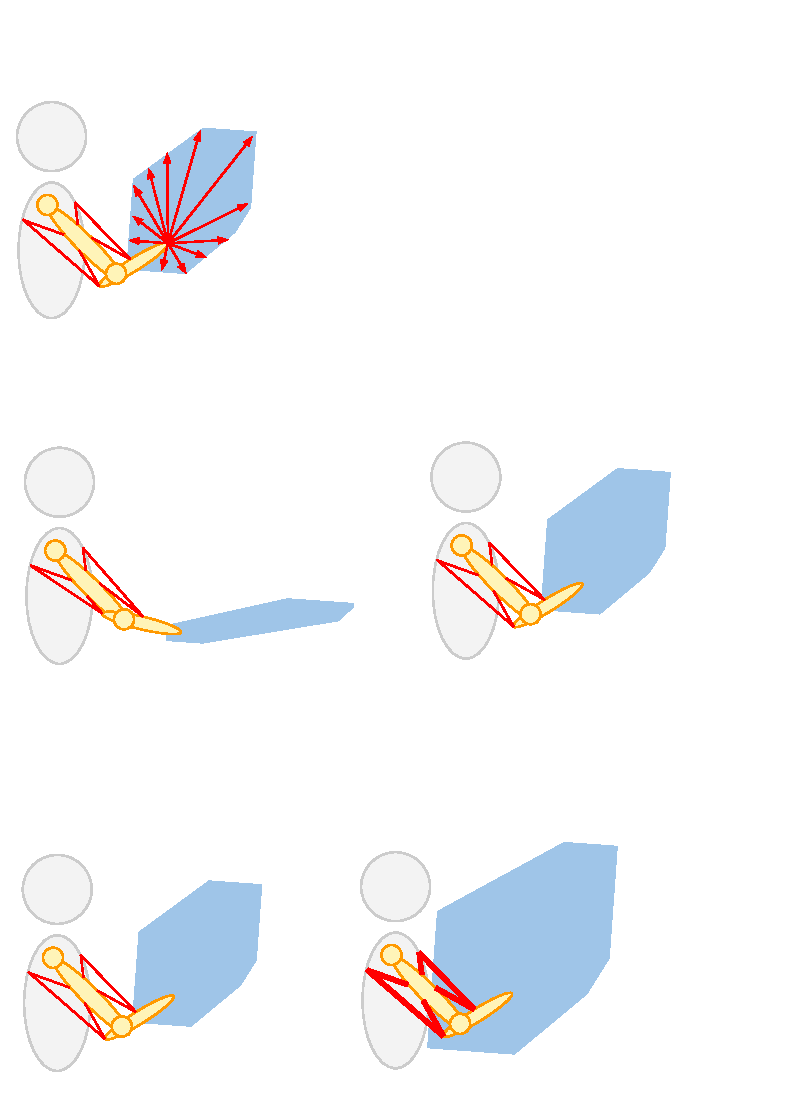
\includegraphics[trim={0 370 250 40},clip,width=0.3\linewidth]{img/chapter_1/ffs_characteristics.pdf}
    \caption{The \emph{force feasible set} of an individual in a specific posture denotes all maximally exertable forces in this upper-limb posture.}
    \label{fig:ffs_simple}
\end{figure}

Abstract mathematics emphasizes understanding how structures are preserved under transformations of their underlying elements. More interestingly, it also seeks to extract the original structure by analyzing the transformed elements. This approach is relevant for the study of maximal isometric forces. These forces, viewed as individual elements, are fundamentally derived from muscle activation patterns. A key goal of this thesis is to analyze the structure within these produced forces to gain insights into the collective behavior of muscle activations.

As such, the collection of all exertable maximal isometric forces at the hand constitutes the definition of a \emph{force feasible set} (Fig. \ref{fig:ffs_simple}). Since each element within this set depends on both upper-limb posture and individual physiology, this knowledge translates directly to its set-theoretic representation, as depicted in Figures \ref{fig:ffs_posture} and \ref{fig:ffs_individual}.
\begin{figure}[!htb]
    \captionsetup{justification=centering}
        \centering
        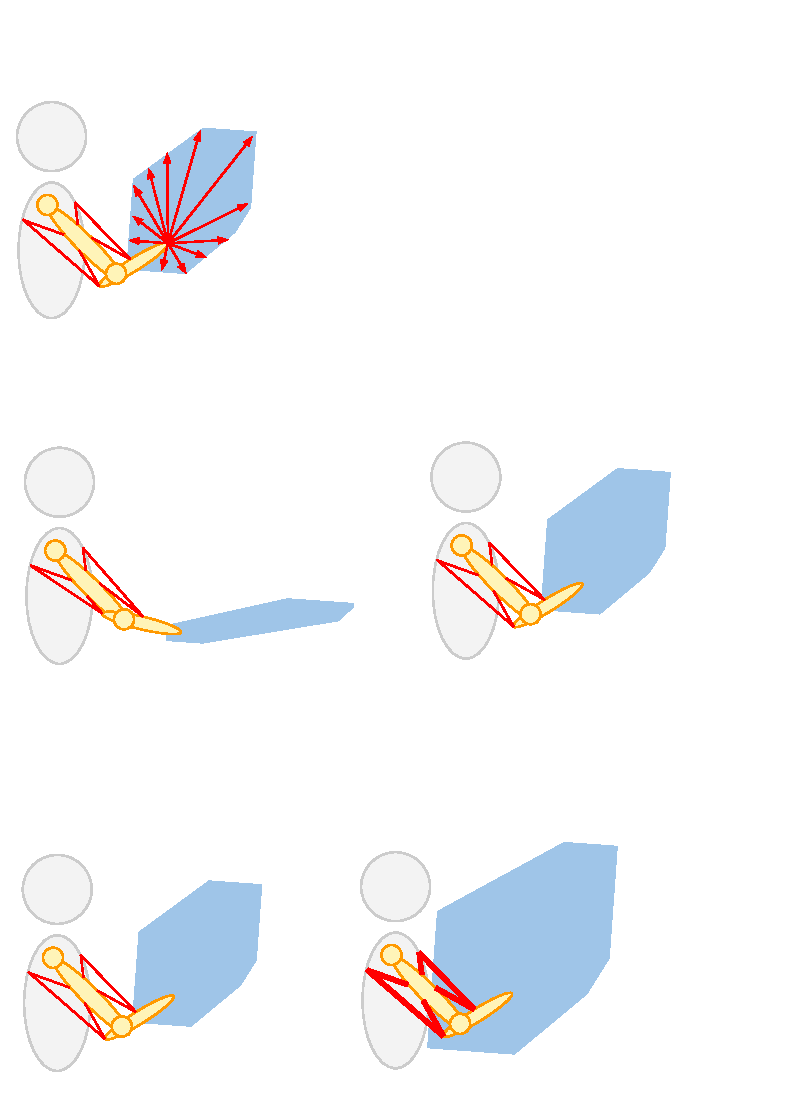
\includegraphics[trim={0 200 40 200},clip,width=0.7\linewidth]{img/chapter_1/ffs_characteristics.pdf}
    \caption{The force feasible sets of an individual vary according to a given posture.}
    \label{fig:ffs_posture}
\end{figure}


\begin{figure}[!htb]
    \captionsetup{justification=centering}
        \centering
        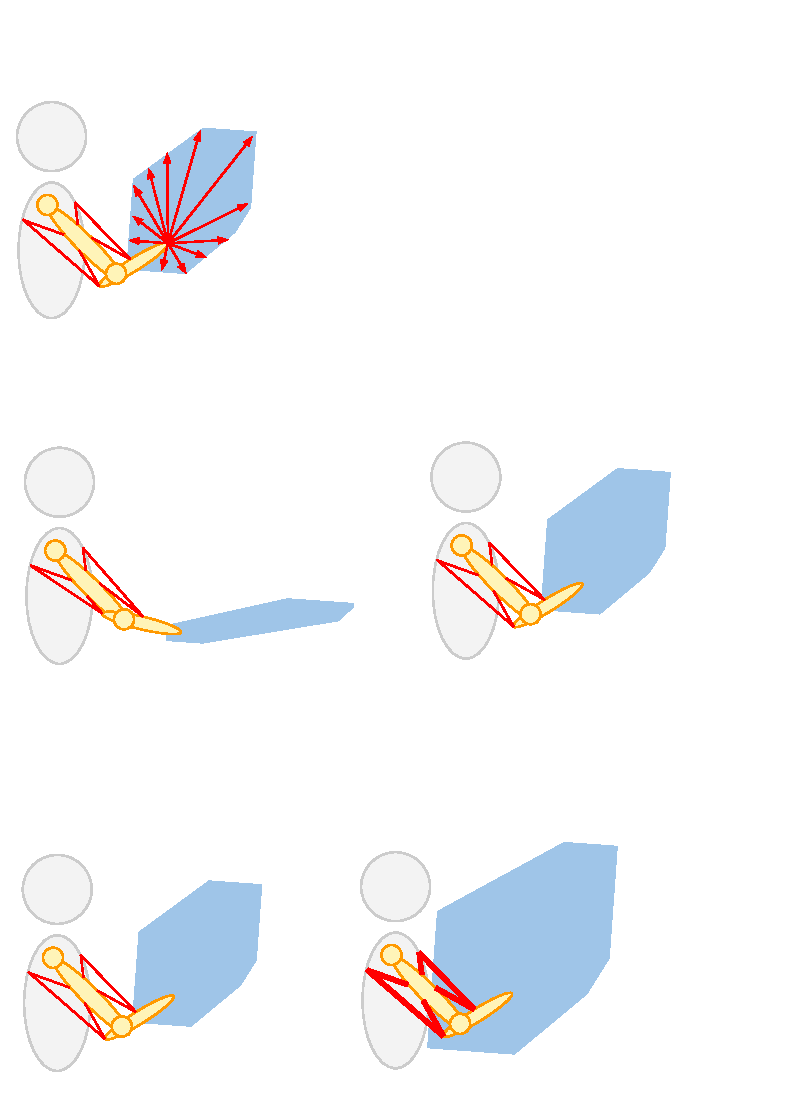
\includegraphics[trim={0 10 40 400},clip,width=0.7\linewidth]{img/chapter_1/ffs_characteristics.pdf}
    \caption{The force feasible sets of an individual vary depending on an individual's own physiology.}
    \label{fig:ffs_individual}
\end{figure}


Therefore, the set-theoretic perspective on force feasible sets offers significant potential, providing a concise way to convey to a robot biomechanical information about force boundaries producible in a human upper limb. Moreover, it allows leveraging the rich theoretical framework of modern mathematics to analyze and understand these sets, through various theoretical lenses (geometric, probabilistic, topological, etc.). Ultimately, a deeper understanding of force feasible sets can enhance the design and control of collaborative robots that interact effectively and safely with humans.

To explore this potential, this thesis will investigate the value of this set-theoretic approach in the context of personalizing musculoskeletal models in order to bring an answer to the following biomechanical challenge:

\begin{mdframed}
    \begin{center}
        \textbf{Challenge 3:} \\
        How can a set-theoretic approach to maximal isometric forces be used to quantitatively characterize muscle tension interactions
    \end{center}
\end{mdframed}

\section*{Thesis overview}
\addcontentsline{toc}{section}{Thesis overview}
This thesis involves the simulation of force feasible sets produced at the hand in a human upper-limb and their \emph{in vivo} counterparts. The different chapters contribute to a single objective: personalizing force feasible sets to an individual from maximal isometric force measurements in various postures. These chapters form a cohesive argument for this personalization process, creating a bridge between force feasible set modeling and biomechanical assumptions.

Chapter \ref{chapter:1} details how to derive force feasible sets, both \emph{in silico} and \emph{in vivo}, and examines the coherence between current modeling approaches and experimental measurements. Given the inherent set-theoretic nature of these representations, this chapter also explores current sensitivity analyses in biomechanics and considers more appropriate set-theoretic methods to assess how inter-individual muscle variability manifests in a set form.

Chapter \ref{chapter:2} delves into the computational challenges associated with the exact construction of a \emph{force polytope}, a force feasible set modeled under the assumption that muscle tensions are independent from each other. This construction necessitates computing either the vertices or the faces of a \emph{torque zonotope} representing all maximal joint torques generated by muscle tensions. The chapter introduces a novel vertex enumeration technique based on a specific selection of edges from a high-dimensional hypercube. This algorithm exhibits theoretical efficiency, with a time complexity comparable to the state-of-the-art. However, despite its efficiency, the inherent combinatorial complexity of vertex enumeration limits the applicability of this exact algorithm when the number of muscles exceeds a low amount ($>8$). Consequently, approximation alternatives are proposed for subsequent analyses in the thesis.

Chapter \ref{chapter:3} focuses on the theoretical implications of considering a high number of muscles in \emph{in silico} force feasible sets. This consideration is crucial because a force feasible set, by definition, reflects the combined action of all considered muscles, and its characteristics (volume, shape) are inherently dependent on the number of muscles included in the model. Simpler musculoskeletal models of the human upper limb may therefore fail to accurately capture experimentally observed force capacities. However, as demonstrated in the preceding chapter, increasing the complexity of the musculoskeletal model also increases the difficulty of modeling force feasible sets. To address this, the chapter draws upon established mathematical results from the \emph{Local Theory of Banach Spaces}, which investigates infinite-dimensional normed vector spaces through the lens of finite-dimensional ones, effectively bridging the gap between simplified models (seen as finite-dimensional spaces) and the complexities of real biological systems (represented as high-dimensional spaces). By applying these theoretical results to force feasible set modeling, the chapter argues that when a large number of muscles is considered, the \emph{size} (or \emph{scale}) of a force feasible set becomes the \emph{only} property influenced by muscle interactions. It demonstrates that any (convex) muscle interaction model induces force feasible sets which have the same ellipsoidal shape but with a size depending on the choice of the model. This scaling coefficient, termed the \emph{projection constant}, is explicitly computable for force polytopes and approximable for other tension models, enabling the construction of an ellipsoid approximation of a force polytope without resorting to computationally expensive combinatorial calculations. In other words, this chapter complexifies a musculoskeletal model in order to retrieve a simpler force feasible set representation as an ellipsoid.

Chapter \ref{chapter:4} focuses on quantifying the practical relevance of a set-theoretic approach to represent maximal isometric forces. We employ an optimization process to retrieve muscle parameterization in a 50-muscle musculoskeletal model (\cite{holzbaurModelUpperExtremity2005}), aiming to reproduce the default Holzbaur et al. force feasible sets in specific postures. Our methodology involves a careful analysis of the optimization results, considering factors such as different solving methods, posture sets, search-space sizes, parameters to be optimized, and force feasible set representations. Analyzing the solutions, the convergence of the algorithms, and their results for both polytopic and ellipsoidal force feasible set representations addresses the following questions:
\begin{enumerate}
    \item {\emph{Are 50 muscles sufficient to represent force feasible sets as ellipsoids?} The results suggest this is the case, as the generated force polytopes and their ellipsoid approximations yielded solutions with similar characteristics across almost all conditions in the optimization processes. This finding provides a practical lower bound on the number of muscles required for this approximation, supporting the theoretical results of the previous chapter, which indicated that the approximation holds in sufficiently \emph{high} dimensions;}
    \item {\emph{Is a set-theoretic approach relevant in musculoskeletal muscle personalization?} This analysis reveals that personalizing muscle parameters from force feasible sets in a real-world context is inherently challenging. While feasible in simpler cases with near-known solutions, the set-theoretic approach encounters significantly greater challenges in more complex scenarios. This difficulty is quantified through a novel index termed the \emph{enlargement ratio}, which relates the computational limitations of force polytope construction to the personalization process. By accounting for computational demands, we can assess the effectiveness of the personalization process and gain insights into the general difficulty of muscle personalization; }
    \item {\emph{Which muscle parameters most influence the force feasible set characteristics?} The results indicate a greater sensitivity to force-generating parameters compared to muscle geometry. Therefore, any such personalization process should prioritize the optimization of force-generating parameters.}
\end{enumerate}
These three findings directly inform the personalization process with \emph{in vivo} data in the next chapter.

Chapter \ref{chapter:5} integrates \emph{in silico} and \emph{in vivo} force feasible sets to generate personalized force capacities. An experimental protocol was conducted to collect maximal isometric force exertions at the hand in 26 directions and 4 postures from 10 participants. An upper-limb musculoskeletal model was then scaled to each participant. Building on Chapters \ref{chapter:3} and \ref{chapter:4}, which demonstrate the ellipsoidal nature of force polytopes, we utilize this approximation.  Furthermore, given the findings in Chapter \ref{chapter:4} regarding the limited influence of muscle geometry, we focus solely on adapting force-generating muscle properties. Also, Chapter \ref{chapter:2} highlighted that muscle tension interactions can be represented as a transformation of a sphere, providing a geometric interpretation for the ellipsoidal resemblance of force polytopes. This implies that individual muscle tension limits do not exert independent influence; rather, the average maximal tension across muscles primarily affects the scaling of a force feasible set. Consequently, only one parameter per posture require adjustment to align \emph{in silico} force feasible sets with \emph{in vivo} measurements. We apply this personalization process to the experimental data and evaluate the consistency of the theoretical results with empirical observations.

Finally, the Conclusion chapter will offer some closing remarks on this set-theoretic approach of maximal isometric forces, and draw the newest perspectives opened by the results found in this thesis. 

\section*{List of publications}
\addcontentsline{toc}{section}{List of publications}
During the thesis, two short publications were submitted and accepted. They are mentionned in Chapter \ref{chapter:4}, which focuses on muscle information extractable from force feasible sets. However, the work in these papers was preliminary to the work presented in Chapter \ref{chapter:4} and offered the first perspectives on the formulation of a muscle personalization process based on force feasible sets. The chapter serves as a more comprehensive exploration of these concepts, with a greater emphasis on the challenges of personalizing a musculoskeletal model, which neither paper addressed.

\begin{itemize}
    \item {G. Laisné, J-M. Salotti, and N. Rezzoug. ``Genetic Algorithms for Force Polytopes Prediction''. In: \emph{Computer Methods in Biomechanics and Biomedical Engineering} 26.sup1 (Oct. 2023), pp. 218-220.}
    \item {G. Laisné, J-M. Salotti, and N. Rezzoug. ``Derivative-Free Optimization Approaches for Force Polytopes Prediction''. In: \emph{ESANN 2023 - European Symposium on Artificial Neural Networks, Computational Intelligence and Machine Learning.} Bruges, Belgium, Oct. 2023, pp. 339-344.}
\end{itemize}

\section*{Notations}
\addcontentsline{toc}{section}{Notations}
This thesis employs a variety of mathematical objects, including vectors, matrices, lines, and sets, which are subject to manipulation and representation through diverse notational conventions. An example is the representation of a linear transformation between vector spaces by a matrix. While the notation may remain consistent, the context may necessitate an emphasis on either the matrix itself or the underlying linear transformation it encodes. This section serves to clarify the notational conventions for the objects employed in this thesis.

\begin{itemize}
    \item {\textbf{Common sets of numbers}: in uppercase and blackboard font. Examples: natural numbers $\mathbb{N}$, real numbers $\mathbb{R}$, strictly positive real number $\IR_{>0}$;}
    \item {\textbf{Bounded convex sets}: in uppercase, italic and caligraphic. Examples: cube $\mathcal{C}$, sphere $\mathcal{S}$, ellipsoid $\mathcal{E}$, polytope $\mathcal{P}$, zonotope $\mathcal{Z}$, orthotope $\mathcal{O}$;}
    \item{\textbf{Spaces}: in uppercase, italic letters. Examples: line $L$, plane $P$, hyperplane $H$, vector space $V$, Banach space $X$;}
    \item {\textbf{Coefficients}: in lowercase, italic and greek. Examples: $\lambda,\, \alpha,\, \mu \in\mathbb{R}$;}
    \item {\textbf{Points, integers and real numbers}: in lowercase, italic and latin. Examples: the points $p,\, q,\, r \in E$, the integers $n,\,m\in\mathbb{N}$ and the real $x\in \mathbb{R}$;}
    \item {\textbf{Vectors}: in lowercase, bold and latin. Vectors can be indexed by non-bold characters when needed. Examples: $\mathbf{x},\, \mathbf{y},\, \mathbf{q} \in \mathbb{R}^n$ and $\mathbf{x} = (x_1,\, \dots,\, x_n)$;}
    \item {\textbf{Matrices}: in uppercase, italic and block letters. Example: $M \in \mathbb{R}^{n\times m}$;}
    \item {\textbf{Functions}: in lowercase, italic and in latin or greek, with parentheses. Examples: the function $f\colon \mathbb{R}\rightarrow \mathbb{R}$ such that $f(x) = x^3$;}
    \item {\textbf{Affine maps}: An affine map denotes a linear mapping followed by a translation. The linear part can be represented by a matrix, and the translation by a vector. For instance, the linear transformation of a vector $\mathbf{x}\in\IR^3$ through $A \in \IR^{3\times 3}$, then translated by $\mathbf{t}\in\IR^3$, is noted $A\mathbf{x} + \mathbf{t}$. This notation is particularly useful for sets, where for instance the affine transformation of the 3D cube $\mathcal{C}=[0,1]^3$ under the same conditions is simply noted $A\mathcal{C} + \mathbf{t}$.}
\end{itemize}

\chapter{Force feasible set modeling}
\label{chapter:1}

\usection{Introduction}
For an individual, force exertion arises from complex interactions within the body, primarily involving the skeletal structure and musculature.  External factors, such as gravity, also influence force production. A \emph{force feasible set} of an individual is the representation of all his exertable forces at a specific point of application. This thesis focuses exclusively on linear forces, excluding the application of moments.

Due to their set-theoretic nature, force feasible sets provide a unique representation of the underlying biomechanical properties of the human body. They appear to encapsulate a greater amount of information compared to traditional biomechanical measures, as they encompass all possible force vectors. Since the exertion of force in a specific direction reflects the combined action of multiple muscles, analyzing the entire force feasible set allows for a comprehensive understanding of muscle coordination and force generation.

This set-theoretic framework, originating from robotics (\cite{yoshikawaManipulabilityRoboticMechanisms1985}; \cite{chiacchioForcePolytopeForce1997}), was initially used to characterize the force capabilities of robotic manipulators, specifically at the end-effector of a serial kinematic chain. The primary objective was to provide a compact representation of the limits of force exertion, enabling the determination, in silico, of whether a specific force magnitude and direction could be achieved. Drawing inspiration from robotics, this thesis adopts a serial kinematic chain model to represent certain human body segments, particularly the upper limb, with the end-effector corresponding to a point on the hand. This approach offers a significant advantage by enabling numerical simulation of force capabilities, circumventing the challenges associated with exhaustive experimental measurements of all exertable forces.

Section \ref{sec:muscu_model_in_silico_ffs} details the formalism required for this robotic-oriented approach to modeling the human upper limb, referred to as a musculoskeletal model. Various force feasible set representations are presented, along with their respective applications.  A major challenge in this set-theoretic approach lies in the computational complexity of set-based operations. These difficulties and current strategies for addressing them are discussed. In this regard, chapter \ref{chapter:2} introduces a novel algorithmic approach to mitigate these computational challenges in simulations.

Furthermore, the nature of the force feasible set inherently reflects how muscles combine to generate force at the end-effector. Different representations of force feasible sets employ specific assumptions regarding muscle coordination and tension combination. Section \ref{sec:modeling_muscle_tensions} will analyze these assumptions and their underlying biomechanical implications for several force feasible set representations found in the literature. As such, chapter \ref{chapter:3} will propose a more general framework for modeling muscle tension combinations. Chapters \ref{chapter:4} and \ref{chapter:5} will subsequently challenge the assumptions required to consider the validity of the presented framework, using \emph{in silico} and \emph{in vivo} maximal isometric forces. 

% Also, accurate numerical simulation necessitates an appropriate representation of the upper limb in silico.  Inter-individual variability in exertable forces arises from differences in anthropometry and muscle characteristics. To account for these individual-specific factors, personalization of musculoskeletal model parameters is essential, ensuring that simulated forces align with experimental data. A key objective of this thesis is to assess the efficacy of the force feasible set approach for this personalization process. Indeed, traditional personalization methods, relying on force measurements in specific directions, overlook the wealth of information embedded within force feasible sets. In this regard, while sensitivity analysis is commonly employed to evaluate the influence of biomechanical parameters on force exertion, the set-theoretic nature of force feasible sets presents challenges for traditional sensitivity analysis techniques. Section \ref{sec:feasibility_personalization} reviews existing methods for studying parameter influence and discusses the difficulties in adapting them to a set-theoretic framework. In response to this challenge, chapter \ref{chapter:4} presents a novel approach to sensitivity analysis that accommodates both set-based representations and muscle interactions.

\section{Musculoskeletal modeling and in silico force feasible sets}
\label{sec:muscu_model_in_silico_ffs}
This section focuses on modeling the human upper limb based on serial kinematic chains.

\subsection{Musculoskeletal models}
A musculoskeletal model is a biomechanical simulation tool that provides a quantitative representation of the human musculoskeletal system. It aims to replicate the anatomical structures as well as the biological and neuronal processes involved in human movement.
Applications of musculoskeletal models are observed in various fields. In biomechanics, they can be employed for estimating muscle forces and joint contact forces in order to understand injury mechanisms (\cite{renIdentificationKineticAbnormalities2022}), optimizing athletic performances (\cite{yeadonFiftyYearsPerformancerelated2023}), or designing rehabilitation strategies (\cite{weigelBiomechanicsRehabilitation2005}).
In ergonomics, these models aid in evaluating workplace design and identifying potential risk factors for musculoskeletal disorders (\cite{davidErgonomicMethodsAssessing2005}; \cite{granataLowBackBiomechanicsStatic2005}). Furthermore, they find applications in robotics, enabling the development of bio-inspired robots (\emph{anthropomorphic robots}) and their control strategies (\cite{aswiniBiomechanicsInspiredControlStrategies2023}).

By means of rigid body mechanics, muscle physiology, and joint kinematics, these models allow to investigate the internal dynamics of the musculoskeletal system.

A musculoskeletal model comprises a kinematic chain of rigid body segments, each representing a bone, interconnected by joints with defined \emph{degrees of freedom}. The degrees of freedom of a joint define its possible motions. Representing bones by rigid segments is a simplified skeletal representation, but its relevancy was proven through in various situations, such as accurately representing an individual bone to estimate articular mechanisms (\cite{suwargandaMinimalMedicalImaging2019}). These joints can be modeled as successive revolute joints (\emph{e.g.} the elbow flexion and forearm pronation-supination defined for the elbow, or the wrist flexion and deviation at the wrist), spherical joints or as more complex articulations with specific anatomical constraints. For example, De Groot and Brand modeled the shoulder joint motion (termed \emph{shoulder rhythm}) using linear regression equations to consider the interplay between motions of the clavicle, scapula, and humerus (\cite{degrootThreedimensionalRegressionModel2001}). Muscles are incorporated as force-generating elements that span between bone segments. They exert forces that induce joint moments, leading to a movement. As highlighted in (\cite{bassaniChapter15Musculoskeletal2018}), musculoskeletal modeling provides a powerful tool for non-invasive investigation, from healthy to pathological conditions, making its use highly relevant in various fields. The quality of these models can be enhanced by incorporating detailed muscle architecture and physiological properties. For instance, McNeill demonstrated the importance of tendon elasticity in jump analysis (\cite{mcneillalexanderTendonElasticityMuscle2002}). Furthermore, advanced models may include more specific muscle structures such as ligaments (\cite{shelburneMusculoskeletalModelKnee1997}).

Several softwares and libraries have been developped for simulations musculoskeletal model, including OpenSim (\cite{delpInteractiveGraphicsbasedModel1990a}), Biorbd (\cite{michaudBiorbdPythonMATLAB2021}), AnyBody (\cite{damsgaardAnalysisMusculoskeletalSystems2006}) and CusToM (\cite{mullerCusToMMatlabToolbox2019}).

\subsubsection*{Serial kinematic chains}
At the core of a musculoskeletal model is a kinematic chain: the representation of bones and how they are linked. For the upper limb, a serial kinematic chain can be considered. The following definition of such a chain is based on (\cite{lauGeneralizedModelingMultilink2013}).

A \emph{serial kinematic chain} consists of $k$ rigid bodies $B_1, \cdots, B_k$ linked successively via joints. For $i = 1, \cdots, k$, the joint between rigid bodies $B_{i-1}$ and $B_i$ describes the motion of body $B_i$ relative to $B_{i-1}$. We denote this joint $J_i$. In particular, if it is assumed that the joint has a fixed center of rotation, we denote the center of joint $J_i$ by $P_i$. Since joint $J_i$ can induce rotational as well as translational motions, body $B_i$ has a relative orientation and translation relative to $B_{i-1}$. To describe it, we define for each body $B_i$ a frame $\{F_i\}$ located at the body's center of mass $G_i$. When a joint configuration is fixed, it is thus possible to describe $B_i$'s frame and location according to the preceding $B_{i-1}$'s own frame and location through a rotation and translation mapping. For the first body $B_1$, its orientation and location are described according to the \emph{ground} notated $B_0$, which is assimilated to the origin of the space. The ground orientation and location are denoted $\{F_0\}$ and $O$ respectively. Figure \ref{fig:general_rigid_body_model} summarizes the serial kinematic chain formalism.
\begin{figure}[!htb]
    \captionsetup{justification=centering}
        \centering
        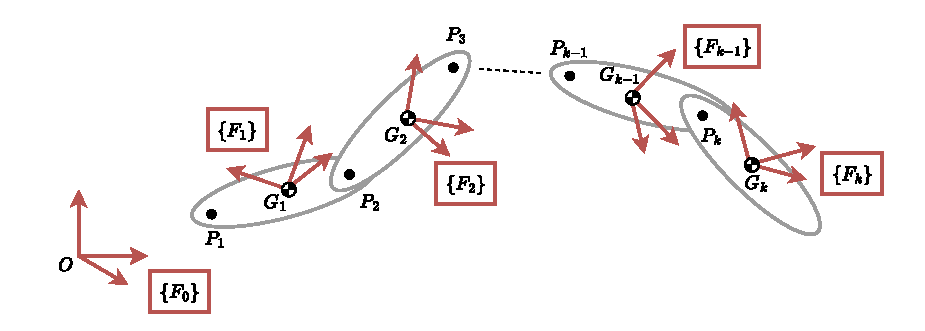
\includegraphics[trim={0 0 0 0},clip,width=1\linewidth]{img/chapter_4/general_rigid_body_model.pdf}
    \caption{Notations for a serial kinematic chain. The \emph{ground} $B_0$ is described via frame $\{F_0\}$ located at the origin $O$. A body $B_i$ is represented by a frame $\{F_i\}$ located at its center of mass $G_i$. Two bodies $B_{i-1}$ and $B_i$ are linked through a joint $J_i$ whose center is defined at point $P_i$. }
    \label{fig:general_rigid_body_model}
\end{figure}

A \emph{joint configuration} describes the specific positions of all the joints in a kinematic chain. It is defined by the values of the \emph{generalized coordinates}, which are parameters that quantify the different ways the joints can move.

Such serial kinematic chains assume that bodies are resistant to deformation, \emph{i.e.} they have infinite stiffness, and that joints' centers of rotation (points $P_1, \dots, P_k$) do not change their position for different joint configurations. However, this is not entirely sufficient for upper-limb modeling, as the scapulohumeral rythm affects internal forces, such as the glenohumeral joint force (\cite{flores-hernandezScapulothoracicRhythmAffects2019}). Since we focus on maximal forces produced at the hand of the upper limb, we need a more complex model to accurately capture essential biomechanical components required for further experimental validations. 

\subsubsection*{Actuators and muscle geometry}
While a serial kinematic chain can be actuated by controlling its joint torques or velocity, to better mimic human behavior, we should consider actuators. An actuator is a component that converts an energy source into motion. For instance, a cable-driven parallel robot could be powered by hydraulic cables. In the human body, muscles serve as actuators, converting chemical energy into mechanical force to produce movement.

The most commonly used muscle models are based on the Hill's model (\cite{hillHeatShorteningDynamic1938}). A Hill-type muscle model represents a musculotendon unit, comprising muscle fibers and a tendon, as a mechanical system with three interconnected elements. The contractile element simulates the active force generation of the muscle fibers.  A spring-like series elastic element, representing the tendon's elastic properties, is in series with the contractile element. Finally, a parallel elastic element accounts for the passive elasticity of the muscle tissue itself and acts in parallel with the other two elements. 

In order to study how a muscle acts on a joint to produce motion, muscle modeling requires consideration of two distinct aspects: the force amount and its line of action. These two facets are intrinsically linked through the force-length and force-velocity relationships, fundamental principles of biomechanics established in (\cite{hillHeatShorteningDynamic1938}). These relationships describe how muscle force varies depending on its length and velocity of contraction. Zajac summarizes these muscle properties in (\cite{zajacMuscleTendonProperties1989a}). However, while explicit computations can be formulated for the generated muscle force, determining the muscle line of action depends on factors such as muscle geometry, joint type, and surrounding anatomical structures. If the muscle geometry is determined to be similar to a single line segment (or straight cables), the action of the muscle onto a spherical joint of rotation center $P$ is quantifiable as a real vector $\tau\in \IR^3$ termed the \emph{muscle joint torque} and noted $\tau$. By considering $\mathbf{u}$ the normalized muscle line direction, $f$ the produced muscle force amount, and $A$ the orthogonal projection of $P$ onto the muscle line, then $\tau$ (in unit Newton-meter N$\cdot$m) is computed as 
\begin{align*}
    \tau = f\mathbf{u} \times (A - P)
\end{align*} 
where $\times$ is the cross product in $\IR^3$. To obtain the torque produced along a specific joint rotation axis $\omega\in \IR^3$, there suffices to compute $\omega \cdot \tau$, where $\cdot$ denotes the usual dot product. The distance $\| A - P \|$ is usually refered as the \emph{lever arm}, which represents the perpendicular distance from the joint center to the muscle's line of action.

While the line segment approximation for muscle geometry offers computational simplicity in calculating muscle joint torque, it fails to capture the complexities of more realistic muscle shapes.  To address this, a generalized coordinate approach can be employed. By defining the muscle length as a function of generalized coordinates, $l(\mathbf{q})$, the muscle joint torque, $\tau$, about a joint axis $\omega$ can be determined through the partial derivative of the length function with respect to the generalized coordinates:
\begin{align*}
    \tau = \frac{\partial l(\mathbf{q})}{\partial \mathbf{q}}
\end{align*}

This formulation accommodates any continuous muscle path, provided the length function is differentiable. However, differentiating this function can be challenging, often necessitating numerical differentiation techniques or optimization algorithms, as employed in OpenSim musculoskeletal modeling software (\cite{delpOpenSimOpenSourceSoftware2007}).

The choice between simplified and complex muscle geometries depends on the specific application and desired level of accuracy. For instance, (\cite{livetAutomaticSimplifiedApproach2022}) consider that muscles are described as successive rigid segments connected by \emph{via points}. In (\cite{kedadriaShoulderMusculoskeletalModel2023}), the authors highlights the benefits of refined muscle geometry modeling. Their study demonstrated that detailed representations of muscle fiber paths, particularly in the shoulder, yield muscle moment arms that more closely align with experimental cadaveric data from (\cite{acklandMomentArmsMuscles2008}) than those obtained through simplified segment approximations. This suggests that incorporating more realistic muscle geometries can enhance the accuracy and fidelity of musculoskeletal models. In this regard, we will therefore consider the general case of complex muscle geometry models.

Enhancing the efficiency of complex musculoskeletal computations, particularly those involving moment arm calculations, has driven the exploration of alternative approaches to muscle geometry modeling. However, recent research has investigated the use of polynomial functions to represent muscle length and moment arms.

For instance in (\cite{menegaldoMomentArmsMusculotendon2004}), the authors employed polynomials to model 43 lower limb muscles in the lower extremity musculoskeletal model developed in (\cite{delpInteractiveGraphicsbasedModel1990a}). Their analysis of the tibialis anterior muscle revealed a maximum error of 0.15 cm in the computed moment arm surface across a wide range of ankle and subtalar joint angles, with the largest errors occurring near the joint limits.  While this study focused on predicting muscle moments, it did not explicitly evaluated the accuracy of muscle length estimations.
In (\cite{sobinovApproximatingComplexMusculoskeletal2020}), the authors utilized higher-order polynomials (order 6) to represent upper limb muscles. Their findings indicated promising accuracy for both muscle length and moment arms across various joint configurations, with errors below 5$\%$ compared to geometric computations for both measures. However, despite their computational advantages, the authors noted that the accuracy of these polynomial models depended on the quality of the data used to generate them. Specifically, they observed increased force and torque errors with increasing noise levels in the input muscle length and moment arm data. For example, 10$\%$ noise in the input data resulted in a 7.36$\%$ error in produced force and a 61.2$\%$ error in torque compared to expected values.

To ensure the accurate representation of muscle action and align with experimental findings reported in the literature, this thesis will employ complex muscle geometries that reflect experimentally measured moment arm data. Furthermore, muscle force production will be modeled using the Hill-type model, a widely adopted and experimentally validated approach in the field of biomechanics.

\subsection{Force feasible sets formalism}
We now examine how muscles generate forces across joints to produce forces at the hand. This will lead to the characterization of the feasible force sets, which represent the range of forces that can be generated by the combined action of the upper limb muscles.

\subsubsection*{Tension feasible set}
In (\cite{hillHeatShorteningDynamic1938}), the author described initially a mechanical model of two components, one representing a muscle and the other a tendon. Combined into one system, these composants form the \emph{musculotendon unit}. Current Hill-based models comprise three components: 1) the \emph{contractile element} (CE), which corresponds to the contractile properties of fibers inside the muscle part; 2) the \emph{passive elastice element} (PEE), which encompasses the elastic properties of these fibers and is in parallel with the contractile element; and 3) the \emph{serial elastic element} (SEE), which reflects the elastic properties
of the tendon in the musculotendon unit and is series with the first two components. Figure \ref{fig:hill_mech_model} summarizes this model.
\begin{figure}[!htb]
    \captionsetup{justification=centering}
    \centering
    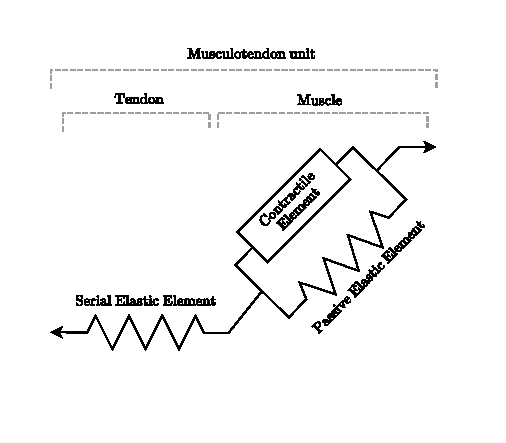
\includegraphics[trim={20 30 30 15}, clip, width=0.5\linewidth]{img/chapter_1/hill_mechanical_model.pdf}
    \caption{Hill's muscle model (\cite{hillHeatShorteningDynamic1938}). Forces exerted by a tendon are modeled via a spring is series with the muscle forces modeled in two parts: a contractile element in parallel with a spring.}
    \label{fig:hill_mech_model}
\end{figure}

Hill discovered a relationship between forces $f^M$ (in Newton) produced by a muscle and its length $l^M$ (also termed \emph{fiber} length) as well as its velocity $\dot(l^M)$. Since this thesis focuses on isometric condition, \emph{i.e.} $\dot{l^M} = 0$, we will describe the muscle force-length relationship only. For this, we consider the \emph{activation} of a muscle, \emph{i.e.} how much it should contract. The activation is controlled by a neural command, and is represented as a positive real value $a\in [0,1]$. In isometric condition, where activation is at $1$, the contractile element of a muscle produces its peak force $f_{iso}$, termed the \emph{maximal isometric force}, at a specific length $l_o$, the \emph{optimal fibel length}. When the contractile part has a smaller or larger length than $l_o$, the produced force decreases. For other activation states, this force is proportional to the activation. These relationships specifically describe the force produced by the contractile component of Hill's muscle model, which is termed the \emph{active force} $f_A$. The passive muscle element also exerts forces $f_P$, as it is modeled as a non-linear spring: these depends on the muscle length and are termed \emph{passive forces}. Since both active and passive forces are modeled in parallel, the total muscle force is the sum of their respective produced forces.
Figure \ref{fig:force_length_activation} describes these relations as curves.
\begin{figure}[!htb]
    \captionsetup{justification=centering}
    \begin{minipage}{0.49\linewidth}
        \centering
        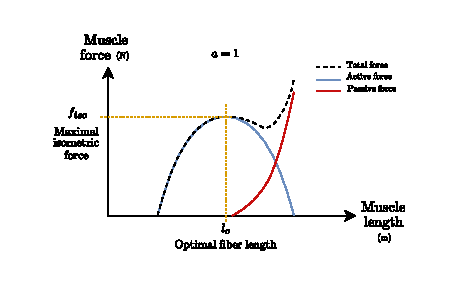
\includegraphics[trim={20 10 25 10}, clip, width=1\linewidth]{img/chapter_1/hill_force_length_relationship_fully_act.pdf}
    \end{minipage}
    \hfill
    \begin{minipage}{0.49\linewidth}
        \centering
        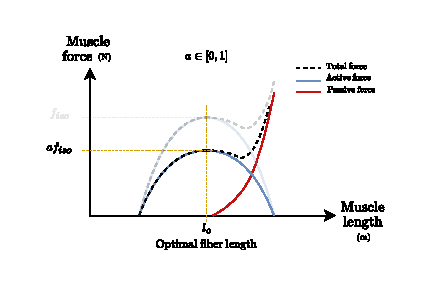
\includegraphics[trim={20 10 20 10}, clip, width=1\linewidth]{img/chapter_1/hill_force_length_relationship_all_act.pdf}
    \end{minipage}
    \caption{Simplification of Hill's force-length relationship in a muscle. When a muscle is fully activated ($a=1$, left figure), the muscle \emph{maximal isometric force} $f_{iso}$ is produced when the muscle length is at its \emph{optimal fiber length} $l_o$. In general (right figure), when the muscle activation varies, the active force-length curve is proportional to the activation, and so is the maximal force.}
    \label{fig:force_length_activation}
\end{figure}

However, the musculotendon unit is not a straight line, so to account for the non-linear shape of the musculotendon unit, both tendon and muscle are assumed to be separate segments with different lengths. The tendon is assumed to be bonded to the attaching bone, so that its produced force $f^T$ is along the bone's direction. In contrast, muscle fibers are \emph{pennated}, \emph{i.e.} there is a non-negligible angle $\alpha \in [0, \pi]$ between the tendon and the muscle segments. To account for this pennation angle, the produced muscle force $f^M$ is orthogonally projected onto the tendon's direction. 
\begin{figure}[!htb]
    \captionsetup{justification=centering}
    \centering
    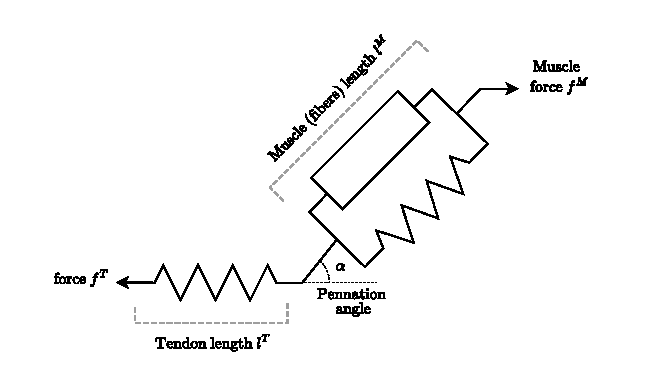
\includegraphics[trim={20 15 30 15}, clip, width=0.6\linewidth]{img/chapter_1/hill_mechanical_force_model.drawio.pdf}
    \caption{Forces in Hill's muscle model.}
    \label{fig:hill_mech_model_forces}
\end{figure}

When isometric conditions are assumed, the tendon force $f^T$ and muscle force $f^M$ are identical, and the muscle force-length relationship can be described as follows:
\begin{align*}
    f^M = f_{iso}(af_A(l^M) + f_P(l^M))\cos (\alpha)
\end{align*}
where $a\in [0,1]$ is the muscle activation, $\alpha\in [0, \pi]$ the pennation angle, $f_A$ is the normalized active force curve and $f_P$ is the normalized passive force curve, in which the given muscle lengths $l^M$ are normalized by the optimal fiber length $l_o$.

Another important muscle parameter is the tendon slack length $l_s$.
Tendons stretch and recoil during movement, and and because its force behavior is modeled as a spring, the tendon produces its own force $f^T$ depending on its own length $l^T$. Similarly to the passive elastic element of the muscle part, the tendon produces force when it is stretched beyond a certain length, termed the \emph{tendon slack length} and noted $l_s$.

However, in isometric conditions the forces occurring within the musculotendon unit balance each other, so that the muscle force equals the tendon force. Hill's model also incorporates muscle velocity and a force-velocity relationship, which describes how the force a muscle can generate depends on its speed of contraction. Elastic elements could also be considered to have visco-elastic properties, so that their velocities also influence their forces. However, this thesis focuses only on isometric conditions, so we do not need to consider any velocity-related properties for force-generation within the musculotendon unit.

It is to be noted that the forces generated within the musculotendon unit are considered positive when acting in their direction of application. The term \emph{tension} is therefore used to emphasize that these forces are always considered positive, acting in the direction that pulls on the tendon. 
% The biomechanical model of a muscle being defined in isometric conditions, we shall concentrate on explicitely descrbe the active and passive force-length curves.

% \paragraph*{The Hill-Thelen muscle model.}

The \emph{feasible tensions of a muscle} refer to the set of all tensions exertable by a muscle for a specific length. Since its tension depends on its length, the feasible tensions of a muscle reflect the possible tensions achievable solely through varying the activation level. When considering a musculoskeletal model and one of its muscle $M$, its feasible tension set is noted $\mathcal{T}^M$ and is defined as follows:
\begin{align*}
    \mathcal{T}^M &= \left\{ t\in \IR_{\geq 0} \mid t = f_{iso}(af_A(l^M) + f_P(l^M))\cos (\alpha),\quad a\in [0,1]\right\} \\
    &= [\underline{t^M}, \, \overline{t^M}]
\end{align*}
where $\underline{t}^M = \min \mathcal{T}^M$ and $\overline{t}^M = \max \mathcal{T}^M$. 

Since a musculoskeletal model may consist of multiple muscles, the \emph{tension feasible set} (of the musculoskeletal model) denotes all muscle tension combinations producible by all muscles. It is noted as $\mathcal{T}$ and is a subset of a $m$-dimensional real space, where $m$ is the number of considered muscles. This set depends on the specific posture of the musculoskeletal system, as muscle lengths change with joint angles.

Different combinations of muscle tensions reflect different biomechanical assumptions. For instance, if we define for a posture $\mathcal{T}$ as:
\begin{align*}
    \mathcal{T} = \left\{ \mathbf{t}=(t_1,\dots,t_m)\in\IR^m \mid t_i \in [\underline{t_i}, \, \overline{t_i}],\, \forall i=1,\dots, m \right\}
\end{align*} 
then $\mathcal{T}$ is a $m$-dimensional hyperrectangle, also termed $m$-\emph{orthotope} (\emph{c.f.} Figure \ref{fig:tension_set_orthotope_example}). This implies that all muscles can be fully activated at the same time.
\begin{figure}[!htb]
    \captionsetup{justification=centering}
    \centering
    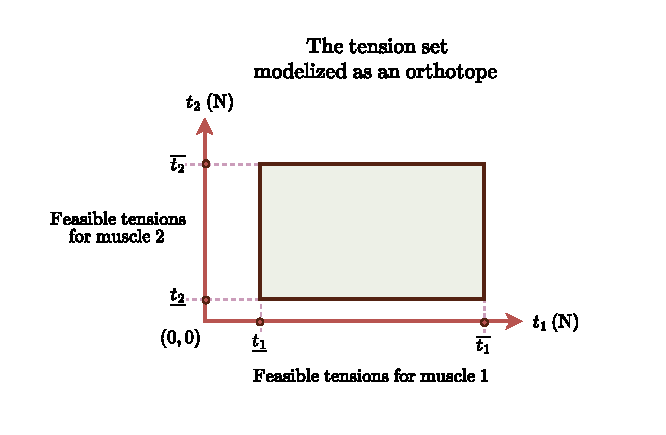
\includegraphics[trim={25 20 40 16}, clip, width=0.6\linewidth]{img/chapter_2/tension_set_orthotope.pdf}
    \caption{A muscle exerts a tension in a feasible range of values. The set of all tension combinations $\mathcal{T}$ is shaped as an \emph{orthotope} (or \emph{hyperrectangle}): it assumes muscles act independently from each other.}
    \label{fig:tension_set_orthotope_example}
\end{figure}

Having defined the tension feasible set, we will now formulate the force feasible set formulation by showing how the equation of motion relates muscle tensions to the forces produced at the hand.

\subsubsection*{The equation of motion}
In a dynamical context, the serial kinematic chain of a considered musculoskeletal model is described by $n$ generalized coordinates associated to $n$ degrees of freedom. We shall consider the parametrization of the degrees of freedom as a vector of \emph{generalized coordinates} $\mathbf{q} = (q_1, \dots, q_n)\in \IR^n$, and also consider the generalized velocities $\dot{\mathbf{q}} = (\dot{q}_1, \dots, \dot{q}_n)\in \IR^n$ and the generalized accelerations $\ddot{\mathbf{q}} = (\ddot{q}_1, \dots, \ddot{q}_n)\in \IR^n$. These vectors describe the kinematic chain's configuration and how it is changing over time. Each rigid body $B_i$, for $i = 1,\dots, k$ has a positive mass $m_i$ (in kg). To describe how this mass is distributed throughout the kinematic chain and how it affects the system's resistance to acceleration, we define the inertia matrix of the musculoskeletal model. Importantly, this matrix depends on the joint configuration $\mathbf{q}$. We denote by $C(\mathbf{q}, \dot{\mathbf{q}})$ the Coriolis and centrifugal torques. These are velocity-dependent forces that arise due to motions in the kinematic chain and the joints between its links. $\mathbf{G}(\mathbf{q}) \in \IR^n$ denotes the vector of gravitational torques.
Finally, $\tau\in \IR^n$ denotes the vector of \emph{joint torques} and describes the forces applied by the actuators at each joint to drive the motion.

The \emph{equation of motion} (\cite{lauGeneralizedModelingMultilink2013}; \cite{skuricCoupledViewPhysical}) is thus described as a differential equation of the generalized coordinates:
\begin{align*}
    M(\mathbf{q})\ddot{\mathbf{q}} + C(\dot{\mathbf{q}}, \mathbf{q})\dot{\mathbf{q}} + \mathbf{G}(\mathbf{q}) = \tau
\end{align*}

The surrounding space for $\tau$ vectors is termed the \emph{torque space}, and is of dimension the number of generalized coordinates, which we will assume is equal to the number of degrees of freedom.
Joint torque vectors $\tau$ are produced by actuators and other forces in the musculoskeletal model. 

On one hand, a force $\mathbf{f}$ applied at an end-effector point $X = (x_1, x_2, x_3)\in \IR^3$ is projected linearly onto the torque space. Indeed, the Jacobian matrix at point $X$ for joint configuration $\mathbf{q}$, $J_X(\mathbf{q})\in \IR^{3\times n}$, which relates the velocities of the generalized coordinates $\dot{\mathbf{q}}$ to the Cartesian velocities of the end-effector $\dot{X}$, describes how a change in the generalized coordinates results in a change of a Cartesian position:
\begin{align*}
    \dot{X} = J_X(\mathbf{q})\dot{\mathbf{q}}
\end{align*}
where $J_X(\mathbf{q}) = \left(\frac{\partial x_i}{\partial q_j}\right)_{i,j}$ for $i=1,2,3$ and $j=1,\dots, n$. Due to kineto-static duality, which relates forces and velocities in a mechanical system, the transpose of $J_X(\mathbf{q})$, noted $J_X^T(\mathbf{q})$ relates a linear force $\mathbf{f}\in\IR^3$ at $X$ to the joint torques as follows:
\begin{align*}
    \tau = J_X^T(\mathbf{q})\mathbf{f}
\end{align*}

On the other hand, the length $l_i$ of muscle $i$, for $i=1,\dots, m$, depends on the joint configuration $\mathbf{q}$. The muscle velocities $\dot{\mathbf{l}} = (\dot{l}_1, \dots, \dot{l}_m)\in \IR^m$ are described through the linear mapping $L\in\IR^{m\times n}$, which relates the rates of change of muscle lengths to the velocities of the generalized coordinates: 
\begin{align*}
    \dot{\mathbf{l}} = L(\mathbf{q})\dot{\mathbf{q}}
\end{align*}
where $L(\mathbf{q}) = \left(\frac{\partial l_i}{\partial q_j}\right)_{i,j}$ for $i=1,\dots, m$ and $j=1,\dots, n$. $L$ is termed the \emph{lever arm} matrix. Similarly to the Jacobian matrix, the transpose of $L$ relates the muscle tensions $\mathbf{t}\in\IR^m$ to the joint torques via:
\begin{align*}
    \tau = -L^T(\mathbf{q})\mathbf{t}
\end{align*}
The negative sign in this equation reflects the sign convention used for muscle forces and joint torques. For instance, when the biceps muscle contracts (positive tension), it creates a flexion torque at the elbow, which is represented as a negative torque in the equation since the positive direction for the elbow angle is extension

When no other actuators or forces are considered, the equation of motion is written as:
\begin{align*}
% \label{eq:equa_motions_muscle}
    M(\mathbf{q})\ddot{\mathbf{q}} + C(\dot{\mathbf{q}}, \mathbf{q})\dot{\mathbf{q}} + \mathbf{G}(\mathbf{q}) + J_X^T(\mathbf{q})\mathbf{f} = -L^T(\mathbf{q})\mathbf{t}
\end{align*}

We will now formulate the force feasible set, for both dynamic and static cases.

\subsubsection*{General formulation of force feasible sets}
As described in (\cite{skuricCoupledViewPhysical}), the \emph{force feasible set} $\mathcal{F}_X^{\mathcal{T}}(\mathbf{q}, \dot{\mathbf{q}}, \ddot{\mathbf{q}})$ at joint configuration $(\mathbf{q}, \dot{\mathbf{q}}, \ddot{\mathbf{q}})$ is defined to be the set of all forces $\mathbf{f}(\mathbf{q}, \dot{\mathbf{q}}, \ddot{\mathbf{q}})$ such that there exist muscle tensions satisfying the equation of motion:
\begin{align*}
% \label{eq:ffs_general}
    \mathcal{F}_X^{\mathcal{T}}(\mathbf{q}, \dot{\mathbf{q}}, \ddot{\mathbf{q}}) = \left\{\mathbf{f}\in\IR^3 \mid \exists \mathbf{t}\in \mathcal{T}(\mathbf{q}, \dot{\mathbf{q}}),\, M(\mathbf{q})\ddot{\mathbf{q}} + C(\dot{\mathbf{q}}, \mathbf{q})\dot{\mathbf{q}} + \mathbf{G}(\mathbf{q}) + J_X^T(\mathbf{q})\mathbf{f} = -L^T(\mathbf{q})\mathbf{t}\right\}
\end{align*}

\subsubsection*{Force feasible sets in isometric conditions}
In \emph{isometric conditions}, muscles are contracting but are not shortening or lengthening, meaning the musculotendon forces are in a static equilibrium state where the generalized velocities and accelerations of the kinematic chain are $\dot{\mathbf{q}}=0$ and $\ddot{\mathbf{q}} = 0$. We use the term \emph{posture} to refer to a joint configuration $\mathbf{q}$ where the velocities and accelerations are null.

Force feasible sets in isometric conditions are described for a given posture $\mathbf{q}$ as follows:
\begin{align*}
% \label{eq:ffs_description_static}
    \mathcal{F}_X^{\mathcal{T}}(\mathbf{q}) = \left\{\mathbf{f}\in\IR^3 \mid \exists \mathbf{t}\in \mathcal{T}(\mathbf{q}), \quad \mathbf{G}(\mathbf{q}) + J_X^T(\mathbf{q})\mathbf{f} = -L^T(\mathbf{q})\mathbf{t} \right\}
\end{align*}

It corresponds to the set of forces applied at the end effector such that the gravity and a combination of muscle forces can compensate for the applied force. Throughout this thesis, the term \emph{force feasible set} will be used exclusively to refer to the \emph{force feasible set in isometric conditions}. 

Before delving into force feasible set computations, we introduce more compact notations to improve readability. When possible, we will denote a force feasible set $\mathcal{F}_X^{\mathcal{T}}(\mathbf{q})$ as $\mathcal{F}(\mathbf{q})$, and simply as $\mathcal{F}$ when the posture is clear from the context or not relevant. Since the relevant tension feasible set will always be defined beforehand, the subscript $\mathcal{T}$ can be omitted. Furthermore, forces will generally be applied at the right hand of an upper-limb musculoskeletal model, since this thesis focuses exclusively on forces applied at the right hand. The coordinates of $X$ will be specified when relevant, such as during \emph{in silico} or \emph{in vivo} experiments. However, even when the coordinates of $X$ are specified, the $X$ subscript will be omitted from the force feasible set notation. Thereforce, $\mathcal{F}(\mathbf{q})$ will always denote a force feasible set with an underlying tension feasible set (defined beforehand) and a point of application $X$. Consequently, it is also common to denote the Jacobian transpose computed at point $X$ as $J^T(\mathbf{q})$, omitting the $X$ subscript.

Since the force feasible set depends on the posture $\mathbf{q}$, it is often expressed as a function of $\mathbf{q}$. This highlights the fact that the set of feasible forces changes as the posture changes. For brevity, we will often omit the explicit dependence on $\mathbf{q}$ in the notation for force feasible sets, where it is understood that all elements in the set's definition implicitly depend on $\mathbf{q}$:
\begin{align*}
    \mathcal{F} = \left\{\mathbf{f}\in\IR^3 \mid \exists \mathbf{t}\in \mathcal{T}, \quad J^T\mathbf{f} = -L^T\mathbf{t} - \mathbf{G}\right\}
\end{align*}

The force feasible set formulation is a geometric transformation of the tension feasible set $\mathcal{T}$. To highlight the underlying geometry, we can express this relationship in an alternative form. Let $\mathcal{F}$ be the force feasible set at end-effector $X$ for a given posture and a tension feasible set $\mathcal{T}$. Then, $\mathcal{F}$ can be expressed, up to linear transformation, as:
\begin{align*}
    \im{J^T} \cap \left(-L^T\mathcal{T}-\mathbf{G}\right)
\end{align*}
where $-L^T\mathcal{T}-\mathbf{G} = \left\{\tau\in \IR^n\mid \exists \mathbf{t}\in\mathcal{T},\quad \tau = -L^T\mathbf{t} - \mathbf{G} \right\}$ is the \emph{torque feasible set} and representing all torques achievable through muscle tensions and gravity. Also, $\im{J^T}$ denotes the \emph{image} of the matrix $J^T$, which is the vector space spanned by its columns. We will assume that $\dim \im{J^T}$ is $3$, or more generally, $p$, where $p$ is the rank of $J^T$. Therefore, $\im{J^T}$ is a subspace of the $n$-dimensional torque space. If $J^T$ is invertible, then $\im{J^T}$ spans the entire torque space. This implies that every exertable force at the end-effector corresponds to a unique combination of joint torques, indicating no redundancy in the system.

The sets $\mathcal{F}$ and $\im{J^T} \cap \left(-L^T\mathcal{T}-\mathbf{G}\right)$ are considered \emph{equivalent up to linear transformation}. This means that they are not \emph{strictly} identical, but they represent the same underlying set viewed from two different perspectives: the Cartesian force space, where forces are expressed in Cartesian coordinates ($\mathbf{f}\in \IR^3$), and the torque space, where they are expressed as joint torques ($J^T\mathbf{f}\in \IR^n$). When expressed in the torque space, the force feasible set $\mathcal{F}$ becomes $J^T\mathcal{F} := \left\{\tau\in \IR^n \mid \exists \mathbf{f}\in \mathcal{F}, \quad \tau = J^T\mathbf{f}\right\}$. 
To map forces from the torque space back to the Cartesian force space, we can use the \emph{Moore-Penrose pseudo-inverse of $J^T$}, denoted $(J^T)^+$, and we have $\mathcal{F} = (J^T)^+(J^T\mathcal{F})$, which recovers the original force feasible set in Cartesian coordinates. The (left) Moore-Penrose pseudo-inverse $(J^T)^+$ is defined as:
\begin{align*}
    (J^T)^+ = (JJ^T)^{-1}J
\end{align*}
which satisfies the property $(J^T)^+J^T = I_3$, where $I_3$ is the $3\times 3$ identity matrix.

For conciseness, we can consider the force feasible set $\mathcal{F}$ in either the Cartesian force space or the torque space. This is justified by the fact that an invertible linear transformation, which can be computed for any given posture, allows us to seamlessly switch between these two representations.

\subsection{Force feasible sets computation}
Given a tension feasible set $\mathcal{T}$, the force feasible set $\mathcal{F}$ can be described as two successive geometric operations: a \emph{projection} of $\mathcal{T}$ onto the torque space, creating the \emph{torque feasible set}, which is then \emph{intersected} by $\im{J^T}$, yielding the force feasible set $\mathcal{F}$ expressed in the torque space (\cite{skuricCoupledViewPhysical}). This modeling of forces is based on a rigid-body framework, which may not fully capture the complexities of deformable systems. Nevertheless, we assume throughout this thesis that bones are non-deformable. The force feasible set geometric construction can be summarized as follows:
\begin{figure}[!ht]
    \centering
    \captionsetup{justification=centering}
    \begin{tikzcd}
        \mathcal{T} \arrow[rr, "\text{projection}"'] &  & -L^T\mathcal{T}-\mathbf{G} \arrow[rr, "\text{intersection}"'] &  & J^T\mathcal{F} \arrow[r, "(J^T)^+"', bend right] & \mathcal{F} \arrow[l, "J^T"', bend right]
    \end{tikzcd}
    % \caption{Description of the geometric operations to derive the force feasible set in isometric conditions. The set of muscle tensions $\mathcal{T}$ is projected and translated onto the torque space to create the torque feasible set $\mathcal{T}_o$. It is then intersected with a vector space ($\im J^T$) to produce the force feasible set $\mathcal{F}$ described in the torque space, or conveniently in the Cartesian force space using $(J^T)^+$. In practice, we prefer to express $\mathcal{F}$ in the torque space since $(J^T)^+$ is a bijection between $\mathcal{F}$ and $\mathcal{F}'$.}
    % \label{fig:segsd}
\end{figure}

Throughout this thesis, we use the term \emph{projection} in a generalized sense to highlight that the muscle tension space is related to the torque space through a surjective affine mapping, which consists of a surjective linear mapping ($-L^T$) followed by a translation ($-\mathbf{G}$). 
Since this mapping is surjective, the dimension of the torque space is less than that of the muscle tension space, implying that there are more muscles than degrees of freedom. The use of the term \emph{projection} here emphasizes the surjective nature of this mapping and should not be confused with the typical notion of an orthogonal projection.

The \emph{projection-intersection} process described above involves two main computations: projecting the tension feasible set onto the torque space and intersecting the resulting set with the image of the Jacobian transpose. Each of these computations requires distinct techniques, largely determined by the geometry of the tension feasible set $\mathcal{T}$.

If we assume that $\mathcal{T}$ is a cube or an orthotope, then $\mathcal{F}$ is a \emph{bounded convex polytope} (or simply \emph{polytope}), which is a generalization of a 2D convex polygon to $n$ dimensions (\cite{grunbaumConvexPolytopes2013}). A set is \emph{convex} if the line segment connecting any two points in the set is also contained within the set. A set is \emph{bounded} if it can be contained in a ball of finite radius. A polytope, by definition, includes all of its interior points as well as the points on its surface. 

Alternatively, the tension feasible set $\mathcal{T}$ could be a ball or an ellipsoid, which includes all of its interior points. In this case, the boundary of the force feasible set is an ellipsoid. Figure \ref{fig:tension_models_on_ffs} summarizes these different constructions.

\begin{minipage}{0.4\linewidth}
    \centering
    $\mathcal{T}$ is a cube, so $\mathcal{F}$ is a polytope.
\end{minipage}
\hfill
\begin{minipage}{0.4\linewidth}
    \centering
    $\mathcal{T}$ is a ball, so $\mathcal{F}$ is an ellipsoid.
\end{minipage}
\begin{figure}[!htb]
    \centering
    \captionsetup{justification=centering}
    \begin{minipage}{0.48\linewidth}
        \centering
        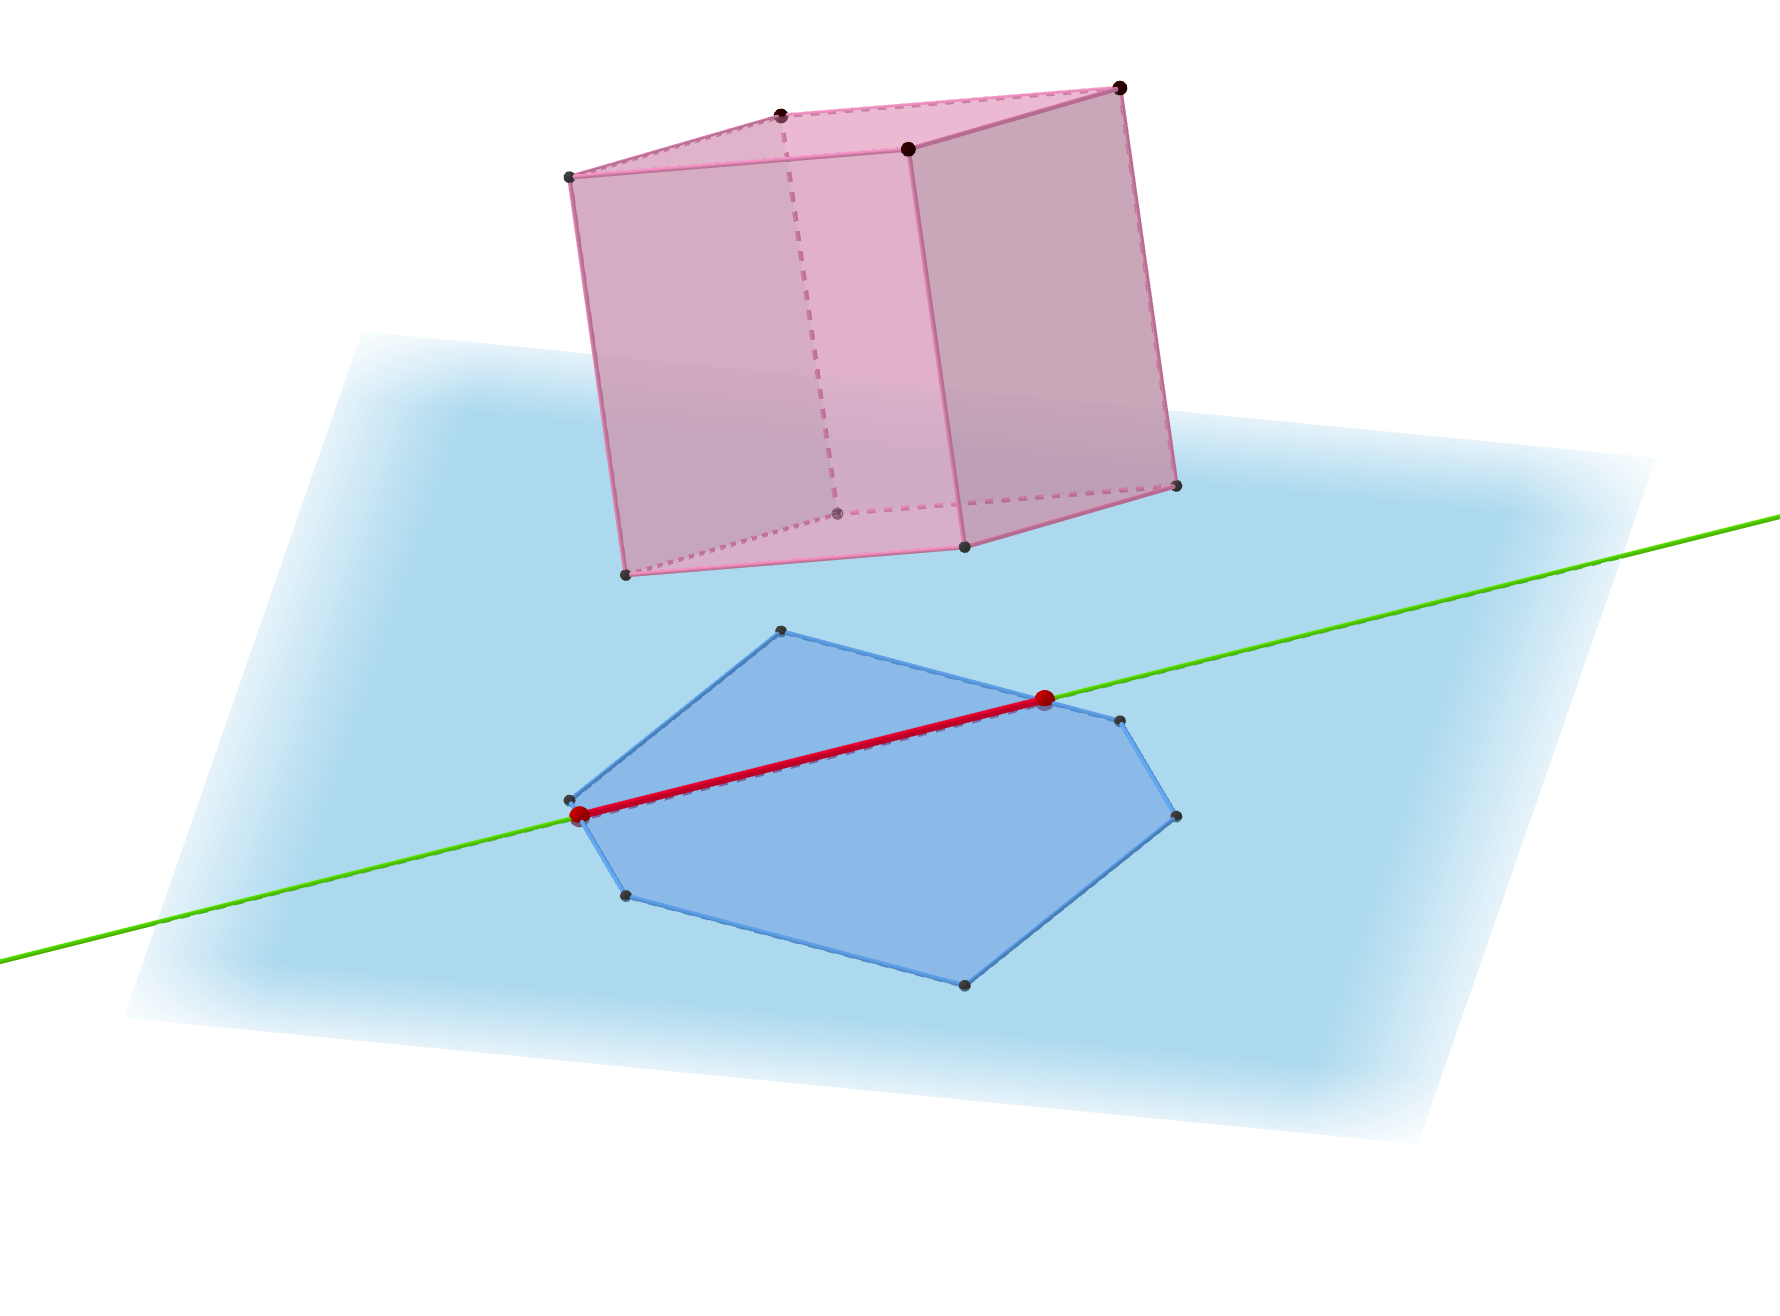
\includegraphics[trim={50 150 50 70}, clip, width=1\linewidth]{img/chapter_3/polytope_better_ggb.png}
    \end{minipage}
    \hfill
    \begin{minipage}{0.48\linewidth}
        \captionsetup{justification=centering}
        \centering
        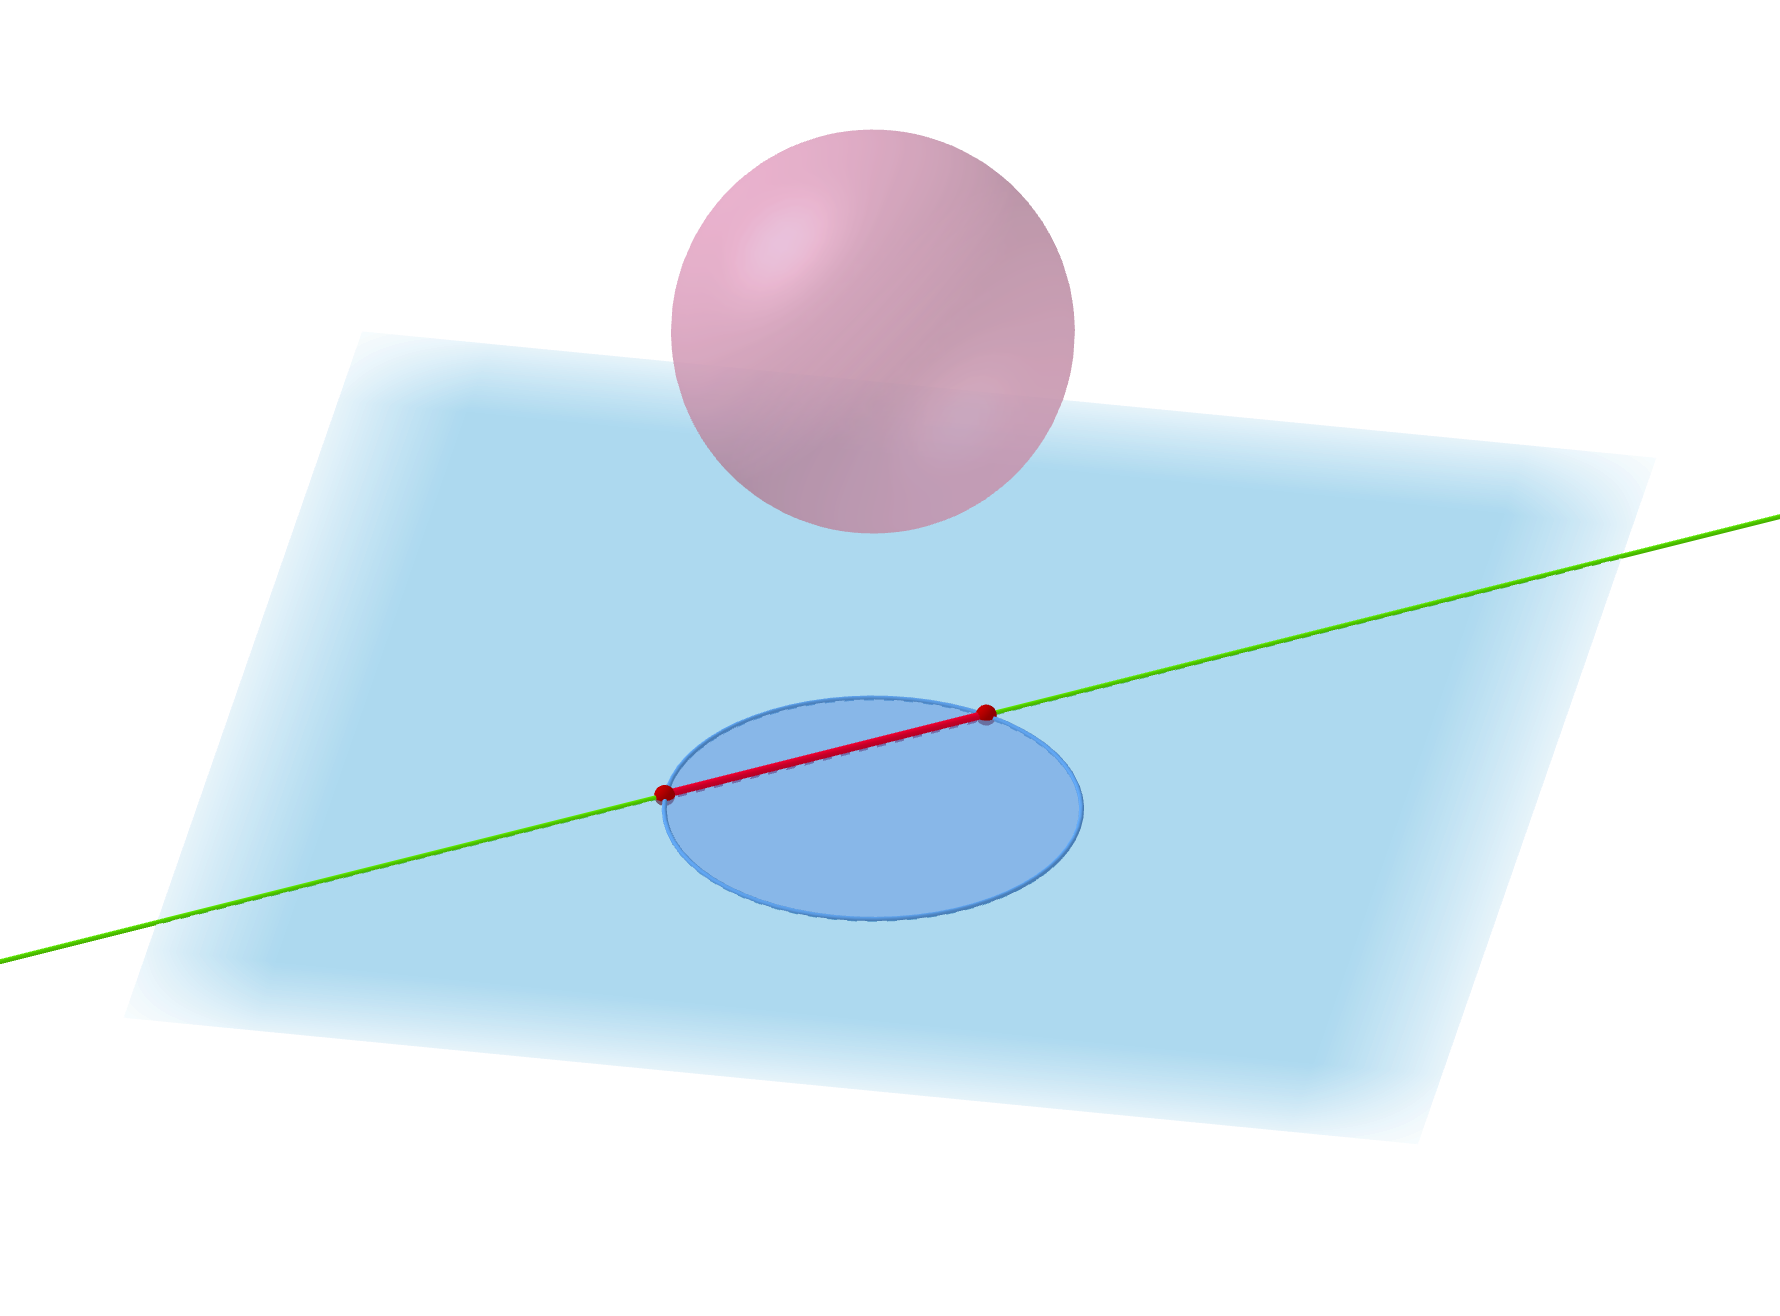
\includegraphics[trim={50 150 50 70}, clip, width=1\linewidth]{img/chapter_3/polytope_from_sphere_ggb.png}
    \end{minipage}
    \caption{Force feasible set $\mathcal{F}$ (red) resulting from different tension feasible sets $\mathcal{T}$ (pink). The blue shape represents the torque feasible set, and the green line represents $\im{J^T}$.}
    \label{fig:tension_models_on_ffs}
\end{figure}

We will now detail how to explicitly compute force feasible sets for both polytopic and ellipsoidal constructions.

\subsubsection*{Representing force polytopes}
When the tension feasible set $\mathcal{T}$ is an orthotope (a generalization of a rectangle to higher dimensions), the force feasible set $\mathcal{F}$ is a \emph{force polytope}. Polytopes have two main distinct representations: the $\mathcal{V}$-representation, which describes the polytope by its vertices, and the $\mathcal{H}$-representation, which describes it by its supporting hyperplanes.

The $\mathcal{V}$-representation of a polytope consists of its extremal points, commonly known as \emph{vertices}. Any point that can be expressed as a weighted average of these vertices is necessarily included in the polytope, as stated by Caratheodory's theorem (\cite{caratheodoryUberVariabilitatsbereichFourierschen1911}). The set of all possible weighted averages of two or more vertices is called the \emph{convex hull} of those vertices. In contrast, the $\mathcal{H}$-representation describes a polytope as the intersection of multiple half-spaces. Each half-space is defined by a linear inequality. Therefore, the $\mathcal{H}$-representation essentially consists of a set of linear inequalities that define the polytope's faces and determine which side of each face belongs to the polytope. Specifically, each face of a polytope can be represented by a \emph{hyperplane} (\cite{grunbaumConvexPolytopes2013}), which is an $(n-1$)-dimensional subspace of an $n$-dimensional space. Figure \ref{fig:polytope_v_and_h_rep} presents simple 2D examples of both representations.
\begin{figure}[!htb]
    \captionsetup{justification=centering}
    \begin{minipage}{0.49\linewidth}
        \centering
        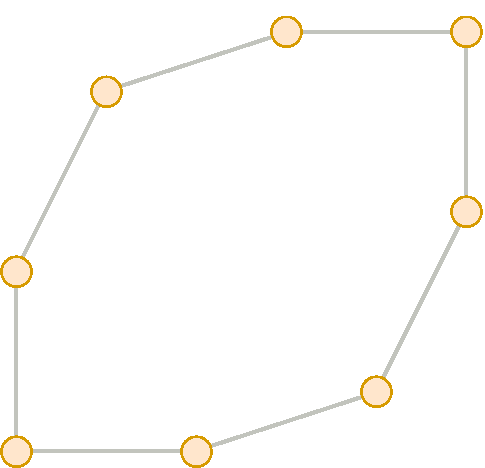
\includegraphics[trim={0 0 0 0},clip, width=0.6\linewidth]{img/chapter_2/zonotope_vertices.pdf}
    \end{minipage}
    \hfill
    \begin{minipage}{0.49\linewidth}
        \centering
        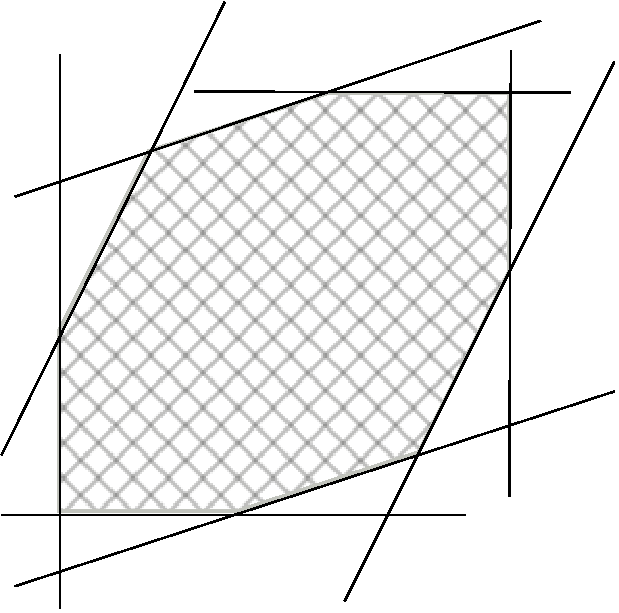
\includegraphics[trim={0 0 0 0},clip,width=0.75\linewidth]{img/chapter_2/zonotope_hyperplanes.pdf}
    \end{minipage}
    \caption{Polytope representations: A polytope can be described according to its vertices (the $\mathcal{V}$-representation) or by halfspaces determined from its bounding hyperplanes (the $\mathcal{H}$-representation).}
    \label{fig:polytope_v_and_h_rep}
\end{figure}

The $\mathcal{V}$- and $\mathcal{H}$-representations are equivalent when a polytope is \emph{full-dimensional} (\cite{grunbaumConvexPolytopes2013}), meaning it has the same dimension as the \emph{ambient} space. An ambient space refers to the surrounding space in which the polytope is described. When a polytope is full-dimensional, this is equivalent to saying that the polytope is not \emph{flat} in the ambient space. For instance, a polygon in a 3D space is not full-dimensional and is considered \emph{degenerate}. Force polytopes, when expressed in the torque space, are often degenerate, specifically when the rank of $\im{J^T}$ is strictly less than the dimension of the torque space, as shown in figure \ref{fig:ffs_when_tension_set_orthotope}.
\begin{figure}[!htb]
    \captionsetup{justification=centering}
    \centering
    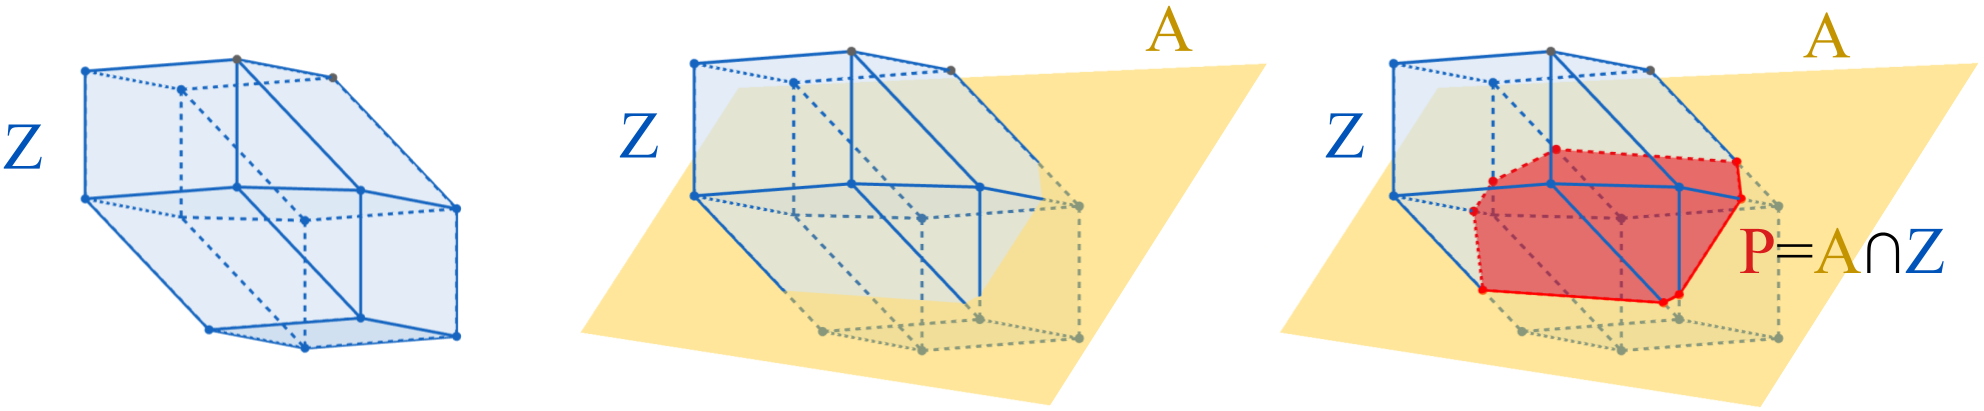
\includegraphics[trim={0 0 0 0}, clip, width=1\linewidth]{img/chapter_1/Polytope inter.png}
    \caption{Construction of a force polytope $P$ from a tension orthotope $\mathcal{T}$. $\mathcal{T}$ is projected onto the 3D torque space ($Z$), then intersected with the 2D subspace $\im{J^T}$ ($A$). The resulting force polytope P is degenerate as it is 2-dimensional within the 3D ambient torque space.}
    \label{fig:ffs_when_tension_set_orthotope}
\end{figure}

The $\mathcal{V}$- and $\mathcal{H}$-representations are the most common, as they encapsulate crucial information that force polytope construction does not share at first sight: they characterize a polytope's \emph{surface}. So, in order to visualize a 3D force polytope, a correspondence from the projection-intersection description should be made to either its vertices or bounding hyperplanes. Either representation would suffice, as algorithms already exist to convert from the $\mathcal{V}$- to the $\mathcal{H}$-representation, as described in (\cite{avisPivotingAlgorithmConvex}).

One approach is to explicitly compute the $\mathcal{H}$-representation of the torque feasible set, which is the projection of the tension feasible orthotope onto the torque space. Numerous algorithms exist for this purpose, such as the \emph{Hyperplane-Shifting method} (\cite{gouttefardeCharacterizationParallelManipulator2010a}) for describing the bounding hyperplanes, or the algorithms proposed in (\cite{radaNewAlgorithmEnumeration2018}) and (\cite{guCounterfactualIdentificationLatent2022}) for enumerating the vertices. Next, we need to compute the polytope that results from intersecting this torque feasible set with $\im{J^T}$. Once we have the bounding hyperplanes of the torque feasible set, we intersect each of them with $\im{J^T}$. This creates a new set of half-spaces within $\im{J^T}$. The force polytope is then defined as the smallest polytope enclosed by these new half-spaces. The Fourier-Motzkin elimination method can be used to obtain this new set of half-spaces, as it is specifically designed to find the smallest polytope enclosed by a given set of hyperplanes (\cite{dahlCombinatorialPropertiesFourierMotzkin2007}).

Although this direct approach is theoretically feasible, it is often impractical due to the high computational cost. Most algorithms for computing the $\mathcal{V}$-representation or $\mathcal{H}$-representation of polytopes are combinatorially complex, meaning their time complexity increases exponentially with the dimension of the muscle tension space. In Chapter \ref{chapter:2}, we will further demonstrate this computational challenge by benchmarking various algorithms for projecting the tension orthotope onto the torque space. We will also propose a new edge-based algorithm for efficiently describing the surface of the torque feasible set, leveraging its representation as a projection of an orthotope. Even with efficient algorithms, any exact description of the torque feasible set's surface will inevitably suffer from combinatorial complexity. Therefore, to avoid this computational bottleneck, approximation algorithms are often preferred for computing points on the polytope's surface. One such example is the \emph{Iterative Convex Hull} method proposed in (\cite{skuricOnLineFeasibleWrench2022}).

Beyond the $\mathcal{V}$- and $\mathcal{H}$-representations, there are many other possible polytope representations that capture specific polytope properties, just as the $\mathcal{V}$- and $\mathcal{H}$-representations encapsulate surface properties. For example, the \emph{Ehrhart quasi-polynomial} of a polytope $P$ is a polynomial of a positive variable $t$ that counts the number of integer points within a dilation $tP$ of the polytope. However, computing the coefficients of these polynomials is computationally expensive, with the combinatorial complexity increasing significantly as the number of vertices and the dimension of the polytope increase (\cite{barvinokComputingEhrhartQuasipolynomial2005}). A more practical representation is the \emph{constrained zonotope} representation, introduced in (\cite{scottConstrainedZonotopesNew2016}). The authors showed that any polytope can be constructed by intersecting a hypercube with a linear subspace and then projecting the result onto another subspace. Although this result was previously proven in (\cite{naumannBeliebigeKonvexePolytope1956}) and discussed by Grünbaum in (\cite{grunbaumConvexPolytopes2013}), it remains largely theoretical, with no explicit construction method provided. In Chapter \ref{chapter:3}, we leverage this result by demonstrating how to transform the projection-intersection description of a polytope (as we have enunciated for force polytopes) into an intersection-projection description. We provide an explicit method for this transformation. Our result is quite general, as it applies to any convex set constructed in this way, including arbitrary force feasible sets derived from convex tension feasible sets. The primary goal of this geometric inversion is to re-express linear constraints in the torque space as linear constraints in the muscle tension space. This is useful for geometrically identifying the muscles that are primarily responsible for generating forces at the end-effector.

\subsubsection*{Representing force ellipsoids}
A \emph{force ellipsoid} is a force feasible set that results from assuming the tension feasible set is an ellipsoid. This provides an alternative representation of force feasible sets, as demonstrated in (\cite{chiacchioForcePolytopeForce1997}), who used it to characterize the manipulability of a serial robot. In the context of biomechanics, this representation implies that the tension a muscle can exert depends on the tensions of all other muscles in the system. Specifically, the vector of muscle tensions must lie within an ellipsoid in the muscle tension space.

Whereas characterizing the surface of force polytopes is computationally challenging, force ellipsoids are much easier to compute and do not involve combinatorial complexity. This simplicity stems from the fact that both projections and intersections of ellipsoids with vector spaces result in ellipsoids (\cite{grunbaumConvexPolytopes2013}).

Any ellipsoid can be represented as an affine transformation of a unit sphere. Let $\mathcal{E}$ be an ellipsoid in $\IR^m$ and let $\mathcal{S}$ denote the unit sphere in $\IR^m$. Then, there exists a matrix $T\in\IR^{m\times m}$ and a vector $\mathbf{t}\in\IR^m$ such that:
\begin{align*}
    \mathcal{E} = T\mathcal{S} + \mathbf{t} = \left\{ \mathbf{x}\in\IR^m \mid \mathbf{x} = T\mathbf{u} + \mathbf{t}, \quad \|\mathbf{u}\|_2 = 1 \right\}
\end{align*}
where $\| \cdot \|_2$ denotes the usual Euclidean norm in $\IR^m$. 

Any linear transformation $T$ can be decomposed into three parts: 1) a rotation; 2) an \emph{anisotropic dilation}, which scales the sphere by different factors along its principal axes; 3) another rotation. This is known as the \emph{singular value decomposition} (SVD) of a linear transformation. The SVD provides a geometric interpretation of how the linear transformation $T$ deforms a unit sphere. Recall that the torque feasible set is obtained by projecting the tension ellipsoid onto the torque space. Since the projection is a linear transformation, and the composition of linear transformations is another linear transformation, the resulting torque feasible set is also an ellipsoid. However, the intersection of an ellipsoid with a vector space requires a more involved computation. In (\cite{sasakiHigherDimensionalSpatial2010a}), the authors offer a mathematical method to compute such an intersection.

Both the projection and intersection operations involve only matrix operations and vector translations. Therefore, force ellipsoids offer a significant computational advantage over force polytopes, which require addressing combinatorial problems.

\subsection{Conclusion}
In this section, we first described how a human upper limb can be represented \emph{in silico} using a model of a serial kinematic chain and muscles. This model allowed us to analyze the dynamics of the upper limb, which are captured by the \emph{equation of motion}. This equation relates the generalized coordinates, their velocities, and accelerations within the torque space. We considered both internal and external forces acting on the system. The internal forces are the muscle forces, and the external forces are those applied at the end-effector (the hand). We then expressed these forces in the torque space to incorporate them into the equation of motion. This led to the mathematical definition of the \emph{force feasible set} as the set of all external forces that can be applied at the end-effector while satisfying the equation of motion.

To analyze the force capabilities of the upper limb in static postures, we focused on force feasible sets in \emph{isometric} conditions, where the generalized velocities and accelerations are zero, and the musculotendon units are in equilibrium, meaning there is no movement. This allows for a more succinct representation of the force feasible sets, as the terms related to mass inertia and Coriolis accelerations in the equation of motion can be eliminated. We also presented a geometric interpretation of force feasible sets, highlighting their construction through a linear projection followed by an intersection with a vector space. These two operations are fundamental in set theory and have been extensively studied in the literature (\cite{bourbakiTheorieEnsembles2006}; \cite{dorstGeometricAlgebraComputer2007}).

However, even when assuming that the geometric construction of the force feasible sets depends only on convex sets - which is advantageous since a convex set is fully determined by its surface - we observed that the process of projecting and then intersecting introduces significant complexity in characterizing the surface of the resulting set. As examples, two common force feasible set representations were compared in terms of computing difficulties: force polytopes and force ellipsoids. Both characterization as polytopes and ellipsoids have been extensively studied in the literature (\cite{grunbaumConvexPolytopes2013}; \cite{artstein-avidanAsymptoticGeometricAnalysis2015}), and the projection-intersection problem is well-understood for both cases. However, the ellipsoid representation offers a significant computational advantage, as it involves only linear algebra operations.

It is important to consider other geometric characterizations of force feasible sets because, as we will see in Section \ref{sec:modeling_muscle_tensions}, the polytope and ellipsoid approaches have limitations in capturing the complex interactions between muscle tensions. Modeling the interactions between muscle tensions leads to a specific shape for the tension feasible set, which in turn influences the shape of the force feasible set. Chapter \ref{chapter:3} is dedicated to this problem, specifically addressing the case of a complex upper-limb muscular structure with a high number of muscles. In Chapter \ref{chapter:3}, we will show that for a complex musculoskeletal model, force polytope and ellipsoid representations are likely to be equivalent up to dilation. This means that the shape of any force feasible set is essentially the same ellipsoid but with a different scale, provided the muscle tension feasible set is convex and of sufficiently high dimension. While this theoretical result assumes a sufficiently large dimension for the muscle tension space, one of the objectives in Chapter \ref{chapter:4} will be to quantify how ellipsoid representations can be equivalent to polytopes in a muscle personalization process, even when only 50 muscles are considered, as the upper-limb musculoskeletal model in (\cite{holzbaurModelUpperExtremity2005}).

In the next section, we will explore the limitations of different force feasible set representations in a biomechanical context, comparing them to measured maximal isometric forces.

\section{Modeling force feasible sets via maximal isometric force measurements}
\label{sec:modeling_muscle_tensions}

As demonstrated by force polytopes and ellipsoids, the shape of a force feasible set is influenced by the shape of the tension feasible set. This section examines the underlying geometric assumptions about tension and torque feasible sets found in the literature and explores how these assumptions translate into biomechanical considerations for the muscles.

This section highlights how the limited diversity of tension interaction models hinders the accurate modeling of force feasible sets in the human upper limb. This limitation arises from the computational challenges involved in considering different tension feasible set shapes. Cable-driven parallel robots, which form the basis of musculoskeletal models, are not necessarily limited by modeling constraints, as their force feasible sets can be arbitrarily defined. However, in a human upper-limb, experimental measurements of maximal isometric force exertions reveal inconsistencies with current force feasible set representations. Specifically, force ellipsoids tend to underestimate the measured forces, while force polytopes tend to overestimate them (\cite{rezzougUpperLimbIsometricForce2021b}).

To examine these disagreements, subsection \ref{subsec:ffs_in_human_upper_limb} details the experimental process required for measuring maximal isometric force exertions, while subsection \ref{subsec:force_measurements_vs_ffs} discusses how \emph{in silico} force capabilities are adapted to agree with \emph{in vivo} force measurements.

\subsection{\emph{In vivo} measurements of force feasible sets in the human upper-limb}
\label{subsec:ffs_in_human_upper_limb}
Convex force feasible sets in isometric conditions can be characterized by the set of all maximal forces on their surfaces. Since there are infinitely many such maximal forces, experimental measurement presents inherent challenges. This subsection first focuses in \ref{subsec:mvic} on measuring a maximal force in an individual, detailing the various factors that must be considered to ensure accurate measurement. Then, subsection \ref{subsec:reconstruction_from_mvic} discusses how current in silico representations are limited in their ability to accurately capture these measurements. This highlights the need for more sophisticated force feasible set models that can better represent the complexities of human force capabilities.

\subsubsection*{Maximal voluntary isometric contraction (MVIC)}
\label{subsec:mvic}

Measuring isometric force exertion requires a demanding experimental procedure, particularly because force exertions are linked to musculoskeletal disorders (\cite{hoozemansPushingPullingRelation1998}; \cite{hoozemansMechanicalLoadingLow2004}). This protocol, known as \emph{maximal voluntary isometric contraction} (MVIC), measures an individual's maximal force exertion and provides a simple method of assessing muscle strength (\cite{meldrumMaximumVoluntaryIsometric2007}). MVIC is typically measured using a dynamometer (\cite{robertsReviewMeasurementGrip2011}) or a force/torque sensor, which allows for the evaluation of the produced force and/or torque. The peak force generated during an isometric contraction against the sensor is recorded as the MVIC. The duration of the MVIC recording can vary depending on the specific research question.

Several factors can influence MVIC measurements. These include the individual's posture (\cite{watanabeShortTermReliabilityGrip2005}; \cite{robertsReviewMeasurementGrip2011}) and gender (\cite{vanderbeekGenderDifferencesExerted2000}; \cite{robertsReviewMeasurementGrip2011}), as well as the direction of force exertion and their hand dominance (\cite{jansenEffectsFingernailLength2000}). Other influencing factors include the individual's respiration conditions (\cite{leeComparisonMaximumVoluntary2016}) and medical condition, the number of repeated MVIC measurements (\cite{watanabeShortTermReliabilityGrip2005}; \cite{robertsReviewMeasurementGrip2011}), the exertion time (\cite{roseFatigueRecoveryStatic2014}), the shape of the handle used for force exertion, the muscle resting time (\cite{watanabeShortTermReliabilityGrip2005}), and the perceived resting time required before another exertion (\cite{roseFatigueRecoveryStatic2014}).

% Force feasible sets, as we described in section \ref{sec:muscu_model_in_silico_ffs}, encompasses some of these factors in their general definition such as the influence of the posture and the direction of the exerted force.

The following studies present experimental protocols for force measurements. While measuring a maximal voluntary isometric force in a specific direction may not be the primary objective of all the studies, they show how a force exertion can be influenced by various factors. However, all of these studies involve the measurement of forces exerted at the hand.

\paragraph*{Hand dominance.} Studies on hand dominance and grip strength have shown that right-handed individuals have a grip that is approximately 10\% stronger in their dominant hand compared to their non-dominant hand (\cite{jansenEffectsFingernailLength2000}; \cite{bohannonGripStrengthSummary2003}). However, this trend is not observed in left-handed individuals, whose grip strength tends to be equal in both hands (\cite{crosbyHandStrengthNormative1994}; \cite{bohannonGripStrengthSummary2003}). Consequently, hand dominance is an important factor to consider when measuring maximal isometric forces at the right hand.

\paragraph*{Respiration.} In (\cite{leeComparisonMaximumVoluntary2016}), the authors showed that respiration conditions can also influence MVIC measurements at the hand. The study involved 13 males and 9 females (age $22.6\pm 2.4$ years old). The MVIC was measured in a standing posture with the elbow flexed at 90°. The results showed that, on average, the MVIC was significantly higher during expiration after a maximal inspiration compared to inspiration after a maximal expiration. Based on these findings, the authors recommend keeping the same respiration method for all MVIC measurements to ensure consistency.

\paragraph*{Perceived fatigue.} Furthermore, (\cite{roseFatigueRecoveryStatic2014}) demonstrated the influence of perceived fatigue on force exertion. The study showed that the required resting time between two trials of a task involving pushing a load (a static handle at shoulder height) increases exponentially with both the amount of force produced and the duration of the exertion. The specific exponential curve varies between individuals. For example, one male participant who pushed the handle for 30 seconds at 50\% of his MVC needed at least 2 minutes of rest before the next trial. However, the study had limitations, including a small number of trials per participant (only 2) and a focus on long exertions. Despite these limitations, the study suggests a relationship between achieving a MVIC and the individual's resting time.

\paragraph*{Body posture.} The authors in (\cite{watanabeShortTermReliabilityGrip2005}) conducted a study to investigate the short-term reliability of hand grip strength in different postures, with a focus on shorter exertion times. The study involved 100 healthy subjects (50 male and 50 female, mean age 38.2 years old) who performed maximal grip exertions on a handle. The exertions were performed with and without the use of the non-dominant hand, repeated three times with and without 1-minute resting intervals, and conducted in three different body positions: standing, sitting, and supine. The main finding of the study was that 1-minute resting intervals were sufficient to maintain a consistent maximal grip force across the three trials. However, the study did not specify the duration of the grip exertion, stating only that it was short and varied between participants. The results also showed no significant difference in grip strength between the standing and sitting postures, but a significant difference was observed for the supine posture.

\paragraph*{Circadian rythm.} It is also important to note that the time of day can also influence MVIC. (\cite{jasperCircadianVariationsKinematics2009}) showed that maximum hand grip strength exhibited a circadian rhythm, with the lowest strength values observed at 06:00h and the highest at 18:00h. This difference was significant regardless of whether the subjects were sleep-deprived.

\paragraph*{Encouragements.} Also, it was shown in (\cite{jungEffectsInstructionVerbal1999}) that both visual and verbal encouragement can influence MVIC measurements. Their study examined these effects on the handgrip strength of 16 male subjects (age $27\pm 3.72$). Providing verbal encouragement by continuously shouting `Go' resulted in a significantly higher peak force. Similarly, providing visual feedback, where subjects could see their force output in real time, also led to significantly better results. In another study (\cite{johanssonRelationshipVerbalCommand1983a}), the authors investigated the effect of the volume of MVIC instructions on the resulting MVIC at the hand for the triceps brachii muscle. The measurements were taken in a supine position with the right shoulder at 90° of abduction and the elbow at 90°. Their findings showed that providing instructions at a loud conversation level (88 dBA) resulted in significantly greater muscle force compared to a soft conversation level (66 dBA). Furthermore, a set of standardized instructions was defined in (\cite{mathiowetzReliabilityValidityGrip1984a}) to ensure consistency in maximal grip strength measurements over three trials. This suggests that verbal encouragement can help improve the quality of MVIC measurements.

While these studies highlight the various factors that can influence MVIC measurements, accurately characterizing the surface of a force feasible set in a given posture theoretically requires measuring an infinite number of MVICs. Since this is not practically feasible, the next paragraphs will examine current protocols used to collect a sufficient number of MVIC measurements to approximate a force feasible set.

\subsubsection*{Reconstructing a force feasible set from MVIC measurements}
\label{subsec:reconstruction_from_mvic}
The following studies involve the collection of multiple maximal voluntary isometric contractions. These studies share some common features: all measurements involved forces exerted at the hand with the right upper limb in one or more fixed postures. Since there is no standard protocol for selecting force directions, the following studies employ different methods for choosing them.

\paragraph*{Posture stabilization.} To ensure accurate measurement of multiple maximal voluntary isometric contractions in isometric conditions, the participant's posture must be fixed. Participants typically adopt a sitting posture, and only their upper-limb posture is adjusted to achieve different configurations. One challenge is to stabilize the participant's trunk to isolate the upper-limb movements. Several studies have used two belts to secure the trunk against a chair, thereby minimizing the influence of upper body movements (\cite{oshimaRoboticAnalysesOutput2000}; \cite{sasakiHigherDimensionalSpatial2010a}; \cite{hernandezHumanUpperlimbForce2016a}; \cite{rezzougUpperLimbIsometricForce2021b}).

\paragraph*{Isolation of upper-limb forces.} A major challenge in measuring forces exerted by the upper-limb muscles is ensuring that no other forces are exerted, both from within the upper limb itself and from the rest of the body. Contact forces are inherent to a sitting posture and therefore unavoidable. However, other forces, such as those arising from ground contact with the feet, should be minimized. In (\cite{leeBiomechanicalAnalysisCoordinated2023}), a significant correlation between ground contact forces and hand contact forces produced simultaneously was noticed. Specifically, the authors found a relationship between the minimum ground contact forces and the maximum hand forces produced. Although this study focused on a standing posture, it suggests the importance of minimizing foot contact forces to ensure accurate measurement of maximal hand force exertion.

\paragraph*{Posture determination.} To prevent external forces from being exerted on the upper limb during MVIC measurements, contact forces over the upper limb itself should also be minimized. This means that the upper limb should not be constrained by belts or any other mechanical system used to maintain a specific posture. Consequently, since the posture is not constrained, it must be determined directly from the subject. In (\cite{rezzougUpperLimbIsometricForce2021b}) and (\cite{hernandezHumanUpperlimbForce2016a}), an optoelectronic system was used with reflective markers placed on the upper limb according to the recommendations of the International Society of Biomechanics (\cite{wuISBRecommendationDefinitions2005}; \cite{senkRotationSequenceImportant2006a}) (see Figure \ref{fig:hernandez_opto}). This system uses multiple cameras to track the 3D positions of the markers. The marker placement allows us to scale a generic musculoskeletal model to the subject by adjusting the bone lengths to match the marker positions. Inverse kinematics can then be applied to the scaled model to determine the individual's posture, as described in (\cite{luBonePositionEstimation1999}) and (\cite{rouxEvaluationGlobalOptimisation2002}).
\begin{figure}[!htb]
    \captionsetup{justification=centering}
        \centering
        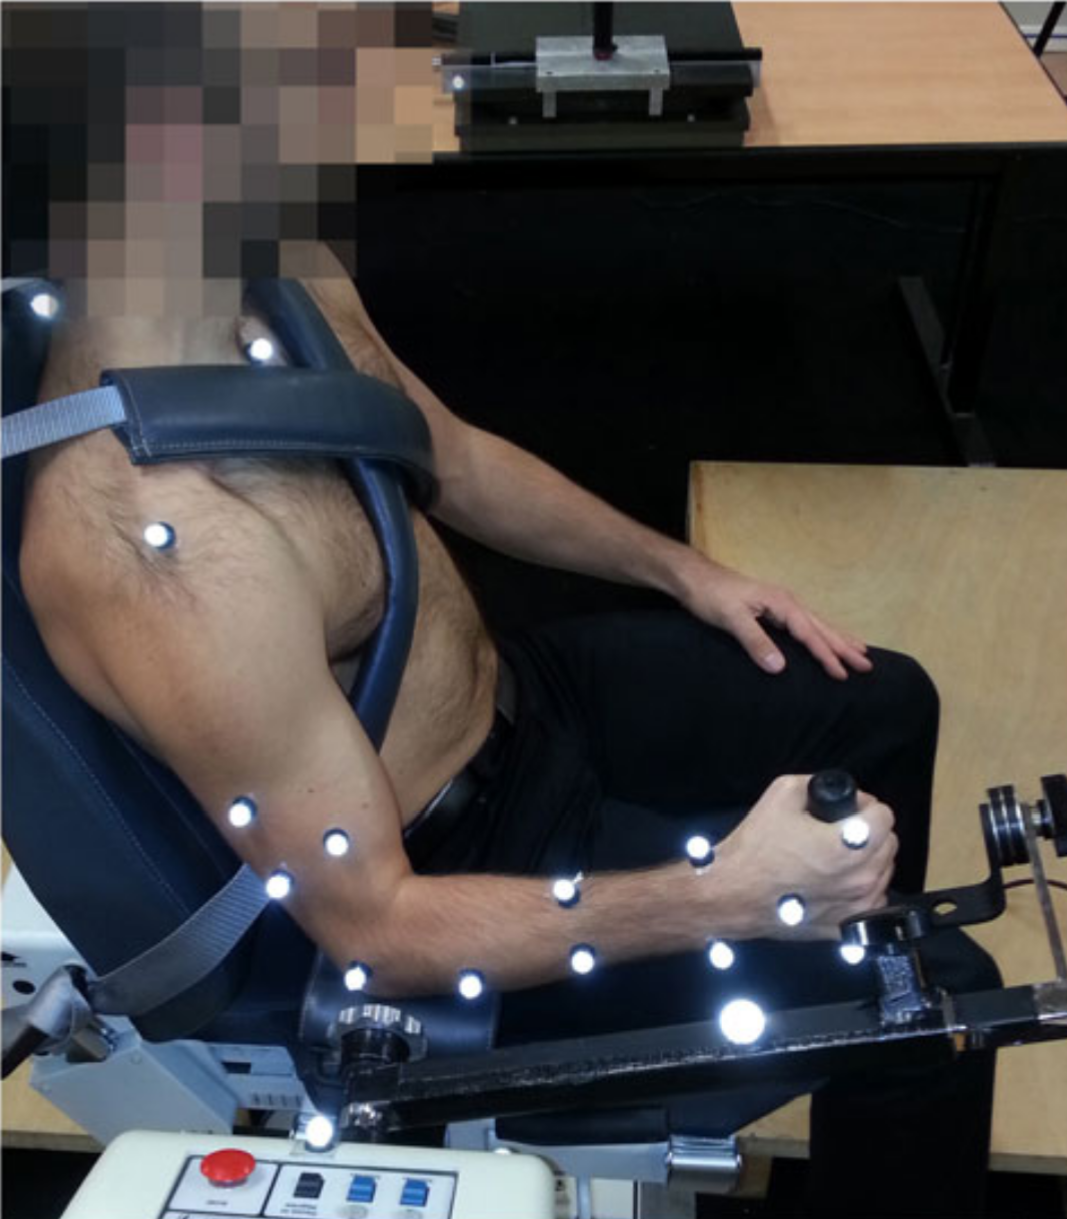
\includegraphics[trim={0 0 0 0},clip,width=0.4\linewidth]{img/chapter_1/hernandez_optoelectronic.png}
    \caption{Reflective markers placed on the upper-limb (\cite{hernandezHumanUpperlimbForce2016a}).}
    \label{fig:hernandez_opto}
\end{figure}

\paragraph*{Force directions.} The choice of directions for exerting MVICs varies depending on the posture and the desired range of force directions (a line, a plane, or the entire 3D space). 

While predicting force amplitude in a specific direction is of strong interest for characterizing individual force capabilities, this thesis focuses on understanding the underlying muscle tension interactions that generate these forces. Previous studies have explored various approaches for predicting maximal force exertion in regard to a specific direction, such as using artificial neural networks to relate upper-limb posture and anthropometric data (\cite{ladelfaArmForceField2017a}; \cite{ladelfaPredictingManualArm2016b}) or employing parametric equations to predict maximum hand force based on hand location relative to the shoulder (\cite{ladelfaEquationsPredictFemale2014a}). However, these studies do not seek to characterize how muscle tensions interact to produce these forces. As this thesis will focus this characterization, we do not expand on the predicting aspect of maximal force exertion and focus on the chosen directions within experimental procedures. 

As experimentally observed in (\cite{jannijhofMaximumIsometricArm2006a}), in which six participants were asked to exerted maximal forces at the hand in eight directions of the workspace in five different hand locations on the transverse plane, the maximum produced forces systematically depended on the hand location and the direction of exertion.

In (\cite{oshimaRoboticAnalysesOutput2000}), the authors investigated forces exerted at the hand in the transverse plane. In this 2D condition, they measured maximal voluntary isometric contractions from four subjects, with exertions performed in various directions within the horizontal plane. Each exertion lasted 1 to 2 seconds, and measurements continued until a sufficient number of directions were sampled. The subjects gripped a horizontal handle, and two postures were considered. However, the authors did not specify whether a resting period was included between measurements or how many directions were considered sufficient. 

In (\cite{sasakiHigherDimensionalSpatial2010a}), 2D force exertions in the transverse plane at the hand were also investigated, using 7 postures and a single participant. A handle was attached to a mechanical mechanism to allow for different wrist postures. In this work, 8 force directions were considered, as described in Figure \ref{fig:sasaki_foce}.
\begin{figure}[!htb]
    \captionsetup{justification=centering}
        \centering
        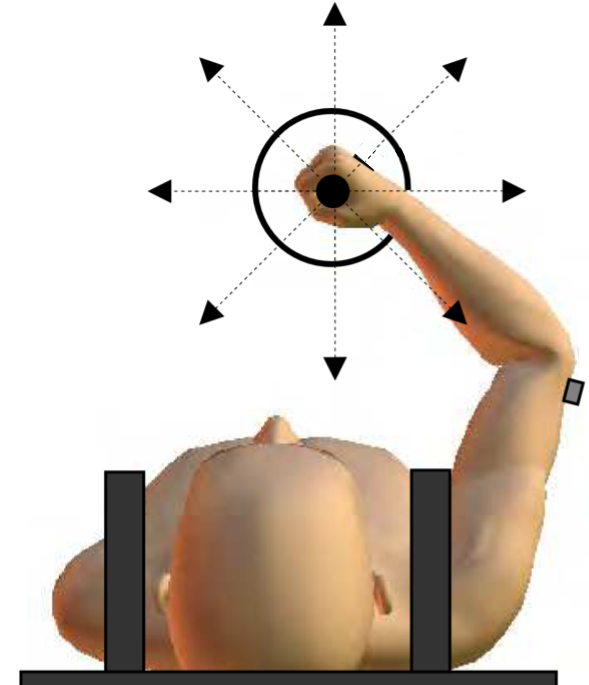
\includegraphics[trim={0 0 0 0},clip,width=0.4\linewidth]{img/chapter_1/sasaki_force.png}
    \caption{Hand force exertion directions used in (\cite{sasakiHigherDimensionalSpatial2010a}).}
    \label{fig:sasaki_foce}
\end{figure}

In contrast to the previous 2D studies, in (\cite{rezzougUpperLimbIsometricForce2021b}) the authors considered seven participants exerting maximal isometric forces in the whole 3D space, using a single posture. This posture involved slight shoulder flexion, an elbow flexed at 70°, and forearm pronation-supination at 80°. Participants exerted maximal isometric forces on a vertical handle attached to a dynamometer in 26 specified directions. These directions were defined as combinations of azimuth angles (ranging from 0° to 315° relative to the horizontal forearm axis in 45° steps) and elevation angles (-45°, 0°, and 45° relative to the horizontal plane). Two additional vertical directions, corresponding to 90° and -90° elevation, were also included. Each maximal force exertion was held for 3 seconds, with a 3-minute resting period between trials.

Similarly, (\cite{hernandezIsometricForceCapabilities2015}) employed a similar protocol, using the same 26 force directions. In their study, participants exerted maximum force for 3 seconds with verbal encouragement. Resting periods lasting 3 minutes were also included between trials.
\begin{figure}[!htb]
    \captionsetup{justification=centering}
        \centering
        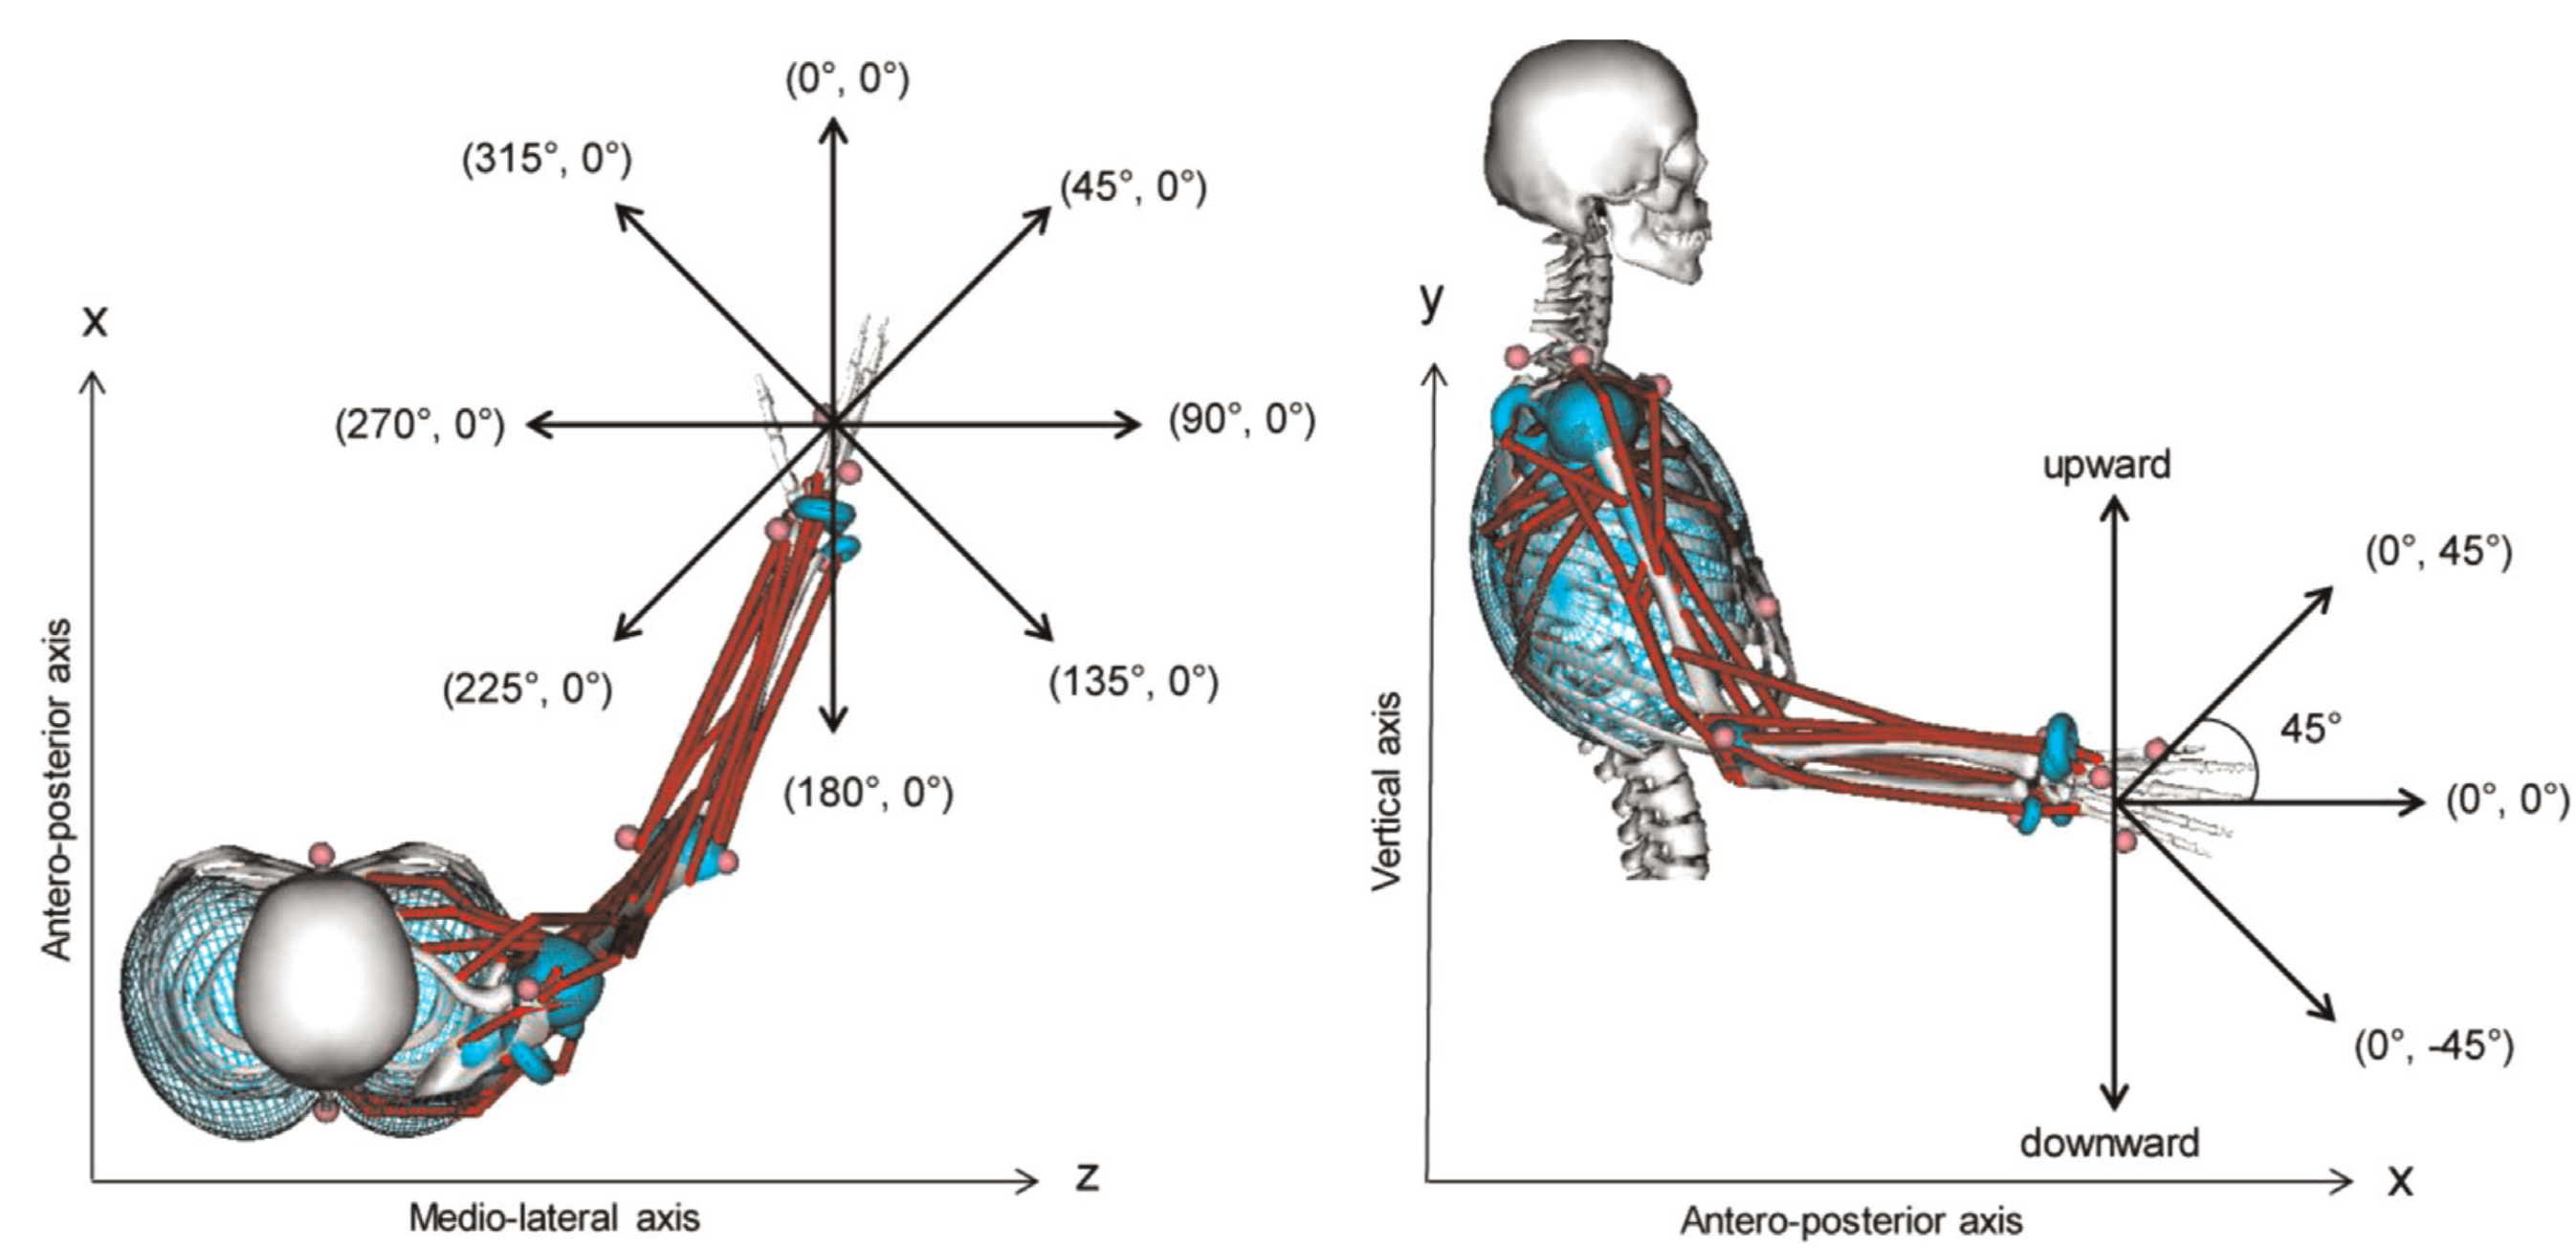
\includegraphics[trim={0 0 0 0},clip,width=1\linewidth]{img/chapter_1/axis_hernandez_rezzoug.png}
    \caption{The 26 force directions used in (\cite{rezzougUpperLimbIsometricForce2021b}) and (\cite{hernandezIsometricForceCapabilities2015}), defined by combinations of azimuth (left figure) and elevation (right figure) angles. Images from (\cite{hernandezIsometricForceCapabilities2015}).}
    \label{fig:rezzoug_hernandez_directions}
\end{figure}

As this review has shown, the inherent challenges of measuring maximal voluntary isometric contractions (MVICs) are reflected in the difficulty of estimating force feasible sets, which require multiple successive MVICs in a given posture. The required resting times between measurements result in lengthy experimental protocols, which become even longer as the number of force directions increases. These challenges may explain why the literature lacks studies with a sufficient number of MVICs measured in a single posture. Furthermore, the number of force directions chosen is often arbitrary, aiming to capture the three-dimensional nature of the Cartesian force space. Consequently, there is a need to improve experimental conditions and to gather more force data in a given posture. This would help in understanding how force capabilities vary across individuals.

This thesis addresses these challenges by making two main contributions. Chapter \ref{chapter:3} will demonstrate that in the human upper limb, the high number of muscles leads to a high probability that force feasible sets resemble ellipsoids. This holds under the sole condition that muscle tension interactions are modeled as convex. Since any 3D ellipsoid can be uniquely determined by 9 arbitrary points on its surface (5 points for a 2D ellipsoid), this result implies that measuring a force feasible set experimentally becomes less challenging. Furthermore, to address the lack of maximal force exertion data in the literature, Chapter \ref{chapter:5} will provide measurements of force feasible sets in four different postures for ten subjects.

% \subsection{\emph{In silico} force feasible set limitations towards \emph{in vivo} measurements}
\subsection{Comparison between \emph{in silico} and \emph{in vivo} force feasible sets}
\label{subsec:force_measurements_vs_ffs}
In experimental protocols where MVICs are gathered in multiple directions, the measured force feasible set is constructed as the convex hull of all measured maximal forces (\cite{oshimaRoboticAnalysesOutput2000}; \cite{rezzougUpperLimbIsometricForce2021b}; \cite{hernandezIsometricForceCapabilities2015}). However, there are examples where a set-theoretic approach is not preferred, and maximal forces are considered individually for each direction (\cite{sasakiHigherDimensionalSpatial2010a}).

Although there is a general framework for defining force feasible sets in static postures, in practice, this framework is often simplified or adapted based on biomechanical assumptions. As highlighted in (\cite{sutjiptoComparisonStrengthProfile2024a}), it is ``unclear which methods best suit modelling and representing limb strength''. We will now examine these assumptions in the context of different force feasible set representations.

In (\cite{chiacchioForcePolytopeForce1997}), the authors considered both the polytopic and ellipsoid representations of force feasible sets for a redundant general manipulator, where the number of degrees of freedom exceeds the dimension of the Cartesian space. The key difference from the general formulation presented in Section \ref{sec:muscu_model_in_silico_ffs} is that their analysis focuses solely on serial kinematic chains, which do not require the consideration of muscle and consequently tension feasible sets. For example, they define the force polytope $\mathcal{P}$ in the torque space as:
\begin{align*}
    \mathcal{P} = \im{J^T} \cap \mathcal{O}_{\tau}
\end{align*}
where $\mathcal{O}_{\tau}$ is an orthotope (hyperrectangle) whose principal axes are aligned with the canonical basis of the torque space. Furthermore, this orthotope is assumed to be centered at the origin. If this specific force polytope construction were generalized to include muscles, it would imply a one-to-one correspondence between muscles and joint torques, with each muscle acting exclusively on a single joint.

Similarly, based on the work of (\cite{yoshikawaManipulabilityRoboticMechanisms1985}), these authors define a force ellipsoid E in the torque space as:
\begin{align*}
    \mathcal{E} = \im{J^T} \cap \mathcal{E}_{\tau}
\end{align*}
where $\mathcal{E}_{\tau}$ is a $n$-dimensional axis-aligned ellipsoid in the torque space. The same interpretation as with $\mathcal{P}$ is possible, implying a one-to-one correspondence between muscles and joint torques if this construction were generalized to include muscles.
\begin{figure}[!htb]
    \captionsetup{justification=centering}
    \begin{minipage}{0.48\linewidth}
        \centering
        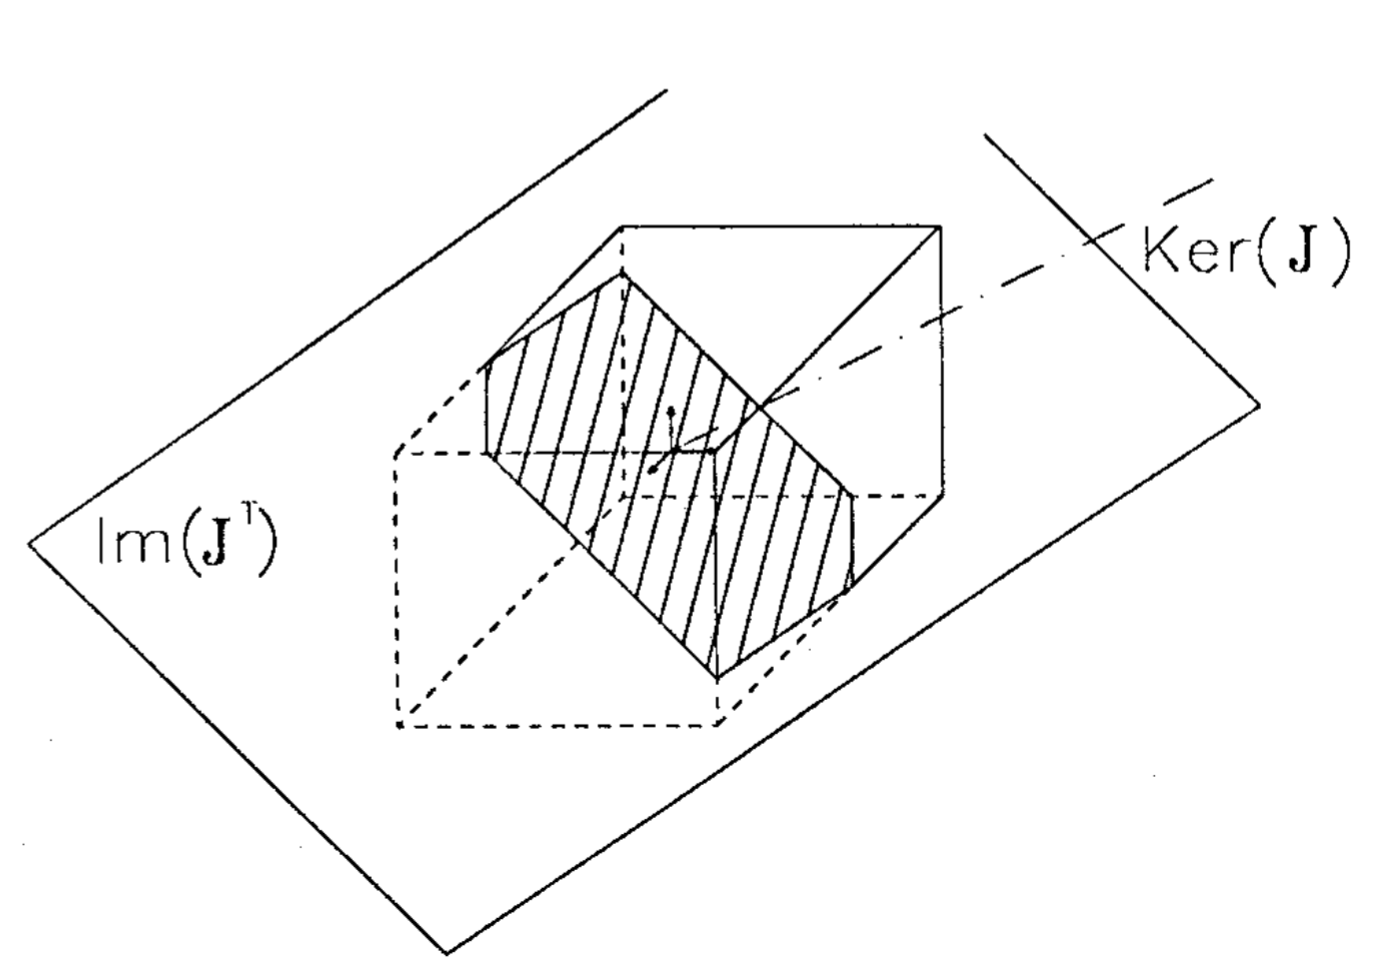
\includegraphics[trim={0 0 0 0}, clip, width=1\linewidth]{img/chapter_1/chiaccho_pol.png}
    \end{minipage}
    \hfill
    \begin{minipage}{0.48\linewidth}
        \centering
        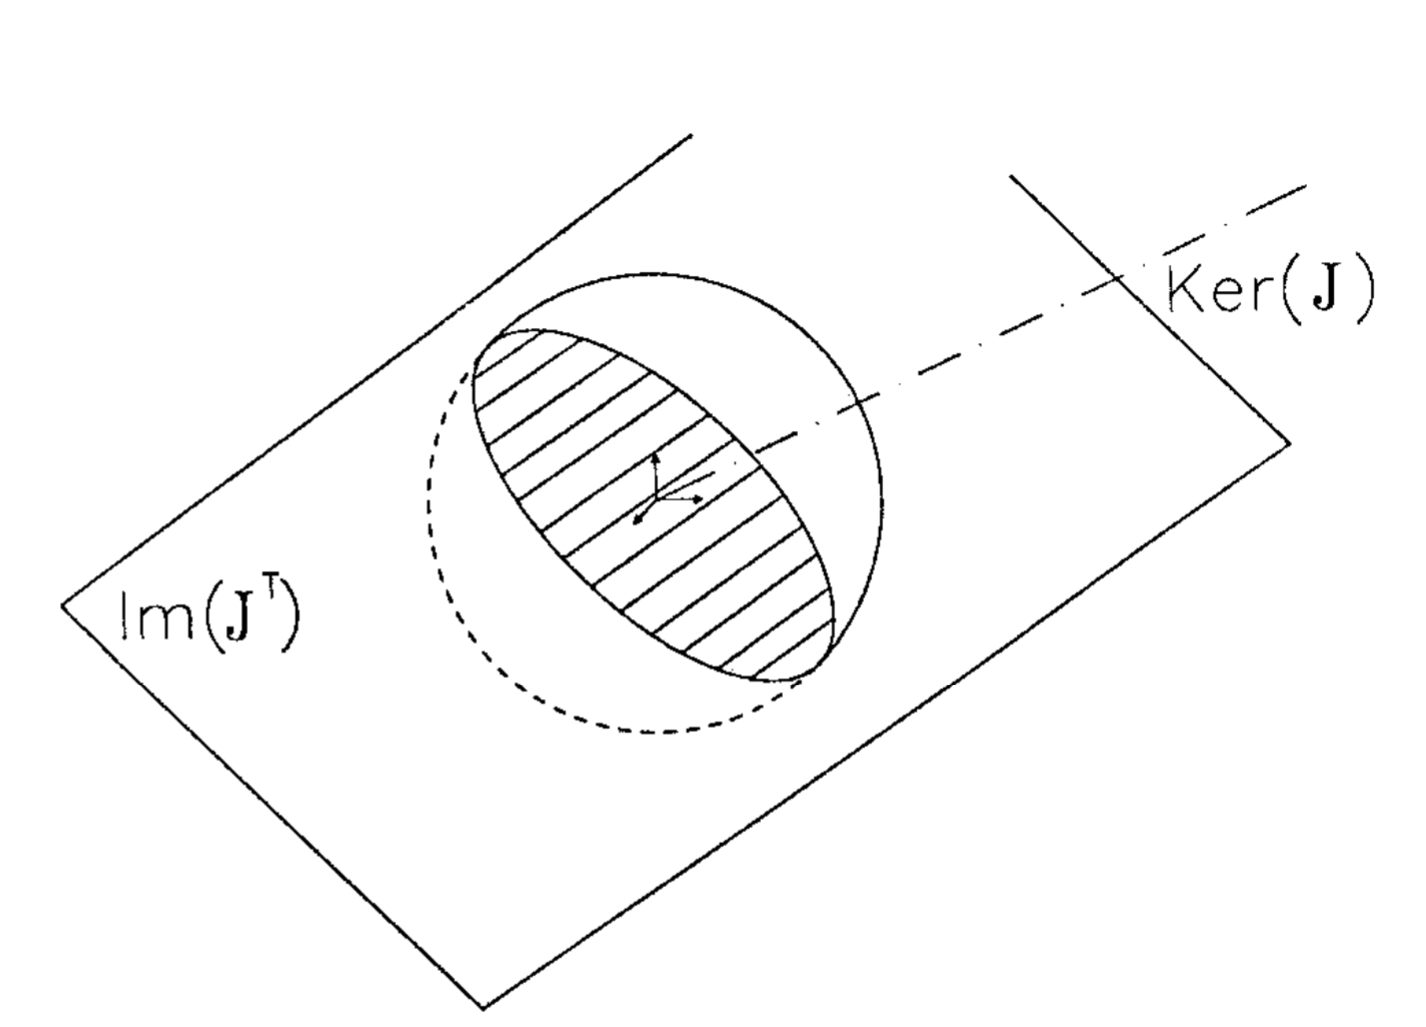
\includegraphics[trim={0 0 0 0}, clip, width=1\linewidth]{img/chapter_1/chiaccho_elli.png}
    \end{minipage}
    \caption{In dashed lines, the force polytope (left) and force ellipsoid (right) construction from (\cite{chiacchioForcePolytopeForce1997}).}
    \label{fig:chiacchio_pol_ell}
\end{figure}

The key difference between these two representations lies in the underlying notion of a norm. In the polytope case, the torque feasible set is an orthotope, obtained by a linear transformation of the unit cube $\mathcal{C} = [-1,1]^n$. This unit cube can be defined as the unit ball $\mathcal{B} = \{\mathbf{x}\in\IR^n \mid \| \mathbf{x} \|_{\infty} \leq 1 \}$ with respect to the infinity norm, where $\|\mathbf{x}\|_{\infty} = \max_i \vert x_i \vert$. Similarly, in the ellipsoid case, the torque feasible set is an ellipsoid, obtained by a linear transformation of the unit ball $\mathcal{B} = \{\mathbf{x}\in\IR^n \mid \| \mathbf{x} \|_{2} \leq 1 \}$ with respect to the Euclidean norm (also termed 2-norm), where $\|\mathbf{x}\|_2 = \sqrt{x_1^2 + \dots + x_n^2}$. Therefore, the different shapes of the force feasible sets in Chiacchio et al.'s work are determined by the choice of norm on the torque space. These norms reflect the degree of independence between the torques. The infinity norm implies complete independence, while the Euclidean norm allows for some interdependence.

Although their representations are specific to pure serial kinematic chains, introducing muscles should lead to different shapes for the torque feasible set. This is primarily because the upper limb has more muscles than degrees of freedom. Therefore, the next example, based on Chiacchio et al.'s construction, investigates the validity of assuming a simpler muscle representation in the upper limb.

(\cite{rezzougUpperLimbIsometricForce2021b}) aimed to demonstrate that the representations proposed by Chiacchio et al., when adjusted based on experimental maximal force and joint torque measurements, do not accurately capture the volume of force feasible sets in the upper limb. They constructed the force feasible set as the convex hull of maximal force measurements taken in 26 directions at the hand. The authors adjusted their \emph{in silico} geometric construction using data from two measurement sessions: one for maximal isometric force exertions at the hand in 26 directions and another for maximal isometric joint torques. Considering 7 degrees of freedom for the upper limb (3 for the shoulder, 1 for the elbow, and 2 for the wrist), they defined the \emph{scaled} force polytope $\mathcal{SP}$ as:
\begin{align*}
    \mathcal{SP} = \im{J^T} \cap \mathcal{O}_{\tau}
\end{align*}
such that $\mathcal{O}_{\tau} = \left([\tau_1^-, \tau_1^+]\times \dots \times [\tau_7^-, \tau_7^+]\right)$ is a 7-dimensional orthotope (hyperrectangle) in the torque space. For each joint $i = 1, \dots, 7$, $\tau_i^- < 0$ represents the maximal measured joint torque in the negative diretion of the joint torque's axis, and $\tau_i^+ > 0$ the maximal joint torque in the positive direction. 

They also defined the \emph{scaled} force ellipsoid $\mathcal{SE}$ as:
\begin{align*}
    \mathcal{SE} = \left(\im{J^T} \cap \mathcal{E}_{\tau}\right) + \overline{\mathbf{f}}
\end{align*}
where $\mathcal{E}_{\tau}$ is the 7 dimensional axis-aligned ellipsoid centered at $0$, with each semi-axis having length $(\vert \tau_i^-\vert + \vert \tau_i^+ \vert)/2$ for $i=1,\dots, 7$. Since there is no reason for $\mathcal{E}_{\tau}$ to be centered at 0 (because $\vert \tau_i^-\vert$ is generally not equal to $\vert \tau_i^+\vert$), the authors compute the intersection $\im{J^T}\cap \mathcal{E}_{\tau}$ and then translate it by an offset $\overline{\mathbf{f}}$. This offset is determined experimentally as the center of the ellipsoid obtained by applying singular value decomposition to the measured force exertions.

One of the key findings of this study was that both force feasible set constructions can either overestimate or underestimate the volume of the measured force feasible set. This suggests that the choice of norm for the joint torques (the max norm for the orthotope and the Euclidean norm for the ellipsoid) significantly influences the volume of the resulting force feasible set models.
\begin{figure}[!htb]
    \captionsetup{justification=centering}
        \centering
        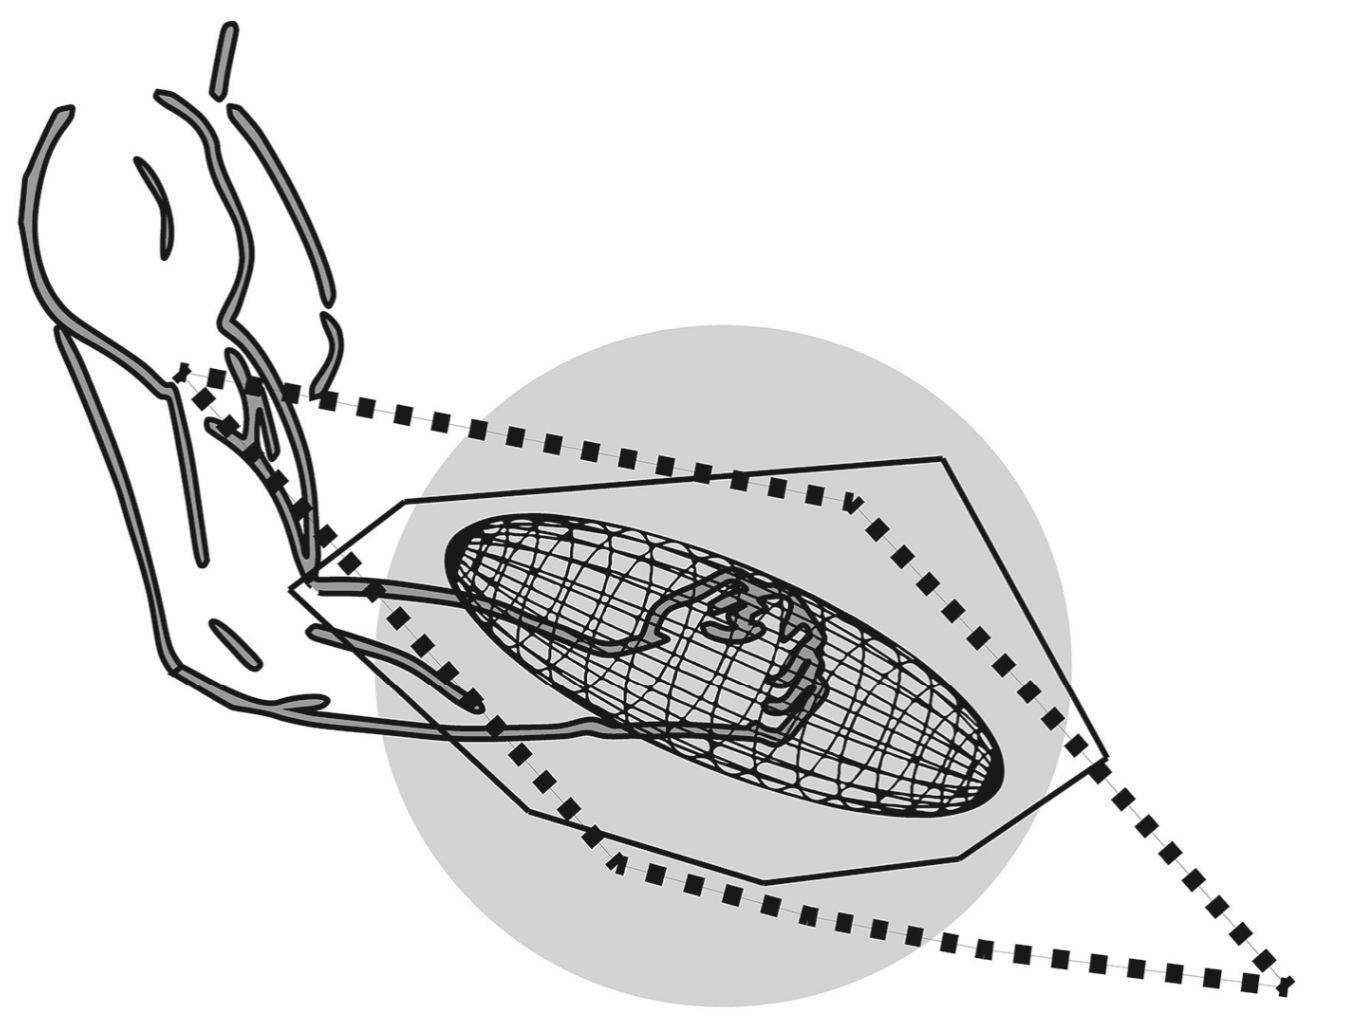
\includegraphics[trim={0 0 0 0},clip,width=0.4\linewidth]{img/chapter_1/rezzoug_2021.png}
    \caption{Representations of the simulated scaled force ellipsoid (wire-frame) and scaled force polytope (black squares) with measured force feasible set described in the sagittal plane in (\cite{rezzougUpperLimbIsometricForce2021b}).}
    \label{fig:rezzoug2021}
\end{figure}

This study also suggests the importance of considering a higher number of muscles than degrees of freedom to achieve a more physiologically accurate model of the upper limb.

To address this, in (\cite{hernandezIsometricForceCapabilities2015}) a scaled musculoskeletal model with 29 muscles and 7 degrees of freedom was used (adapted from the upper-limb model from (\cite{holzbaurModelUpperExtremity2005})) for 9 subjects. Similar to (\cite{rezzougUpperLimbIsometricForce2021b}), they used 26 force directions at the hand to gather experimental MVICs, and the convex hull of these measurements formed the measured force feasible set. For the \emph{in silico} analysis, they used a force polytope representation and incorporated muscle activations. They determined whether each muscle should be fully activated or not based on the direction of the exerted force. For a given posture and force direction $\mathbf{v}\in\IR^3$, they computed the moment arm matrix $-L^T \in \IR^{7\times 29}$. Each column of this matrix corresponds to the moment vector of a muscle. For each muscle, they orthogonally projected its moment vector onto $\im{J^T}$ and compared the angle between this projection and $J^T\mathbf{v}$. They assumed that a muscle contributes to a force direction $\mathbf{v}$ if its moment vector is aligned with $J^T\mathbf{v}$. This alignment is determined by the angle between the two vectors. If this angle is less than 90°, the corresponding muscle is fully activated (activation = 1); otherwise, it is not activated (activation = 0). They considered a large number of force directions $\mathbf{v}\in V$, with spherical coordinates $(\theta, \phi)$ where $\theta \in [0, 360$°$]$ and $\phi\in[0,180$°$]$ in 1° increments. This allowed them to characterize each muscle tension based on the considered force direction $\mathbf{v}$. Based on this muscle activation model, they defined the force polytope $\mathcal{MSFP}$ as follows:
\begin{align*}
    \mathcal{MSFP} = \left\{ \mathbf{f} \in\IR^3 \mid \mathbf{f} = (J^T)^+(-L^T\mathbf{t}(\mathbf{v}) - \mathbf{G}), \quad \mathbf{v}\in V \right\}
\end{align*}

Figure \ref{fig:hernandez2016} shows the difference between the computed force feasible set $\mathcal{MSFP}$ and the measured one for one subject in a specific posture.
\begin{figure}[!htb]
    \captionsetup{justification=centering}
        \centering
        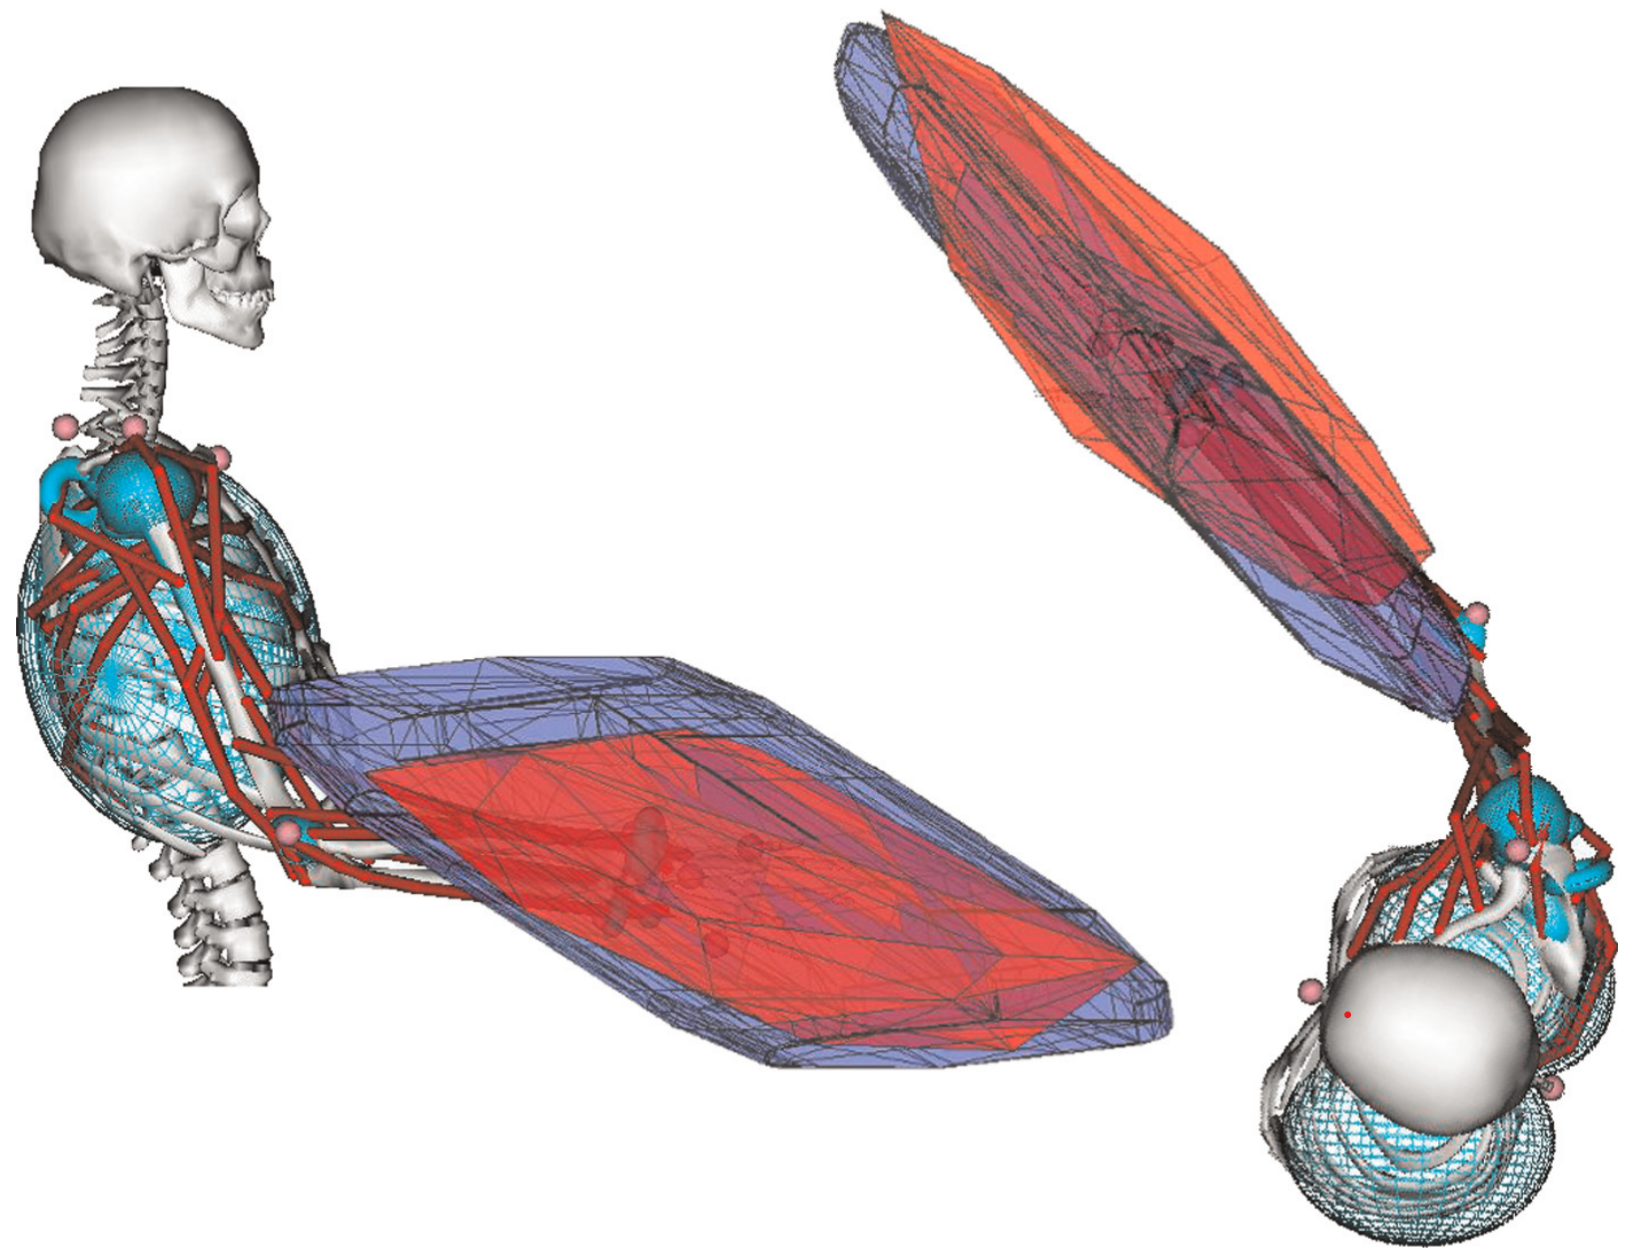
\includegraphics[trim={0 0 0 0},clip,width=0.7\linewidth]{img/chapter_1/hernandez_force.png}
    \caption{Measured (red) and computed (blue, $\mathcal{MSFP}$) force feasible sets for one subject in the sagittal plane, from (\cite{hernandezIsometricForceCapabilities2015}).}
    \label{fig:hernandez2016}
\end{figure}

Although the overall orientation of the computed force feasible set appears to be preserved, there are still significant differences in its proportions compared to the measured set. A key assumption in this experiment is that a muscle produces active tension only when it contributes to the force direction. This assumption leads to a polytopic shape of the resulting torque feasible set. The authors chose to orthogonally project (rather than intersect) the torque feasible set onto $\im{J^T}$. This choice of projection over intersection is important because it allows for a direct interpretation of the force direction with respect to the muscle joint torques. This is reflected in the authors' approach of considering specific muscle activations according to the force directions. If they had used the intersection operation instead of projection, this direct analogy between force direction and muscle activation would not be possible.

However, it is important to note that the overall orientation of the force polytopes computed by Hernandez et al. appears to be consistent with the experimental data. As shown by Hernandez et al., the angle between the principal axes of the computed and measured force feasible sets varied between 2.4° and 9.5° (in absolute value) across the subjects. This suggests that the orientation properties are largely determined by $(J^T)^+$, which is a key component of all the force feasible set formulations presented here. 

The presented studies have revealed several important properties of upper-limb force feasible sets and their representations. First, accurately modeling these sets may require considering a higher number of muscles than degrees of freedom. Second, muscle tension interactions appear to significantly influence the quality of the force feasible set, affecting its volume, elongation, and overall shape.

To further explore the shape of force feasible sets, we will now examine two studies that specifically focus on this aspect. The first study, (\cite{oshimaRoboticAnalysesOutput2000}), suggested that the set of isometric maximal forces produced at the hand in the transverse plane has a hexagonal shape. This hexagonal shape is a special case of a polytopic representation, where the forces are restricted to a 2D plane and two degrees of freedom are considered. Consequently, when the postures are not in singular joint configuration, the matrix $J^T$ is invertible, and the force feasible set becomes a linear transformation of the torque feasible set since $(J^T)^{-1}$ exists and is equal to $(J^T)^+$. However, the hexagonal shape, with its 8 edges, implies a specific constraint: only 4 muscles are present in the upper limb. The relationship between the edges of the torque feasible set and the number of muscles will be explored in more detail in Chapter \ref{chapter:2}. Although this assumption may not be physiologically accurate, it is worth noting that it could imply much simpler muscle representations for 2D force feasible sets. Similarly, (\cite{sasakiHigherDimensionalSpatial2010a}) conducted a similar experiment to (\cite{oshimaRoboticAnalysesOutput2000}), using different postures. They observed that `the feature of shape of the manipulating force polytope agrees with findings of Oshima et al. that the distribution of the hand force vector in a two-dimensional plane is a hexagonal shape', which further supports the hypothesis of a 4-muscle system.

Experimental results show that the produced hand forces can indeed be approximated by a hexagon, taking into account errors in the 8 force measurements (Figure \ref{fig:sasaki_hexagon}). This hexagonal shape was also observed in (\cite{oshimaRoboticAnalysesOutput2000}) but required a larger number of maximal force exertions to achieve it (Figure \ref{fig:oshima_force_hexagon}).
\begin{figure}[!htb]
    \captionsetup{justification=centering}
    \begin{minipage}{0.5\linewidth}
        \centering
        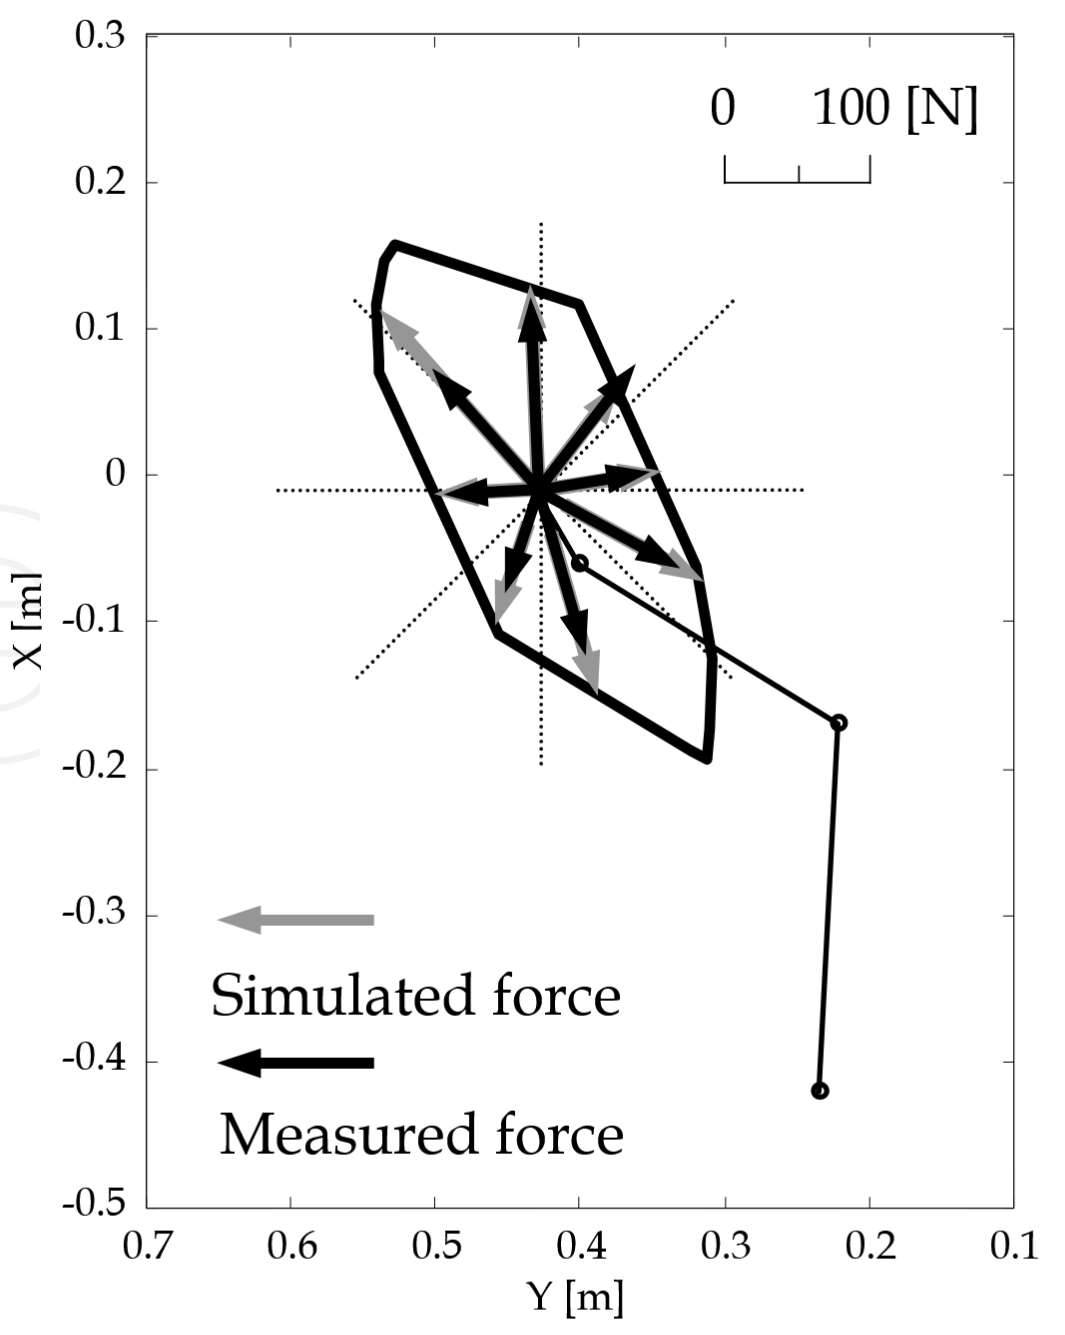
\includegraphics[trim={0 0 0 0},clip,width=0.8\linewidth]{img/chapter_1/sasaki_hexagon.png}
        \caption{Hexagon (black line) assumed in (\cite{sasakiHigherDimensionalSpatial2010a}) for 8 hand maximal force measurements (black arrows).}
        \label{fig:sasaki_hexagon}
    \end{minipage}
    \hfill
    \begin{minipage}{0.48\linewidth}
        \centering
        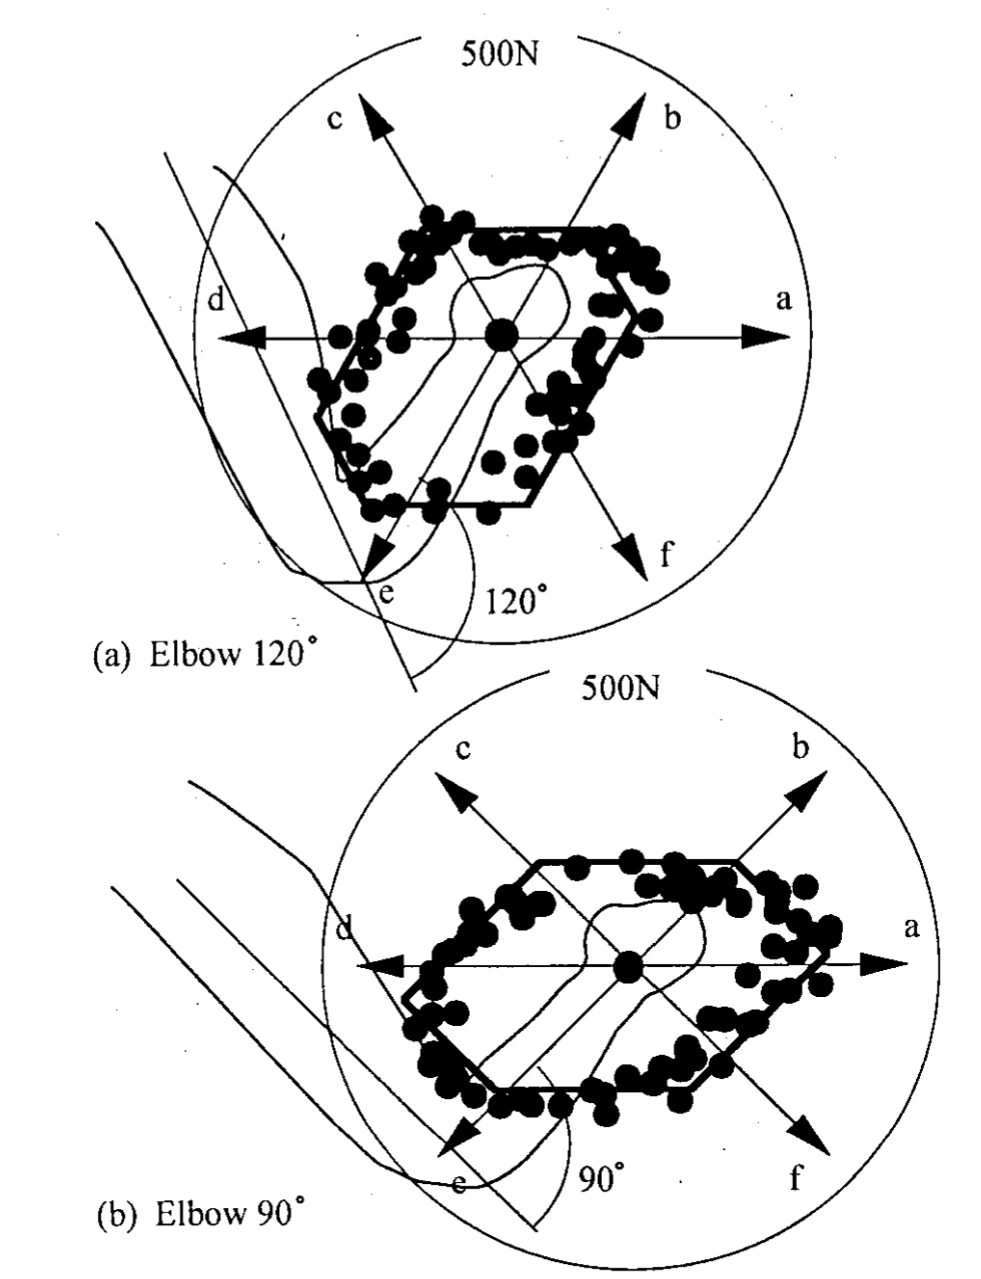
\includegraphics[trim={0 0 0 0},clip,width=0.8\linewidth]{img/chapter_1/oshima_force_output.png}
        \caption{(\cite{oshimaRoboticAnalysesOutput2000}):  maximal force measurements (black points) in two postures.}
        \label{fig:oshima_force_hexagon}
    \end{minipage}
\end{figure}

However, Oshima et al. acknowledged that an infinite number of hexagons could fit their data. Both experiments were based on prior assumptions about the number of muscles involved. It is also possible that other convex shapes with more edges, or even an ellipsoid, could have fit the experimental data equally well.


% ---------- SHOULD CORRECT ENGLISH FROM NOW
% ------------------------------------------
% ------------------------------------------
% ------------------------------------------

This subsection highlighted how inconsistencies appear between \emph{in silico} and \emph{in vivo} force feasible sets. Consequently, it is relevant to consider how accurately force feasible sets can be modeled to reflect an individual's muscles, especially given the uncertainty regarding which \emph{in silico} modeling choices best reflect \emph{in vivo} measurements \cite{sutjiptoComparisonStrengthProfile2024a}.

% This subsection highlighted how inconsistencies appear between \emph{in silico} and \emph{in vivo} force feasible sets. As such, it is relevant to consider to what extent force feasible sets can be modeled to reflect the muscles of an individual, as it is unclear which modeling choice of \emph{in silico} force feasible set may best reflect \emph{in vivo} experimental measurements (\cite{sutjiptoComparisonStrengthProfile2024a}). 

% The next subsection focuses on this challenge, and how this observed difficulty can be quantified in order to better direct the modeling of force feasible sets specifically to an individual.

% \subsection{Measuring the feasibility of musculoskeletal muscle personalization}
% \label{subsec:sensitivity_approaches}

% % \subsubsection*{La Delfa, potvin} \cite{ladelfaArmForceField2017}, \cite{ladelfaEquationsPredictFemale2014}, \cite{ladelfaPredictingManualArm2016a}


% In musculoskeletal modeling, \emph{muscle personalization} refers to the process of tailoring a generic muscle model to reflect the specific biomechanical characteristics of an individual. This involves adjusting the parameters defining the musculoskeletal model and match the individual's unique anatomy and physiology (\cite{fernandezNarrativeReviewPersonalized2023}). The newly constructed model, termed a \emph{personalized} model or a \emph{subject-specific} musculoskeletal model, is validated by comparison against experimental data, such as its capabilities to reproduce a specific movement or net joint force and moments.

% Requiring a personalized model depends on the research question, as recalled in (\cite{saxbyMachineLearningMethods2020}), where the authors argue that the use of a more \emph{generic} model is of interest when the objective is not particularly sensitive to model personalization. For instance, the study of change of muscle function after a surgical relocation of muscle attachment points does not require a personalization process (\cite{akhundovSubjectspecificMusculoskeletalModelling2022}). In the contrary, subject-specific models should be favored on a case-by-case basis, as for instance when a generic model can not properly represent \emph{in vivo} lower limb net joint moments produced by muscles in a simulated sprint and cut task (\cite{akhundovSubjectspecificMusculoskeletalModelling2022}).

% \emph{In silico} force feasible sets contain, through their set-theoretic nature, information of a posture, muscle geometry and force-generating characteristics, but also how muscles are dependent of each other activations. All of these parameters are included in their mathematical definition. As it is possible to scale a generic model to fit an individual, it can be assumed that a given upper-limb posture is known, and also the bone geometry of an individual. As such, quantifying how muscle parameters (maximal isometric force, optimal fiber length, tendon slack length, geometrical path, etc.) influences force feasible sets is a necessary step to evaluate to what extent a personalization process might be feasible. Such influence can be quantified through a \emph{sensitivity analysis}

% Evaluating the \emph{sensitivity} of a function $f\,\colon X \to Y$ consists on measuring how the \emph{topology} of $X$ affects the topology of $Y$ under $f$. The topology of a mathematical structure refers to the general notions of continuity, limits, connectedness, shape, smoothness, etc. Small changes in $X$, like tweaking a parameter, might lead to significant shifts in the topology of $Y$, indicating high sensitivity. This means the output is heavily influenced by that particular parameter. Conversely, if large changes in $X$ barely affect $Y$'s topology, the output is insensitive to those inputs. Sensitivity analysis thus comprises of methods to obtain quantitative insights on a given mapping, in order to ``draw out the maximum capabilities of mathematical modeling'' (\cite{rabitzGeneralFoundationsHighdimensional1999}). 

% % While it is natural to consider that $f$ shapes $Y$ according to $X$, a more rich (mathematically speaking\footnote{This is also referred as the \emph{fiber} theory, or the study of pre-images.}) approach consists of seeing how the variability of $X$ is according to the variability of $Y$. In other word, this approach studies the variability of $X$ as $X = f^{-1}(Y)$ where $f^{-1}$ is the pre-image mapping, which corresponds to the usual inverse of $f$ if $f$ is bijective. The first approach is termed a \emph{local} sensitivity analysis, while the second is a \emph{global} analysis (\cite{borgonovoSensitivityAnalysisReview2016}).

% There are two types of sensitivity analyses, termed \emph{local} and \emph{global} methods (\cite{borgonovoSensitivityAnalysisReview2016}). Local methods perform an analysis in a relatively small (sometimes infinitely small) neighborhood around a chosen element of the domain $X$. This includes for instance to compute the partial differentials of a function $f$, if it is differentiable, and study the properties of its Jacobian matrix (first order differentials) and Hessian matrix (second order differentials). Other methods would involve finite differences, if $f$ is not necessarily differentiable, and \emph{screening} methods (\cite{paleariSensitivityAnalysisUsing2021}) which are more adequate when evaluating $f$ is time-consuming and/or ressource-heavy. Essentially, screening methods evaluate $f$ on a limited number of other elements around a chosen element of $X$. In our context, this would require for instance to consider a fixed parameterization of a musculoskeletal model, and create small perturbations around it to gauge how a perturbated parameter would influence the produced force feasible sets.

% On the other hand, global (or probabilistic) sensitivity methods assign a probabilitic model to describe the variability of the domain $X$ in regard to values of $Y$. These are particularly adequate methods for a general understanding of $X$ under $f$, notably it can tell us if $X$ is strongly irregular with a lot of local minima or if it a surface which consists of wide local minima largely spaced in between them. 

% With these considerations, common sensitivity analyses may not be adapted, as they usually consider a vector-to-vector and not a set-to-set relationship. As such, we focuses on the challenges induced by the set-theoretic nature of force feasible sets for sensitivity analyses. 

% Therefore, this section serves as introducing methodologies to evaluate how muscle parameters influence force feasible sets, in order to determined to what extent a musculoskeletal model personalization process may induce difficulties using force feasible sets. In this regard, Chapter \ref{chapter:4} will thus provide an adapted sensitivity analysis, based on a personalization process, which will lead to better characterization of these challenges.

% % First hints have been experimentally shown that these sets proportions vary according to an individual. For instance in (\cite{hernandezIsometricForceCapabilities2015}), the authors measured maximal isometric forces in various directions for nine participants, and the resulting measured force feasible sets were shown to be different in shape, and global size, compared to \emph{in silico} force feasible sets. 

% % When referring to a personalized model in this chapter, we shall strictly consider the personalization of a \emph{musculoskeletal model} and its parameters describing muscle force models and produced torques. For instance, the following study implies, in a sense, the personalization of a model which is a curve: \cite{aldiniRealtimeEstimationStrength2021} propose a 4 dimensional curve to modelize the \emph{strength capacity} of the hand. Their goal was to create a parametric equation (with respect to the pose of the upper limb) to model the strength capacity at the hand of an individual in a context of physical Human-Robot collaboration of an operator's hand and a robot end-effector. They assumed the feasible tension set to by an orthotope. The strength fitting was made offline on 910 hand positions. The direction of the force for each pose is fixed for each pose, and defined to be along the direction from the hand to the thorax centre. DOFs at the wrist were ignored. The resulting curve, for each of the 6 participants, seemed to predict the variations in amplitude of the measured forces, and this approach presents an average RMSE for all 6 participants of $37.67\pm 8.02$ N between the created curves and experimental measurements in 13 different postures. As the authors mentionned, this could be due to loss of accuracy in the positions. This method is thus a parametric personalization of a musculoskeletal model in order to study exerted maximal forces in specific directions depending on the individual posture.

% % While relevant in practice, this type of personalization do not allows to consider other force directions at the same time.



% % In (\cite{delpInteractiveGraphicsbasedModel1990a}), it was studied how, in the lower limb, the muscle path (represented as a series of line segments) as well as the musculotendon parameters (maximal isometric force, optimal fiber length and tendon slack length) influence the generation of each muscle joint force and moment. For this sensitivity analysis, the authors considered that a muscle to span a 1-degree of freedom revolute joint, and they perturbated the tendon slack length, the optimal fiber length, as well as the joint angle at which the maximal isometric muscle force is produced for a given muscle. They found that depending on the ratio tendon slack length/muscle moment arm, the ge TO REDO

% In (\cite{carmichaelUpperLimbStrength2015}), the authors studied \emph{in silico} how muscle parameters such as the maximum isometric force, optimal fiber length and tendon slack length influence the exertion of a maximal force at the hand in 14 different directions, for 46 hand locations while keeping the trunk fixed. They considered Holzbaur's upper limb model (\cite{holzbaurModelUpperExtremity2005}) and locked the wrist and finger joints, leaving 3 degrees-of-freedom in the shoulder and 1 in the elbow. They effected a local sensitivity analysis so that they perturbated one muscle parameter by perturbating it by $\pm 1\%$ from its original parameter's value to consider an approximation of the partial derivative function returning the maximal exerted force magnitude. For each direction and posture, they evaluated the sensitivity index $\varepsilon_{p_M}$ of the muscle parameter $p_M$ of muscle $M$ as:
% \begin{align*}
%     \varepsilon_{p_M} = \left| \frac{(S_{p_M}^+ - S_{p_M}^-) / S_{p_M}^0}{(p_M^+ - p_M^-)/p_M^0} \right|
% \end{align*}
% where $S_{p_M}^0$ is the maximal exerted force magnitude computed with no variation of the initial parameter value $p_M^0$, $S_{p_M}^+$ is the magnitude computed with a $1\%$ variation of the initial parameter value ($p_M^+$) and $S_{p_M}^-$ is the magnitude computed with a $-1\%$ variation of the initial parameter value ($p_M^-$). 

% The authors concluded this experiment by comparing the sensitivity of parameter types for all muscles, so that the tendon slack length and the optimal fiber length seem to be the most sensitive, then followed by the maximal isometric force of muscles and the pennation angle. They also conducted the same experiment with perturbations of $\pm 5\%$, which led to the same conclusion. This study goes much further and focus on how much more sensitive are the parameters in pathological cases, but we focus on the methodology more than the conclusions. 

% A similar method based on slightly perturbating muscle parameters can be found in (\cite{delpInteractiveGraphicsbasedModel1990a}) to characterize how muscle geometric and force-generating parameters affect maximal produced joint torques. 

% Also, (\cite{flores-hernandezScapulothoracicRhythmAffects2019}) studied the sensitivity of the shoulder motion for glenohumeral joint forces to show that it does have an impact. 

% Lindbeck et al., 2023 \cite{lindbeckPredictionsThumbHand2023}

% These experiments perturbated one parameter at a time. When considering exert.

% Global sensitivity analyses seem to be more rare in the literature, as they necessarily involve more computational ressources. Nevertheless, a study from 2006 by Langenderfer et al. cite{langenderferProbabilisticModelGlenohumeral2006} considered multivariate Gamma distributions to probabilistically simulate the effects of variability in PCSAs, moment arms and the muscle length-tension relationships for muscle accross the shoulder. They considered tendons to be rigid. In other words, their method consist on modeling the intra-variability of characteristics of multiple shoulder muscles in cadaveric specimens by Gamma distributions, and correlate them with the intra-variability of experimentally measured force and joint torques over the glenohumeral external rotation of 120 healthy subjects, in a specific posture. The posture considered the elbow to be flexed at $90$°. Subjects  were asked to perform voluntary maximal isometric effort around the shoulder external rotation axis.

% They evaluated the sensitivity of these parameters towards the developped muscle forces and joint torque over the glenohumeral external rotation. Tendons were modeled as rigid. Experimental glenohumeral strength force and moment were gathered for 120 healthy individuals (60 males, 60 females) in a upper limb posture with 90° elbow angle, performing maximal effort around the shoulder external rotation axis. Also, the authors gathered characteristics of 3 shoulder muscles (supraspinatus, infraspinatus and teres minor). They gathered each muscle moment arms in the reference posture for 10 glenohumeral cadaver specimens. They also gathered the optimal fiber length, the physiological cross-sectional area and tendon slack length of each muscles in order to form a force-length relationship.

% perturbations of muscle parameters (PCSA, moment and muscle length tension relationship), look at produced muscle forces and joint torque.

% % \subsection{Personalization of muscle parameters and measurements}
% % \label{subsec:sensitivity_ffs}

% % Measurements:
% % Strength profile: \cite{sutjiptoComparisonStrengthProfile2024}
% % In the horizontal plane: \cite{jannijhofMaximumIsometricArm2006}

% % \subsubsection*{Personalization examples with exerted forces}

% % In 2000, Oshima et al. \cite{oshimaRoboticAnalysesOutput2000} considered the force feasible set (as a polytope) of a planar serial kinematic chain with 2 revolute joints to represent the upper limb shoulder and the elbow, as well as 6 muscles crossing either one joint or two. The authors wanted to identified each muscle exerted force from the produce force polytope shape. However, the fact only planar forces and 2 joints are considered means that the force polytope has the particular shape of a \emph{zonotope}. Indeed, they considered postures where the jacobian transpose matrix is invertible, so that the force feasible set is a linear transformation of the torque feasible set, represented in their case a zonotope (projection of the muscle feasible tensions hyperrectangle). Due to this specific case, they succeeded, in silico and in vivo on a single participant, through geometric reasonning on the symmetries of the edges on the zonotope surface, which are directly related to th muscle (more details will be provided in chapter \ref{chapter:2}). Also, the authors claimed that the force feasible sets produced by the individual has a zonotopic shape, where the given representations of measured forces in this article could also allow us to consider an ellipsoid representation of these measures. They acknowledge this arbitrary choice of an hexagone (a type of 2D zonotope) but stating that there could have been an infinite amount of hexagons to fit the data.
% % \begin{figure}[!htb]
% %     \captionsetup{justification=centering}
% %         \centering
% %         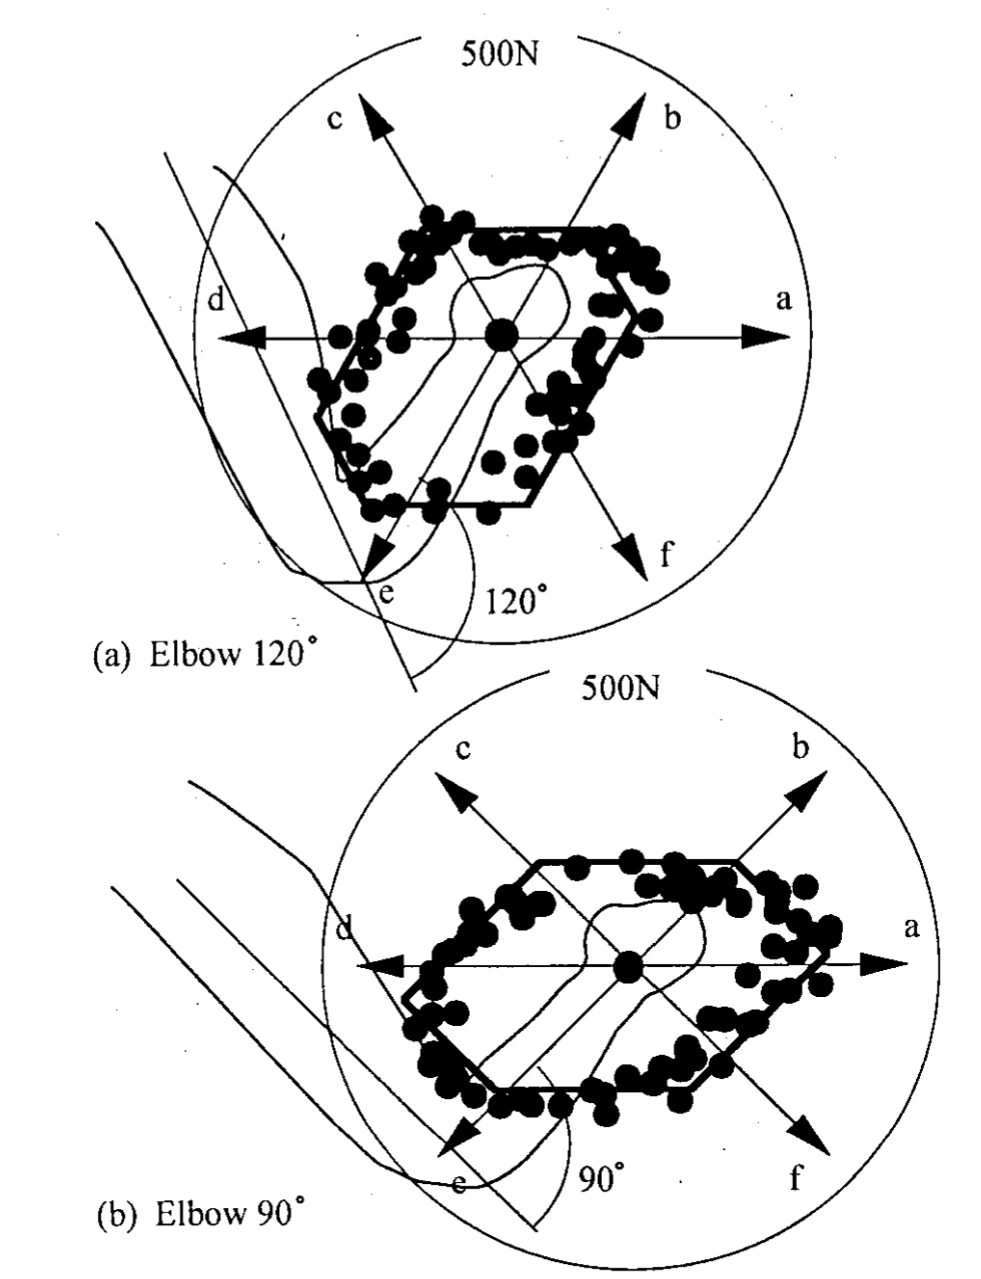
\includegraphics[trim={0 0 0 0},clip,width=0.4\linewidth]{img/chapter_1/oshima_force_output.png}
% %     \caption{Oshima et al. \cite{oshimaRoboticAnalysesOutput2000} maximal force measurements (black points) in two postures.}
% %     \label{fig:oshima_force_output}
% % \end{figure}


\subsection{Conclusion}
This subsection focused on the process of measuring maximal isometric forces at the hand in a specific posture, from the challenges of obtaining accurate maximal voluntary isometric contractions (MVICs) to the construction of \emph{measured} force feasible sets. 

The challenges associated with measuring MVICs may explain the scarcity of data on MVICs measured in different directions for a single posture. In this regard, Chapter \ref{chapter:5} details an experimental protocol for collecting MVICs in 26 different directions for 4 distinct postures in 10 subjects. 

Furthermore, there is no standardized procedure for determining the number and directions of measured forces required to adequately represent a force feasible set. Therefore, Chapter \ref{chapter:2} draws theoretical conclusions about the natural shape of a force feasible set when a large number of muscles are considered. This chapter will demonstrate that an ellipsoidal shape is sufficient to represent force feasible sets. From an experimental perspective, this reduces the number of maximal forces that need to be measured, as a 3D ellipsoid can be described by only 9 points on its surface, and a 2D ellipse by only 5. 

Finally, although there is no consensus on which force feasible set description best reflects the characteristics of maximal isometric forces, this thesis proposes a simpler theoretical representation (Chapter \ref{chapter:3}). This representation is then adapted and compared with experimental data (Chapter \ref{chapter:5}) to evaluate its relevance. Since the extent to which force feasible sets encapsulate information about muscle geometry and muscle tensions remains unclear, the next section investigates how these sets are influenced by muscle architecture and force-generating properties. 

\section{General conclusion}
This chapter encompassed a review of the literature concerned with the required biomechanical tools for a complete study of maximal isometric forces in a set-theoretic framework. First, we focused on how to model them \emph{in silico}, via force feasible sets, and showed how computational difficulties arise, necessitating the development of better computational algorithms. Second, we examined how experimental measurement of maximal isometric forces is not necessarily coherent with \emph{in silico} force feasible set models, necessitating improved modeling of force feasible sets and more judicious selection of measurement directions to mitigate experimental challenges. Finally, the chapter explored sensitivity techniques used in biomechanics, as these methods could give insights on how muscle tensions and their interactions are reflected in the set-theoretic approach of force feasible sets. The following paragraphs summarize for each section the difficulties encountered in the literature and how this thesis addresses them.

In Section \ref{sec:muscu_model_in_silico_ffs}, the dynamics of the human upper-limb were represented \emph{in silico} using a serial kinematic chain. This allowed for the description of forces applied to the upper-limb, and the \emph{force feasible set} formulation was given in a very general case as well as in isometric conditions with a fixed upper-limb posture. The construction of the force feasible set is inherently geometric: it involves the \emph{projection} of a higher-dimensional set, termed the \emph{muscle tension feasible set}, onto the torque space, which is then \emph{intersected} by a vector subspace of dimension 3. Different models, based on geometric assumptions about the muscle tension feasible set, are used to describe the force feasible set: if each muscle acts independently of other muscles, the resulting force feasible set is a 3D \emph{force polytope}. When muscle tensions are interdependent, the resulting shape is more rounded, as with \emph{force ellipsoids} (assuming an ellipsoidal tension feasible set). These representations are used in different contexts, depending on whether muscle independence is assumed (polytope) or inter-muscle dependencies are considered (typically modeled using ellipsoids). A force polytope representation is challenging to visualize, as it involves combinatorial processes to express its surface, whereas force ellipsoids are much simpler. This combinatorial increase in time complexity necessitated strategies for reducing computation time, which are explored in Chapter \ref{chapter:2}. This chapter presents a new vertex enumeration technique to describe the torque feasible set surface.

Section \ref{sec:modeling_muscle_tensions} delved into the experimental process involved in collecting maximal isometric forces, from the standardized protocol of maximal voluntary isometric contractions (MVICs), to the creation of force feasible sets from these measurements within a fixed posture. Inconsistencies in the proportions and shapes were observed between \emph{in silico} force feasible sets and experimental measurements. Since these characteristics depend on how the upper-limb is modeled \emph{in silico} (\emph{e.g.}, number of muscles, level of detail in muscle geometrical paths), Chapter \ref{chapter:3} of this thesis offers a new geometrico-probabilistic perspective on how these \emph{in silico} force feasible set characteristics behave as the theoretic complexity of a musculoskeletal model increases. As such, a unified representation of force feasible sets as ellipsoids will be computable under specific theoretical assumptions (namely, a \emph{high} number of muscles). Furthermore, Chapter \ref{chapter:4} will assess whether the biomechanically validated musculoskeletal model of the upper-limb from (\cite{holzbaurModelUpperExtremity2005}) has sufficient muscle detail to apply these assumptions in the context of muscle personalization. This section also highlighted a lack of experimental data concerning multiple maximal isometric force exertions in a fixed posture; Chapter \ref{chapter:5} addresses this by providing new experimental measurements of maximal isometric force exertions in 4 different postures for 10 participants.

% Section \ref{sec:feasibility_personalization} focused on the challenges of retrieving muscle parameters from a collection of maximal isometric forces, given the set-theoretic nature of this data. Sensitivity analysis methods used in biomechanical contexts were compared to determine the most relevant approach for considering the geometric construction of force feasible sets. Based on this comparison, Chapter \ref{chapter:4} introduces a new adapted sensitivity analysis methodology, which provides insights into the challenges of musculoskeletal model muscle personalization from force feasible sets, and demonstrates that muscle geometry parameters are not the most influential factors determining the difficulties occuring in a personalization process.


\chapter{New efficient edge-based zonotope vertex enumeration}
\label{chapter:2}
\usection{Introduction}
To understand how \emph{in silico} isometric force feasible sets encompass both muscle tension interactions and muscle biomechanical characteristics, notably their paths along bones and their exertable tensions, this thesis delves into the geometric process of exerting maximal isometric forces. A force feasible set $\mathcal{F}$ is described by two successive geometric set-theoretic operations: 1) the projection of a tension feasible set $\mathcal{T}$ onto the joint torque space, creating the \emph{torque feasible set}, and 2) the intersection of the torque feasible set with a vector space. 

A main objective of this thesis is to understand the set-theoretic properties of force feasible sets to guide the personalization of muscle parameters in musculoskeletal models, which is addressed in Chapters \ref{chapter:4} and \ref{chapter:5}. As a first step toward this understanding, this chapter studies specifically the projection of the tension feasible sets — more precisely, it examines how the torque feasible set encompasses muscle properties. 

To assess how tension interactions are projected onto the torque space, different models of these interactions must be considered. Chapter \ref{chapter:1} explained that varying the model of the tension feasible set leads to distinct force feasible set characterizations, such as force polytopes and force ellipsoids. This chapter and Chapter \ref{chapter:3} are strongly linked, as they focus on tension feasible set modeling and its impact on the resulting geometric construction. While this chapter concentrates on polytopic representations, Chapter \ref{chapter:3} will study more rounded shapes. Both chapters require different mathematical frameworks to better account for tension feasible set modeling; hence, they are presented separately. 

With $\mathcal{T}$ modeled as an orthotope (a hyperrectangle), this chapter approaches the understanding of the projection process through a combinatorial lens. This approach, which encompasses mathematical results related to \emph{counting} objects, is particularly well-suited for polytope-related studies, as polytopes possess inherent combinatorial properties that reflect their shape and volume (\cite{grunbaumConvexPolytopes2013}). However, such properties can be challenging to discern, as they may not have an explicit form or simple interpretation. Dedicated algorithms can provide a different perspective on these results by iteratively examining combinatorial solutions to a problem and selecting specific ones. This selection process is inherently informative (\cite{barvinokComputingEhrhartQuasipolynomial2005}; \cite{lopezPolytopeIntersectionHalfspaces2024a}).

Therefore, this chapter presents an algorithm that computes the vertices delimiting the projection of a tension feasible set, modeled as a hyperrectangle, onto the torque space. The resulting shape is termed a \emph{zonotope} and is a specific type of polytope exhibiting central symmetry. Because these vertices are \emph{unique} to a zonotope, their enumeration reflects how the bounds of muscle tensions are projected onto the torque set. The following paragraphs focus on clearly introducing this concept in the context of \emph{in silico} force feasible sets.

In this thesis, $\mathcal{T}\subset \IR^m$ denotes the set of all exertable tensions by $m$ muscles, also termed the tension feasible set. The force feasible set $\mathcal{F}\subset \mathbb{R}^3$ at the end effector of an $n$ degrees-of-freedom kinematic chain in a given posture is expressed as:
\begin{align*}
    \mathcal{F} = \left\{\mathbf{f}\in\IR^3\mid \exists \mathbf{t}\in \mathcal{T},\quad J^T\mathbf{f} = -L^T\mathbf{t} - \mathbf{G}\right\}
\end{align*}
where $J^T\in \mathbb{R}^{n\times 3}$ is the projection of the end-effector Cartesian forces onto the torque space, $L^T\in \IRnm$ is the projection of muscle tensions onto the torque space, and $\mathbf{G}\in\IRn$ is the gravity torque vector.
As we will focus in this chapter on only the projection of $\mathcal{T}$ onto the torque space, we define the \emph{torque feasible set} as the following:
\begin{align*}
    \left\{\tau \in \IR^n \mid \exists \mathbf{t}\in\mathcal{T}, \quad \tau = -L^T\mathbf{t} - \mathbf{G}\right\}
\end{align*}

$\mathcal{T}$ is assumed to be shaped as a $m$-orthotope (a hyperrectangle in $m$ dimensions) (Fig. \ref{fig:tension_set_orthotope}). This shape models how muscles can act together: it allows all muscles to exert their maximal tension simultaneously, which will be necessarily reflected onto the torque space (Fig. \ref{fig:joint_torque_simple_2D}). More precisely, for each exertable tension $t_i$ of a muscle $m_i$, there exist positive lower and upper bounds, denoted $\underline{t_i}$ and $\overline{t_i}$, defining the feasible tensions exertable by muscle $m_i$. The upper bound corresponds to the feasible muscle tension when the muscle is fully activated, while the lower bound relates to its passive tension when it is not activated.
\begin{figure}[!htb]
%   \captionsetup{justification=centering}
  \begin{minipage}{0.39\linewidth}
    \centering
    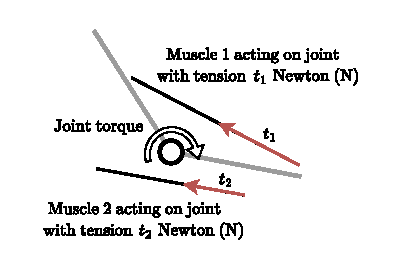
\includegraphics[trim={20 0 20 0}, clip, width=1\linewidth]{img/chapter_2/joint_torque_simple_2D.pdf}
    \caption{Simplified arm with one degree-of-freedom equipped with two muscles described as segments.}
    \label{fig:joint_torque_simple_2D}
  \end{minipage}
  \hfill
  \begin{minipage}{0.59\linewidth}
    \centering
    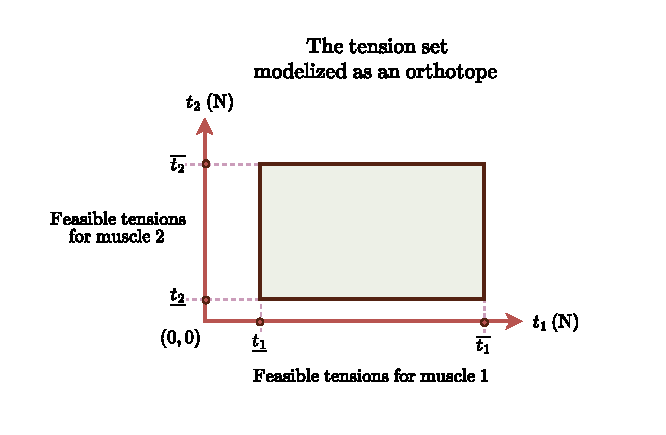
\includegraphics[trim={25 20 40 16}, clip, width=0.92\linewidth]{img/chapter_2/tension_set_orthotope.pdf}
    \caption{A muscle exerts tension in a feasible range of values. The set of all tension combinations $\mathcal{T}$ is shaped as an orthotope.}
    \label{fig:tension_set_orthotope}
  \end{minipage}
\end{figure}

While the assumption of independent exertion of tensions is plausible for a cable robot, human muscle activations are subject to neuromotor control, the laws of which are not yet fully understood. In cable robotics, if the feasible tensions of the cables (modeled as line segments) are assumed to be independent, the tension feasible set $\mathcal{T}$ takes the shape of an orthotope.

Geometrically, the torque feasible set is thus a \emph{zonotope}, \emph{i.e.}, a specific type of polytope described as a projection of a higher-dimensional cube. To compute the vertices of a zonotope, note that an $m$-orthotope is the image of an $m$-cube under an invertible affine transformation. Without loss of generality, $\mathcal{T}$ can be equated to the $m$-dimensional cube $[0,1]^m$, as shown in Figure \ref{fig:invertible_transfo_cube_orthotope}. An $m$-orthotope and an $m$-cube are said to be \emph{affinely equivalent}. 
\begin{figure}[!htb]
  \captionsetup{justification=centering}
  \begin{minipage}{1\linewidth}
    \centering
    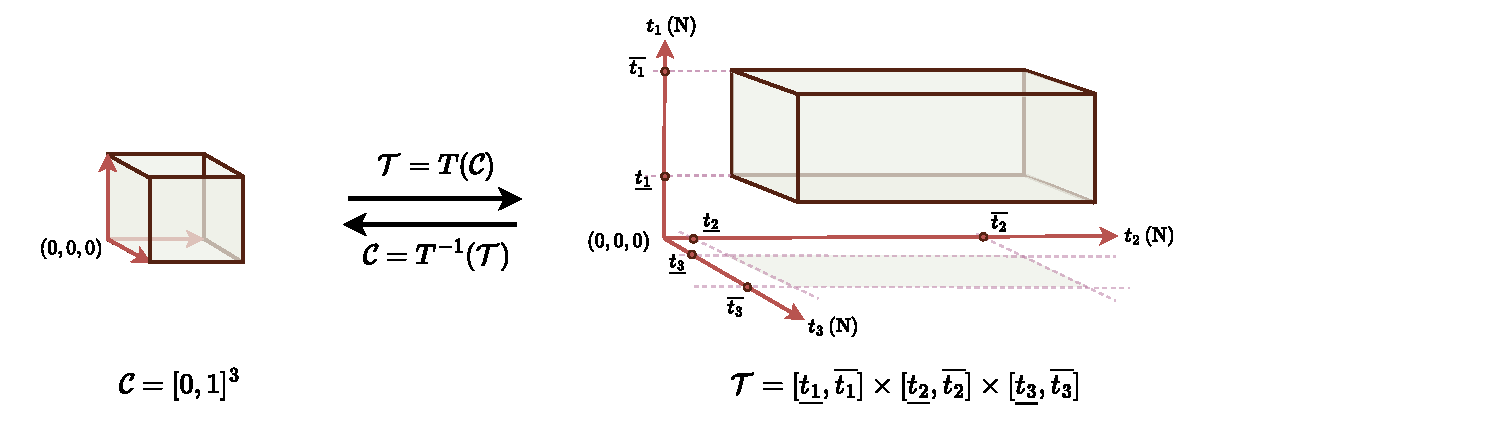
\includegraphics[trim={20 20 150 0}, clip, width=1\linewidth]{img/chapter_2/invertible_transformation.pdf}
    \caption[]{To consider the torque feasible set as a projection of the unit cube $\mathcal{C}=[0,1]^3$, consider the invertible affine transformation $T\,\colon \IR^3 \to \IR^3$ defined as:
    \begin{minipage}{\linewidth}
      \begin{align*}
        T(\mathbf{t}) &= D\mathbf{t} + \underline{\mathbf{t}}, \quad \text{for } D = \begin{pmatrix}
          \overline{t_1} - \underline{t_1} & 0 & 0 \\
          0 & \overline{t_2} - \underline{t_2} & 0 \\
          0 & 0 & \overline{t_3} - \underline{t_3}
        \end{pmatrix} \text{ and } \underline{\mathbf{t}} = \begin{pmatrix}
          \underline{t_1} \\ \underline{t_2} \\ \underline{t_3}
        \end{pmatrix}
      \end{align*}
    \end{minipage}

    Thus, $\mathcal{T} = T(\mathcal{C})$ and the torque feasible set is described as 
    $\left\{\tau \in \IR^3 \mid -LD\mathbf{t} -L\underline{\mathbf{t}} - \mathbf{G},\quad \mathbf{t}\in\mathcal{C}\right\}$, which is clearly an affine projection of a cube, so it is a zonotope by definition.}
    \label{fig:invertible_transfo_cube_orthotope}
  \end{minipage}
\end{figure}

Zonotopes have multiple possible representations, including a non-squared matrix, a set of vertices, delimiting hyperplanes, or even \emph{cells}, which characterize the cube vertices whose projections are the zonotope vertices. Several algorithms exist to transition from one representation to another, the goal of which is to be efficient in time and space. This chapter offers a new perspective on representing zonotopes using their edges and describes an algorithm to compute them directly from a matrix representation of a zonotope. To achieve this goal, let's first delve into zonotope formalism.

For two sets of vectors $A$ and $B$ in $\IR^n$, their \emph{Minkowski sum}, denoted $A\bigoplus B$, is defined as $A\bigoplus B = \left\{ a+b\in \IR^n \mid a\in A,\, b\in B\right\}$. 
Let $\Zono \subset \IRn$ be an $n$-zonotope, \emph{i.e.}, 
the Minkowski sum of $n$-dimensional segment vectors $\Zono = \mathbf{c} + \bigoplus_{i=1}^m \alpha_i \mathbf{g}_i$, where $\mathbf{c} \in \IRn$, $\mathbf{g}_i \in \IRn$ for $i=1,\dots,m$ such that all the $\mathbf{g}_i$ span $\IRn$, and $\alpha_i\in[0,1]$. This corresponds to the following set:
\begin{align*}
  \Zono &= \left\{ \mathbf{z} \in \IR^n \mid \mathbf{z} = \mathbf{c} + \sum_{i=1}^m \alpha_i \mathbf{g}_i,\quad \alpha_i \in [0,1],\, \mathbf{c}, \mathbf{g}_1,\cdots,\mathbf{g}_m\in\IR^n \right\}
\end{align*}

The vectors $\mathbf{g}_i$ are called \emph{generators} and are usually concatenated into the columns of a matrix $G\in\IRnm$. For conciseness, a zonotope is denoted directly using its translation and its generators as $\Zono(\mathbf{c}, G)$, or $\Zono(G)$ if there is no translation. The notation $\Zono(n, m)$ is also convenient to directly refer to the size of the matrix $G$. The generators are assumed to be non-null, and any combination of $n$ of them is assumed to span $\IRn$. In this case, the generators are said to be in \emph{general position}.

\begin{figure}[!htb]
  \captionsetup{justification=centering}
  \begin{minipage}{0.49\linewidth}
    \centering
    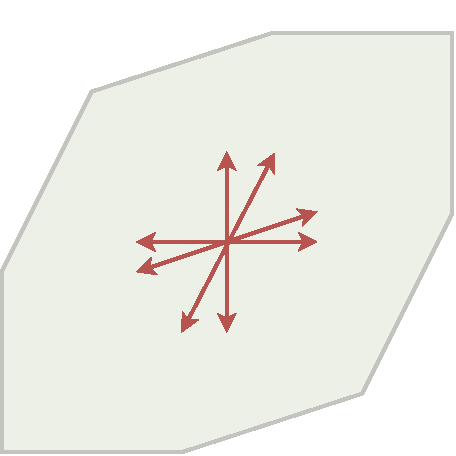
\includegraphics[trim={0 0 0 0},clip, width=0.6\linewidth]{img/chapter_2/zonotope_2d_4g.pdf}
  \end{minipage}
  \hfill
  \begin{minipage}{0.49\linewidth}
    \centering
    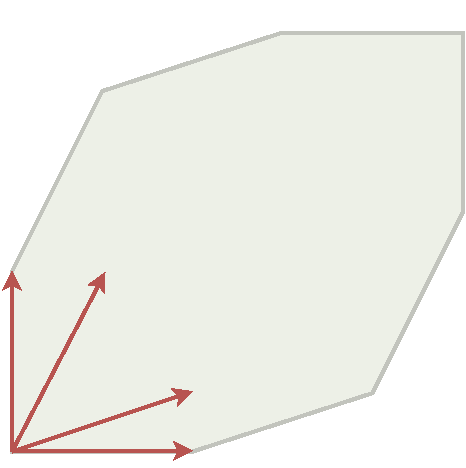
\includegraphics[trim={0 0 0 0},clip,width=0.6\linewidth]{img/chapter_2/zonotope_2d_4g_alt.pdf}
  \end{minipage}
  \caption{Both constructions lead to the same 2D zonotope generated by $4$ generators: the differences lie in the bounds defined for $\alpha_i$, which are $[-1,1]$ for the left zonotope and $[0, 1]$ for the right, and the center $\mathbf{c}$.}
  \label{fig:a_simple_zonotope}
\end{figure}

A zonotope is a specific type of convex polytope; therefore, it can be described via its vertices ($\mathcal{V}$-representation) or a set of inequalities ($\mathcal{H}$-representation), as shown in Figure \ref{fig:zonotope_vertices_hyperplanes}. Several zonotope applications include their use as bounding volumes in collision detection (\cite{guibasZonotopesBoundingVolumes}), as bounds for disturbances and measurement errors (\cite{scottInputDesignGuaranteed2014}), and in approximating the domain of a function of several variables (\cite{stinsonRandomizedAlgorithmEnumerating2016}). More recently in robotics, a neural network was used to predict a path of reachable sets in an environment crowded with dynamic obstacles modeled as zonotopes (\cite{shamsahSociallyAcceptableBipedal2024}).

\begin{figure}[!htb]
  \captionsetup{justification=centering}
  \begin{minipage}{0.49\linewidth}
    \centering
    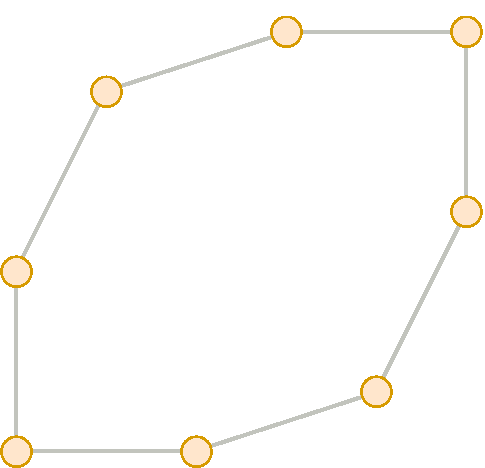
\includegraphics[trim={0 0 0 0},clip, width=0.6\linewidth]{img/chapter_2/zonotope_vertices.pdf}
  \end{minipage}
  \hfill
  \begin{minipage}{0.49\linewidth}
    \centering
    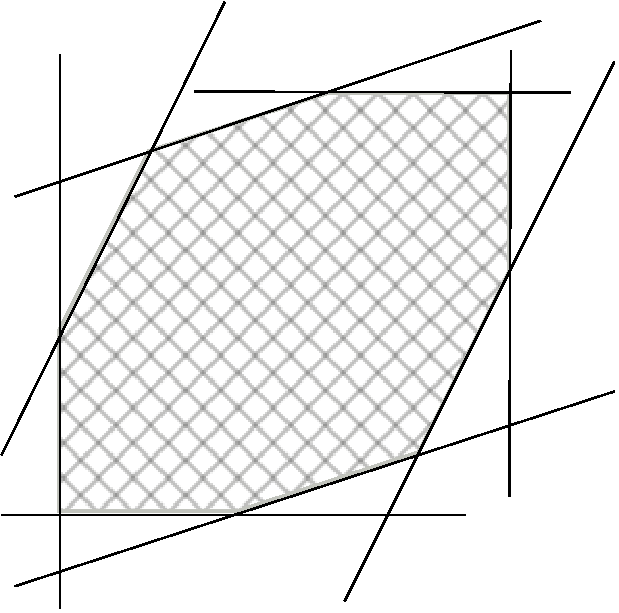
\includegraphics[trim={0 0 0 0},clip,width=0.75\linewidth]{img/chapter_2/zonotope_hyperplanes.pdf}
  \end{minipage}
  \caption{A zonotope can be represented by its vertices or its bounding hyperplanes. The vertex representation defines the zonotope as the convex hull of its vertices (including all interior and surface points). The hyperplane representation defines the zonotope as the intersection of half-spaces so that the direction of the half-space must be specified.}
  \label{fig:zonotope_vertices_hyperplanes}
\end{figure}

The process of retrieving zonotope vertices from its generator representation is a combinatorial problem known as the \emph{vertex enumeration problem}. The explicit enumeration of zonotope vertices is required in applications such as the fixed-rank integer quadratic program (\cite{ferrezSolvingFixedRank2005a}), signal processing (\cite{markopoulosOptimalAlgorithmsL_12014}), and linear regression models with interval data (\cite{cernyPossibilisticApproachLinear2013}).

Unfortunately, converting zonotope generators to vertices or bounding hyperplanes is a combinatorial problem. As the dimension or the number of generators increases, the number of vertices increases rapidly: Theorem 3.1 from (\cite{ferrezSolvingFixedRank2005a}) states that the number of vertices of an $n$-zonotope $\mathcal{Z}$ with $m$ generators is $\leq 2 \sum_{i=0}^{n-1} \binom{m-1}{i}$, with equality satisfied when the generators are in general position. For instance, a 3D zonotope can have up to $92$ vertices if it is defined by $10$ generators; $2452$ if it has $50$ generators; and $9902$ vertices for $100$ generators. Similarly, for an $n$-zonotope with $50$ generators, it has up to $39300$ vertices for $n=4$, more than $5.6\times 10^{14}$ for $n=25$, and more than $1.1\times 10^{15}$ for $n=50$. In a biomechanical context, considering the Stanford upper limb musculoskeletal model consisting of $50$ muscles and $7$ degrees-of-freedom (\cite{holzbaurModelUpperExtremity2005}), the torque feasible set has at most $32244452\approx 3.2\times 10^{7}$ vertices. Consequently, the required space to describe all the vertices becomes large very quickly, regardless of the efficiency of the enumeration algorithm. 

The following Section \ref{edge_enumeration_algorithm_section} presents a novel, efficient zonotope edge enumeration algorithm, called \emph{EdgeEnum}, which can be used to enumerate the vertices of a zonotope. Section \ref{time_complexity_edgeenum} shows that EdgeEnum is indeed theoretically \emph{efficient} by proving the polynomiality of both its time and space complexity when $n$ is fixed. An asymptotic growth comparison is also performed with various recent enumeration algorithms adapted to the zonotope vertex enumeration problem. Section \ref{time_benchmark} compares the time benchmarks of multiple algorithms and demonstrates that, in practice, \emph{exact} enumeration techniques may not be suitable when rapid evaluations of zonotopes are required, as we need for Chapters \ref{chapter:3} and \ref{chapter:4} for an optimization-based muscle personalization process. In this regard, Section \ref{sec:approximation_of_vertices_zonotope} offers some insights into the computation time of approximated vertex enumeration algorithms. Finally, Section \ref{conclusion_zonotope_enum_algorithm} summarizes the results and advantages offered by our approach, such as the ease of implementation and the potential for parallelism compared to existing methods, while highlighting the effectiveness of using vertices to describe zonotope characteristics of interest such as its global shape and orientation.

\section{The edge enumeration algorithm}
\label{edge_enumeration_algorithm_section}

While the main goal is to enumerate zonotope vertices, this section presents first an algorithm that enumerates the edges of a zonotope and then describes an edge-to-vertex conversion algorithm with negligible additional computation time. The edge enumeration algorithm takes as input the generator matrix of an $n$-zonotope $\Zono$ with $m$ generators in general position and returns a set of $m$-cube edges that map to the edges of $\Zono$.

Vertices do not contain information about other vertices, whereas edges are linked to at least two vertices. Therefore, knowledge of an edge allows for the description of its extremal vertices. This novel approach uses this information to make vertex enumeration faster by enumerating zonotope edges. Since a zonotope is the projection of a higher-dimensional cube, its edges are also the projection of some cube edges.

\subsubsection*{From cube edges to zonotope edges}
The construction of the edges of an $m$-dimensional hypercube, also called an $m$-cube, is an iterative process over dimensions 2 to $m$ (Figure \ref{fig:cube_edge_construction}). Starting from a square (or the 2-cube), each of its edges is embedded in 3D and then duplicated and translated by 1 along the newly created dimension.  New edges arise from this duplication: for each vertex $v$ in the previous step, a segment is created between $v$ and its newly duplicated and translated version $v'$. This process is iterated until the $m^{\text{th}}$ dimension is reached, at which point all of the $m$-cube edges are enumerated.

\begin{figure}[!htb]
  \captionsetup{justification=centering}
  \centering
  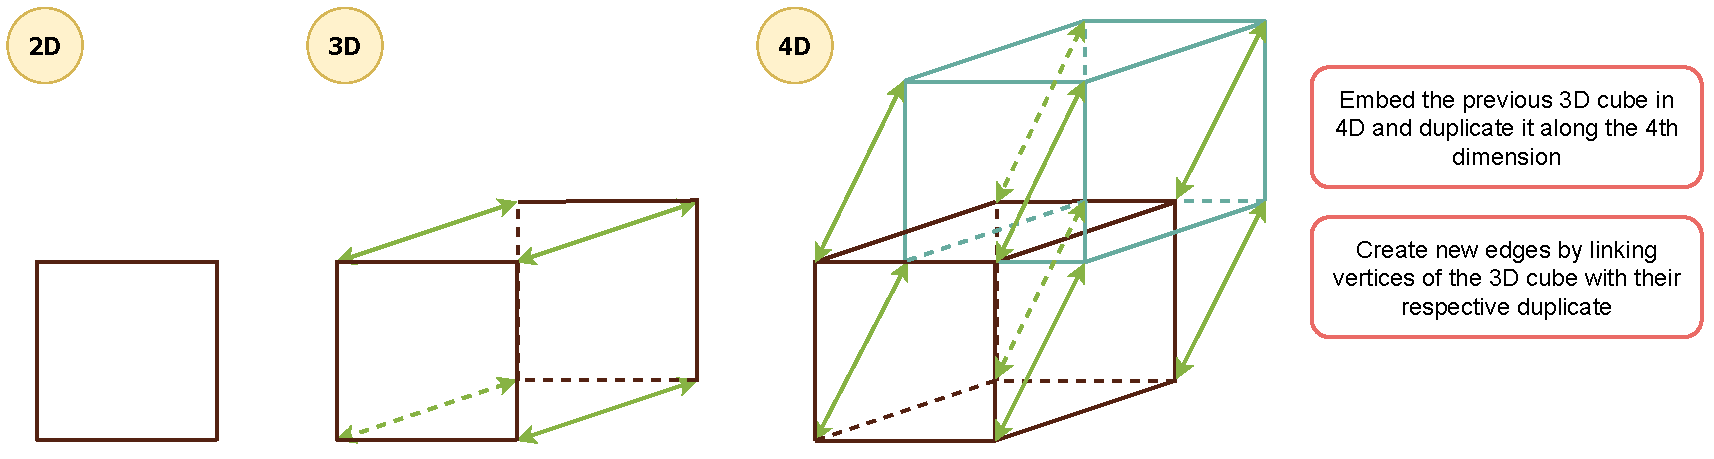
\includegraphics[trim={0 0 0 0},clip, width=1.0\linewidth]{img/chapter_2/zonotope_construction_from_cube_edge_duplication.pdf}
  \caption{Constructing the edges of a zonotope with $4$ generators requires constructing the edges of a $4$-dimensional hypercube. The process is iterative and starts from the square to retrieve the cube, then the $4$-cube. The creation of new edges arising at each new step is indicated by the green double arrows.}
  \label{fig:cube_edge_construction}
\end{figure}

Once all $m$-cube edges are enumerated, projecting them through the generator matrix of the zonotope yields a result similar to Figure \ref{fig:from_cube_edges_to_zonotope_edges}: a collection of line segments appear to encapsulate the zonotope.

\begin{figure}[!htb]
  \captionsetup{justification=centering}
  \centering
  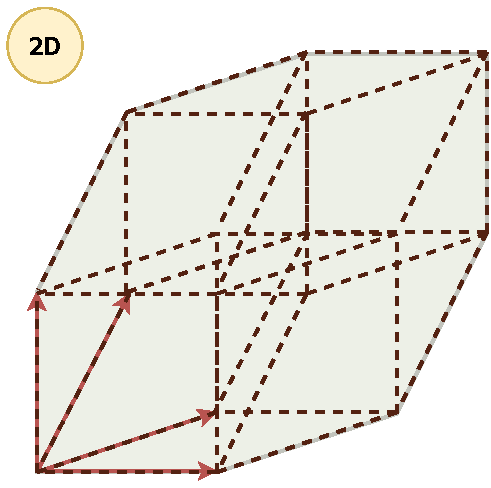
\includegraphics[trim={0 0 0 0},clip, width=0.3\linewidth]{img/chapter_2/zonotope_after_cube_duplication.pdf}
  \caption{Projecting the $4$-cube edges through the generator matrix of a 2D zonotope with $4$ generators.}
  \label{fig:from_cube_edges_to_zonotope_edges}
\end{figure}

This phenomenon is due to a parallelism property specific to zonotopes. Two segments or lines are \emph{parallel} if their direction vectors are collinear.

\begin{lemmabox}{Parallelism of zonotope edges with the generators}{zono_edges_parallel}
  For any $n$-dimensional zonotope $\Zono \subset \IRn$ with $m$ generators, each of its edges is parallel to one of its generators.

  Moreover, each projected edge of the $m$-cube is also parallel to one of the generators.
\end{lemmabox}
\begin{proof}
A linear or affine map preserves parallelism. 
Consider a zonotope $\Zono$ described by generators $\mathbf{g}_1,\dots,\mathbf{g}_m \in \IRn$ in general position. Let $G$ denote the generator matrix. If $n\geq 2$, then the edges of the $m$-cube clearly surject onto the zonotope edges.
The edges of the $m$-cube can be grouped by parallelism with a representing vector $\mathbf{r}_i = e_i \in \IRm$, where $e_i$ corresponds to the $i^{\text{th}}$ vector of the canonical basis of $\IRm$. Thus, $G\mathbf{r}_i = \mathbf{g}_i$. This ensures that when a cube edge is projected through $G$, it will necessarily be parallel to one of the generators.
\end{proof}

\begin{figure}[!htb]
      \captionsetup{justification=centering}
      \begin{minipage}{0.49\linewidth}
        \centering
        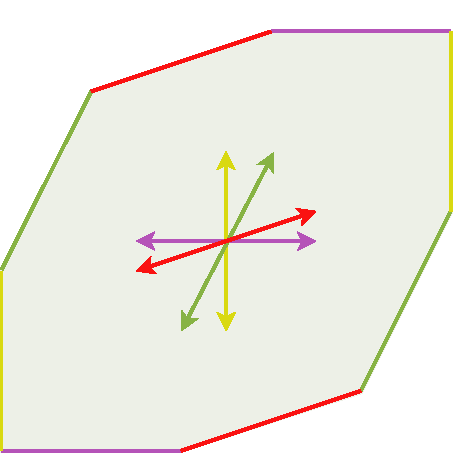
\includegraphics[trim={0 0 0 0},clip, width=0.55\linewidth]{img/chapter_2/zonotope_edges_parallel_generator.pdf}
      \end{minipage}
      \hfill
      \begin{minipage}{0.49\linewidth}
        \centering
        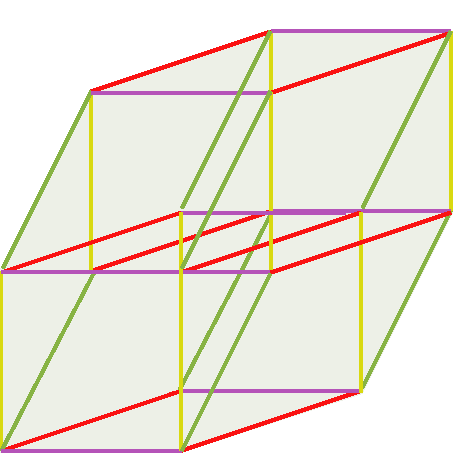
\includegraphics[trim={0 0 0 0},clip,width=0.55\linewidth]{img/chapter_2/zonotope_edges_parallel_generator_alt.pdf}
      \end{minipage}
      \caption{Left: Each edge of a zonotope $\Zono$ is parallel to one of its generators. Right: Projecting a $4$-cube edge through the generator matrix of $\Zono$ produces a line segment parallel to one of the generators.}
      \label{fig:zonotope_edges_parallel}
    \end{figure}
    
To enumerate the edges of a zonotope $\Zono(\mathbf{c}, G)$, a naive approach would be to first consider each edge $\mathbf{e}$ of an $m$-cube and project it through $\mathbf{e} \mapsto \mathbf{c} + G\mathbf{e}$. Then, after a selection process, only a relevant subset of these projected edges would be considered. However, this involves computing \emph{all} edges of an $m$-cube, which is not feasible due to the high combinatorics involved in the number of possible edges. Indeed, this would amount to $m2^{m-1}$ edges, which is greater than $2^m$, the number of its vertices (\cite{grunbaumConvexPolytopes2013}).

Our novel approach consists of using a straightforward elimination technique directly from the cube space, to remove unnecessary cube edges that do not project onto zonotope edges. The following paragraphs describe this process.

\subsubsection*{The convex hull of parallel lines}
As established in Lemma \ref{th:zono_edges_parallel}, each edge of a zonotope is parallel to one of its generators. Furthermore, each edge of the $m$-cube maps to a segment parallel to a generator. This allows for grouping the projected cube edges by parallelism, with a generator serving as the group representative. For each group, the extremal segments define the edges of the zonotope parallel to the considered generator.

Given these grouped projected edges, the next question is: \emph{how can we select only those on the zonotope surface?} While this is a challenging question for an arbitrary set of segments, the fact that we are working with projected edges parallel to a generator simplifies the problem.

This selection process is termed the \emph{convex hull of parallel lines}.  While convex hull algorithms are typically implemented for sets of points, the parallelism in this case allows for a modified approach that leverages the classic convex hull of points.

To illustrate this, consider a 2D example that generalizes to any dimension.  In the first iteration of the algorithm, the edges of a square are created, embedded in 3D, and projected through the submatrix of $G$ consisting of the first two columns. This results in three groups of edges, as shown by the edge colors in Figure \ref{fig:convex_hull_lines_intro}.

\begin{figure}[!htb]
  \captionsetup{justification=centering}
  
  \centering
  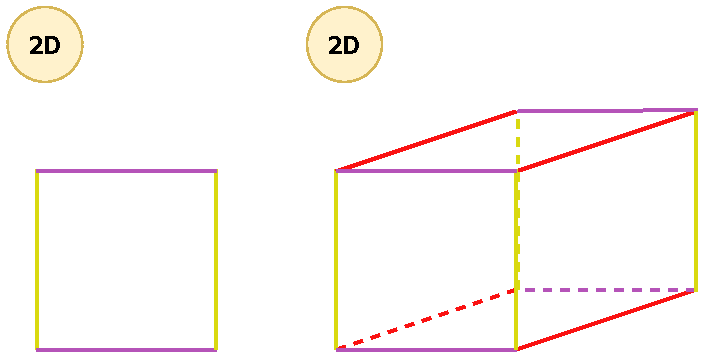
\includegraphics[trim={0 0 0 0},clip,width=0.5\linewidth]{img/chapter_2/zonotope_convex_hull_lines_intro.pdf}

  \caption{The edges on the right are created from embedding and duplicating the square edges to create a cube and then projecting them onto the plane through the first two columns of $G$.}
  \label{fig:convex_hull_lines_intro}
\end{figure}

Consider a group of parallel edges, such as the purple ones in Figure \ref{fig:convex_hull_lines_intro}, and extend them to lines. An arbitrary point is selected in the zonotope space and projected orthogonally onto each line. These projected points span a space of at most $n-1$ dimensions, where $n$ is the dimension of the zonotope. The convex hull operation is then applied to this set of projected points, and only the edges associated with points on the convex hull are retained (cf. Figure \ref{fig:convex_hull_lines}).

% \clearpage
\begin{figure}[!htb]
  \captionsetup{justification=centering}
  
  \centering
  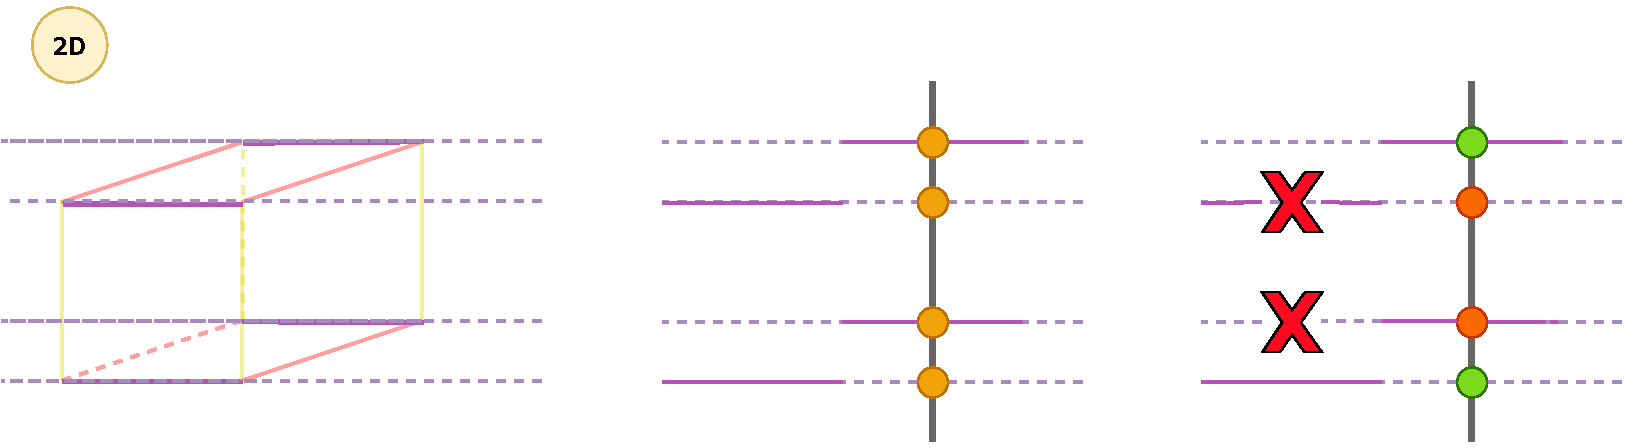
\includegraphics[trim={0 0 0 0},clip,width=1\linewidth]{img/chapter_2/zonotope_convex_hull_lines.pdf}

  \caption{From left to right: A group of parallel edges is selected and extended to lines. An arbitrary point is projected orthogonally onto these lines. The convex hull operation is applied to these points to retrieve the associated extremal edges. This works in any dimension, as long as a set of parallel lines is considered.}
  \label{fig:convex_hull_lines}
\end{figure}

This process is repeated for all groups of edges, which corresponds to the number of dimensions of the underlying hypercube, as shown in Figure \ref{fig:convex_hull_lines_repeat_groups}.

\begin{figure}[!htb]
  \captionsetup{justification=centering}
  
  \centering
  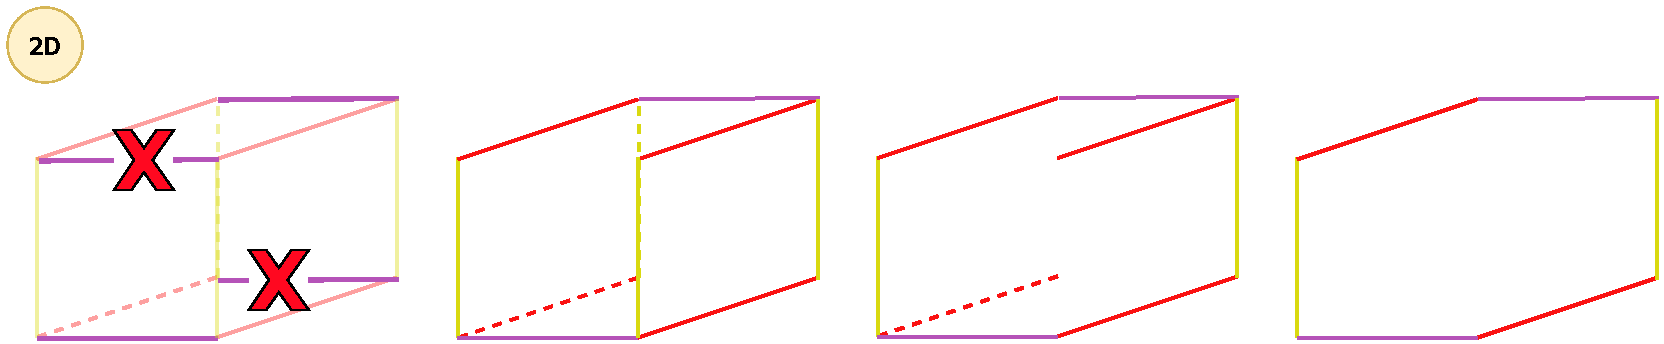
\includegraphics[trim={0 0 0 0},clip,width=1\linewidth]{img/chapter_2/zonotope_edge_elimination_repeat.pdf}

  \caption{Selection of the extremal edges for each group of parallel edges by applying the convex hull of parallel lines. First purple edges, then yellow, and finally red.}
  \label{fig:convex_hull_lines_repeat_groups}
\end{figure}

Once all groups have been processed, the remaining edges are precisely those needed to produce the edges of the zonotope generated by the first three columns of $G$. The embedding, duplication, and translation process is then employed to create the new edges in 4D, which are projected through the submatrix of $G$ consisting of the first four columns. The algorithm terminates when, after multiple iterations, the selected cube edges belong to the $m$-cube (cf. Figure \ref{fig:zonotope_edges_elimination_end}).

\begin{figure}[!htb]
  \captionsetup{justification=centering}
  
  \centering
  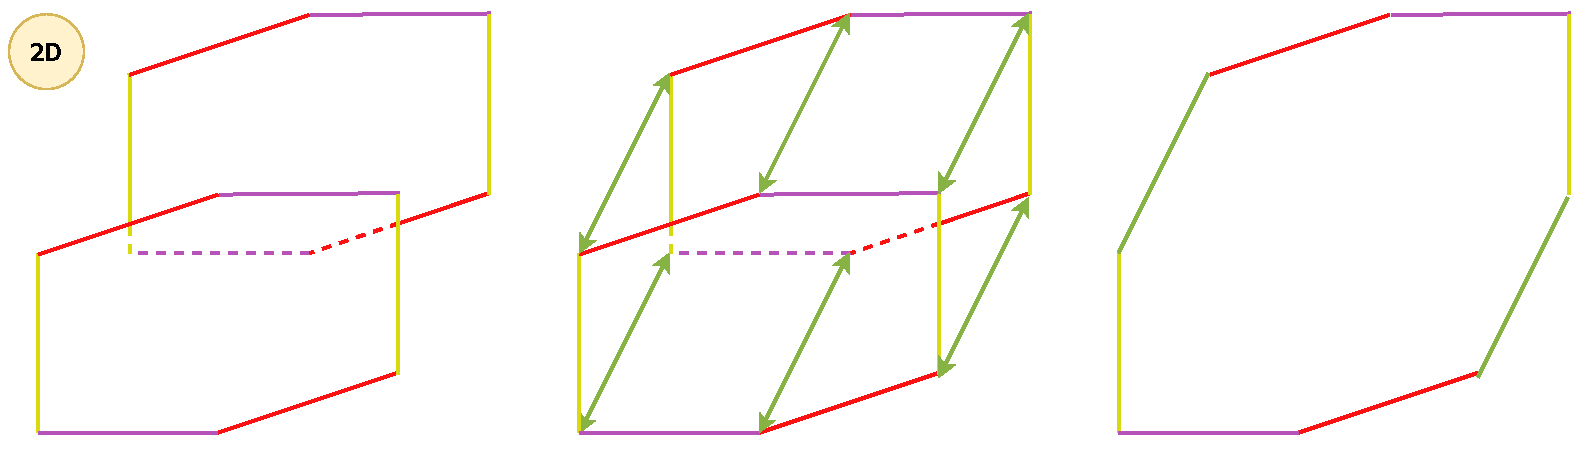
\includegraphics[trim={0 0 0 0},clip,width=1\linewidth]{img/chapter_2/zonotope_edges_elimination_end.pdf}

  \caption{After exactly $m-2$ iterations, the returned edges are precisely the zonotope edges.}
  \label{fig:zonotope_edges_elimination_end}
\end{figure}


\clearpage 
\subsubsection*{The EdgeEnum algorithm}

In the following algorithms, an edge of the $m$-cube is represented by two $m$-dimensional vectors: a direction vector and an initial position vector. Algorithm \ref{alg:cube_edge_enumeration} details the creation of a new set of edges in a higher dimension ($d+1$) from a given set of edges in $\mathbb{R}^d$, based on the construction of edges of a higher-dimensional cube. Algorithm \ref{alg:edge_enum}, called EdgeEnum, constructs zonotope edges following the reasoning described previously.

\begin{figure}[!ht]
  \centering
  \begin{minipage}{1.0\linewidth}
    \begin{algorithm}[H]
      \SetAlgoLined
      \KwData{$\textup{E}_d$, a set of edges in $\mathbb{R}^d$}
      \KwResult{$\textup{E}_{d+1}$, a set of edges in $\mathbb{R}^{d+1}$}
      
      \SetKwFunction{FMain}{duplicateAndLinkEdges}
      \SetKwProg{Fn}{Function}{:}{}
      \Fn{\FMain{$\textup{E}_d$}}{
        $\text{E}_{d+1} \gets \emptyset$\;
        \ForEach{$\mathbf{e}\in \textup{E}_d$}{
          $\mathbf{e}_0 \gets \textup{embedInOneHigherDimension}(\mathbf{e})$\;
          $\mathbf{e}_1 \gets \textup{translateAlongNewDimensionBy1}(\mathbf{e}_0)$\;
          $v_0^1,\, v_0^2 \gets \textup{verticesAtExtremities}(\mathbf{e}_0)$\;
          $v_1^1,\, v_1^2 \gets \textup{verticesAtExtremities}(\mathbf{e}_1)$\;
          $\mathbf{e}_{01}^1 \gets \textup{createEdge}(v_0^1, v_1^1)$\;
          $\mathbf{e}_{01}^2 \gets \textup{createEdge}(v_0^2, v_1^2)$\;
          $\text{E}_{d+1} \gets \text{E}_{d+1} \cup \{\mathbf{e}_0, \mathbf{e}_1, \mathbf{e}_{01}^1, \mathbf{e}_{01}^2\}$;
        }    
        \Return{$\textup{E}_{d+1}$}
      }
      \textbf{End Function}
      \caption{Duplication, translation, and linking of edges}
      \label{alg:cube_edge_enumeration}
    \end{algorithm}
  \end{minipage}
\end{figure}

\begin{figure}[!ht]
  \centering
  \begin{minipage}{1.0\linewidth}
    \begin{algorithm}[H]
      \SetAlgoLined
      \KwData{A matrix $N \in \mathbb{R}^{n\times m}$, with $n\geq 2$ and $m\geq 2$}
      \KwResult{Edges of the zonotope $\Zono(\mathbf{c}, N)$}
      $d\gets 2$\;
      $N_d\gets N[:,:d]$\;      
      $\text{Edges}(\Cube_d)\gets \{\text{edges of the 2D cube}\}$ \tcp*{where $\Cube_d$ is the cube $[0,1]^d$.}
      $\text{Edges}(\Zono(\mathbf{c}, N_d))\gets \{\mathbf{c} + N_d\mathbf{e} \mid \mathbf{e}\in\text{Edges}(\Cube_d)\}$ \;
      
      $d\gets 3$\;
      \While{$d \leq m$}{
        $N_d\gets N[:,:d]$\;
        $\text{Edges}(\Cube_{d-1}) \gets \text{Edges}(\Cube_d)$\;
        $\textup{Edges}(\Cube_{d}) \gets \textup{duplicateAndLinkEdges}(\textup{Edges}(\Cube_{d-1}))$ \tcp*{cf. Algorithm \ref{alg:cube_edge_enumeration}}
        
        $\text{Edges}(\Zono(\mathbf{c}, N_d))\gets \{\mathbf{c} + N_d\mathbf{e} \mid \mathbf{e}\in\text{Edges}(\Cube_d)\}$ \;
    
        \ForEach{group of parallel edges $G\in\textup{Edges}(\Zono(\mathbf{c}, N_d))$}{
          \ForEach{$\mathbf{c} + N_d\mathbf{e} \notin \textup{ext}(\textup{conv}(G))$}{
            $\text{Edges}(\Cube_d) \gets \text{Edges}(\Cube_d) / \{\mathbf{e}\}$\;
          }
          
        }
        
        $d\gets d+1$
      }
      
      $\text{Edges}(\Zono(\mathbf{c}, N_d))\gets \{\mathbf{c} + N_d\mathbf{e} \mid \mathbf{e}\in\text{Edges}(\Cube_d)\}$ \;
      \Return{$\textup{Edges}(\Cube_d),\, \textup{Edges}(\Zono(\mathbf{c}, N_d))$}
      \caption{EdgeEnum: zonotope edge enumeration algorithm}
      \label{alg:edge_enum}
    \end{algorithm}

  \end{minipage}
\end{figure}

\section{Theoretical complexity}
\label{time_complexity_edgeenum}
This section presents various theoretical results about the new algorithm, using computational complexity as the primary tool for comparison. While a thorough analysis of time and space complexity is provided, the primary focus is on the asymptotic time growth as the number of generators increases, as this relates to a larger number of muscles considered when computing the torque feasible set. Therefore, $n$, the dimension of the ambient space of the zonotope, is considered to be fixed, while the number of generators, $m$, is assumed to be large.

Before delving into the analysis, let's review some basic concepts related to algorithmic complexity and asymptotic growth:

\paragraph*{Asymptotic Growth and Big O Notation.} Asymptotic growth describes the behavior of a function as its input becomes very large. The Big O notation denotes the dominant terms of a function. For instance, the function $f\colon \mathbb{N} \rightarrow \mathbb{N}$ defined by $f(n) = 4n^5 + n^5\log (n)$ is dominated by the term $n^5\log(n)$. This means that as $n$ tends to $+\infty$, $f(n)$ will have approximately the same growth rate as the function $n\mapsto n^5\log(n)$. The Big O notation expresses this comparison by stating that $f$ is in $O(n^5\log(n))$ or $f(n) = O(n^5\log(n))$. To compare the asymptotic growth of two functions, their respective growth rates are calculated, and the ratio of these rates is evaluated to determine which function has slower growth. If the ratio tends to a constant value, then both functions have asymptotically the same growth. More generally, $O$ represents a class of functions bounded by a given formula. In the example above, $f$ is \emph{in} $O(n^5\log(n))$, but it is also in higher classes such as $O(n^6)$ or $O(n^{20})$.

\paragraph*{Algorithmic Complexity.} Two types of complexity are commonly used to describe algorithms: \emph{time} complexity and \emph{space} complexity. Time complexity theoretically evaluates the time required for each operation, while space complexity evaluates the required storage.

\paragraph*{Efficient Algorithm.} An algorithm is \emph{polynomial} or \emph{efficient} if its time complexity is upper bounded by a polynomial expression of both the input size and the output size (\cite{fukudaZonotopeConstructionMinkowski2004a}). In other words, the running time of the algorithm does not grow exponentially as the input size increases, making it generally efficient for solving problems. For algorithms related to zonotope vertex enumeration, the input size corresponds to the number of dimensions times the number of generators (essentially the number of elements in the generator matrix), while the output size includes the number of vertices, faces, and generator dimensions.

\paragraph*{Compact Algorithm.} An algorithm is \emph{compact} if its space complexity is polynomial in the input size. This means that a compact algorithm does not store \emph{all} of the output and can stream the results directly without storing the entire output. This is a valuable property, especially when the output size is large. In the literature, two main approaches can be found: reverse-search-based algorithms and iterative algorithms. Algorithms are theoretically more valuable if they are compact, especially in high dimensions, so this approach is preferred and commonly found (\cite{avisPivotingAlgorithmConvex}; \cite{guCounterfactualIdentificationLatent2022}; \cite{radaNewAlgorithmEnumeration2018}). However, non-compact algorithms should not be excluded, depending on the application context.

\paragraph*{Optimal Algorithm.} An algorithm is \emph{optimal} (in time and/or in space) if its complexity has been proven to be the lowest possible. For instance, Theorem 3.2 in (\cite{ferrezSolvingFixedRank2005a}) states that a time-optimal algorithm exists that enumerates all zonotope vertices in time $O(m^{n-1})$, which was implemented in (\cite{edelsbrunnerConstructingArrangementsLines1983}). However, such an optimal algorithm may not be practical (\cite{ferrezSolvingFixedRank2005a}). First, it uses an incremental strategy that requires storing all extreme points of a subproblem based on a smaller number of generators. Second, it is complex to implement and needs to store all faces and their incidence (i.e., whether the intersection of two faces is another face). In other words, Edelsbrunner et al.'s algorithm is time-optimal and efficient but space-inefficient.

This work focuses primarily on time efficiency. As the following theorems demonstrate, the new algorithm is time-efficient, even when considering the edge-to-vertex transition. It is also space-efficient but not compact.

Before analyzing the complexity, let us introduce a useful result concerning the number of specific faces in a zonotope. A zonotope $\Zono$ in dimension $n$ has $n-1$ types of faces: the $0$-faces are called \emph{vertices}, the $1$-faces \emph{edges}, the $(n-2)$-faces \emph{ridges}, and the $(n-1)$-faces \emph{facets}. In specific cases, such as in dimension 2, the edges correspond to the facets. In 3D, edges correspond to ridges.

\begin{lemmabox}{Upper bound on the number of $k$-faces of a zonotope}{nb_k_faces_zonotope}
  For $G\in\IRnm$, the number of $k$-faces of the zonotope $\Zono(G)$ for $k=1,\dots, n-1$ is upper bounded by $f_k(\Zono)$, where
  \[f_k(\Zono) = 2\binom{m}{k} \sum_{i = 0}^{n-k-1} \binom{m-k-1}{i}.\]
  This bound is attained if $\Zono$ is in general position.
\end{lemmabox}
\begin{proof}
  This result, with proof, can be found in (\cite{fukudaZonotopeConstructionMinkowski2004a}; \cite{donohoCountingFacesRandomlyProjected2010}; \cite{grunbaumConvexPolytopes2013}).
\end{proof}

\subsection{Time complexity}
\begin{theorembox}{Time complexity of EdgeEnum}{time_complexity}
  For an $n$-zonotope $\Zono$ with $m$ generators in general position, the edge enumeration algorithm has time complexity
  \[O\left( nm^2f_1(\Zono)\right),\]
  where $f_1(\Zono)$ denotes the number of edges of $\Zono$.
\end{theorembox}
\begin{proof}
    Each iteration of the algorithm (i.e., $d=3,\dots, m$) considers a new zonotope $\Zono_d$ generated by the first $d$ columns of the generator matrix $G\in\IRnm$ and constructs its edges based on the set of edges of $\Zono_{d-1}$. The following is a thorough analysis of the computation time of each step in the algorithm:

    \textbf{1. Embed, duplicate, and translate Edges:} In the first inner loop, a new dimension is added to the edges of $\Zono_{d-1}$. This is achieved by concatenating a $0$ to both the direction and position vectors that describe each edge. These embedded edges are then duplicated, and the copied versions have their direction and position last coordinates mutated to $1$. New edges are created by linking the corresponding extremity points from the embedded edges to their translated counterparts. This entire step can be performed in $O(1)$ time complexity for each substep, within a loop over each of the previous edges, resulting in $O(f_1({\Zono_{d-1}}))$ time complexity.

    \textbf{2. Group edges by parallelism:} The newly created set of edges consists of exactly $4f_1(\Zono_{d-1})$ edges. Since collinearity between cube edges is preserved under linear transformation, grouping edges of zonotope $\Zono_d$ by parallelism only requires grouping the cube edges by their directions. Using a dictionary structure in Python, this grouping process has a time complexity of $O(f_1(\Zono_{d-1}))$.
    
    \textbf{3. Apply the convex hull to each group of edges:} Each group of edges consists of $2f_1(\Zono_{d-1}) / (d-1)$ edges, and there are $d$ groups. For each group, each edge is projected onto $\IRn$ through the generator matrix of $\Zono_d$. This corresponds to one matrix-vector operation with a time complexity of $O(nd)$ per edge. After the projection, the orthogonal projection of the origin in $\IRn$ onto the line spanned by the projected edge is computed in $O(n)$ time complexity (the dimension of the ambient space where the line is defined). The convex hull of the projected edges is then computed as the convex hull of the orthogonal projections of the origin onto the lines spanned by the edges. Consider the time complexity of Chan's convex hull algorithm in $n$ dimensions. It is an output-sensitive algorithm, meaning its complexity depends on the size of the output. Its time complexity is $O(n_v\log h)$, with $n_v$ being the number of given points and $h$ the number of points on the convex hull. Since the zonotope $\Zono_d$ is in general position, the number of edges in each group is $f_1(\Zono_d) / d$. The total time complexity of step 3 is then of order 
    $d (\frac{2f_1(\Zono_{d-1})}{d-1}nd + \frac{2f_1(\Zono_{d-1})}{d-1}n + \frac{2f_1(\Zono_{d-1})}{d-1}\log(\frac{f_1(\Zono_{d})}{d}))$, which is
    $O(f_1(\Zono_{d-1}) nd +f_1(\Zono_{d-1})  \log(f_1(\Zono_{d}) / d))$.

    After $d$ iterations, the complexity is of order $\sum_{d=3}^m f_1(\Zono_{d-1}) nd +  f_1(\Zono_{d-1}) \log(f_1(\Zono_d) / d)$ and since $d \leq m$ and $f_1(\Zono_d) \leq f_1(\Zono)$, we have the following upper bound:
    \begin{align*}
        \sum_{d=3}^m f_1(\Zono_{d-1}) nd +  f_1(\Zono_{d-1}) \log(f_1(\Zono_d) / d) &\leq  f_1(\Zono) \left[ n \sum_{d=3}^m d + \sum_{d=3}^m \log\left(\frac{f_1(\Zono)}{d}\right) \right] \\
        &\leq  f_1(\Zono) \left[ nm\frac{m+1}{2} +  \log\left(\prod_{d=1}^m\frac{f_1(\Zono)}{d}\right) \right] \\
        &\leq  f_1(\Zono) \left[ n\frac{m^2+m}{2} +  \log\left(\frac{f_1(\Zono)^m}{m!}\right) \right]
    \end{align*}
    So the edge-based algorithm is upper bounded in $O\left( nm^2f_1(\Zono) +  f_1(\Zono)\log\left(\frac{f_1(\Zono)^m}{m!}\right)\right)$.

    The next step is to show that $nm^2f_1(\Zono)$ is the dominant term in this upper bound. This is done by demonstrating that for any growth of $n$ and $m$, the expression 
    $$f_1(\Zono)\log\left(\frac{f_1(\Zono)^m}{m!}\right) / (nm^2f_1(\Zono))$$
    is upper-bounded by a function whose growth tends to be constant (meaning it is $O(1)$).
    \begin{align*}
        \frac{f_1(\Zono)\log\left(\frac{f_1(\Zono)^m}{m!}\right)}{nm^2f_1(\Zono)} 
        &\leq \frac{1}{nm^2}\log\left(f_1(\Zono)^m\right) \\
        &= \frac{1}{nm}\log\left(f_1(\Zono)\right) \\
        &= \frac{1}{nm} \log\left(2\binom{m}{1}\sum_{i=0}^{n-2}\binom{m-2}{i}\right),\quad \text{using theorem \ref{th:nb_k_faces_zonotope}} \\
        &\leq \frac{1}{nm} \log\left(m2^{m-1}\right),\quad \text{using } \sum_{i=0}^{n-2}\binom{m-2}{i} \leq \sum_{i=0}^{m-2}\binom{m-2}{i} = 2^{m-2}  \\
        &= \frac{ \log(m)}{nm} + \frac{ (m-1)\log(2)}{nm} \\
    \end{align*}
    There are now three cases to study:
    \begin{enumerate}[noitemsep]
        \item {$n \rightarrow +\infty$ and $m$ grows at a smaller rate than $n$ ($\lim_{m,n\to +\infty}\frac{m}{n} = 0$): 
        $$\lim_{m,n\to +\infty}\frac{ \log(m)}{nm} = \lim_{m,n\to +\infty}\frac{1}{nm}  = 0\quad \text{and} \quad \lim_{m,n\to +\infty} \frac{ (m-1)\log(2)}{nm} = \lim_{n\to +\infty}\frac{1}{n}  =  0$$
        }
        \item  {$m \rightarrow +\infty$ and $n$ grows at a smaller rate than $m$ ($\lim_{m,n\to +\infty}\frac{n}{m} = 0$): 
        $$\lim_{m,n\to +\infty}\frac{ \log(m)}{nm} = \lim_{m,n\to +\infty}\frac{1}{nm}  = 0\quad \text{and} \quad \lim_{m,n\to +\infty} \frac{ (m-1)\log(2)}{nm} = \lim_{m,n\to +\infty}\frac{1}{n}  =  0$$
         }
         \item  {$m \rightarrow +\infty$ and $n \rightarrow +\infty$ at an equivalent rate ($\lim_{m,n\to +\infty}\frac{n}{m} = C$, for $C$ a positive constant): 
         $$\lim_{m,n\to +\infty}\frac{ \log(m)}{nm} = \lim_{m,n\to +\infty}\frac{1}{nm}  = 0\quad \text{and} \quad \lim_{m,n\to +\infty} \frac{ (m-1)\log(2)}{nm} = \lim_{m,n\to +\infty}\frac{1}{n}  =  0$$
          }
    \end{enumerate}
    All cases confirm that the growth of $f_1(\Zono)\log\left(\frac{f_1(\Zono)^m}{m!}\right)$ is dominated by the growth of  $nm^2f_1(\Zono)$ for any growth of $m$ and $n$. Therefore, the complexity of the edge enumeration algorithm is $O(nm^2f_1(\Zono))$.
\end{proof}

The following intermediate result will be used in the proof of Theorem \ref{th:time_complexity_n_fixed}.
\begin{lemmabox}{Asymptotic upper bound for the number of $k$-faces}{big_O_nb_k_faces} 
For a zonotope $\Zono$ in dimension $n$ with $m$ generators in general position, the number of $k$-faces of $\Zono$, denoted by $f_k(\Zono)$, has an asymptotic growth upper-bounded by $O(m^{n-1})$ when $k$ and $n$ are fixed, and $m$ is large.
\end{lemmabox}

While it is well-known that the number of vertices $f_0(\Zono)$ is asymptotically bounded by $O(m^{n-1})$ (proven in (\cite{zaslavskyFacingArrangementsFaceCount1975})), this lemma extends this result to higher dimensions to provide an asymptotic upper bound for the number of $k$-faces when $k$ and $n$ are constant. This implies that the number of vertices, edges, ridges, hyperplanes, and all types of $k$-faces of a general zonotope are all upper bounded by the same type of growth as $m$ increases. This lemma will be used later to compute the asymptotic growth of the edge enumeration algorithm when $n$ is fixed, which will facilitate comparison with existing algorithms.
\begin{proof}
    The proof proceeds by finding an upper bound for $f_k(\Zono)$ that is $O(m^{n-1})$ for fixed $n$. First, note that for $0\leq n\leq m$, $m^n$ is an upper bound for $\binom{m}{n}$:
    \begin{align}
    \label{ineq:upper_bound_binomial}
    \binom{m}{n} &= \frac{m!}{n!(m-n)!} = \frac{1}{n!} \cdot m(m-1)(m-2)\dots (m-n+1) \leq m^n.
    \end{align}
      
    Also, when $m$ is large, and $k, n$ are fixed, it is reasonable to assume that $(n-k-1) \leq (m-k-1)/2$, so
    \begin{align}
    \label{ineq:upper_bound_binomial_half}
    \binom{m-k-1}{i}\leq \binom{m-k-1}{n-k-1},\quad \text{for any $i = 1, \dots, n-k-1$}.
    \end{align}
      
    Hence, the following holds:
    \begin{align*}
    f_k(\Zono) &= 2\binom{m}{k}\sum_{i=0}^{n-k-1} \binom{m-k-1}{i} \\
    &\leq 2\binom{m}{k}\ \sum_{i=0}^{n-k-1} \binom{m-k-1}{n-k-1},\quad \text{using inequality \eqref{ineq:upper_bound_binomial_half}} \\
    &\leq 2m^k (m-k-1)^{n-k-1} (n-k),\quad \text{using inequality \eqref{ineq:upper_bound_binomial}}.
    \end{align*}
    The last inequality is equivalent to stating that $f_k(\Zono)$ is $O(m^{n-1})$ for fixed $k$ and $n$, and large $m$.
\end{proof}

\begin{theorembox}{Time complexity of EdgeEnum when $n$ is fixed}{time_complexity_n_fixed}
    If $n$ is fixed, and $m$ is large, the time complexity of the edge enumeration algorithm is $O(m^{n+1})$. Therefore, EdgeEnum is a polynomial-time algorithm for a fixed $n$.
\end{theorembox}
\begin{proof}
    This follows directly from Lemma \ref{th:big_O_nb_k_faces}, which states that the number of edges $f_1(\Zono)$ is $O(m^{n-1})$ when $n$ is fixed. Using the time complexity of EdgeEnum from Theorem \ref{th:time_complexity}, we have for fixed $n$: $O(nm^2f_1(\Zono)) = O(m^2m^{n-1}) = O(m^{n+1})$.
\end{proof}

\subsubsection*{From edges to vertices}
\begin{theorembox}{Time complexity of converting Edges to vertices}{time_complexity_edge_to_vertex}
    For an $n$-zonotope $\Zono$ with $m$ generators in general position, the time complexity of an algorithm that enumerates vertices from its edges is $O(nmf_1(\Zono))$.
\end{theorembox}
\begin{proof}
Every edge of $\Zono$ is linked to two vertices, which correspond to its extremities. The transformation of all edges to vertices can be performed with a time complexity of $O(f_1(\Zono)nm)$. Indeed, the two extremities of each cube edge must be projected through the generator matrix, which accounts for $2f_1(\Zono)nm$ $O(1)$ steps. An iteration over all these vertices can also be performed to ensure the uniqueness of each vertex, as two edges can lead to a common vertex. This verification step can be done in $O(f_1(\Zono))$ time complexity in Python using a hash structure.
\end{proof}
    
Since $nm^2f_1(\Zono)$ dominates $nmf_1(\Zono)$, the conversion step from edges to vertices does not have a theoretical impact on the time complexity in a worst-case scenario when added after the edge enumeration algorithm.

\subsection{Space complexity}
\begin{theorembox}{Space complexity of EdgeEnum}{space_complexity}
    For an $n$-zonotope $\Zono$ with $m$ generators in general position, the edge enumeration algorithm has space complexity 
    \begin{align*}
        O(n^2m^2f_1(\Zono))
    \end{align*}
    where $f_1(\Zono)$ denotes the number of edges of $\Zono$.
\end{theorembox}
\begin{proof}
    The algorithm starts with a matrix in $\IRnm$, so it requires an input space of $O(nm)$. In the first steps, the definition of the $2$-cube edges and their projection clearly require $O(n)$ space.

    \textbf{1. Embed, duplicate, and translate edges:} 
    A cube edge can be described in two parts: a direction and a position in $\IRm$. A direction of a cube edge requires $O(1)$ space since it is equivalent to a vector $e = (0, \dots, 0, 1, 0,\dots, 0) \in \IRm$ (due to the parallelism of edges to the canonical basis of $\IRm$). However, the position can be more general, so let's consider a worst-case scenario of $O(m)$ space.

    Each edge at the beginning of the loop is copied, embedded, duplicated, and new edges are created. There are at most $f_1(\Zono_{d-1})$ edges at the beginning, so these steps require a space of $O((d-1)\cdot f_1(\Zono_{d-1}) + 3\cdot d\cdot f_1(\Zono_{d-1})) = O(d\cdot f_1(\Zono_{d-1}))$.

    \textbf{2. Group edges by parallelism:} 
    First, all newly created edges need to be projected onto the space generated by $N_d$, resulting in a new set of projected edges requiring $O(ndf_1(\Zono_{d-1}))$ space. Using a dictionary in Python to pair edges with a projected direction (in this case, corresponding to a generator of $N_d$) requires $O(d)$ space, where $d$ is the number of generators in the current iteration. Thus, the total space required in this step is $O(ndf_1(\Zono_{d-1}))$.
    
    \textbf{3. Apply the convex hull to each group of edges:} For each of the $d$ groups of edges (consisting of $O(nf_1(\Zono_{d-1}))$ edges), Chan's convex hull algorithm has a space complexity of $O(n\cdot nf_1(\Zono_{d-1})) = O(n^2 f_1(\Zono_{d-1}))$. This leads to a total space complexity of $O(dn^2f_1(\Zono_{d-1}))$.

    In conclusion, since $d\leq m$ and $f_1(\Zono_d) \leq f_1(\Zono_m)$, the space complexity for all the loops is $O(nm + n + \sum_{d=3}^m df_1(\Zono_{d-1}) + ndf_1(\Zono_{d-1}) + dn^2f_1(\Zono_{d-1}))$. Since the terms in the sum are dominated by $dn^2f_1(\Zono_{d-1})$, which is itself dominated by $mn^2f_1(\Zono_d)$, the total space complexity is $O(n^2 m^2 f_1(\Zono_d))$.
\end{proof}

This leads directly to the following result:

\begin{theorembox}{Space complexity of converting edges to vertices}{space_complexity_edge_to_vertex}
    For an $n$-zonotope $\Zono$ with $m$ generators in general position, the space complexity of an algorithm that enumerates vertices from its edges is $O(nf_1(\Zono))$.
\end{theorembox}
\begin{proof}
    Consider $f_1(\Zono)$, the maximum number of edges of a zonotope $\Zono$. The input of the conversion algorithm thus requires $O(nf_1(\Zono))$ space, which is represented as a dictionary with a zonotope generator and a position vector in $\IRn$. For each of these edges, the extremal vertices are created, which include the position vector and the addition of the position vector and the associated generator. Therefore, the space complexity remains $O(nf_1(\Zono))$.
\end{proof}

This ensures that the total space complexity from edge enumeration to vertex enumeration is $O(n^2m^2f_1(\Zono))$.

\begin{theorembox}{Space complexity of EdgeEnum when $n$ is fixed}{space_complexity_n_fixed}
    If $n$ is fixed, and $m$ is large, the space complexity of the edge enumeration algorithm is $O(m^{n+1})$. Therefore, EdgeEnum is a polynomial-space algorithm for fixed $n$.
\end{theorembox}
\begin{proof}
    The space complexity is $O(n^2m^2f_1(\Zono))$, and $f_1(\Zono)$ is $O(m^{n-1})$ when $n$ is fixed. Thus, $O(n^2m^2f_1(\Zono))$ is $O(m^{n+1})$, which is a polynomial bound for both the input size $nm$ and the output size $O(m^{n-1})$.
\end{proof}

\subsection{Time-theoretic comparison with other algorithms}

The proposed algorithm exhibits a time complexity of $O(m^{n+1})$, while the optimal lower bound is $O(m^{n-1})$. Despite this discrepancy, the algorithm demonstrates several desirable properties, such as being easily implementable with standard scientific programming languages and packages. Nevertheless, other significant algorithms focus on this problem, which will be described succinctly below.

\paragraph*{Avis and Fukuda's pivoting algorithm (\cite{avisPivotingAlgorithmConvex}).}

The \emph{pivoting} algorithm, a type of \emph{reverse-search} algorithm created by the same authors, was initially designed to enumerate the vertices of a polytope described by a set of inequalities. Broadly, the algorithm starts with a vertex, and then a neighboring vertex is found using a \emph{pivot rule}, which decides which vertex to visit next based on the current vertex and the polytope structure. The new vertex is then marked as visited, and through iteration over each newly found vertex, all polytope vertices are enumerated. Numerous variants of this algorithm are possible by adapting the pivot rule. This algorithm has also been extended to compute vertices of a zonotope using only its generators and has been implemented in C++ with a Python wrapper in \emph{libzonotope} (\cite{yngvassonLibzonotope}). Additionally, an effective parallelized variant of the pivoting algorithm was developed (\cite{weibelImplementationParallelizationReverseSearch2010}) and can be used through the C++ implementation \emph{Minksum} (\cite{weibelMinksum}).

The initial reverse-search algorithms were not described as zonotope vertex enumeration algorithms. 
They were implemented to solve two kinds of problems: computing the convex hull of a set of points and computing the \emph{cell enumeration of a central hyperplane arrangement problem}. 
The latter corresponds to an alternative description of a zonotope. There is a one-to-one correspondence between the combinatorial face structure of a zonotope and its central hyperplane arrangement. The idea is to consider the hyperplanes normal to each generator of a zonotope: the \emph{cells} of this arrangement correspond to the regions created by the hyperplanes' intersections. Describing and enumerating these cells (via a sign vector as shown in (\cite{ferrezSolvingFixedRank2005a,radaNewAlgorithmEnumeration2018})) is equivalent to finding the vertices of a zonotope. Figures \ref{fig:zonotope_hyperplane_arrangement} and \ref{fig:zonotope_hyperplane_arrangement2} summarize this correspondence by providing some intuition on how to construct it from a zonotope and how to compute vertices from the regions of such an arrangement. This construction generalizes well for zonotope generators in any dimension. 
For a deeper understanding of this duality and further details on this correspondence, the reader is invited to consult the \emph{Duality} section of (\cite{ferrezSolvingFixedRank2005a}), or more generally, the dedicated chapter \emph{Arrangement of hyperplanes} in (\cite{grunbaumConvexPolytopes2013}).

\begin{figure}[!htb]
      \captionsetup{justification=centering}
      \begin{minipage}{0.49\linewidth}
        \centering
        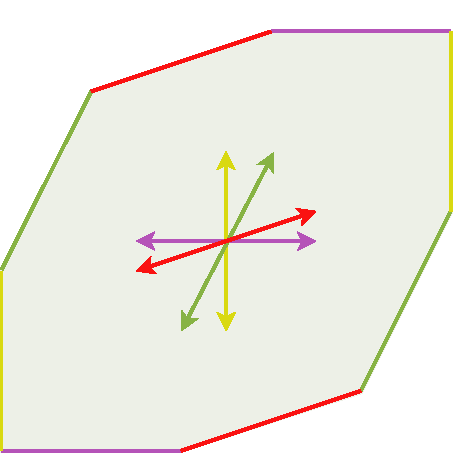
\includegraphics[trim={0 0 0 10},clip, width=0.6\linewidth]{img/chapter_2/zonotope_edges_parallel_generator.pdf}
      \end{minipage}
      \hfill
      \begin{minipage}{0.49\linewidth}
        \centering
        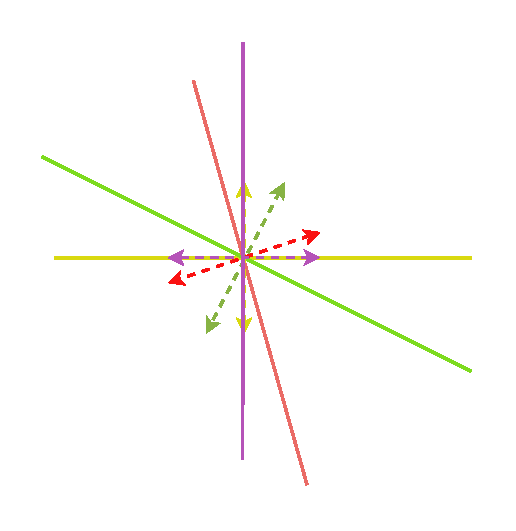
\includegraphics[trim={10 50 10 50},clip,width=0.8\linewidth]{img/chapter_2/central_arrangement.pdf}
      \end{minipage}
      \caption{Left: A zonotope with four generators. Right: The hyperplanes normal to each generator. This corresponds to its \emph{central hyperplane arrangement}.}
      \label{fig:zonotope_hyperplane_arrangement}
    \end{figure}
    
    \begin{figure}[!htb]
      \captionsetup{justification=centering}
      \centering
      
      \begin{minipage}{0.49\linewidth}
        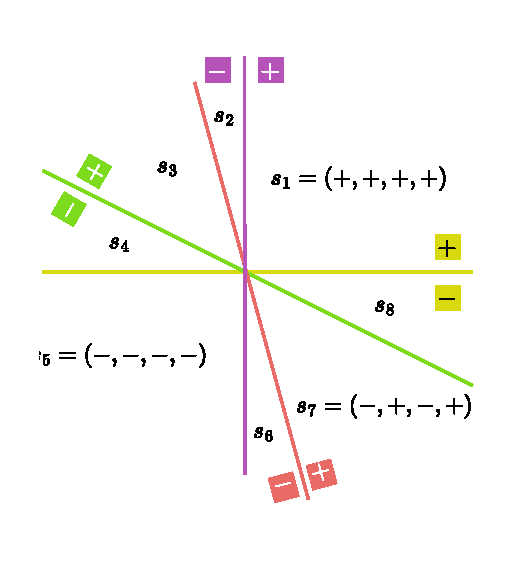
\includegraphics[trim={0 20 0 20},clip, width=0.9\linewidth]{img/chapter_2/sign_vectors_zonotope.pdf}
      \end{minipage}
      \hfill
      \begin{minipage}{0.49\linewidth}
        \hfill
        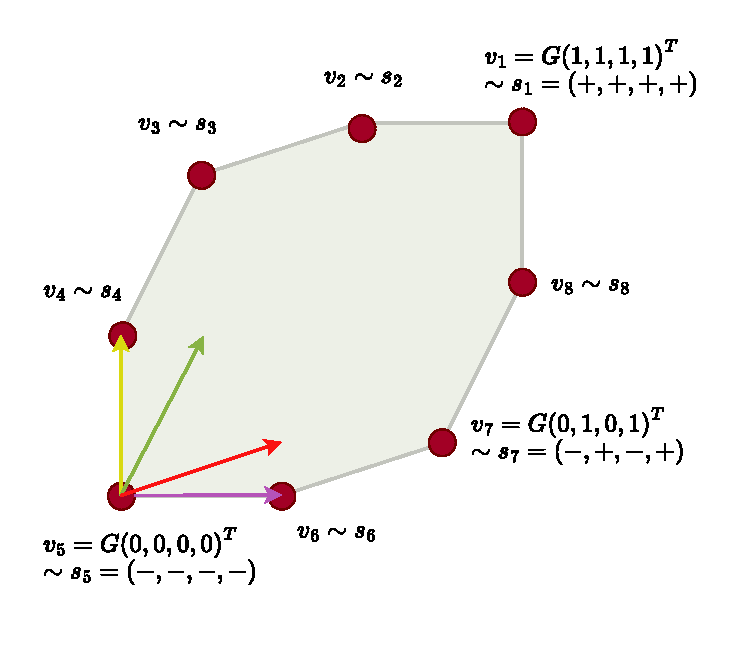
\includegraphics[trim={0 20 0 20},clip,width=1\linewidth]{img/chapter_2/zonotope_vertices_sign_vectors.pdf}
      \end{minipage}
      \caption{Let $G$ be the matrix with the yellow, purple, red, and green generators. In its central hyperplane arrangement, each region (or \emph{cell}) is represented by a sign vector $s_i$. Any $n$-dimensional space can be separated into exactly two half-spaces by a hyperplane. There are exactly as many cells as vertices in the underlying zonotope. Moreover, they are in one-to-one correspondence, as shown by the symbol $\sim$.}
      \label{fig:zonotope_hyperplane_arrangement2}
    \end{figure}

Due to the simplicity of working with sign vectors, there is a focus in computational geometry on creating algorithms dedicated to enumerating the cells of central hyperplane arrangements. Recent algorithms include those detailed in (\cite{radaNewAlgorithmEnumeration2018}), (\cite{guNonparametricMaximumLikelihood2020}), and (\cite{guCounterfactualIdentificationLatent2022}), whose practical performance surpasses the previous two. The latter algorithm will be described next.

\paragraph*{Gu et al.'s GRS algorithm (\cite{guCounterfactualIdentificationLatent2022}).}
This algorithm finds the cells of a central hyperplane arrangement iteratively over sub-dimensional arrangements. The main idea is to consider \emph{witness} points in each cell, whose signs correspond to a cell description, then remove one hyperplane from the arrangement and project all other hyperplanes onto the subspace it generates. The previous witness points are also projected onto this subspace, and they correspond to witness points of this sub-arrangement, up to duplication.
Figure \ref{fig:gu_et_al_algo} summarizes this process in two dimensions, where instead of projecting onto subspaces, the witness points are constructed iteratively.

\begin{figure}[!htb]
  \captionsetup{justification=centering}
  \centering
  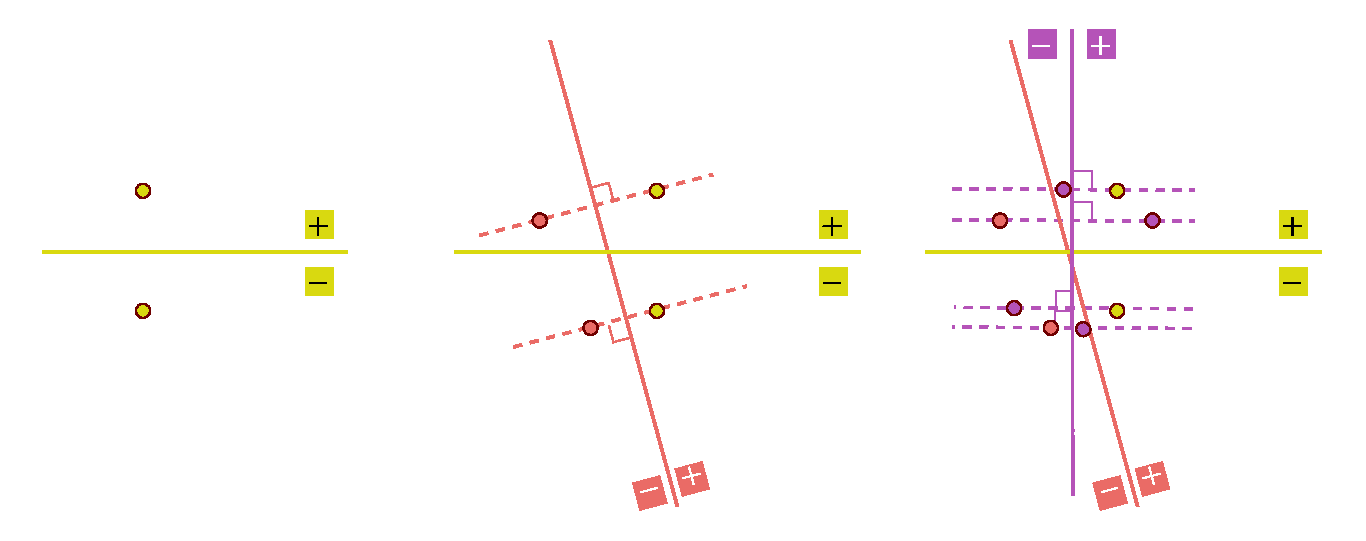
\includegraphics[trim={20 0 20 0},clip,width=1\linewidth]{img/chapter_2/gu_et_al_alg.pdf}
  \caption{Left: Two points are created on either side of the hyperplane. Middle: Another hyperplane is added, and the previously created points are copied to the other side of the new hyperplane. In (\cite{guCounterfactualIdentificationLatent2022}), the authors found a distance computation to ensure that the new points are in the closest region. Right: Repeat with another added hyperplane and remove duplicates, i.e., points with the same sign vector.}
  \label{fig:gu_et_al_algo}
\end{figure}

The two previous cell enumeration methods are interesting, given the correspondence between cells and vertices, but other algorithms exist to convert zonotope generators to a different representation, such as its bounding hyperplanes. However, since the focus here is on enumerating vertices, the conversion between bounding hyperplanes and vertices must be considered. Avis and Fukuda offer such a conversion algorithm in (\cite{avisPivotingAlgorithmConvex}) with a time complexity of $O(n_h n n_v)$, where $n$ is the dimension of $n_h$ hyperplanes, and $n_v$ is the number of vertices created by intersecting them. A method that uses bounding hyperplanes is detailed in the following paragraph.

\paragraph*{Gouttefarde and Krut's hyperplane shifting method (HS) (\cite{gouttefardeCharacterizationParallelManipulator2010a}).}
The number of bounding hyperplanes of a zonotope $\Zono(n,m)$ in general position is $f_{n-1}(\Zono) = 2\binom{m}{n-1}$, i.e., the $(n-1)$-dimensional faces of the $m$-cube project directly onto the zonotope's bounding hyperplanes. Since the position of each $(n-1)$-face in the $m$-cube is known, it remains to project the position and the $(n-1)$-space through the generator matrix and then compute the normal vectors. Using symmetry, the algorithm only needs to enumerate $\binom{m}{n-1}$ hyperplanes. Its time complexity is thus $O(\binom{m}{n-1})$ since all linear operations in the algorithm (computing normals, projecting, etc.) are necessarily bounded by $\binom{m}{n-1}$. This work utilizes the Python implementation package Pycapacity (\cite{skuricPycapacityRealtimeTaskspace2023}).

Table \ref{tab:theoretic_comparison_complexity} presents the time complexity of the three methods described above, compared to EdgeEnum.

\begin{table}[!ht]
    \centering
    \begin{tabular}{|c||c|c|c|c|}
    \hline
    Algorithm & \makecell{Pivot} & \makecell{HS} & \makecell{GRS} & \makecell{EdgeEnum} \\
    \hline
    \hline
    \makecell{Initial enumeration type} & Cell & Hyperplane & Cell & Edge \\ \hline
    \makecell{Time complexity} & $mf_0 \text{lp}(m,n$) & $\binom{m}{n-1}$ & $mf_0\text{mat}(m)$ & $nm^2f_1$ \\ \hline
    \makecell{Additional complexity \\ to convert to vertices} & $nmf_0$ & \makecell{$\binom{m}{n-1}nf_0$} & $nmf_0$ & $nmf_1$ \\ \hline
    \makecell{Total complexity \\ for $n$ fixed} & $m^{n+2.38}$ & $m^{2n-1}$ & $m^{n+1}$ & $m^{n+1}$ \\ \hline
    
    \end{tabular}
    \caption{Time complexity comparison between combinatorially equivalent enumeration algorithms when considering an $n$-dimensional zonotope with $m$ generators in general position. $f_0$ corresponds to its maximal number of vertices, and $f_1$ to its number of edges. Pivot denotes Avis and Fukuda's pivoting algorithm (\cite{avisPivotingAlgorithmConvex}), HS stands for Gouttefarde and Krut's hyperplane shifting method (\cite{gouttefardeCharacterizationParallelManipulator2010a}), and GRS is Gu et al.'s algorithm (\cite{guCounterfactualIdentificationLatent2022}). $\text{lp}(m,n)$ represents the time complexity to solve a linear program of $m$ equations with $n$ variables, and $\text{mat}(m)$ denotes the time cost to determine whether two vectors of length $m$ are identical. In (\cite{cohenSolvingLinearPrograms2020}), the authors created an algorithm that solves a linear program of $m$ equations and $n$ variables with the time complexity of matrix multiplication, approximately $m^{2.38}$. Using a programming language such as R or Python, $\text{mat}(m) = m$. In (\cite{avisPivotingAlgorithmConvex}), the created algorithm converts a set of $n_h$ hyperplanes to $f_0$ vertices with a time complexity of $O(n_h n f_0)$. The total complexity of HS is computed using Stirling's approximation of $\binom{m}{n}$ when $m$ gets large: $\binom{m}{n-1} \approx m^{n-1}/(n-1)! = O(m^{n-1})$ if $n$ is fixed.}
    \label{tab:theoretic_comparison_complexity}
\end{table}

The case of fixed $m$ and large $n$ is not of interest. If the number of generators $m$ is smaller than the dimension of the associated zonotope, enumerating the zonotope vertices necessarily requires enumerating \textbf{all} of the $m$-cube vertices (which amounts to $2^m$). Therefore, no algorithm can be more optimal than a naive algorithm that lists all the $m$-cube vertices.

However, a strong theoretical limitation arises when $m$ and $n$ grow at the same rate. For a preliminary analysis, note that when $n$ has approximately the same growth as $m$, $f_0(\Zono)$ is upper-bounded by $O(2^m)$, and $f_1(\Zono)$ is upper-bounded by $O(m2^{m-1})$ in the worst-case scenario (which occurs when $m=n$).
Thus, in this case, the algorithm with the best time complexity is that of (\cite{guCounterfactualIdentificationLatent2022}) (which grows as $O(m^2 2^m)$), while EdgeEnum lags behind, even preceded by a naive algorithm (of time complexity $O(m2^m)$), with a theoretical time complexity bounded by $O(m^4 2^{m-2})$. 

These results indicate that EdgeEnum theoretically performs similarly to the best state-of-the-art enumeration algorithm (\cite{guCounterfactualIdentificationLatent2022}) when there are many more generators than the ambient dimension of the produced zonotope. This scenario is relevant when considering a large number of muscles to produce the torque feasible set.

\section{Time benchmarks}
\label{time_benchmark}

Theoretical time complexity analysis is insufficient for a complete time study. A time benchmark must be performed on the different algorithms to evaluate the practical relevance of the edge-based vertex enumeration algorithm.
For instance, cell enumeration algorithms such as those in (\cite{radaNewAlgorithmEnumeration2018}) and \cite{guNonparametricMaximumLikelihood2020} have the same asymptotic bounds as in (\cite{avisPivotingAlgorithmConvex}) for hyperplane arrangements in dimensions greater than or equal to $3$, but they appear to exhibit faster computation times in practice (\cite{guCounterfactualIdentificationLatent2022}).

\subsection{Benchmark results}
\label{subsec:benchmark_results}

A computational time benchmark was performed to evaluate the relevance of a zonotope edge-based approach to vertex enumeration for faster computation. A Dell XPS15 laptop computer with a WSL2 and Ubuntu 22.01 operating system was used. This computer is equipped with 11th Gen Intel i9-11950H processors at 2.60GHz. Each core has two threads. The benchmark is implemented in Python 3.10 with the library \emph{numpy} 1.26.4 and default packages such as \emph{itertools} for rapidly generating cube vertices. The \emph{HS}, \emph{GRS}, and \emph{EdgeEnum} algorithms are implemented in Python, whereas \emph{Pivot} is implemented directly in C++ and uses the package \emph{libzonotope} for a Python interface. The edge-based algorithm requires a convex hull computation, which uses \emph{QuickHull}, available in Python through the library \emph{scipy}.


Table \ref{tab:benchmark_time} summarizes the means and standard deviations (in seconds) for each considered algorithm over 10 generator matrices $G\in\IRnm$, with values sampled from a uniform distribution between $-1$ and $1$.

\begin{table}[!ht]
    \centering
    \begin{tabular}{|c|c|c|c|c|}
    \hline
    $(n,m)$ & \makecell{Pivot} & \makecell{HS} & \makecell{GRS} & \makecell{EdgeEnum} \\
    \hline
    \hline

    % $(2, 10)$ & $<0.01$ & $<0.01$ & $<0.01$ & $<0.01$ \\
    % \hline
    $(2, 25)$ & $0.02 \pm 0.00$ & $\mathbf{<0.01}$ & $\mathbf{<0.01}$ & $0.02\pm 0.00$ \\
    \hline
    $(2, 50)$ & $0.08 \pm 0.00$ & $\mathbf{<0.01}$ & $\mathbf{<0.01}$ & $0.09\pm 0.00$ \\
    \hline
    \hline
    
    % $(3, 10)$ & $0.02\pm 0.00$ & $<0.01$ & $0.01\pm 0.00$ & $0.01 \pm 0.00$ \\
    % \hline
    $(3, 25)$ & $0.45\pm 0.01$ & $\mathbf{0.03\pm 0.00}$ & $0.04\pm 0.00$ & $0.14\pm 0.01$ \\
    \hline
    $(3, 50)$ & $4.25\pm 0.05$ & $\mathbf{0.14\pm 0.00}$ & $0.37\pm 0.02$ & $1.44\pm 0.03$ \\
    \hline
    \hline
    
    % $(4, 10)$ & $0.11\pm 0.00$ & $0.02\pm 0.00$ & $0.08\pm 0.01$ & $0.03\pm 0.01$ \\
    % \hline
    $(4, 15)$ & $0.66\pm 0.01$ & $\mathbf{0.08\pm 0.00}$ & $0.09 \pm 0.00$ & $0.14\pm 0.01$ \\
    \hline
    $(4, 20)$ & $2.41\pm 0.07$ & $\mathbf{0.21\pm 0.00}$ & $0.29\pm 0.01$ & $0.48\pm 0.02$ \\
    \hline
    \hline

    % $(5, 10)$ & $0.34\pm 0.02$ & $0.09\pm 0.00$ & $0.30\pm 0.00$ & $0.10\pm 0.00$ \\
    % \hline
    $(5, 15)$ & $3.60\pm 0.08$ & $0.80\pm 0.01$ & $\mathbf{0.42\pm 0.01}$ & $0.97\pm 0.01$ \\
    \hline
    $(5, 20)$ & $17.99\pm 0.14$ & $4.25\pm 0.06$ & $\mathbf{2.80\pm 0.11}$ & $6.55\pm 0.29$ \\
    \hline
    \hline

    $(6, 10)$ & $0.73\pm 0.02$ & $0.58\pm 0.05$ & $\mathbf{0.10\pm 0.00}$ & $0.43\pm 0.01$ \\
    \hline
    $(6, 11)$ & $1.48\pm 0.05$ & $1.39\pm 0.12$ & $\mathbf{0.19\pm 0.01}$ & $0.92\pm 0.01$ \\
    \hline
    $(6, 12)$ & $2.73\pm 0.07$ & $2.86\pm 0.22$ & $\mathbf{0.33\pm 0.02}$ & $1.80\pm 0.05$ \\
    \hline
    \end{tabular}
    \caption{Mean and standard deviation of computation time (in seconds) for $10$ randomly generated zonotopes using different zonotope enumeration algorithms. All generators are in general position, and all algorithms returned the expected number of vertices, $f_0$. The conversion time from a specific representation to vertices is included for each algorithm.}
    \label{tab:benchmark_time}
\end{table}

The hyperplane shifting algorithm (HS) is the fastest in almost all cases for $n\leq 4$, even though it theoretically has the worst time complexity of the presented algorithms. However, as the dimension $n$ increases, its complexity grows combinatorially, which could explain why GRS is the fastest from dimension 5 onward. While EdgeEnum exhibits equivalent time complexity than GRS, the difference observed probably result from the asymptotic growth on the number of $k$-faces  in Lemma \ref{th:big_O_nb_k_faces}: while it states that vertices or edges number has an asymptotic growth in $O(m^{n-1})$, this does not mean that the number of edges is similar to the number of vertices. It is much higher, and is reflected in the time computation benchmark. 

\subsection{Parallelization of EdgeEnum}

To improve the time performance of EdgeEnum, \emph{parallelization} could be employed. This refers to distributing parts of an algorithm across multiple processors. Not all algorithms can be parallelized, but for those that can, computation times can be drastically improved.

In EdgeEnum, one part can be distributed: the inner loop in which the convex hull of each group of edges is computed. The new edges gathered after an iteration of this loop do not influence the gathering of other iterations, making it parallelizable. For instance, using the same computational setup as described previously, Table \ref{tab:parallelism_time_benchmark} summarizes the performance of EdgeEnum using either a single processor or two.

\begin{table}[!ht]
    \centering
    \begin{tabular}{|c|c|c|c|c|}
    \hline
    $(n,m)$ & \makecell{EdgeEnum} & \makecell{EdgeEnum Parallel} \\
    \hline
    \hline
    
    $(6, 10)$ & $0.43\pm 0.01$ & $0.14\pm 0.01$ \\ 
    \hline
    $(6, 11)$ & $0.92\pm 0.01$ & $0.28\pm 0.02$ \\
    \hline
    $(6, 12)$ & $1.80\pm 0.05$ & $0.54\pm 0.03$ \\
    \hline
    \end{tabular}
    \caption{Mean and standard deviation of computation time (in seconds) for $10$ randomly generated generator matrices $G\in\IRnm$ per tuple $(n,m)$. EdgeEnum is parallelized across two processors using the Python package \emph{multiprocessing}.}
    \label{tab:parallelism_time_benchmark}
\end{table}

It is noteworthy that the parallelization only appears to have a non-negligible effect for $n\geq 6$. For lower values of $n$, parallelization results in worse computation times due to the overhead required to copy and transfer data between processors. The parallelized version is not compared with other algorithms here, as they are implemented in a non-parallelized manner.

\subsection{Conclusion on practical time computation}
In conclusion, computing the vertices of a zonotope $\Zono(n,m)$ requires significant computation time, even though the edge-based approach demonstrates time-theoretic efficiency. This is due to the combinatorial explosion in the number of zonotope vertices as the number of generators increases. When modeling force or torque feasible sets using a musculoskeletal model, especially in an optimization context where the goal is to find a set of parameters that reproduce \emph{in silico} and \emph{in vivo} force feasible sets (cf. Chapters \ref{chapter:4} and \ref{chapter:5}), a large number of these sets must be computed. As the number of muscles considered increases, the search space expands, necessitating the evaluation of more solutions. A computation time of $\leq 0.2$ seconds for zonotope vertices leads to hours of optimization when considering a reasonably sufficient number of muscles ($\geq 20$).

Because computation time is a major obstacle, approximations of the vertex set of a zonotope will be explored. Their relevance will be assessed in terms of both computation time and the shape they produce.

\section{Approximation of the vertex set}
\label{sec:approximation_of_vertices_zonotope}
While the methods described previously provide the \emph{exact} vertices of a zonotope, the number of vertices to enumerate is a computational bottleneck for all previously cited algorithm: there are too many to store. This often occurs when the number of generators is large, regardless of the dimension $n$. Thus, it is desirable to reduce computation time through approximations.

Approximating the surface of a zonotope can be done in multiple ways, including bounding boxes or various ellipsoid approximations (\cite{cernyGoffinAlgorithmZonotopes2012}; \cite{gasmannScalableZonotopeEllipsoidConversions2020}; \cite{kousikEllipsotopesCombiningEllipsoids2021}; \cite{henkLownerJohnEllipsoids2012}). However, their main drawback is that they do not necessarily preserve the shape of the zonotope. Generally, the quality of the approximation is related to the computation time.

This work focuses on preserving the shape of a zonotope by approximating its vertex set. This can be achieved in two ways: either by computing a subset of vertices that sufficiently expresses the zonotope shape or by finding points close to each zonotope vertex, up to some tolerance. These two approaches are represented by the following algorithms:

\paragraph*{Stinson et al. randomized vertex enumeration (\cite{stinsonRandomizedAlgorithmEnumerating2016}).}
For a zonotope $\Zono(G)$ with $G\in \IRnm$, this algorithm samples vectors in the zonotope space $\IRn$ using a standard Gaussian distribution in $\IRm$. These vectors are then projected onto $\IRm$ via the map $\mathbf{x}\mapsto \text{sign}(G^T\mathbf{x})$, where $\text{sign}$ assigns $-1$ if its input is negative and $1$ otherwise. The resulting vector in $\IRm$ corresponds to a vertex of the $m$-cube. Stinson et al. showed that a vertex created in this way maps to a zonotope vertex with probability $1$. This approach is inherently fast, as it only requires sampling a chosen number of vectors in $\IRn$. However, a significant caveat arises if the zonotope generators have mutually close angles, as shown in Figure \ref{fig:stinson_fail}. In this case, many randomly chosen vectors may map to the same zonotope vertex and rarely to others. To mitigate this, the sampling size must be increased.

\begin{figure}[!htb]
  \captionsetup{justification=centering}
  \centering
  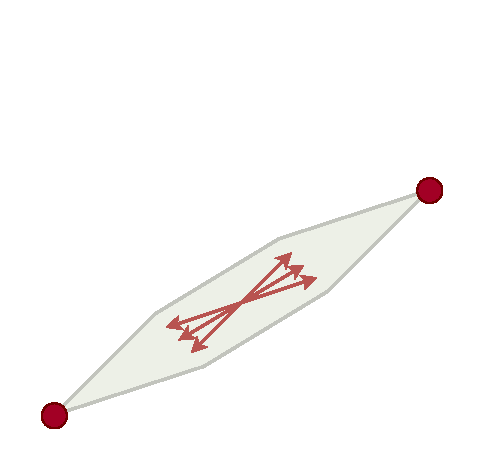
\includegraphics[trim={0 0 0 80},clip, width=0.5\linewidth]{img/chapter_2/stinson_algo_fail.pdf}
  
  \caption{(\cite{stinsonRandomizedAlgorithmEnumerating2016})'s randomized vertex enumeration algorithm. This is an example where the generators have mutually close angles. In this case, the chosen random vectors have a high probability of corresponding to the same zonotope vertex (in red). The sampling size must be increased to avoid this effect.}
  \label{fig:stinson_fail}
\end{figure}

\paragraph*{Skuric et al.'s iterative convex hull method (ICH) (\cite{skuricOnLineFeasibleWrench2022}).}
Recently, a new approximation method for polytope surfaces was proposed in (\cite{skuricOnLineFeasibleWrench2022}). Figure \ref{fig:ich_method} summarizes this method. For a zonotope $\Zono(n,m)$ in $\IRn$, the algorithm begins by selecting $n$ direction vectors in $\IRn$ and then identifies the closest vertices to these directions using a linear program. Iteratively, by selecting new directions based on the normals of the polytope constructed from the convex hull of the found vertices, this algorithm enumerates vertices until a specified tolerance representing how close vertices are from the created directions.
A Python implementation is available and described in (\cite{skuricPycapacityRealtimeTaskspace2023}).

% \begin{figure}[!htb]
%   \captionsetup{justification=centering}
%   \centering
%   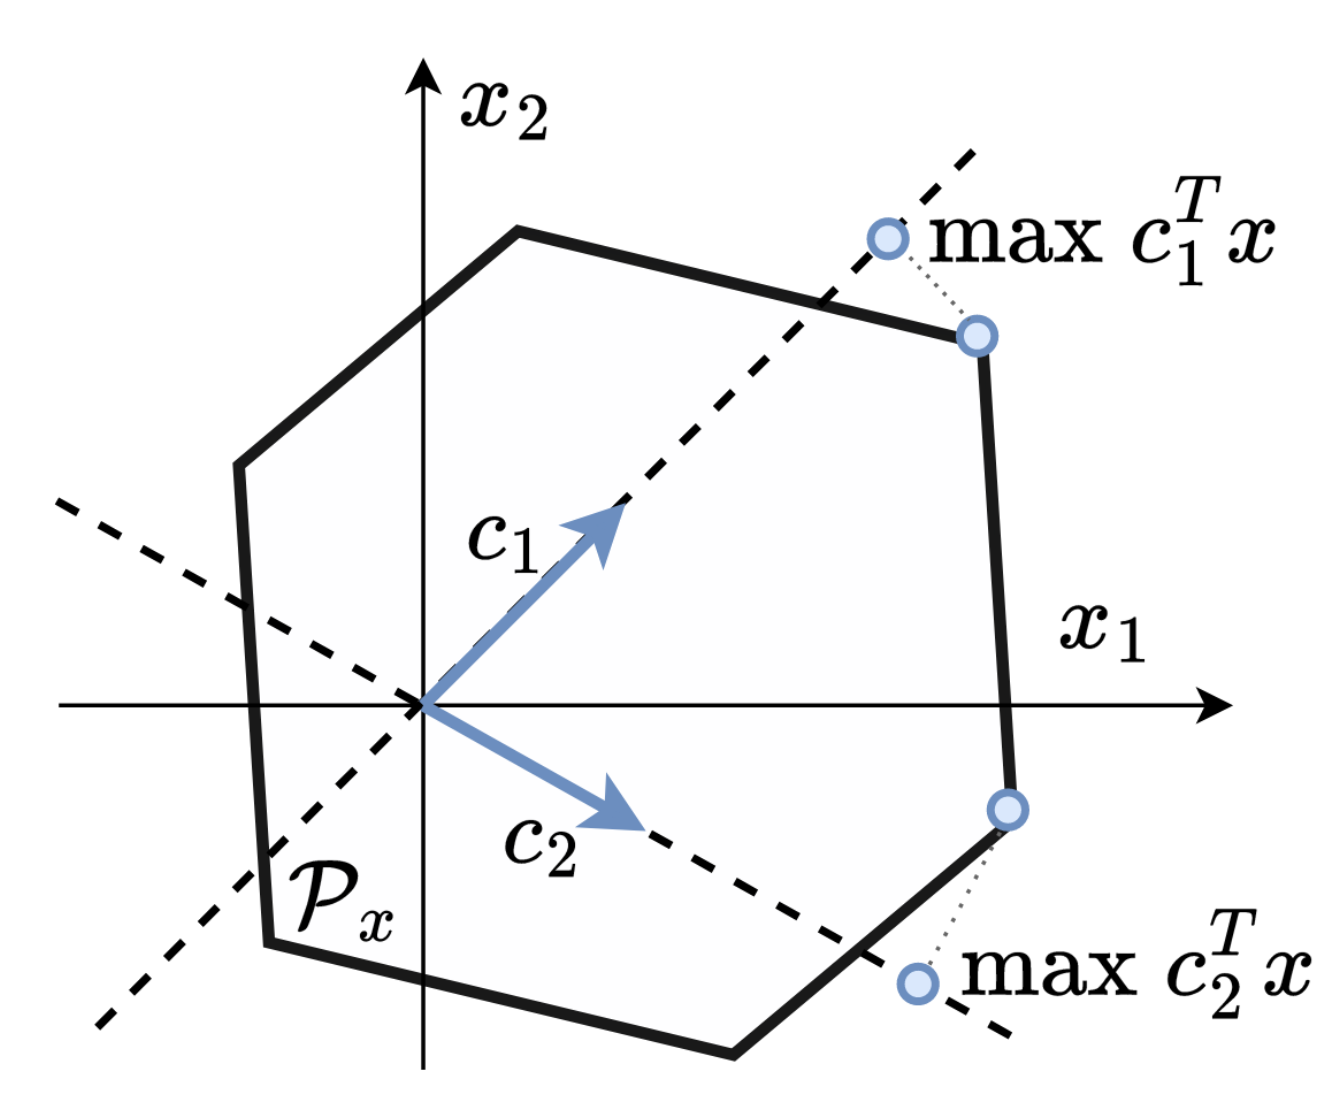
\includegraphics[trim={0 0 0 0},clip, width=0.4\linewidth]{img/chapter_2/ich_alg0.png}
  
%   \caption{Illustration of the Iterative Convex Hull algorithm. Image from (\cite{skuricCoupledViewPhysical}).}
%   \label{fig:ich_method}
% \end{figure}

\begin{figure}[!htb]
    \captionsetup{justification=centering}
    % \begin{minipage}{1\linewidth}
    %     \centering
    %     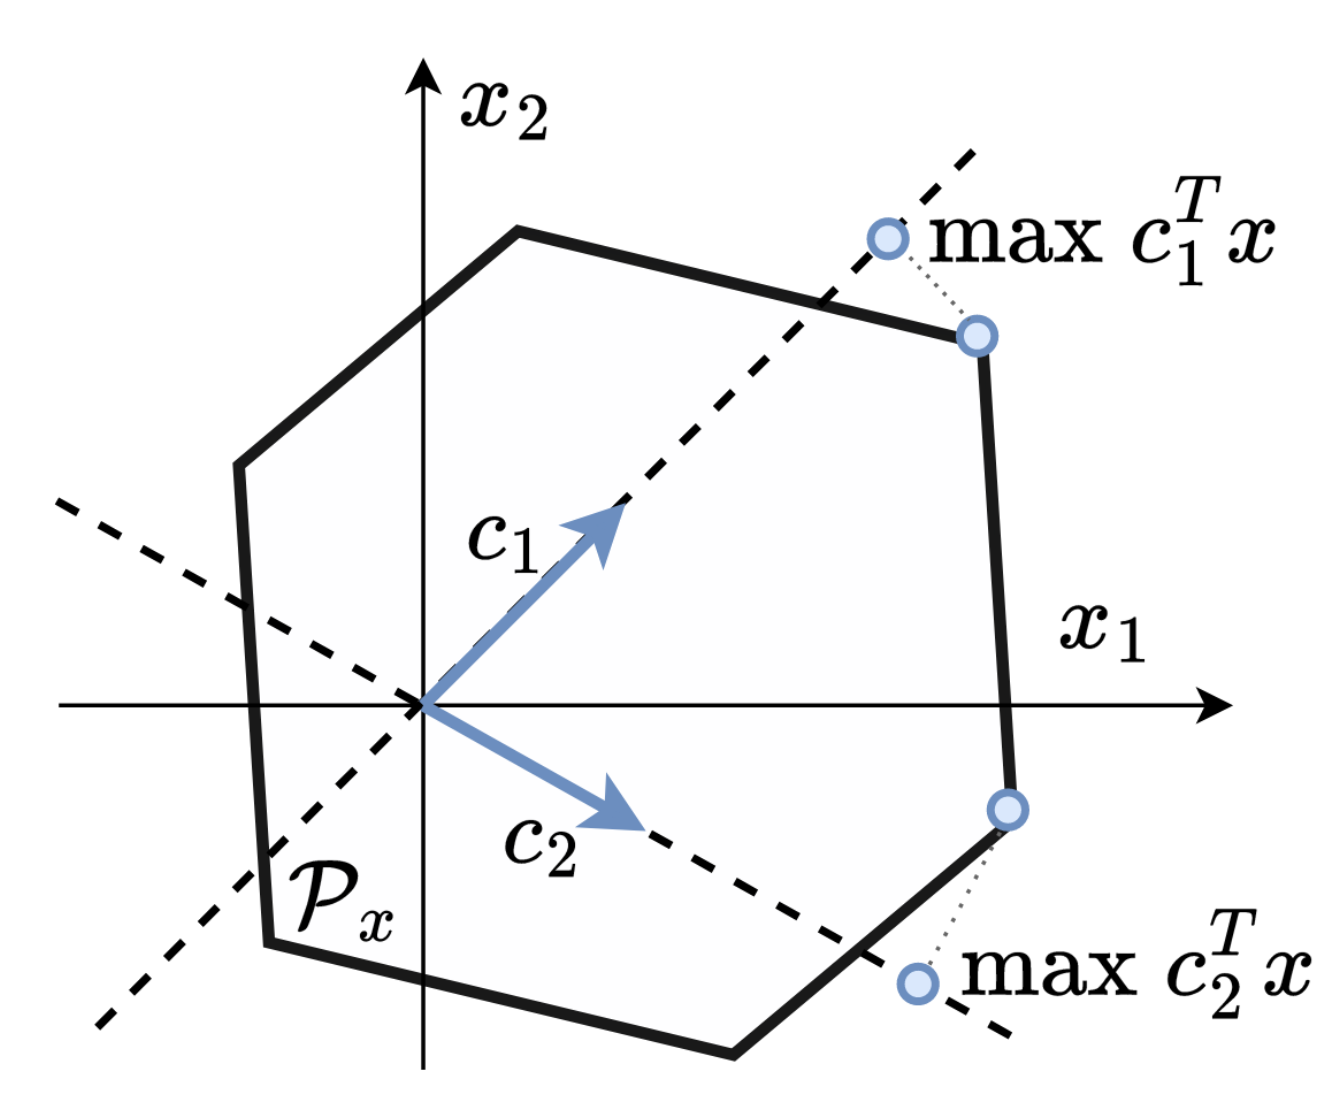
\includegraphics[trim={0 0 0 0},clip, width=0.4\linewidth]{img/chapter_2/ich_alg0.png}
    %     \caption{First step .}
    % \end{minipage}
        \centering
        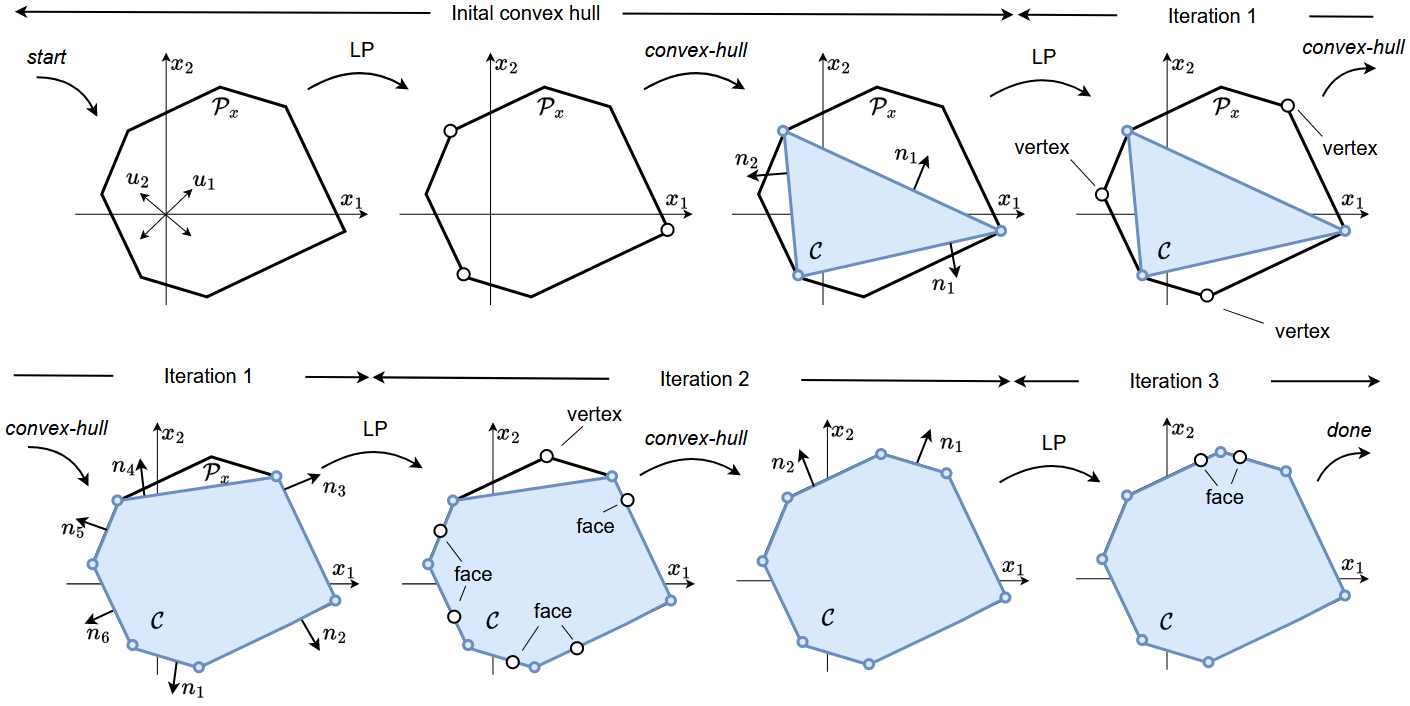
\includegraphics[trim={0 0 0 0},clip, width=1\linewidth]{img/chapter_2/ich_alg.png}
    % \hfill
    % \begin{minipage}{1\linewidth}
    %     \centering
    %     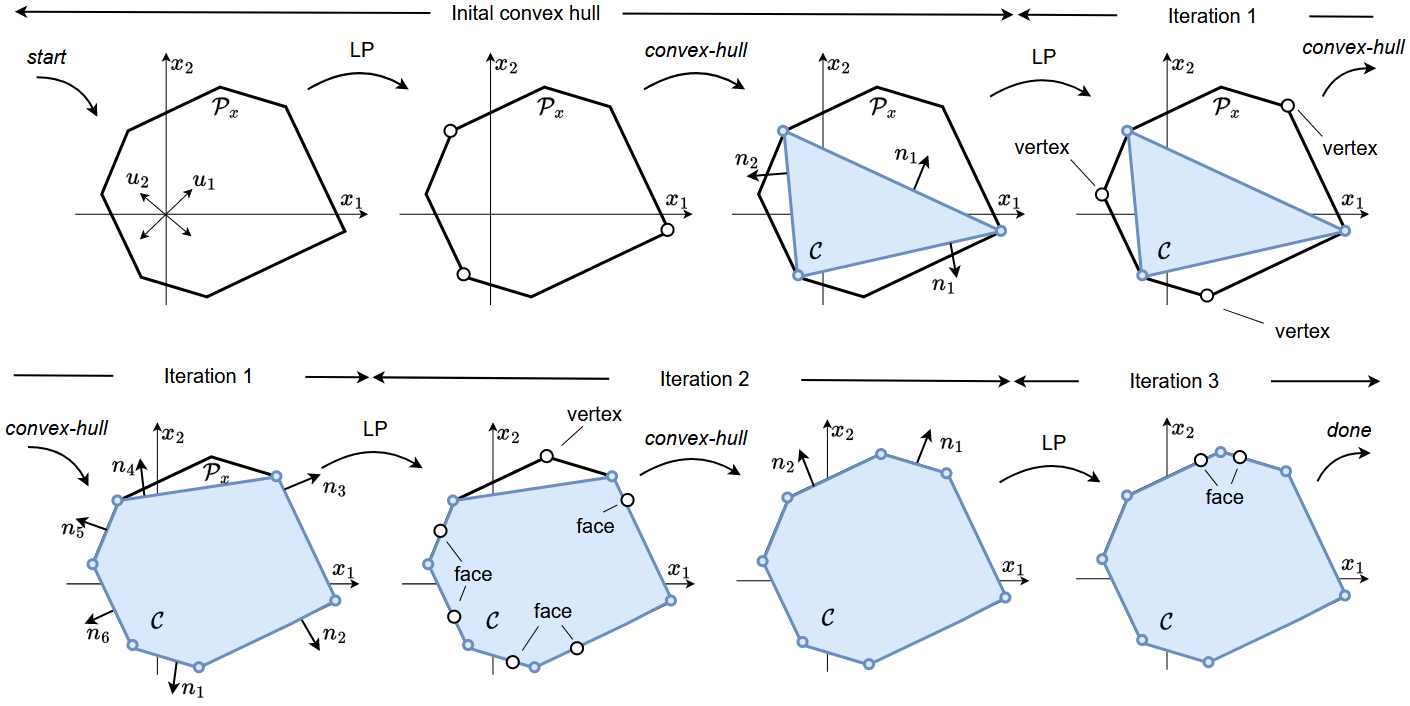
\includegraphics[trim={0 0 0 0},clip, width=1\linewidth]{img/chapter_2/ich_alg.png}
    % \end{minipage}
    \caption{Illustration of the Iterative Convex Hull algorithm. Image from (\cite{skuricCoupledViewPhysical}).}
    \label{fig:ich_method}
\end{figure}

To compare the quality of the vertices produced by each of these algorithms, a suitable metric must be defined. While the Hausdorff distance, a computable distance between sets of points involving the Euclidean distance from every point of one set to every point of another, exists, it is not necessarily a relevant metric in this context. Skuric et al.'s method returns a considerable number of points close to the surface of the zonotope, far exceeding the expected number of vertices. Since the primary interest lies in the global shape of the zonotope, comparing the relative distances of the returned points and the exact vertices would not provide strong information on whether the zonotope's surface is well-approximated. Instead, this work uses the \emph{Jaccard index}, also called the Jaccard similarity coefficient. It is defined for any two sets $A$ and $B$ as
$$J(A, B) = \frac{\text{Vol}(A\cap B)}{\text{Vol}(A\cup B)}$$ where $\text{Vol}$ denotes the volume. 

The Jaccard index, which measures the similarity between two sets, attains a value of 1 when the sets are identical, indicating perfect overlap. For both algorithms presented, the returned points lie \emph{on} the surface of the given zonotope, so the intersection and union are easily computed.

Tables \ref{tab:approx_vertex_set_stinson} and \ref{tab:approx_vertex_set_ich} summarize the computation times for both algorithms for $4$-dimensional zonotopes with $m=15$ or $m=20$ generators, respectively. Table \ref{tab:approx_vertex_set_stinson} shows the results for the randomized enumeration algorithm, and Table \ref{tab:approx_vertex_set_ich} shows the results for ICH algorithm. All computations were performed using the same setup as the previous time benchmark in Subsection \ref{subsec:benchmark_results}.

\begin{table}[!ht]
    \centering
    \begin{tabular}{|c|c|c|c|c|}
    \hline
    $(n,m)$ & \makecell{Number of \\ samples} & \makecell{Computation \\ time} & \makecell{Number found points \\ / exact number of vertices} & \makecell{Jaccard \\ index} \\
    \hline
    \hline

    % $(2, 10)$ & $<0.01$ & $<0.01$ & $<0.01$ & $<0.01$ \\
    % \hline
    \multirow{ 4}{*}{$(4,15)$} & $10$ & $<0.01$ & $0.41\pm 0.03$ & $0.98\pm 0.01$  \\
    \cline{2-5}
     & $100$ & $<0.01$ & $0.67\pm 0.05$ & $\mathbf{1.00\pm 0.00}$  \\
     \cline{2-5}
     & $1000$ & $0.05\pm 0.00$ & $0.83\pm 0.02$ & $\mathbf{1.00\pm 0.00}$ \\
    \cline{2-5}
     & $10000$ & $0.30\pm 0.01$ & $0.93\pm 0.01$ & $\mathbf{1.00\pm 0.00}$ \\
    % \cline{2-4}
    \hline
    \multirow{ 4}{*}{$(4,20)$} & $10$ & $<0.01$ & $0.28\pm 0.01$ & $0.97\pm 0.00$ \\
    \cline{2-5}
     & $100$ & $0.02\pm 0.00$ & $0.56\pm 0.03$ & $\mathbf{1.00\pm 0.00}$ \\
    \cline{2-5}
     & $1000$ & $0.08\pm 0.00$ & $0.78\pm 0.03$ & $\mathbf{1.00\pm 0.00}$ \\
    \cline{2-5}
     & $10000$ & $0.39\pm 0.02$ & $0.89\pm 0.01$ & $\mathbf{1.00\pm 0.00}$ \\
    \hline
    \end{tabular}
    \caption{Performance of (\cite{stinsonRandomizedAlgorithmEnumerating2016})'s randomized algorithm. For each row, $10$ randomly generated $4$-dimensional zonotopes with $m$ generators are computed. The `Number of Samples' column indicates the number of vertices randomly drawn at each iteration. Computation times are in seconds.}
    \label{tab:approx_vertex_set_stinson}
\end{table}

\begin{table}[!ht]
    \centering
    \begin{tabular}{|c|c|c|c|c|}
    \hline
    $(n,m)$ & Tolerance & \makecell{Computation \\ time} & \makecell{Number found points \\ / exact number of vertices} & \makecell{Jaccard \\ index} \\
    \hline
    \hline

    % $(2, 10)$ & $<0.01$ & $<0.01$ & $<0.01$ & $<0.01$ \\
    % \hline
    \multirow{ 4}{*}{$(4,15)$} & $1$ & $0.03\pm 0.01$ & $0.03\pm 0.01$ & $0.56\pm 0.05$  \\
    \cline{2-5}
    & $0.1$ & $0.29\pm 0.02$ & $0.72\pm 0.10$ & $0.98\pm 0.00$ \\
    \cline{2-5}
    & $0.01$ & $0.39\pm 0.01$ & $1.94\pm 0
    .6$ & $\mathbf{1.00\pm 0.00}$\\
    \cline{2-5}
    & $0.001$ & $0.39\pm 0.02$ & $2.12\pm 0.04$ & $\mathbf{1.00\pm 0.00}$ \\
    \hline
    \multirow{ 4}{*}{$(4,20)$}& $1$ & $0.06\pm 0.01$ & $0.03\pm 0.01$ & $0.68\pm 0.05$ \\
    \cline{2-5}
    & $0.1$ & $0.54\pm 0.03$ & $0.61\pm 0.05$ & $0.99\pm 0.00$ \\
    \cline{2-5}
    & $0.01$ & $0.64\pm 0.04$ & $1.36\pm 0.07$ & $\mathbf{1.00\pm 0.00}$ \\
    \cline{2-5}
    & $0.001$ & $0.62\pm 0.04$ & $1.37\pm 0.07$ & $\mathbf{1.00\pm 0.00}$ \\
    \hline
    \end{tabular}
    \caption{Performance of (\cite{skuricOnLineFeasibleWrench2022})'s ICH algorithm. For each row, $10$ randomly generated $4$-dimensional zonotopes with $m$ generators are computed. The "Tolerance" column indicates how close a computed point should be to the zonotope surface. Computation times are in seconds.}
    \label{tab:approx_vertex_set_ich}
\end{table}

These tables confirm that both algorithms can produce a set of points that yield a shape similar to that of a given zonotope. Stinson et al.'s algorithm produces such a set very quickly compared to exact algorithms, with a number of required points much smaller than the exact amount. However, Škuric et al.'s method requires setting a low tolerance to ensure that the points it produces are close to the zonotope surface, leading to longer computation times associated with a larger number of generated points. 

While the results concerning exact and approximation algorithms relate to the surface description of a zonotope, the problems are fundamentally different. This section demonstrated that in the context of describing the shape of the torque feasible set, an exact enumeration algorithm should \textbf{not} be used when considering a large number of muscles. However, working with exact algorithms provided insights into the geometric processes that occur when describing the projection of a tension feasible set modeled as an orthotope. This understanding is key to generalizing the projection process for any convex shape of $\mathcal{T}$, which is the focus of Chapter \ref{chapter:3}.

\section{Conclusion}
\label{conclusion_zonotope_enum_algorithm}
This chapter focused on explicitly computing the torque feasible set 
\begin{align*}
    \left\{\tau \in \IR^n \mid \exists \mathbf{t}\in\mathcal{T}, \quad \tau = -L^T\mathbf{t} - \mathbf{G}\right\}
\end{align*}
assuming that $\mathcal{T}$ is an orthotope, and without loss of generality, an $m$-dimensional cube. The resulting set is a zonotope, which can be described through various representations, including a set of vertices. However, in this case, the torque feasible set is associated with the matrix $-L^T$, which does not directly reveal the global shape of its associated zonotope. 

This chapter proposed an efficient algorithm, called EdgeEnum, to compute the exact vertices of a zonotope based on its edge enumeration. Its time and space complexity were compared theoretically with those of several state-of-the-art zonotope vertex enumeration algorithms, demonstrating that EdgeEnum is a theoretically performant algorithm for worst-case scenarios, i.e., when the number of columns of $-L^T$ is large compared to its number of rows ($n\ll m$).

However, in practice, the algorithm may not be performant due to the unavoidable combinatorial number of edges to enumerate. A time benchmark was performed to highlight this issue. The following paragraphs summarize the benefits and limitations of using an edge-based algorithm.

\subsection*{Strengths of EdgeEnum}

EdgeEnum has several advantages, from its creation process to its implementation.

\paragraph*{Ease of implementation.} EdgeEnum is straightforward to implement. While a recursive version is possible (and implemented in its associated Python package), this chapter presented an implementation based on an iterative construction of the edges of an $m$-cube to emphasize readability and geometric intuition. The only requirement for implementation in any language is the availability of a convex hull operation, which is already natively implemented or available through dedicated libraries in common scientific programming languages such as R, MATLAB, Python, and Julia.

\paragraph*{Parallelism.} A significant advantage of EdgeEnum compared to recent developments is its suitability for parallelization, unlike recent developments such as in (\cite{guCounterfactualIdentificationLatent2022}). This parallelization occurs during the grouping process, in which all current edges during an iteration are separated into groups according to their directions. Applying the convex hull to one group of edges does not require the resulting convex hull of another group. The Python implementation offers both parallel and non-parallel versions of EdgeEnum.

\paragraph*{Theoretical efficiency when $n$ is fixed.} Theorems \ref{th:time_complexity_n_fixed} and \ref{th:space_complexity_n_fixed} showed that the time and space complexity of the algorithm are polynomially bounded in the input and output sizes. This is fundamental, as it qualifies EdgeEnum as an efficient algorithm in terms of both time and space. 

% \paragraph*{Faster than state-of-the-art Algorithms for Large $m$ and $n>6$.} While related to the theoretical notion of efficiency, the numerical time benchmarks show that in practice, EdgeEnum is indeed faster than state-of-the-art algorithms when dealing with a zonotope with a generator matrix in $\IRnm$. Note that for $n=2$, the algorithm can never be better than that of Gu et al. \cite{guCounterfactualIdentificationLatent2022}, as their algorithm reaches near-optimality in this specific case.

\paragraph*{Handling degeneracy.} Degeneracy of a zonotope describes whether its generators are in general position. If they are, the zonotope is not degenerate. The only condition to handle degeneracy is the ability of the convex hull operation to return multiple points that are located at the same position. In this case, the convex hull time complexity is not $O(n\log h)$, where $n$ is the number of points, and $h$ is the number of points on the convex hull. Instead, it is $O(n\log n)$ on average, using an algorithm like \emph{QuickHull} (\cite{barberQuickhullAlgorithmConvex1996}). When applying this new bound to the computed theoretical complexities, the result does not change. However, the computed complexities become \emph{average} bounds, not worst-case bounds. 

The following paragraphs describe several drawbacks of EdgeEnum.

\subsection*{Limits}
This chapter identified three types of limitations related to theoretical algorithmic results, extension of the method to polytopes, and the thesis's goal of understanding the zonotope surface.

\paragraph*{Non-compactness.} An algorithm is \emph{compact} if its space complexity is polynomially bounded by the input size alone (\cite{fukudaZonotopeConstructionMinkowski2004a}).
While the new approach has polynomial time and space complexity for fixed $n$, it requires storing all edges found in each iteration. Therefore, the algorithm does not have the property of \emph{compactness} as its space complexity is not polynomially bounded by the input size alone (\cite{fukudaZonotopeConstructionMinkowski2004a}). The input size is determined by the generator matrix, which has size $nm$. Even for fixed $n$, the space complexity is $O(m^{n+2})$ and is not bounded by any polynomial $(nm)^{\alpha}$, where $\alpha$ is a positive real number. In other words, the algorithm cannot stream edges once they are found, since an edge may be rejected in a subsequent iteration.

As explained in (\cite{ferrezSolvingFixedRank2005a}), the algorithm falls into the category of \emph{incremental} strategies. This means that the edge enumeration problem is solved inductively by maintaining a list of edges at a certain state. The memory requirement is a critical disadvantage of this kind of approach. Thus, the time efficiency of the algorithm is counteracted by its space requirements.

\paragraph*{Approximation algorithms are better suited for fast zonotope surface description.} 
Even though EdgeEnum remains relevant for some practical problems (\cite{guCounterfactualIdentificationLatent2022}; \cite{fukudaZonotopeConstructionMinkowski2004a}; \cite{guibasZonotopesBoundingVolumes}), it may not be the most suitable choice for describing a zonotope surface. Approximation algorithms can achieve compelling results with significantly faster computation times by identifying a limited number of points on the surface. The convex hull of these points closely approximates the desired zonotope (in terms of volume), as demonstrated in Section \ref{sec:approximation_of_vertices_zonotope}.

Consequently, for the remainder of this thesis, all vertex computations of force feasible sets represented as polytopes will employ an approximation approach. Since Chapter \ref{chapter:4} involves computing a large number of force polytopes to determine the parameters of a musculoskeletal model from \emph{in silico} force polytopes, the Iterative Convex Hull method (\cite{skuricOnLineFeasibleWrench2022}) will be used for all polytope computations. The chosen tolerance will vary depending on the context.

\paragraph*{EdgeEnum does not (always) extend to the vertex enumeration of zonotope sections.} While this chapter presented results concerning the torque feasible set, our thesis focuses on force feasible sets, including those modeled as polytope, i.e., a section of a zonotope. If $p$, the dimension of this section, equals $n-1$, then it is possible to construct some vertices of the polytope resulting from this section (cf. Figure \ref{fig:zonotope_section_2D_example}). If the affine subspace sectioning the zonotope is in general position (i.e., it does not cross any vertices of the zonotope), then it is even possible to enumerate all of its vertices. However, in this context, the force feasible set is usually described in 3D, the torque space in 7D, and the tension space in $mD$ for $m\geq 7$, so it is not possible to return all vertices. This is mainly because the polytope vertices are produced by intersecting this affine space with higher-dimensional faces of the zonotope, not necessarily \emph{only} with edges.

\begin{figure}[!htb]
  \captionsetup{justification=centering}
  \centering
  \includegraphics[trim={0 0 0 0},clip, width=0.4\linewidth]{img/chapter_2/polytope_section_zono.pdf}
  \caption{An affine subspace $L$ of dimension $1$ that does not intersect any zonotope vertices is shown in yellow. In this case, because $1 = n-1$, where $n=2$ is the dimension of the zonotope, it is possible to construct the vertices of this zonotope section by intersecting $L$ with the edges it crosses.}
  \label{fig:zonotope_section_2D_example}
\end{figure}

\subsection*{On the cubical representation of the tension feasible set}
The novel algorithm presented in this chapter is theoretically relevant to the vertex enumeration subfield of computational geometry. It sheds new light on enumeration techniques. To the best of our knowledge, most enumeration algorithms consider cube vertices, hyperplanes, and sign vectors, but rarely edges. This may be because the number of cube edges is much larger than the number of cube vertices.

In practice, the number of zonotope vertices grows combinatorially with its number of generators, making \emph{any} enumeration algorithm inefficient with regard to computation time. Section \ref{sec:approximation_of_vertices_zonotope} considered approximations of the zonotope surface to further decrease computation time and reduce the number of points required to describe the zonotope surface. These approximations are relevant in the context of this thesis. 

To reconstruct a musculoskeletal model whose torque feasible sets fit given maximal torque capacities in various postures, it must be possible to generate \emph{in silico} a large number of torque feasible sets and compare them.

However, whether approximations or exact algorithms are used, it was hypothesized that the tension feasible set is shaped as a cube. Biomechanically, this means that all muscles can produce their maximum tensions simultaneously. The next chapter will consider other shapes and their associated biomechanical assumptions to focus on their produced force feasible set shape. The creation process of EdgeEnum is a first step in this direction. This chapter described the global shape of the torque feasible set by navigating between the tension feasible set and its projection onto the torque space. More generally, the shape of the tension feasible set and its projection (followed or not by an intersection) are strongly linked. They are even \emph{inextricable}, and the main results of the next chapter argue that the shape of the tension feasible set does not strictly matter when a large number of muscles is considered. Surprisingly, these results will lead to a new characterization of force feasible sets and a deeper understanding of muscle tension interactions.

\chapter{A unified model of the tension feasible set}
\label{chapter:3}

\usection{Introduction}
The force feasible set $\mathcal{F}$ can be modeled in various ways depending on the context. Some common representations utilize either an ellipsoid or a polytope (\cite{skuricOnLineFeasibleWrench2022}; \cite{rezzougUpperLimbIsometricForce2021b}; \cite{hernandezImprovingUpperlimbForce2017a}; \cite{bosscherWrenchfeasibleWorkspaceGeneration2006a}). Of particular interest is Chiacchio's force manipulability ellipsoid (\cite{chiacchioForcePolytopeForce1997}), which, for a serial kinematic chain with $n$ degrees-of-freedom, is defined as:
\begin{align*}
\mathcal{F}_{\text{Chiacchio}} := \{\mathbf{f}\in\mathbb{R}^3 \mid J^T\mathbf{f} = \tau,\quad \tau^T\tau\leq 1\}
\end{align*}
where $J^T$ is the transpose of the Jacobian matrix $J\in\mathbb{R}^{3\times n}$ expressed at the end-effector, and $\tau\in \mathbb{R}^n$ represents the feasible torques.  Chiacchio's model assumes that the torque feasible set is bounded by a sphere of radius 1 ($\tau^T\tau \leq 1 \iff \|\tau \|_2 \leq 1$).  Geometrically, this can be visualized as the intersection of a unit sphere in $\mathbb{R}^n$ with $\im J^T$, the vector space spanned by the columns of $J^T$, resulting in a force ellipsoid. To express this ellipsoid in the Cartesian force space, the Moore-Penrose pseudo-inverse of $J^T$, denoted by $(J^T)^+$, is applied on it. This is valid because the pseudo-inverse acts as the classic inverse for elements within $\im J^T$, effectively mapping points from the intersection in the torque space back to their corresponding force vectors in $\mathbb{R}^3$.
\begin{figure}[!htb]
 \captionsetup{justification=centering}
  \centering
  \includegraphics[trim={80 20 50 120}, clip, width=0.5\linewidth]{img/chapter_3/chiacchioellipsoid.png}
 \caption{Chiacchio's force ellipsoid expressed in the torque space (in red) (\cite{chiacchioForcePolytopeForce1997}). The feasible torques (in blue) are modeled as a ball of radius 1. The intersection with $\im J^T$ (green plane) produces a lower-dimensional ellipsoid (in red) defining Chiacchio's force ellipsoid expressed in the torque space.}
 \label{fig:chiacchio_ellispoid}
\end{figure}

While providing a useful framework, Chiacchio's construction does not explicitly incorporate muscle considerations. However, such considerations can be integrated by adjusting the radius of the torque feasible sphere to align with experimental data, as done in (\cite{rezzougUpperLimbIsometricForce2021b}). This raises the question of whether this scaling process adequately captures the complex interplay between muscles and joint torques. To address this, we adopt a more comprehensive approach by considering all possible models for the force feasible set, aiming to derive general results applicable to any model choice.

In this broader context, the isometric force feasible set, $\mathcal{F}$, for a $p$-dimensional kinematic chain with $n$ degrees-of-freedom and $m$ muscles (where $p \leq n \leq m$) at a specific posture is defined as:
\begin{align*}
 \mathcal{F} = \left\{ \mathbf{f}\in\mathbb{R}^p \mid \exists \mathbf{t}\in \mathcal{T},\quad J^T\mathbf{f} = -L^T\mathbf{t} - \mathbf{G}\right\}
\end{align*}
where $J^T\in\mathbb{R}^{n \times p}$ is the transpose of the Jacobian matrix (mapping end-effector forces to joint torques), $L\in\mathbb{R}^{m \times n}$ is the lever-arm matrix (where $-L^T$ maps muscle tensions to joint torques), $\mathbf{G}\in\mathbb{R}^n$ is the gravitational torque vector, and $\mathcal{T}\subset \mathbb{R}^m$ is the set of possible muscle tension combinations.

It is easily seen that Chiacchio's ellipsoid, in its raw form, corresponds to the case in which: gravity is not considered; the tension feasible set $\mathcal{T}$ is a centered sphere in $\mathbb{R}^m$ of radius 1; and $-L^T$ is an orthogonal projection from the tension space to the torque space. In other words, there are many simplifying assumptions regarding how muscles act on joints. The general force feasible set formulation require the following assumptions: 1) the muscle geometry must be known to compute the lever arms in $-L^T$; 2) the minimal and maximal tensions of each muscle must be known to estimate the possible values taken by $\mathbf{t}$; and 3) the neuromuscular behavior should be understood to properly model the shape of $\mathcal{T}$. 

Indeed, in this framework, the tension feasible set can be viewed as a linear transformation of the set of all possible muscle activations. Since muscles may be activated according to the activation of neighbor muscles (a behavior termed \emph{muscular grouping}), or activated according to an agonistic-antagonistic relationship with another muscle, this is equivalent to assuming a pairwise relationship between muscles. Consequently, the global shape of the tension feasible set is determined by a linear transformation of the activation set.  

Figure \ref{fig:formula_} illustrates this construction geometrically.
\begin{figure}[!ht]
  \centering
  \captionsetup{justification=centering}
  \begin{tikzcd}
    \mathcal{F}' \subset \mathbb{R}^p & \mathcal{F} \subset \mathbb{R}^n \arrow[l] \arrow[l, "(J^T)^+"] & \mathcal{T}_o\subset \mathbb{R}^n \arrow[l, "\cap \im J^T"] & \mathcal{T}\subset \mathbb{R}^m \arrow[l, "-L^T - \mathbf{G}"]
  \end{tikzcd}
  \caption{Description of the geometric operations to derive the force feasible set in isometric conditions. The set of muscle tensions $\mathcal{T}$ is projected and translated onto the torque space to create the torque feasible set $\mathcal{T}_o$. It is then intersected with a vector space ($\im J^T$) to produce the force feasible set $\mathcal{F}$ described in the torque space, or conveniently in the Cartesian force space using $(J^T)^+$. In practice, we prefer to express $\mathcal{F}$ in the torque space since $(J^T)^+$ is a bijection between $\mathcal{F}$ and $\mathcal{F}'$.}
  \label{fig:formula_}
\end{figure}

A straightforward application of this general formula arises when all muscles are considered fully activable simultaneously. In this scenario, the tension feasible set $\mathcal{T}$ is a linear transformation of a cube, resulting in an \emph{orthotope} (or hyperrectangle). This orthotope is then projected onto the torque space, producing a zonotope that represents all feasible torques. Consequently, the force feasible set, formed by the intersection of this zonotope with $\im J^T$, is a polytope.  We refer to this model, with the orthotopic assumption on the tension feasible set, as the $\mathcal{T}_{\infty}$ model.  Alternatively, if $\mathcal{T}$ is a linear transformation of a sphere (resulting in an ellipsoid), we call it a $\mathcal{T}_2$ model. In this chapter, we will consider a broader class of possible models, denoted $\mathcal{T}_p$, for $2 \leq p < +\infty$. Figure \ref{fig:tension_models} illustrates these two first models.
\begin{figure}[!htb]
  \centering
  \captionsetup{justification=centering}
  \begin{minipage}{0.49\linewidth}
    \centering
    \includegraphics[trim={50 150 50 70}, clip, width=1\linewidth]{img/chapter_3/polytope_better_ggb.png}
  \end{minipage}
  \hfill
  \begin{minipage}{0.49\linewidth}
    \captionsetup{justification=centering}
    \centering
    \includegraphics[trim={50 150 50 70}, clip, width=1\linewidth]{img/chapter_3/polytope_from_sphere_ggb.png}
  \end{minipage}
  \caption{Differences in the shape of the force feasible set $\mathcal{F}$ (in red) based on the modeling choice for the tension feasible set $\mathcal{T}$ (in pink). A $\mathcal{T}_{\infty}$ model implies that $\mathcal{T}$ is a linear transformation of a cube (an orthotope), while a $\mathcal{T}_2$ model is the linear transformation of a sphere (an ellipsoid). The force feasible set $\mathcal{F}$ can be constructed in two steps: first, $\mathcal{T}$ (pink) is projected onto the torque space (light blue plane), forming the torque feasible set $\mathcal{T}_o$ (dark blue). Then, $\mathcal{T}_o$ is intersected with a subspace (green line). All elements in this intersection constitute the force feasible set $\mathcal{F}$ described in the torque space.}
  \label{fig:tension_models}
\end{figure}

However, experimental measurements of maximal force exertions at the hand suggest that a scaled Chiacchio's ellipsoid ($\mathcal{T}_2$ model) underestimates these measurements, while the polytope ($\mathcal{T}_{\infty}$ model) overestimates them (\cite{rezzougUpperLimbIsometricForce2021b}). These estimations, based on in silico force feasible sets, required scaling a generic upper limb musculoskeletal model.
\begin{figure}[!htb]
  \captionsetup{justification=centering}
    \centering
    \includegraphics[trim={0 0 0 0}, clip, width=0.5\linewidth]{img/chapter_3/FFSComparisonRezzoug.png}
  \caption{Two modeled scaled force feasible set boundaries compared to experimental data, expressed in the sagittal plane relative to the upper-limb posture of one participant. The solid line represents the convex hull of experimentally measured maximal force exertions. The black squares depict the in silico force feasible set modeled as a polytope ($\mathcal{T}_{\infty}$ model), while the wire-frame represents the ellipsoid version ($\mathcal{T}_2$ model). The gray circle has a radius of 300N. Image extracted from (\cite{rezzougUpperLimbIsometricForce2021b}).}
  \label{fig:rezzoug_exp}
\end{figure}

Consequently, neither an ellipsoid nor a polytope representation of the force feasible set appears to fully capture the size of measured experimental force exertions. However, they seem to approximate the global orientation of the measured data. Since Chiacchio's ellipsoid does not require knowledge of muscle lever arms, it can be inferred that the Jacobian matrix, $J^T$, plays a crucial role in determining this orientation.

In the aforementioned representations of $\mathcal{F}$, the specific models share one common characteristic: $\mathcal{T}$ is assumed to be convex and symmetric. Most results in this chapter assume symmetry of the tension feasible set, $\mathcal{T}$, which might not always be realistic in a biomechanical context. They are valid for a broad class of nested symmetric shapes, which allows us to consequently extend the results to non-symmetric convex models that can be enclosed in between two arbitrarily chosen symmetric $\mathcal{T}$ shape models. This ensures applicability to a wide range of muscle activation patterns, even those that exhibit some degree of asymmetry. While a spherical shape offers computational advantages, it underestimates the true size of the force feasible set. Conversely, a cubical shape leads to combinatorial challenges, overestimates the size, and introduces unrealistically sharp edges in the context of human biomechanics.

This chapter aims to address these limitations through a deeper understanding of the mathematical formulation of force feasible sets. Our objectives are threefold:
\begin{enumerate}[noitemsep]
  \item \textbf{Decouple size and shape:}  Separate the notions of \emph{size} and \emph{shape} in $\mathcal{F}$ to gain finer control when fitting in silico models to experimental data (cf. Chapter \ref{chapter:5}). We will demonstrate that $\mathcal{F}$ inherently possesses an ellipsoidal shape, regardless of the chosen model, and that this approximation improves with the number of muscles considered.  Furthermore, we will show that the size of $\mathcal{F}$ depends on a coupling between the mean value of maximal muscle tensions and muscle path geometry.
  \item \textbf{Quantify the impact of muscle path geometry:} Analyze how muscle path geometry influences $\mathcal{F}$, and apply this analysis to determine whether personalization of muscle geometry in a scaled generic musculoskeletal model is necessary.
  \item \textbf{Provide modeling guidelines:} Offer insights into how force feasible sets should be modeled depending on the specific context.
\end{enumerate}

To achieve these goals, we seek the most suitable force feasible set model with size and shape consistent with experimental maximal force measurements in isometric conditions. Since these properties depend on the model chosen for the tension feasible set, we consider the class of all convex, symmetric sets for $\mathcal{T}$. This analysis utilizes the theory of Banach spaces (Section \ref{sec:theory_banach_spaces}), which provides a framework for treating symmetric convex sets as vector spaces equipped with a notion of size.

Section \ref{sec:ellipsoidal_shape_ffs} delves into the \emph{Local Theory of Banach spaces} to demonstrate that, irrespective of the choice of model for $\mathcal{T}$, the force feasible set tends to resemble an ellipsoid with high probability. This probability approaches 1 as the number of considered muscles increases, highlighting the role of the geometric construction of $\mathcal{F}$. This section concludes with a computationally amenable reformulation of the general description of $\mathcal{F}$ directly in the tension space, facilitating the analysis of how muscle tension combinations contribute to the force feasible set. While the ellipsoidal approximation is theoretically sound, its computation remains challenging and model-dependent. To overcome this, Section \ref{sec:projected_volume_problem} explores the projection constant theory within the Banach space framework. We show that the problem of fitting the size of $\mathcal{F}$ is directly linked to the choice of model for $\mathcal{T}$ and we propose an explicit computation for an adapted ellipsoid.

Building on the theoretical tools developed in the preceding sections, Section \ref{sec:sensitivity} introduces a novel index quantifying the influence of muscle path geometry (locations of path points and via points) on the force feasible set. This index, independent of the specific model chosen for $\mathcal{T}$, provides valuable insights into whether detailed personalization of muscle geometries is required when scaling a generic musculoskeletal model.

This chapter concludes by summarizing the theoretical analysis of the force feasible set, laying the foundation for the applications explored in the next two chapters, which focus on musculoskeletal model muscle personalization based on the knowledge of \emph{in silico} and \emph{in vivoe} force feasible sets in different postures.

\section{The theory of Banach spaces}
\label{sec:theory_banach_spaces}
This thesis adopts a set-theoretic approach to model the forces exertable by an individual. While intuitive for defining these sets, this approach may seem less practical when comparing force feasible sets between individuals or analyzing the influence of muscle tensions and geometry. To gain a more comprehensive understanding, we shift our perspective while retaining the underlying set-based vision. This section introduces the fundamentals of \emph{Banach spaces}, providing a structured framework for studying the geometry of symmetric convex sets and how unit metrics transform. This framework is based on the principle that \emph{in vivo} force feasible sets should reflect, in a structured manner, how muscle tensions interact. The specific structural properties will thus be thoroughly studied in this chapter to gain insights into muscle feasible tensions and their interactions directly from the force feasible sets.

\paragraph*{Banach space.} A \emph{complete normed vector space} is called a Banach space.  Completeness implies that every Cauchy sequence in the space converges to a limit within that space, ensuring no ``gaps'' or ``missing points''.  A normed space is equipped with a notion of \emph{size} for each element $x$, called the \emph{norm of x}, denoted by $\|x\|_X$ (the subscript may be omitted when the context is clear). Formally, a Banach space is often denoted as $(X,\, \|\cdot \|_X)$. This thesis focuses on \emph{finite-dimensional real-valued normed} vector spaces, where vectors have a finite number of real-valued components.  Such spaces are inherently complete and thus qualify as Banach spaces.

We present two complementary perspectives on Banach spaces:

\begin{enumerate}
  \item{ \textbf{Geometric perspective:} Visualize a Banach space as a vector space containing a centrally symmetric convex set centered at the origin. This set, often referred to as the \emph{unit ball}, can be a sphere, ellipsoid, zonotope, cube, or any other fully-dimensional, centrally symmetric convex set.  Transformations between Banach spaces not only map the underlying vector space but also ``deform'' the unit ball into another convex set.}
  \item{ \textbf{Metric perspective:}  Interpret a Banach space as a vector space with a well-defined notion of a \emph{unit metric system}. This allows us to study how a unit of measurement transforms under different mappings.}
\end{enumerate}

These two perspectives allow us to draw a parallel between the geometric properties of the force feasible set and its physical interpretation. The choice of perspective depends on the context. For instance, we will demonstrate that force feasible sets tend to resemble ellipsoids when a large number of muscles are involved. This result is established by analyzing how the Newton unit, used to quantify muscle tension combinations, undergoes a quadratic transformation to become the Newton-meter unit in the torque space.

While this thesis assumes a familiarity with linear algebra, the geometric and metric perspectives on Banach spaces may be less familiar, particularly in higher dimensions. For an intuitive understanding, we encourage the reader to primarily adopt the geometric viewpoint for now. The following paragraphs introduce fundamental concepts that form the basis of any study on Banach spaces.

\paragraph*{The $p$-norms and $\ell_p^n$ spaces.} Norms provide tools for measuring the \emph{size} of elements in a vector space. In $\mathbb{R}^n$, a common norm is the Euclidean norm (or 2-norm), defined as $\|\mathbf{x}\|_2 = \sqrt{x_1^2 + \dots + x_n^2}$. When $\mathbb{R}^n$ is equipped with $\|\cdot \|_2$, we refer to it as $n$-dimensional Euclidean space. However, other norms can be defined on $\mathbb{R}^n$.  The $p$-norm, denoted by $\|\cdot \|_p$, is given by:
\begin{align*}
\|\mathbf{x}\|_p = \left(\sum_{i=1}^n \vert x_i \vert^{p}\right)^{1/p}
\end{align*}

The Euclidean norm is a special case of the $p$-norm with $p=2$.  Another useful norm is the $\infty$-norm, defined as:
\begin{align*}
\|\mathbf{x}\|_{\infty} = \lim_{p\to \infty} \|\mathbf{x}\|_p = \max_{i=1,\dots,n}\vert x_i\vert
\end{align*}

Each $p$-norm provides an analytical description of the geometry of a specific type of centrally symmetric convex set.  The surface of such a set can be represented as $\{\mathbf{x}\in \mathbb{R}^n \mid \|\mathbf{x}\|_p = 1\}$.  This analytical representation is valuable for our purpose of analyzing and fitting the shapes of force and torque feasible sets.

To clearly indicate which $p$-norm is being used, we adopt the notation $\ell_p^n$ to represent the $n$-dimensional real vector space $\mathbb{R}^n$ equipped with the $p$-norm $\|\cdot \|_p$.

\paragraph*{Unit balls.} A norm quantifies the elongation of a vector relative to a reference value that depends on its direction and the dimension of the ambient space. Similarly, the amplitude of a maximal isometric force exerted at the hand depends on the direction of force application. Choosing a norm for a Banach space $X$ effectively defines how different directions in $X$ influence the elongation of a vector. To capture all possible influences (since there are infinitely many directions for $n \geq 2$), we consider the set $\mathcal{B}_X = \{\mathbf{x}\in X \mid \|\mathbf{x}\|_X \leq 1 \}$, called the \emph{unit ball} of $X$.  For $\ell_p^n$ spaces, we denote their unit balls by $\mathcal{B}_p^n$, as illustrated in Figure \ref{fig:pnorms} for $\ell_p^2$ spaces with various values of $p$.

\begin{figure}[!htb]
  \captionsetup{justification=centering}
    \centering
    \includegraphics[trim={0 0 0 0}, clip, width=0.4\linewidth]{img/chapter_3/p_norms.png}
  \caption{Unit balls associated with different $p$-norms in $\mathbb{R}^2$ (from Wikipedia).}
  \label{fig:pnorms}
\end{figure}

% \paragraph*{Symmetric convex sets and $p$-unit balls.}
% In figure \ref{fig:pnorms}, we can see that the most convenient $p$-norm to work with is $p=2$, the euclidean norm: the notion of size in the considered space is the same in any direction (all directions matter). If we consider $p=\infty$, then we are saying that only the principal direction of a vector matters (\emph{i.e.} its largest component in absolute value). Generalizing these interpretations for $2< p <\infty$, the more large $p$ gets, the more importance is given to the principal direction of a vector. A contrario, the more close to $2$ $p$ gets, the less distinction we make between important directions. This is geometrically represented by \emph{how rounded} the unit ball $\mathcal{B}_p^n$ is, with $\mathcal{B}_2^n$ being a purely rounded ball of radius 1 in $\IRn$ and $\mathcal{B}_{\infty}^n$ being a $n$-dimensional cube centered at origin whose edges are of length $2$. Unit balls $\mathcal{B}_p^n$ are necessarily symmetric around the origin of $\IRn$.

% The point of view we are giving to the reader is thus the following: studying $p$-norms of $\IRn$ corresponds to studying the symmetric convex set associated to their unit balls. This is interesting in theory, but there is not much we can do with this.

\paragraph*{Operators.} Let $X$ and $Y$ be Banach spaces with norms $\|\cdot\|_X$ and $\|\cdot\|_Y$ respectively. An \emph{operator} $T: X \rightarrow Y$ is a continuous linear map between $X$ and $Y$. Operators transform Banach spaces into Banach spaces. Linearity ensures that a vector space is mapped to a vector space, while continuity preserves completeness, guaranteeing that the resulting space after the transformation remains ``whole'' with no ``gaps'' or ``missing points''.

In finite dimensions, any operator $T: X \rightarrow Y$ can be represented by a matrix. However, this matrix representation only captures how the vector space structure of $X$ is transformed under $T$. We need a more comprehensive tool to study how the norm of $X$ is affected by $T$. Since the norm structure of $X$ is characterized by its unit ball, the key question becomes: \emph{How is the unit ball of $X$ transformed by $T$?}

To answer this, we need to consider the properties of $T$. An operator $T: X \rightarrow Y$ is \emph{bounded} if $T(\mathbf{x})$ is bounded for all $\mathbf{x} \in \mathcal{B}_X$.  Since a linear map between normed spaces is continuous if and only if it is bounded, $T$ must be bounded. This implies that the set of operators from $X$ to $Y$ forms a Banach space, which can be equipped with a norm called the \emph{operator norm}, defined as:
\begin{align*}
\|T\|_{op} = \sup\left\{\|T(\mathbf{x})\|_Y \mid \mathbf{x}\in \mathcal{B}_X \right\}
\end{align*}

The operator norm has a clear geometric interpretation: it represents the largest distance between the transformed unit ball of $X$,  $\{T(\mathbf{x}) \mid \mathbf{x}\in \mathcal{B}_X\}$, and the unit ball of $Y$, as depicted in Figure \ref{fig:operator_norm}.
\begin{figure}[!htb]
  \captionsetup{justification=centering}
    \centering
    \includegraphics[trim={150 0 70 0},clip, width=1\linewidth]{img/chapter_3/operator_norm.pdf}
  \caption{Geometric interpretation of the operator norm. $T$ projects $\ell_{\infty}^3$ onto $\ell_2^2$. Its operator norm, $\|T\|_{op}$, is the maximal Euclidean norm of the vectors describing the surface of the projected unit ball of $\ell_{\infty}^3$. In this case, this corresponds to the surface of a zonotope (blue). This is equivalent to computing the maximal 2-norm of the zonotope vertices.}
  \label{fig:operator_norm}
\end{figure}

In essence, the operator norm quantifies the maximal deformation of the transformed unit ball of $X$ relative to the unit ball of $Y$. With this understanding, we are now equipped to delve into the comparison of centrally symmetric convex sets.

\paragraph*{Banach-Mazur distance.} Consider two isomorphic Banach spaces $X$ and $Y$, meaning there exists an invertible linear map between them. Recall that two finite-dimensional real vector spaces are isomorphic if and only if they have the same dimension. In this case, their \emph{Banach-Mazur distance} is defined as:
\begin{align*}
d_{BM}(X,Y) = \inf\{\|T\|_{op} \|T^{-1}\|_{op} \mid T: X\rightarrow Y \text{ is an isomorphism}\}
\end{align*}

If $X$ and $Y$ are not isomorphic, we define $d_{BM}(X,Y) = +\infty$.

When the Banach-Mazur distance is 1, $X$ and $Y$ are said to be \emph{isometric}, meaning they have the same metric structure up to isomorphism. This implies that the set of points at a distance of 1 from the origin in $X$ corresponds exactly to the set of points at a distance of 1 from the origin in $Y$. More generally, as noted in (\cite{milmanDvoretzkyTheoremThirtyYearsLater1992}), for two finite-dimensional real spaces $X$ and $Y$ of the same dimension with respective unit balls $\mathcal{B}_X$ and $\mathcal{B}_Y$, if $d_{BM}(X,Y) \leq d$, then there exists an operator $T: X \rightarrow Y$ such that:
\begin{align*}
\mathcal{B}_X \subset T(\mathcal{B}_Y) \subset d \cdot \mathcal{B}_X
\end{align*}

This means that a linear transformation of the unit ball of $Y$ can be enclosed by the unit ball of $X$ and its dilation by a factor of $d$. Throughout this chapter, we will focus on cases where the unit ball of $X$ is an ellipsoid (so $X = \ell_2^n$), and the unit ball of $Y$ (representing the muscle tension space or the Cartesian force space) is enclosed by an ellipsoid, with $d$ being as close to 1 as possible.

\begin{figure}[!htb]
  \captionsetup{justification=centering}
    \centering
    \includegraphics[trim={0 25 0 25},clip, width=0.5\linewidth]{img/chapter_3/banachmazurdvoretzky.pdf}
  \caption{Building on Figure \ref{fig:operator_norm}, we observe that the projected zonotope lies between a transformation of the disk (an ellipsoid) and a dilation of this ellipsoid by a factor of 1.4. This implies that $d_{BM}(Y, T(X)) \leq 1.4$.}
  \label{fig:banach_mazur_example}
\end{figure}

While the Banach-Mazur distance is a theoretical tool and often cannot be explicitly computed, it will be instrumental in demonstrating strong approximation results in high dimensions in the following sections.

This overview of Banach spaces has introduced mathematical tools for studying centrally symmetric convex sets. This structural approach yields valuable insights, which we will explore in the subsequent sections. With the sole assumption that the tension feasible set is symmetric and convex, we will demonstrate that the \emph{shape} of the force feasible set is largely independent of the specific model chosen for the tension feasible set, while its \emph{size} is model-dependent.

Leveraging the \emph{Local Theory of Banach spaces}, Section \ref{sec:ellipsoidal_shape_ffs} argues that the force feasible set inherently tends to be ellipsoidal due to its geometric construction.  However, in practice, we need to compute this ellipsoidal shape. Section \ref{sec:projected_volume_problem} utilizes the \emph{Projection Constant Theory} to provide a computational tool for approximating the force and torque feasible sets as ellipsoids, taking into account volume changes associated with norm deformations.

% require more depth, in particular results in what it called the \emph{local theory of Banach spaces}, which focuses on studying infinite-dimensional Banach spaces using only finite-dimensional tools. In particular, we are interested in a major result stating that a specific geometric construction over an initial symmetrically convex set will lead to an ellipsoidal shape.

% , section \ref{sec:ellipsoidal_shape_ffs} will show that due to its geometric construction, the force feasible set has a high probability of resembling an ellipsoid. This result is fundamental because it applies \emph{whatever the choice of the tension feasible set shape}. Even better, this ellipsoidal shape \emph{has to} occur due to the small dimensions of the Cartesian force space and the torque space (which is very different from the other perspective on saying that it occurs du to the large amount of muscles). Section \ref{sec:leveraging_the_projected_volume} will dive much deeper in the \emph{projection constant theory}, including a much more theoretical analysis studying problems related to the projection of a physical unit metric onto a subspace. While these sections are underlyingly studying how convex sets are projected and how muscle tensions are deformed onto torques, the final result is a fast explicit computation of the ellipsoidal approximation of the force feasible set.

\section{The ellipsoidal shape of the force feasible set}
\label{sec:ellipsoidal_shape_ffs}
The results in this section are foundational to the \emph{Local Theory of Banach spaces} and provide a valuable theoretical framework. They enable a concise geometric characterization of the force feasible set without imposing specific assumptions on the shape of the tension feasible set $\mathcal{T}$, except for convexity and symmetry. We will leverage the symmetry assumption in certain cases.

We consider various models for the tension feasible set, denoted by $\mathcal{T}_p$, each associated with a linear transformation of a unit $p$-ball. A $\mathcal{T}_2$ model corresponds to a spherical shape, representing a scenario where all muscle activations are equally constrained. In contrast, a $\mathcal{T}_{\infty}$ model assumes a cubic shape, allowing for independent activation of each muscle. The remaining $\mathcal{T}_p$ models, with $2 < p < \infty$, represent intermediate cases with varying degrees of ``roundedness'':
\begin{align*}
\mathcal{T}_2 < \mathcal{T}_3 < \dots < \mathcal{T}_{100} < \dots < \mathcal{T}_{\infty}
\end{align*}

The central result of this section establishes the inherent \emph{ellipsoidal} nature of the force feasible set. This means that $\mathcal{T}_p \approx \mathcal{T}_2$ for any $p \geq 2$, and more generally, $\mathcal{T} \approx \mathcal{T}_2$ for any convex, symmetric tension feasible set. The term ``ellipsoidal'' emphasizes that the force feasible set resembles an ellipsoid globally but may not perfectly coincide with one. However, it can be effectively approximated by an ellipsoid that captures the essential features of its shape. Our goal is to compute this approximating ellipsoid (see Section \ref{sec:projected_volume_problem}), but first, we need to elucidate the underlying reasons for this phenomenon and the conditions under which such an approximation is valid.

Before delving into the mathematical details, let's highlight the advantages of an ellipsoidal representation. First, it offers a significantly more compact and computationally efficient description, requiring only the lengths of the principal axes, a center point, and an orientation. This contrasts with, for example, a polytope representation, which may involve numerous vertices and bounding hyperplanes. Second, if the force feasible set resembles an ellipsoid in any posture, it follows from geometric considerations that the torque feasible set and the tension feasible set also exhibit ellipsoidal shapes, given that ellipsoids are preserved under affine transformations. Consequently, the tension feasible set $\mathcal{T}$ can be effectively modeled as a $\mathcal{T}_2$ model, simplifying the analysis of muscle activation relationships. In this spherical representation, the size of the tension feasible set is primarily characterized by the mean of the maximal tension values.


The results presented in this section, drawn from the \emph{Local Theory of Banach spaces}, are non-trivial and require a basic understanding of Banach space concepts. They may initially seem counter-intuitive due to the high-dimensional spaces involved.

The Local Theory investigates infinite-dimensional normed spaces using tools from finite-dimensional normed spaces.  Over the past century, the name of this theory has evolved from \emph{Local Banach Theory} and \emph{Asymptotic Finite-Dimensional Analysis} to \emph{Probabilistic Geometry} and, more recently, \emph{Asymptotic Geometric Analysis} \cite{artstein-avidanAsymptoticGeometricAnalysis2015}. Regardless of the nomenclature, this theory provides insights into how symmetric convex sets can be approximated by other symmetric convex sets. From a metric perspective, it helps us understand how the physical unit of the tension feasible set (Newtons) transforms into the physical unit of the torque space (Newton-meters) when a large number of muscles are considered.

For a comprehensive overview of the Local Theory, we recommend exploring the diverse perspectives presented in (\cite{pietschWhatLocalTheory1999}). A viewpoint relevant to our context is articulated in page 5 of (\cite{tomczak-jaegermannBanachMazurDistancesFinitedimensional1989}):
\begin{quote}
  ``A property [...] is called \emph{local} if it can be defined by a quantitative statement or inequality concerning a finite number of vectors or finite-dimensional subspaces.''
\end{quote}

This section focuses on characterizing the \emph{shape} of the force feasible set, which is a \emph{global} property. The overall shape can be described by its curvature, which involves considering tangents at every point on the surface, an infinite set. In contrast, a local property involves only finite quantities. For instance, the \emph{size} of a vector is a local property, computable in a finite number of steps. Since this applies to any vector, the notion of size itself is a local property of the space. The Local Theory aims to bridge the gap between local and global properties, enabling us to understand global geometric features through local analysis. In our context, it will illuminate the shape of the force feasible set by examining how different notions of size are deformed between spaces.

Dealing with infinity often introduces counter-intuitive concepts and challenges our ability to visualize them geometrically. Similar challenges arise in sufficiently high-dimensional spaces. To prepare for this exploration, we adopt the paradigm articulated in (\cite{milmanRegularRandomSections2021}):
\begin{quotation}
  \centering
  ``Existence implies abundance.''
\end{quotation}

In essence, this means that if at least one element of a class of objects in a sufficiently high-dimensional space possesses a certain property, then all other elements in that class are likely to share that property. Of course, this does not hold for all properties. However, the Local Theory is grounded in the observation that the more complex a normed space, the more its structure resembles that of a Euclidean space. In other words, even if a normed space is equipped with a highly complex norm, it still exhibits the structure of a simpler space with an ellipsoidal norm. As we will demonstrate later in this section, the force feasible set can be reformulated to reveal its inherent ellipsoidal shape.
To guide the reader through the following steps, let's chronologically summarize the key results presented in this section:

\begin{enumerate}
  \item {\textbf{1961 Dvoretzky's Theorem (\cite{dvoretzkyTHEOREMCONVEXBODIES1961}):} This foundational result in the Local Theory of Banach spaces states that for a large $m$ and an $m$-dimensional centrally symmetric convex set, there exists at least one projection onto or intersection with an $n$-dimensional subspace such that the resulting object resembles an ellipsoid. The dimension $n$ depends on the desired accuracy of the approximation.}
  \item {\textbf{1971 Milman's abundance (\cite{milmanAsymptoticTheoryFinite2001}):}  Milman extended Dvoretzky's Theorem by demonstrating that the existence result holds not just for one subspace but for almost all $n$-dimensional subspaces with high probability. The term `high probability' refers to a probability that increases towards 1 as $m$ grows large.}
  \item {\textbf{1984 Milman's Quotient of Subspace (QS) Theorem (\cite{milmanAlmostEuclideanQuotient}):}  For a centrally symmetric convex set in $m$ dimensions, there exists a subspace of dimension $p$ (constructed through a projection followed by an intersection) that exhibits an ellipsoidal shape. The key contribution of this theorem is to show that the ellipsoidal shape depends on $p$, not on $m$, highlighting the role of the geometric construction (projection then intersection) in inducing the ellipsoidal shape.}
  \item {\textbf{2021 Milman and Yifrach's Quotient of Subspace abundance (\cite{milmanRegularRandomSections2021}):}  This work generalizes the original QS Theorem, which was an existence result, to show that it applies to almost all $p$-dimensional subspaces with high probability.}
\end{enumerate}
% \item { \textbf{1975 Larman and Mani's extension to non-central projection or section \cite{larmanAlmostEllipsoidalSections1975a}:} Dvoretzky's theorem concerns subspaces passing through the origin. Larman and Mani extended his result to a $n$-dimensional subspace passing through any interior point of a $m$-dimensional symmetric convex set. More precise results on the resemblance and how to generalize to abundance have been made by Gordon in 1988 \cite{gordonGaussianProcessesAlmost1988};}

In the context of this thesis, the first two theorems indicate that as the number of considered muscles increases, the force feasible set tends to become more ellipsoidal, with high probability. This also applies to the torque feasible set. The latter two theorems are even more relevant, as they demonstrate that the ellipsoidal shape is not merely a consequence of the number of muscles but rather an inherent result of the geometric construction itself. However, these theorems alone do not provide a concrete method for constructing an ellipsoidal approximation. This will be the focus of Section \ref{sec:projected_volume_problem}.

It is crucial to note that all the theorems mentioned are independent of the specific norm chosen. We do not impose any particular shape on the tension feasible set, only that it is centrally symmetric and convex.

The following paragraphs elaborate on these results and demonstrate how the geometric construction of the force feasible set can be adapted to align with the Quotient of Subspace Theorem. While the proofs of these theorems are beyond the scope of this thesis, we will provide detailed interpretations to highlight their significance.

\subsection{The Local Theory of Banach spaces}
\label{subsec:theoretical_results_local_theory}

\begin{theorembox}{Dvoretzky's Theorem (\cite{dvoretzkyTHEOREMCONVEXBODIES1961})}{dvoretskystheorem}
    For each $\varepsilon > 0$, there exists a number $\eta(\varepsilon)>0$ with the following property: Let $E$ be a finite-dimensional Banach space of dimension $m$. Then $E$ contains a subspace $F\subset E$ of dimension $n=\eta(\varepsilon)\log m$ such that 
        \begin{align*}
        d_{BM}(F, \ell_2^n) \leq 1+\varepsilon
        \end{align*}
\end{theorembox}
\begin{proof}
    The initial proof was developed by Dvoretzky himself and is restated in (\cite{milmanDvoretzkyTheoremThirtyYearsLater1992}). An alternative approach can be found in Chapter 4 of Pisier's book on the geometry of Banach spaces (\cite{pisierVolumeConvexBodies1989}).
\end{proof}

Dvoretzky's Theorem has a straightforward geometric interpretation: for a high-dimensional normed space $E$ with dimension $m$, there always exists a subspace $F$ of dimension $n$ such that the intersection or projection of the unit ball of $E$ onto $F$ can be made arbitrarily close to an ellipsoid.

In (\cite{milmanDvoretzkyTheoremThirtyYearsLater1992}), the author conjectured that for a fixed $n$, we have $m\sim \left(\frac{1}{\varepsilon}\right)^{n/c}$ with $c\sim 2$. Under this conjecture, the number of muscles $m$ required for the 7-dimensional torque feasible set to have a reasonable ellipsoidal shape (say, with a Banach-Mazur distance from $\ell_2^7$ of $1.3$) would be $m \sim (1/0.3)^{7/2} \sim 68$. For a better approximation with $\varepsilon = 0.2$, we would need $m\sim 280$ muscles; for $\varepsilon = 0.1$,  $m\sim 3163$ muscles; and for a very accurate ellipsoidal shape with $\varepsilon = 0.001$, we would need approximately 31.6 billion muscles.  However, these estimates do not account for the specific geometric construction of the force feasible set. The actual number of muscles required could be significantly lower than these computed bounds.

Dvoretzky's Theorem is an existence result; it does not provide guidance on constructing such a subspace $F$. A more powerful result, due to Milman, addresses this limitation.

\begin{theorembox}{Milman's Abundance Theorem (\cite{milmanAsymptoticTheoryFinite2001})}{milmantheorem}
  Let $E$ be a finite-dimensional Banach space of dimension $m$. Then, any $n$-dimensional subspace $F$ of $E$ has a probability of $1-c(\varepsilon, k, m)$ of satisfying $d_{BM}(F, \ell_2^n) \leq 1 + \varepsilon$, with $\lim_{m\to \infty} c(\varepsilon, k, m) = 0$ for fixed $\varepsilon$ and $k$.
\end{theorembox}
\begin{proof}
  This theorem is implicitely stated in Milman's alternative proof of Dvoretzky's Theorem, as described in Milman's book on the Local Theory of Banach spaces (\cite{milmanAsymptoticTheoryFinite2001}). For a more intuitive approach, Pisier provides extensive explanations and geometric reasoning in Chapters 2, 7, and 8 of his book, \emph{The Volume of Convex Bodies and Banach Space Geometry} (\cite{pisierVolumeConvexBodies1989}).  Further insights can be found in the recent survey book, \emph{Asymptotic Geometric Analysis, Part I} (\cite{artstein-avidanAsymptoticGeometricAnalysis2015}), particularly in Chapter 5, which focuses on Dvoretzky's Theorem and its modern interpretations.
\end{proof}

The next theorem is fundamental to this chapter but also one of the most challenging to grasp. It asserts that a centrally symmetric convex set, when intersected with a subspace and then orthogonally projected onto a lower-dimensional subspace, results in an ellipsoidal shape. The key insight here is that the accuracy of this approximation depends on the specific geometric construction (intersection followed by projection) rather than solely on the dimensionality of the initial space. However, the theorem is not formulated in these terms and requires an understanding of the concept of a \emph{quotient space}.

\paragraph*{Quotient spaces.} Quotient spaces are fundamental mathematical objects that appear in various areas of mathematics.  While often introduced in the context of modular arithmetic, as in the study of rings $\mathbb{Z}/n\mathbb{Z}$, we will adopt a geometric perspective here. Modern mathematics relies heavily on set theory, which provides a framework for defining and manipulating sets.  Different branches of mathematics adapt set operations like union and intersection to suit their specific needs. For example, in linear algebra, the direct sum $V + W$ of vector spaces $V$ and $W$ is used instead of the set union $V \cup W$ to ensure that the result remains a vector space: there is a need to \emph{preserve} a mathematical structure through operations.

Similarly, the concept of a quotient space can be viewed as an adaptation of the set complement operation. The quotient space $V/W$ can be intuitively understood as the set of vectors in $V$ that are orthogonal to $W$, while maintaining a vector space structure.  More precisely, $V/W$ can be \emph{identified} with $V \cap W^\perp$, where $W^\perp$ is the orthogonal complement of $W$ in $V$.  It is important to note that this is an identification, not an equality, as $V/W$ is an abstract object that is not directly representable. This identification is denoted in this chapter as $V \cap W^\perp \longleftrightarrow V/W$.

Consider Banach spaces $E$, $Y$, and $X$ such that $X \subset Y \subset E$. Let's examine the unit balls of $Y$, $X$, and $Y/X$.
The unit ball of $Y$ can be derived directly from the unit ball of $E$ through intersection: $\mathcal{B}_Y := \mathcal{B}_E \cap Y$.  Similarly, for the unit ball of $X$, we have $\mathcal{B}_X = \mathcal{B}_Y \cap X = \mathcal{B}_E \cap X$, since $X \subset Y \subset E$.

To determine the unit ball of the quotient space $Y/X$, we utilize Pisier's identification detailed in \cite{pisierVolumeConvexBodies1989} (in chapter 1), which suggests considering orthogonal projections rather than intersections.  Let $P_X$ be the orthogonal projection from $E$ onto $X$. Then, the unit ball of $Y/X$ can be identified with $P_X(\mathcal{B}_Y)$. Therefore, we have:
\begin{align*}
\mathcal{B}_{Y/X} \longleftrightarrow P_X(\mathcal{B}_E \cap Y)
\end{align*}

The key observation here is the geometric construction of the unit ball of $Y/X$: it involves the intersection of a centrally symmetric convex set with a subspace followed by an orthogonal projection onto another subspace. While previous theorems established that such a construction can yield a unit ball arbitrarily close to an ellipsoid when $\dim E$ is sufficiently large, the following theorems go further. The following result asserts the \emph{existence} of a quotient space $Y/X$, constructed through intersection and projection, whose unit ball is close to an ellipsoid regardless of the dimension of $E$. In other words, the ellipsoidal shape arises from the specific geometric construction itself, not just from high dimensionality.  The precise formulation of this result is presented in the next two theorems.
\begin{theorembox}{Milman's Quotient of Subspace Theorem (\cite{artstein-avidanAsymptoticGeometricAnalysis2015})}{milman_quotient_subspace_theorem}
    For every $0<\delta<1$, there exists a constant $C = C(\delta)$ such that every $n$-dimensional normed space $E$ admits a quotient of a subspace $Y/X$ (with $X\subset Y\subset E$) with $\dim(Y/X) \geq \delta n$ and 
        \begin{align*}
        d_{BM}(Y/X, \ell_2^{\dim(Y/X)}) \leq C.
        \end{align*}
\end{theorembox}

Similar to Theorem \ref{th:milmantheorem}, the existence of such a quotient space implies that the theorem holds for almost all quotient spaces.
\begin{theorembox}{Milman and Yifrach's Abundance Theorem (\cite{milmanRegularRandomSections2021})}{milman_yifach_abundance}
    Theorem \ref{th:milman_quotient_subspace_theorem} applies to any random quotient space with high probability, with the same deterministic bounds.
\end{theorembox}

\paragraph*{In practice.} Currently an \emph{in silico} force feasible set is formulated as a projection followed by an intersection, but if it can be expressed as an intersection followed by a projection, it is likely to exhibit an ellipsoidal shape regardless of the specific model chosen for the tension feasible set or the number of muscles involved. Naturally, the approximation improves as the number of muscles increases, but the core principle underlying these theorems is that the geometric construction of an \emph{in silico} force feasible set is a primary determinant of its shape.

A more insightful perspective, articulated in (\cite{pisierVolumeConvexBodies1989}), is the following:
\begin{quote}
    ``This surprising result gives the impression that in a number of questions, an arbitrary ball in $\mathbb{R}^n$ should behave essentially like an ellipsoid.''
\end{quote}

From a physical metric standpoint, this suggests that the geometric construction of force feasible sets can be studied as the deformation of the unit metric of the tension feasible set (Newtons) which undergoes a \emph{quadratic deformation} resulting in the unit of the torque space (Newton-meters). Quadratic deformation means that the tension feasible set, whatever its shape, is transformed as an ellipsoid.

This leads to two fundamental questions:
\begin{enumerate}
  \item {\textbf{Non-central intersections/projections:} Dvoretzky's Theorem focuses on subspaces passing through the origin. Larman and Mani extended this result to $n$-dimensional subspaces passing through any interior point of an $m$-dimensional symmetric convex set (\cite{larmanAlmostEllipsoidalSections1975a}). More refined results on the ellipsoidal approximation and generalizations to abundance were established in (\cite{gordonGaussianProcessesAlmost1988}). While the Quotient of Subspace Theorem has not yet been generalized to affine maps, empirical observations suggest that similar phenomena occur in affine cases.}
  \item {\textbf{Applicability to the force feasible set:} To what extent does the force feasible set satisfy the conditions of the Quotient of Subspace Theorem? The following paragraphs will demonstrate that the formulation of the force feasible set, initially viewed as a projection followed by intersection, can be reformulated as an intersection followed by a projection.}
\end{enumerate}

\subsection{Rewritting the force feasible set geometric construction}
\label{subsec:rewriting_force_feasible_set}
The following result reformulates the geometric construction of the force feasible set $\mathcal{F}$, changing the order of operations from \emph{projection then intersection} to an equivalent \emph{intersection then projection}. The key idea is to identify the largest dimensional affine subspace $K$ of $\mathbb{R}^m$ such that $K \cap \mathcal{T}$ maps directly onto $\mathcal{F}$. In essence, this demonstrates that the force feasible set arises from linearly constrained muscle tensions, and we explicitly identify these constraints. This can be considered an extension of Scott et al.'s work on polytopes represented as sections of zonotopes (sections of projections of cubes) (\cite{scottConstrainedZonotopesNew2016}).

\begin{theorembox}{Reformulation of the force feasible set}{convex_section}
Let $p \leq n \leq m$ be integers, and let $\phi: \mathbb{R}^p \rightarrow \mathbb{R}^n$ be an injective linear map of rank $p$ and $\psi: \mathbb{R}^m \rightarrow \mathbb{R}^n$ be a surjective affine map of rank $n$. Let $\mathcal{T}$ be a convex set in $\mathbb{R}^m$. Then, for any non-empty convex set $\mathcal{F} \subset \mathbb{R}^n$ such that $\mathcal{F} = \im \phi \cap \psi(\mathcal{T})$, we have:
\begin{align*}
    \mathcal{F} = \psi(K \cap \mathcal{T})
\end{align*}
where $K = \psi^T(\im \phi)^\perp \subset \mathbb{R}^m$ is an affine subspace of dimension $m-(n-p)$, $\psi^T: \mathbb{R}^n \rightarrow \mathbb{R}^m$ defined as $\psi^T(\tau) = -L\tau + (L^T)^+\mathbf{G}$ is the \emph{transpose} mapping of $\psi$, and $A^\perp$ denotes the orthogonal complement of any subspace $A$. 
\end{theorembox}
\begin{proof}
    This proof is divided into two parts. First, we show that $\psi(K) = \im \phi$. Second, we use this result to prove that $\psi(K \cap \mathcal{T}) = \psi(K) \cap \psi(\mathcal{T}) = \im \phi \cap \psi(\mathcal{T})$.

    \paragraph*{\underline{1) $\psi(K) = \im \phi$:}} 
    This part relies on the construction of $K$. The goal is to find the largest possible affine subspace $K \subset \mathbb{R}^m$ (in terms of dimension) such that $K + K^\perp = \mathbb{R}^m$. In Euclidean space, we have $K \cap K^\perp = \{0_{\mathbb{R}^m}\}$, implying $\dim K + \dim K^\perp = m$. Consequently,  $\psi(K + K^\perp) = \psi(K) + \psi(K^\perp)$, as the linear part of $\psi$ distributes over the direct sum.
    
    To achieve this, we will ensure that $K^\perp$ is in one-to-one correspondence with $(\im \phi)^\perp$. This minimizes the dimension of $K^\perp$, which maximizes the dimension of $K$ and ensures that $K$ surjects onto $\im \phi$.
    
    A convenient bijective mapping between these complements is given by the transpose map $\psi^T$ of $\psi$. Since $\psi$ is surjective, $\psi^T$ is injective.  Furthermore, restricting $\psi^T$ to $(\im \phi)^\perp$ yields a surjection onto $\psi^T((\im \phi)^\perp)$. Combined with the injectivity of $\psi^T$, this restriction establishes the desired one-to-one correspondence.
    
    Therefore, let $K^\perp = \psi^T((\im \phi)^\perp)$. By taking orthogonal complements, we define $K = \psi^T((\im \phi)^\perp)^\perp$, which satisfies:    
    $$\psi(K) = \im \phi \quad \text{and}\quad \psi(K^\perp) = (\im\phi)^\perp$$

    \paragraph*{\underline{2) $\psi(K \cap \mathcal{T}) = \psi(K) \cap \psi(\mathcal{T})$:}}
    We utilize results from (\cite{kushnirLinearTransformationsIntersections}) on linear transformations of unions and intersections of convex sets.  Recall that a set $C \subset \mathbb{R}^m$ is \emph{convex in direction} $d \in \mathbb{R}^m$ if for all $a, b \in C$ with $a - b = \alpha d$ for some $\alpha \in \mathbb{R}$, the line segment $[a, b]$ is contained in $C$.
    
    \begin{lemmabox}{Theorem 2 from (\cite{kushnirLinearTransformationsIntersections})}{kushnir_theorem}
    For a linear transformation $T: \mathbb{R}^m \rightarrow \mathbb{R}^n$ and closed convex sets $A$ and $B$ in $\mathbb{R}^m$, if $A \cup B$ is convex in every direction $d \in \ker T$, then $T(A \cap B) = T(A) \cap T(B)$.
    \end{lemmabox}
    
    We will apply this with $T$ as the linear part of $\psi$, $A = K$, and $B = \mathcal{T}$.  Note that $K$ is a closed convex set, as is $\mathcal{T}$. While $\psi$ is affine, not linear, we can apply the lemma to its linear part and then translate the resulting sets.
    
    Crucially, $\ker \psi \subset K$.  Recall that $\ker \psi = (\im \psi^T)^\perp$.  From the definition of $K$, we have $K^\perp = \psi^T((\im \phi)^\perp) \subset \im \psi^T$. Taking orthogonal complements and reversing the inclusion, we get:
    \begin{align*}
        (\im \psi^T)^\perp \subset (K^\perp)^\perp = K  \quad \implies \quad \ker{\psi} \subset K
    \end{align*}
    
    To apply Lemma \ref{th:kushnir_theorem}, we must show that $K \cup \mathcal{T}$ is convex in every direction in $\ker \psi$. Consider $a, b \in K \cup \mathcal{T}$ such that $a - b$ belongs to a one-dimensional subspace of $\ker \psi$. Since $\ker \psi \subset K$, we have $a - b \in K$. By the convexity of $K$, $[a, b] \subset K \subset K \cup \mathcal{T}$.  Thus, Lemma \ref{th:kushnir_theorem} applies, and $\psi(K \cap \mathcal{T}) = \psi(K) \cap \psi(\mathcal{T}) = \im \phi \cap \psi(\mathcal{T})$.
    
    Finally, we compute the dimension of $K$:
      \begin{align*}
        \dim (\im \phi)^\perp &= n - p \\
        \implies \quad \dim \psi^T((\im \phi)^\perp) &= n - p \\
        \implies \quad \dim \psi^T((\im \phi)^\perp)^\perp &= m - (n-p) \\
        \implies \quad \dim K &= m - (n-p)
      \end{align*}
\end{proof}

Our theoretical result, Theorem \ref{th:convex_section}, demonstrates that force feasible sets are indeed constructed through an intersection followed by a projection. Consequently, by applying Milman's Quotient of Subspace Theorem, we can confirm the ellipsoidal shape of the force feasible set with high probability.

As a corollary of this reformulation, we obtain a noteworthy biomechanical interpretation of the extremal points of the force feasible set when using a $\mathcal{T}_{\infty}$ model:
\begin{lemmabox}{Maximal number of fully or non-activated muscles}{maximal_nb_tension_vertex}
  Consider the $\mathcal{T}_{\infty}$ model of the tension feasible set $\mathcal{T}$, representing $m$ muscles acting on $n$ joint torques. The force feasible set $\mathcal{F}$ is a polytope whose vertices are generated by combinations of muscle tensions. To produce such a combination corresponding to a vertex, at most $n-p$ muscles are not fully activated or fully deactivated.
\end{lemmabox}
\begin{proof}
  Each vertex of $\mathcal{F}$ arises from the intersection of the affine subspace $K$ with a face of the tension feasible set of dimension greater than or equal to $m-n+p$. Let $F$ denote such a face. We seek to determine its maximal dimension. Assuming that $K$ is not parallel to any face of the cube $\mathcal{T}$, and noting that 0-dimensional intersections (points) map to vertices of $\mathcal{F}$, we search for $\dim F$ such that $\dim (F \cap K) = 0$, as vertices are 0-dimensional spaces:
  \begin{align*}
    \dim (F\cap K) & = \dim F + \dim K - \dim (F\cup K) \\
    \implies 0 &\geq \dim F + \dim K - m \\
    \implies 0 &\geq \dim F + m-(n-p) - m\\
    \implies n-p &\geq \dim F\\
  \end{align*}

  This implies that the tension combinations producing a vertex of the force polytope lie on a face of the cube $\mathcal{T}$ with dimension at most $n-p$. Therefore, in such a combination, $m-(n-p)$ coordinates are not free; they are either at their minimal or maximal value, which is characteristic of the faces of a cube.
\end{proof}

When considering a large number of muscles, with $p=3$ and $n=7$, this implies that to produce a maximal force, almost all muscles are either fully activated or fully deactivated, with at most a small number ($n-p = 4$ in this case) exhibiting intermediate activation levels.

More generally, if $m \gg n$, then $m - (n - p) \approx m$. This suggests that, in such cases, we could approximate muscle activations as being either fully activated or fully deactivated. However, this approximation is not practically useful for direct computations due to the combinatorial challenges associated with cubes, zonotopes, and polytopes (cf. Chapter \ref{chapter:1}). Nevertheless, this result highlights how the choice of a tension feasible set model can implicitly impose strong biomechanical assumptions. 

This result also reveals a noteworthy insight into muscle activation patterns for generating maximal isometric forces. When a large number of muscles are involved, the force's amplitude and direction are primarily determined by a specific subset of fully activated muscles, with the remaining muscles having minimal influence. While this thesis does not delve into the analysis of maximal forces in specific directions (as we consider \emph{all} directions in a set-theoretic approac), preliminary investigations using an upper-limb musculoskeletal model with 50 muscles suggest that, for a considerable range of force directions, approximately 50\% of the muscles are fully activated while the others remain inactive. Importantly, the specific set of activated muscles varies with the direction of force. However, this activation behavior has been observed primarily in the context of force polytope computations, where the tension feasible set is modeled as an orthotope ($\mathcal{T}_\infty$ model). Interpreting minimal and maximal tension combinations becomes more challenging when considering more rounded tension feasible sets ($\mathcal{T}_p$ models with $2 < p < \infty$), hindering the analysis of such activation patterns in those cases.

\subsection{Construction of the ellipsoidal approximation of force feasible sets}
\label{subsec:ellipsoidal_approx_in_practice}
While the previous theorems provide a theoretical foundation for understanding the ellipsoidal shape of the force feasible set, let's examine some concrete examples using a $\mathcal{T}_{\infty}$ model to gain a more intuitive understanding. Recall that all unit balls $\mathcal{B}_p^m$ for $2 \leq p < \infty$ are inscribed within the unit cube $\mathcal{B}_{\infty}^m$ and are more rounded than the cube. Therefore, if the force feasible set derived from a $\mathcal{T}_{\infty}$ model exhibits an ellipsoidal shape, then all $\mathcal{T}_p$ models would naturally yield even more accurate ellipsoidal approximations, with a $\mathcal{T}_2$ model resulting in a perfect ellipsoid.

To illustrate this, consider a musculoskeletal model with 7 degrees of freedom and varying numbers of muscles ($m = 11$, 20, or 50) crossing all joints. This implies that the transpose of the lever arm matrix, $-L^T$, has predominantly non-zero entries. We generate a random vector $\mathbf{G} \in \mathbb{R}^7$ with values uniformly distributed in $[-100, 100]$ to represent the gravitational torque vector. Similarly, we generate random matrices $-L^T \in \mathbb{R}^{7 \times m}$ with values in $[-1, 1]$ and $J^T \in \mathbb{R}^{7 \times 3}$ with values in $[-5, 5]$. For each muscle, we randomly assign a minimal tension value in $[0, 100]$ and a maximal tension value in $[200, 1200]$ to encompass a diverse range of muscle types with varying maximal forces. Figure \ref{fig:example_ellipsoidal_zonotope_multijoints} displays the resulting force feasible sets computed using the Iterative Convex Hull (ICH) method (\cite{skuricOnLineFeasibleWrench2022}) with a tolerance of 0.2 Nm, as described in Chapter \ref{chapter:2}.

\begin{figure}[!htb]
    \captionsetup{justification=centering}
    \begin{minipage}{1\linewidth}
        \centering
        \includegraphics[trim={0 700 0 0},clip, width=0.9\linewidth]{img/chapter_3/zonotopes_looks_like_ellipsoids.pdf}
    \end{minipage}
    \begin{minipage}{1\linewidth}
        \centering
        \includegraphics[trim={0 500 0 60},clip, width=0.9\linewidth]{img/chapter_3/zonotopes_looks_like_ellipsoids.pdf}
    \end{minipage}
    \begin{minipage}{1\linewidth}
        \centering
        \includegraphics[trim={0 255 0 300},clip, width=0.9\linewidth]{img/chapter_3/zonotopes_looks_like_ellipsoids.pdf}
    \end{minipage}
    \begin{minipage}{1\linewidth}
        \centering
        \includegraphics[trim={0 0 0 500},clip, width=0.9\linewidth]{img/chapter_3/zonotopes_looks_like_ellipsoids.pdf}
    \end{minipage}
    
    
    \caption{Each column represents a different number of muscles ($m = 11$, 20, and 50), while each row shows a different orientation of the corresponding force feasible set to provide a better visualization in 3D. As the focus of this section is on the \emph{shape} of the force feasible sets, the axes scales are not uniform across the columns. The lever arm matrix used here is dense (all entries are non-zero), implying that each randomly generated muscle acts on all 7 joint torques.
    }
    \label{fig:example_ellipsoidal_zonotope_multijoints}
\end{figure}

\begin{figure}[!htb]
    \captionsetup{justification=centering}
    \begin{minipage}{1\linewidth}
        \centering
        \includegraphics[trim={0 700 0 0},clip, width=0.9\linewidth]{img/chapter_3/zonotopes_looks_like_ellipsoids_2.pdf}
    \end{minipage}
    \begin{minipage}{1\linewidth}
        \centering
        \includegraphics[trim={0 500 0 60},clip, width=0.9\linewidth]{img/chapter_3/zonotopes_looks_like_ellipsoids_2.pdf}
    \end{minipage}
    \begin{minipage}{1\linewidth}
        \centering
        \includegraphics[trim={0 255 0 300},clip, width=0.9\linewidth]{img/chapter_3/zonotopes_looks_like_ellipsoids_2.pdf}
    \end{minipage}
    \begin{minipage}{1\linewidth}
        \centering
        \includegraphics[trim={0 0 0 500},clip, width=0.9\linewidth]{img/chapter_3/zonotopes_looks_like_ellipsoids_2.pdf}
    \end{minipage}
    
    \caption{Each column represents a different number of muscles ($m = 11$, 20, and 50), while each row shows a different orientation of the corresponding force feasible set to aid visualization in 3D. The lever arm matrix used here describes 7 degrees of freedom distributed across two 3D joints and one pin joint, with each muscle acting on at most two joints.}
    \label{fig:example_ellipsoidal_zonotope_bijoints}
\end{figure}

This figure illustrates how the force feasible set can exhibit an ellipsoidal shape. In this example (and indeed in most cases when $-L^T$ is generated as described), the ellipsoidal approximation is qualitatively accurate even with $m = 50$ muscles, which is fewer than the estimated lower bound of $m \geq 68$. This observation can be attributed to the geometric construction underlying Milman's Quotient of Subspace Theorem (Theorem \ref{th:milman_quotient_subspace_theorem}). Notably, this ellipsoidal shape emerges even when considering a non-zero gravitational vector and a non-centered tension cube, conditions that were not explicitly addressed in Milman's theorem, though they were hypothesized.

However, in a realistic biomechanical context, muscles typically do not act on all joints.  Muscles can be mono-articular (acting on a single joint) or bi-articular (acting on two joints). In Figure \ref{fig:example_ellipsoidal_zonotope_bijoints}, we resampled $-L^T$ to reflect this: the 7 rows of $-L^T$ are divided into 3 groups, representing three joints. The first group corresponds to the first 3 rows, the second to rows 4 to 6, and the third to the last row (which could represent a pin joint).  A muscle is said to \emph{act} on a joint if the corresponding entries in its column in $-L^T$ are non-zero.

In this resampled model, the first 15 muscles act on the first joint only, the next 5 on the first and second joints, the next 15 on the second joint only, the next 10 on the second and third joints, and the final 5 on the third joint. While these choices are arbitrary, they reflect the prevalence of mono- and bi-articular muscles in biological systems. The results are depicted in Figure \ref{fig:example_ellipsoidal_zonotope_bijoints}, where an ellipsoidal shape emerges even with just 20 muscles.

\subsection*{Conclusion}
One of the goals of this thesis is to understand the shape of the force feasible set and how it reflects muscle properties. In the literature, such a set can be represented as either a polytope or an ellipsoid, implying that the underlying tension feasible set is modeled as a cube or a sphere, respectively.  However, we have argued that, regardless of how the tension feasible set is modeled (it shall however be convex), the force and torque feasible sets tend to resemble ellipsoids when a sufficiently large number of muscles are considered. This property stems from their inherent geometric construction.

Despite this tendency towards an ellipsoidal shape, there are significant differences in \emph{size} between different tension feasible set models. One way to account for these size variations is to directly compute an ellipsoidal approximation of the force feasible set derived from a $\mathcal{T}_{\infty}$ model.

Let us explore some common ellipsoidal approximations and discuss their computational limitations. The \emph{inner and outer Löwner-John ellipsoids} are often used to approximate convex bodies. For an $n$-dimensional convex set $C$, its inner ellipsoid (or John ellipsoid) is the $n$-dimensional ellipsoid of maximal volume inscribed in $C$, while its outer ellipsoid (or Löwner ellipsoid) is the circumscribed ellipsoid of minimal volume.  A key result establishes the uniqueness of both the inner and outer ellipsoids for a given convex set (\cite{henkLownerJohnEllipsoids2012}). However, as noted in (\cite{cernyGoffinAlgorithmZonotopes2012}), Löwner-John ellipsoids cannot be computed algorithmically in general, necessitating approximation methods.

In our context, we collect measurements of maximal exerted forces, represented as points in Cartesian space. The inner ellipsoid can be constructed from a set of bounding hyperplanes, while the outer ellipsoid can be constructed from a set of points.  While constructing these ellipsoids for a set of experimental forces is feasible, attempting to fit a musculoskeletal model that reproduces the experimental ellipsoid is computationally intractable. This would require computing the vertices of the torque zonotope (and transforming them into hyperplane inequalities) before computing the inner or outer ellipsoid. Due to the combinatorial complexity of enumerating these vertices (see Chapter \ref{chapter:2}), this approach is not viable.

Another challenge arises when the tension feasible set $\mathcal{T}$ is derived from a $p$-ball. When projected onto the torque space, except for the cases $p = 1$, 2, or $\infty$, there is no explicit description of the surface of the resulting convex set. While sampling methods could be employed, for a large number of muscles, the sampling of the unit $p$-ball would require a vast number of points, and the probability of sampling an extremal point of $\mathcal{T}$ that projects onto an extremal point of the torque feasible set is effectively zero.

Instead of directly computing ellipsoidal approximations from a set of points, we aim to gain a deeper understanding of how the shape and dimension of the tension feasible set influence the size of the torque and force feasible sets. The next section, while initially theoretical, introduces a computational tool that provides a simple formula for approximating the force feasible set with an ellipsoid when a large number of muscles are involved. This formula does not require computing any points, thus circumventing the combinatorial challenges associated with enumerating zonotope vertices. Moreover, it extends to all $\mathcal{T}_p$ models.

\section{Accounting for the projected volume problem}
\label{sec:projected_volume_problem}
Our primary objective in this section is to demonstrate that when a large number of muscles are considered, the choice of a tension feasible set $\mathcal{T}_p$ modeled as a unit $p$-ball primarily affects the volume of the resulting force feasible set, with minimal impact on its shape. We focus on the inherent volume changes that occur when projecting convex sets onto lower-dimensional spaces. Subsection \ref{subsec:proj_unit_p_ball} illustrates this phenomenon through examples, while Subsection \ref{subsec:projection_constant} delves into the underlying mechanisms.  Leveraging the concept of \emph{projection constants} from Banach space theory, we introduce a powerful computational tool to address these volume changes and provide guidance on the choice of a suitable $p$-norm.

\subsection{Projection of unit \emph{p}-balls}
\label{subsec:proj_unit_p_ball}
As an introductory example, consider the force polytopes depicted in Figure \ref{fig:example_ellipsoidal_zonotope_bijoints}. In that figure, different scales were used to emphasize the shapes of the polytopes rather than their sizes.  Figure \ref{fig:example_ellipsoidal_zonotope_bijoints_same_scale} displays the same polytopes using a uniform scale to highlight the differences in their volumes.

\begin{figure}[!htb]
    \captionsetup{justification=centering}
    \begin{minipage}{1\linewidth}
        \centering
        \includegraphics[trim={0 700 0 0},clip, width=0.9\linewidth]{img/chapter_3/zonotopes_looks_like_ellipsoids_2_same_scale.pdf}
    \end{minipage}
    \begin{minipage}{1\linewidth}
        \centering
        \includegraphics[trim={0 500 0 60},clip, width=0.9\linewidth]{img/chapter_3/zonotopes_looks_like_ellipsoids_2_same_scale.pdf}
    \end{minipage}
    \begin{minipage}{1\linewidth}
        \centering
        \includegraphics[trim={0 255 0 300},clip, width=0.9\linewidth]{img/chapter_3/zonotopes_looks_like_ellipsoids_2_same_scale.pdf}
    \end{minipage}
    \begin{minipage}{1\linewidth}
        \centering
        \includegraphics[trim={0 0 0 500},clip, width=0.9\linewidth]{img/chapter_3/zonotopes_looks_like_ellipsoids_2_same_scale.pdf}
    \end{minipage}
    
    \caption{Force feasible sets computed with the same parameters as in Figure \ref{fig:example_ellipsoidal_zonotope_bijoints}, but displayed using a uniform scale to highlight the differences in their volumes.}
    \label{fig:example_ellipsoidal_zonotope_bijoints_same_scale}
\end{figure}

A key observation from the previous figures is that the volume of the force feasible set appears to increase with the number of muscles.  Since we used a cube for the tension feasible set, this can be attributed to the Minkowski sum operations involved in projecting the cube to create the torque feasible set - which is a zonotope.  If a sphere were used instead of a cube, the resulting force ellipsoids would exhibit a less pronounced increase in volume. This is illustrated in Figure \ref{fig:ellipsoid_scale}.
\begin{figure}[!htb]
  \captionsetup{justification=centering}
  \begin{minipage}{1\linewidth}
    \centering
    \includegraphics[trim={0 261 0 0},clip, width=0.9\linewidth]{img/chapter_3/ellipsoids_size.pdf}
  \end{minipage}
  \begin{minipage}{1\linewidth}
    \centering
    \includegraphics[trim={0 0 0 20},clip, width=0.9\linewidth]{img/chapter_3/ellipsoids_size.pdf}
  \end{minipage}
  
  \caption{Randomly generated force feasible sets using a hyperspherical (red ellipsoids) or hypercubic (blue polytopes) tension feasible set in $m$ dimensions. The volume of the force feasible set appears to depend on both the dimension and the shape of the tension feasible set.}
  \label{fig:ellipsoid_scale}
\end{figure}

To explain this phenomenon, consider that we aim to approximate force polytopes with ellipsoids. This necessitates scaling the ellipsoid by a factor that appears to depend on the dimension of the tension feasible set. Since the size of a vector relates to the concept of volume, there is an inherent connection between the size of the tension feasible set and the volume of the resulting force feasible set.

To formalize this, consider the unit $2$-ball $\mathcal{B}_2^m$ (a Euclidean ball of radius 1) and the unit $\infty$-ball $\mathcal{B}_{\infty}^m$ (a cube with edge length 2) in $\mathbb{R}^m$.  For $n < m$, let $\psi: \mathbb{R}^m \rightarrow \mathbb{R}^n$ be a surjective linear map of rank $n$ representing the projection from the tension space to the torque space.

For real Banach spaces, John's theorem (\cite{johnExtremumProblemsWithInequalities1948}) states that $m^{-1/2}\mathcal{B}_{\infty}^m \subset \mathcal{B}_2^m \subset \mathcal{B}_{\infty}^m$, where $m^{-1/2}\mathcal{B}_{\infty}^m$ denotes the $\infty$-ball (cube) scaled by a factor of $m^{-1/2}$. Since linear (and affine) maps preserve set inclusions, we also have $m^{-1/2}\psi(\mathcal{B}_{\infty}^m) \subset \psi(\mathcal{B}_2^m) \subset \psi(\mathcal{B}_{\infty}^m)$. In essence, this means that the unit sphere in $\mathbb{R}^m$ can be enclosed within a scaled cube, and vice versa.

To ensure that the force ellipsoids and force polytopes have roughly the same volume, one might consider scaling the radius of the tension feasible set sphere to match the volume of the cube. In this case, the ratio between the volumes of the two tension feasible sets would be 1. To compute the required radius, let $V_2^m(R)$ denote the volume of the $m$-dimensional Euclidean ball of radius $R$:
\begin{align}
\label{formula_volume_nsphere}
  V_2^m(R) = \frac{\pi^{m/2}}{\Gamma\left(\frac{m}{2} + 1\right)}R^m
\end{align}
where $\Gamma$ is the Euler gamma function, which extends the factorial function to positive real numbers, with $\Gamma(n) = (n-1)!$ for positive integers $n$.

The volume $V_\infty^m(R)$ of an $m$-dimensional cube with edge length $2R$ is given by $V_{\infty}^m(R) = (2R)^m$.  To find the radius $R'$ of a sphere with the same volume as the unit cube, we solve $V_2^m(R') = V_{\infty}^m(1)$, which yields:
\begin{align}
\label{formula:cube_sphere_same_radius}
R' = \left(\frac{\Gamma\left(\frac{m}{2} + 1\right)}{\pi^{m/2}}V_{\infty}^m(1)\right)^{1/m} = \frac{2}{\sqrt{\pi}}\Gamma\left(\frac{m}{2} + 1\right)^{1/m}
\end{align}

However, as illustrated in Figure \ref{fig:ellipsoid_scale_same_volume}, the ratio between volumes is not necessarily preserved under a linear map.
\begin{figure}[!htb]
  \captionsetup{justification=centering}
    \centering
    \includegraphics[trim={0 0 0 0},clip, width=0.5\linewidth]{img/chapter_3/myIma4_projection_cube_sphere_same_volume.pdf}  
  \caption{The force polytope (blue) is generated by randomly projecting a 20-dimensional unit cube with edge length 2 (volume $1048576$ N$^{20}$) onto a 7-dimensional space and intersecting with a random plane.  The force ellipsoid (red) is generated by applying the same projection-intersection operation to a sphere in $\mathbb{R}^{20}$ with radius $\frac{2}{\sqrt{\pi}}\Gamma\left(\frac{20}{2}+1\right)^{1/20}\sim 2.4012$, ensuring that its volume matches that of the cube. This figure clearly demonstrates that volumes are not preserved under the projection-intersection operation.}
  \label{fig:ellipsoid_scale_same_volume}
\end{figure}

This example illustrates that the \emph{shape} of the tension feasible set influences the volume of the force feasible set. It is important to recognize that volume is not a linear concept; it is not uniformly distributed within a space. Indeed, Formula \ref{formula:cube_sphere_same_radius} suggests that the volume of a cube is concentrated near its corners as its dimension increases, and this is a phenomenon emphasized in (\cite{milmanAsymptoticTheoryFinite2001}). If it lacked these corners (like a sphere), its volume would decrease with increasing dimensionality. This repartition of volume can be assimilated to the more physical concept of \emph{mass}. Essentially, this phenomenon states that the mass of objects in high dimensions is not reparted in a uniform manner, and this repartition is strongly linked to the shape of the considered object.

However, we must be cautious: the volume of a measurable set (a set for which the notion of volume is well-defined) depends not only on its shape but also on the chosen unit of measurement.  Conventionally, the unit of measurement is the $m$-dimensional cube with edge length 1.  This allows us to compare the volume of any measurable set to that of the unit cube.  More formally, this precise notion of volume is known as the \emph{Lebesgue measure} (\cite{lebesgueIntegraleLongueurAire1902}).

While convenient, this definition poses a challenge when considering transformations between spaces. The domain and codomain spaces may have different units of measurement, making direct comparisons of volumes problematic. As such, the determinant of a linear transformation can be interpreted as a measure of how the unit of measurement changes under the transformation.

A practical approach to address this issue is to embed both the domain ($\mathbb{R}^m$) and codomain ($\mathbb{R}^n$) within a larger ambient space with a unified notion of volume. However, these spaces can be equipped with different metrics (such as those induced by $p$-norms), which must be taken into account to understand how volume transforms between them.  The following paragraphs elaborate on this approach and demonstrate how it can be used to develop a computationally efficient method for approximating the projection of a unit $p$-ball with an ellipsoid.

\subsection{Leveraging the projected volume via the projection constant}
\label{subsec:projection_constant}
\emph{Projection constants} are a relatively recent concept in Banach space theory, first introduced in (\cite{murrayCOMPLEMENTARYMANIFOLDSPRO}). They remain an active area of research (\cite{donohoCountingFacesRandomlyProjected2010};\cite{foucartMaximalRelativeProjection2017}; \cite{bassoComputationMaximalProjection2019}; \cite{defantProjectionConstantsSpaces2022}) and aim to quantify the worst-case deformation of a unit ball under projection. 

More precisely, projection constants provide a way to determine the radius of a sphere that, when projected, yields a set with a volume comparable to that of a projected $p$-ball. This allows us to model the tension feasible set $\mathcal{T}$ as an ellipsoid or sphere that, when projected and/or intersected, produces a force feasible set with a volume similar to that obtained using the true shape of $\mathcal{T}$ under a $\mathcal{T}_p$ model. The key result regarding projection constants is that achieving this volume equivalence simply requires scaling the ellipsoid by a factor—the \emph{projection constant}—which depends on the choice of $p$.

If one wishes to model muscle independent tension interactions (represented by a cube-shaped tension feasible set), one can compute the force feasible set as an ellipsoid (using a sphere for the tension feasible set) and scale its radius by the appropriate projection constant. Different levels of interaction can be captured by varying the value of $p$ between 2 and $\infty$, corresponding to different shapes for the tension feasible set.

To compute these projection constants, we first need to introduce a few key concepts.

\paragraph*{Isometric embedding.} Let $X$ and $Y$ be Banach spaces. An operator $I: X \rightarrow Y$ is an \emph{isometric embedding} of $X$ into $Y$ if $I$ is injective, $I(X)$ is a subspace of $Y$, and $I(X)$ is isometric to $X$.  Essentially, an isometric embedding represents $X$ within a higher-dimensional space while preserving its metric structure, as we would simply represent a disc in a 3D space (\emph{i.e.} a 2-dimensional Euclidean space in a 3-dimensional Banach space equipped with its own unit ball).

\paragraph*{Projection.} For a subspace $X$ of $Y$, a \emph{projection} $P: Y \rightarrow X$ is an operator such that $P(x) = x$ for all $x \in X$.

\paragraph*{Projection constant.} For a subspace $X \subset Y$, the \emph{relative projection constant of $X$ in $Y$}, denoted by $\lambda(X, Y)$, is defined as:
\begin{align*}
\lambda(X, Y) = \inf\{\|P\|_{op} \mid P: Y \rightarrow X \text{ is a projection}\}
\end{align*}

Projection constants play a role in approximation theory. As noted in (\cite{defantProjectionConstantsSpaces2022}), for a projection $P: Y \rightarrow X$ and any $y \in Y$, the approximation error $\|y - P(y)\|_Y$ satisfies:
\begin{align*}
\|y - P(y)\|_Y \leq (1 + \|P\|_{op}) d(y, X)
\end{align*}
where $d(y, X) = \inf_{x \in X} \|y - x\|_Y$ is the distance from $y$ to $X$. To approximate $X$ by $Y$, or equivalently, to approximate the unit ball of $X$ by the unit ball of $Y$, the operator norm $\|P\|_{op}$ should be minimized. This minimum is achieved when $\|P\|_{op} = \lambda(X, Y)$.

Therefore, we focus on the worst-case scenario, represented by the largest possible value of $\|P\|_{op}$. This value quantifies the maximal dilation of vectors in the unit ball of $Y$ when projected onto $X$.  This is known as the \emph{(absolute) projection constant} of $X$, denoted by $\lambda(X)$, and is defined as:
\begin{align*}
\lambda(X) = \sup \lambda(I(X), Y)
\end{align*}
where the supremum is taken over all Banach spaces $Y$ containing an isometric copy of $X$ and over all isometric embeddings $I: X \rightarrow Y$. In essence, we embed the unit ball of $X$ into higher-dimensional spaces and assess the worst-case deformation of these embeddings under projection onto $X$.

A key result in Banach space theory states that any finite-dimensional Banach space $X$ can be isometrically embedded into a finite-dimensional space equipped with the $\infty$-norm \cite{defantProjectionConstantsSpaces2022}. In other words, we can always find a higher-dimensional cube with a section or projection that is a linear transformation of a unit $p$-ball. This implies that finding the absolute projection constant $\lambda(X)$ is equivalent to finding the minimal projection constant from a finite-dimensional space with the $\infty$-norm onto $X$.

Intuitively, the projection constant $\lambda(X)$ can be interpreted as a measure of the maximal distortion (in terms of volume) when projecting a $p$-ball onto $X$.
% Once this metric is retrieved, we shall take this second $p$-ball and multiply it by the computed value to obtain a worst-case approximation (in size) of the first projected $p$-ball. In practice in the context of choosing a modeling for the tension feasible set $\mathcal{T}$, it tells us that whatever the choice of $p$ for $\mathcal{T}_p$, we can adapt the size of the torque feasible set (in volume) afterwards to fit another chosen $p$. Let's recall that the choice of $p$ can be seen as how the working biomechanician or robotician would choose to model the interactions between muscle tensions.

Since there are infinitely many projections, isometric embeddings, and also higher-dimensional Banach spaces, a central focus of projection constant theory is to compute bounds or exact values for specific cases.  Even today, determining projection constants remains an active area of research (\cite{deregowskaSimpleProofGrunbaum2023}; \cite{defantProjectionConstantsSpaces2022}; \cite{deregowskaValueFifthMaximal2022}; \cite{chalmersMINIMALPROJECTIONSABSOLUTEPROJECTION}; \cite{bassoComputationMaximalProjection2019}; \cite{foucartMaximalRelativeProjection2017}).

We are particularly interested in the projection constants of $\ell_p^n$ spaces, which represent $\mathbb{R}^n$ equipped with the $p$-norm $\|\cdot\|_p$. These spaces correspond to different shapes for the tension feasible set. The following theorem summarizes several decades of results on the projection constants of $\ell_p^n$ spaces:

\begin{theorembox}{Projection Constants of $\ell_p^n$ Spaces}{proj_constant_lp_spaces}
  Let $\ell_p^n$ be the finite-dimensional normed space $\mathbb{R}^n$ equipped with the $p$-norm $\|\cdot\|_p$, defined for all $x\in \ell_n^p$ as $\|x\|_p=\left(\sum_{i=1}^n \vert x_i \vert^p\right)^{1/p}$. Let $\lambda(\ell_p^n)$ denote the projection constant of $\ell_p^n$. Then:

  \vspace{5mm}

  \begin{itemize}
    \item \underline{For $p=2$:}
    \begin{align*}
            \lambda(\ell_2^n) = \frac{2}{\sqrt{\pi}}\frac{\Gamma(\frac{n}{2} + 1)}{\Gamma(\frac{n}{2} + \frac{1}{2})}
            \end{align*}
    where $\Gamma$ is the Euler gamma function, defined for all $z \in \mathbb{C}$ with a strictly positive real part as $\Gamma(z)=\int_0^{+\infty}t^{z-1}e^{-t}\,dt$.
    \item \vspace{5mm} \underline{For $p=1$:}
    \begin{align*}
            \lambda(\ell_1^n) = \begin{cases} 
               \lambda(\ell_2^{n-1}), & \text{if $n$ is even} \\
               \lambda(\ell_2^n), & \text{if $n$ is odd}
             \end{cases}
            \end{align*}
    \item \vspace{5mm} \underline{For $2<p<\infty$:}
    \begin{align*}
            \lambda(\ell_p^n) = O(n^{\frac{1}{p}})
            \end{align*}
      where $O$ is the Big O notation describing asymptotic growth.
    \item \vspace{5mm} \underline{For $1<p<2$:}
    \begin{align*}
            \lambda(\ell_p^n) \approx \sqrt{\frac{2n}{\pi}}\quad \text{as $n\rightarrow +\infty$}
            \end{align*}
  \end{itemize}
\end{theorembox}
\begin{proof}
  The cases $p=1$ and $p=2$ were proven in (\cite{grunbaumProjectionConstants1960}). The asymptotic bound for $2<p<\infty$ was proven in (\cite{gordonProjectionMacphailConstants1968} and \cite{garlingRelationsConstantsAssociated1971}). The approximation for $1<p<2$ was derived in (\cite{konigProjectionConstantsSymmetric1999}).
\end{proof}

Note that the values provided in this theorem apply only to real normed spaces. For complex normed spaces, the corresponding projection constants can be found in (\cite{defantProjectionConstantsSpaces2022}).

To conclude this subsection, let's consider Figure \ref{fig:example_proj_constant_applied}, which illustrates an approximation of a zonotope generated with a large number of generators by an ellipsoid. This ellipsoid is computed using the projection constant $\lambda(\ell_2^{m})$ for $m = 11$, 20, and 50.  This is equivalent to approximating a $\mathcal{T}_{\infty}$ model with a $\mathcal{T}_2$ model by simply scaling the ellipsoid with the factor $\lambda(\ell_2^{m})$.
\begin{figure}[!htb]
    \captionsetup{justification=centering}
    \begin{minipage}{1\linewidth}
        \centering
        \includegraphics[trim={0 700 0 0},clip, width=0.9\linewidth]{img/chapter_3/myIma5_projection_constant.pdf}
    \end{minipage}
    \begin{minipage}{1\linewidth}
        \centering
        \includegraphics[trim={0 500 0 60},clip, width=0.9\linewidth]{img/chapter_3/myIma5_projection_constant.pdf}
    \end{minipage}
    \begin{minipage}{1\linewidth}
        \centering
        \includegraphics[trim={0 255 0 300},clip, width=0.9\linewidth]{img/chapter_3/myIma5_projection_constant.pdf}
    \end{minipage}
    \begin{minipage}{1\linewidth}
        \centering
        \includegraphics[trim={0 0 0 500},clip, width=0.9\linewidth]{img/chapter_3/myIma5_projection_constant.pdf}
    \end{minipage}
    
    \caption{Each column represents a different number of muscles ($m = 11$, 20, and 50). The force polytopes (blue) are generated by randomly projecting an $m$-dimensional cube with edge length 1000 onto a 7-dimensional torque space and intersecting with a random 3D subspace. As the number of muscles increases, the ellipsoidal approximation (red), computed using the projection constant $\lambda(\ell_2^m)$, becomes more accurate and accounts for the increasing volume of the tension feasible set. This improvement with increasing $m$ is consistent with the asymptotic nature of projection constants.
    }
    \label{fig:example_proj_constant_applied}
\end{figure}

\section{Quantifying the impact of muscle geometry on maximum joint torque generation}
\label{sec:sensitivity}
This section presents a novel application of the theoretical framework developed in this chapter to quantify the influence of muscle geometry (or muscle path descriptions) on the force feasible set. As demonstrated in the preceding sections, a large number of muscles leads to an ellipsoidal force feasible set, and we have established computationally tractable methods for approximating this ellipsoid.

Muscle geometry is subject-specific. When scaling a generic musculoskeletal model, a common approach is to adjust bone lengths and reposition muscle path points accordingly. However, in our non-in vivo context, we question the necessity of adapting these path points.  Our goal is to quantify the impact of muscle geometry on the force feasible set.

To address this, we adopt a practical approach using Holzbaur's upper limb musculoskeletal model (\cite{holzbaurModelUpperExtremity2005}), which has 7 degrees of freedom describing the shoulder, elbow, and wrist joints. This model comprises 50 muscles, each with 2 to 12 path points defined in OpenSim. Each point has a default position relative to a reference frame.

Our methodology is straightforward. For a set of joint configurations, we perturb the location of each muscle path point by sampling from a uniform distribution within a 0.005-meter radius of its default location. This is equivalent to uniformly sampling points within a cube with edge length 0.01 centered at the default location.

Given the large number of muscles, we can model the tension feasible set as a transformation of a unit sphere (an ellipsoid). For each joint configuration, we assume a unit sphere in $\mathbb{R}^{50}$ for the tension feasible set. The radius is normalized because we are interested in how the metric of the tension feasible set is maximally deformed by variations in muscle geometry. To analyze the metric of the force feasible set, we utilize its reformulation as an \emph{intersection followed by projection}, as described in Section \ref{sec:ellipsoidal_shape_ffs}. In this framework, the unit ball of the force feasible set is obtained by intersecting the tension feasible set sphere with the subspace $K$, resulting in an ellipsoid, which is then projected onto $\im J^T$ via the lever arm matrix.  The operator norm quantifies this metric deformation in the worst-case scenario. Since we are considering a deformation from a sphere to an ellipsoid, the computation involves the 2-norm of the generators of the resulting ellipsoid.

The following table presents the 2-norm computations for 100 random variations of each muscle path point in Holzbaur's model, across four different postures. These postures are defined in degrees for the 7 generalized coordinates parameterizing the upper-limb joint rotation axes as follows:
\begin{itemize}[noitemsep]
    \item {$\mathbf{q}_1 = (13,12.5,-41,30.5,-5.3,0.19,-0.76)$}
    \item {$\mathbf{q}_2 = (13,90,-41,30.5,-5.3,0.19,-0.76)$}
    \item {$\mathbf{q}_3 = (37,90,21,30.5,-5,0.19,-0.76)$}
    \item {$\mathbf{q}_4 = (37,31,21,30.5,-1.3,0.19,-0.76)$}
    \item {$\mathbf{q}_5 = (37,31,21,76,42,0.19,-0.76)$}
    \item {$\mathbf{q}_6 = (110,31,21,76,42,0.19,-0.76)$}
    \item {$\mathbf{q}_7 = (110,10,21,76,74,0.19,-0.76)$}
    \item {$\mathbf{q}_8 = (96,79,120,76,74,0.19,-0.76)$}
\end{itemize}

\begin{table}[!ht]
    \centering
    \begin{tabular}{|c||c|c|}
    \hline
    Posture & \makecell{Mean of $2$-norm} & Standard deviation of $2$-norm \\
    \hline
    \hline
    $\mathbf{q}_1$ & $0.1140$ & $0.0021$ \\ \hline
    $\mathbf{q}_2$ & $0.0822$ & $0.0055$ \\ \hline
    $\mathbf{q}_3$ & $0.0953$ & $0.0012$ \\ \hline
    $\mathbf{q}_4$ & $0.0843$ & $0.0017$ \\ \hline
    $\mathbf{q}_5$ & $0.0929$ & $0.0012$ \\ \hline
    $\mathbf{q}_6$ & $0.0749$ & $0.0028$ \\ \hline
    $\mathbf{q}_7$ & $0.0859$ & $0.0019$ \\ \hline
    $\mathbf{q}_8$ & $0.0980$ & $0.0018$ \\ \hline
    \end{tabular}
    \caption{Mean and standard deviation of the 2-norm of the force feasible set, computed as an intersection followed by a projection of the tension ellipsoid. Each data point represents 100 random variations of the initial coordinates of each muscle path point in Holzbaur's upper limb musculoskeletal model.}
    \label{tab:sensitivity}
\end{table}

The key result here is the standard deviation: the closer it is to 0, the less impact muscle geometry has on the deformation of the tension feasible set. This is a set-theoretic interpretation, focusing on the overall deformation of the entire set rather than individual muscle tension combinations.

While almost all standard deviations are close to zero, we recall that we are working with a normalized tension feasible set (a unit sphere). Therefore, the magnitudes of the values are inherently less than 1. These low means reflect the projected volume phenomenon: a sphere in 50 dimensions has a small volume even if its vectors have a norm of 1. Consequently, the force feasible ellipsoid inherits this low volume, resulting in small vector magnitudes. This highlights the importance of carefully considering the order of magnitude when interpreting the values in this table.

For instance, consider the first posture, $\mathbf{q}_1$. The mean indicates that, on average, across all muscle path point variations, a combination of muscle tensions totaling 1 N corresponds to a maximum torque of approximately 0.1140 Nm in the worst-case scenario. In simpler terms, the tension exerted by the muscles can account for, at most, about 11\% of 1 Nm on average.

Now, assume that each muscle can exert a maximum tension of 1000 N, and consider arbitrary combinations of muscle activations. The standard deviation represents the worst-case variation in the size (2-norm) of a tension vector when transformed into the torque space. This means that muscles collectively exerting 1000 N produce a torque with a magnitude between $1000 \times (0.1140 - 0.0021) = 111.9$ Nm and $1000 \times (0.1140 + 0.0021) = 116.1$ Nm.  Therefore, even with precise personalization of muscle geometry, the resulting force feasible set in the torque space would exhibit a maximal size difference of only $116.1 - 111.9 = 4.2$ Nm in posture $\mathbf{q}_1$.

Let's summarize these worst-case scenarios in the following table:

\begin{table}[!ht]
    \centering
    \begin{tabular}{|c||c|c|}
    \hline
    Posture & \makecell{Worst size difference \\ using max-min} & \makecell{Maximal torque contribution difference \\ between two geometries if \\ all muscles have a tension of $1000$N} \\
    \hline
    \hline
    $\mathbf{q}_1$ & $0.0099$ & $9.9$ Nm \\ \hline
    $\mathbf{q}_2$ & $0.0554$ & $55.4$ Nm \\ \hline
    $\mathbf{q}_3$ & $0.0066$ & $6.6$ Nm \\ \hline
    $\mathbf{q}_4$ & $0.0091$ & $9.1$ Nm \\ \hline
    $\mathbf{q}_5$ & $0.0055$ & $5.5$ Nm \\ \hline
    $\mathbf{q}_6$ & $0.0131$ & $13.1$ Nm \\ \hline
    $\mathbf{q}_7$ & $0.0084$ & $8.4$ Nm \\ \hline
    $\mathbf{q}_8$ & $0.0098$ & $9.8$ Nm \\ \hline
    \end{tabular}
    \caption{Worst-case difference in the 2-norm of a muscle tension vector projected onto the force feasible set (expressed in the torque space) due to variations in muscle geometry. Each value is computed using the range of observed 2-norms across 100 random variations of muscle path points.}
    \label{tab:sensitivity2}
\end{table}

These results provide valuable insights into how variations in muscle geometry affect the range of achievable joint torques, particularly when considering different postures.

In our context, with a spherical tension feasible set, these findings allow us to utilize Holzbaur's default muscle path points for specific postures while understanding the potential deviations from a more personalized musculoskeletal model. This assumption will be studied in more details in Chapter \ref{chapter:4}.

Quantifying the error introduced by our assumptions on the modeling of tension feasible sets. As such, we propose an index that specifically measures the contribution of muscle geometry to the force feasible set (expressed in the torque space) deriving from a chosen $\mathcal{T}$ model.

Furthermore, we hypothesize that increasing the number of muscles should reduce the sensitivity of the force feasible set to variations in muscle geometry. Intuitively, as the number of muscles increases, both the force and torque feasible sets tend towards an ellipsoidal shape. From a metric perspective, this implies that the influence of individual muscles on the torque space diminishes, leading to a reduced overall impact of muscle geometry variations. We also conjecture that with an infinite number of muscles, the projection from the tension space to the torque space becomes increasingly independent of muscle geometry. This does not imply that muscle geometry is irrelevant, but rather that there exists a global projection (depending on muscle geometry) that maps the tension feasible set directly to the force feasible set without explicitly considering the intermediate torque space, and bypassing any intersection step.

Our reformulation of the force feasible set as an intersection followed by a projection provides some clues about this hypothetical projection. Recall that the tension feasible set (in $\mathbb{R}^m$) is first intersected with a subspace $K$ of dimension $m - (n - p)$. When the number of muscles is large, this intersection has minimal impact. The subsequent projection, however, depends on muscle geometry (since it requires the lever arm matrix). If we assume that all muscle geometries project similarly through a matrix $P \in \mathbb{R}^{n \times m}$ (i.e., all muscles have a similar degree of influence on the force feasible set metric), then the direct link between the tension and force spaces would be $(J^T)^+ P(\mathcal{T})$. In this scenario, only the mean muscle tension, arm geometry, and posture would be the determining factors. Chapter \ref{chapter:5} will explore this assumption further in the context of predicting force feasible sets for individuals, to argue that these theoretical hypotheses may not hold in regard to experimental measurements of maximal isometric forces.

\section{Conclusion}
\label{sec:approx_discussion}

The objective of this chapter was to gain a deeper set-theoretic understanding of the relationships between the elements in the formulation of the force feasible set, $\mathcal{F}$, initially described as:
\begin{align*}
\mathcal{F} = \left\{ \mathbf{f}\in \mathbb{R}^p \mid \exists \mathbf{t}\in\mathcal{T},\quad J^T\mathbf{f} = -L^T\mathbf{t} - \mathbf{G} \right\}
\end{align*}

More abstractly, this can be expressed in terms of a surjective affine map $\psi: \mathbb{R}^m \rightarrow \mathbb{R}^n$ and an injective linear map $\phi: \mathbb{R}^p \rightarrow \mathbb{R}^n$:
\begin{align*}
\mathcal{F} = \im \phi \cap \psi(\mathcal{T})
\end{align*}

While this geometric perspective clarifies the operations involved, it is essential to consider the underlying physics. The unit of measurement used to describe elements of $\mathcal{F}$ is derived from a transformation of the unit of measurement of the tension feasible set, $\mathcal{T}$. This connection between geometry and metric is the subject of Banach space theory. By exploring the Local Theory of Banach spaces and reformulating $\mathcal{F}$, we argued that, regardless of the choice of $\mathcal{T}$, there is a strong probability that the shape of $\mathcal{F}$ should to be ellipsoidal if a large number of muscles is considered in the modeling of an \emph{in silico} upper-limb using a musculoskeletal model. Generally, ellipsoids offer computational advantages for set representation and analysis, as we will see in Chapter \ref{chapter:4}, it is easier to compare two ellipsoids than two polytopes.

However, explicitly computing this approximating ellipsoid is not straightforward. We observed a relationship between the volumes of projected spheres and projected cubes, mediated by the dimension of the tension feasible set (i.e., the number of muscles). This relationship is quantified by the \emph{projection constant}, $\lambda$, which indicates the scaling factor required for a sphere to have a volume comparable to that of a cube of the same dimension. From a metric perspective, it expresses how the unit of force in the tension feasible set (Newtons) relates to the unit of torque (Newton-meters).

This metric perspective enables us to directly quantify the influence of muscle geometry on the force feasible set using the operator norm of $-L^T$, particularly when the number of muscles is large compared to the dimension of the torque space. As an application, we can analyze how small variations in muscle paths affect this norm for a given posture. If the range of these norms is below a context-dependent threshold, we can assess the necessity of personalizing muscle geometry when studying force and torque feasible sets in isometric conditions.

In summary, Section \ref{sec:ellipsoidal_shape_ffs} established that the force and torque feasible sets tend to have an ellipsoidal shape when a large number of muscles are involved. Section \ref{sec:projected_volume_problem} demonstrated how to compute an ellipsoidal approximation based on the number of muscles and the degree of tension interaction. Finally, Section \ref{sec:sensitivity} analyzed the influence of various factors on the force feasible set, including posture, muscle geometry, muscle tensions, and their interactions.  It was shown that interactions primarily affect the global shape, posture determines the global orientation, and muscle tensions, muscle geometry, and muscle number collectively influence the global size. To isolate the impact of muscle geometry, an index related to the operator 2-norm of $-L^T$ can be utilized, particularly when the number of muscles is large enough to warrant an ellipsoidal approximation.

The theoretical framework developed in this chapter enhances our understanding of the underlying structure of muscle tension capabilities inscribed in our approach of \emph{in silico} force feasible sets. Chapter \ref{chapter:4} will explore these results \emph{in silico}, demonstrating how ellipsoidal approximations can be used to personalize muscle parameters in a musculoskeletal model based on force production capabilities. Building on these investigations, Chapter \ref{chapter:5} will then incorporate experimentally measured maximal isometric forces to evaluate the validity of the ellipsoidal representation and its implications for the shape of the muscle tension feasible set.
\chapter{In silico musculoskeletal model muscle personalization}
\label{chapter:4}

\usection{Introduction}
In human-robot interaction scenarios involving physical contact, knowledge of human force exertion limits is crucial for safe and effective collaboration. These limits can be represented by force feasible sets, which encapsulate all achievable hand forces given a specific posture and individual musculoskeletal properties.  Numerical simulation via musculoskeletal models enables the characterization of these sets, accounting for muscle architecture and neural control (\cite{skuricOnLineFeasibleWrench2022}; \cite{rezzougUpperLimbIsometricForce2021b}).

The shape of force feasible sets is primarily influenced by muscular neural control, which dictates the relative activation levels of different muscles. Chapter \ref{chapter:3} established an ellipsoidal approximation for these sets due to the high number of upper limb muscles, but did not provide information on their size or elongation for different muscle architectures. To address this gap, this chapter examines how muscle force-generating and geometric properties influence the size and elongation characteristics of force feasible sets across different postures.

Employing an \emph{in silico} approach, we utilize the Stanford upper limb musculoskeletal model (\cite{holzbaurModelUpperExtremity2005}) to simulate an individual's upper limb. This model incorporates a kinematic chain for the skeletal structure (bones and joints), with muscles defined as segments and curves attached to the skeleton. Muscle force generation is determined by a Hill-type model. With this model as a foundation, the chapter aims to extract the muscle geometry and their feasible forces from force feasible sets generated at the hand. Formulated as an optimization problem over multiple postures, this involves identifying Hill-type muscle functions and the muscle geometry in order to yield given force feasible sets.

Due to the geometric complexity of analyzing maximal force exertion sets, this chapter is structured as follows: section \ref{sec:musculoskeletal_model_muscle_pers_sec} introduces Stanford's upper limb musculoskeletal model and details the optimization problem formulation, including the challenge of comparing force feasible sets based on their shapes. It also discusses the computational difficulties and introduces suitable solvers. Section \ref{sec:personalization_silico_polytopes} utilizes these tools to investigate in an independent manner the retrieval of muscle geometric parameters and force-generating parameters under a $\mathcal{T}_{\infty}$ muscle activation model, resulting in polytopic force feasible sets. While insightful, this approach reveals computational limitations. Section \ref{sec:personalization_silico_ellipsoid} addresses these limitations by incorporating the force feasible set ellipsoidal approximation from chapter \ref{chapter:3} into the optimization process. This section takes advantage of the biomechanical interpretation of force feasible sets as ellipsoids, significantly improving the feasibility of the personalization.

The chapter concludes in \ref{sec:chapter_4_conclusion} with a discussion on the in silico approach and personalization quality, leading into chapter \ref{chapter:5}, which focuses on personalizing the Stanford model using experimentally measured maximal force exertions in three postures.

\section{Musculoskeletal model muscle personalization based on force feasible sets}
\label{sec:musculoskeletal_model_muscle_pers_sec}

As one of our goals is to extend muscle personalization from in silico force feasible sets to experimentally measured force exertion, a numerical human representation, namely a \emph{musculoskeletal model}, is required. Building upon its skeletal and muscle description in \ref{subsec:generic_msk}, the personalization process as an optimization problem is formulated in \ref{subsec:optimization_pb}. While the problem is posed theoretically for convenience, subsection \ref{subsec:comparing_ffs} delves into the practical issues of defining a notion of similarity between 3D shapes, which is necessarily required in our optimization framework. Additionally, specific solvers are thoroughly described in \ref{subsec:non_differentiability} to handle the high-dimensionality of the muscle parameters search space and the non-differentiability of our cost function. This section ends in \ref{subsec:validation_optimization_pb} on the \emph{quality} of a found solution, in terms of reproduced force feasible sets in specific postures but also in other postures. The methods outlined in this section provide a framework for developing and implementing the optimization process across a range of scenarios (involving different force feasible set representations, distances between sets, specific search spaces, postures to optimize on, etc.) in the subsequent sections.

\subsection{Generic upper limb musculoskeletal model}
\label{subsec:generic_msk}
\begin{figure}[!htb]
    \centering
    \captionsetup{justification=centering}
    \begin{minipage}{1\linewidth}
        \captionsetup{justification=centering}
        \centering
        \includegraphics[trim={20 0 20 0}, clip, width=0.2\linewidth]{img/chapter_4/full_stanford.png}
    \end{minipage}
    \caption{Stanford's upper limb musculoskeletal model developped in (\cite{holzbaurModelUpperExtremity2005}). Visualization using OpenSim open-source software (\cite{delpOpenSimOpenSourceSoftware2007}).}
    \label{fig:stanford_full}
\end{figure}
\paragraph*{Stanford's upper limb model.} Stanford's right upper limb musculoskeletal model has been developped in (\cite{holzbaurModelUpperExtremity2005}). This model provides a detailed representation of the human upper extremity by including a thorough modelization of upper limb major muscles and joints.  The model is available online\footnote{\url{https://simtk.org/projects/up-ext-model}} as an XML file to import through the open-source musculoskeletal model software OpenSim\footnote{\url{https://simtk.org/projects/opensim}} (\cite{delpOpenSimOpenSourceSoftware2007}).

The model joint kinematics incorporates 15 degrees of freedom, allowing the simulation of a wide range of upper limb movements. The model encompasses the shoulder, elbow, forearm, wrist, but also the thumb and index finger motion. The motion between the scapula and humerus is defined through a ball-and-socket joint. The shoulder motion is defined as a combination of the clavicle, scapula and humerus motion depending on regression equations described in (\cite{degrootThreedimensionalRegressionModel2001}), in which the axes of rotations, degrees of freedom and order of rotations are defined and conform to the recommendations of the Internal Society of Biomechanics (\cite{wuISBRecommendationDefinitions2005}). The shoulder motion is adapted to depend only on the shoulder elevation angle. Concerning the elbow motion, it is modelized as two successive pivot rotations corresponding to the elbow flexion-extension motion and the forearm pronation-supination respectively. The first one corresponds to a rotation in the sagittal plane when the upper limb is in neutral position and its rotation angle varies from $0$° (full extension) to $130$° (flexion). The elbow pronation-supination rotation axis was determined numerically to ensure it passing through the center of the distal ulna, with angles varying between $90$° (pronation) to $-90$° (supination).
The wrist motion is also described as two successive rotations whose axes are described in (\cite{rubyRelativeMotionSelected1988}). The first motion corresponds to the wrist deviation ranging from $-10$° (radial) to $25$° (ulnar), then followed by the wrist flexion motion parametrized between $-70$° (extension) to $70$° (flexion). While we do not focus on the thumb and index finger motion, they have been modelized as rotations whose axis and center of rotations have also been defined in the literature.


Stanford's model includes also 50 individual muscles based on anatomical studies and physiological data. Each muscle is modeled with detailed origin and insertion attachment points with wrapping surfaces to account for their paths around bones and joints but also specificities of some muscles such as having multiple tendons, distinct heads or wide attachments. These attachment points are denoted as the \emph{geometric parameters} of a muscle. Force-generating properties of a muscle are modelized and based on a Hill-type muscle model. Namely, they corresponds to four parameters (optimal fiber length, maximal isometric force, tendon slack length and pennation angles), which have been gathered through anatomical studies. Both geometric and force-generating parameters allow for accurate simulation of muscle forces, moment arms, and their contribution to joint movements.

In order to validate the relevancy of this upper limb model as a simulation tool, Holzbaur et al. compared the biomechanical properties of their model to experimental data. Mainly, the model ensures an adequacy between in silico and in vivo maximum isometric joint moments. Muscle moment arms were also compared with experimental data, and while there are differences between measured and computed moment arm magnitude (mainly for shoulder muscles), the model does still agree with experimentally-measured isometric joint moments.

As such, Stanford's model is particularly well-suited to be used as a generic musculoskeletal upper limb model for force feasible set estimation. To numerically estimate the feasible tension range of each muscle, a muscle force model must be defined.
Numerous models have been developed to describe muscle tension based on the dynamic interactions between muscle fibers (\cite{zajacMuscleTendonProperties1989a}; \cite{thelenAdjustmentMuscleMechanics2003}; \cite{cadovaComparativeStudyMuscle2014}; \cite{millardFlexingComputationalMuscle2013a}). This chapter focuses on a widely used Hill-type muscle model, namely the Hill-Thelen muscle model.  While the Hill-Thelen model offers a comprehensive representation of muscle dynamics, the functional complexity of the model presents challenges in the context of muscle personalization.
To balance accuracy and complexity, we employ a simplified variant of this model, which will be described in the following paragraphs. This simplification allows for efficient representation of force generation under isometric conditions, while still capturing the essential complexities of muscle behavior and utilizing most of the model's muscle properties.

\paragraph*{The Hill-Thelen muscle model.} The Hill muscle model originates from Hill's work on muscle thermodynamical properties (\cite{hillHeatShorteningDynamic1938}; \cite{zajacMuscleTendonProperties1989a}). By considering the whole musculotendon structure as a mechanical actuator, 3 components are described: an active contractile element (CE) representing the force generated by the interaction of actin and myosin filaments; a passive elastic element (PE), represented as a spring in parallel with the CE, which accounts for the passive resistance of the muscle to stretch; and a serial elastic tendon (SE) modeled as a spring in series with the contractile element and accounting for the elastic properties of the tendon. 

Forces are produced by each of these three components. For a specific muscle $M$, the force in the contractile element has a non-linear relationship with muscle length, called the active-force-length relationship $f^L(\tilde{l}^M)$, where $\tilde{l}^M = l^M / l_o^M$ is the muscle length $l^M$ (in meters) normalized by the \emph{optimal fiber length} $l_o^M$ (in meters) at which $f^L$ peaks at $f_o^M$, the \emph{maximal isometric force} (in Newton). For non-isometric muscle contractions, the velocity of contraction $v^M$ (in m/s) also influences the force produced by the contractile element. This is the \emph{force-velocity} relationship, denoted as $f^V(\tilde{v}^M)$, where $\tilde{v}^M$ is the current velocity $v^M$ normalized by the velocity $v^M_{max}$ where $f^V$ reaches its peak. Under isometric conditions, where there is no contraction velocity, it is assumed that $f^V(\tilde{v}^M) = 1$. The CE also depends on a neural motor control, which dictates how much a muscle should be \emph{activated}. This is described by a scalar $a$ ranging from $0$ to $1$. As such, the CE produces tensions following the curve $af_o^Mf^L(\tilde{l}^M)f^V(\tilde{v}^M)$.

Both the passive elastic element (PE) and the serial elastic tendon (SE) are modeled as springs, with forces dependent on their respective stretches. The PE force depends on the muscle fiber length while the SE force on the tendon length. The PE force-length relationship, termed the \emph{passive force}, is a function of the normalized muscle fiber length $\tilde{l}^M$ and denoted by $f^{PE}(\tilde{l}^M)$. Conversely, the SE force-length relationship, termed the \emph{strain force}, is a function of $\tilde{l}^T$, the tendon length $l^T$ normalized by the tendon slack length $l_s^T$ (the length at which the tendon begins to generate force), and is denoted by $f^T(\tilde{l}^T)$.

% The PE force-length curve, called the \emph{passive force}, depends on the (normalized) muscle length $\tilde{l}^M$, and is denoted by $f^{PE}(\tilde{l}^M)$, whereas the SE force-length curve, called the \emph{strain force}, depends on $\tilde{l}^T$, the tendon length $l^T$ normalized by the \emph{tendon slack length} $l_s^T$ (the length at which the tendon begins to generate force), via a curve denoted $f^T(\tilde{l}^T)$.
\begin{figure}[!htb]
    \centering
    \captionsetup{justification=centering}
    \begin{minipage}{1\linewidth}
        \captionsetup{justification=centering}
        \centering
        \includegraphics[trim={0 0 0 0}, clip, width=0.6\linewidth]{img/chapter_4/hill_model.png}
    \end{minipage}
    \caption{The Hill mechanical muscle model (figure extracted from (\cite{millardFlexingComputationalMuscle2013a})).}
    \label{fig:hil_model}
\end{figure}

Muscle fibers typically attach to tendons at an angle, termed the \emph{pennation angle} and denoted $\alpha$ (in radians). Accurate force representation necessitates accounting for this angle by multiplying the contractile and passive forces by $\cos(\alpha)$. However, in (\cite{holzbaurModelUpperExtremity2005}), a summary of pennation angles shows that most upper limb muscles exhibit small pennation, with the largest angle observed in the coracobrachialis muscle ($27$°), where $\cos(27$°$) \approx 0.89$. Given this minimal impact, pennation angle is not incorporated into the current model.

Thelen's muscle model yields explicit mathematical equations that describe the interplay between its constituent components. The following equations, as presented by Thelen in (\cite{thelenAdjustmentMuscleMechanics2003}), characterize these relationships. The force-length relationship of the contractile element $f^L(\tilde{l}^M)$ and the passive force $f^{PE}(\tilde{l}^M)$ are described as:
\begin{align*}
    f^L(\tilde{l}^M) &= e^{-(\tilde{l}^M -1)^2 / 0.45} \\
    f^{PE}(\tilde{l}^M) &= \frac{e^{5(\tilde{l}^M - 1) / \varepsilon} - 1}{e^5 - 1}
\end{align*}
where $\varepsilon$ is a parameter on an individual age. Thelen showed that age influences muscle mechanics, particularly tendon stiffness.
This age-related effect is modeled using parameter $\varepsilon > 0$, where $\varepsilon = 0.6$ represents young adults and $\varepsilon = 0.5$ represents older adults. As this chapter does not specifically investigate age-related effects, we set $\varepsilon = 0.5$, focusing on the young adult population.

Under isometric conditions, muscles are assumed to be in \emph{equilibrium}, implying that the force exerted by the muscle fibers compensates the force exerted by the tendon.
The force-generating properties of a muscle in Stanford's model are characterized by the \emph{maximal isometric force} $f_o^M$ (N), the \emph{optimal fiber length} $l_o^M$ (m) at which the muscle exerts its peak force, and the \emph{tendon slack length} $l_s^T$, which in our case corresponds to the length of the tendon (used to compute the muscle fiber length $l^M$ via the geometric relationship $l^M = l^{MT} - l_s^T$, where $l^{MT}$ is the musculotendon length derived from muscle path points).

The total muscle force $f^M$ is thus defined, in isometric condition, as
\begin{align*}
    f^M(a,\, l^{MT}, \, l_s^T,\, l_o^M,\,f_o^M) = f_o^M \cdot \left( af^L(\tilde{l}^M) + f^{PE}(\tilde{l}^M) \right)
\end{align*}
where $\tilde{l}^M = (l^{MT} - l_s^T) / l_o^M$. Thus, muscle force is a function of: (1) geometric parameters, represented by the muscle path length $l^{MT}$; (2) neural motor control (via muscle activation $a$); and (3) biomechanical muscle parameters, including maximal isometric force $f_o^M$, optimal fiber length $l_o^M$, and tendon slack length $l_s^T$.

Muscle length varies depending on the definition of its path points and a joint configuration of Stanford's model. As described, muscle force is a function of muscle length, implying that joint configuration influences the force-feasible sets. The following paragraphs focus on a specific joint configuration relevant to isometric conditions, namely, a \emph{static posture}, or simply \emph{posture}.

\paragraph*{Posture parametrization}
In Stanford's model, let us consider only the shoulder, elbow and wrist motions. These motions are parametrized by 7 generalized coordinates: 3 for the shoulder joint, 2 for the elbow and 2 for the wrist. We denote by $\mathbf{q} = (q_1, \dots, q_7)\in\IR^7$ the parametrization of these motions in their order of definition. $\mathbf{q}$ is called a \emph{posture} if $\ddot{\mathbf{q}} = 0$, $\dot{\mathbf{q}} = 0$ and all muscles are in equilibrium. 

For a posture $\mathbf{q}\in\IR^7$, since each generalized coordinate $q_i$ for $i = 1, \dots, 7$ is limited in range, we denote by $\mathcal{Q}$ the set of all possible postures such that $\mathbf{q}\in\mathcal{Q}$. 

\begin{figure}[!htb]
    \centering
    \captionsetup{justification=centering}
    \begin{minipage}{0.3\linewidth}
        \centering
        \includegraphics[trim={0 0 0 0}, clip, width=0.6\linewidth]{img/chapter_4/stanford_view.png}
    \end{minipage}
    \hfill
    \begin{minipage}{0.3\linewidth}
        \captionsetup{justification=centering}
        \centering
        \includegraphics[trim={0 0 0 0}, clip, width=0.8\linewidth]{img/chapter_4/stanford_frontal_coronal.png}
    \end{minipage}
    \hfill
    \begin{minipage}{0.3\linewidth}
        \captionsetup{justification=centering}
        \centering
        \includegraphics[trim={0 0 0 0}, clip, width=0.5\linewidth]{img/chapter_4/stanford_sagittal.png}
    \end{minipage}
    \caption{Visualization of Stanford's model in (neutral) posture $\mathbf{q} = (0, 0,0,0,0,0,0)$.}
    \label{fig:stanford_neutral_pose}
\end{figure}

\begin{figure}[!htb]
    \centering
    \captionsetup{justification=centering}
    \begin{minipage}{0.3\linewidth}
        \centering
        \includegraphics[trim={0 0 0 0}, clip, width=0.6\linewidth]{img/chapter_4/stanford_view_pose1.png}
    \end{minipage}
    \hfill
    \begin{minipage}{0.3\linewidth}
        \captionsetup{justification=centering}
        \centering
        \includegraphics[trim={0 0 0 0}, clip, width=0.8\linewidth]{img/chapter_4/stanford_frontal_pose1.png}
    \end{minipage}
    \hfill
    \begin{minipage}{0.3\linewidth}
        \captionsetup{justification=centering}
        \centering
        \includegraphics[trim={0 0 0 0}, clip, width=0.9\linewidth]{img/chapter_4/stanford_sagittal_pose1.png}
    \end{minipage}
    \caption{Visualization of Stanford's model in posture $\mathbf{q} = (70, 50, 40, 20, -70, 0, 0)$.}
    \label{fig:stanford_pose_1}
\end{figure}

Any posture influences the length of at least one muscle in Stanford's model.

\subsection{Muscle personalization through an optimization approach}
\label{subsec:optimization_pb}
One of this chapter's objective is to gauge, in silico, to which extent some of Stanford's muscles parameters (origin and insertion points, maximal isometric force, optimal fiber length and tendon slack length) can be retrieved from force feasible sets computed at the hand for various postures. Our approach is to consider an optimization problem, which in our case is assimilated to finding at a vector $\mathbf{x}$ encapsulating how Stanford's muscles are parametrized and minimizing a real-valued function $f$ terms the \emph{cost function} or \emph{objective function}. This function should evaluate to $0$ whenever the produced force feasible sets by a parametrization of Stanford's model coincide with the ones to obtain. If such a parametrization $\mathbf{x}$ is found, we can \emph{then} assess how it \emph{generalizes} \emph{i.e.} how this parametrization produces force feasible sets in other postures sufficiently similar to expected force feasible sets. One of the main difficulty is to first find such a parametrization. 

This subsection thoroughly describes the optimization problem, from the considered Stanford's model parameters involved to the explicit formulation of the function to minimize, considering all tension set models. First, we shall recall the force feasible set formulation.  

Consider a posture $\mathbf{q}\in\mathcal{Q}$ and the feasible tension set $\mathcal{T}(\mathbf{q})$ whose shape describes how muscles are activated in regard to other muscle activations (\emph{cf.} chapter \ref{chapter:3}) at posture $\mathbf{q}$. The force feasible set $\mathcal{F}_X^{\mathcal{T}}(\mathbf{q})$ at a point $X$ of the Stanford's model is expressed as
\begin{align*}
    \mathcal{F}^{\mathcal{T}}_X(\mathbf{q}) = \left\{ \mathbf{f}\in\IR^3 \mid J^T_X(\mathbf{q})\mathbf{f} = -L^T(\mathbf{q})\mathbf{t}(\mathbf{q}) - \mathbf{G}(\mathbf{q}),\quad\mathbf{t}(\mathbf{q})\in \mathcal{T}(\mathbf{q}) \right\}
\end{align*}
where $L^T(\mathbf{q})\in\IR^{7\times 50}$ denotes the transpose of the lever arm matrix, which maps muscle tensions $\mathbf{t}(\mathbf{q})$ to the torque space; $J_X^T(\mathbf{q})\in\IR^{7\times 3}$ is the transpose of the jacobian matrix of Stanford's kinematic chain at point $X$ expressed in the ground, which maps the forces at point $X$ to the torque space and $\mathbf{G}(\mathbf{q})\in\IR^7$ is the gravitational torque vector.

We assume a constant muscle activation pattern across all postures, \emph{i.e.} $\mathcal{T}(\mathbf{q}) = \mathcal{T}$ for any posture $\mathbf{q}$.
We employ a $\mathcal{T}_{\infty}$ model, implying that muscles act on joints independently from the others and resulting in force feasible sets shaped as convex polytopes. Based on the prior findings of chapter \ref{chapter:3}, these sets are approximable by ellipsoids when considering a large number of muscles. Section \ref{sec:personalization_silico_ellipsoid} will adapt the optimization process accordingly. While it could be interesting to focus also on other $\mathcal{T}_p$ models, for $p > 2$, in these cases we did not find a computational way to express the surface of force feasible sets. Sampling methods can be used but in our case (with 50 muscles) they require a large set of samples which do not necessarily project onto the force feasible set surface. Also, since the objective is to gauge if a solution can be found, we focus on only computable force feasible sets \emph{i.e.} using a $\mathcal{T}_{\infty}$ (force polytopes) or $\mathcal{T}_2$ (force ellipsoids) model.

The next paragraph expresses the muscular parameters of interest in Stanford's model \emph{i.e.} those impacting directly the lever arm matrix $L(\mathbf{q})$ and the produced tensions $\mathbf{t}(\mathbf{q})$.

\paragraph*{The parameter set and the search space.}
Focusing solely on the Stanford model's geometric and force-generating parameters, we assume known bone positions, orientations, lengths, joint centers, and rotation axes. Besides, while two individuals have different muscle path locations, it is assumed that the attachment points of a muscle can be described similarly over individuals. As an example, the supraspinatus muscle in Holzbaur et al. consists of path of points defined from the scapula (where is located its origin attachment point) to the humerus (for its insertion point), so that this path definition will be preserved throughout the optimization process.

The parameter set comprises two families: the \emph{force-generating} and the \emph{geometric} parameters. The first includes the maximum isometric force $f_o^M$, optimal fiber length $l_o^M$ and tendon slack length $l_s^T$ for each of the $50$ muscles, totaling $150$ parameters. Geometric parameters include origin and insertion points for each muscle ($6$ parameters per muscle), yielding $300$ geometric parameters. The optimization problem thus involves at least $450$ parameters.

Each parameter is defined on a specific interval. This set of all values parameters can take is called the \emph{search space} and noted $\mathcal{X}$. As previous, the search space is defined for geometric and force-generating parameters separately.
Geometric parameter ranges are confined to $\pm 0.5$ cm intervals around default values from Holzbaur et al. so that the search space corresponds geometrically to a cube of edge length $1$ centered at the origin and insertion points. Force-generating parameters have wider ranges depending on their type:  $f_o^M \pm 400$ N, $l_o^M \pm 0.1$ m and $l_s^T \pm 0.1$ m. These ranges ensure a very wide variety of possible parameters.

To explicitely express the search space $\mathcal{X}$, it is defined  following the order of definition of the muscles defined in Stanford's model. For geometric parameters, let $\mathbf{O}^i\in\IR^3$ and $\mathbf{I}^i\in\IR^3$ be the vector representation in their frame of definition of the origin and insertion point of muscle $i$ for $i = 1, \dots, 50$. Then, the geometric search space for muscle $i$, $\mathcal{X}_G^i \subset \IR^6$, is defined as
\begin{align*}
    \mathcal{X}_G^i = [\mathbf{O}^i - 0.5\cdot \mathbf{1},\, \mathbf{O}^i + 0.5\cdot \mathbf{1}] \times [\mathbf{I}^i - 0.5\cdot\mathbf{1},\, \mathbf{I}^i + 0.5\cdot\mathbf{1}]
\end{align*}
where $\mathbf{1} = (1,1,1)^T$.

By denoting $f_o^i$, $l_o^i$ and $l_s^i$ the maximal isometric force, optimal fiber length and tendon slack length default values of muscle $i$, then the force-generating search space for muscle $i$, $\mathcal{X}_F^i \subset \IR^3$, is defined as 
\begin{align*}
    \mathcal{X}_F^i = [f_o^i - 400,\, f_o^i + 400] \times [l_o^i - 0.1,\, l_o^i + 0.1] \times [l_s^i - 0.1,\, l_s^i + 0.1]
\end{align*}

The search space of muscle $i$, $\mathcal{X}^i \subset \IR^{9}$, corresponds to the concatenation of the force-generating and the geometric parameters and is denoted $\mathcal{X}^i = \mathcal{X}_F^i\times \mathcal{X}_G^i$. The total search space of the parameters $\mathcal{X}\in \IR^{450}$ is thus defined as
\begin{align*}
    \mathcal{X} = \mathcal{X}^1 \times \dots \times \mathcal{X}^{50}
\end{align*} 

\paragraph*{The optimization problem.}
A \emph{solution} is defined to be an element $\theta \in \mathcal{X}$. Our optimization formulation consists on finding a solution minimizing the dissimilarity between force feasible sets of reference in given postures and the force feasible sets produced by the solution in the same postures.

Consider a specific solution $\hat{\theta}\in\mathcal{X}$ and a set of postures $\mathbf{Q}$. Let $\hat{\mathcal{F}}_X^{\mathcal{T}}(\mathbf{q})$ be the force feasible set  at point $X$ produced by Standord's model parametrized by solution $\hat{\theta}$ at posture $\mathbf{q} \in \mathcal{Q}$ considering a $\mathcal{T}$-model of the muscles feasible tensions.

The optimization problem is described as finding a solution $\theta^*\in\mathcal{X}$ such that 
\begin{align}
    \label{eq:opt_prb}
    \theta^* = \argmin_{\theta \in \mathcal{X}} \max_{\mathbf{q}\in\mathcal{Q}} d(\hat{\mathcal{F}}_X^{\mathcal{T}}(\mathbf{q}),\, \mathcal{F}_X^{\mathcal{T}}(\mathbf{q}, \theta))
\end{align}
where $\mathcal{Q}$ is a predefined set of selected postures; $\mathcal{F}_X^{\mathcal{T}}(\mathbf{q},\, \theta)$ is the force feasible set produced by Stanford's model parametrized by solution $\theta$ at posture $\mathbf{q}\in\mathcal{Q}$ considering a $\mathcal{T}$-model of the tension set; and $d$ is a function defined as follows:
let $K^3$ be the set of closed bounded convex sets of $\IR^3$, then
$d\,\colon K^3\to \IR_{>0}$ is a function assessing the dissimilarity between two closed 3D convex shapes. $d$ is thus called the \emph{dissimilarity} function. It has the property that for all $A,\, B \in K^3$, then $d(A,\, B) = 0 \iff A = B$.

The posture set $\mathcal{Q}$, the dissimilarity function $d$ and the model of the tension set $\mathcal{T}$ are called \emph{hyperparameters}. Each of them parametrize the \emph{cost function}, which corresponds to the function to be minimized in the optimization \ref{eq:opt_prb}. The major interest of this chapter lies in finding a set of hyperparameters that ensures the convergence towards a solution. Section \ref{sec:personalization_silico_polytopes} considers a $\mathcal{T}_{\infty}$ model while section \ref{sec:personalization_silico_ellipsoid} considers the ellipsoidal approximation of a $\mathcal{T}_{\infty}$ model (using the projection constant $\lambda_2(\ell^{50})$ defined in chapter \ref{chapter:3}). This second case also encapsulates the $\mathcal{T}_2$ tension models as well. In each of the sections, multiple dissimilarity functions are considered to account for the various representations of force feasible sets (as polytopes or ellipsoids) but also for the inherent difficulties related to the combinatorial vertex enumeration problem for polytopes (as described in chapter \ref{chapter:2}). While there are already existing dissimilarity functions between shapes, most of them are \emph{exact} and strongly fail to be relevant when using approximations of polytopes surfaces (for instance using Skuric et al's Iterative Convex Hull algorithm (\cite{skuricOnLineFeasibleWrench2022})). However, not using approximations in infeasible due to the high combinatorics inherent to polytopes. The next subsection dives in the required computational trade-offs in much depth.

Concerning the optimization formulation as a single-objective optimization (only one function is to be minimized), it could have been described as a multi-objective optimization (MOO) in which force feasible sets are compared in one posture only and independently from another posture. We chose to encapsulate the formulation into one cost function due to the computational challenges introduced by MOO as the required higher dimensionality of the search space, the higher number of solutions to evaluate and the higher number of iterations to ensure convergence (\cite{huaSurveyEvolutionaryAlgorithms2021}; \cite{okabeCriticalSurveyPerformance2003}).

Major issues arise in formulating the optimization problem. For instance, how many postures are required? Which dissimilarity function leads to the most relevant solution? Also, in a more fundamental way, which $\mathcal{Q}$ and $d$ allows us to converge to a solution? We will see in section \ref{sec:personalization_silico_ellipsoid} that it is possible to find a solution using the ellipsoidal approximation of a $\mathcal{T}_{\infty}$ model of the tension set.

Before diving into comparing force feasible sets, it must be noted that in the formulation \ref{eq:opt_prb}, it is still an open question to assess if $\hat{\theta} = \theta^*$ for some postures $\mathcal{Q}$. In other words, we do not know if two parametrizations of Stanford's model lead to the same force feasible sets. This could be proven (or not) by studying the injectivity of the cost function for the given postures $\mathcal{Q}$: due to the geometric nature of the force feasible sets (projection-intersection of sets), we did not suceed in achieving such a proof. 
However, we did find some answer in a more specific case: in cable-driven parallel robots such that any motion is either spherical or a 3 DOFs prismatic joint and cables are modelled as line segments, the produced torque feasible sets under a $\mathcal{T}_{\infty}$ model in only 3 postures uniquely define the line of action of each cable. These results are too specific to torque feasible sets and not force feasible sets, so we do not include them in this thesis.

% \paragraph*{Cost functions on sets}

\subsection{Comparing force feasible sets}
\label{subsec:comparing_ffs}
A major inconvenience in the optimization problem \ref{eq:opt_prb} is the nature of force feasible sets: they are \emph{convex sets}. While there are multiple ways to compare how two points (via euclidean distance), two vectors (via euclidean distance as well), two rotations (via geodesic), two $n$-dimensional spaces (via principal angles), or even two spatial vectors (via euclidean distance on both direction and moment part) are resembling each other, the force feasible sets nature implies a stronger difficulty in the comparison. The main difference from the above-mentionned objects is the existence of a non-null full-dimensional volume measure: essentially, a 3-dimensional convex set \emph{takes some space} in $\IR^3$ (whereas a line or a plane do not - and in a less tangible manner, rotations and translations do not either\footnote{A more tangible representation would be to consider rotations and translations as planes of a 5-dimensional Minkowski algebra, which is a specific structure based on a 5-dimensional real vector space (\cite{dorstGeometricAlgebraComputer2007}).}). Volume-related notions add another layer of computational complexity, whether or not the volume is explicitely computed. For instance, computing the volume of a polytope knowing its vertices and/or its bounding hyperplanes is a \#P-hard problem (\cite{dyerComplexityComputingVolume1988}): this class of problems involve counting the number of solutions to an NP-problem. In other terms, using the explicit notion of volume adds computational time to the already time-consuming step of computing the vertices (approximated or not) of a polytope.

The next paragraphs enunciate different methods to compare two convex sets, with a focus on leveraging expensive computational volume problems while retaining most of the required characteristics of force feasible sets to ensure an effective comparison.

\paragraph*{The Hausdorff distance between compact sets.}
The Hausdorff distance (\cite{hausdorffGrundzuegeMengenlehre1914}) is a measure of dissimilarity between two sets of points. It quantifies how far apart two shapes are from each other. In $\IR^n$, for $n \geq 1$, its definition is restricted to \emph{compact} sets, which are the closed and bounded sets (as are assumed the force feasible sets). We assume $\IR^n$ to be a metric space \emph{i.e.} it is equipped with a distance function, denoted $\delta$. 

The \emph{directed Hausdorff distance} between two compact sets $A$ and $B$, noted $\overrightarrow{d_H}(A,B)$, is defined as follows:
\begin{align*}
    \overrightarrow{d_H}(A,B) = \sup_{a\in A} \delta(a, B) = \sup_{a\in A} \inf_{b\in B} \delta(a, b)
\end{align*}

This directed distance captures the largest extent to which the set $B$ lies outside $A$. It is not a \emph{distance} in the mathematical sense as it is not symmetric, but it is usually called as such. The \emph{Hausdorff distance} introduces this symmetry and is noted $d_H$. It generalizes the directed distance concept by considering how much $A$ lies outside $B$ but also how much $B$ lies outside of $A$. In essence, it highlights the most significant mismatch between the two sets.
\begin{align*}
    d_H(A, B) = \max \left\{ \overrightarrow{d_H}(A,B),\, \overrightarrow{d_H}(B,A) \right\}
\end{align*}
The Hausdorff distance is a properly defined distance. Figure \ref{fig:hausdorff_distance_explained} shows how the Hausdorff distance is computed using generic shapes in 2D.

\begin{figure}[!htb]
    \captionsetup{justification=centering}
        \centering
        \includegraphics[trim={30 30 30 5},clip,width=0.9\linewidth]{img/chapter_4/hausdorff_distance_explained.pdf}
    \caption{The Hausdorff distance between sets $A$ (in blue) and $B$ (in orange) is computed as the maximum of the directed Hausdorff distances $\overrightarrow{d_H}(A,B)$ and $\overrightarrow{d_H}(B, A)$. The middle figure shows roughly how $\overrightarrow{d_H}(A,B)$ is computed: consider points on the surface of $A$ and find their closest points located on the surface of $B$. Compute all distances between these pairs of points and consider the greatest distance to be $\overrightarrow{d_H}(A,B)$ (in black). To compute $\overrightarrow{d_H}(B,A)$, the same process is applied starting from $B$'s surface (right figure).}
    \label{fig:hausdorff_distance_explained}
\end{figure}

Having a notion of distance on compact sets implies that a \emph{topology} can be defined onto compact sets \emph{i.e.} notions of convergence and limits are definable and consequently notions of approximations are as well. Hausdorff distance is explicitely computable for two polytopes, as are two force feasible sets modelled from a $\mathcal{T}_{\infty}$ tension set model. In this case, it is required to enumerate all polytopes vertices to compute it.

\paragraph*{Leveraging vertex count in force polytopes.} When comparing two force feasible sets $\mathcal{F}_1$ and $\mathcal{F}_2$ using a $\mathcal{T}_{\infty}$ tension model, the Hausdorff distance is relevant as long as $\mathcal{F}_1$ and $\mathcal{F}_2$'s vertices are computed using an \emph{exact} vertex enumeration algorithm. While the Hausdorff distance computation is of polynomial time when polytopes are in vertex representation (\emph{cf.} (\cite{konigComputationalAspectsHausdorff2014}) theorem 3.3), there remains to consider to computational aspect of gathering these vertices. Using Stanford's model, this implies to: (1) compute for some posture the $\mathcal{H}$-representation (bounding hyperplanes) of the projection of a $50$-dimensional orthotope onto the $7$-dimensional torque space; (2) find the smallest convex set encapsulated by these hyperplanes intersected with the image of the jacobian transpose; (3) then extract the vertices from the newly found set of bounding hyperplanes. Chapter \ref{chapter:2} recalls that step (1) is combinatorially very expensive; step (2) can be computed using the Fourier-Motzkin elimination method which has an exponential time complexity depending on the considered dimension (\cite{dahlCombinatorialPropertiesFourierMotzkin2007}) and step (3) is also combinatorially expensive as found by Avis in Fukuda in (\cite{avisPivotingAlgorithmConvex}). 

As such, an approximation of $\mathcal{F}_1$ and $\mathcal{F}_2$'s surface is required to ensure the evaluation of \emph{one} solution in the optimization problem in reasonnable time ($<1$ minute). We shall consider Skuric et al's \emph{Iterative Convex Hull} (ICH) method (\cite{skuricOnLineFeasibleWrench2022}), which returns a set of points located on the surface of a polytope formulated as a projection-then-intersection. ICH's implementation is available in Python 3 and MatLab (\cite{skuricPycapacityRealtimeTaskspace2023}).

However, Hausdorff distance is sentitive to the vertices locations, even when the global shapes are roughly similar. Figure \ref{fig:hausdorff_sensitivity} shows and describes the problem.
\begin{figure}[!htb]
    \captionsetup{justification=centering}
        \centering
        \includegraphics[trim={70 20 70 20},clip,width=1\linewidth]{img/chapter_4/chapter_4_hausdorff_sensitivity_1.pdf}
    \caption{Computation of a 2D polytope (polygon) considering a random projection onto a $7$-dimensional space of a random $50$-dimensional orthotope (edge lengths up to 800) intersected with a random $2$-dimensional vector space. The left polytope is computed with Skuric et al's ICH algorithm using a tolerance of $5$ while the right polytope uses a tolerance of $1$. This implies that the right polytope have much more vertices on its surface returned by ICH. The Hausdorff distance between these two shapes considers the euclidean distance between the polytopes vertices and is of value $97.17$. While the shapes are similar, this distance value is very far from $0$ and results from the high sensitivity of Hausdorff distance to vertices locations.}
    \label{fig:hausdorff_sensitivity}
\end{figure}

For our optimization problem, Hausdorff distance's sensitivity is an issue because of the force feasible sets as polytopes are approximated. To counteract this effect\footnote{There exists also the \emph{modified Hausdorff distance} (MHD), which is performant in the presence of noise (\cite{dubuissonModifiedHausdorffDistance1994}). However, MHD is more effective when \emph{only} the shapes are similar: two similar shapes with different scales have a low MHD value, which is not our objective as both shape and size matter in force feasible sets.}, we \emph{discretize} polytopes according to a family of vectors. The discretization process consists on intersecting a given polytope with a line and consider the intersection points. Using Stanford's model, a force feasible set computed at point $X$ at posture $\mathbf{q}$ has the point $X$ in its interior, so that a set of directions located at $X$ can be defined. Each of these lines intersect the force feasible set surface in $2$ points. 
The selection of these lines is drawn from the cube face lattice (\emph{i.e.} the structure of all it $k$-dimensional faces, $k=0, \dots, 2$, so its vertices, edges and faces). 
The cube, centered at the origin, has $8$ vertices. The first lines to construct are made from pairs of two symmetric vertices (the symmetry is central). This leads to $4$ lines. Then, edges are considered: there are 12 in the cube and each edge is centrally symmetric to another so that a line is defined to pass through an edge center and the symmetric edge center. This adds $6$ new lines. Finally, the $6$ cube faces, seen as squares, we consider for each of them the barycenter point constructed from their delimiting vertices (\emph{i.e.} the square center). Since central symmetry applies as well, $3$ new lines are defined and each of them pass through a face center and the corresponding other symmetric face center. In total, this leads to $13$ lines. Figure \ref{fig:polytope_discretization} summarizes these 13 line constructions.

\begin{figure}[!htb]
    \centering
    \captionsetup{justification=centering}
    \begin{minipage}{\linewidth}
        \centering
        \includegraphics[trim={0 0 0 20}, clip, width=1\linewidth]{img/chapter_4/imgs_discretization/discretization_lines_from_cube.pdf}
    \end{minipage}
    \caption{Three different views of the discretization lines constructed from the cube face lattice. There are 13 lines in total.}
    \label{fig:discretized_directions}
\end{figure}

All these lines intersect at the cube's origin. We shall use them for polytopes to construct $26$ points on a polytope's surface. To ensure that $26$ points are indeed constructable, the lines should intersect at a point located within the polytope. This point is defined to be the barycenter of the polytope's vertices (since it is a convex shape, the barycenter point is located within). However, these constructed lines do not capture how elongated a polytope can be. In this case, most of the formed intersection points are located near the plane generated by the two smaller principal axes of the polytope. These principal axes are constructed from a single value decomposition of the polytope's vertices. Consequently, we shall compute the single value decomposition to retrieve the main polytope's orientation and elongation, and adapt the lines accordingly before starting the intersection process.

The resulting set of $26$ points is termed \emph{discretized polytope} and its construction is shown in figure \ref{fig:polytope_discretization}.

\begin{figure}[!htb]
    \centering
    \captionsetup{justification=centering}
    \begin{minipage}{\linewidth}
        \centering
        \includegraphics[trim={0 0 0 20}, clip, width=1\linewidth]{img/chapter_4/imgs_discretization/STANFORD_POL_POSTURE_FITTING_01.pdf}
    \end{minipage}
    \caption{Three different views of a force polytope (in blue) and its discretized points (in red), generated by the musculoskeletal model parametrized by Stanford's default muscle values. Units are in Newton. These points are constructed from intersecting lines located at the polytope's barycenter (green point) with the polytope surface.}
    \label{fig:polytope_discretization}
\end{figure}

This has the advantage to prepare for the experimental conditions of gathering maximal isometric force exertions in chapter \ref{chapter:5}, which implies a limited number of force directions to exert.


\paragraph*{Comparing ellipsoidal approximations of force feasible sets.}
While the Hausdorff distance is computationally relevant (to some extent) for polytopal representations of force feasible sets, they are not for ellipsoidal representations: there is no closed-form formula in this case and thus an optimization problem is involved to find the maximum distance between points on two ellipsoids.

If we do not use the Hausdorff distance with ellipsoids, we are left without a distance notion, which is problematic since our optimization problem seeks to find a musculoskeletal model parametrization whose force feasible sets \emph{converge} to the reference force feasible sets. No distance implies no notion of convergence. However, in the eighties, it was shown in (\cite{goffinRelationshipHausdorffDistance1983}) that there are at least two ways to \emph{metrize} the space of ellipsoids \emph{i.e.} to equip it with a distance. The first manner is to use the Hausdorff distance through an optimization. The second manner is to sum the distance between the ellipsoids centers and the distance between their corresponding matrices. 

However, it should be noted that an ellipsoid in 3D is \emph{uniquely defined} through $9$ non-coplanar points on its surface, and even as low as $6$ points if those are located according to the ellipsoid's axes. As such, we consider these 6 points, constructed from the principal axes of an ellipsoid, as shown in figure \ref{fig:ellipsoid_discretization} and the set of these points is termed \emph{discretized ellipsoid}. The Hausdorff distance can thus be applied on two discretized ellipsoids.

\begin{figure}[!htb]
    \centering
    \captionsetup{justification=centering}
    \begin{minipage}{\linewidth}
        \centering
        \includegraphics[trim={0 0 0 20}, clip, width=1\linewidth]{img/chapter_4/imgs_discretization/STANFORD_POSTURE_FITTING_01.pdf}
    \end{minipage}
    \caption{Force ellipsoidal approximation (in blue) and its discretized points (in red) of the musculoskeletal model parametrized by Stanford's default muscle values. Units are in Newton. These points are constructed from intersecting the lines of direction this ellipsoid's principal axes and located at the ellipsoid's center (green point).}
    \label{fig:ellipsoid_discretization}
\end{figure}

\paragraph*{Unified comparison function.} We defined a discretized version of polytopes and ellipsoids, so that the Hausdorff distance can be applied on either two polytopes and two ellipsoids.

In the optimization process, this distance is used to compare if two of these shapes are similar. If the distance is $0$ for discretized polytopes, then this indicates that at least $26$ points on both polytope surfaces are located exactly at the same place. Due to the orientation of the lines used to construct them, this means that the barycenters as well as the orientation and elongation of both polytopes are identical. However, nothing could be say about the precise vertices positions, that is why a rather large number of vertices was considered to account for the global shape of polytopes in a reasonnable manner.

For two ellipsoids, since the 6 points present in their discretized version \emph{uniquely} determine them, then a Hausdorff distance of $0$ implies that both ellipsoids are  the same in location, elongation and orientation, which is sufficient to say that both ellipsoids' surfaces coincide.

Finally, we define precisely the comparison function used in the objective function of the previously described optimization problem in \ref{eq:opt_prb}. The distance $d$ is termed \emph{discretized distance} and is defined as follows: for two 3D polytopes or two 3D ellipsoids $\mathcal{F}_1$ and $\mathcal{F}_2$, denote $\mathcal{F}_1^D$ the discretization points set of $\mathcal{F}_1$ and $\mathcal{F}_2^D$ for $\mathcal{F}_2$. Then, 
\begin{align*}
    d(\mathcal{F}_1,\, \mathcal{F}_2) = d_H(\mathcal{F}_1^D,\, \mathcal{F}_2^D)
\end{align*}
where $d_H$ is the Hausdorff distance between two point sets.

\subsection{Handling high-dimensionality, non-differentiability and non-convexity in optimization problems}
\label{subsec:non_differentiability}

Prior to examining optimization solvers, an analysis on the objective function's nature is necessary. Knowledge of its characteristics facilitates the selection of solvers specifically tailored to the its properties. The objective function, while possessing the advantage of explicit computability, exhibits several challenging attributes. These challenges arise primarily from the general force feasible set formulation (independently of a specific tension model $\mathcal{T}$) but also from the set comparison methodology. More precisely, the objective function is non-differentiable, non-convex, and computationally and combinatorially expensive, resulting in a high-dimensional optimization problem.  Nevertheless, efficient solvers have been developed to address such complex optimization problems.

As the force feasible set formulation involves a convex set intersection, the cost function in \ref{eq:opt_prb} is not differentiable. The non-convexity is related to the Hausdorff distance, since it is defined using a $\max$ value, which is not a convex function\footnote{Arguably, in a case where a convex distance or comparison function between two sets is defined, writing the optimization as a convex problem is an added difficult layer due to the geometric formulation of the force feasible sets.}. 

Determining the dimensionality of this optimization problem is usually dependent on the search-space dimension but also on its complexity and the computational expense of evaluating the cost function for a particular solution. Given the heterogeneous parameters encompassing locations (points), lengths (m), and tensions (N), and the relatively high computational cost of objective function evaluation (approximately $250$ ms per force polytope computation using an approximation algorithm as Skuric et al.'s ICH (\cite{skuricOnLineFeasibleWrench2022})), we classify this as a high-dimensional optimization problem. While a simpler musculoskeletal model with fewer parameters could be considered, this would not sufficiently reduce the problem's complexity. Force feasible set comparison remains non-differentiable and non-convex, and computing points on their surfaces remains a combinatorial problem. Furthermore, as demonstrated in chapter \ref{chapter:3}, increasing the number of muscles (and thus parameters) simplifies, rather than complicates, force feasible set representation. Ultimately, the objective of this thesis — applying in silico personalization methods to experimentally measured maximal force exertions — necessitates a complex musculoskeletal model to ensure a generic representation of force feasible sets.

As such, finding a solution requires adapted solving methods. Primarly, they should focus on exploring a large space of solutions but not spend to much computational resources where solutions are not relevant. Two approaches are thus considered and consists of two classes of solving algorithms: the \emph{Genetic Algorithms} (GAs) and \emph{Random Coordinate Shrinking} (RACOS). Both GAs and RACOS belong to the family of derivative-free optimization methods, meaning they can effectively tackle problems where the objective function's derivatives are unavailable or computationally expensive to obtain. Furthermore, both algorithms incorporate elements of randomness in their search strategies, allowing them to escape local optima and explore a wider range of potential solutions.

While they share fundamental characteristics, GAs and RACOS differ in their core mechanisms. GAs maintain a population of solutions and use genetic operators like crossover and mutation to generate new candidate solutions, mimicking natural selection. RACOS, on the other hand, focuses on refining a single solution by iteratively shrinking the search space and leveraging a probabilistic or classification model to guide the search.

This difference in approach makes them complementary in tackling diverse optimization challenges. GAs excel in exploring a vast and complex search space, while RACOS efficiently refines a solution when a promising region has been identified or when evaluations are computationally expensive. The following paragraphs detail in much depth both algorithms.

\paragraph*{Genetic algorithms (GAs).}
Genetic algorithms (GAs) are optimization algorithms inspired by natural selection and first appearance date to 1950, in Turing's paper about machine learning (\cite{turingCOMPUTINGMACHINERYINTELLIGENCE1950}). They effectively address complex problems, particularly those with non-differentiable objective functions or high-dimensional search spaces where gradient-based methods fail. 

GAs iteratively refine a population of candidate solutions (termed \emph{chromosomes}) by evaluating their fitness and applying genetic operators like crossover and mutation. This process guides the population towards optimal solutions, exploiting promising regions of the search space without relying on derivative information. This versatility makes GAs valuable for problems with discrete variables or noisy data where the objective function may be non-differentiable, discontinuous, or computationally expensive to evaluate.

The genetic algorithm begins with a set (\emph{population}) of $n_P$ \emph{individuals} (also termed \emph{chromosomes}), each representing a randomly selected solution $\theta_1, \dots, \theta_{n_P} \in \mathcal{X}$ from the search space $\mathcal{X}$ of optimization problem \ref{eq:opt_prb}. Each chromosome, composed of \emph{genes} (representing the coordinate values of a solution $\theta$), is evaluated using the cost function. This involves parameterizing Stanford's model and computing force feasible sets for the predefined postures in $\mathcal{Q}$. We recall that the cost function quantifies the dissimilarity between the computed and target force feasible sets across all postures in $\mathcal{Q}$.

The algorithm proceeds through $n_G$ \emph{generations}, iteratively creating new populations. In each generation, a \emph{selection process}, such as selecting the 5 best-performing chromosomes, identifies parent individuals. With probability $c_r$, two parents undergo crossover, combining their genes to produce offspring. An \emph{arithmetic} crossover strategy, employing a weighted average of parent genes, can be of interest for real-valued chromosomes. Subsequently, each offspring undergoes mutation with probability $m_r$, introducing small perturbations to their genes, potentially adapted to the physical meaning of the parameters (\emph{e.g.},  perturbing origin/insertion points uniformly, and optimal fiber length with a Gaussian distribution). \emph{Adaptive mutation} may be employed, reducing perturbation magnitudes as the algorithm progresses.

The fitness of the offspring is then evaluated, and a new population is formed, optionally including a subset of the parents. This process iterates until a termination criterion (\emph{e.g.}, achieving a cost function value below $10^{-3}$) is met or all generations are completed. The best solution from the final population is then returned (see Algorithm \ref{alg:genetic_algorithm} for a pseudo-code summary).

\begin{figure}[!ht]
    \centering
    \begin{minipage}{1.0\linewidth}
        \begin{algorithm}[H]
            \SetAlgoLined
            \KwData{Population size $n_P$, Crossover rate $c_r$, Mutation rate $m_r$, Maximum generations $n_G$}
            \KwResult{Best solution found}
            
            \BlankLine
            
            \textbf{Initialize} population randomly with $P$ individuals\;
            \For{each individual}{
                \textbf{Evaluate} fitness of the individual\;
            }
            
            \For{generation = 1 to $n_G$}{
                \textbf{Select} parents from the population based on fitness\;
                \While{new population size $< n_P$}{
                    \textbf{Crossover}: with probability $c_r$, crossover two parents to produce two offspring\;
                    \textbf{Mutate}: with probability $m_r$, mutate offspring\;
                    \textbf{Evaluate} fitness of offspring\;
                    \textbf{Add} offspring to the new population\;
                }
                \textbf{Replace} old population with the new population\;
                
                \If{termination condition is met}{
                    \textbf{break}\;
                }
            }
            \Return{Best solution from the population}
            \caption{Genetic Algorithm}
            \label{alg:genetic_algorithm}
        \end{algorithm}
    \end{minipage}
\end{figure}

Although genetic algorithms offer flexibility in strategy selection, effective implementation relies on an understanding of the search space structure (specifically its \emph{topology}). Given our limited knowledge of the specific influence of individual muscle parameters on force feasible set generation (we can only characterize how the complete parameter set collectively determines the force feasible sets), we aim to explore the search space topology concurrently with solution sampling. To address the limitations of genetic algorithms in navigating complex search spaces with poorly understood parameter influences, we employ the \emph{Random Coordinate Shrinking} algorithm (\cite{yuDerivativeFreeOptimizationClassification2016}). This algorithm constructs a probabilistic model during search space exploration to assess the quality of a solution based on its location in the search space $\mathcal{Q}$. This model-guided approach facilitates efficient exploration and exploitation of the search space, particularly when the relationship between individual parameters and the objective function is unclear.

\paragraph*{Random Coordinate Shrinking (RACOS).}
In contrast to GAs' approach, RACOS methods utilize an iterative framework that involves learning a model to identify promising search areas and subsequently sampling new solutions from this model. The \emph{Random Coordinate Shrinking} algorithm (RACOS) (\cite{yuDerivativeFreeOptimizationClassification2016}) adheres to this framework, employing a classification model to distinguish between high-performing and low-performing solutions.

RACOS leverages this probabilistic model by iteratively refining a solution by shrinking the search space around it. It operates by randomly selecting a coordinate within the current search space and optimizing the solution along that coordinate. This process is repeated until the search space converges to a small region, indicating the location of a near-optimal solution. The algorithm is presented in details in algorithm \ref{alg:racos}.

\begin{figure}[!ht]
    \centering
    \begin{minipage}{1.0\linewidth}
        \begin{algorithm}[H]
            \SetAlgoLined
            \KwData{Search space $\mathcal{X}$ of dimension $d$, number of iterations $n$, sample size $N$, positive sample size $k$, budget $B$}
            \KwResult{Best solution found}
            \BlankLine
            
            \textbf{Initialize} sample set $P$ with $N$ random samples from $\mathcal{X}$\;
            \textbf{Evaluate} the fitness of each sample in $P$\;
            \textbf{Sort} $P$ based on fitness\;
            \textbf{Select} top $k$ samples as the positive set $P_+$\;
            Let $\theta_{best}$ be the best solution from $P_+$\;
            \BlankLine
            
            \For{$t = 1$ to $n$}{
                \For{$i = 1$ to $N$}{
                    \textbf{Randomly generate} a new sample $\theta_{new}$ by randomized sampling\;
                    \For{each dimension $j = 1$ to $d$}{
                        \textbf{Randomly decide} whether to sample within the region defined by the positive set $P_+$\;
                        \If{within region}{
                            Generate value for $\theta_{new}[j]$ based on the distribution defined by $P_+$\;
                        }
                        \Else{
                            Generate value for $\theta_{new}[j]$ uniformly from the search space\;
                        }
                    }
                    \textbf{Evaluate} the fitness of $\theta_{new}$\;
                    \If{$\theta_{new}$ is better than the worst in $P_+$}{
                        Replace the worst sample in $P_+$ with $\theta_{new}$\;
                        \If{$\theta_{new}$ is better than $\theta_{best}$}{
                            Update $\theta_{best}$ with $\theta_{new}$\;
                        }
                    }
                }
            }
            \Return{$\theta_{best}$ as the best solution found}
            \caption{RACOS algorithm (Randomized Coordinate Sampling)}
            \label{alg:racos}
        \end{algorithm}
\end{minipage}
\end{figure}

The probabilistic model in SRACOS serves two primary purposes. First, it guides the search by prioritizing coordinates with high uncertainty or potential for improvement. Second, it facilitates informed decision-making by providing estimates of the objective function value at unsampled locations. This capability allows RACOS to efficiently explore the search space and exploit promising regions.

Unlike GAs, which rely on population-based genetic operators, RACOS's probabilistic model enables a more focused and informed search strategy. This approach is particularly advantageous in high-dimensional or complex optimization landscapes, where efficiently exploring the search space is crucial.


\paragraph*{Implementation of solvers and force feasible sets computation in Python.} 
All scripts, written in Python 3.10, were executed on the PlaFRIM experimental testbed\footnote{PlaFRIM (Inria, CNRS, LABRI, IMB, Université de Bordeaux, Bordeaux INP and Conseil Régional d'Aquitaine). See \url{https://www.plafrim.fr}.}. This platform enabled parallelized computation of polytopes across multiple postures, as well as repetition of a test over different machines. The utilized machines feature 2x32-core AMD Zen2 EPYC 7452 CPUs (at 2.35 GHz).

Both solvers, the genetic algorithm and SRACOS, are implemented in Python 3 using the PyGAD\footnote{\url{https://pygad.readthedocs.io/en/latest/}} (\cite{gadPyGADIntuitiveGenetic2021}) and ZOOpt\footnote{\url{https://zoopt.readthedocs.io/en/latest/}} (\cite{liuZOOptToolboxDerivativeFree2022}) packages, respectively.
 
Force feasible sets, modeled as polytopes, are computed using the Iterative Convex Hull method presented in (\cite{skuricOnLineFeasibleWrench2022}) implemented in the \emph{pycapacity}\footnote{\url{https://auctus-team.github.io/pycapacity/}} package (\cite{skuricPycapacityRealtimeTaskspace2023}). A tolerance of 1 or 5 Newtons is employed depending on the specific case.

Ellipsoidal approximations of the force polytopes are generated using our custom \emph{hyperobjects}\footnote{\url{https://gitlab.inria.fr/auctus-team/people/gautierlaisne/public/hyperobjects}} package, which computes the resulting ellipsoid from the projection or intersection of any $m$-dimensional ellipsoid with a lower $n$-dimensional affine subspace.

\subsection{Assessing the accuracy of fitted personalized musculoskeletal models}
\label{subsec:validation_optimization_pb}

After the determination of a solution, it is essential to evaluate its capacity to reproduce expected force feasible sets in postures not included in the objective function. While considering all possible postures would be ideal, experimental limitations restrict the acquisition of maximal isometric force exertions to one posture at a time. Consequently, both the reference posture set $\mathcal{Q}$ and the validation posture set $\mathcal{Q}_{val}$ contain a limited number of postures.

Determining the precise number of postures required for accurate muscle parameter identification from force feasible sets remains an open question. Therefore, guided by experimental constraints, we restrict our analysis to approximately 4 postures or fewer. Chapter \ref{chapter:5} elaborates on the experimental challenges that preclude the consideration of a larger number of postures.

To assess the impact of this limitation, sections \ref{sec:personalization_silico_polytopes} and \ref{sec:personalization_silico_ellipsoid} investigate the feasibility of solving the optimization problem with 3, 4, and 6 reference postures. In silico analysis will demonstrate that increasing the number of postures directly enhances the quality of the obtained solution. However, in the case of ellipsoidal force feasible set approximations, it will be shown that only 3 postures are necessary to achieve a satisfactory solution.

\paragraph*{Quantitative assessment.} The accuracy of a solution depends on two parts: on one hand the \emph{fitting} process is evaluated so that for each considered fitting posture $\mathbf{q}\in\mathcal{Q}$, the produced force feasible sets produced by the found solution are compared respectively with the force feasible set to fit. Various metrics are used for this comparison, involving all those described in the subsection about force feasible set comparison in \ref{subsec:comparing_ffs}.

Similarly, this method is applied for other postures defined in $\mathcal{Q}_{val}$. We are in a simulation context, so it can be assumed that we also know the force feasible sets of Stanford's model for postures in $\mathcal{Q}_{val}$.

Comparing the produced force feasible sets to the expected ones in the fitting postures as well as the validation postures allows us to evaluate if a solution is overfitting or underfitting, and allows us to gauge how many postures are required until a solution recreate the force feasible sets in any posture. 

\paragraph*{Qualitative assessment.} While it is, comparing 3D convex shape is also straight-forward qualitatively and is an important part of measuring the correspondance between two sets. So, while sometimes quantitative values can describe a large difference between two sets, the sets can still be very close (in shape, elongation, orientation, and size) as it was shown in figure \ref{fig:hausdorff_sensitivity}, where noise has a negative impact on the interpretation of quantitative results. 

\section{Muscle parameters sensitivity via force polytopes}
\label{sec:personalization_silico_polytopes}

Having formally defined the optimization problem, we focus on its implementation. The problem definition in section \ref{sec:musculoskeletal_model_muscle_pers_sec} raises several key questions:

\begin{itemize}[noitemsep]
    \item {How does the number of postures affect the quality of the obtained solution?}
    \item {What is the maximum size of the search space that guarantees convergence to a solution?}
    \item {How does the force feasible set representation influence convergence towards an optimal solution?}
\end{itemize}

Furthermore, we aim to evaluate multiple solving methods and identify the most effective approach with respect to the aforementioned questions. Besides, we seek to determine whether polytopic and ellipsoidal representations are interchangeable within the optimization process.

To address these questions, we define a set of \emph{hyperparameters} that configure the optimization problem into sub-problems. Each sub-problem addresses specific question, namely: the influence of the number of postures on the results, the maximum feasible search space size, the relative performance of different solvers and the impact of the force feasible set representation on solution discovery.

\subsection{Hyperparameters optimization}

A \emph{hyperparameter} is a parameter that influences the optimization process itself, but is not directly optimized by the process. It is established prior to optimization and significantly influences the process's efficiency and effectiveness, affecting aspects such as search space exploration, convergence speed, and the quality of the final solution.

Based on empirical intuition and prior analyses (\cite{laisneGeneticAlgorithmsForce2023}; \cite{laisneDerivativeFreeOptimizationApproaches2023}), we consider five hyperparameters:

\begin{enumerate}
    \item \textbf{Force feasible set representation:} this hyperparameter dictates the representation of the force feasible sets, utilizing either force polytopes or their ellipsoidal approximations;
    \item \textbf{Optimization solver:} two distinct optimization solvers are employed (a genetic algorithm and RACOS);
    \item \textbf{Number of fitting postures:} the force feasible sets are computed for each posture using either 3 postures (posture set $\mathcal{Q}_3^{\text{fit}}$) or 6 postures (posture set $\mathcal{Q}_6^{\text{fit}}$). These posture sets are termed \emph{fitting postures} as they are used to \emph{fit} the produced force feasible set of a solution;
    \item \textbf{Muscle parameter type perturbation:} this hyperparameter defines the type of muscle parameter concerned by the optimization, \emph{i.e.} the solution consists of only values of a certain type. Each muscle parameter belongs to a specific type: maximal isometric force ($f_{iso}$), optimal fiber length ($l_o$), tendon slack length ($l_s$), pennation angle ($\alpha$), and points defining the muscle path. To analyze the influence of each parameter type on the force feasible sets, we perturb all muscles' parameters of a single type. For instance, all muscles' maximal isometric forces are perturbed, or all optimal fiber lengths, and so on. Additionally, we consider two combinations of parameters: perturbations of 1) $f_{iso}$, $l_o$, and $l_s$ parameters and 2) $f_{iso}$, $l_o$, $l_s$, and muscle geometry parameters;
    \item \textbf{Search space size:} for each selected parameter type, three search spaces of varying sizes are considered and termed \emph{large}, \emph{medium}, and \emph{small}. These search spaces are centered around each muscle parameter and their specific values are detailed in the preceding section.
\end{enumerate}

All possible hyperparameter combinations result in $168$ distinct cases. Due to the stochastic nature of the solvers' solution selection, each optimization case is repeated $5$ times to ensure solution discovery and assess process repeatability. This leads to a total of $840$ optimization runs.

A detailed explanation of each hyperparameter follows.

\paragraph*{Force feasible sets representation.} This section presents the first feasible set representation: the \emph{force polytope}, which corresponds to force feasible sets modeled using a $\mathcal{T}_{\infty}$ tension set model. Next section will subsequently examine the ellipsoidal approximation of these force polytopes. Separate sections are dedicated to each representation due to differences in the interpretation of the distance function used for comparing force feasible sets. These differences stem from the varying number of points sampled on the force feasible set surface during the discretization process.

\paragraph*{Optimization solver.} We shall consider either a genetic algorithm or a more recent approach, RACOS, which tries to learn how the search space is structured.

The genetic algorithm is initialized with a population of 1000 solutions. In each generation, 5 parents are selected for crossover using a single-point strategy.  This strategy involves dividing the chromosomes of two parent solutions into two parts (with a 0.5 probability of a cut at any specific gene) and creating a new solution by combining the first part of the first parent with the second part of the second parent. This mechanism induces greater variability within the population.  An \emph{adaptive} mutation process is employed, with a probability of 0.8 for low-quality solutions and 0.2 for high-quality solutions. The subsequent generation comprises 10 solutions: the 2 best parents, 3 crossovers generated from the 5 selected parents, and 5 mutations derived from these crossovers.

When using RACOS, the solver process is initiated by running RACOS 5 times, each with a random initial population of 10 solutions, for a duration of 5 or 10 minutes, depending on the parameters being considered (see the following paragraph for details). These initial runs generate solutions that are widely distributed within the search space, which is crucial for addressing the high dimensionality of the problem, similarly to the goal of the single-point crossover in the genetic algorithm. Thereafter, a sixth RACOS solver is executed, with its initial population consisting of the 5 solutions obtained in the previous runs. All RACOS implementations utilize the default parameters defined in the Python package \emph{Zoopt} (\cite{yuDerivativeFreeOptimizationClassification2016}), as this configuration has been empirically determined to be most effective.

Both solvers terminate based on a time-based criterion that depends on the muscle parameters under consideration. For $f_{iso}$, $l_o$, $l_s$ or $\alpha$, the total solving process is halted after 30 minutes. For the muscle geometry case and the combination of $f_{iso}$, $l_o$ and $l_s$, optimization ceases after 2 hours. In the most challenging scenario (dimensionality-wise), where $f_{iso}$, $l_o$, $l_s$ and all muscle parameters are considered together, the termination time is extended to 4 hours.

\paragraph*{Number of fitting postures.}
In order to gauge how the number of postures influences the quality of a found solution, two sets of postures are considered.

The first includes $3$ postures $\mathbf{q}_1^{\text{fit}}$, $\mathbf{q}_2^{\text{fit}}$ and $\mathbf{q}_3^{\text{fit}}$, which have been arbitrarily chosen but produce qualitatively different force feasible sets (in orientation mainly) and ensures that the upper limb postures are diverse in the workspace. The set of these $3$ postures is denoted $\mathcal{Q}_3^{\text{fit}}= \left\{\mathbf{q}_1^{\text{fit}}, \mathbf{q}_2^{\text{fit}}, \mathbf{q}_3^{\text{fit}}\right\}$. Choosing only $3$ postures accounts for the experimental difficulties of gathering maximal force exertions in a given postures, as it will be more detailed in chapter \ref{chapter:5}. 

Nevertheless, only 3 postures may not sufficiently capture muscle relations to obtain a good solution. It is thus relevant to asses if, outside of the future experimental considerations, a higher number of postures could have a significant advantage over the prediction quality of a solution. However, the higher the number of postures, the more time-expensive the solving is. Consequently, we limit ourselves to a second set of postures, denoted $\mathcal{Q}_6^{\text{fit}}$, which corresponds to $6$ postures including the set postures in $\mathcal{Q}_3^{\text{fit}}$.

\paragraph*{\underline{3 fitting postures $\mathcal{Q}_3^{\text{fit}}$}:}
The following table \ref{tab:postures_fit_3_value} and figures \ref{fig:pose_1}, \ref{fig:pose_2} and \ref{fig:pose_3} describe the posture parametrizations of $\mathbf{q}_1^{\text{fit}}$, $\mathbf{q}_2^{\text{fit}}$ and $\mathbf{q}_3^{\text{fit}}$ respectively.

\begin{table}[!ht]
    \centering
    \begin{tabular}{|c||c|c|c|c|c|c|c|}
    \hline
    Posture & \makecell{Elevation \\ angle} & \makecell{Shoulder \\ elevation} & \makecell{Shoulder \\ rotation} & \makecell{Elbow \\flexion} & \makecell{Pronation \\ supination} & \makecell{Wrist \\ deviation} & \makecell{Wrist \\ flexion} \\
    \hline
    $\mathbf{q}_1^{\text{fit}}$ & $62$° & $35$° & $19$° & $80$° & $-1$° & $-0.126$ & $-0.632$ \\
    $\mathbf{q}_2^{\text{fit}}$ & $16$° & $92$° & $22$° & $72$° & $2$° & $0.014$ & $-0.408$ \\
    $\mathbf{q}_3^{\text{fit}}$ & $86$° & $74$° & $95$° & $58$° & $-25$° & $0.007$ & $-0.127$ \\
    \hline
    \end{tabular}
    \caption{Validation postures parametrization in $\mathcal{Q}_3^{\text{fit}}$. All values in degrees are expressed in radians in OpenSim. The wrist deviation and flexion values are defined to be in a small subset of $[-1,1]$. They serve as an underlying parametrization of the wrist deviation and flexion angles in the considered musculoskeletal model.}
    \label{tab:postures_fit_3_value}
\end{table}

Figures \ref{fig:pose_1}, \ref{fig:pose_2} and \ref{fig:pose_3} show the 3 fitting postures in the above-mentionned order, in three different views in order to grasp the 3D representation.
\begin{figure}[!htb]
    \centering
    \captionsetup{justification=centering}
    \begin{minipage}{0.3\linewidth}
        \centering
        \includegraphics[trim={0 0 0 0}, clip, width=0.95\linewidth]{img/chapter_4/pose_1_view.png}
    \end{minipage}
    \hfill
    \begin{minipage}{0.3\linewidth}
        \captionsetup{justification=centering}
        \centering
        \includegraphics[trim={0 0 0 0}, clip, width=0.75\linewidth]{img/chapter_4/pose_1_front.png}
    \end{minipage}
    \hfill
    \begin{minipage}{0.3\linewidth}
        \captionsetup{justification=centering}
        \centering
        \includegraphics[trim={0 0 0 0}, clip, width=0.8\linewidth]{img/chapter_4/pose_1_side.png}
    \end{minipage}
    \caption{Fitting posture $\mathbf{q}_1^{\text{fit}}$.}
    \label{fig:pose_1}
\end{figure}

\begin{figure}[!htb]
    \centering
    \captionsetup{justification=centering}
    \begin{minipage}{0.3\linewidth}
        \centering
        \includegraphics[trim={0 0 0 0}, clip, width=1\linewidth]{img/chapter_4/pose_4_view.png}
    \end{minipage}
    \hfill
    \begin{minipage}{0.3\linewidth}
        \captionsetup{justification=centering}
        \centering
        \includegraphics[trim={10 0 0 0}, clip, width=1\linewidth]{img/chapter_4/pose_4_front.png}
    \end{minipage}
    \hfill
    \begin{minipage}{0.3\linewidth}
        \captionsetup{justification=centering}
        \centering
        \includegraphics[trim={0 0 0 0}, clip, width=0.72\linewidth]{img/chapter_4/pose_4_side.png}
    \end{minipage}
    \caption{Fitting posture $\mathbf{q}_2^{\text{fit}}$.}
    \label{fig:pose_2}
\end{figure}

\begin{figure}[!htb]
    \centering
    \captionsetup{justification=centering}
    \begin{minipage}{0.3\linewidth}
        \centering
        \includegraphics[trim={0 0 0 0}, clip, width=0.7\linewidth]{img/chapter_4/pose_6_view.png}
    \end{minipage}
    \hfill
    \begin{minipage}{0.3\linewidth}
        \captionsetup{justification=centering}
        \centering
        \includegraphics[trim={0 0 0 0}, clip, width=0.8\linewidth]{img/chapter_4/pose_6_front.png}
    \end{minipage}
    \hfill
    \begin{minipage}{0.3\linewidth}
        \captionsetup{justification=centering}
        \centering
        \includegraphics[trim={10 0 0 0}, clip, width=0.9\linewidth]{img/chapter_4/pose_6_side.png}
    \end{minipage}
    \caption{Fitting posture $\mathbf{q}_3^{\text{fit}}$.}
    \label{fig:pose_3}
\end{figure}

For each of these postures, their respective force polytope is computed using Skuric et al. Iterative Convex Hull algorithm with a tolerance of $5$ Newton (\cite{skuricOnLineFeasibleWrench2022}). We shall show their shape in figures \ref{fig:polytope_pose_1}, \ref{fig:polytope_pose_2} and \ref{fig:polytope_pose_3}, using multiple views to emphasize its dimensionality. The frame used corresponds to the global frame in OpenSim, where the $y$-axis is normal to the transversal plane, the $x$-axis normal to the coronal plane and the $z$-axis normal to the sagittal plane.

\clearpage
\begin{figure}[!htb]
    \centering
    \captionsetup{justification=centering}
    \begin{minipage}{\linewidth}
        \centering
        \includegraphics[trim={0 0 0 0}, clip, width=1\linewidth]{img/chapter_4/reconstruction_stanford_imgs/STANFORD_POSTURE_FITTING_01.pdf}
    \end{minipage}
    \caption{Force polytope of the musculoskeletal model parametrized by Stanford's default muscle values in fitting posture $\mathbf{q}_1^{\text{fit}}$. Units are in Newton.}
    \label{fig:polytope_pose_1}
\end{figure}

\begin{figure}[!htb]
    \centering
    \captionsetup{justification=centering}
    \begin{minipage}{\linewidth}
        \centering
        \includegraphics[trim={0 0 0 0}, clip, width=1\linewidth]{img/chapter_4/reconstruction_stanford_imgs/STANFORD_POSTURE_FITTING_02.pdf}
    \end{minipage}
    \caption{Force polytope of the musculoskeletal model parametrized by Stanford's default muscle values in fitting posture $\mathbf{q}_2^{\text{fit}}$. Units are in Newton.}
    \label{fig:polytope_pose_2}
\end{figure}

\begin{figure}[!htb]
    \centering
    \captionsetup{justification=centering}
    \begin{minipage}{\linewidth}
        \centering
        \includegraphics[trim={0 0 0 0}, clip, width=1\linewidth]{img/chapter_4/reconstruction_stanford_imgs/STANFORD_POSTURE_FITTING_03.pdf}
    \end{minipage}
    \caption{Force polytope of the musculoskeletal model parametrized by Stanford's default muscle values in fitting posture $\mathbf{q}_3^{\text{fit}}$. Units are in Newton.}
    \label{fig:polytope_pose_3}
\end{figure}

\clearpage
\paragraph*{\underline{6 fitting postures $\mathcal{Q}_6^{\text{fit}}$:}}
In a similar manner as the previous description, table \ref{tab:postures_fit_6_value} and figures \ref{fig:pose_4}, \ref{fig:pose_5} and \ref{fig:pose_6} show how the 3 additionnal postures in $\mathcal{Q}_6^{\text{fit}} = \mathcal{Q}_3^{\text{fit}} \cup \left\{\mathbf{q}_4^{\text{fit}}, \mathbf{q}_5^{\text{fit}}, \mathbf{q}_6^{\text{fit}}\right\}$ are represented. Figures \ref{fig:pose_4}, \ref{fig:pose_5} and \ref{fig:pose_6} show the 3 additionnal fitting postures and figures \ref{fig:polytope_pose_4}, \ref{fig:polytope_pose_5} and \ref{fig:polytope_pose_6} their associated computed force polytopes.

\begin{table}[!htb]
    \centering
    \begin{tabular}{|c||c|c|c|c|c|c|c|}
    \hline
    Posture & \makecell{Elevation \\ angle} & \makecell{Shoulder \\ elevation} & \makecell{Shoulder \\ rotation} & \makecell{Elbow \\flexion} & \makecell{Pronation \\ supination} & \makecell{Wrist \\ deviation} & \makecell{Wrist \\ flexion} \\
    \hline
    $\mathbf{q}_1^{\text{fit}}$ & $62$° & $35$° & $19$° & $80$° & $-1$° & $-0.126$ & $-0.632$ \\
    $\mathbf{q}_2^{\text{fit}}$ & $16$° & $92$° & $22$° & $72$° & $2$° & $0.014$ & $-0.408$ \\
    $\mathbf{q}_3^{\text{fit}}$ & $86$° & $74$° & $95$° & $58$° & $-25$° & $0.007$ & $-0.127$ \\
    
    $\mathbf{q}_4^{\text{fit}}$ & $40$° & $38$° & $39$° & $61$° & $-58$° & $0.000$ & $0.000$ \\
    $\mathbf{q}_5^{\text{fit}}$ & $75$° & $91$° & $50$° & $101$° & $-50$° & $0.000$ & $0.000$ \\
    $\mathbf{q}_6^{\text{fit}}$ & $75$° & $76$° & $50$° & $50$° & $-3$° & $0.028$ & $0.000$ \\
    \hline
    \end{tabular}
    \caption{Fitting postures parametrization for the second posture set $\mathcal{Q}_6^{\text{fit}}$. The three first postures are identical to those in $\mathcal{Q}_3^{\text{fit}}$.}
    \label{tab:postures_fit_6_value}
\end{table}

\begin{figure}[!htb]
    \centering
    \captionsetup{justification=centering}
    \begin{minipage}{0.3\linewidth}
        \centering
        \includegraphics[trim={0 0 0 0}, clip, width=0.9\linewidth]{img/chapter_4/pose_9_view.png}
    \end{minipage}
    \hfill
    \begin{minipage}{0.3\linewidth}
        \captionsetup{justification=centering}
        \centering
        \includegraphics[trim={0 0 0 0}, clip, width=0.7\linewidth]{img/chapter_4/pose_9_front.png}
    \end{minipage}
    \hfill
    \begin{minipage}{0.3\linewidth}
        \captionsetup{justification=centering}
        \centering
        \includegraphics[trim={0 0 0 0}, clip, width=0.9\linewidth]{img/chapter_4/pose_9_side.png}
    \end{minipage}
    \caption{Fitting posture $\mathbf{q}_4^{\text{fit}}$.}
    \label{fig:pose_4}
\end{figure}

\begin{figure}[!htb]
    \centering
    \captionsetup{justification=centering}
    \begin{minipage}{0.3\linewidth}
        \centering
        \includegraphics[trim={0 0 0 0}, clip, width=0.8\linewidth]{img/chapter_4/pose_3_view.png}
    \end{minipage}
    \hfill
    \begin{minipage}{0.3\linewidth}
        \captionsetup{justification=centering}
        \centering
        \includegraphics[trim={0 0 0 0}, clip, width=0.7\linewidth]{img/chapter_4/pose_3_front.png}
    \end{minipage}
    \hfill
    \begin{minipage}{0.3\linewidth}
        \captionsetup{justification=centering}
        \centering
        \includegraphics[trim={0 0 0 0}, clip, width=0.6\linewidth]{img/chapter_4/pose_3_side.png}
    \end{minipage}
    \caption{Fitting posture $\mathbf{q}_5^{\text{fit}}$.}
    \label{fig:pose_5}
\end{figure}

\begin{figure}[!htb]
    \centering
    \captionsetup{justification=centering}
    \begin{minipage}{0.3\linewidth}
        \centering
        \includegraphics[trim={10 10 10 10}, clip, width=1\linewidth]{img/chapter_4/pose_2_view.png}
    \end{minipage}
    \hfill
    \begin{minipage}{0.3\linewidth}
        \captionsetup{justification=centering}
        \centering
        \includegraphics[trim={0 0 0 0}, clip, width=0.7\linewidth]{img/chapter_4/pose_2_front.png}
    \end{minipage}
    \hfill
    \begin{minipage}{0.3\linewidth}
        \captionsetup{justification=centering}
        \centering
        \includegraphics[trim={0 0 0 0}, clip, width=1\linewidth]{img/chapter_4/pose_2_side.png}
    \end{minipage}
    \caption{Fitting posture $\mathbf{q}_6^{\text{fit}}$.}
    \label{fig:pose_6}
\end{figure}

\clearpage
\begin{figure}[!htb]
    \centering
    \captionsetup{justification=centering}
    \begin{minipage}{\linewidth}
        \centering
        \includegraphics[trim={0 0 0 0}, clip, width=1\linewidth]{img/chapter_4/reconstruction_stanford_imgs/STANFORD_POSTURE_FITTING_04.pdf}
    \end{minipage}
    \caption{Force polytope of the musculoskeletal model parametrized by Stanford's default muscle values in fitting posture $\mathbf{q}_4^{\text{fit}}$. Units are in Newton.}
    \label{fig:polytope_pose_4}
\end{figure}

\begin{figure}[!htb]
    \centering
    \captionsetup{justification=centering}
    \begin{minipage}{\linewidth}
        \centering
        \includegraphics[trim={0 0 0 0}, clip, width=1\linewidth]{img/chapter_4/reconstruction_stanford_imgs/STANFORD_POSTURE_FITTING_05.pdf}
    \end{minipage}
    \caption{Force polytope of the musculoskeletal model parametrized by Stanford's default muscle values in fitting posture $\mathbf{q}_5^{\text{fit}}$. Units are in Newton.}
    \label{fig:polytope_pose_5}
\end{figure}

\begin{figure}[!htb]
    \centering
    \captionsetup{justification=centering}
    \begin{minipage}{\linewidth}
        \centering
        \includegraphics[trim={0 0 0 0}, clip, width=1\linewidth]{img/chapter_4/reconstruction_stanford_imgs/STANFORD_POSTURE_FITTING_06.pdf}
    \end{minipage}
    \caption{Force polytope of the musculoskeletal model parametrized by Stanford's default muscle values in fitting posture $\mathbf{q}_6^{\text{fit}}$. Units are in Newton.}
    \label{fig:polytope_pose_6}
\end{figure}

\clearpage
\paragraph*{Search space size.} For a set of considered muscle parameters, three search spaces are defined and respectively termed \emph{large}, \emph{medium} and \emph{small}. We shall describe them explicitly as intervals for each muscle parameter type considered.

In Stanford's musculoskeletal model, each muscle $M$ force-generating parameter is described by default values noted $f_{iso}^M$ for the maximal isometric force of muscle $M$, $l_o^M$ for the optimal fiber length, $l_s^M$ for the tendon slack length and $\alpha^M$ for the pennation angle. For the muscle geometry, we consider $k > 2$ points in the muscle path (with $\max{k}$ varying from $2$ to $9$ depending on the muscle geometric complexity). The $k$-th point in muscle $M$ is denoted $p_k^M \in \IR^3$. The notation $p_k^M + c$, for $c$ a positive real value, correspond to adding $c$ to each coordinates of the point $p_k^M$. Based on this notation, we define the three search spaces - depending on the muscle parameter type considered in the optimization process - as follows:

\paragraph*{\underline{Large search space:}}
\begin{itemize}[noitemsep]
    \item {\textbf{Maximal isometric force:} (in N): $[f_{iso}^M - 300,\, f_{iso}^M + 300]$;}
    \item {\textbf{Optimal fiber length} (in mm): $[l_o^M - 30,\, l_o^M + 30]$;}
    \item {\textbf{Tendon slack length} (in mm): $[l_o^M - 30,\, l_s^M + 30]$;}
    \item {\textbf{Pennation angle} (in degrees): $[\alpha^M - 20,\, \alpha^M + 20]$;}
    \item {\textbf{Muscle path point} (in mm): $[p_k^M - 10,\, p_k^M + 10]$;}
\end{itemize}

\paragraph*{\underline{Medium search space:}}
\begin{itemize}[noitemsep]
    \item {\textbf{Maximal isometric force:} (in N): $[f_{iso}^M - 200,\, f_{iso}^M + 200]$;}
    \item {\textbf{Optimal fiber length} (in mm): $[l_o^M - 20,\, l_o^M + 20]$;}
    \item {\textbf{Tendon slack length} (in mm): $[l_o^M - 20,\, l_s^M + 20]$;}
    \item {\textbf{Pennation angle} (in degrees): $[\alpha^M - 10,\, \alpha^M + 10]$;}
    \item {\textbf{Muscle path point} (in mm): $[p_k^M - 5,\, p_k^M + 5]$;}
\end{itemize}

\paragraph*{\underline{Small search space:}}
\begin{itemize}[noitemsep]
    \item {\textbf{Maximal isometric force:} (in N): $[f_{iso}^M - 100,\, f_{iso}^M + 100]$;}
    \item {\textbf{Optimal fiber length} (in mm): $[l_o^M - 10,\, l_o^M + 10]$;}
    \item {\textbf{Tendon slack length} (in mm): $[l_o^M - 10,\, l_s^M + 10]$;}
    \item {\textbf{Pennation angle} (in degrees): $[\alpha^M - 5,\, \alpha^M + 5]$;}
    \item {\textbf{Muscle path point} (in mm): $[p_k^M - 1,\, p_k^M + 1]$;}
\end{itemize}

The search spaces defined above are centered around the expected parameter values to find. This is crucial for interpreting the convergence behavior of the optimization algorithms, as both solvers initialize with populations of solutions drawn uniformly within the search space, and do not explicitly evaluates the search space center. This allows us to assess differences in convergence between the genetic algorithm and RACOS. As the results will demonstrate, the genetic algorithm tends to find solutions with parameters located near the search space boundaries, while RACOS generally converges closer to the expected solution, albeit with a lower average objective function value.

% The selected hyperparameters address specific research questions:

%     Which force feasible set representation yields better solutions for predicting force generation in different postures?
%     Which optimization approach effectively identifies solutions within this problem domain?
%     Does the limited number of postures significantly impact solver convergence?
%     Which parameters most strongly influence force feasible set variations?
%     To what extent can muscle parameters be personalized?

This hyperparameter study, conducted within an in silico muscle personalization experiment, aims to determine the feasibility of a set-theoretic approach to maximal force exertion within an optimization framework for muscle personalization. By analyzing the results, we can quantify the irregularity of the objective function's null space, a characteristic hinted at by the complex geometric processes (projection-intersection) involved in generating force feasible sets.

It is relevant to argue on why an hyperparameters study is of interest instead of a traditional sensitivity analysis, which perturbs individual parameters to assess their impact on the output. Our objective necessitates a set-theoretic approach, considering the \emph{combined} influence of all muscle parameters on force production. While the objective function takes a vector of parameters as input (due to the inherent challenges in handling set-valued inputs), this work fundamentally explores how the combined action of muscles, represented as a set of parameters, determines force feasible sets. As a consequence, it is not suitable to consider the impact of the variations of only one muscle parameter over a produced force feasible set. At least a specific type of parameter for \emph{all} muscles should be considered, and this is what is studied in when considering all maximal isometric force, all optimal fiber length, etc. This approach contrasts with traditional sensitivity analysis, which focuses on individual parameter perturbations, but is more suited to our specific set-theoretic case of force feasible production.

In this regard, this hyperparameters study, included in an in silico muscle personalization experiment, seeks to quantity how optimization techniques are suitable for muscle personalization when considering force feasible sets.

\subsection{Validation postures} 
To evaluate how a found solution can generalizes \emph{i.e.} produce expected force feasible sets in other postures, we define $4$ \emph{validation postures} denoted $\mathbf{q}_1^{\text{val}}$, $\mathbf{q}_2^{\text{val}}$, $\mathbf{q}_3^{\text{val}}$ and $\mathbf{q}_4^{\text{val}}$. We denote $\mathcal{Q}^{\text{val}} = \left\{\mathbf{q}_1^{\text{val}}, \mathbf{q}_2^{\text{val}}, \mathbf{q}_3^{\text{val}}, \mathbf{q}_4^{\text{val}}\right\}$ the set of validation postures.

Those postures were chosen qualitatively in regard to how different they are from the previously defined fitting postures.

Table \ref{tab:postures_val_value} summarizes the chosen joint configurations for each of these postures:

\begin{table}[!ht]
    \centering
    \begin{tabular}{|c||c|c|c|c|c|c|c|}
    \hline
    \textbf{Posture} & \makecell{\textbf{Elev} \\ \textbf{angle}} & \makecell{\textbf{Shoulder} \\ \textbf{elevation}} & \makecell{\textbf{Shoulder} \\ \textbf{rotation}} & \makecell{\textbf{Elbow} \\ \textbf{flexion}} & \makecell{\textbf{Pro} \\ \textbf{sup}} & \makecell{\textbf{Wrist} \\ \textbf{deviation}} & \makecell{\textbf{Wrist} \\ \textbf{flexion}} \\
    \hline
    $\mathbf{q}_1^{val}$ & $86$° & $42$° & $98$° & $81$° & $-35$° & $-0.042$ & $-0.200$ \\
    $\mathbf{q}_2^{val}$ & $31$° & $76$° & $28$° & $52$° & $1$° & $0.042$ & $-0.632$ \\
    $\mathbf{q}_3^{val}$ & $63$° & $40$° & $2$° & $53$° & $-1$° & $0.076$ & $0.431$ \\
    $\mathbf{q}_4^{val}$ & $96$° & $74$° & $76$° & $50$° & $0$° & $-0.074$ & $0.216$ \\
    \hline
    \end{tabular}
    \caption{Validation postures parametrization for the validation posture set $\mathcal{Q}_6^{\text{val}} = \left\{\mathbf{q}_1^{\text{val}}, \mathbf{q}_2^{\text{val}}, \mathbf{q}_3^{\text{val}}, \mathbf{q}_4^{\text{val}}\right\}$.}
    \label{tab:postures_val_value}
\end{table}

The following figures show the validation postures in the above-mentionned order.

\begin{figure}[!htb]
    \centering
    \captionsetup{justification=centering}
    \begin{minipage}{0.3\linewidth}
        \centering
        \includegraphics[trim={0 0 0 0}, clip, width=0.6\linewidth]{img/chapter_4/pose_5_view.png}
    \end{minipage}
    \hfill
    \begin{minipage}{0.3\linewidth}
        \captionsetup{justification=centering}
        \centering
        \includegraphics[trim={0 0 0 0}, clip, width=0.8\linewidth]{img/chapter_4/pose_5_front.png}
    \end{minipage}
    \hfill
    \begin{minipage}{0.3\linewidth}
        \captionsetup{justification=centering}
        \centering
        \includegraphics[trim={0 0 0 0}, clip, width=0.6\linewidth]{img/chapter_4/pose_5_side.png}
    \end{minipage}
    \caption{Validation posture $\mathbf{q}_1^{\text{val}}$.}
    \label{fig:pose_val_1}
\end{figure}

\begin{figure}[!htb]
    \centering
    \captionsetup{justification=centering}
    \begin{minipage}{0.35\linewidth}
        \centering
        \includegraphics[trim={0 0 0 0}, clip, width=0.9\linewidth]{img/chapter_4/pose_7_view.png}
    \end{minipage}
    \hfill
    \begin{minipage}{0.35\linewidth}
        \captionsetup{justification=centering}
        \centering
        \includegraphics[trim={0 0 0 0}, clip, width=1\linewidth]{img/chapter_4/pose_7_front.png}
    \end{minipage}
    \hfill
    \begin{minipage}{0.25\linewidth}
        \captionsetup{justification=centering}
        \centering
        \includegraphics[trim={0 0 0 0}, clip, width=0.9\linewidth]{img/chapter_4/pose_7_side.png}
    \end{minipage}
    \caption{Validation posture $\mathbf{q}_2^{\text{val}}$.}
    \label{fig:pose_val_2}
\end{figure}

\begin{figure}[!htb]
    \centering
    \captionsetup{justification=centering}
    \begin{minipage}{0.35\linewidth}
        \centering
        \includegraphics[trim={0 0 0 0}, clip, width=0.9\linewidth]{img/chapter_4/pose_8_view.png}
    \end{minipage}
    \hfill
    \begin{minipage}{0.35\linewidth}
        \captionsetup{justification=centering}
        \centering
        \includegraphics[trim={0 0 0 0}, clip, width=0.8\linewidth]{img/chapter_4/pose_8_front.png}
    \end{minipage}
    \hfill
    \begin{minipage}{0.25\linewidth}
        \captionsetup{justification=centering}
        \centering
        \includegraphics[trim={0 0 0 0}, clip, width=1\linewidth]{img/chapter_4/pose_8_side.png}
    \end{minipage}
    \caption{Validation posture $\mathbf{q}_3^{\text{val}}$.}
    \label{fig:pose_val_3}
\end{figure}

\begin{figure}[!htb]
    \centering
    \captionsetup{justification=centering}
    \begin{minipage}{0.3\linewidth}
        \centering
        \includegraphics[trim={0 0 0 0}, clip, width=0.8\linewidth]{img/chapter_4/pose_10_view.png}
    \end{minipage}
    \hfill
    \begin{minipage}{0.3\linewidth}
        \captionsetup{justification=centering}
        \centering
        \includegraphics[trim={0 0 0 0}, clip, width=0.8\linewidth]{img/chapter_4/pose_10_front.png}
    \end{minipage}
    \hfill
    \begin{minipage}{0.3\linewidth}
        \captionsetup{justification=centering}
        \centering
        \includegraphics[trim={0 0 0 0}, clip, width=0.9\linewidth]{img/chapter_4/pose_10_side.png}
    \end{minipage}
    \caption{Validation posture $\mathbf{q}_4^{\text{val}}$.}
    \label{fig:pose_val_4}
\end{figure}

Similarly to the fitting postures, the following figures show the force polytopes computed in their respective validation postures.

\begin{figure}[!htb]
    \centering
    \captionsetup{justification=centering}
    \begin{minipage}{\linewidth}
        \centering
        \includegraphics[trim={0 0 0 0}, clip, width=1\linewidth]{img/chapter_4/reconstruction_stanford_imgs/STANFORD_POSTURE_VAL_01.pdf}
    \end{minipage}
    \caption{Force polytope of the musculoskeletal model parametrized by Stanford's default muscle values in validation posture $\mathbf{q}_1^{\text{val}}$. Units are in Newton.}
    \label{fig:polytope_val_pose_1}
\end{figure}

\begin{figure}[!htb]
    \centering
    \captionsetup{justification=centering}
    \begin{minipage}{\linewidth}
        \centering
        \includegraphics[trim={0 0 0 0}, clip, width=1\linewidth]{img/chapter_4/reconstruction_stanford_imgs/STANFORD_POSTURE_VAL_02.pdf}
    \end{minipage}
    \caption{Force polytope of the musculoskeletal model parametrized by Stanford's default muscle values in validation posture $\mathbf{q}_2^{\text{val}}$. Units are in Newton.}
    \label{fig:polytope_val_pose_2}
\end{figure}

\begin{figure}[!htb]
    \centering
    \captionsetup{justification=centering}
    \begin{minipage}{\linewidth}
        \centering
        \includegraphics[trim={0 0 0 0}, clip, width=1\linewidth]{img/chapter_4/reconstruction_stanford_imgs/STANFORD_POSTURE_VAL_03.pdf}
    \end{minipage}
    \caption{Force polytope of the musculoskeletal model parametrized by Stanford's default muscle values in validation posture $\mathbf{q}_3^{\text{val}}$. Units are in Newton.}
    \label{fig:polytope_val_pose_3}
\end{figure}

\begin{figure}[!htb]
    \centering
    \captionsetup{justification=centering}
    \begin{minipage}{\linewidth}
        \centering
        \includegraphics[trim={0 0 0 0}, clip, width=1\linewidth]{img/chapter_4/reconstruction_stanford_imgs/STANFORD_POSTURE_VAL_04.pdf}
    \end{minipage}
    \caption{Force polytope of the musculoskeletal model parametrized by Stanford's default muscle values in validation posture $\mathbf{q}_4^{\text{val}}$. Units are in Newton.}
    \label{fig:polytope_val_pose_4}
\end{figure}

\subsection{Experimental testbed}
The following paragraphs details how the quality of a solution (fitting and validation \emph{accuracy} of its produced force feasible sets) can be evaluated in regard to the hyperparameters. Then, details are mentionned about implemented strategies concerning the time-consuming problematics of computing force polytopes and the repetability of the experiment.

\subsubsection*{Computing accuracy}
For given hyperparameters, the quality of the found solution has to be evaluated. We shall concentrate on studying how close the produced force feasible set $\mathcal{F}_X^{\mathcal{T}}(\mathbf{q}, \theta)$ of a solution $\theta$ in a posture $\mathbf{q}$ is to the expected one $\hat{\mathcal{F}}_X^{\mathcal{T}}(\mathbf{q})$. This computation is done via the comparison function evaluation $d(\hat{\mathcal{F}}_X^{\mathcal{T}}(\mathbf{q}), \, \mathcal{F}_X^{\mathcal{T}}(\mathbf{q}, \theta))$, where $d$ is the comparison function on the discretized version of the force feasible sets defined in \ref{sec:musculoskeletal_model_muscle_pers_sec} and its definition varies according to $\mathcal{T}$.

Two cases are considered: first, we compute the \emph{fitting accuracy}, which describes how close the solution force feasible sets are to the expected ones for the postures used in the objective function. This tells us if the found solution can at least reproduce them. In a second time, the \emph{validation accuracy} describes how the solution can produce force feasible sets in other postures. This helps us to gauge the predictability of the solution.

In complement, another type of accuracy is also considered and directly references the parameter values of the found solution. This allows to gauge the convergence of the used solving algorithms and also to gauge the complexity of the search space.

\subsubsection*{Implementation}
When considering force polytopes as the computed in silico force feasible sets, a total of $420$ optimization processes have been launched using Python. The following paragraphs describe how the implementation was done.

\paragraph*{Force polytope computation.}
When the force feasible set are computed in silico using a tension set model $\mathcal{T}_{\infty}$ (a hyperrectangle of dimension $50$), the produced force feasible set is a 3-dimensional polytope. As described in chapter \ref{chapter:2}, a set of points on their surface can be computed using Skuric et al. Iterative Convex Hull (ICH) algorithm (\cite{skuricOnLineFeasibleWrench2022}). The quality of this approximation depends on a tolerance parameter, which describe the maximal distance between a bounding hyperplane of the approximated polytope and an expected vertex. In this experimental testbed, a tolerance value of $5$ Newton is chosen. While it could have been chosen to be lower, $5$ N allows a tradeoff between the quality of the approximation and the computation time.

It should be noted that a solution may produce non-computable force feasible sets, meaning that the torque feasible set does not intersect with the image of the Jacobian transpose. It was observed empirically that this phenomenom arises most of the time with a random solution in a large search space. Also, the more parameters are to be optimized on, the more infeasible solutions there seem to be. It will be shown that genetic algorithms suffer from this but RACOS does not, as its underlying probabilistic model learns where to not search as well. In these cases, any used objective function with a non-computable force feasible sets is set to evaluate at $+\infty$. 

\paragraph*{Repetability.} To evaluate if a solving method is \emph{repetable}, \emph{i.e.} the found solution quality or the convergence of the algorithm are not fortunate coincidences of the randomly generated set of initial solutions, the optimization process must be solved using different initial solutions. As such, all scripts have been relaunched $5$ times. 

\paragraph*{Leveraging the optimization time process.}
As the evaluation of the objective function is expensive in time and the optimization is done a high-dimensional search-space, only one script could take about $4$ hours to complete. To account for the large amount of hyperparameters as well as the $5$ repetitions for each of them, all optimizations have been launched in parallel (one script per core) on several machines. Each of these machines features 2x32-core AMD Zen2 EPYC 7452 CPUs cadenced at 2.35 GHz.

For further contributions to this in silico tests, we ensured that most machines could run the scripts. Indeed, the processor type (Intel, AMD, ARM, etc.) influences the time computation of force polytopes with ICH algorithm, as it requires linear algebra tasks for computing approximated vertices. This is mainly due to the underlying matrix computations implementation available on a machine. We used OpenBLAS (\cite{wangAUGEMAutomaticallyGenerate2013}) as it is open-source and available for a significant amount of processor architectures.

% \paragraph*{}

% \clearpage
\subsection{Results}
This section analyzes the optimization results across all trials with specified hyperparameters. To assess the quality of the resulting polytopic sets, the discretized distance metric (defined in Section \ref{sec:musculoskeletal_model_muscle_pers_sec}) is employed. Interpretation of this metric requires considering the following empirically derived distance values $d$ with associated qualitative bounds defined as:

% This section focuses on presenting the results of the optimization processes for all trials in given hyperparameters. We present the results then interpret in details. In order to qualitatively appreciate the results, mostly described using the discretized distance defined in \ref{sec:musculoskeletal_model_muscle_pers_sec}, its evaluation values have to be interpreted with care as we are dealing with polytopic sets. We found empiric distance values allowing us to weight the distance meaning: when two compared polytopes have a discretized distance $d$, then the following empiric rules have been defined according to bound values. These bounds are not strict, and have been drawn from the produced force polytopes considered in the specific chosen postures:

\begin{itemize}[noitemsep]
    \item {$d<10$: the polytopes' surfaces almost coincide, sharing a similar face structure and the same number of vertices. (Fig. \ref{fig:polytope_racos_p6_pen_small_output_3207074_trial_3_fitting_posture_5});}
    \item {$10<d<50$: the polytopes consistently exhibit similar shapes, elongation, and orientation. They may slightly overlap or be nested (one polytope is contained within another) (Fig. \ref{fig:polytope_racos_p3_opt_medium_output_3205633_trial_5_fitting_posture_1});}
    \item {$50 < d < 100$: the polytopes exhibit four types of spatial differences: in translation, scaling and slight rotations as in figure \ref{fig:polytope_racos_p6_tsl_medium_output_3207082_trial_1_fitting_posture_1}, but also nesting. Nesting is particularly difficult to identify visually, as shown in figure \ref{fig:polytope_genetic_p6_pen_large_output_3215217_trial_4_fitting_posture_5};}
    \item {$d >100$: the polytopes' elongation, orientation, scaling, shape and offset vary considerably (Fig. \ref{fig:polytope_racos_p6_points_medium_output_3207004_trial_5_fitting_posture_3})}
\end{itemize}

These bounds, derived from force polytopes generated in specific postures, provide a framework for evaluating the relative similarity of the optimized polytopes.
They have been concluded from qualitative appreciation of force polytopes produced by \emph{all} the solutions found after an optimization processes. The reader is invited to also appreciate these distances\footnote{\url{https://gitlab.inria.fr/auctus-team/people/gautierlaisne/public/reconstruction_stanford}}, in the folder dedicated to each force polytopes images of the solutions.

Although not a formally derived result, the qualitative observation that the discretized distance reflects global polytope shape is noteworthy. This correlation, however, arises from the specific geometric construction of force polytopes and the relatively narrow considered search spaces (in the sense that all search spaces do not have a range in a higher order of magnitude than its center). This anaysis should not be generalized to arbitrary polytopes.

% \clearpage
\begin{figure}[!htb]
    \centering
    \captionsetup{justification=centering}
    
    \begin{minipage}{0.8\linewidth}
        \captionsetup{justification=centering}
        \centering
        \includegraphics[trim={0 0 0 0}, clip, width=1\linewidth]{img/chapter_4/reconstruction_stanford_imgs/polytope_racos_p6_pen_small_output_3207074_trial_3_fitting_posture_5.pdf}
    \end{minipage}
    \begin{minipage}{0.8\linewidth}
        \captionsetup{justification=centering}
        \centering
        \includegraphics[trim={0 0 0 20}, clip, width=1\linewidth]{img/chapter_4/reconstruction_stanford_imgs/polytope_racos_p6_pen_small_output_3207074_trial_3_fitting_posture_5_with_stanford.pdf}
    \end{minipage}
    \caption{Comparison in fitting posture 5 of reference force polytope (second row, in blue) and the force polytope produced the best solution (in cost) found from the third run of pennation angle parameter type optimizations, configured with hyperparameters: RACOS solver, small search space, posture set $\mathcal{Q}_6^{\text{fit}}$. Its cost is of $5$ Newton in this posture.}
    \label{fig:polytope_racos_p6_pen_small_output_3207074_trial_3_fitting_posture_5}
\end{figure}


\begin{figure}[!htb]
    \centering
    \captionsetup{justification=centering}
    
    \begin{minipage}{0.8\linewidth}
        \captionsetup{justification=centering}
        \centering
        \includegraphics[trim={0 0 0 0}, clip, width=1\linewidth]{img/chapter_4/reconstruction_stanford_imgs/polytope_racos_p3_opt_medium_output_3205633_trial_5_fitting_posture_1.pdf}
    \end{minipage}
    \begin{minipage}{0.8\linewidth}
        \captionsetup{justification=centering}
        \centering
        \includegraphics[trim={0 0 0 20}, clip, width=1\linewidth]{img/chapter_4/reconstruction_stanford_imgs/polytope_racos_p3_opt_medium_output_3205633_trial_5_fitting_posture_1_with_stanford.pdf}
    \end{minipage}
    \caption{Comparison in fitting posture 1 of reference force polytope (second row, in blue) and the force polytope produced the best solution (in cost) found from the first run of optimal fiber length parameter type optimizations, configured with hyperparameters: RACOS solver, medium search space, posture set $\mathcal{Q}_3^{\text{fit}}$. Its cost is of $38$ Newton in this posture.}
    \label{fig:polytope_racos_p3_opt_medium_output_3205633_trial_5_fitting_posture_1}
\end{figure}

\clearpage
\begin{figure}[!htb]
    \centering
    \captionsetup{justification=centering}
    
    \begin{minipage}{0.8\linewidth}
        \captionsetup{justification=centering}
        \centering
        \includegraphics[trim={0 0 0 0}, clip, width=1\linewidth]{img/chapter_4/reconstruction_stanford_imgs/polytope_racos_p6_tsl_medium_output_3207082_trial_1_fitting_posture_1.pdf}
    \end{minipage}
    \begin{minipage}{0.8\linewidth}
        \captionsetup{justification=centering}
        \centering
        \includegraphics[trim={0 0 0 20}, clip, width=1\linewidth]{img/chapter_4/reconstruction_stanford_imgs/polytope_racos_p6_tsl_medium_output_3207082_trial_1_fitting_posture_1_with_stanford.pdf}
    \end{minipage}
    \caption{Comparison in fitting posture 1 of reference force polytope (second row, in blue) and the force polytope produced the best solution (in cost) found from the first run of tendon slack length parameter type optimizations, configured with hyperparameters: RACOS solver, medium search space, posture set $\mathcal{Q}_6^{\text{fit}}$. Its cost is of $94$ Newton in this posture.}
    \label{fig:polytope_racos_p6_tsl_medium_output_3207082_trial_1_fitting_posture_1}
\end{figure}

\begin{figure}[!htb]
    \centering
    \captionsetup{justification=centering}
    
    \begin{minipage}{0.8\linewidth}
        \captionsetup{justification=centering}
        \centering
        \includegraphics[trim={0 0 0 0}, clip, width=1\linewidth]{img/chapter_4/reconstruction_stanford_imgs/polytope_racos_p6_points_medium_output_3207004_trial_5_fitting_posture_3.pdf}
    \end{minipage}
    \begin{minipage}{0.8\linewidth}
        \captionsetup{justification=centering}
        \centering
        \includegraphics[trim={0 0 0 20}, clip, width=1\linewidth]{img/chapter_4/reconstruction_stanford_imgs/polytope_racos_p6_points_medium_output_3207004_trial_5_fitting_posture_3_with_stanford.pdf}
    \end{minipage}
    \caption{Comparison in fitting posture 3 of reference force polytope (second row, in blue) and the force polytope produced the best solution (in cost) found from the fifth run of muscle geometry parameter type optimizations, configured with hyperparameters: RACOS solver, medium search space, posture set $\mathcal{Q}_6^{\text{fit}}$. Its cost is of $119$ Newton in this posture.}
    \label{fig:polytope_racos_p6_points_medium_output_3207004_trial_5_fitting_posture_3}
\end{figure}

\clearpage
\subsubsection*{Accuracy of computed polytopes in the fitting postures}

Three tables summarize the discretized distance of the force polytopes generated by the best solutions for each set of hyperparameters. Table \ref{tab:accuracy_fitting_pol_MEAN_COST_FCT_OVER_ALL_SOLUTIONS} contains the average (and standard deviation) of the cost function evaluated for each of the best solution found of the $5$ trials per given hyperparameters. Since the cost function corresponds to the maximum distance between a predicted polytope in a certain posture and the polytope to attaign, averaging over the $5$ trials is interpretable as the \emph{mean worst case discretized distance} over all considered postures.

\bgroup
\def\arraystretch{1.2}
\begin{table}[!ht]
    \scriptsize
    \centering
    \begin{tabular}{|c|c|c|c|c|c|c|c|c|c|}
    \hline
    \multirow{4}{*}{\makecell{\textbf{Fitting} \\ \textbf{posture} \\ \textbf{set}}} & 
    \multirow{4}{*}{\makecell{\textbf{Solver}}} & 
    \multirow{4}{*}{\makecell{\textbf{Search} \\ \textbf{space} \\ \textbf{size}}} & 
    \multicolumn{7}{c|}{\makecell{\textbf{Parameter type}}} \\
    \cline{4-10}

    & & & \makecell{$f_{iso}$} & \makecell{$l_o$} & \makecell{$l_s$} & \makecell{$\alpha$} & \makecell{$f_{iso}$, $l_o$, $l_s$} & \makecell{Muscle \\geometry} & \makecell{$f_{iso}$, $l_o$, $l_s$ \\ + muscle \\ geometry} \\
    % \hline
    \hline
    \multirow{6}{*}{\makecell{Posture set \\ $\mathcal{Q}_3^{\text{fit}}$}} & \multirow{3}{*}{\makecell{RACOS}} 
      & \makecell{Large} &  $61\pm 11$ & $93\pm 15$ & $63\pm 18$ & $16\pm 2$ & $101\pm 19$ & $101\pm 20$ & $113\pm 25$ \\  \cline{3-10}
    & & \makecell{Medium} & $49\pm 7$ & $56\pm 17$ & $60\pm 12$ & $11\pm 1$ & $74\pm 7$ & $50\pm 12$ & $86\pm 8$ \\  \cline{3-10}
    & & \makecell{Small} &  $42\pm 6$ & $39\pm 7$ & $34\pm 6$ & $5\pm 2$ & $57\pm 6$ & $19\pm 5$ & $55\pm 15$ \\ 
    \cline{2-10}

    & \multirow{3}{*}{\makecell{GA}} 
      & \makecell{Large} &  $137\pm 19$ & $341\pm 181$ & $139\pm 5$ & $67\pm 4$ & $181\pm 13$ & $365\pm 83$ & $*$ \\  \cline{3-10}
    & & \makecell{Medium} & $116\pm 10$ & $122\pm 12$ & $126\pm 11$ & $42\pm 4$ & $157\pm 14$ & $119\pm 12$ & $*$ \\  \cline{3-10}
    & & \makecell{Small} &  $96\pm 6$ & $118\pm 5$ & $108\pm 9$ & $35\pm 2$ & $103\pm 5$ & $61\pm 2$ & $*$ \\ 
    \hline
    \hline
    \multirow{6}{*}{\makecell{Posture set \\ $\mathcal{Q}_6^{\text{fit}}$}} & \multirow{3}{*}{\makecell{RACOS}} 
      & \makecell{Large} &  $117\pm 12$ & $143\pm 17$ & $115\pm 13$ & $33\pm 7$ & $135\pm 32$ & $138\pm 17$ & $149\pm 12$ \\  \cline{3-10}
    & & \makecell{Medium} & $92\pm 18$ & $100\pm 24$ & $86\pm 13$ & $22\pm 1$ & $109\pm 14$ & $113\pm 7$ & $131\pm 5$ \\  \cline{3-10}
    & & \makecell{Small} &  $63\pm 6$ & $59\pm 10$ & $59\pm 7$ & $16\pm 1$ & $17\pm 12$ & $37\pm 7$ & $90\pm 15$ \\ 
    \cline{2-10}

    & \multirow{3}{*}{\makecell{GA}} 
      & \makecell{Large} &  $181\pm 9$ & $276\pm 48$ & $204\pm 13$ & $84\pm 6$ & $217\pm 13$ & $619\pm 125$ & $*$ \\  \cline{3-10}
    & & \makecell{Medium} & $163\pm 8$ & $174\pm 10$ & $151\pm 8$ & $75\pm 6$ & $178\pm 11$ & $143\pm 9$ & $*$ \\  \cline{3-10}
    & & \makecell{Small} &  $135\pm 5$ & $129\pm 4$ & $125\pm 6$ & $57\pm 1$ & $137\pm 6$ & $117\pm 4$ & $*$ \\ 
    \hline
    
    \end{tabular}
    \caption{For a set of hyperparameters (both expressed as columns and rows), mean and standard deviation (in N) of the cost function evaluated for the best solution for each of the $5$ trials. A $*$ symbol denotes that no solution found over the 5 trials could produce computable force feasible sets. \emph{GA} stands for Genetic Algorithm.}
    \label{tab:accuracy_fitting_pol_MEAN_COST_FCT_OVER_ALL_SOLUTIONS}
\end{table}
\egroup

Tables \ref{tab:accuracy_fitting_pol_p3} and \ref{tab:accuracy_fitting_ellipsoid_p6} provide further comparison between the obtained and expected force polytopes. These tables show the mean and standard deviation (in Newtons, rounded to the nearest unit) of the discretized distance between the expected and obtained polytopes for each posture in $\mathcal{Q}_3^{\text{fit}}$ and $\mathcal{Q}_6^{\text{fit}}$, respectively. These values are calculated across all 5 trials for each combination of hyperparameters, including the solver, search space size, and parameter type (presented in rows and columns). For better readability, separate tables are used for the different posture sets.

\clearpage
\bgroup
\def\arraystretch{1.2}
\begin{table}[!ht]
    \tiny
    \centering
    \begin{tabular}{|c|c|c|c|c|c|c|c|c|c|}
    \hline
    \multirow{4}{*}{\makecell{\textbf{Solver}}} & 
    \multirow{4}{*}{\makecell{\textbf{Search} \\ \textbf{space} \\ \textbf{size}}} &
    \multirow{4}{*}{\makecell{\textbf{Fitting} \\ \textbf{postures}}} & 
    \multicolumn{7}{c|}{\makecell{\textbf{Parameter type}}} \\
    \cline{4-10}

    & & & \makecell{$f_{iso}$} & \makecell{$l_o$} & \makecell{$l_s$} & \makecell{$\alpha$} & \makecell{$f_{iso}$, $l_o$, $l_s$} & \makecell{Muscle \\geometry} & \makecell{$f_{iso}$, $l_o$, $l_s$ \\ + muscle \\ geometry} \\
    % \hline
    \hline
    \multirow{9}{*}{\begin{turn}{90}\makecell{RACOS}\end{turn}} & \multirow{3}{*}{\begin{turn}{90}\makecell{Large}\end{turn}} 
    & $\mathbf{q}_1^{\text{fit}}$ & $60\pm 1$ & $91\pm 16$ & $58\pm 18$ & $16\pm 2$ & $96\pm 24$ & $100\pm 20$ & $112\pm 26$ \\\cline{3-10}
    & & $\mathbf{q}_2^{\text{fit}}$ & $59\pm 13$ & $84\pm 24$ & $58\pm 17$ & $15\pm 2$ & $90\pm 2$ & $98\pm 20$ & $112\pm 26$ \\\cline{3-10}
    & & $\mathbf{q}_3^{\text{fit}}$ & $60\pm 13$ & $81\pm 17$ & $61\pm 18$ & $14\pm 5$ & $100\pm 19$ & $100\pm 20$ & $107\pm 29$ \\\cline{3-10}
    \cline{2-10}
    & \multirow{3}{*}{\begin{turn}{90}\makecell{Medium}\end{turn}} 
    & $\mathbf{q}_1^{\text{fit}}$ & $47\pm 6$ & $51\pm 117$ & $52\pm 15$ & $11\pm 1$ & $71\pm 8$ & $49\pm 13$ & $85\pm 9$ \\\cline{3-10}
    & & $\mathbf{q}_2^{\text{fit}}$ & $46\pm 5$ & $52\pm 16$ & $55\pm 16$ & $9\pm 2$ & $71\pm 9$ & $50\pm 13$ & $84\pm 10$ \\\cline{3-10}
    & & $\mathbf{q}_3^{\text{fit}}$ & $47\pm 7$ & $55\pm 19$ & $59\pm 12$ & $7\pm 3$ & $71\pm 8$ & $50\pm 12$ & $84\pm 1$ \\\cline{3-10}
    \cline{2-10}
    & \multirow{3}{*}{\begin{turn}{90}\makecell{Small}\end{turn}}  
    & $\mathbf{q}_1^{\text{fit}}$ & $41\pm 5$ & $36\pm 6$ & $32\pm 5$ & $5\pm 2$ & $50\pm 6$ & $18\pm 5$ & $53\pm 16$ \\\cline{3-10}
    & & $\mathbf{q}_2^{\text{fit}}$ & $38\pm 4$ & $30\pm 6$ & $33\pm 6$ & $5\pm 2$ & $51\pm 1$ & $18\pm 5$ & $50\pm 13$ \\\cline{3-10}
    & & $\mathbf{q}_3^{\text{fit}}$ & $42\pm 7$ & $39\pm 7$ & $32\pm 8$ & $4\pm 2$ & $55\pm 7$ & $19\pm 5$ & $55\pm 15$ \\\cline{3-10}
    \hline
    \hline
    
    \multirow{9}{*}{\begin{turn}{90}\makecell{GENETIC \\ ALGORITHM}\end{turn}} & \multirow{3}{*}{\begin{turn}{90}\makecell{Large}\end{turn}}  
    & $\mathbf{q}_1^{\text{fit}}$ & $134\pm 49$ & $283\pm 201$ & $132\pm 13$ & $38\pm 9$ & $146\pm 47$ & $246\pm 38$ & $*$ \\\cline{3-10}
    & & $\mathbf{q}_2^{\text{fit}}$ & $117\pm 33$ & $238\pm 104$ & $140\pm 5$ & $42\pm 10$ & $166\pm 26$ & $226\pm 55$ & $*$ \\\cline{3-10}
    & & $\mathbf{q}_3^{\text{fit}}$ & $114\pm 23$ & $284\pm 239$ & $107\pm 15$ & $58\pm 14$ & $160\pm 52$ & $307\pm 117$ & $*$ \\
    \cline{2-10}
    & \multirow{3}{*}{\begin{turn}{90}\makecell{Medium}\end{turn}}  
    & $\mathbf{q}_1^{\text{fit}}$ & $110\pm 31$ & $127\pm 19$ & $109\pm 14$ & $26\pm 10$ & $127\pm 18$ & $104\pm 36$ & $*$ \\\cline{3-10}
    & & $\mathbf{q}_2^{\text{fit}}$ & $95\pm 45$ & $140\pm 33$ & $111\pm 16$ & $30\pm 9$ & $145\pm 69$ & $106\pm 31$ & $*$ \\\cline{3-10}
    & & $\mathbf{q}_3^{\text{fit}}$ & $106\pm 29$ & $116\pm 38$ & $116\pm 3$ & $52\pm 6$ & $116\pm 49$ & $99\pm 22$ & $*$ \\
    \cline{2-10}
    & \multirow{3}{*}{\begin{turn}{90}\makecell{Small}\end{turn}}  
     & $\mathbf{q}_1^{\text{fit}}$ & $93\pm 22$ & $90\pm 26$ & $82\pm 26$ & $19\pm 9$ & $105\pm 22$ & $20\pm 4$ & $*$ \\\cline{3-10}
    & & $\mathbf{q}_2^{\text{fit}}$ & $67\pm 9$ & $81\pm 55$ & $122\pm 27$ & $29\pm 9$ & $114\pm 24$ & $43\pm 24$ & $*$ \\\cline{3-10}
    & & $\mathbf{q}_3^{\text{fit}}$ & $104\pm 22$ & $140\pm 5$ & $127\pm 8$ & $36\pm 16$ & $100\pm 19$ & $59\pm 14$ & $*$ \\
    \hline

    \end{tabular}
    \caption{Rounded mean and standard deviation (in N) of the discretized distance between the produced and expected force polytope in every posture defined in $\mathcal{Q}_3^{\text{fit}}$, for each best solution over the 5 trials.}
    \label{tab:accuracy_fitting_pol_p3}
\end{table}
\egroup

\bgroup
\def\arraystretch{1.2}
\begin{table}[!ht]
    \tiny
    \centering
    \begin{tabular}{|c|c|c|c|c|c|c|c|c|c|}
    \hline
    \multirow{4}{*}{\makecell{\textbf{Solver}}} & 
    \multirow{4}{*}{\makecell{\textbf{Search} \\ \textbf{space} \\ \textbf{size}}} &
    \multirow{4}{*}{\makecell{\textbf{Fitting} \\ \textbf{postures}}} & 
    \multicolumn{7}{c|}{\makecell{\textbf{Parameter type}}} \\
    \cline{4-10}

    & & & \makecell{$f_{iso}$} & \makecell{$l_o$} & \makecell{$l_s$} & \makecell{$\alpha$} & \makecell{$f_{iso}$, $l_o$, $l_s$} & \makecell{Muscle \\geometry} & \makecell{$f_{iso}$, $l_o$, $l_s$ \\ + muscle \\ geometry} \\
    \hline
    % \hline
    \multirow{18}{*}{\begin{turn}{90}\makecell{RACOS}\end{turn}} & \multirow{6}{*}{\begin{turn}{90}\makecell{Large}\end{turn}} 
    & $\mathbf{q}_1^{\text{fit}}$ & $105\pm 24$ & $104\pm 19$ & $92\pm 17$  & $28\pm 9$ & $116\pm 48$ &  $127\pm 18$ & $130\pm 17$ \\
    \cline{3-10}
    & & $\mathbf{q}_2^{\text{fit}}$ & $100\pm 21$ & $116\pm 19$ & $107\pm 13$ & $21\pm 6$ & $161\pm 71$ & $124\pm 24$ & $149\pm 12$ \\
    \cline{3-10}
    & & $\mathbf{q}_3^{\text{fit}}$ & $84\pm 21$ & $111\pm 35$ & $102\pm 24$ & $29\pm 9$ & $134\pm 32$ & $126\pm 28$ & $143\pm 24$ \\
    \cline{3-10}
    & & $\mathbf{q}_4^{\text{fit}}$ & $104\pm 12$ & $137\pm 11$ & $106\pm 9$ & $24\pm 10$ & $126\pm 35$ & $136\pm 20$ & $142\pm 26$ \\
    \cline{3-10}
    & & $\mathbf{q}_5^{\text{fit}}$ & $94\pm 25$ & $135\pm 22$ & $107\pm 16$ & $26\pm 8$ & $131\pm 31$ & $134\pm 17$ & $149\pm 12$ \\
    \cline{3-10}
    & & $\mathbf{q}_6^{\text{fit}}$ & $110\pm 15$ & $116\pm 17$ & $94\pm 15$ & $26\pm 3$ & $154\pm 75$ & $124\pm 22$ & $137\pm 15$ \\
    \cline{2-10}
    & \multirow{6}{*}{\begin{turn}{90}\makecell{Medium}\end{turn}} 
    & $\mathbf{q}_1^{\text{fit}}$ & $74\pm 21$ & $78\pm 22$ &   $75\pm 27$  & $18\pm 3$ & $102\pm 15$ & $110\pm 5$ & $109\pm 24$ \\
    \cline{3-10}
    & & $\mathbf{q}_2^{\text{fit}}$ & $89\pm 18$ & $87\pm 22$ &  $70\pm 20$   & $16\pm 6$ & $91\pm 24$ & $98\pm 24$ & $119\pm 9$ \\
    \cline{3-10}
    & & $\mathbf{q}_3^{\text{fit}}$ & $82\pm 26$ & $95\pm 29$ &  $75\pm 20$  & $19\pm 4$ & $106\pm 17$ & $102\pm 25$ & $126\pm 13$ \\
    \cline{3-10}
    & & $\mathbf{q}_4^{\text{fit}}$ & $86\pm 15$ & $87\pm 17$ & $78\pm 22$   & $19\pm 6$ & $100\pm 16$ & $106\pm 6$ & $130\pm 4$ \\
    \cline{3-10}
    & & $\mathbf{q}_5^{\text{fit}}$ & $85\pm 22$ & $88\pm 21$ &  $83\pm 11$    & $17\pm 2$ & $108\pm 14$ & $107\pm 6$ & $122\pm 13$ \\
    \cline{3-10}
    & & $\mathbf{q}_6^{\text{fit}}$ & $75\pm 18$ & $89\pm 22$ & $75\pm 28$   & $16\pm 4$ & $96\pm 15$ & $88\pm 10$ & $103\pm 25$ \\
    \cline{2-10}
    & \multirow{6}{*}{\begin{turn}{90}\makecell{Small}\end{turn}} 
    & $\mathbf{q}_1^{\text{fit}}$ & $61\pm 8$ & $44\pm 14$ & $43\pm 8$ & $9\pm 4$ & $62\pm 6$ & $22\pm 6$ & $86\pm 13$ \\
    \cline{3-10}
    & & $\mathbf{q}_2^{\text{fit}}$ & $49\pm 10$ & $45\pm 17$ & $54\pm 7$ & $6\pm 2$ & $61\pm 16$ & $30\pm 4$ & $87\pm 17$ \\
    \cline{3-10}
    & & $\mathbf{q}_3^{\text{fit}}$ & $53\pm 5$ & $53\pm 14$ & $54\pm 6$& $15\pm 1$ & $68\pm 12$ & $35\pm 9$ & $74\pm 28$ \\
    \cline{3-10}
    & & $\mathbf{q}_4^{\text{fit}}$ & $56\pm 6$ & $54\pm 9$ & $45\pm 11$ & $12\pm 2$ & $64\pm 12$ & $31\pm 11$ & $87\pm 19$ \\
    \cline{3-10}
    & & $\mathbf{q}_5^{\text{fit}}$ & $46\pm 10$ & $48\pm 15$ & $52\pm 10$ & $4\pm 2$ & $63\pm 17$ & $35\pm 7$ & $82\pm 15$ \\
    \cline{3-10}
    & & $\mathbf{q}_6^{\text{fit}}$ & $55\pm 9$ & $50\pm 10$ & $55\pm 16$ & $12\pm 3$ & $67\pm 18$ & $34\pm 7$ & $79\pm 14$ \\
    \hline
    \hline
    % \cellcolor[HTML]{EBF3FF}$5$ & \cellcolor[HTML]{FFFFD1}
    \multirow{18}{*}{\begin{turn}{90}\makecell{GENETIC ALGORITHM}\end{turn}} & \multirow{6}{*}{\begin{turn}{90}\makecell{Large}\end{turn}} 
    & $\mathbf{q}_1^{\text{fit}}$ & $106\pm 28$ & $221\pm 15$ & $159\pm 28$ & $33\pm 7$ & $141\pm 27$ & $357\pm 137$ & $*$ \\
    \cline{3-10}
    & & $\mathbf{q}_2^{\text{fit}}$ & $132\pm 66$ & $173\pm 104$ & $146\pm 32$ & $54\pm 7$ & $194\pm 72$ & $482\pm 240$ & $*$ \\
    \cline{3-10}
    & & $\mathbf{q}_3^{\text{fit}}$ & $118\pm 22$ & $253\pm 47$ & $147\pm 44$ & $81\pm 15$ & $150\pm 41$ & $432\pm 299$ & $*$ \\
    \cline{3-10}
    & & $\mathbf{q}_4^{\text{fit}}$ & $138\pm 38$ & $180\pm 95$ & $210\pm 20$ & $56\pm 12$ & $189\pm 57$ & $384\pm 119$ & $*$ \\
    \cline{3-10}
    & & $\mathbf{q}_5^{\text{fit}}$ & $180\pm 48$ & $195\pm 71$ & $164\pm 16$ & $73\pm 29$ & $179\pm 16$ & $343\pm 191$ & $*$ \\
    \cline{3-10}
    & & $\mathbf{q}_6^{\text{fit}}$ & $120\pm 14$ & $175\pm 83$ & $173\pm 33$ & $78\pm 24$ & $167\pm 22$ & $422\pm 280$ & $*$ \\
    \cline{2-10}
    & \multirow{6}{*}{\begin{turn}{90}\makecell{Medium}\end{turn}}
    & $\mathbf{q}_1^{\text{fit}}$ & $119\pm 15$ & $138\pm 9$ & $129\pm 11$ & $30\pm 2$ & $138\pm 33$ & $113\pm 19$ & $*$ \\
    \cline{3-10}
    & & $\mathbf{q}_2^{\text{fit}}$ & $110\pm 32$ & $123\pm 16$ & $99\pm 5$ & $33\pm 19$ & $173\pm 46$ & $130\pm 22$ & $*$ \\
    \cline{3-10}
    & & $\mathbf{q}_3^{\text{fit}}$ & $99\pm 16$ & $146\pm 19$ & $120\pm 19$ & $70\pm 8$ & $148\pm 18$ & $91\pm 30$ & $*$ \\
    \cline{3-10}
    & & $\mathbf{q}_4^{\text{fit}}$ & $154\pm 51$ & $219\pm 54$ & $225\pm 27$ & $34\pm 15$ & $163\pm 46$ & $179\pm 46$ & $*$ \\
    \cline{3-10}
    & & $\mathbf{q}_5^{\text{fit}}$ & $174\pm 39$ & $169\pm 42$ & $148\pm 22$ & $68\pm 16$ & $193\pm 53$ & $128\pm 37$ & $*$ \\
    \cline{3-10}
    & & $\mathbf{q}_6^{\text{fit}}$ & $96\pm 20$ & $229\pm 47$ & $119\pm 23$ & $53\pm 12$ & $155\pm 34$ & $114\pm 21$ & $*$ \\
    \cline{2-10}
    & \multirow{6}{*}{\begin{turn}{90}\makecell{Small}\end{turn}} 
    & $\mathbf{q}_1^{\text{fit}}$ & $95\pm 23$ & $103\pm 14$ & $99\pm 17$ & $18\pm 5$ & $101\pm 35$ & $43\pm 5$ & $*$ \\
    \cline{3-10}
    & & $\mathbf{q}_2^{\text{fit}}$ & $130\pm 47$ & $101\pm 24$ & $84\pm 16$ & $31\pm 6$ & $135\pm 34$ & $57\pm 18$ & $*$ \\
    \cline{3-10}
    & & $\mathbf{q}_3^{\text{fit}}$ & $93\pm 11$ & $136\pm 7$ & $127\pm 7$ & $42\pm 16$ & $113\pm 23$ & $73\pm 20$ & $*$ \\
    \cline{3-10}
    & & $\mathbf{q}_4^{\text{fit}}$ & $112\pm 14$ & $169\pm 40$ & $198\pm 64$ & $17\pm 1$ & $124\pm 24$ & $60\pm 29$ & $*$ \\
    \cline{3-10}
    & & $\mathbf{q}_5^{\text{fit}}$ & $143\pm 38$ & $84\pm 16$ & $96\pm 16$ & $68\pm 16$ & $122\pm 31$ & $58\pm 30$ & $*$ \\
    \cline{3-10}
    & & $\mathbf{q}_6^{\text{fit}}$ & $88\pm 25$ & $111\pm 30$ & $84\pm 24$ & $39\pm 12$ & $99\pm 34$ & $105\pm 32$ & $*$ \\
    \hline

    \end{tabular}
    \caption{Rounded mean and standard deviation (in N) of the discretized distance between the produced and expected force polytope in every posture defined in $\mathcal{Q}_6^{\text{fit}}$, for each best solution over the 5 trials.}
    \label{tab:accuracy_fitting_pol_p6}
\end{table}
\egroup


The three tables are analyzed at the same time, as they show common trends and allow direct comparisons. The analysis presented in the following is to be understood from a fitting perspective, consequently allowing us to understand the extent to which the optimization process achieves convergence.

\paragraph*{\underline{Solvers comparison:}}
In \textbf{all} conditions, the RACOS solver consistently outperforms the genetic algorithm (GA). Notably, RACOS successfully finds solutions even in the challenging case where nearly all muscle parameters (except pennation angles) are considered. In contrast, the GA fails to find any feasible solutions that produce computable force polytopes. This difference in performance is consistent with the nature of each algorithm's search process: RACOS learns the structure of the search space as it evaluates solutions, so that it avoids non-computable regions. Conversely, the genetic algorithm relies on uniform sampling of the search space for its initial solutions.

\paragraph*{\underline{Search spaces and their enlargement complexities:}}
\label{par:enlargement_complexity_pol}
When considering both posture sets and both solvers, the search space size has a noticeable impact on fitting accuracy. Smaller search spaces generally lead to better overall force polytope fitting in all postures, while larger spaces, which may require longer search times to ensure better convergence, lead to solutions with lower quality. The same behavior is also observed for medium search spaces, whose fiting force feasible sets are generally better than in the largest search space.

Based on thes observations, we shall dive further into the analysis and introduce a novel index, termed \emph{enlargement complexity}. Its goal is to evaluate how a solver has difficulties in finding a solution fitting the reference force feasible sets according to how large the search space is. It is computed as follows: 1) consider a solver noted \emph{Solver} and two search spaces $A$ and $B$ such that $B\subset A$; 2) for a specific parameter type, the optimization process is run $5$ times using the search space $A$ and 5 times using the search space $B$; 3) for a fixed search space and for the associated found solutions $\theta_k$, $k=1,\dots, 5$, compute the produced force feasible sets in each considered posture and average all these results; 4) the \emph{enlargement complexity} of the solver for search space $A$ and $B$, noted $\text{EC}(\text{Solver}, A/B)$, is the ratio of the mean distance value computed in 3) for search space $A$ over the mean distance value for search space $B$. This computation can also be computed over the standard deviations instance of the mean. 

To interpret this ratio, consider the following cases:
\begin{itemize}
    \item {$\text{EC}(\text{Solver}, A/B) = 1$ then this means that the solver did not have more difficulties in searching through the space $A$ than the $B$. We can say that $A$ and $B$ induced equivalent difficulties \underline{for the chosen solver}. Notice that necessarily, we should have $\text{EC}(\text{Solver}, A/A) \approx 1$ as the number of trials gets large;}
    \item {$\text{EC}(\text{Solver}, A/B) = k > 1$, then it was globally easier for the solver to search through the larger space $A$ than $B$. We say that, for the solver, "$A$ is $k$ times more complex than $B$ for the chosen solver";}
    \item {$\text{EC}(\text{Solver}, A/B) = k < 1$, then it was globally easier for the solver to search through the larger space $A$ than $B$ (which may be a rare case, since $B$ is assumed to be included in $A$).}
\end{itemize}

This ratio has the previously defined meanings \underline{only if} standard deviations found in tables \ref{tab:accuracy_fitting_pol_p3} and \ref{tab:accuracy_fitting_pol_p6} are similar over force feasible set distances computed on all postures for all trials for the considered search space and solver. In other words, found solutions over all trials should produce force polytopes distance variations similar between postures. For instance, this can be observed using posture set $\mathcal{Q}_3^{\text{fit}}$ in table \ref{tab:accuracy_fitting_pol_p3}, where for a considered solver and a search space, standard deviations are roughly in the same order of magnitude. Consequently, as we are observing errors with the notion of order of magnitude, this index can be thought as a quantitative assessment of qualitative observations on solutions' produced force polytopes error. This index also allows us to bypass the fact that found solutions produce force polytopes may or may not be close to the expected ones: it can thus be seen as a rough normalization of solution's quality over the size of search spaces. 

Tables \ref{tab:ratios_search_space_polytope_Q3} and \ref{tab:ratios_search_space_polytope_Q6} present these enlargement complexities for both solvers in the different fitting posture sets respectively. 
\bgroup
\def\arraystretch{1.5}
\begin{table}[!ht]
    \footnotesize
    \centering
    \begin{tabular}{|c|c|c|c|c|c|c|c|c|}
    \hline
    \multirow{3}{*}{\makecell{\textbf{Solver}}} & 
    \multirow{3}{*}{\makecell{\textbf{Ratio} \\ \textbf{search} \\ \textbf{space}}}  & 
    \multicolumn{7}{c|}{\makecell{\textbf{Parameter type}}} \\
    \cline{3-9}

    & & \makecell{$f_{iso}$} & \makecell{$l_o$} & \makecell{$l_s$} & \makecell{$\alpha$} & \makecell{$f_{iso}$, $l_o$, $l_s$} & \makecell{Muscle \\geometry} & \makecell{$f_{iso}$, $l_o$, $l_s$ \\ + muscle \\ geometry} \\
    % \hline
    \hline
    \multirow{2}{*}{RACOS} & $\frac{\text{Large}}{\text{Medium}}$
    & $1.3\, (1.9)$  & $1.6\, (1.2)$ & $1.1\, (1.2)$ & $1.7\, (1.3)$ & $1.4\, (2.6)$ & $2.0\, (1.6)$ & $1.3\, (2.7)$ \\\cline{3-9}
    \cline{2-9}
    & $\frac{\text{Large}}{\text{Small}}$
    & $1.5\, (2.1)$  & $2.5\, (2.7)$ & $1.8\, (2.8)$ & $3.2\, (1.7)$ & $1.8\, (2.5)$ & $\mathbf{5.4\, (3.9)}$ & $2.1\, (1.8)$ \\ 
    \hline
    \hline

    \multirow{2}{*}{GA} & $\frac{\text{Large}}{\text{Medium}}$
    & $1.2\, (1.0)$  & $2.1\, (5.9)$ & $1.1\, (1.5)$ & $1.3\, (1.0)$ & $1.2\, (0.8)$ & $2.5\, (2.8)$ & $*$ \\\cline{3-9}
    \cline{2-9}
    & $\frac{\text{Large}}{\text{Medium}}$
    & $1.4\, (1.5)$  & $2.6\, (4.2)$ & $1.1\, (0.6)$ & $1.6\, (1.1)$ & $1.5\, (1.9)$ & $\mathbf{6.4\, (3.6)}$ & $*$ \\
    \hline

    \end{tabular}
    \caption{Solver enlargement complexities computed for both solvers and a fixed muscle parameter type, considering fitting postures in $\mathcal{Q}_3^{\text{fit}}$.}
    \label{tab:ratios_search_space_polytope_Q3}
\end{table}
\egroup

\bgroup
\def\arraystretch{1.5}
\begin{table}[!ht]
    \footnotesize
    \centering
    \begin{tabular}{|c|c|c|c|c|c|c|c|c|}
    \hline
    \multirow{3}{*}{\makecell{\textbf{Solver}}} & 
    \multirow{3}{*}{\makecell{\textbf{Ratio} \\ \textbf{search} \\ \textbf{space}}}  & 
    \multicolumn{7}{c|}{\makecell{\textbf{Parameter type}}} \\
    \cline{3-9}

    & & \makecell{$f_{iso}$} & \makecell{$l_o$} & \makecell{$l_s$} & \makecell{$\alpha$} & \makecell{$f_{iso}$, $l_o$, $l_s$} & \makecell{Muscle \\geometry} & \makecell{$f_{iso}$, $l_o$, $l_s$ \\ + muscle \\ geometry} \\
    % \hline
    \hline
    \multirow{2}{*}{RACOS} & $\frac{\text{Large}}{\text{Small}}$
    & $1.1\, (1.1)$  & $1.4\, (1.1)$ & $1.3\, (0.8)$ & $1.5\, (1.8)$ & $1.4\, (3.1)$ & $1.3\, (1.3)$ & $1.2\, (1.0)$ \\\cline{3-9}
    \cline{2-9}
    & $\frac{\text{Large}}{\text{Small}}$
    & $1.9\, (2.3)$  & $2.5\, (1.8)$ & $2.0\, (1.5)$ & $2.6\, (1.6)$ & $2.2\, (4.0)$ & $\mathbf{4.1\, (2.4)}$ & $1.7\, (1.0)$ \\
    \hline
    \hline

    \multirow{2}{*}{GA} & $\frac{\text{Large}}{\text{Small}}$
    & $1.0\, (1.1)$  & $1.2\, (1.3)$ & $1.2\, (0.8)$ & $1.3\, (1.1)$ & $1.1\, (1.1)$ & $3.2\, (4.9)$ & $*$ \\\cline{3-9}
    \cline{2-9}
    & $\frac{\text{Large}}{\text{Small}}$
    & $1.2\, (1.3)$  & $1.7\, (1.8)$ & $1.5\, (0.7)$ & $1.7\, (1.2)$ & $1.5\, (1.4)$ & $\mathbf{6.1\, (6.5)}$ & $*$ \\
    \hline

    \end{tabular}
    \caption{Solver enlargement complexities computed for both solvers and a fixed muscle parameter type, considering fitting postures in $\mathcal{Q}_6^{\text{fit}}$.}
    \label{tab:ratios_search_space_polytope_Q6}
\end{table}
\egroup

The first observation is that for all parameter types (except muscle geometry), the solver enlargement complexities are similar (in between $1.5$ and $3.2$ for those computed with the RACOS solver for the Large/Small ratio search space, for instance). The second is that for the Large/Small ratio search space, and for both solvers, the enlargement complexity computed for optimizations on muscle geometry parameters show a larger number than the others parameters. This suggests that as the search space increases, the optimization process becomes much more chalenging for muscle geometry parameters. It should be noted that this does not mean that muscle geometry parameters \emph{are} more complicated to optimize, but that a larger search space size increases the optimization difficulties for this parameter type. The third observation is that this phenomenom, while qualitatively enunciated, seems to occur using both solvers. Consequently, while both solvers have different optimization strategies, they both encounter this enlargement complexity. The fourth and final observation requires to consider these computed indices for RACOS only and both posture sets (both tables), and the columns associated to the combination of parameters, namely the column $f_{iso}, l_o, l_s$ for force-generating parameters, the column muscle geometry and the both of them in the last column. The enlargement complity for the Large/Small ratio search space in the last column ($2.1$ for posture set $\mathcal{Q}_3^{\text{fit}}$ and $1.7$ for posture set $\mathcal{Q}_6^{\text{fit}}$) is quite close to the one computed for the force-generating parameters. This suggests, to some extent, that the enlargement complexity induced from a larger search space for muscle geometry parameters is not a strong factor in the enlargement complexity for all parameters optimizations (using RACOS). We recall that this does not mean that the optimization for all parameters is not more complex (it has more parameters to consider for instance), but instead that finding a solution for a larger search space will be more difficult than with a smaller search space. An important interpretation is that essentially, muscle geometry parameters do not seem to be at the center of \emph{what makes more difficult} the optimization process with RACOS when considering all parameters. To some extend, this implies that RACOS have more difficulties in finding a solution in a larger space when considering all parameters due to the force-generating parameters, \emph{i.e.} the objective function seems to be more \emph{sensitive} to force-generating parameters than muscle geometry. This is important in regard to what the focus should be on when personalizing Stanford's uppr limb musculoskeletal model when considering almost all muscle parameters.
However, we could not observe this for the genetic algorithm since it did not find any computable solution.

Overall, the genetic algorithm solver seems to be better than the RACOS solver, as it maintains its exploration capabilities in larger search spaces better than RACOS, except for muscle geometry parameters. Thus, the infeasibility of found solutions for the combination of force-generating and muscle geometry parameters using the genetic algorithm might reflect the difficulties of GA's to handle high-dimensionality.

\paragraph*{\underline{Pennation angles:}}
Pennation angle parameters consistently produce the smallest mean and standard deviation error of the distance between computed and reference force polytopes. This observation aligns with the muscle force generation model, where the cosine of the pennation angle acts as a multiplicative factor of the muscle fiber force-length relationship. Because pennation angles are generally small in upper limb muscles (\cite{holzbaurModelUpperExtremity2005}), even within the largest search space (\emph{e.g.}, the maximum value for the sternal pectoralis major is $30$°, with $\cos(30$°$) \approx 0.87$), they have a limited impact on muscle force generation. Consequently, initial force polytopes generated from random solutions are already relatively close to the reference polytopes, as shown in figure \ref{fig:polytope_genetic_p6_pen_large_output_3215217_trial_4_fitting_posture_5}, which depicts the force polytope produced in posture $\mathbf{q}_5^{\text{fit}}$ by one of the worst solutions identified. This solution, found by the genetic algorithm in the fifth trial using a large search space and 6 postures, exhibited the highest cost among all cases involving pennation angle parameters.

\begin{figure}[!htb]
    \centering
    \captionsetup{justification=centering}
    
    \begin{minipage}{1\linewidth}
        \captionsetup{justification=centering}
        \centering
        \includegraphics[trim={0 0 0 0}, clip, width=1\linewidth]{img/chapter_4/reconstruction_stanford_imgs/polytope_genetic_p6_pen_large_output_3215217_trial_4_fitting_posture_5.pdf}
    \end{minipage}
    \begin{minipage}{1\linewidth}
        \captionsetup{justification=centering}
        \centering
        \includegraphics[trim={0 0 0 20}, clip, width=1\linewidth]{img/chapter_4/reconstruction_stanford_imgs/polytope_genetic_p6_pen_large_output_3215217_trial_4_fitting_posture_5_with_stanford.pdf}
    \end{minipage}
    \caption{Comparison in fitting posture 5 of reference force polytope (second row, in blue) and the force polytope produced (first and second rows, in red) by the worst solution (in cost) found from all pennation angle parameter type optimizations. The solution associated hyperparameters are: genetic algorithm solver, large search space, posture set $\mathcal{Q}_6^{\text{fit}}$. Its cost is of $97$ Newton in this posture. The expected force polytope shape is preserved.}
    \label{fig:polytope_genetic_p6_pen_large_output_3215217_trial_4_fitting_posture_5}
\end{figure}

\paragraph*{\underline{Fitting posture sets:}}
Posture set $\mathcal{Q}_3^{\text{fit}}$ show better results for all cases than posture set $\mathcal{Q}_6^{\text{fit}}$. Since using 3 or 6 postures lead to the same convergence behavior for both algorithms and the different search spaces, we shall not interpret this to lightly. Indeed, the time computation limit of a run in both posture sets were identical, so we might have observed better results using 6 postures by increasing the time computation. However, runtime was not considered to be a hyperparameter, as the goal of this study is to gauge the sensibility of muscle parameters for force feasible set production. Furthermore, while the use of posture set $\mathcal{Q}_6^{\text{fit}}$ hints at the difficulty of converging with added postures, it may be assumed that an overfitting situation occurs when using 3 postures. However, this can be only confirmed (or not) by studying the distance between solution force polytopes and the reference ones in validation postures. 


\subsubsection*{Accuracy of muscle parameters}


\bgroup
\def\arraystretch{1.2}
\begin{table}[!ht]
    \scriptsize
    \centering
    \begin{tabular}{|c|c|c|c|c|c|c|}
    \hline
    \multirow{2}{*}{\makecell{\textbf{Parameter} \\ \textbf{type}}} & \multirow{2}{*}{\makecell{\textbf{Search space} \\ \textbf{size}}} & \multirow{2}{*}{\makecell{\textbf{Error} \\ \textbf{measure}}} & \multicolumn{2}{c|}{\makecell{\textbf{Best solution - Trial 4} \\ (using 3 postures)}} & \multicolumn{2}{c|}{\makecell{\textbf{Best solution - Trial 4} \\ (using 6 postures)}} \\
    \cline{4-7}
    
     &  & & RACOS & GA & RACOS & GA \\

    \hline
    \multirow{9}{*}{\makecell{Maximal \\ isometric \\ force \\ $f_{iso}$ (in N)}}
    & \multirow{3}{*}{\makecell{Large \\ $f_{iso}^M\pm 300$ N}} & Minimum
    & \cellcolor[HTML]{EBF3FF}$3$ & \cellcolor[HTML]{FFFFD1} $18$ & \cellcolor[HTML]{EBF3FF}$4$ & \cellcolor[HTML]{FFFFD1} $13$ \\
        \cline{3-7}
    & & Maximum 
    & \cellcolor[HTML]{EBF3FF}$284$ & \cellcolor[HTML]{FFFFD1} $300$ & \cellcolor[HTML]{EBF3FF}$300$ & \cellcolor[HTML]{FFFFD1} $300$ \\
        \cline{3-7}
    & & Mean $\pm$ std
    & \cellcolor[HTML]{EBF3FF}$139\pm 88$ & \cellcolor[HTML]{FFFFD1} $224\pm 11$ & \cellcolor[HTML]{EBF3FF}$136\pm 87$ & \cellcolor[HTML]{FFFFD1} $225\pm 112$ \\
    \cline{2-7}
    
    & \multirow{3}{*}{\makecell{Medium \\ $f_{iso}^M\pm 200$ N}} & Minimum 
    & \cellcolor[HTML]{EBF3FF}$5$ & \cellcolor[HTML]{FFFFD1} $14$ & \cellcolor[HTML]{EBF3FF}$3$ & \cellcolor[HTML]{FFFFD1} $22$ \\
        \cline{3-7}
    & & Maximum 
    & \cellcolor[HTML]{EBF3FF}$200$ & \cellcolor[HTML]{FFFFD1} $200$ & \cellcolor[HTML]{EBF3FF}$200$ & \cellcolor[HTML]{FFFFD1} $200$ \\
        \cline{3-7}
    & & Mean $\pm$ std 
    & \cellcolor[HTML]{EBF3FF}$90\pm 64$ & \cellcolor[HTML]{FFFFD1} $165\pm 64$ & \cellcolor[HTML]{EBF3FF}$97\pm 54$ & \cellcolor[HTML]{FFFFD1} $161\pm 65$ \\
    \cline{2-7}

    & \multirow{3}{*}{\makecell{Small \\ $f_{iso}^M\pm 100$ N}} & Minimum 
    & \cellcolor[HTML]{EBF3FF}$0$ & \cellcolor[HTML]{FFFFD1} $14$ & \cellcolor[HTML]{EBF3FF}$1$ & \cellcolor[HTML]{FFFFD1} $14$ \\
        \cline{3-7}
    & & Maximum 
    & \cellcolor[HTML]{EBF3FF}$99$ & \cellcolor[HTML]{FFFFD1} $100$ & \cellcolor[HTML]{EBF3FF}$95$ & \cellcolor[HTML]{FFFFD1} $100$ \\
        \cline{3-7}
    & & Mean $\pm$ std 
    & \cellcolor[HTML]{EBF3FF}$43\pm 31$ & \cellcolor[HTML]{FFFFD1} $89\pm 24$ & \cellcolor[HTML]{EBF3FF}$48\pm 27$ & \cellcolor[HTML]{FFFFD1} $89\pm 23$ \\
    \cline{1-7}
    
    \hline
    \hline
    \multirow{9}{*}{\makecell{Optimal \\ fiber length \\ $l_o$ (in mm)}}
    & \multirow{3}{*}{\makecell{Large \\ $l_o^M\pm 30$ mm}} & Minimum 
    & \cellcolor[HTML]{EBF3FF}$0$ & \cellcolor[HTML]{FFFFD1} $8$ & \cellcolor[HTML]{EBF3FF}$0$ & \cellcolor[HTML]{FFFFD1} $8$ \\
        \cline{3-7}
    & & Maximum 
    & \cellcolor[HTML]{EBF3FF}$30$ & \cellcolor[HTML]{FFFFD1} $30$ & \cellcolor[HTML]{EBF3FF}$30$ & \cellcolor[HTML]{FFFFD1} $30$ \\
        \cline{3-7}
    & & Mean $\pm$ std 
    & \cellcolor[HTML]{EBF3FF}$14\pm 10$ & \cellcolor[HTML]{FFFFD1} $29\pm 4$ & \cellcolor[HTML]{EBF3FF}$15\pm 9$ & \cellcolor[HTML]{FFFFD1} $30\pm 3$ \\
        \cline{2-7}
        
    & \multirow{3}{*}{\makecell{Medium \\ $l_o^M\pm 20$ mm}} & Minimum
    & \cellcolor[HTML]{EBF3FF}$0$ & \cellcolor[HTML]{FFFFD1} $7$ & \cellcolor[HTML]{EBF3FF}$0$ & \cellcolor[HTML]{FFFFD1} $8$ \\
        \cline{3-7}
    & & Maximum 
    & \cellcolor[HTML]{EBF3FF}$19$ & \cellcolor[HTML]{FFFFD1} $20$ & \cellcolor[HTML]{EBF3FF}$20$ & \cellcolor[HTML]{FFFFD1} $20$ \\
        \cline{3-7}
    & & Mean $\pm$ std 
    & \cellcolor[HTML]{EBF3FF}$10\pm 6$ & \cellcolor[HTML]{FFFFD1} $20\pm 2$ & \cellcolor[HTML]{EBF3FF}$9\pm 6$ & \cellcolor[HTML]{FFFFD1} $20\pm 2$ \\
        \cline{2-7}
    
    & \multirow{3}{*}{\makecell{Small \\ $l_o^M\pm 10$ mm}} & Minimum 
    & \cellcolor[HTML]{EBF3FF}$0$ & \cellcolor[HTML]{FFFFD1} $8$ & \cellcolor[HTML]{EBF3FF}$0$ & \cellcolor[HTML]{FFFFD1} $8$ \\
        \cline{3-7}
    & & Maximum 
    & \cellcolor[HTML]{EBF3FF}$10$ & \cellcolor[HTML]{FFFFD1} $10$ & \cellcolor[HTML]{EBF3FF}$10$ & \cellcolor[HTML]{FFFFD1} $10$ \\
        \cline{3-7}
    & & Mean $\pm$ std 
    & \cellcolor[HTML]{EBF3FF}$5\pm 3$ & \cellcolor[HTML]{FFFFD1} $10\pm 0$ & \cellcolor[HTML]{EBF3FF}$5\pm 3$ & \cellcolor[HTML]{FFFFD1} $10\pm 0$ \\
        \cline{1-7}
    
    \hline
    \hline
    \multirow{9}{*}{\makecell{Tendon \\ slack length \\ $l_s$ (in mm)}}
    & \multirow{3}{*}{\makecell{Large \\ $l_s^M\pm 30$ mm}} & Minimum 
    & \cellcolor[HTML]{EBF3FF}$0$ & \cellcolor[HTML]{FFFFD1} $2$ & \cellcolor[HTML]{EBF3FF}$0$ & \cellcolor[HTML]{FFFFD1} $0$ \\
        \cline{3-7}
    & & Maximum 
    & \cellcolor[HTML]{EBF3FF}$29$ & \cellcolor[HTML]{FFFFD1} $30$ & \cellcolor[HTML]{EBF3FF}$30$ & \cellcolor[HTML]{FFFFD1} $30$ \\
        \cline{3-7}
    & & Mean $\pm$ std 
    & \cellcolor[HTML]{EBF3FF}$12\pm 9$ & \cellcolor[HTML]{FFFFD1} $28\pm 6$ & \cellcolor[HTML]{EBF3FF}$15\pm 8$ & \cellcolor[HTML]{FFFFD1} $28\pm 6$ \\
        \cline{2-7}
    
    & \multirow{3}{*}{\makecell{Medium \\ $l_s^M\pm 20$ mm}} & Minimum 
    & \cellcolor[HTML]{EBF3FF}$0$ & \cellcolor[HTML]{FFFFD1} $2$ & \cellcolor[HTML]{EBF3FF}$0$ & \cellcolor[HTML]{FFFFD1} $0$ \\
        \cline{3-7}
    & & Maximum 
    & \cellcolor[HTML]{EBF3FF}$19$ & \cellcolor[HTML]{FFFFD1} $20$ & \cellcolor[HTML]{EBF3FF}$20$ & \cellcolor[HTML]{FFFFD1} $20$ \\
        \cline{3-7}
    & & Mean $\pm$ std 
    & \cellcolor[HTML]{EBF3FF}$10\pm 6$ & \cellcolor[HTML]{FFFFD1} $19\pm 3$ & \cellcolor[HTML]{EBF3FF}$8\pm 6$ & \cellcolor[HTML]{FFFFD1} $19\pm 4$ \\
        \cline{2-7}
    
    & \multirow{3}{*}{\makecell{Small \\ $l_s^M\pm 10$ mm}} & Minimum 
    & \cellcolor[HTML]{EBF3FF}$0$ & \cellcolor[HTML]{FFFFD1} $2$ & \cellcolor[HTML]{EBF3FF}$0$ & \cellcolor[HTML]{FFFFD1} $0$ \\
        \cline{3-7}
    & & Maximum 
    & \cellcolor[HTML]{EBF3FF}$13$ & \cellcolor[HTML]{FFFFD1} $15$ & \cellcolor[HTML]{EBF3FF}$17$ & \cellcolor[HTML]{FFFFD1} $15$ \\
        \cline{3-7}
    & & Mean $\pm$ std 
    & \cellcolor[HTML]{EBF3FF}$5\pm 3$ & \cellcolor[HTML]{FFFFD1} $10\pm 1$ & \cellcolor[HTML]{EBF3FF}$5\pm 3$ & \cellcolor[HTML]{FFFFD1} $10\pm 2$ \\
        \cline{1-7}

    \hline
    \hline
    \multirow{9}{*}{\makecell{Pennation \\ angle \\ $\alpha$ (in degrees)}}
    & \multirow{3}{*}{\makecell{Large \\ $\alpha^M\pm 20$°}} & Minimum 
    & \cellcolor[HTML]{EBF3FF}$0$ & \cellcolor[HTML]{FFFFD1} $0$ & \cellcolor[HTML]{EBF3FF}$0$ & \cellcolor[HTML]{FFFFD1} $0$ \\
        \cline{3-7}
    & & Maximum 
    & \cellcolor[HTML]{EBF3FF}$20$ & \cellcolor[HTML]{FFFFD1} $20$ & \cellcolor[HTML]{EBF3FF}$18$ & \cellcolor[HTML]{FFFFD1} $20$ \\
        \cline{3-7}
    & & Mean $\pm$ std 
    & \cellcolor[HTML]{EBF3FF}$7\pm 5$ & \cellcolor[HTML]{FFFFD1} $12\pm 7$ & \cellcolor[HTML]{EBF3FF}$8\pm 5$ & \cellcolor[HTML]{FFFFD1} $14\pm 7$ \\
        \cline{2-7}

    & \multirow{3}{*}{\makecell{Medium \\ $\alpha^M\pm 10$°}} & Minimum 
    & \cellcolor[HTML]{EBF3FF}$0$ & \cellcolor[HTML]{FFFFD1} $0$ & \cellcolor[HTML]{EBF3FF}$0$ & \cellcolor[HTML]{FFFFD1} $0$ \\
        \cline{3-7}
    & & Maximum 
    & \cellcolor[HTML]{EBF3FF}$10$ & \cellcolor[HTML]{FFFFD1} $10$ & \cellcolor[HTML]{EBF3FF}$10$ & \cellcolor[HTML]{FFFFD1} $10$ \\
        \cline{3-7}
    & & Mean $\pm$ std 
    & \cellcolor[HTML]{EBF3FF}$5\pm 3$ & \cellcolor[HTML]{FFFFD1} $7\pm 4$ & \cellcolor[HTML]{EBF3FF}$4\pm 3$ & \cellcolor[HTML]{FFFFD1} $7\pm 3$ \\
        \cline{2-7}
    
    & \multirow{3}{*}{\makecell{Small \\ $\alpha^M\pm 5$°}} & Minimum 
    & \cellcolor[HTML]{EBF3FF}$0$ & \cellcolor[HTML]{FFFFD1} $0$ & \cellcolor[HTML]{EBF3FF}$0$ & \cellcolor[HTML]{FFFFD1} $0$ \\
        \cline{3-7}
    & & Maximum 
    & \cellcolor[HTML]{EBF3FF}$5$ & \cellcolor[HTML]{FFFFD1} $5$ & \cellcolor[HTML]{EBF3FF}$5$ & \cellcolor[HTML]{FFFFD1} $5$ \\
        \cline{3-7}
    & & Mean $\pm$ std 
    & \cellcolor[HTML]{EBF3FF}$2\pm 1$ & \cellcolor[HTML]{FFFFD1} $4\pm 2$ & \cellcolor[HTML]{EBF3FF}$3\pm 1$ & \cellcolor[HTML]{FFFFD1} $4\pm 1$ \\
        \cline{1-7}
    \hline
    \hline
    
    \multirow{9}{*}{\makecell{Muscle \\ geometry \\ (in mm)}}
    & \multirow{3}{*}{\makecell{Large \\ $p_i^M\pm 10$ mm}} & Minimum 
    & \cellcolor[HTML]{EBF3FF}$0$ & \cellcolor[HTML]{FFFFD1} $10$ & \cellcolor[HTML]{EBF3FF}$0$ & \cellcolor[HTML]{FFFFD1} $10$ \\
        \cline{3-7}
    & & Maximum 
    & \cellcolor[HTML]{EBF3FF}$10$ & \cellcolor[HTML]{FFFFD1} $10$ & \cellcolor[HTML]{EBF3FF}$10$ & \cellcolor[HTML]{FFFFD1} $10$ \\
        \cline{3-7}
    & & Mean $\pm$ std 
    & \cellcolor[HTML]{EBF3FF}$5\pm 3$ & \cellcolor[HTML]{FFFFD1} $10\pm 0$ & \cellcolor[HTML]{EBF3FF}$5\pm 3$ & \cellcolor[HTML]{FFFFD1} $10\pm 0$ \\
        \cline{2-7}

    & \multirow{3}{*}{\makecell{Medium \\ $p_i^M\pm 5$ mm}} & Minimum 
    & \cellcolor[HTML]{EBF3FF}$0$ & \cellcolor[HTML]{FFFFD1} $5$ & \cellcolor[HTML]{EBF3FF}$0$ & \cellcolor[HTML]{FFFFD1} $5$ \\
        \cline{3-7}
    & & Maximum 
    & \cellcolor[HTML]{EBF3FF}$5$ & \cellcolor[HTML]{FFFFD1} $5$ & \cellcolor[HTML]{EBF3FF}$5$ & \cellcolor[HTML]{FFFFD1} $5$ \\
        \cline{3-7}
    & & Mean $\pm$ std 
    & \cellcolor[HTML]{EBF3FF}$3\pm 1$ & \cellcolor[HTML]{FFFFD1} $5\pm 0$ & \cellcolor[HTML]{EBF3FF}$3\pm 1$ & \cellcolor[HTML]{FFFFD1} $5\pm 0$ \\
        \cline{2-7}
    
    & \multirow{3}{*}{\makecell{Small \\ $p_i^M\pm 1$ mm}} & Minimum 
    & \cellcolor[HTML]{EBF3FF}$0$ & \cellcolor[HTML]{FFFFD1} $1$ & \cellcolor[HTML]{EBF3FF}$0$ & \cellcolor[HTML]{FFFFD1} $1$ \\
        \cline{3-7}
    & & Maximum 
    & \cellcolor[HTML]{EBF3FF}$1$ & \cellcolor[HTML]{FFFFD1} $1$ & \cellcolor[HTML]{EBF3FF}$1$ & \cellcolor[HTML]{FFFFD1} $1$ \\
        \cline{3-7}
    & & Mean $\pm$ std 
    & \cellcolor[HTML]{EBF3FF}$0\pm 0$ & \cellcolor[HTML]{FFFFD1} $1\pm 0$ & \cellcolor[HTML]{EBF3FF}$1\pm 0$ & \cellcolor[HTML]{FFFFD1} $1\pm 0$ \\
    \hline
    

    \end{tabular}
    \caption{$f_{iso}^M$, $l_o^M$, $l_s^M$ and $\alpha^M$ refer respectively to the maximal isometric force, optimal fiber length, tendon slack length and pennation angle of muscle $M$ in Stanford's model (\cite{holzbaurModelUpperExtremity2005}).}
    \label{tab:accuracy_fitting_polytosfsffpe_p6}
\end{table}
\egroup


For each parameters set considered, their 3 different search spaces and either genetic algorithm (yellow cells) or RACOS (blue cells) solver used, a best solution has been computed 5 times. The table \ref{tab:accuracy_fitting_polytosfsffpe_p6} shows how, in the first and fourth trial, the found solution compares to the initial set of parameters in Stanford. For other trials, results are similar. Combination of parameters are not shown as it becomes challenging to interpret different measurement units at the same time. 

Three comparison methods are used: \emph{Minimum} computes over all 50 muscles the smallest range between the parameter found and the initial parameter in Stanford's model; \emph{Maximal} the largest range; and \emph{Mean $\pm$ std} computes the mean and standard deviation of all ranges. For the muscle geometry, a similar computing method is applied by considering also all path points parametrization describing a muscle. All errors are rounded to their respective unit of measure. This procedure allows to gauge how the found solutions consist of parameters very close to the expected Stanford's parameters (if the minimal error is close to 0), or close to the search space bounds (when the maximal error is near the interval range defined in \ref{sec:musculoskeletal_model_muscle_pers_sec}). The mean and std of ranges allows to see if the algorithm was converging towards (close to 0) the expected solution or in the contrary, in the opposite direction (close to the search space bounds). Combining the three measures, it can be seen that RACOS produced solutions which tend to gravitate in between Stanford's solution and the search space bound (the mean being half of the distance between Stanford's parameters and the search space bound). It indicates that there are roughly half of the found parameters which are close to Stanford's parameters. 

When using a genetic algorithm as a solver, in the contrary it can be observed than the solution is closer to the search space bound (the mean is closer to the maximum), indicating that either it must take a longer time for the GA to go towards the solution, or it is stuck in a local minimum. The first case can be refuted, as this phenomenom can be observed for every found solution. Since it happens for \emph{all} trials, this indicates that GA does not converges \emph{towards} Stanford's solution. This is a particularly interesting situation: this indicates that potential solutions might lie almost everywhere in a considered search space. Since multiple types of search spaces are considered, it is relevant to insist that the phenomenom occurs for each of the smallest search spaces: this is what allows us to infer on the highly irregularity of the search space - it contains a lot of local minima. 


\subsubsection*{Accuracy of computed polytopes in the validation postures}
All optimization processes found solutions, which do not necessarily produce force polytopes very close to the expected ones - except when using the RACOS solver in small search space. Nevertheless, it is of interest to evaluate how these solutions generalize \emph{i.e.} how close they produce force polytopes in other postures to the expected ones. The two tables \ref{tab:accuracy_validation_polytope_p3} and \ref{tab:accuracy_validation_polytope_p6} describe these polytope distances averaged over the 5 trials.

\bgroup
\def\arraystretch{1.2}
\begin{table}[!ht]
    \scriptsize
    \centering
    \begin{tabular}{|c|c|c|c|c|c|c|c|c|c|}
    \hline
    \multirow{4}{*}{\makecell{\textbf{Solver}}} & 
    \multirow{4}{*}{\makecell{\textbf{Search} \\ \textbf{space} \\ \textbf{size}}} &
    \multirow{4}{*}{\makecell{\textbf{Fitting} \\ \textbf{postures}}} & 
    \multicolumn{7}{c|}{\makecell{\textbf{Parameter type}}} \\
    \cline{4-10}

    & & & \makecell{$f_{iso}$} & \makecell{$l_o$} & \makecell{$l_s$} & \makecell{$\alpha$} & \makecell{$f_{iso}$, $l_o$, $l_s$} & \makecell{Muscle \\geometry} & \makecell{$f_{iso}$, $l_o$, $l_s$ \\ + muscle \\ geometry} \\
    \hline
    % \hline
    \multirow{12}{*}{\begin{turn}{90}\makecell{RACOS}\end{turn}} & \multirow{4}{*}{\begin{turn}{90}\makecell{Large}\end{turn}} 
    & $\mathbf{q}_1^{\text{val}}$ & $133\pm 37$ & $175\pm 75$ & $107\pm 27$ & $18\pm 5$ & $207\pm 59$ & $*$ & $*$ \\ \cline{3-10}
    & & $\mathbf{q}_2^{\text{val}}$ & $220\pm 36$ & $119\pm 23$ & $96\pm 15$ & $29\pm 11$ & $217\pm 38$ & $132\pm 16$ & $251*$ \\ \cline{3-10}
    & & $\mathbf{q}_3^{\text{val}}$ & $378\pm 295$ & $261\pm 97$ & $201\pm 149$ & $75\pm 26$ & $158\pm 45$ & $336*$ & $629\pm 118$ \\ \cline{3-10}
    & & $\mathbf{q}_4^{\text{val}}$ & $160\pm 91$ & $195\pm 62$ & $185\pm 60$ & $50\pm 19$ & $260\pm 72$ & $177\pm 63$ & $458\pm 290$ \\
    \cline{2-10}
     & \multirow{4}{*}{\begin{turn}{90}\makecell{Medium}\end{turn}} 
    & $\mathbf{q}_1^{\text{val}}$ & $95\pm 8$ & $108\pm 75$ & $85\pm 22$ & $11\pm 3$ & $152\pm 67$ & $*$ & $180*$ \\ \cline{3-10}
    & & $\mathbf{q}_2^{\text{val}}$ & $207\pm 12$ & $86\pm 24$ & $86\pm 22$ & $34\pm 14$ & $215\pm 52$ & $84\pm 27$ & $152\pm 48$ \\ \cline{3-10}
    & & $\mathbf{q}_3^{\text{val}}$ & $306\pm 128$ & $192\pm 107$ & $116\pm 11$ & $46\pm 26$ & $154\pm 49$ & $204\pm 100$ & $132\pm 22$ \\ \cline{3-10}
    & & $\mathbf{q}_4^{\text{val}}$ & $202\pm 87$ & $102\pm 48$ & $100\pm 35$ & $25\pm 10$ & $137\pm 26$ & $84\pm 21$ & $220\pm 73$ \\
    \cline{2-10}
    & \multirow{4}{*}{\begin{turn}{90}\makecell{Small}\end{turn}} 
    & $\mathbf{q}_1^{\text{val}}$ & $71\pm 22$ & $52\pm 10$ & $44\pm 12$ & $7\pm 5$ & $91\pm 26$ & $*$ & $*$ \\ \cline{3-10}
    & & $\mathbf{q}_2^{\text{val}}$ & $150\pm 23$ & $52\pm 24$ & $53\pm 14$ & $18\pm 9$ & $150\pm 38$ & $65\pm 16$ & $97\pm 16$ \\ \cline{3-10}
    & & $\mathbf{q}_3^{\text{val}}$ & $127\pm 10$ & $114\pm 35$ & $79\pm 49$ & $25\pm 15$ & $179\pm 97$ & $74\pm 62$ & $116\pm 34$ \\ \cline{3-10}
    & & $\mathbf{q}_4^{\text{val}}$ & $83\pm 21$ & $74\pm 6$ & $59\pm 26$ & $26\pm 7$ & $117\pm 69$ & $46\pm 31$ & $96\pm 29$ \\
    \hline
    \hline

    \multirow{12}{*}{\begin{turn}{90}\makecell{GENETIC ALGORITHM}\end{turn}} & \multirow{4}{*}{\begin{turn}{90}\makecell{Large}\end{turn}} 
    & $\mathbf{q}_1^{\text{val}}$ & $245\pm 110$ & $269\pm 78$ & $179\pm 40$ & $41\pm 12$ & $219\pm 75$ & $441*$ & $*$ \\ \cline{3-10}
    & & $\mathbf{q}_2^{\text{val}}$ & $161\pm 59$ & $201\pm 91$ & $158\pm 45$ & $32\pm 7$ & $168\pm 77$ & $455*$ & $*$ \\ \cline{3-10}
    & & $\mathbf{q}_3^{\text{val}}$ & $226\pm 98$ & $*$ &          $297\pm 53$ & $89\pm 18$ & $198\pm 89$ & $*$ & $*$ \\ \cline{3-10}
    & & $\mathbf{q}_4^{\text{val}}$ & $312\pm 111$ & $403\pm 121$ & $256\pm 36$ & $59\pm 18$ & $257\pm 65$ & $399\pm 277$ & $*$ \\
    \cline{2-10}
    & \multirow{4}{*}{\begin{turn}{90}\makecell{Medium}\end{turn}} 
    & $\mathbf{q}_1^{\text{val}}$ & $184\pm 77$ & $363\pm 35$ & $111\pm 23$ & $30\pm 6$ & $432\pm 128$ & $*$ & $*$ \\ \cline{3-10}
    & & $\mathbf{q}_2^{\text{val}}$ & $214\pm 55$ & $135\pm 20$ & $126\pm 15$ & $30\pm 17$ & $196\pm 71$ & $118\pm 31$ & $*$ \\ \cline{3-10}
    & & $\mathbf{q}_3^{\text{val}}$ & $232\pm 95$ & $311\pm 156$ & $156\pm 86$ & $46\pm 13$ & $259\pm 117$ & $250\pm 101$ & $*$ \\ \cline{3-10}
    & & $\mathbf{q}_4^{\text{val}}$ & $238\pm 111$ & $213\pm 93$ & $142\pm 41$ & $25\pm 9$ & $259\pm 63$ & $169\pm 83$ & $*$ \\
   \cline{2-10}
    & \multirow{4}{*}{\begin{turn}{90}\makecell{Small}\end{turn}}  
    & $\mathbf{q}_1^{\text{val}}$ & $105\pm 17$ & $96\pm 11$ & $69\pm 11$ & $17\pm 7$ & $177\pm 53$ & $*$ & $*$ \\ \cline{3-10}
    & & $\mathbf{q}_2^{\text{val}}$ & $177\pm 55$ & $115\pm 41$ & $86\pm 15$ & $36\pm 17$ & $155\pm 31$ & $55\pm 21$ & $*$ \\ \cline{3-10}
    & & $\mathbf{q}_3^{\text{val}}$ & $186\pm 70$ & $137\pm 64$ & $99\pm 10$ & $18\pm 8$ & $228\pm 132$ & $80\pm 32$ & $*$ \\ \cline{3-10}
    & & $\mathbf{q}_4^{\text{val}}$ & $107\pm 24$ & $124\pm 11$ & $122\pm 33$ & $29\pm 13$ & $138\pm 37$ & $98\pm 53$ & $*$ \\
    \hline

    \end{tabular}
    \caption{Mean and standard deviation (in Newton and rounded to the closest unit) over the discretized distance between the produced and expected force polytopes over 5 trials in every validation posture defined in $\mathcal{Q}^{\text{val}}$ when the fitting process used posture set $\mathcal{Q}_3^{\text{fit}}$.}
    \label{tab:accuracy_validation_polytope_p3}
\end{table}
\egroup

\bgroup
\def\arraystretch{1.2}
\begin{table}[!ht]
    \scriptsize
    \centering
    \begin{tabular}{|c|c|c|c|c|c|c|c|c|c|}
    \hline
    \multirow{4}{*}{\makecell{\textbf{Solver}}} & 
    \multirow{4}{*}{\makecell{\textbf{Search} \\ \textbf{space} \\ \textbf{size}}} &
    \multirow{4}{*}{\makecell{\textbf{Fitting} \\ \textbf{postures}}} & 
    \multicolumn{7}{c|}{\makecell{\textbf{Parameter type}}} \\
    \cline{4-10}

    & & & \makecell{$f_{iso}$} & \makecell{$l_o$} & \makecell{$l_s$} & \makecell{$\alpha$} & \makecell{$f_{iso}$, $l_o$, $l_s$} & \makecell{Muscle \\geometry} & \makecell{$f_{iso}$, $l_o$, $l_s$ \\ + muscle \\ geometry} \\
    \hline
    % \hline
    \multirow{12}{*}{\begin{turn}{90}\makecell{RACOS}\end{turn}} & \multirow{4}{*}{\begin{turn}{90}\makecell{Large}\end{turn}} 
    & $\mathbf{q}_1^{\text{val}}$ & $103\pm 29$ & $182\pm 84$ & $113\pm 34$ & $27\pm 13$ & $163\pm 66$ & $*$ & $399\pm 184$ \\ \cline{3-10}
    & & $\mathbf{q}_2^{\text{val}}$ & $225\pm 17$ & $139\pm 18$ & $112\pm 19$ & $48\pm 8$ & $299\pm 131$ & $204\pm 45$ & $281\pm 211$ \\ \cline{3-10}
    & & $\mathbf{q}_3^{\text{val}}$ & $168\pm 91$ & $165\pm 104$ & $149\pm 47$ & $86\pm 30$ & $233\pm 152$ & $489\pm 84$ & $272\pm 210$ \\ \cline{3-10}
    & & $\mathbf{q}_4^{\text{val}}$ & $197\pm 109$ & $167\pm 35$ & $135\pm 67$ & $44\pm 20$ & $198\pm 110$ & $157\pm 54$ & $223\pm 95$ \\
    \cline{2-10}
    & \multirow{4}{*}{\begin{turn}{90}\makecell{Medium}\end{turn}}  
    & $\mathbf{q}_1^{\text{val}}$ & $93\pm 16$ & $65\pm 8$ & $72\pm 28$ & $16\pm 6$ & $207\pm 98$ & $*$ & $*$ \\ \cline{3-10}
    & & $\mathbf{q}_2^{\text{val}}$ & $210\pm 23$ & $83\pm 19$ & $94\pm 33$ & $35\pm 13$ & $170\pm 37$ & $142*$ & $168\pm 31$ \\ \cline{3-10}
    & & $\mathbf{q}_3^{\text{val}}$ & $214\pm 84$ & $179\pm 100$ & $109\pm 17$ & $47\pm 29$ & $210\pm 104$ & $100\pm 29$ & $200\pm 170$ \\ \cline{3-10}
    & & $\mathbf{q}_4^{\text{val}}$ & $125\pm 77$ & $139\pm 49$ & $76\pm 33$ & $33\pm 17$ & $151\pm 60$ & $119\pm 34$ & $214\pm 144$ \\
    \cline{2-10}
    & \multirow{4}{*}{\begin{turn}{90}\makecell{Small}\end{turn}}  
    & $\mathbf{q}_1^{\text{val}}$ & $86\pm 18$ & $46\pm 15$ & $54\pm 13$ & $9\pm 1$ & $67*$ & $*$ & $295*$ \\ \cline{3-10}
    & & $\mathbf{q}_2^{\text{val}}$ & $119\pm 50$ & $56\pm 24$ & $59\pm 13$ & $15\pm 15$ & $116\pm 37$ & $48\pm 18$ & $157\pm 35$ \\ \cline{3-10}
    & & $\mathbf{q}_3^{\text{val}}$ & $121\pm 45$ & $105\pm 42$ & $104\pm 15$ & $32\pm 21$ & $125\pm 56$ & $100\pm 55$ & $227\pm 130$ \\ \cline{3-10}
    & & $\mathbf{q}_4^{\text{val}}$ & $62\pm 34$ & $65\pm 18$ & $61\pm 21$ & $28\pm 8$ & $105\pm 65$ & $43\pm 11$ & $194\pm 57$ \\
    \hline
    \hline

    \multirow{12}{*}{\begin{turn}{90}\makecell{GENETIC ALGORITHM}\end{turn}} & \multirow{4}{*}{\begin{turn}{90}\makecell{Large}\end{turn}} 
    & $\mathbf{q}_1^{\text{val}}$ & $165\pm 25$ & $238\pm 121$ & $211\pm 122$ & $43\pm 9$ & $231\pm 63$ & $*$ & $*$ \\ \cline{3-10}
    & & $\mathbf{q}_2^{\text{val}}$ & $168\pm 64$ & $288\pm 65$ & $160\pm 81$ & $40\pm 16$ & $196\pm 81$ & $342\pm 215$ & $*$ \\ \cline{3-10}
    & & $\mathbf{q}_3^{\text{val}}$ & $124\pm 11$ & $188\pm 57$ & $316\pm 164$ & $99\pm 42$ & $210\pm 125$ & $521*$ & $*$ \\ \cline{3-10}
    & & $\mathbf{q}_4^{\text{val}}$ & $151\pm 36$ & $394\pm 362$ & $202\pm 42$ & $64\pm 7$ & $217\pm 62$ & $430\pm 258$ & $*$ \\
    \cline{2-10}
    & \multirow{4}{*}{\begin{turn}{90}\makecell{Medium}\end{turn}}  
    & $\mathbf{q}_1^{\text{val}}$ & $148\pm 28$ & $507\pm 148$ & $100\pm 19$ & $28\pm 5$ & $168\pm 50$ & $*$ & $*$ \\ \cline{3-10}
    & & $\mathbf{q}_2^{\text{val}}$ & $170\pm 71$ & $114\pm 13$ & $101\pm 8$ & $46\pm 7$ & $214\pm 128$ & $129\pm 24$ & $*$ \\ \cline{3-10}
    & & $\mathbf{q}_3^{\text{val}}$ & $228\pm 145$ & $724\pm 31$ & $132\pm 22$ & $53\pm 34$ & $117\pm 19$ & $191\pm 14$ & $*$ \\ \cline{3-10}
    & & $\mathbf{q}_4^{\text{val}}$ & $127\pm 39$ & $270\pm 60$ & $155\pm 15$ & $39\pm 23$ & $198\pm 24$ & $144\pm 23$ & $*$ \\
    \cline{2-10}
    & \multirow{4}{*}{\begin{turn}{90}\makecell{Small}\end{turn}}  
    & $\mathbf{q}_1^{\text{val}}$ & $128\pm 23$ & $92\pm 16$ & $86\pm 10$ & $16\pm 8$ & $158\pm 100$ & $*$ & $*$ \\ \cline{3-10}
    & & $\mathbf{q}_2^{\text{val}}$ & $141\pm 53$ & $92\pm 32$ & $78\pm 31$ & $38\pm 15$ & $114\pm 19$ & $80\pm 2$ & $*$ \\ \cline{3-10}
    & & $\mathbf{q}_3^{\text{val}}$ & $137\pm 32$ & $143\pm 64$ & $110\pm 20$ & $54\pm 11$ & $168\pm 53$ & $90\pm 34$ & $*$ \\ \cline{3-10}
    & & $\mathbf{q}_4^{\text{val}}$ & $101\pm 9$ & $145\pm 48$ & $97\pm 34$ & $34\pm 3$ & $131\pm 48$ & $71\pm 32$ & $*$ \\
    \hline

    \end{tabular}
    \caption{Mean and standard deviation (in Newton and rounded to the closest unit) over the discretized distance between the produced and expected force polytopes over 5 trials in every validation posture defined in $\mathcal{Q}^{\text{val}}$ when the fitting process used posture set $\mathcal{Q}_6^{\text{fit}}$.}
    \label{tab:accuracy_validation_polytope_p6}
\end{table}
\egroup

Overall, we can not say which of the RACOS solver or the genetic algorithm is better, since they produce average values found for RACOS are not necessarily below those of GA in specific cases (for instance, consider the small search space, the third validation posture $\mathbf{q}_3^{\text{val}}$ and the pennation angle parameter column in table \ref{tab:accuracy_validation_polytope_p3}).

The number of postures seems to slightly influences solution's outcomes in validation postures, but this depends on the used solver and the parameter type considered. For instance, the optimal fiber length and pennation angle parameters, but also the combination of force-generating parameters, produce better average outcomes using 6 fitting postures. However, the reverse occurs for force-generating parameters combined with muscle geometry, in which the use of $3$ fitting postures instead of $6$ leads to better average results for each validation postures. Due to the slight differences between the compared average values, we can not assume that using $6$ fitting postures increases the validation quality of the solutions.

In general, pennation angle results seem to present greater predictability than other parameters for both solvers. In particular, in medium and small search spaces, the average cost of its produced force polytopes are below $50$.

Concerning overfitting and underfitting, prediction results show us that using large search spaces involves both non-adequate fitted and predicted polytopes, as figure \ref{fig:polytope_racos_p3_points_large_output_3206053_trial_4_fitting_posture_5} shows. The cost of a predicted polytope is less than a fitted polytope. Since also the reverse is found in the results (better fitting over prediction), it cannot be concluded \emph{in general} that the solvers are overfitting or underfitting.

\clearpage
\begin{figure}[!htb]
    \centering
    \captionsetup{justification=centering}
    
    \begin{minipage}{0.8\linewidth}
        \captionsetup{justification=centering}
        \centering
        \includegraphics[trim={0 0 0 0}, clip, width=1\linewidth]{img/chapter_4/reconstruction_stanford_imgs/polytope_racos_p3_points_large_output_3206053_trial_4_fitting_posture_5_with_stanford.pdf}
    \end{minipage}
    \begin{minipage}{0.8\linewidth}
        \captionsetup{justification=centering}
        \centering
        \includegraphics[trim={0 0 0 0}, clip, width=1\linewidth]{img/chapter_4/reconstruction_stanford_imgs/polytope_racos_p3_points_large_output_3206053_trial_4_val_posture_4_with_stanford.pdf}
    \end{minipage}
    \caption{Comparison in fitting posture 5 and validation posture 4 of reference force polytope (in blue) and the force polytope produced the best solution (in cost) found from the fourth run of muscle geometry parameter type optimizations, configured with hyperparameters: RACOS solver, large search space, posture set $\mathcal{Q}_3^{\text{fit}}$.}
    \label{fig:polytope_racos_p3_points_large_output_3206053_trial_4_fitting_posture_5}
\end{figure}

It it also worthy to note that optimizations based on muscle geometry parameters in small search spaces have a better prediction quality, on average, the optimizations on force-generating parameters. However, this is at the cost of not being able to compute force polytopes in the first validation posture. Figure \ref{fig:polytope_genetic_p6_points_small_output_3215105_trial_2_fitting_posture_4} shows an example of a polytope of a solution found using optimization on muscle parameters (with GA, 6 fitting postures), while figure \ref{fig:polytope_genetic_p6_force_small_output_3215117_trial_4_fitting_posture_2} is produced from optimization on force-generating parameters in the same conditions.

\clearpage
\begin{figure}[!htb]
    \centering
    \captionsetup{justification=centering}
    
    \begin{minipage}{0.8\linewidth}
        \captionsetup{justification=centering}
        \centering
        \includegraphics[trim={0 0 0 0}, clip, width=1\linewidth]{img/chapter_4/reconstruction_stanford_imgs/polytope_genetic_p6_points_small_output_3215105_trial_2_fitting_posture_4_with_stanford.pdf}
    \end{minipage}
    \begin{minipage}{0.8\linewidth}
        \captionsetup{justification=centering}
        \centering
        \includegraphics[trim={0 0 0 0}, clip, width=1\linewidth]{img/chapter_4/reconstruction_stanford_imgs/polytope_genetic_p6_points_small_output_3215105_trial_2_val_posture_2_with_stanford.pdf}
    \end{minipage}
    \caption{Comparison in fitting posture 4 and validation posture 2 of reference force polytope (in blue) and the force polytope produced the best solution (in cost) found from the fourth run of muscle geometry parameter type optimizations, configured with hyperparameters: GA solver, large search space, posture set $\mathcal{Q}_6^{\text{fit}}$.}
    \label{fig:polytope_genetic_p6_points_small_output_3215105_trial_2_fitting_posture_4}
\end{figure}

\begin{figure}[!htb]
    \centering
    \captionsetup{justification=centering}
    
    \begin{minipage}{0.8\linewidth}
        \captionsetup{justification=centering}
        \centering
        \includegraphics[trim={0 0 0 0}, clip, width=1\linewidth]{img/chapter_4/reconstruction_stanford_imgs/polytope_genetic_p6_force_small_output_3215117_trial_4_fitting_posture_2_with_stanford.pdf}
    \end{minipage}
    \begin{minipage}{0.8\linewidth}
        \captionsetup{justification=centering}
        \centering
        \includegraphics[trim={0 0 0 0}, clip, width=1\linewidth]{img/chapter_4/reconstruction_stanford_imgs/polytope_genetic_p6_force_small_output_3215117_trial_4_val_posture_2_with_stanford.pdf}
    \end{minipage}
    \caption{Comparison in fitting posture 4 and validation posture 2 of reference force polytope (in blue) and the force polytope produced the best solution (in cost) found from the fourth run of forge-generating parameter type optimizations, configured with hyperparameters: GA solver, large search space, posture set $\mathcal{Q}_6^{\text{fit}}$.}
    \label{fig:polytope_genetic_p6_force_small_output_3215117_trial_4_fitting_posture_2}
\end{figure}


\subsection{Summary}
In this part, derivative-free optimization processes were run to identify various muscle parameters of Stanford's musculoskeletal model directly from force feasible sets modeled as force polytopes and computed in multiple postures. 

Force feasible sets are generated by considering all muscle maximal exertable forces as well as their geometry which allows to characterize their muscle path so that maximal feasible torques can be computed and the force feasible set is retrieved from the intersection of the torque feasible set with the image of the Jacobian transpose. 

In order to do so, our approach was to search through all parameters included in Stanford's upper limb musculoskeletal model and to search for the solution producing force polytopes sufficiently close to the expected ones \emph{i.e.} those computed directly from Stanford's model initialized with its default muscle parameters. A drawback to this approach is that it requires to compare 3D polytopes. We thus intersected each polytope by 13 lines located at the center of the ellipsoid generated by the singular value decomposition of the polytope vertices. These directions were selected to, when intersected with a polytope, produce points approximately regularly spaced over the polytope surface. We called this set of newly created points the \emph{discretized polytope} (in 26 points).
Consequently, two polytopes are compared by computing the Hausdorff distance between their discretized version.

Our approach was thus to explore muscle parameters in a specific search space around the default values presented in Stanford's upper limb model (\cite{holzbaurModelUpperExtremity2005}), and gauge the convergence towards these default values. Three search spaces, termed \emph{large}, \emph{medium} and \emph{small}, have been considered and account for observed biomechanical diversity in muscle parameters between individuals. Essentially, the large search space has a range of six times the order of magnitude of a considered parameter, the medium four times and the small two times.

Two solvers were considered, either a genetic algorithm or RACOS (\cite{yuDerivativeFreeOptimizationClassification2016}), a recent solver capable of handling high-dimensionality, non-convexity and non-differentiability in an objective function to minimize. Considering two solver was crucial, in an attempt to evaluate if the optimization difficulties do not depend on a specific solver stragy.

Also, it was of interest to consider various muscle parameters to vary, namely the muscle maximal isometric forces, optimal fiber lengths, tendon slack lengths, pennation angles and the muscles geometry described by path points. Two combinations were also considered: the \emph{force-generating} parameters containing maximal isometric forces, optimal fiber lengths and tendon slack lengths parameters; and all force-generating with the muscle geometry parameters. This variety of parameters to optimize allowed us to quantify how a certain parameter type may increase the optimization difficulty of the combined parameters when considering larger search spaces.

Besides, it is required to evaluate force polytopes on at least one posture, since their shapes depend also on a posture. Also, considering multiple posture involve different muscle maximal and minimal tensions so multiple postures should be considered when optimizing on force-generating parameters. The further experimental conditions of chapter \ref{chapter:5} requires at $3$ postures, so a first set of 3 postures, denoted $\mathcal{Q}_3^{\text{fit}}$ was considered. To evaluate how this number of posture influences the optimization process, a second set of $6$ postures, $\mathcal{Q}_6^{\text{fit}}$, was also considered. Those are denoted with a supscript \emph{fit} to denote their purpose: a solution should produce force polytopes on these postures, and each of them are compared to the force polytopes of our reference solution to retrieve. 

In the cases where a solution produces polytopes sufficiently close to the expected ones, further investigation should be realized. A new set of $4$ postures was thus defined and named $\mathcal{Q}^{\text{val}}$. Force polytopes produced in these new postures were thus compared to the ones to obtain, and it allowed us to quantify the \emph{predictability} of a solution. 

All optimization processes were run 5 times.

Results on fitted polytopes showed that, in average, the RACOS solver is always better than the genetic algorithm at finding solutions fitting its polytopes. However, no perfect solution was found. Their produced polytopes in the fitting postures varied considerably depending on the parameters  and search space sizes considered. As expected, the smaller the search spaces, the better the results. Further investigations showed that from all the fitting results in the various search space sizes considered, it was possible to quantify the complexity of an optimization process according to the size of a search space, using a novel index termed \emph{enlargement complexity}. This index indicated us that when optimizing on all parameters combined, the included muscle geometry parameters do not seem to be the main responsible for the inherent difficulty of this optimization. 

Results on the parameters of found solutions were also analyzed and allowed us to describe where local minima are located. This assumed that all optimization processes were stuck in a local minima - which was empirically assumed beforehand by analyzing objective function values and the found solution parameters during each optimization processes. The RACOS solver did seem to converge more towards the expected solution than the genetic algorithm. This latest showed that it draw potential solutions near each of the search spaces borders. All these results show that local minima may be present almost everywhere, for each parameters.

Finally, results about predictability of the solutions were analyzed. It was observed that optimizations on pennation angle parameters seem to produce satisfying force polytopes in other postures. However, all other parameter type seemed to failed to reach a satisfying predictability quality - using either 3 or 6 postures. Further studies should be effected over a much larger number of postures, but the posture choice matters as well. While selected arbitrarily and for experimental conditions considerations, it is still unknown if a selected posture could be more interesting for the optimization processes.

All of this section was about force feasible sets modeled using a $\mathcal{T}_{\infty}$ tension model, so that they have a polytopic shape. The next section will dive into another representation, namely the ellipsoidal approximation defined in chapter \ref{chapter:4}.


\clearpage
\section{Muscle parameters sensitivity via ellipsoidal approximation of force feasible sets}
\label{sec:personalization_silico_ellipsoid}

This section focuses on a different force feasible set model, namely the ellipsoidal approximation of a force polytope. Essentially, as described in chapter \ref{chapter:4}, this representation corresponds to the geometric construction of a force polytope by substituting the orthotopic representation of the tension set by an ellipsoid equivalent. This ellipsoid must however accounts for the geometric processes involved in the force feasible set construction: the projection then intersection. When substituting an hyperrectangle by an ellipsoid, the shape is modified, so are its characteristics: precisely, the volume. However, when projected onto a much lower-dimensional subspace, an hyperrectangle does not have its characteristics projected in the same way that an ellipsoid, so that their sizes are different (with a difference increasing as the considered hyperrectangle dimensions increases). Chapter \ref{chapter:4} described a constant value depending on this dimension, which allows us to compensate for this much lower volume inherent to the projection of an ellipsoidal shape. In other words, the ellipsoid is dilated such that, after the projection, it \emph{behaves in volume} like the hyperrectangle: their size are approximately the same. This dilation factor is called the \emph{projection constant} and is computable numerically. As such, force polytopes can be represented by an ellipsoidal approximation, as the only thing varying between these representation is the initial tension set shape and size.

In this section, we shall thus consider all the optimization processes effected in section \ref{sec:personalization_silico_polytopes} with force polytopes, but this time with their ellipsoidal approximations. 
The same methodology is applied, but the results varies. First, the force ellipsoidal approximations are explicitely computed for the initial Stanford's musculoskeletal model for each postures of the two fitting posture sets and the validation posture set. Then, results are presented and analyzed and this section concludes with a summary of ellipsoid-related insights on muscle parameters. 

All considered hyperparameters of the previous section are identical (solvers, search space sizes, muscle parameter types). The main difference lies in the force feasible set representation and consequently the discretized distance function will not be interpreted in the same manner as with force polytopes.

\subsection{Fitting postures}
As the considered postures are the same as in the optimization process with force polytope, figures \ref{fig:ellipsoid_pose_1}, \ref{fig:ellipsoid_pose_2}, \ref{fig:ellipsoid_pose_3}, \ref{fig:ellipsoid_pose_4}, \ref{fig:ellipsoid_pose_5} and \ref{fig:ellipsoid_pose_6} show their associated force ellipsoidal approximations produced with the reference musculoskeletal model parametrized by Stanford's muscles parameters.

\clearpage
\begin{figure}[!htb]
    \centering
    \captionsetup{justification=centering}
    \begin{minipage}{\linewidth}
        \centering
        \includegraphics[trim={0 0 0 0}, clip, width=1\linewidth]{img/chapter_4/reconstruction_stanford_imgs/STANFORD_ELLIPSOID_POSTURE_FITTING_01.pdf}
    \end{minipage}
    \caption{Force ellipsoidal approximation of the musculoskeletal model parametrized by Stanford's default muscle values in fitting posture $\mathbf{q}_1^{\text{fit}}$. Units are in Newton.}
    \label{fig:ellipsoid_pose_1}
\end{figure}

\begin{figure}[!htb]
    \centering
    \captionsetup{justification=centering}
    \begin{minipage}{\linewidth}
        \centering
        \includegraphics[trim={0 0 0 0}, clip, width=1\linewidth]{img/chapter_4/reconstruction_stanford_imgs/STANFORD_ELLIPSOID_POSTURE_FITTING_02.pdf}
    \end{minipage}
    \caption{Force ellipsoidal approximation of the musculoskeletal model parametrized by Stanford's default muscle values in fitting posture $\mathbf{q}_2^{\text{fit}}$. Units are in Newton.}
    \label{fig:ellipsoid_pose_2}
\end{figure}

\begin{figure}[!htb]
    \centering
    \captionsetup{justification=centering}
    \begin{minipage}{\linewidth}
        \centering
        \includegraphics[trim={0 0 0 0}, clip, width=1\linewidth]{img/chapter_4/reconstruction_stanford_imgs/STANFORD_ELLIPSOID_POSTURE_FITTING_03.pdf}
    \end{minipage}
    \caption{Force ellipsoidal approximation of the musculoskeletal model parametrized by Stanford's default muscle values in fitting posture $\mathbf{q}_3^{\text{fit}}$. Units are in Newton.}
    \label{fig:ellipsoid_pose_3}
\end{figure}

\clearpage
\begin{figure}[!htb]
    \centering
    \captionsetup{justification=centering}
    \begin{minipage}{\linewidth}
        \centering
        \includegraphics[trim={0 0 0 0}, clip, width=1\linewidth]{img/chapter_4/reconstruction_stanford_imgs/STANFORD_ELLIPSOID_POSTURE_FITTING_04.pdf}
    \end{minipage}
    \caption{Force ellipsoidal approximation of the musculoskeletal model parametrized by Stanford's default muscle values in fitting posture $\mathbf{q}_3^{\text{fit}}$. Units are in Newton.}
    \label{fig:ellipsoid_pose_4}
\end{figure}

\begin{figure}[!htb]
    \centering
    \captionsetup{justification=centering}
    \begin{minipage}{\linewidth}
        \centering
        \includegraphics[trim={0 0 0 0}, clip, width=1\linewidth]{img/chapter_4/reconstruction_stanford_imgs/STANFORD_ELLIPSOID_POSTURE_FITTING_05.pdf}
    \end{minipage}
    \caption{Force ellipsoidal approximation of the musculoskeletal model parametrized by Stanford's default muscle values in fitting posture $\mathbf{q}_4^{\text{fit}}$. Units are in Newton.}
    \label{fig:ellipsoid_pose_5}
\end{figure}

\begin{figure}[!htb]
    \centering
    \captionsetup{justification=centering}
    \begin{minipage}{\linewidth}
        \centering
        \includegraphics[trim={0 0 0 0}, clip, width=1\linewidth]{img/chapter_4/reconstruction_stanford_imgs/STANFORD_ELLIPSOID_POSTURE_FITTING_06.pdf}
    \end{minipage}
    \caption{Force ellipsoidal approximation of the musculoskeletal model parametrized by Stanford's default muscle values in fitting posture $\mathbf{q}_6^{\text{fit}}$. Units are in Newton.}
    \label{fig:ellipsoid_pose_6}
\end{figure}


\subsection{Validation postures}

Similarly to the fitting postures, the following figures show the force polytopes computed in their respective validation postures.

\begin{figure}[!htb]
    \centering
    \captionsetup{justification=centering}
    \begin{minipage}{\linewidth}
        \centering
        \includegraphics[trim={0 0 0 0}, clip, width=1\linewidth]{img/chapter_4/reconstruction_stanford_imgs/STANFORD_ELLIPSOID_POSTURE_VAL_01.pdf}
    \end{minipage}
    \caption{Ellipsoidal approximation of the force polytope of the musculoskeletal model parametrized by Stanford's default muscle values in validation posture $\mathbf{q}_1^{\text{val}}$. Units are in Newton.}
    \label{fig:ellipsoid_val_pose_1}
\end{figure}

\begin{figure}[!htb]
    \centering
    \captionsetup{justification=centering}
    \begin{minipage}{\linewidth}
        \centering
        \includegraphics[trim={0 0 0 0}, clip, width=1\linewidth]{img/chapter_4/reconstruction_stanford_imgs/STANFORD_ELLIPSOID_POSTURE_VAL_02.pdf}
    \end{minipage}
    \caption{Ellipsoidal approximation of the force polytope of the musculoskeletal model parametrized by Stanford's default muscle values in validation posture $\mathbf{q}_2^{\text{val}}$. Units are in Newton.}
    \label{fig:ellipsoid_val_pose_2}
\end{figure}

\begin{figure}[!htb]
    \centering
    \captionsetup{justification=centering}
    \begin{minipage}{\linewidth}
        \centering
        \includegraphics[trim={0 0 0 0}, clip, width=1\linewidth]{img/chapter_4/reconstruction_stanford_imgs/STANFORD_ELLIPSOID_POSTURE_VAL_03.pdf}
    \end{minipage}
    \caption{Ellipsoidal approximation of the force polytope of the musculoskeletal model parametrized by Stanford's default muscle values in validation posture $\mathbf{q}_3^{\text{val}}$. Units are in Newton.}
    \label{fig:ellipsoid_val_pose_3}
\end{figure}

\begin{figure}[!htb]
    \centering
    \captionsetup{justification=centering}
    \begin{minipage}{\linewidth}
        \centering
        \includegraphics[trim={0 0 0 0}, clip, width=1\linewidth]{img/chapter_4/reconstruction_stanford_imgs/STANFORD_ELLIPSOID_POSTURE_VAL_04.pdf}
    \end{minipage}
    \caption{Ellipsoidal approximation of the force polytope of the musculoskeletal model parametrized by Stanford's default muscle values in validation posture $\mathbf{q}_4^{\text{val}}$. Units are in Newton.}
    \label{fig:ellipsoid_val_pose_4}
\end{figure}

\subsection{Experimental testbed}
As the whole experimental testbed methodology is identifical to the one with force polytopes, we shall present the only major difference, which is the computation of this ellipsoidal approximation.


\paragraph*{Constructing the ellipsoidal approximation of the tension set.}
In this framework, the feasible tension set in posture $\mathbf{q}$ computed for muscles $M_1, \dots, M_{50}$ in Stanford's model. 

As recalled in \ref{chapter:3}, the ellipsoidal approximation requires the use of the projection constant defined for an integer $n$ as $\lambda(\ell_2^{n}) > 0$, and is computed as follows: 
\begin{align*}
    \lambda(\ell_2^{n}) = \frac{2}{\sqrt{\pi}}\frac{\Gamma(\frac{n}{2} + 1)}{\Gamma(\frac{n}{2} + \frac{1}{2})}
\end{align*}
where $\Gamma$ is the Euler gamma function defined for all $z\in \mathbb{C}$ with strictly positive real part as $\Gamma(z)=\int_0^{+\infty}t^{z-1}e^{-t}\,dt$.

In our case (50 muscles), we want to approximate a 50-dimensional hyperrectangle by an ellipsoid, so that we shall compute:
\begin{align*}
    \lambda(\ell_2^{50}) = \frac{2}{\sqrt{\pi}}\frac{\Gamma(\frac{50}{2} + 1)}{\Gamma(\frac{50}{2} + \frac{1}{2})} \approx 5.67
\end{align*}

The ellipsoidal approximation of the feasible set $\mathcal{T}(\mathbf{q})$ in posture $\mathbf{q}$ is thus defined as: 
\begin{align*}
    \mathcal{T}(\mathbf{q}) = \left\{ \mathbf{t}(\mathbf{q})\in \IR^{50} \mid \mathbf{t}(\mathbf{q}) = 0.5\cdot \lambda(\ell_2^{50}) \cdot D(\mathbf{q})\mathbf{u} + \mathbf{t}_{\text{min}}(\mathbf{q}), \quad \mathbf{u}\in\IR^{50} \text{ and } \|\mathbf{u}\|_2 \leq 1 \right\} 
\end{align*}
where $\mathbf{t}_{\text{min}}(\mathbf{q}) = (\mathbf{t}^1_{\text{min}}(\mathbf{q}), \dots, \mathbf{t}^{50}_{\text{min}}(\mathbf{q}))^T \in \IR^{50}$ is the column vector containing the minimal feasible tensions exertable by muscle $M_i$ for $i=1,\dots, 50$, $D(\mathbf{q}) = \text{diag}(\{\mathbf{t}^i_{\text{\text{max}}}(\mathbf{q}) - \mathbf{t}^i_{\text{\text{min}}}(\mathbf{q})\}_{i=1,\dots, 50}) \in \IR^{50\times 50}$, $[\mathbf{t}^i_{\text{min}}(\mathbf{q}),\, \mathbf{t}^i_{\text{max}}(\mathbf{q})]$ is the feasible range of tensions produced by muscle $i$ at posture $\mathbf{q}$. 




\paragraph*{Ellipsoidal approximation construction algorithm.}
Explicit construction of the projection of the tension ellipsoid $\mathcal{T}(\mathbf{q})$ onto the torque space (via $-L^T(\mathbf{q})$), then translated by $-\mathbf{G}(\mathbf{q})$ then intersected by $\im{J^T(\mathbf{q})}$ is done using the \emph{hyperobjects} Python package. This is a custom-made library which implements polytopes and ellipsoids force feasible sets construction.

\subsection{Results}
As in the previous section, results are dividing into three parts: first, a thorough analysis of the produced force feasible sets by the best solutions found over all optimizations is regarded; then we look in more details over the parameters found in the best solutions, in order to gauge where the solvers found a potential solutions. This allows us to gauge the amount of potential local minima as well; and third, force ellipsoidal approximations are computed in validation postures, in order to estimate the prediction quality of the found solutions.

Each found solution after an optimization run have their force feasible ellipsoidal approximation in each fitting posture compared to the one produced by Stanford's. However, minimizing the discretized distance between ellipsoids (or other force feasible sets) is not understandable in a usual manner. As a first result for this section, we observed the produced ellipsoids in the fitting postures in order to derive an empiric rule to interpret this discretized distance. Let's denote by $d$ the distance between a force ellipsoidal approximation and a reference one in a same posture. These empiric values are defined as follows:

\begin{itemize}[noitemsep]
    \item {$d < 20$: both ellipsoid surfaces overlap closely. Orientation is always preserved, as well as the global proportions. When $d$ is lower than $10$, surfaces are almost confounded (Fig \ref{fig:ellipsoid_genetic_p3_pen_small_output_3214911_trial_3_fitting_posture_4});}
    \item {$20 < d < 30$: ellipsoids exhibit similar orientation and relatively close centers, but one is slightly included in the other (Fig. \ref{fig:ellipsoid_genetic_p3_fiso_small_output_3214882_trial_4_fitting_posture_3}). The elongation seems to be more preserved when $d < 30$;}
    \item {$30 < d < 60$: the orientations of both ellipsoid may be slightly different, and different offsets start to be noticeable (Fig. \ref{fig:ellipsoid_genetic_p3_force_medium_output_3214991_trial_3_fitting_posture_1}). Also, elongation over the 3 ellipsoid axes seem to be necessarily of the same proportion;}
    \item {$60 < d$ to and both orientation, offsets and elongations vary considerably as $d$ gets large. It could be either one of these three ellipsoid attribute which vary, or all of them at the same time (Fig. \ref{fig:ellipsoid_genetic_p3_opt_large_output_3215011_trial_3_val_posture_1}).}
\end{itemize}

As we can see, the interpretation of the discretized distance is not identical to the polytopic cases. This is mainly due to the difference in the discretization process between polytopes and ellipsoids, in which ellipsoids are represented by $6$ points on their surfaces and polytopes with $26$. The reader is also invited to have a look at all computed ellipsoids to grasp the intuition on the meaning of the discretized distance when using ellipsoids\footnote{\url{https://gitlab.inria.fr/auctus-team/people/gautierlaisne/public/reconstruction_stanford}}.

\clearpage
\begin{figure}[!htb]
    \centering
    \captionsetup{justification=centering}
    
    \begin{minipage}{0.8\linewidth}
        \captionsetup{justification=centering}
        \centering
        \includegraphics[trim={0 0 0 0}, clip, width=1\linewidth]{img/chapter_4/reconstruction_stanford_imgs/ellipsoid_genetic_p3_pen_small_output_3214911_trial_3_fitting_posture_4.pdf}
    \end{minipage}
    \begin{minipage}{0.8\linewidth}
        \captionsetup{justification=centering}
        \centering
        \includegraphics[trim={0 0 0 20}, clip, width=1\linewidth]{img/chapter_4/reconstruction_stanford_imgs/ellipsoid_genetic_p3_pen_small_output_3214911_trial_3_fitting_posture_4_with_stanford.pdf}
    \end{minipage}
    \caption{Comparison in fitting posture 4 of reference force ellipsoid (second row, in blue) and the force ellipsoid produced the best solution (in cost) found from the third run of pennation angle parameter type optimizations, configured with hyperparameters: GA solver, small search space, posture set $\mathcal{Q}_3^{\text{fit}}$. Its cost is of $10$ Newton in this posture.}
    \label{fig:ellipsoid_genetic_p3_pen_small_output_3214911_trial_3_fitting_posture_4}
\end{figure}

\begin{figure}[!htb]
    \centering
    \captionsetup{justification=centering}
    
    \begin{minipage}{0.8\linewidth}
        \captionsetup{justification=centering}
        \centering
        \includegraphics[trim={0 0 0 0}, clip, width=1\linewidth]{img/chapter_4/reconstruction_stanford_imgs/ellipsoid_genetic_p3_fiso_small_output_3214882_trial_4_fitting_posture_3.pdf}
    \end{minipage}
    \begin{minipage}{0.8\linewidth}
        \captionsetup{justification=centering}
        \centering
        \includegraphics[trim={0 0 0 20}, clip, width=1\linewidth]{img/chapter_4/reconstruction_stanford_imgs/ellipsoid_genetic_p3_fiso_small_output_3214882_trial_4_fitting_posture_3_with_stanford.pdf}
    \end{minipage}
    \caption{Comparison in fitting posture 3 of reference force ellipsoid (second row, in blue) and the force ellipsoid produced the best solution (in cost) found from the fourth run of maximal isometric force parameter type optimizations, configured with hyperparameters: GA solver, small search space, posture set $\mathcal{Q}_3^{\text{fit}}$. Its cost is of $38$ Newton in this posture.}
    \label{fig:ellipsoid_genetic_p3_fiso_small_output_3214882_trial_4_fitting_posture_3}
\end{figure}

\clearpage
\begin{figure}[!htb]
    \centering
    \captionsetup{justification=centering}
    
    \begin{minipage}{0.8\linewidth}
        \captionsetup{justification=centering}
        \centering
        \includegraphics[trim={0 0 0 0}, clip, width=1\linewidth]{img/chapter_4/reconstruction_stanford_imgs/ellipsoid_genetic_p3_force_medium_output_3214991_trial_3_fitting_posture_1.pdf}
    \end{minipage}
    \begin{minipage}{0.8\linewidth}
        \captionsetup{justification=centering}
        \centering
        \includegraphics[trim={0 0 0 20}, clip, width=1\linewidth]{img/chapter_4/reconstruction_stanford_imgs/ellipsoid_genetic_p3_force_medium_output_3214991_trial_3_fitting_posture_1_with_stanford.pdf}
    \end{minipage}
    \caption{Comparison in fitting posture 1 of reference force ellipsoid (second row, in blue) and the force ellipsoi produced the best solution (in cost) found from the third run of force-generating parameter type optimizations, configured with hyperparameters: GA solver, medium search space, posture set $\mathcal{Q}_3^{\text{fit}}$. Its cost is of $49$ Newton in this posture.}
    \label{fig:ellipsoid_genetic_p3_force_medium_output_3214991_trial_3_fitting_posture_1}
\end{figure}


\begin{figure}[!htb]
    \centering
    \captionsetup{justification=centering}
    
    \begin{minipage}{0.8\linewidth}
        \captionsetup{justification=centering}
        \centering
        \includegraphics[trim={0 0 0 0}, clip, width=1\linewidth]{img/chapter_4/reconstruction_stanford_imgs/ellipsoid_genetic_p3_opt_large_output_3215011_trial_3_val_posture_1.pdf}
    \end{minipage}
    \begin{minipage}{0.8\linewidth}
        \captionsetup{justification=centering}
        \centering
        \includegraphics[trim={0 0 0 20}, clip, width=1\linewidth]{img/chapter_4/reconstruction_stanford_imgs/ellipsoid_genetic_p3_opt_large_output_3215011_trial_3_val_posture_1_with_stanford.pdf}
    \end{minipage}
    \caption{Comparison in validation posture 1 of reference force ellipsoid (second row, in blue) and the force ellipsoid produced the best solution (in cost) found from the third run of optimal fiber length parameter type optimizations, configured with hyperparameters: GA solver, large search space, posture set $\mathcal{Q}_3^{\text{fit}}$. Its cost is of $121$ Newton in this posture.}
    \label{fig:ellipsoid_genetic_p3_opt_large_output_3215011_trial_3_val_posture_1}
\end{figure}

\clearpage

\subsubsection*{Accuracy of computed ellipsoidal approximations in the fitting postures}

Using the same presentation as with polytopes, three tables describe the distance values for force ellipsoidal approximations computed in the fitting postures. The first table \ref{tab:accuracy_fitting_ell_MEAN_COST_FCT_OVER_ALL_SOLUTIONS} ensures a condensed representation of the cost of each solution averaged over all trials, whereas tables \ref{tab:accuracy_fitting_ellipsoid_p3} (for fitting postures $\mathcal{Q}_3^{\text{fit}}$) and \ref{tab:accuracy_fitting_ellipsoid_p6} (for fitting postures $\mathcal{Q}_6^{\text{fit}}$) dive into more details regarding the produced force ellipsoids for each postures of a considered fitting posture set.

\bgroup
\def\arraystretch{1.2}
\begin{table}[!ht]
    \scriptsize
    \centering
    \begin{tabular}{|c|c|c|c|c|c|c|c|c|c|}
    \hline
    \multirow{4}{*}{\makecell{\textbf{Fitting} \\ \textbf{posture} \\ \textbf{set}}} & 
    \multirow{4}{*}{\makecell{\textbf{Solver}}} & 
    \multirow{4}{*}{\makecell{\textbf{Search} \\ \textbf{space} \\ \textbf{size}}} & 
    \multicolumn{7}{c|}{\makecell{\textbf{Parameter type}}} \\
    \cline{4-10}

    & & & \makecell{$f_{iso}$} & \makecell{$l_o$} & \makecell{$l_s$} & \makecell{$\alpha$} & \makecell{$f_{iso}$, $l_o$, $l_s$} & \makecell{Muscle \\geometry} & \makecell{$f_{iso}$, $l_o$, $l_s$ \\ + muscle \\ geometry} \\
    % \hline
    \hline
    \multirow{6}{*}{\makecell{Posture set \\ $\mathcal{Q}_3^{\text{fit}}$}} & \multirow{3}{*}{\makecell{RACOS}}
      & \makecell{Large} &  $44\pm 24$ & $18\pm 4$ & $12\pm 3$ & $2\pm 1$ & $31\pm 3$ & $15\pm 8$ & $36\pm 11$ \\  \cline{3-10}
    & & \makecell{Medium} & $24\pm 21$ & $11\pm 4$ & $9\pm 2$ & $1\pm 0$ & $10\pm 3$ & $11\pm 4$ & $22\pm 9$ \\  \cline{3-10}
    & & \makecell{Small} &  $8\pm 3$ & $5\pm 1$ & $5\pm 1$ & $1\pm 0$ & $5\pm 3$ & $1\pm 0$ & $8\pm 3$ \\ 
    \cline{2-10}

    & \multirow{3}{*}{\makecell{GA}} 
      & \makecell{Large} &  $103\pm 6$ & $100\pm 25$ & $55\pm 4$ & $4\pm 0$ & $125\pm 11$ & $215\pm 40$ & $*$ \\  \cline{3-10}
    & & \makecell{Medium} & $64\pm 14$ & $51\pm 4$ & $29\pm 3$ & $8\pm 0$ & $80\pm 12$ & $44\pm 4$ & $*$ \\  \cline{3-10}
    & & \makecell{Small} &  $45\pm 18$ & $26\pm 1$ & $20\pm 1$ & $5\pm 0$ & $42\pm 6$ & $6\pm 0$ & $*$ \\ 
    \hline
    \hline
    \multirow{6}{*}{\makecell{Posture set \\ $\mathcal{Q}_6^{\text{fit}}$}} & \multirow{3}{*}{\makecell{RACOS}} 
      & \makecell{Large} &  $95\pm 7$ & $36\pm 4$ & $25\pm 6$ & $3\pm 1$ & $50\pm 15$ & $50\pm 13$ & $80\pm 20$ \\  \cline{3-10}
    & & \makecell{Medium} & $48\pm 17$ & $19\pm 7$ & $19\pm 4$ & $2\pm 1$ & $43\pm 11$ & $38\pm 5$ & $50\pm 4$ \\  \cline{3-10}
    & & \makecell{Small} &  $14\pm 3$ & $10\pm 2$ & $9\pm 2$ & $1\pm 0$ & $18\pm 6$ & $3\pm 2$ & $30\pm 9$ \\ 
    \cline{2-10}

    
    & \multirow{3}{*}{\makecell{GA}} 
      & \makecell{Large} &  $124\pm 13$ & $151\pm 81$ & $109\pm 9$ & $6\pm $ & $153\pm 11$ & $432\pm 251$ & $*$ \\  \cline{3-10}
    & & \makecell{Medium} & $96\pm 12$ & $75\pm 5$ & $64\pm 3$ & $9\pm 0$ & $117\pm 14$ & $84\pm 5$ & $*$ \\  \cline{3-10}
    & & \makecell{Small} &  $59\pm 3$ & $33\pm 2$ & $28\pm 1$ & $6\pm 0$ & $68\pm 5$ & $51\pm 1$ & $*$ \\ 
    \hline
    
    \end{tabular}
    \caption{For a set of hyperparameters (both expressed as columns and rows), mean and standard deviation (in N) of the cost function evaluated for the best solution for each of the $5$ trials. A $*$ symbol denotes that no solution found over the 5 trials could produce computable force feasible sets.}
    \label{tab:accuracy_fitting_ell_MEAN_COST_FCT_OVER_ALL_SOLUTIONS}
\end{table}
\egroup

\bgroup
\def\arraystretch{1.2}
\begin{table}[!ht]
    \scriptsize
    \centering
    \begin{tabular}{|c|c|c|c|c|c|c|c|c|c|}
    \hline
    \multirow{4}{*}{\makecell{\textbf{Fitting} \\ \textbf{posture} \\ \textbf{set}}} & 
    \multirow{4}{*}{\makecell{\textbf{Solver}}} & 
    \multirow{4}{*}{\makecell{\textbf{Search} \\ \textbf{space} \\ \textbf{size}}} & 
    \multicolumn{7}{c|}{\makecell{\textbf{Parameter type}}} \\
    \cline{4-10}

    & & & \makecell{$f_{iso}$} & \makecell{$l_o$} & \makecell{$l_s$} & \makecell{$\alpha$} & \makecell{$f_{iso}$, $l_o$, $l_s$} & \makecell{Muscle \\geometry} & \makecell{$f_{iso}$, $l_o$, $l_s$ \\ + muscle \\ geometry} \\
    \hline
    % \hline
    \multirow{9}{*}{\begin{turn}{90}\makecell{RACOS}\end{turn}} & \multirow{3}{*}{\begin{turn}{90}\makecell{Large}\end{turn}} 
    & $\mathbf{q}_1^{\text{fit}}$ & $44\pm 24$ & $16\pm 3$ & $11\pm 3$ & $2\pm 1$ & $29\pm 14$ & $15\pm 8$ & $36\pm 11$ \\ \cline{3-10}
    & & $\mathbf{q}_2^{\text{fit}}$ & $44\pm 24$ & $17\pm 4$ & $11\pm 2$ & $2\pm 1$ & $30\pm 12$ & $15\pm 8$ & $36\pm 11$ \\ \cline{3-10}
    & & $\mathbf{q}_3^{\text{fit}}$ & $44\pm 25$ & $17\pm 5$ & $11\pm 2$ & $2\pm 1$ & $28\pm 16$ & $15\pm 8$ & $36\pm 11$ \\
    \cline{2-10}
    & \multirow{3}{*}{\begin{turn}{90}\makecell{Medium}\end{turn}}  
    & $\mathbf{q}_1^{\text{fit}}$ & $23\pm 20$ & $11\pm 4$ & $8\pm 2$ & $1\pm 0$ & $10\pm 3$ & $11\pm 4$ & $22\pm 9$ \\ \cline{3-10}
    & & $\mathbf{q}_2^{\text{fit}}$ & $23\pm 22$ & $11\pm 4$ & $7\pm 3$ & $1\pm 0$ & $10\pm 3$ & $11\pm 4$ & $22\pm 9$ \\ \cline{3-10}
    & & $\mathbf{q}_3^{\text{fit}}$ & $24\pm 22$ & $11\pm 4$ & $9\pm 2$ & $1\pm 0$ & $10\pm 3$ & $11\pm 4$ & $22\pm 9$ \\
    \cline{2-10}
    & \multirow{3}{*}{\begin{turn}{90}\makecell{Small}\end{turn}}  
    & $\mathbf{q}_1^{\text{fit}}$ & $7\pm 4$ & $5\pm 1$ & $5\pm 1$ & $1\pm 0$ & $5\pm 3$ & $1\pm 0$ & $8\pm 3$ \\ \cline{3-10}
    & & $\mathbf{q}_2^{\text{fit}}$ & $8\pm 3$ & $5\pm 1$ & $5\pm 1$ & $1\pm 0$ & $5\pm 3$ & $1\pm 0$ & $8\pm 3$ \\ \cline{3-10}
    & & $\mathbf{q}_3^{\text{fit}}$ & $8\pm 3$ & $5\pm 1$ & $5\pm 1$ & $1\pm 0$ & $5\pm 3$ & $1\pm 0$ & $8\pm 3$ \\
    \hline
    \hline
    
    \multirow{9}{*}{\begin{turn}{90}\makecell{GENETIC \\ ALGORITHM}\end{turn}} & \multirow{3}{*}{\begin{turn}{90}\makecell{Large}\end{turn}} 
    & $\mathbf{q}_1^{\text{fit}}$ & $96\pm 8$ & $96\pm 19$ & $50\pm 4$ & $3\pm 1$ & $105\pm 17$ & $153\pm 60$ & $*$ \\ \cline{3-10}
    & & $\mathbf{q}_2^{\text{fit}}$ & $95\pm 10$ & $98\pm 28$ & $53\pm 5$ & $4\pm 0$ & $112\pm 26$ & $173\pm 78$ & $*$ \\ \cline{3-10}
    & & $\mathbf{q}_3^{\text{fit}}$ & $84\pm 27$ & $95\pm 18$ & $47\pm 5$ & $4\pm 0$ & $103\pm 18$ & $194\pm 34$ & $*$ \\
    \cline{2-10}
    & \multirow{3}{*}{\begin{turn}{90}\makecell{Medium}\end{turn}}  
    & $\mathbf{q}_1^{\text{fit}}$ & $56\pm 16$ & $47\pm 4$ & $23\pm 5$ & $6\pm 1$ & $65\pm 23$ & $32\pm 12$ & $*$ \\ \cline{3-10}
    & & $\mathbf{q}_2^{\text{fit}}$ & $58\pm 16$ & $44\pm 8$ & $27\pm 5$ & $6\pm 1$ & $72\pm 15$ & $24\pm 6$ & $*$ \\ \cline{3-10}
    & & $\mathbf{q}_3^{\text{fit}}$ & $55\pm 10$ & $47\pm 11$ & $27\pm 5$ & $8\pm 0$ & $74\pm 12$ & $43\pm 4$ & $*$ \\
    \cline{2-10}
    & \multirow{3}{*}{\begin{turn}{90}\makecell{Small}\end{turn}}  
    & $\mathbf{q}_1^{\text{fit}}$ & $35\pm 4$ & $19\pm 8$ & $15\pm 3$ & $4\pm 1$ & $41\pm 10$ & $5\pm 2$ & $*$ \\ \cline{3-10}
    & & $\mathbf{q}_2^{\text{fit}}$ & $34\pm 4$ & $23\pm 2$ & $19\pm 2$ & $4\pm 0$ & $32\pm 3$ & $6\pm 1$ & $*$ \\ \cline{3-10}
    & & $\mathbf{q}_3^{\text{fit}}$ & $36\pm 3$ & $25\pm 1$ & $20\pm 1$ & $5\pm 0$ & $40\pm 4$ & $6\pm 1$ & $*$ \\
    \hline

    \end{tabular}
    \caption{Rounded mean and standard deviation (in N) of the discretized distance between the produced and expected force ellipsoidal approximation in every posture defined in $\mathcal{Q}_3^{\text{fit}}$, for each best solution over the 5 trials.}
    \label{tab:accuracy_fitting_ellipsoid_p3}
\end{table}
\egroup

\bgroup
\def\arraystretch{1.2}
\begin{table}[!ht]
    \scriptsize
    \centering
    \begin{tabular}{|c|c|c|c|c|c|c|c|c|c|}
    \hline
    \multirow{4}{*}{\makecell{\textbf{Fitting} \\ \textbf{posture} \\ \textbf{set}}} & 
    \multirow{4}{*}{\makecell{\textbf{Solver}}} & 
    \multirow{4}{*}{\makecell{\textbf{Search} \\ \textbf{space} \\ \textbf{size}}} & 
    \multicolumn{7}{c|}{\makecell{\textbf{Parameter type}}} \\
    \cline{4-10}

    & & & \makecell{$f_{iso}$} & \makecell{$l_o$} & \makecell{$l_s$} & \makecell{$\alpha$} & \makecell{$f_{iso}$, $l_o$, $l_s$} & \makecell{Muscle \\geometry} & \makecell{$f_{iso}$, $l_o$, $l_s$ \\ + muscle \\ geometry} \\
    \hline
    % \hline
    \multirow{18}{*}{\begin{turn}{90}\makecell{RACOS}\end{turn}} & \multirow{6}{*}{\begin{turn}{90}\makecell{Large}\end{turn}} 
    & $\mathbf{q}_1^{\text{fit}}$ & $95\pm 7$ & $27\pm 9$ & $18\pm 10$ & $2\pm 1$  & $49\pm 15$ & $48\pm 19$ & $80\pm 20$ \\ \cline{3-10}
    & & $\mathbf{q}_2^{\text{fit}}$ & $91\pm 7$ & $25\pm 8$ & $23\pm 8$ & $2\pm 1$ & $49\pm 15$ & $50\pm 17$ & $74\pm 19$ \\ \cline{3-10}
    & & $\mathbf{q}_3^{\text{fit}}$ & $92\pm 8$ & $36\pm 4$ & $22\pm 8$ & $2\pm 1$ & $47\pm 13$ & $50\pm 17$ & $80\pm 20$ \\ \cline{3-10}
    & & $\mathbf{q}_4^{\text{fit}}$ & $73\pm 26$ & $32\pm 7$ & $22\pm 7$ & $2\pm 1$ & $49\pm 15$ & $48\pm 16$ & $75\pm 17$ \\ \cline{3-10}
    & & $\mathbf{q}_5^{\text{fit}}$ & $80\pm 19$ & $35\pm 9$ & $24\pm 6$ & $2\pm 1$ & $44\pm 7$ & $49\pm 16$ & $80\pm 20$ \\ \cline{3-10}
    & & $\mathbf{q}_6^{\text{fit}}$ & $60\pm 7$ & $35\pm 4$ & $23\pm 7$ & $2\pm 1$ & $42\pm 16$ & $43\pm 8$ & $80\pm 20$ \\
    \cline{2-10}
    & \multirow{6}{*}{\begin{turn}{90}\makecell{Medium}\end{turn}}  
    & $\mathbf{q}_1^{\text{fit}}$ & $48\pm 17$ & $17\pm 6$ & $18\pm 4$ & $1\pm 1$ & $42\pm 10$ & $34\pm 4$ &  $49\pm 6$ \\ \cline{3-10}
    & & $\mathbf{q}_2^{\text{fit}}$ & $48\pm 17$ & $15\pm 6$ & $19\pm 3$ & $1\pm 1$ & $43\pm 10$ & $36\pm 8$ &  $50\pm 4$ \\ \cline{3-10}
    & & $\mathbf{q}_3^{\text{fit}}$ & $48\pm 17$ & $18\pm 7$ & $17\pm 3$ & $1\pm 1$ & $41\pm 12$ & $38\pm 5$ &  $50\pm 4$ \\ \cline{3-10}
    & & $\mathbf{q}_4^{\text{fit}}$ & $36\pm 17$ & $18\pm 6$ & $18\pm 4$ & $1\pm 1$ & $41\pm 12$ & $35\pm 10$ & $50\pm 4$ \\ \cline{3-10}
    & & $\mathbf{q}_5^{\text{fit}}$ & $47\pm 17$ & $18\pm 6$ & $16\pm 4$ & $1\pm 0$ & $41\pm 9$  & $37\pm 4$ &  $46\pm 4$ \\ \cline{3-10}
    & & $\mathbf{q}_6^{\text{fit}}$ & $42\pm 14$ & $15\pm 6$ & $17\pm 4$ & $1\pm 1$ & $40\pm 9$  & $36\pm 5$ &  $50\pm 4$ \\
    \cline{2-10}
    & \multirow{6}{*}{\begin{turn}{90}\makecell{Small}\end{turn}}  
    & $\mathbf{q}_1^{\text{fit}}$ & $12\pm 5$ & $8\pm 2$ & $8\pm 2$ & $1\pm 0$ & $17\pm 5$ & $3\pm 2$ & $30\pm 9$ \\ \cline{3-10}
    & & $\mathbf{q}_2^{\text{fit}}$ & $13\pm 4$ & $9\pm 3$ & $7\pm 3$ & $1\pm 0$ & $16\pm 7$ & $3\pm 2$ & $30\pm 10$ \\ \cline{3-10}
    & & $\mathbf{q}_3^{\text{fit}}$ & $13\pm 3$ & $7\pm 3$ & $9\pm 2$ & $1\pm 0$ & $18\pm 6$ & $3\pm 2$ & $30\pm 9$ \\ \cline{3-10}
    & & $\mathbf{q}_4^{\text{fit}}$ & $14\pm 3$ & $9\pm 2$ & $9\pm 2$ & $1\pm 0$ & $18\pm 6$ & $3\pm 2$ & $26\pm 11$ \\ \cline{3-10}
    & & $\mathbf{q}_5^{\text{fit}}$ & $13\pm 4$ & $9\pm 3$ & $9\pm 2$ & $1\pm 0$ & $18\pm 6$ & $3\pm 2$ & $29\pm 9$ \\ \cline{3-10}
    & & $\mathbf{q}_6^{\text{fit}}$ & $13\pm 2$ & $9\pm 3$ & $6\pm 2$ & $1\pm 0$ & $18\pm 6$ & $3\pm 2$ & $29\pm 9$ \\
    \hline
    \hline
    \multirow{18}{*}{\begin{turn}{90}\makecell{GENETIC ALGORITHM}\end{turn}} & \multirow{6}{*}{\begin{turn}{90}\makecell{Large}\end{turn}} 
    & $\mathbf{q}_1^{\text{fit}}$ & $101\pm 18$ & $142\pm 2$ & $93\pm 17$ & $4\pm 1$ & $121\pm 39$ & $198\pm 132$ & $*$ \\ \cline{3-10}
    & & $\mathbf{q}_2^{\text{fit}}$ & $117\pm 26$ & $190\pm 22$ & $95\pm 7$ & $5\pm 1$ & $128\pm 31$ & $176\pm 55$ & $*$ \\ \cline{3-10}
    & & $\mathbf{q}_3^{\text{fit}}$ & $120\pm 13$ & $186\pm 30$ & $68\pm 14$ & $5\pm 1$ & $131\pm 24$ & $305\pm 344$ & $*$ \\ \cline{3-10}
    & & $\mathbf{q}_4^{\text{fit}}$ & $71\pm 33$ & $179\pm 11$ & $99\pm 17$ & $6\pm 1$ & $105\pm 24$ & $59\pm 27$ & $*$ \\ \cline{3-10}
    & & $\mathbf{q}_5^{\text{fit}}$ & $93\pm 30$ & $67\pm 18$ & $100\pm 11$ & $5\pm 1$ & $118\pm 21$ & $432\pm 251$ & $*$ \\ \cline{3-10}
    & & $\mathbf{q}_6^{\text{fit}}$ & $77\pm 33$ & $138\pm 18$ & $98\pm 19$ & $5\pm 1$ & $122\pm 24$ & $245\pm 25$ & $*$ \\
    \cline{2-10}
    & \multirow{6}{*}{\begin{turn}{90}\makecell{Medium}\end{turn}} 
    & $\mathbf{q}_1^{\text{fit}}$ & $80\pm 27$ & $60\pm 11$ & $43\pm 16$ & $7\pm 1$ & $110\pm 24$ & $75\pm 11$ & $*$ \\ \cline{3-10}
    & & $\mathbf{q}_2^{\text{fit}}$ & $85\pm 23$ & $66\pm 14$ & $56\pm 6$ & $7\pm 2$ & $102\pm 16$ & $70\pm 16$ & $*$ \\ \cline{3-10}
    & & $\mathbf{q}_3^{\text{fit}}$ & $70\pm 20$ & $64\pm 5$ & $53\pm 10$ & $9\pm 0$ & $84\pm 17$ & $69\pm 13$ & $*$ \\ \cline{3-10}
    & & $\mathbf{q}_4^{\text{fit}}$ & $54\pm 26$ & $58\pm 15$ & $60\pm 4$ & $8\pm 1$ & $86\pm 30$ & $74\pm 14$ & $*$ \\ \cline{3-10}
    & & $\mathbf{q}_5^{\text{fit}}$ & $75\pm 23$ & $49\pm 16$ & $52\pm 8$ & $9\pm 0$ & $94\pm 25$ & $73\pm 24$ & $*$ \\ \cline{3-10}
    & & $\mathbf{q}_6^{\text{fit}}$ & $73\pm 22$ & $62\pm 7$ & $63\pm 3$ & $8\pm 1$ & $78\pm 19$ & $49\pm 5$ & $*$ \\
   \cline{2-10}
    & \multirow{6}{*}{\begin{turn}{90}\makecell{Small}\end{turn}} 
    & $\mathbf{q}_1^{\text{fit}}$ & $53\pm 4$ & $24\pm 6$ & $23\pm 6$ & $4\pm 1$ & $60\pm 18$ & $35\pm 8$ & $*$ \\ \cline{3-10}
    & & $\mathbf{q}_2^{\text{fit}}$ & $42\pm 10$ & $20\pm 7$ & $18\pm 5$ & $5\pm 0$ & $58\pm 10$ & $32\pm 7$ & $*$ \\ \cline{3-10}
    & & $\mathbf{q}_3^{\text{fit}}$ & $53\pm 9$ & $33\pm 1$ & $27\pm 1$ & $5\pm 0$ & $53\pm 4$ & $16\pm 3$ & $*$ \\ \cline{3-10}
    & & $\mathbf{q}_4^{\text{fit}}$ & $51\pm 7$ & $27\pm 3$ & $23\pm 4$ & $5\pm 0$ & $52\pm 16$ & $50\pm 2$ & $*$ \\ \cline{3-10}
    & & $\mathbf{q}_5^{\text{fit}}$ & $52\pm 10$ & $27\pm 6$ & $26\pm 1$ & $5\pm 0$ & $56\pm 9$ & $51\pm 2$ & $*$ \\ \cline{3-10}
    & & $\mathbf{q}_6^{\text{fit}}$ & $42\pm 16$ & $19\pm 3$ & $22\pm 2$ & $5\pm 0$ & $55\pm 15$ & $21\pm 7$ & $*$ \\
    \hline

    \end{tabular}
    \caption{Rounded mean and standard deviation (in N) of the discretized distance between the produced and expected force ellipsoidal approximation in every posture defined in $\mathcal{Q}_6^{\text{fit}}$, for each best solution over the 5 trials.}
    \label{tab:accuracy_fitting_ellipsoid_p6}
\end{table}
\egroup

\clearpage
In the following, we shall enunciate several results directly drawn from the observation of these tables. We shall also make some comparison observations based on previous polytopic results, in order to emphasize the relevance of the ellipsoidal approach.

\paragraph*{\underline{Solvers comparison:}} using ellipsoidal approximations, the RACOS solver outperforms the genetic algorithm in all conditions. Based on the empiric interpretation of the discretized distance for ellipsoids ($< 20$ seemed to be rather satisfying, and $<10$ much more), it shall be noted that the RACOS solver produced very satisfying solutions for \textbf{all} parameters type in small search space, especially using 3 postures. However, we shall not draw any conclusion on the found solution since this may be a strong overfitting. Nevertheless, this result is a great improvement of force polytopes, which did not allow us to observe solutions producing force polytopes very close to the expected one in difficult cases (with parameters combined). So essentially, ellipsoidal representations seem to be a first step to start an optimization process with relevant solutions.

\paragraph*{\underline{Search spaces and their ratio enlargements:}}
Similarly to force polytopes, the search space size seems to influence the fitting accuracy, with smaller search sizes \emph{more} favorable. 

As such, tables \ref{tab:ratios_search_space_ellipsoid_Q3} and \ref{tab:ratios_search_space_ellipsoid_Q6} present enlargement complexity indices (\emph{c.f.} dedicated definition \ref{par:enlargement_complexity_pol} in previous section) for fixed hyperparameters when using respectively 3 or 6 fitting postures.

\bgroup
\def\arraystretch{1.5}
\begin{table}[!ht]
    \footnotesize
    \centering
    \begin{tabular}{|c|c|c|c|c|c|c|c|c|}
    \hline
    \multirow{3}{*}{\makecell{\textbf{Solver}}} & 
    \multirow{3}{*}{\makecell{\textbf{Ratio} \\ \textbf{search} \\ \textbf{space}}}  & 
    \multicolumn{7}{c|}{\makecell{\textbf{Parameter type}}} \\
    \cline{3-9}

    & & \makecell{$f_{iso}$} & \makecell{$l_o$} & \makecell{$l_s$} & \makecell{$\alpha$} & \makecell{$f_{iso}$, $l_o$, $l_s$} & \makecell{Muscle \\geometry} & \makecell{$f_{iso}$, $l_o$, $l_s$ \\ + muscle \\ geometry} \\
    % \hline
    \hline
    \multirow{2}{*}{RACOS} & $\frac{\text{Large}}{\text{Medium}}$
    & $1.9\, (1.1)$  & $1.6\, (1.0)$ & $1.3\, (0.9)$ & $2.2\, (2.2)$ & $2.9\, (4.3)$ & $1.3\, (2.0)$ & $1.6\, (1.2)$ \\\cline{3-9}
    \cline{2-9}
    & $\frac{\text{Large}}{\text{Small}}$
    & $5.8\, (7.0)$  & $3.1\, (3.0)$ & $2.5\, (1.6)$ & $4.1\, (6.3)$ & $5.6\, (5.0)$ & $\textbf{16.6\, (18.8)}$ & $4.6\, (3.7)$ \\
    \hline
    \hline

    \multirow{2}{*}{GA} & $\frac{\text{Large}}{\text{Medium}}$
    & $1.8\, (1.3)$  & $2.1\, (2.3)$ & $1.9\, (1.0)$ & $0.5\, (0.4)$ & $1.5\, (1.2)$ & $4.9\, (5.2)$ & $*$ \\\cline{3-9}
    \cline{2-9}
    & $\frac{\text{Large}}{\text{Small}}$
    & $2.7\, (5.1)$  & $4.5\, (3.5)$ & $2.8\, (1.6)$ & $0.8\, (1.4)$ & $2.8\, (2.6)$ & $\mathbf{29.4\, (52.2)}$ & $*$ \\
    \hline

    \end{tabular}
    \caption{Solver enlargement complexities computed for both solvers and a fixed muscle parameter type, considering fitting postures in $\mathcal{Q}_3^{\text{fit}}$.}
    \label{tab:ratios_search_space_ellipsoid_Q3}
\end{table}
\egroup

\bgroup
\def\arraystretch{1.5}
\begin{table}[!ht]
    \footnotesize
    \centering
    \begin{tabular}{|c|c|c|c|c|c|c|c|c|}
    \hline
    \multirow{3}{*}{\makecell{\textbf{Solver}}} & 
    \multirow{3}{*}{\makecell{\textbf{Ratio} \\ \textbf{search} \\ \textbf{space}}}  & 
    \multicolumn{7}{c|}{\makecell{\textbf{Parameter type}}} \\
    \cline{3-9}

    & & \makecell{$f_{iso}$} & \makecell{$l_o$} & \makecell{$l_s$} & \makecell{$\alpha$} & \makecell{$f_{iso}$, $l_o$, $l_s$} & \makecell{Muscle \\geometry} & \makecell{$f_{iso}$, $l_o$, $l_s$ \\ + muscle \\ geometry} \\
    % \hline
    \hline
    \multirow{2}{*}{RACOS} & $\frac{\text{Large}}{\text{Medium}}$
    & $1.8\, (1.1)$  & $1.9\, (1.3)$ & $1.3\, (2.1)$ & $1.6\, (1.5)$ & $1.1\, (1.4)$ & $1.3\, (2.4)$ & $1.6\, (4.1)$ \\\cline{3-9}
    \cline{2-9}
    & $\frac{\text{Large}}{\text{Small}}$
    & $6.3\, (5.7)$  & $3.7\, (2.7)$ & $2.7\, (3.2)$ & $2.6\, (4.3)$ & $2.7\, (2.5)$ & $2.1\, (0.4)$ & $2.7\, (2.0)$ \\
    \hline
    \hline

    \multirow{2}{*}{GA} & $\frac{\text{Large}}{\text{Medium}}$
    & $1.3\, (1.3)$  & $2.5\, (3.8)$ & $1.7\, (1.7)$ & $0.6\, (1.0)$ & $1.3\, (1.1)$ & $3.4\, (11.2)$ & $*$ \\\cline{3-9}
    \cline{2-9}
    & $\frac{\text{Large}}{\text{Small}}$
    & $2.0\, (2.9)$  & $6.0\, (7.1)$ & $4.0\, (3.8)$ & $1.0\, (1.9)$ & $2.2\, (2.2)$ & $6.9\, (12.7)$ & $*$ \\
    \hline

    \end{tabular}
    \caption{Solver enlargement complexities computed for both solvers and a fixed muscle parameter type, considering fitting postures in $\mathcal{Q}_6^{\text{fit}}$.}
    \label{tab:ratios_search_space_ellipsoid_Q6}
\end{table}
\egroup

When using 3 fitting postures, similar observations on enlargement complexities can be made as with force polytopes, \emph{i.e.} optimization on muscle geometry parameters seems to be more complex as the search space increases. Also, when optimizing on combined force-generating and muscle geometry parameters (in the RACOS solver rows), since the enlargement complexities for these parameters is not of the same amount of the one for muscle geometry ($4.6$ vs. $16.6$), it can be hypothesized that muscle geometry parameters are not necessarily the major obstacle when optimizing on all combined parameters.

What is more interesting, though, is that this phenomenon does \emph{not} occur when optimizing on the fitting posture set $\mathcal{Q}_6^{\text{fit}}$. A strict interpretation is that, when considering ellipsoidal approximations instead of polytopes, the RACOS solver has less difficulties in exploring a larger search space for the muscle geometry parameters when using 6 fitting postures. This makes the ellipsoidal representation much more interesting in practice.

Also, since there is a noticeable difference between enlargement complexities for muscle geometry parameter type between posture sets $\mathcal{Q}_3^{\text{fit}}$ and $\mathcal{Q}_6^{\text{fit}}$, this implies that when using ellipsoidal approximations, a number of 6 fitting postures seem to be sufficient to reduce the difficulty of both genetic and RACOS algorithms to optimize on larger muscle geometry search spaces.


\paragraph*{\underline{Fitting posture sets:}}
Posture set $\mathcal{Q}_3^{\text{fit}}$ show better results for all cases than posture set $\mathcal{Q}_6^{\text{fit}}$. As previous, since the runtime was the same for all optimizations for both posture sets, the fitting on 6 postures took naturally more time as the force feasible set computations required more run time, so the observed difference may arise from this time limit.

\subsubsection*{Accuracy of muscle parameters}
After gathering the best solution for each hyperparameters, we shall consider the absolute difference between its values and Stanford's parameters in order to describe how far is one of the found muscle parameter from the expected one. The ranges minimum, maximum and mean (and standard deviations) are computed and summarized in table \ref{tab:accuracy_solution_ellipsoid}.

Similar interpretations than with polytopes can be effected: the RACOS solver finds solutions with parameters reparted all over a considered search space (as do the genetic algorithm), but seems to find solutions whose average parameter errors are closer to the expected solution than those from the genetic algorithm. This reflects the two different strategies of the solvers, where RACOS tends towards giving solution in between the search space center (the true solution) and the bounds, while the genetic algorithm seems to return solutions mainly located towards the search bounds.

Since these observations occur for all considered search spaces, we interpret it as a hint of a highly irregular space of solutions. 

\begin{table}[!ht]
    \scriptsize
    \centering
    \begin{tabular}{|c|c|c|c|c|c|c|}
    \hline
    \multirow{2}{*}{\makecell{\textbf{Parameter} \\ \textbf{type}}} & \multirow{2}{*}{\makecell{\textbf{Search space} \\ \textbf{size}}} & \multirow{2}{*}{\makecell{\textbf{Error} \\ \textbf{measure}}} & \multicolumn{2}{c|}{\makecell{\textbf{Best solution - Trial 1} \\ (using 3 postures)}} & \multicolumn{2}{c|}{\makecell{\textbf{Best solution - Trial 4} \\ (using 6 postures)}} \\
    \cline{4-7}
    
     &  & & RACOS & GA & RACOS & GA \\

    \hline
    \multirow{9}{*}{\makecell{Maximal \\ isometric \\ force \\ $f_{iso}$ (in N)}}
    & \multirow{3}{*}{\makecell{Large \\ $f_{iso}^M\pm 300$ N}} & Minimum
        & \cellcolor[HTML]{EBF3FF}$1$ & \cellcolor[HTML]{FFFFD1} $14$ & \cellcolor[HTML]{EBF3FF}$7$ & \cellcolor[HTML]{FFFFD1} $13$ \\
        \cline{3-7}
    & & Maximum 
        & \cellcolor[HTML]{EBF3FF}$296$ & \cellcolor[HTML]{FFFFD1} $300$ & \cellcolor[HTML]{EBF3FF}$300$ & \cellcolor[HTML]{FFFFD1} $300$ \\
        \cline{3-7}
    & & Mean $\pm$ std
        & \cellcolor[HTML]{EBF3FF}$89\pm 81$ & \cellcolor[HTML]{FFFFD1} $244\pm 102$ & \cellcolor[HTML]{EBF3FF}$142\pm 89$ & \cellcolor[HTML]{FFFFD1} $239\pm 106$ \\
    \cline{2-7}
    
    & \multirow{3}{*}{\makecell{Medium \\ $f_{iso}^M\pm 200$ N}} & Minimum 
        & \cellcolor[HTML]{EBF3FF}$0$ & \cellcolor[HTML]{FFFFD1} $13$ & \cellcolor[HTML]{EBF3FF}$0$ & \cellcolor[HTML]{FFFFD1} $14$ \\
        \cline{3-7}
    & & Maximum 
        & \cellcolor[HTML]{EBF3FF}$200$ & \cellcolor[HTML]{FFFFD1} $200$ & \cellcolor[HTML]{EBF3FF}$197$ & \cellcolor[HTML]{FFFFD1} $200$ \\
        \cline{3-7}
    & & Mean $\pm$ std 
        & \cellcolor[HTML]{EBF3FF}$74\pm 56$ & \cellcolor[HTML]{FFFFD1} $144\pm 73$ & \cellcolor[HTML]{EBF3FF}$73\pm 52$ & \cellcolor[HTML]{FFFFD1} $168\pm 63$ \\
    \cline{2-7}

    & \multirow{3}{*}{\makecell{Small \\ $f_{iso}^M\pm 100$ N}} & Minimum 
        & \cellcolor[HTML]{EBF3FF}$1$ & \cellcolor[HTML]{FFFFD1} $13$ & \cellcolor[HTML]{EBF3FF}$0$ & \cellcolor[HTML]{FFFFD1} $13$ \\
        \cline{3-7}
    
    & & Maximum 
        & \cellcolor[HTML]{EBF3FF}$97$ & \cellcolor[HTML]{FFFFD1} $100$ & \cellcolor[HTML]{EBF3FF}$96$ & \cellcolor[HTML]{FFFFD1} $100$ \\
        \cline{3-7}
    & & Mean $\pm$ std 
        & \cellcolor[HTML]{EBF3FF}$40\pm 25$ & \cellcolor[HTML]{FFFFD1} $85\pm 28$ & \cellcolor[HTML]{EBF3FF}$37\pm 29$ & \cellcolor[HTML]{FFFFD1} $83\pm 28$ \\
    \cline{1-7}
    
    \hline
    \hline
    \multirow{9}{*}{\makecell{Optimal \\ fiber length \\ $l_o$ (in mm)}}
    & \multirow{3}{*}{\makecell{Large \\ $l_o^M\pm 30$ mm}} & Minimum 
        & \cellcolor[HTML]{EBF3FF}$1$ & \cellcolor[HTML]{FFFFD1} $7$ & \cellcolor[HTML]{EBF3FF}$1$ & \cellcolor[HTML]{FFFFD1} $8$ \\
        \cline{3-7}
    & & Maximum 
        & \cellcolor[HTML]{EBF3FF}$29$ & \cellcolor[HTML]{FFFFD1} $30$ & \cellcolor[HTML]{EBF3FF}$29$ & \cellcolor[HTML]{FFFFD1} $30$ \\
        \cline{3-7}
    & & Mean $\pm$ std 
        & \cellcolor[HTML]{EBF3FF}$15\pm 9$ & \cellcolor[HTML]{FFFFD1} $29\pm 4$  & \cellcolor[HTML]{EBF3FF}$13\pm 9$ & \cellcolor[HTML]{FFFFD1} $30\pm 3$ \\
        \cline{2-7}
        
    & \multirow{3}{*}{\makecell{Medium \\ $l_o^M\pm 20$ mm}} & Minimum
        & \cellcolor[HTML]{EBF3FF}$1$ & \cellcolor[HTML]{FFFFD1} $20$ & \cellcolor[HTML]{EBF3FF}$0$ & \cellcolor[HTML]{FFFFD1} $7$ \\
        \cline{3-7}
    & & Maximum 
        & \cellcolor[HTML]{EBF3FF}$20$ & \cellcolor[HTML]{FFFFD1} $20$ & \cellcolor[HTML]{EBF3FF}$19$ & \cellcolor[HTML]{FFFFD1} $20$ \\
        \cline{3-7}
    & & Mean $\pm$ std 
        & \cellcolor[HTML]{EBF3FF}$10\pm 6$ & \cellcolor[HTML]{FFFFD1} $20\pm 0$ & \cellcolor[HTML]{EBF3FF}$9\pm 6$ & \cellcolor[HTML]{FFFFD1} $20\pm 2$\\
        \cline{2-7}
    
    & \multirow{3}{*}{\makecell{Small \\ $l_o^M\pm 10$ mm}} & Minimum 
        & \cellcolor[HTML]{EBF3FF}$1$ & \cellcolor[HTML]{FFFFD1} $8$ & \cellcolor[HTML]{EBF3FF}$0$ & \cellcolor[HTML]{FFFFD1} $7$ \\
        \cline{3-7}
    & & Maximum 
        & \cellcolor[HTML]{EBF3FF}$10$ & \cellcolor[HTML]{FFFFD1} $10$ & \cellcolor[HTML]{EBF3FF}$10$ & \cellcolor[HTML]{FFFFD1} $10$ \\
        \cline{3-7}
    & & Mean $\pm$ std 
        & \cellcolor[HTML]{EBF3FF}$5\pm 3$ & \cellcolor[HTML]{FFFFD1} $10\pm 0$ & \cellcolor[HTML]{EBF3FF}$5\pm 3$ & \cellcolor[HTML]{FFFFD1} $10\pm 0$ \\
        \cline{1-7}
    
    \hline
    \hline
    \multirow{9}{*}{\makecell{Tendon \\ slack length \\ $l_s$ (in mm)}}
    & \multirow{3}{*}{\makecell{Large \\ $l_s^M\pm 30$ mm}} & Minimum 
        & \cellcolor[HTML]{EBF3FF}$0$ & \cellcolor[HTML]{FFFFD1} $8$ & \cellcolor[HTML]{EBF3FF}$0$ & \cellcolor[HTML]{FFFFD1} $2$ \\
        \cline{3-7}
    & & Maximum 
        & \cellcolor[HTML]{EBF3FF}$28$ & \cellcolor[HTML]{FFFFD1} $30$ & \cellcolor[HTML]{EBF3FF}$29$ & \cellcolor[HTML]{FFFFD1} $30$  \\
        \cline{3-7}
    & & Mean $\pm$ std 
        & \cellcolor[HTML]{EBF3FF}$12\pm 8$ & \cellcolor[HTML]{FFFFD1} $30\pm 3$ & \cellcolor[HTML]{EBF3FF}$13\pm 8$ & \cellcolor[HTML]{FFFFD1} $28\pm 6$ \\
        \cline{2-7}
    
    & \multirow{3}{*}{\makecell{Medium \\ $l_s^M\pm 20$ mm}} & Minimum 
        & \cellcolor[HTML]{EBF3FF}$0$ & \cellcolor[HTML]{FFFFD1} $0$ & \cellcolor[HTML]{EBF3FF}$0$ & \cellcolor[HTML]{FFFFD1} $0$ \\
        \cline{3-7}
    & & Maximum 
        & \cellcolor[HTML]{EBF3FF}$20$ & \cellcolor[HTML]{FFFFD1} $20$ & \cellcolor[HTML]{EBF3FF}$20$ & \cellcolor[HTML]{FFFFD1} $30$ \\
        \cline{3-7}
    & & Mean $\pm$ std 
        & \cellcolor[HTML]{EBF3FF}$10\pm 7$ & \cellcolor[HTML]{FFFFD1} $19\pm 4$ & \cellcolor[HTML]{EBF3FF}$8\pm 5$ & \cellcolor[HTML]{FFFFD1} $19\pm 3$ \\
        \cline{2-7}
    
    & \multirow{3}{*}{\makecell{Small \\ $l_s^M\pm 10$ mm}} & Minimum 
        & \cellcolor[HTML]{EBF3FF}$0$ & \cellcolor[HTML]{FFFFD1} $0$ & \cellcolor[HTML]{EBF3FF}$0$ & \cellcolor[HTML]{FFFFD1} $8$ \\
        \cline{3-7}
    & & Maximum 
        & \cellcolor[HTML]{EBF3FF}$17$ & \cellcolor[HTML]{FFFFD1} $17$ & \cellcolor[HTML]{EBF3FF}$12$ & \cellcolor[HTML]{FFFFD1} $15$ \\
        \cline{3-7}
    & & Mean $\pm$ std 
        & \cellcolor[HTML]{EBF3FF}$5\pm 4$ & \cellcolor[HTML]{FFFFD1} $10\pm 2$ & \cellcolor[HTML]{EBF3FF}$5\pm 3$ & \cellcolor[HTML]{FFFFD1} $10\pm 2$ \\
        \cline{1-7}

    \hline
    \hline
    \multirow{9}{*}{\makecell{Pennation \\ angle \\ $\alpha$ (in degrees)}}
    & \multirow{3}{*}{\makecell{Large \\ $\alpha^M\pm 20$°}} & Minimum 
        & \cellcolor[HTML]{EBF3FF}$0$ & \cellcolor[HTML]{FFFFD1} $0$ & \cellcolor[HTML]{EBF3FF}$1$ & \cellcolor[HTML]{FFFFD1} $0$ \\
        \cline{3-7}
    & & Maximum 
        & \cellcolor[HTML]{EBF3FF}$20$ & \cellcolor[HTML]{FFFFD1} $20$ & \cellcolor[HTML]{EBF3FF}$20$ & \cellcolor[HTML]{FFFFD1} $20$ \\
        \cline{3-7}
    & & Mean $\pm$ std 
        & \cellcolor[HTML]{EBF3FF}$8\pm 6$ & \cellcolor[HTML]{FFFFD1} $12\pm 7$ & \cellcolor[HTML]{EBF3FF}$7\pm 5$ & \cellcolor[HTML]{FFFFD1} $14\pm 7$ \\
        \cline{2-7}

    & \multirow{3}{*}{\makecell{Medium \\ $\alpha^M\pm 10$°}} & Minimum 
        & \cellcolor[HTML]{EBF3FF}$0$ & \cellcolor[HTML]{FFFFD1} $0$ & \cellcolor[HTML]{EBF3FF}$0$ & \cellcolor[HTML]{FFFFD1} $0$ \\
        \cline{3-7}
    & & Maximum 
        & \cellcolor[HTML]{EBF3FF}$10$ & \cellcolor[HTML]{FFFFD1} $10$ & \cellcolor[HTML]{EBF3FF}$9$ & \cellcolor[HTML]{FFFFD1} $10$ \\
        \cline{3-7}
    & & Mean $\pm$ std 
        & \cellcolor[HTML]{EBF3FF}$5\pm 3$ & \cellcolor[HTML]{FFFFD1} $8\pm 3$ & \cellcolor[HTML]{EBF3FF}$4\pm 3$ & \cellcolor[HTML]{FFFFD1} $8\pm 3$ \\
        \cline{2-7}
    
    & \multirow{3}{*}{\makecell{Small \\ $\alpha^M\pm 5$°}} & Minimum 
        & \cellcolor[HTML]{EBF3FF}$0$ & \cellcolor[HTML]{FFFFD1} $0$ & \cellcolor[HTML]{EBF3FF}$0$ & \cellcolor[HTML]{FFFFD1} $0$ \\
        \cline{3-7}
    & & Maximum 
        & \cellcolor[HTML]{EBF3FF}$5$ & \cellcolor[HTML]{FFFFD1} $5$ & \cellcolor[HTML]{EBF3FF}$5$ & \cellcolor[HTML]{FFFFD1} $5$ \\
        \cline{3-7}
    & & Mean $\pm$ std 
        & \cellcolor[HTML]{EBF3FF}$2\pm 2$ & \cellcolor[HTML]{FFFFD1} $4\pm 1$ & \cellcolor[HTML]{EBF3FF}$2\pm 1$ & \cellcolor[HTML]{FFFFD1} $4\pm 2$ \\
        \cline{1-7}
    \hline
    \hline
    
    \multirow{9}{*}{\makecell{Muscle \\ geometry \\ (in mm)}}
    & \multirow{3}{*}{\makecell{Large \\ $p_i^M\pm 10$ mm}} & Minimum 
        & \cellcolor[HTML]{EBF3FF}$0$ & \cellcolor[HTML]{FFFFD1} $0$ & \cellcolor[HTML]{EBF3FF}$0$ & \cellcolor[HTML]{FFFFD1} $10$  \\
        \cline{3-7}
    & & Maximum 
        & \cellcolor[HTML]{EBF3FF}$10$ & \cellcolor[HTML]{FFFFD1} $10$ & \cellcolor[HTML]{EBF3FF}$10$ & \cellcolor[HTML]{FFFFD1} $10$ \\
        \cline{3-7}
    & & Mean $\pm$ std 
        & \cellcolor[HTML]{EBF3FF}$5\pm 3$ & \cellcolor[HTML]{FFFFD1} $5\pm 3$ & \cellcolor[HTML]{EBF3FF}$5\pm 3$ & \cellcolor[HTML]{FFFFD1} $10\pm 0$ \\
        \cline{2-7}

    & \multirow{3}{*}{\makecell{Medium \\ $p_i^M\pm 5$ mm}} & Minimum 
        & \cellcolor[HTML]{EBF3FF}$0$ & \cellcolor[HTML]{FFFFD1} $0$ & \cellcolor[HTML]{EBF3FF}$0$ & \cellcolor[HTML]{FFFFD1} $5$ \\
        \cline{3-7}
    & & Maximum 
        & \cellcolor[HTML]{EBF3FF}$5$ & \cellcolor[HTML]{FFFFD1} $5$ & \cellcolor[HTML]{EBF3FF}$5$ & \cellcolor[HTML]{FFFFD1} $5$ \\
        \cline{3-7}
    & & Mean $\pm$ std 
        & \cellcolor[HTML]{EBF3FF}$3\pm 1$ & \cellcolor[HTML]{FFFFD1} $3\pm 1$ & \cellcolor[HTML]{EBF3FF}$3\pm 1$ & \cellcolor[HTML]{FFFFD1} $5\pm 0$ \\
        \cline{2-7}
    
    & \multirow{3}{*}{\makecell{Small \\ $p_i^M\pm 1$ mm}} & Minimum 
        & \cellcolor[HTML]{EBF3FF}$0$ & \cellcolor[HTML]{FFFFD1} $0$ & \cellcolor[HTML]{EBF3FF}$0$ & \cellcolor[HTML]{FFFFD1} $1$ \\
        \cline{3-7}
    & & Maximum 
        & \cellcolor[HTML]{EBF3FF}$1$ & \cellcolor[HTML]{FFFFD1} $1$ & \cellcolor[HTML]{EBF3FF}$1$ & \cellcolor[HTML]{FFFFD1} $1$ \\
        \cline{3-7}
    & & Mean $\pm$ std 
        & \cellcolor[HTML]{EBF3FF}$1\pm 0$ & \cellcolor[HTML]{FFFFD1} $1\pm 0$ & \cellcolor[HTML]{EBF3FF}$0\pm 0$ & \cellcolor[HTML]{FFFFD1} $1\pm 0$ \\
    \hline
    

    \end{tabular}
    \caption{$f_{iso}^M$, $l_o^M$, $l_s^M$ and $\alpha^M$ refer respectively to the maximal isometric force, optimal fiber length, tendon slack length and pennation angle of muscle $M$ in Stanford's model (\cite{holzbaurModelUpperExtremity2005}).}
    \label{tab:accuracy_solution_ellipsoid}
\end{table}

\clearpage
\subsubsection*{Accuracy of computed ellipsoidal approximations in the validation postures}
Contrary to the polytope experiment, where found solutions did not necessarily produced force polytopes close to the expected ones in the fitting postures, in the ellipsoidal case they do. By evaluating the discretized distances of produced ellipsoids across the validation postures, it is thus possible to assume if overfitting occurred. Tables \ref{tab:accuracy_validation_ellipsoid_p3} and \ref{tab:accuracy_validation_ellipsoid_p6} describe these ellipsoidal distances averaged over the 5 trials.

\bgroup
\def\arraystretch{1.2}
\begin{table}[!ht]
    \scriptsize
    \centering
    \begin{tabular}{|c|c|c|c|c|c|c|c|c|c|}
    \hline
    \multirow{4}{*}{\makecell{\textbf{Solver}}} & 
    \multirow{4}{*}{\makecell{\textbf{Search} \\ \textbf{space} \\ \textbf{size}}} &
    \multirow{4}{*}{\makecell{\textbf{Fitting} \\ \textbf{postures}}} & 
    \multicolumn{7}{c|}{\makecell{\textbf{Parameter type}}} \\
    \cline{4-10}

    & & & \makecell{$f_{iso}$} & \makecell{$l_o$} & \makecell{$l_s$} & \makecell{$\alpha$} & \makecell{$f_{iso}$, $l_o$, $l_s$} & \makecell{Muscle \\geometry} & \makecell{$f_{iso}$, $l_o$, $l_s$ \\ + muscle \\ geometry} \\
    \hline
    % \hline
    \multirow{12}{*}{\begin{turn}{90}\makecell{RACOS}\end{turn}} & \multirow{4}{*}{\begin{turn}{90}\makecell{Large}\end{turn}} 
    & $\mathbf{q}_1^{\text{val}}$ & $51\pm 11$ & $30\pm 6$ & $44\pm 13$ & $4\pm 2$ & $169\pm 82$ & $*$ & $*$ \\ \cline{3-10}
    & & $\mathbf{q}_2^{\text{val}}$ & $73\pm 66$ & $33\pm 8$ & $48\pm 17$ & $2\pm 1$ & $255*$ & $79\pm 27$ & $195\pm 60$ \\ \cline{3-10}
    & & $\mathbf{q}_3^{\text{val}}$ & $70\pm 37$ & $54\pm 20$ & $69\pm 64$ & $4\pm 3$ & $142\pm 56$ & $81\pm 7$ & $118\pm 15$ \\ \cline{3-10}
    & & $\mathbf{q}_4^{\text{val}}$ & $48\pm 15$ & $51\pm 18$ & $50\pm 20$ & $3\pm 1$ & $219\pm 245$ & $111\pm 71$ & $175\pm 32$ \\
    \cline{2-10}
    & \multirow{4}{*}{\begin{turn}{90}\makecell{Medium}\end{turn}}  
    & $\mathbf{q}_1^{\text{val}}$ & $52\pm 3$ & $38\pm 21$ & $30\pm 12$ & $2\pm 1$ & $80\pm 14$ & $*$ & $*$ \\ \cline{3-10}
    & & $\mathbf{q}_2^{\text{val}}$ & $38\pm 25$ & $26\pm 17$ & $28\pm 9$ & $1\pm 0$ & $26\pm 7$ & $30\pm 19$ & $127*$ \\ \cline{3-10}
    & & $\mathbf{q}_3^{\text{val}}$ & $32\pm 15$ & $47\pm 21$ & $29\pm 17$ & $2\pm 2$ & $51\pm 33$ & $62\pm 29$ & $65\pm 26$ \\ \cline{3-10}
    & & $\mathbf{q}_4^{\text{val}}$ & $33\pm 26$ & $22\pm 10$ & $27\pm 6$ & $3\pm 1$ & $61\pm 11$ & $55\pm 46$ & $154\pm 87$ \\
    \cline{2-10}
    & \multirow{4}{*}{\begin{turn}{90}\makecell{Small}\end{turn}}  
    & $\mathbf{q}_1^{\text{val}}$ & $23\pm 7$ & $12\pm 4$ & $17\pm 4$ & $2\pm 1$ & $34\pm 20$ & $*$ & $*$ \\ \cline{3-10}
    & & $\mathbf{q}_2^{\text{val}}$ & $15\pm 7$ & $11\pm 3$ & $10\pm 7$ & $1\pm 0$ & $14\pm 4$ & $2\pm 0$ & $26*$ \\ \cline{3-10}
    & & $\mathbf{q}_3^{\text{val}}$ & $27\pm 13$ & $23\pm 16$ & $16\pm 7$ & $1\pm 1$ & $67\pm 70$ & $10\pm 5$ & $50\pm 37$ \\ \cline{3-10}
    & & $\mathbf{q}_4^{\text{val}}$ & $11\pm 3$ & $10\pm 5$ & $16\pm 6$ & $4\pm 1$ & $24\pm 12$ & $7\pm 3$ & $28\pm 11$ \\
    \hline
    \hline

    \multirow{12}{*}{\begin{turn}{90}\makecell{GENETIC ALGORITHM}\end{turn}} & \multirow{4}{*}{\begin{turn}{90}\makecell{Large}\end{turn}} 
    & $\mathbf{q}_1^{\text{val}}$ & $216\pm 65$ & $167\pm 65$ & $71\pm 9$ & $8\pm 1$ & $162\pm 69$ & $*$ & $*$ \\ \cline{3-10}
    & & $\mathbf{q}_2^{\text{val}}$ & $171\pm 59$ & $124\pm 44$ & $88\pm 23$ & $4\pm 1$ & $193\pm 81$ & $178\pm 81$ & $*$ \\ \cline{3-10}
    & & $\mathbf{q}_3^{\text{val}}$ & $153\pm 26$ & $172\pm 52$ & $75\pm 13$ & $7\pm 3$ & $139\pm 54$ & $*$ & $*$ \\ \cline{3-10}
    & & $\mathbf{q}_4^{\text{val}}$ & $85\pm 52$ & $146\pm 70$ & $135\pm 41$ & $5\pm 2$ & $99\pm 43$ & $204\pm 12$ & $*$ \\
    \cline{2-10}
    & \multirow{4}{*}{\begin{turn}{90}\makecell{Medium}\end{turn}}  
    & $\mathbf{q}_1^{\text{val}}$ & $92\pm 23$ & $215\pm 31$ & $65\pm 21$ & $9\pm 2$ & $111\pm 40$ & $*$ & $*$ \\ \cline{3-10}
    & & $\mathbf{q}_2^{\text{val}}$ & $106\pm 26$ & $95\pm 44$ & $54\pm 7$ & $6\pm 1$ & $94\pm 27$ & $56\pm 9$ & $*$ \\ \cline{3-10}
    & & $\mathbf{q}_3^{\text{val}}$ & $111\pm 36$ & $*$ & $57\pm 21$ & $11\pm 1$ & $182\pm 146$ & $64\pm 23$ & $*$ \\ \cline{3-10}
    & & $\mathbf{q}_4^{\text{val}}$ & $53\pm 19$ & $63\pm 11$ & $65\pm 28$ & $9\pm 1$ & $127\pm 66$ & $45\pm 10$ & $*$ \\
    \cline{2-10}
    & \multirow{4}{*}{\begin{turn}{90}\makecell{Small}\end{turn}}  
    & $\mathbf{q}_1^{\text{val}}$ & $54\pm 19$ & $55\pm 14$ & $36\pm 7$ & $5\pm 1$ & $85\pm 48$ & $*$ & $*$ \\ \cline{3-10}
    & & $\mathbf{q}_2^{\text{val}}$ & $43\pm 15$ & $23\pm 4$ & $25\pm 4$ & $5\pm 0$ & $56\pm 21$ & $6*$ & $*$ \\ \cline{3-10}
    & & $\mathbf{q}_3^{\text{val}}$ & $55\pm 13$ & $27\pm 10$ & $25\pm 16$ & $6\pm 1$ & $76\pm 7$ & $17\pm 14$ & $*$ \\ \cline{3-10}
    & & $\mathbf{q}_4^{\text{val}}$ & $36\pm 7$ & $30\pm 17$ & $32\pm 11$ & $5\pm 1$ & $84\pm 37$ & $8\pm 3$ & $*$ \\
    \hline

    \end{tabular}
    \caption{Mean and standard deviation (in Newton and rounded to the closest unit) over the discretized distance between the produced and expected force ellipsoidal approximations over 5 trials in every validation posture defined in $\mathcal{Q}^{\text{val}}$ when the fitting process used posture set $\mathcal{Q}_3^{\text{fit}}$.}
    \label{tab:accuracy_validation_ellipsoid_p3}
\end{table}
\egroup

\bgroup
\def\arraystretch{1.2}
\begin{table}[!ht]
    \scriptsize
    \centering
    \begin{tabular}{|c|c|c|c|c|c|c|c|c|c|}
    \hline
    \multirow{4}{*}{\makecell{\textbf{Solver}}} & 
    \multirow{4}{*}{\makecell{\textbf{Search} \\ \textbf{space} \\ \textbf{size}}} &
    \multirow{4}{*}{\makecell{\textbf{Fitting} \\ \textbf{postures}}} & 
    \multicolumn{7}{c|}{\makecell{\textbf{Parameter type}}} \\
    \cline{4-10}

    & & & \makecell{$f_{iso}$} & \makecell{$l_o$} & \makecell{$l_s$} & \makecell{$\alpha$} & \makecell{$f_{iso}$, $l_o$, $l_s$} & \makecell{Muscle \\geometry} & \makecell{$f_{iso}$, $l_o$, $l_s$ \\ + muscle \\ geometry} \\
    \hline
    % \hline
    \multirow{12}{*}{\begin{turn}{90}\makecell{RACOS}\end{turn}} & \multirow{4}{*}{\begin{turn}{90}\makecell{Large}\end{turn}} 
    & $\mathbf{q}_1^{\text{val}}$ & $67\pm 17$ & $78\pm 78$ & $57\pm 11$ & $5\pm 2$ & $87\pm 33$ & $*$ & $*$ \\ \cline{3-10}
    & & $\mathbf{q}_2^{\text{val}}$ & $207\pm 20$ & $36\pm 17$ & $35\pm 10$ & $2\pm 1$ & $73\pm 25$ & $73\pm 40$ & $150\pm 55$ \\ \cline{3-10}
    & & $\mathbf{q}_3^{\text{val}}$ & $71\pm 24$ & $55\pm 36$ & $41\pm 25$ & $2\pm 1$ & $94\pm 61$ & $120\pm 64$ & $233\pm 36$ \\ \cline{3-10}
    & & $\mathbf{q}_4^{\text{val}}$ & $94\pm 27$ & $32\pm 7$ & $24\pm 7$ & $3\pm 2$ & $43\pm 22$ & $47\pm 19$ & $99\pm 33$ \\
    \cline{2-10}
    & \multirow{4}{*}{\begin{turn}{90}\makecell{Medium}\end{turn}}  
    & $\mathbf{q}_1^{\text{val}}$ & $48\pm 20$ & $27\pm 17$ & $34\pm 10$ & $2\pm 1$ & $75\pm 36$ & $*$ & $160\pm 105$ \\ \cline{3-10}
    & & $\mathbf{q}_2^{\text{val}}$ & $71\pm 29$ & $16\pm 7$ & $23\pm 5$ & $2\pm 0$ & $64\pm 19$ & $32\pm 6$ & $65\pm 26$ \\ \cline{3-10}
    & & $\mathbf{q}_3^{\text{val}}$ & $42\pm 20$ & $36\pm 10$ & $27\pm 19$ & $2\pm 1$ & $53\pm 36$ & $37\pm 19$ & $123\pm 27$ \\ \cline{3-10}
    & & $\mathbf{q}_4^{\text{val}}$ & $44\pm 27$ & $18\pm 6$ & $18\pm 7$ & $3\pm 1$ & $46\pm 19$ & $35\pm 12$ & $63\pm 8$ \\
    \cline{2-10}
    & \multirow{4}{*}{\begin{turn}{90}\makecell{Small}\end{turn}}  
    & $\mathbf{q}_1^{\text{val}}$ & $20\pm 1$ & $10\pm 3$ & $20\pm 12$ & $1\pm 1$ & $40\pm 18$ & $*$ & $*$ \\ \cline{3-10}
    & & $\mathbf{q}_2^{\text{val}}$ & $19\pm 7$ & $11\pm 3$ & $14\pm 6$ & $1\pm 0$ & $26\pm 11$ & $5\pm 3$ & $*$ \\ \cline{3-10}
    & & $\mathbf{q}_3^{\text{val}}$ & $17\pm 5$ & $18\pm 13$ & $15\pm 10$ & $1\pm 1$ & $28\pm 14$ & $6\pm 7$ & $28\pm 22$ \\ \cline{3-10}
    & & $\mathbf{q}_4^{\text{val}}$ & $12\pm 5$ & $12\pm 4$ & $10\pm 2$ & $4\pm 0$ & $18\pm 8$ & $4\pm 1$ & $40\pm 20$ \\
    \hline
    \hline
    \multirow{12}{*}{\begin{turn}{90}\makecell{GENETIC ALGORITHM}\end{turn}} & \multirow{4}{*}{\begin{turn}{90}\makecell{Large}\end{turn}} 
    & $\mathbf{q}_1^{\text{val}}$   & $236\pm 95$ & $135\pm 10$ & $98\pm 30$ & $8\pm 2$ & $197\pm 131$ & $*$ & $*$ \\ \cline{3-10}
    & & $\mathbf{q}_2^{\text{val}}$ & $237\pm 48$ & $110\pm 6$ & $107\pm 20$ & $5\pm 1$ & $200\pm 90$ & $*$ & $*$ \\ \cline{3-10}
    & & $\mathbf{q}_3^{\text{val}}$ & $129\pm 44$ & $448\pm 236$ & $112\pm 25$ & $7\pm 2$ & $117\pm 73$ & $*$ & $*$ \\ \cline{3-10}
    & & $\mathbf{q}_4^{\text{val}}$ & $107\pm 30$ & $153\pm 4$ & $91\pm 27$ & $3\pm 1$ & $131\pm 53$ & $181\pm 117$ & $*$ \\
    \cline{2-10}
    & \multirow{4}{*}{\begin{turn}{90}\makecell{Medium}\end{turn}}  
    & $\mathbf{q}_1^{\text{val}}$   & $112\pm 48$ & $185\pm 20$ & $64\pm 19$ & $10\pm 2$ & $210\pm 127$ & $180*$ & $*$ \\ \cline{3-10}
    & & $\mathbf{q}_2^{\text{val}}$ & $147\pm 71$ & $90\pm 22$ & $74\pm 8$ & $8\pm 1$ & $132\pm 27$ & $82\pm 18$ & $*$ \\ \cline{3-10}
    & & $\mathbf{q}_3^{\text{val}}$ & $97\pm 23$ & $205\pm 10$ & $61\pm 27$ & $12\pm 0$ & $143\pm 65$ & $88\pm 45$ & $*$ \\ \cline{3-10}
    & & $\mathbf{q}_4^{\text{val}}$ & $93\pm 31$ & $64\pm 21$ & $53\pm 14$ & $9\pm 1$ & $81\pm 16$ & $52\pm 20$ & $*$ \\
    \cline{2-10}
    & \multirow{4}{*}{\begin{turn}{90}\makecell{Small}\end{turn}}  
    & $\mathbf{q}_1^{\text{val}}$   & $51\pm 9$ & $55\pm 16$ & $33\pm 8$ & $5\pm 1$ & $49\pm 16$ & $*$ & $*$ \\ \cline{3-10}
    & & $\mathbf{q}_2^{\text{val}}$ & $47\pm 14$ & $26\pm 11$ & $30\pm 11$ & $5\pm 1$ & $70\pm 17$ & $34\pm 3$ & $*$ \\ \cline{3-10}
    & & $\mathbf{q}_3^{\text{val}}$ & $90\pm 31$ & $20\pm 6$ & $16\pm 4$ & $7\pm 0$ & $93\pm 22$ & $27\pm 11$ & $*$ \\ \cline{3-10}
    & & $\mathbf{q}_4^{\text{val}}$ & $45\pm 9$ & $18\pm 3$ & $16\pm 2$ & $4\pm 1$ & $55\pm 17$ & $27\pm 7$ & $*$ \\
    \hline

    \end{tabular}
    \caption{Mean and standard deviation (in Newton and rounded to the closest unit) over the discretized distance between the produced and expected force ellipsoidal approximations over 5 trials in every validation posture defined in $\mathcal{Q}^{\text{val}}$ when the fitting process used posture set $\mathcal{Q}_6^{\text{fit}}$.}
    \label{tab:accuracy_validation_ellipsoid_p6}
\end{table}
\egroup

In general, there is overfitting for both solvers and all search spaces. However, it is noticeable that for muscle geometry parameters, the RACOS solver did produced very good solutions using the small search space, and again at the cost of not being able to compute the ellipsoid in the validation posture 1. The pennation angle parameter is as well the only parameter type where any search space size do not seem to influence greatly the solution's produced force feasible sets.

\clearpage
\subsection{Summary}
This section summarizes the key findings derived from optimizing force feasible sets using an ellipsoidal representation, mirroring the previous analysis conducted with polytopic representations.

% Computational Advantages of Ellipsoids

Ellipsoids offer a significant computational advantage over polytopes. Their implicit surface representation, defined by a smooth function $f\,\colon \IR^3\to \IR^3$ where $f(x,y,z)=0$ for all points $(x,y,z)$ on the surface, eliminates the need to solve combinatorial subproblems associated with vertex enumeration or approximation inherent in polytopic models. Despite their computational efficiency, comparing ellipsoids and polytopes presents similar challenges.  Our approach necessitates to calculate specific surface points to compute the Hausdorff distance between two sets of corresponding points. However, this approach is complicated by the inherent difference in their structure: polytopes possess a finite number of vertices, while ellipsoids have none. To address this challenge and maintain experimental relevance, we employed a discretization strategy. Each ellipsoid was represented by six unique points corresponding to the intersections of the ellipsoid's principal axes with its surface (and passing through the ellipsoid's center). This approach requires a minimum of six maximal force exertion measurements in specific directions to reconstruct the force ellipsoid, assuming an force feasible set are ellipsoids. More generally, any nine non-coplanar points on the ellipsoid's surface suffice for its reconstruction, regardless of their directional vectors from the ellipsoid center. This significantly reduces the experimental burden compared to the 26 directional measurements required for polytopic representations, enhancing the feasibility and efficiency of experimental analysis. Thus, it is, in practice, relevant to consider ellipsoids as representations of force feasible sets.

The experimental testbed described for force polytopes was reused in almost the same exact conditions as described in the previous section. The key difference being the computation of the distance between two discretized ellipsoids, and consequently the distance values interpretation. Nevertheless, quite similar results as with polytopic representation were observed: the RACOS solver performs better than the genetic algorithm, pennation angle parameters are the easiest to fit, the presence of a non-negligeable amount of local minima is indicated by the solution's parameter values, and the predictions of the found solutions are not satisfactory - there is confirmed overfitting for optimizations using ellipsoidal force feasible sets. 

A major difference with the polytopic representation is that ellipsoids allowed to compute fitting solutions, whereas polytopes did not. However, these fitting solutions seem to share the same distribution properties of their parameters, regarding a solver, using both representations. This implies that polytopic and ellipsoidal representations may be treated identically by the solvers, \emph{i.e.} the ellipsoids maintain most of the polytopes difficulties. This, if true, is a fundamental result. This states that essentially, ellipsoidal approximations and polytopes could be interchanged in representing force feasible sets. While chapter \ref{chapter:3} already argued on the theoretical aspects on describing polytopes as ellipsoids, the theory fails as the number of muscles is low. While we did not know if $50$ muscles had to be considered as a sufficiently high number, this chapter result tells us that it \emph{might} be enough as both representations are treated almost in the same manner in the optimization processes, for multiple observations on convergence difficulties and, more importantly, for different solving strategies.


\section{Conclusion and discussion}
\label{sec:chapter_4_conclusion}
This chapter investigated the feasibility of identifying muscle parameters in Stanford's musculoskeletal model directly from force feasible sets represented as polytopes or ellipsoid equivalent. These sets were generated by considering both the minimal and maximal exertable forces of muscles and their geometric paths, allowing for the computation of the feasible torque set intersected with the image of the Jacobian transpose. Our approach involved a search through the parameter space of the musculoskeletal model, aiming to find solutions that produced force feasible sets closely resembling those generated using the model's default parameters. This comparison of 3D force feasible sets was facilitated by a discretization strategy, where each set was intersected with strategically positioned lines to create a set of representative surface points. The Hausdorff distance between these discretized representations then served as a metric for polytope similarity and ellipsoid similarity. However, due to the different discretization used for these two shapes, the Hausdorff distance is not qualitatively interpreted in the same way.

To explore the impact of parameter variability on the optimization process, three search spaces of varying magnitudes were defined around the default parameter values. Two distinct derivative-free optimization solvers, a genetic algorithm and RACOS, were employed to assess the optimization challenges independently of the solver strategy. The investigation considered various muscle parameters, including maximal isometric forces, optimal fiber lengths, tendon slack lengths, pennation angles, and muscle geometry, allowing for an evaluation of the influence of different parameter types on optimization complexity.

Furthermore, the impact of posture on the optimization process was examined by considering force feasible sets computed in multiple postures. Two sets of postures, comprising 3 and 6 postures respectively, were used to assess the influence of the number of postures on optimization outcomes. Additionally, a separate set of 4 postures was used to evaluate the prediction quality of the identified solutions, \emph{i.e.} their ability to generate accurate force feasible sets in postures not included in the optimization process.

Analysis of the optimization results revealed that, on average, the RACOS solver outperformed the genetic algorithm in finding solutions that produced force feasible sets matching more closely the reference force feasible sets. However, no relevant solution was identified when using a polytopic representation, and the accuracy of the generated polytopes varied considerably depending on the parameters and search space sizes considered. Better fitting was observable using the ellipsoidal approximation representation.

Further investigation revealed that, when optimizing on force-generating muscle parameters as well as muscle geometry parameters, these latest did not appear to be the primary source of the optimization difficulty. This was computed using a novel index, termed \emph{enlargement complexity}, which describe how the largeness of a search space induces optimization difficulties in the fitting process. It was observed that for ellipsoidal representations, these difficulties for muscle parameters disappear when considering 6 postures instead of 3. This suggests that the ellipsoidal representation may sufficiently capture the muscle geometry complexities so that both solvers can converge towards a local minima more easily.

Besides, for both representations, an analysis of the identified solutions provided insights into the location of local minima in parameter spaces, suggesting their widespread presence.

Finally, an evaluation of the predictability of the solutions indicated that \emph{only} optimizations focusing on pennation angle parameters yielded the most satisfactory results across different postures, for both representations. It has been noticed, for the ellipsoidal representation, that overfitting occured \emph{i.e.} fitting ellipsoids were sufficiently close to the expected one in the fitting postures, but predicted ellipsoids did not share this same closeness. This could be due to the choice of considered fitting postures, whose force feasible sets may not capture enough information about muscle parameters. Alternatively, this could also be a consequence of the low number of considered postures, which is dictated by experimental condition constraints as well as the time computation of either force polytopes and ellipsoids (ellipsoids were reasonnably fast to compute, but the lever arm matrix is not).

\paragraph*{Publications.}
This study builds upon our previous work presented in (\cite{laisneGeneticAlgorithmsForce2023}) and (\cite{laisneDerivativeFreeOptimizationApproaches2023}), which focused also on predicting muscle parameters from force polytopes using a similar optimization process. Their goal were to gauge the resulting quality of force polytope discretization techniques and compare different distance function. Most of the optimization processes and comparison function are based on these papers. However, this newer investigation expands their scope by incorporating more realistic muscle models that include non-rigid tendons and complex muscle paths beyond simple origin-insertion representations.  Furthermore, while the previous studies independently addressed either muscle geometry or force-generating properties, this work explores the combined influence of all muscle parameters.

It is important to acknowledge that the previous studies employed smaller search spaces, leading to more favorable computational outcomes. As demonstrated in this chapter, further details were revealed about the generalization of this optimization process over larger search spaces, which would be required for personalization. A key objective of this work was to quantify this complexity, in order to provide insights into its implications for musculoskeletal modeling and personalization.


% \usubsection{Upper-limb musculoskeletal model of reference}


% \usubsection{Muscle path and muscle tension modeling}
% \usubsection{Torque feasible set modeling for a small or large amount of muscles}
% \usubsection{Force feasible set modeling for a small or large amount of muscles}
% \usubsection{Optimization-based and geometry-based approaches}
% \usubsection{Derivative-free solvers}
% \usubsection{On the number of required postures}

% \section{Reconstruction process based on torque feasible sets}
% \subsection{Considering a small amount of muscles}
% \usubsubsection{Using muscles with constant tensions}
% \usubsubsection{Using Hill-type muscles}
% \subsection{Considering a large amount of muscles}
% \usubsubsection{Using muscles with constant tensions}
% \usubsubsection{Using Hill-type muscles}

% \section{Reconstruction process based on force feasible sets}
% \subsection{Considering a small amount of muscles}
% \usubsubsection{Using muscles with constant tensions}
% \usubsubsection{Using Hill-type muscles}

% \subsection{Considering a large amount of muscles}
% \usubsubsection{Using muscles with constant tensions}
% \usubsubsection{Using Hill-type muscles}
% \section{Results and discussion}
% \usection{Conclusion}



% \chapter{Towards an ellipsoidal characterization of in vivo upper-limb force feasible sets}
\chapter[Towards an ellipsoidal characterization of in vivo upper-limb force feasible sets]{%
    Towards an ellipsoidal characterization of in vivo upper-limb force feasible sets\chaptermark{Ellipsoidal characterization of force feasible sets}%
}
\chaptermark{Ellipsoidal characterization of force feasible sets}
\label{chapter:5}

\usection{Introduction}
\emph{In vivo} isometric force feasible sets represent all possible isometric forces exertable at a point of application in a given posture. Assuming these sets are convex, their surface is defined by the maximal exertable forces. This thesis focuses specifically on such forces at the hand of the right upper limb: it allows to define the biomechanical force limits of an individual in order to improve a robot assistance within a physical Human-Robot interaction. 

Characterizing these sets \emph{in vivo} involves gathering multiple maximal voluntary contractions (MVICs) in a specific posture, as detailed in Chapter \ref{chapter:1}. However, generalizing from a limited number of force measurements to a complete set representation presents a challenge. One approach is to collect enough measurements to describe these sets as \emph{polytopes}. Yet, this characterization, when considering \emph{in silico} force polytopes by means of a musculoskeletal model, requires the assumption that muscles can produce maximal joint torques independently, neglecting muscle tension dependencies. Chapter \ref{chapter:2} also emphasized the computationally complex process required to force polytope manipulation.

Alternative representations may be more suitable. Chapter \ref{chapter:3} suggested that with a sufficiently large number of muscles, force feasible sets resemble ellipsoids, regardless of specific muscle activation patterns - as long as they are assumed to produce a convex muscle tension set. Muscle tension relations then only affects the ellipsoid's scaling. While this \emph{large} number ideally approaches infinity for a perfect ellipsoidal approximation, Chapter \ref{chapter:4} provides numerical evidence that 50 muscles in a musculoskeletal model yield similar variability patterns for both polytopic and ellipsoidal representations. Thus, we consider 50 muscles sufficient for applying an ellipsoidal representation, assuming equivalence between the two.

Building on these theoretical foundations, this chapter focuses on the \emph{in vivo} ellipsoidal characterization of force feasible sets using the general isometric formulation of \emph{in silico} force feasible sets established in Chapter \ref{chapter:1}. We collect MVICs in four upper-limb postures from ten participants and evaluate the extent to which these measurements support an ellipsoidal representation. Since Chapter \ref{chapter:4} hinted that the muscle geometry may not be the most influencial type of parameters in a personalized musculoskeletal model derived from a generic one, we assume that only a scaled musculoskeletal model and personalized force-generating parameters are required to represent \emph{in vivo} force feasible sets. Consequently, this chapter seeks to validate this assumption. We shall thus first measure multiple maximal isometric force of an individual in various postures and then compute \emph{in silico} force ellipsoids with personalized force-generating parameters in a scaled musculoskeletal model. Then, if the personalized \emph{in silico} force ellipsoids closely approximate the minimal volume ellipsoid encompassing the measured forces (which captures the geometric properties - size, orientation, translation - of the measured forces in a unique manner), it indicates that \emph{in silico} force ellipsoids are a valid representation of \emph{in vivo} force feasible sets.

A successful validation would indicate that while measured force feasible sets may not be perfectly ellipsoidal, their behavior (orientation, elongation) can be effectively described by ellipsoids constructed from a projection-then-intersection force feasible set paradigm. This simplification reduces computational complexity for set-based optimization and, importantly, reduces the experimental burden to nine MVICs, as nine points sufficiently define an ellipsoid. Besides, Chapter \ref{chapter:4} also indicated that the muscle geometry may not be of strong interest when personalizing a musculoskeletal model to predict \emph{in vivo} force feasible sets, which was already hinted in Chapter \ref{chapter:4} - but only \emph{in silico}.

Section \ref{sec:experimental_setup} details the experimental process for gathering MVICs, with an adaptable setup accommodating anthropometric variations and different postures. Section \ref{sec:posture_stability} assesses posture stability during these unconstrained exertions. Finally, Section \ref{sec:experimental_reconstruction} explores \emph{in vivo} force feasible set reconstruction from the measured forces and, by incorporating biomechanical assumptions about force production at the hand, evaluates the suitability of ellipsoidal \emph{in silico} force feasible set models (Chapter \ref{chapter:3}). The chapter concludes with a discussion on the validity of the ellipsoidal representation and the associated biomechanical assumptions for \emph{in silico} modeling.


\section{Design of an adaptable experimental platform for MVIC}
\label{sec:experimental_setup}
As recalled in Chapter \ref{chapter:1}, describing the force feasible set of an individual upper limb at the hand requires measuring maximal voluntary isometric contractions (MVIC) in multiple directions. We therefore employed an experimental protocol similar to those described in (\cite{rezzougUpperLimbIsometricForce2021b}) and (\cite{hernandezIsometricForceCapabilities2015}), where the individual is in a sitting position on a comfortable chair.

We designed a setup whose main goal was to adapt the MVIC protocol to the anthropometric variability of the participants. The following subsections describe its design.

\subsection{Isolation of forces exerted by upper-limb muscles}
During the experiment, a participant must exert MVIC using his right upper-limb muscles only. While challenging, as abdominal muscles and inherent back motion may be involved during such an exertion, the setup was designed to minimize the influence of other body parts. The participant was seated in a sturdy car seat sufficiently elevated from the ground to ensure his feet did not touch the ground. The seat was mounted on a wood stand made of 5 wooden pallets (144 mm height) using large screws.

Furthermore, when exerting maximal force with only the upper limb, participants naturally tend to engage their back muscles and abdominals, leading to back deformation. To reduce possible movements occurring in the back and the right shoulder, shoulder and abdomen strips were tightened over the participant and served to stabilize both the back and the shoulders, as shown in Figures \ref{fig:chair_elevated} and \ref{fig:chair_shoulder}.
\begin{figure}[!htb]
    \centering
    \begin{minipage}{0.49\linewidth}
        \captionsetup{justification=centering}
        \centering
        \includegraphics[clip, width=1\linewidth]{img/chapter_5/chair_elevated_01_cut.jpg}
        \caption{The participant feet do not touch the ground. The left arm was left loose in between the legs to avoid possible contact forces.}
        \label{fig:chair_elevated}
    \end{minipage}
    \hfill
    \begin{minipage}{0.49\linewidth}
        \captionsetup{justification=centering}
        \centering
        \includegraphics[clip, width=0.9\linewidth]{img/chapter_5/chair_stabilize_shoulder_.jpg}
        \caption{The shoulder and abdomen strips ensure a straight back. The shoulders translations are also strongly limited in range, in order to allow only rotations.}
        \label{fig:chair_shoulder}
    \end{minipage}
\end{figure}

\subsection{Anthropometric variability and hand location}

Adapting the setup also required addressing the challenge of positioning the force/torque sensor at the participant's hand for a given upper-limb posture. Based on previous MVIC protocols that involved grasping (\cite{crosbyHandStrengthNormative1994}; \cite{watanabeShortTermReliabilityGrip2005}), we designed a horizontal handle to be grasped by the hand and attached it to a 6-axes ATI Delta Force/Torque sensor with an acquisition frequency of 1000 Hz (Figure \ref{fig:ati_delta_force_torque}). Anti-slip strips were wrapped around the handle to prevent slippage due to sweat. To account for the rotational position of the hand, the sensor was mounted on a metal ball with restricted rotational movement (Figure \ref{fig:handle_force_torque}).

\begin{figure}[!htb]
    \begin{minipage}{0.49\linewidth}
        \captionsetup{justification=centering}
        \centering
        \includegraphics[clip, width=0.6\linewidth]{img/chapter_5/ati_delta_force_torque.jpg}
        \caption{ATI Delta 6-axes force/torque sensor.}
        \label{fig:ati_delta_force_torque}
    \end{minipage}
    \hfill
    \begin{minipage}{0.49\linewidth}
        \centering
        \captionsetup{justification=centering}
        \begin{minipage}{0.49\linewidth}
            \centering
            \includegraphics[clip, width=0.92\linewidth]{img/chapter_5/handle_01.jpg}
        \end{minipage}
        \hfill
        \begin{minipage}{0.49\linewidth}
            \centering
            \includegraphics[clip,width=0.65\linewidth]{img/chapter_5/handle_02.jpg}
        \end{minipage}
        \caption{The handle fixed on top of the force/torque sensor ensures a comfortable and anti-slip grasp.}
        \label{fig:handle_force_torque}
    \end{minipage}

\end{figure}

To achieve accurate placement, the force/torque sensor needed to be adjustable along all three axes. A height-adjustable table with electric controls addressed vertical positioning. For depth and horizontal positioning, a custom-made aluminum profile support system was mounted on the table. To counteract potential deformation of the table at higher heights, two aluminum profiles were fixed to its sides and attached directly to the base of the wooden stand.

\begin{figure}[!htb]
    \captionsetup{justification=centering}
    \centering
    \includegraphics[clip, width=0.8\linewidth]{img/chapter_5/mounted_table.jpg}
    \caption{This adjustable custom-made aluminum profile support allows for precise positioning of the force/torque sensor to accommodate participants of different sizes and varying upper limb postures.}
    \label{fig:mounted_table}
\end{figure}

\subsection{Force directions and real-time visual force feedback}
In the Cartesian force space, 26 directions have been defined as combinations of azimuth angles (ranging from 0° to 315° relative to the horizontal forearm axis in 45° steps) and elevation angles (-45°, 0°, and 45° relative to the horizontal plane), and two additional vertical directions corresponding to 90° and -90° elevation (Fig. \ref{fig:rezzoug_hernandez_directions_}).

\begin{figure}[!htb]
    \captionsetup{justification=centering}
        \centering
        \includegraphics[trim={0 0 0 0},clip,width=0.9\linewidth]{img/chapter_1/axis_hernandez_rezzoug.png}
    \caption{This figure illustrates the 26 force directions employed in (\cite{rezzougUpperLimbIsometricForce2021b}) and (\cite{hernandezIsometricForceCapabilities2015}), defined by combinations of azimuth and elevation angles. The left panel depicts the azimuth angles, while the right panel shows the elevation angles. (Images adapted from (\cite{hernandezIsometricForceCapabilities2015})).}
    \label{fig:rezzoug_hernandez_directions_}
\end{figure}

From the 26 defined directions of force, pairs of opposing directions (pushing-pulling) were randomly selected. This ensured participants focused on a single line of action for two successive measurements, exerting force in opposite directions. The workspace axes were aligned with the Cartesian force space, with the origin at the force/torque sensor. The force x-axis corresponded to the normal of the coronal plane, the y-axis to the normal of the transverse plane, and the z-axis to the normal of the sagittal plane.

A white arrow on the screen indicated the target direction for force exertion, while a red arrow of fixed length represented the real-time direction of the exerted force. A gauge on the left side of the screen displayed the current force amplitude with a red fill. Its maximum value was set to 1000 Newtons, a limit that, although unattainable for participants, encouraged them to exert maximal forces.

\begin{figure}[!htb]
    \centering
    \captionsetup{justification=centering}
        \centering
        \includegraphics[trim={0 50 200 40}, clip, width=0.7\linewidth]{img/chapter_5/interface_2.png}
    \caption{Visual interface displaying the target force direction (white arrow), exerted force direction (red arrow), and force amplitude (gauge and as well as current and maximal value below).}
    \label{fig:interface_2}
\end{figure}


\subsection{Accounting for factors influencing a MVIC}

As described in Chapter \ref{chapter:1}, multiple factors influence the quality of a MVIC, such as respiration (\cite{leeComparisonMaximumVoluntary2016}), perceived fatigue (\cite{roseFatigueRecoveryStatic2014}), body posture (\cite{watanabeShortTermReliabilityGrip2005}), and circadian rhythm (\cite{jasperCircadianVariationsKinematics2009}).

Accordingly, we followed the recommendations and results from the above-mentioned articles. For instance, participants were asked to choose two 3-hour timeslots for the experiment within the same timeframe (morning or afternoon). To standardize respiration, individuals were instructed to inhale deeply before each MVIC and exert maximal force during exhalation. Although a standing posture might be more relevant for industrial collaborative tasks with a cobot, a sitting position was used in this study, as previous research (\cite{watanabeShortTermReliabilityGrip2005}) found no significant differences between sitting and standing for hand maximal forces.

As the experiment occurred in two sessions with more than 52 MVICs within each, physical as well as perceived fatigue may have occurred. To account for general muscle fatigue and ensure adequate recuperation between sessions, they were separated by at least three days. While physical fatigue was mitigated through 2-minute (minimum) rest periods between measurements (\cite{perdeauxInvestigatingRoleShoulder2010}), mental fatigue was addressed subjectively. Motivational verbal encouragement was provided during each measurement and also within rest periods. Additionally, when the experimenter noticed general fatigue, verbal exchanges to promote social interaction were favored to make the experiment less demanding and offer the participant less repetitive resting moments.

\subsection{Upper-limb postures of reference}
Four upper-limb postures were considered and are noted P1, P2, P3 and P4. This number accounts for the experimental difficulties of collecting 26 maximal isometric force exertions in a single posture. Based on Stanford's upper-limb musculoskeletal model (\cite{holzbaurModelUpperExtremity2005}), these postures are defined in Table \ref{tab:posture_init} and presented in Figures \ref{fig:exp_pose1}, \ref{fig:exp_pose2}, \ref{fig:exp_pose3} and \ref{fig:exp_pose4}.

\begin{table}[!ht]
    \centering
    \captionsetup{justification=centering}
    \resizebox{\textwidth}{!}{
    \begin{tabular}{|c||c|c|c|c|c|c|c|}
    \hline
    \textbf{Posture} & \makecell{\textbf{Elevation} \\ \textbf{angle}} & \makecell{\textbf{Shoulder} \\ \textbf{elevation}} & \makecell{\textbf{Shoulder} \\ \textbf{rotation}} & \makecell{\textbf{Elbow} \\ \textbf{flexion}} & \makecell{\textbf{Pronation} \\ \textbf{supination}} & \makecell{\textbf{Wrist} \\ \textbf{deviation}} & \makecell{\textbf{Wrist} \\ \textbf{flexion}} \\
    \hline
    P1 & $70$° & $20$° & $0$° & $90$° & $90$° & $0$° & $0$° \\ \hline
    P2 & $50$° & $65$° & $50$° & $70$° & $50$° & $0$° & $0$° \\ \hline
    P3 & $40$° & $68$° & $30$° & $30$° & $29$° & $0$° & $0$° \\ \hline
    P4 & $96$° & $65$° & $100$° & $33$° & $29$° & $0$° & $0$° \\
    \hline
    \end{tabular}}
    \caption{Joint configuration values (in degrees) for each considered posture in right upper-limb musculoskeletal model (\cite{holzbaurModelUpperExtremity2005}).}
    \label{tab:posture_init}
\end{table}

\begin{figure}[!htb]
    \centering
    \captionsetup{justification=centering}
    \begin{minipage}{0.3\linewidth}
        \centering
        \includegraphics[trim={0 0 0 0}, clip, width=1\linewidth]{img/chapter_5/posture1_3D.png}
    \end{minipage}
    \hfill
    \begin{minipage}{0.3\linewidth}
        \captionsetup{justification=centering}
        \centering
        \includegraphics[trim={0 0 0 0}, clip, width=0.75\linewidth]{img/chapter_5/posture1_coronal.png}
    \end{minipage}
    \hfill
    \begin{minipage}{0.3\linewidth}
        \captionsetup{justification=centering}
        \centering
        \includegraphics[trim={0 0 0 0}, clip, width=0.9\linewidth]{img/chapter_5/posture1_sagittal.png}
    \end{minipage}
    \caption{Visualization of posture P1 using Stanford's upper-limb model.}
    \label{fig:exp_pose1}
\end{figure}

\begin{figure}[!htb]
    \centering
    \captionsetup{justification=centering}
    \begin{minipage}{0.3\linewidth}
        \centering
        \includegraphics[trim={0 0 0 0}, clip, width=1\linewidth]{img/chapter_5/posture2_3D.png}
    \end{minipage}
    \hfill
    \begin{minipage}{0.3\linewidth}
        \captionsetup{justification=centering}
        \centering
        \includegraphics[trim={0 0 0 0}, clip, width=0.95\linewidth]{img/chapter_5/posture2_coronal.png}
    \end{minipage}
    \hfill
    \begin{minipage}{0.3\linewidth}
        \captionsetup{justification=centering}
        \centering
        \includegraphics[trim={0 0 0 0}, clip, width=0.9\linewidth]{img/chapter_5/posture2_sagittal.png}
    \end{minipage}
    \caption{Visualization of posture P2 using Stanford's upper-limb model.}
    \label{fig:exp_pose2}
\end{figure}


\begin{figure}[!htb]
    \centering
    \captionsetup{justification=centering}
    \begin{minipage}{0.3\linewidth}
        \centering
        \includegraphics[trim={0 0 0 0}, clip, width=1\linewidth]{img/chapter_5/posture3_3D.png}
    \end{minipage}
    \hfill
    \begin{minipage}{0.3\linewidth}
        \captionsetup{justification=centering}
        \centering
        \includegraphics[trim={0 0 0 0}, clip, width=1\linewidth]{img/chapter_5/posture3_coronal.png}
    \end{minipage}
    \hfill
    \begin{minipage}{0.3\linewidth}
        \captionsetup{justification=centering}
        \centering
        \includegraphics[trim={0 0 0 0}, clip, width=0.9\linewidth]{img/chapter_5/posture3_sagittal.png}
    \end{minipage}
    \caption{Visualization of posture P3 using Stanford's upper-limb model.}
    \label{fig:exp_pose3}
\end{figure}

\begin{figure}[!htb]
    \centering
    \captionsetup{justification=centering}
    \begin{minipage}{0.3\linewidth}
        \centering
        \includegraphics[trim={0 0 0 0}, clip, width=0.7\linewidth]{img/chapter_5/posture4_3D.png}
    \end{minipage}
    \hfill
    \begin{minipage}{0.3\linewidth}
        \captionsetup{justification=centering}
        \centering
        \includegraphics[trim={0 0 0 0}, clip, width=0.65\linewidth]{img/chapter_5/posture4_coronal.png}
    \end{minipage}
    \hfill
    \begin{minipage}{0.3\linewidth}
        \captionsetup{justification=centering}
        \centering
        \includegraphics[trim={0 0 0 0}, clip, width=0.9\linewidth]{img/chapter_5/posture4_sagittal.png}
    \end{minipage}
    \caption{Visualization of posture P4 using Stanford's upper-limb model.}
    \label{fig:exp_pose4}
\end{figure}

\subsection{Proprioceptive placement of the upper limb}

Each of the four upper-limb postures, while defined for the joint coordinates of a musculoskeletal model, must be replicated by a participant, since no physical constraints on the right upper limb were used in this experiment. Also, since we want to compute \emph{in silico} force feasible sets at the hand of the individual, we needed to determine the participant's joint configuration during each MVIC. To achieve this, we used a proprioceptive approach based on real-time visual feedback of 14 reflective markers placed on the participant's right upper limb, trunk, and back of the head, as described below.

An optoelectronic system (OptiTrack) with 14 reflective markers (9mm diameter) was used to measure the individual's posture. The markers were placed on the skin of the right arm and torso using hypoallergenic double-sided adhesive. Marker positions were recorded at 100 Hz and filtered to reduce noise.

\begin{figure}[!htb]
    \centering
    \captionsetup{justification=centering}
    \begin{minipage}{0.59\linewidth}
        \centering
        \includegraphics[clip, width=1\linewidth]{img/chapter_5/motion_capture_01.png}
    \end{minipage}
    \hfill
    \begin{minipage}{0.4\linewidth}
        \centering
        \includegraphics[clip,width=0.785\linewidth]{img/chapter_5/markers_02.jpg}
    \end{minipage}
    \caption{On the left: the placement of motion-capture cameras ensured the visibility of reflective markers in most directions. On the right: placement of the markers on the upper limb skin.}
    \label{fig:motion_capture}
\end{figure}

Because the upper limb was not physically constrained, a real-time visual interface was developed to help the participant maintain a constant posture throughout the experiment. This 3D interface displayed the participant's upper-limb marker positions (red) and the target marker positions (pink) on a scaled musculoskeletal model (Fig. \ref{fig:interface_1}). This allowed the participant to assess in real-time whether their current posture matched the target. However, maintaining a fixed posture while exerting maximal force could be challenging. Therefore, the experimenter visually monitored the participant's posture throughout the experiment.

\begin{figure}[!htb]
    \centering
    \captionsetup{justification=centering}
    \begin{minipage}{0.49\linewidth}
        \centering
        \includegraphics[trim={0 0 0 0}, clip, width=1\linewidth]{img/chapter_5/interface_1.png}
    \end{minipage}
    \hfill
    \begin{minipage}{0.49\linewidth}
        \centering
        \includegraphics[trim={0 0 0 60}, clip, width=0.9\linewidth]{img/chapter_5/measure_03.jpg}
    \end{minipage}
    \caption{3D interface providing visual feedback of the participant's marker positions (red) relative to the target posture (pink) on a scaled musculoskeletal model.}
    \label{fig:interface_1}
\end{figure}

\subsection{Experimental Protocol}

The experiment occurred at INRIA of University of Bordeaux. For each participant, two 3-hour timeslots were planned. Each session consisted of measuring maximal force exertions in 26 different directions for two different right upper limb postures. The order of the postures was randomized for each participant, as shown in Table \ref{tab:posture_subjects_passation}. Only one participant had to return for another session due to technical difficulties that occurred during the first session, making it too long.

\begin{table}[!ht]
    % \scriptsize
    \centering
    \captionsetup{justification=centering}
    \begin{tabular}{|c|c|c|c|}
        \hline
        \textbf{Subject} & \makecell{\textbf{Postures in} \\ \textbf{session 1}} & \makecell{\textbf{Postures in} \\ \textbf{session 2}} & \makecell{\textbf{Postures in} \\ \textbf{session 3}} \\
        \hline
        S1 & P4, P3 & P2, P1 & / \\ \hline
        S2 & P4, P1 & P3, P2 & / \\ \hline
        S3 & P2, P3 & P1, P4 & / \\ \hline
        S4 & P3, P1 & P4, P2 & / \\ \hline
        S5 & P3, P2 & P4, P1 & / \\ \hline
        S6 & P2, P3 & P1, P4 & / \\ \hline
        S7 & P2, P1 & P4, P3 & / \\ \hline
        S8 & P2, P3 & P1, P4 & / \\ \hline
        S9 & P2, P1 & P3, P4 & / \\ \hline
        S10 & P1 & P4, P3 & P2 \\ \hline
    \end{tabular}
    \caption{Posture order within each required session for each participant.}
    \label{tab:posture_subjects_passation}
\end{table}

The first session included the collection of anthropometric data, such as mass, height, sports activities, age, and dominant hand. Any volunteer who had an upper limb, back, or torso muscular pathology or injury (sprain, tendinitis, strain, tear, etc.) in the previous 6 months was not considered for the experiment. This also applied to orthopedic pathologies, musculoskeletal and neuromuscular disorders.

Both sessions started with the placement of reflective markers on the upper limb, torso, and back. The participant was then asked to assume a T-pose to scale a generic musculoskeletal model to their body geometry. This was followed by a 10-minute exercise routine, including stretching and rotations of each upper limb joint up to their maximal range at various speeds. The participant was then positioned in the seat and secured with shoulder straps to prevent shoulder movement.

A computer screen in front of the participant displayed their current marker positions (red) and the target marker positions (pink) corresponding to the first posture of the session. The participant could then adjust their upper limb posture to align the red markers with the pink ones. The force/torque sensor was then positioned at the participant's hand by adjusting the table height and the handle position and orientation. After this process, all physical components of the setup were fixed and secured. The participant performed a few submaximal force exertions to become familiar with the posture and practice exerting force in the required directions. Five maximal force exertions were then performed in randomly chosen directions from the defined set of force directions, with a 2-minute rest between each. Measurements were collected when the participant felt sufficiently confident to start the experiment.

Every force exertion was codified and lasted at least 5 seconds, as described in (\cite{perdeauxInvestigatingRoleShoulder2010}; \cite{choppFeasibilityObtainingMultiple2010}): 2 seconds to attain the maximal force in the required direction; 3 seconds to maintain the force; and 1 second to decrease the exerted force. Between exertions, the participant rested for a minimum of two minutes to avoid muscle fatigue (\cite{chaffinOccupationalBiomechanics2006}; \cite{perdeauxInvestigatingRoleShoulder2010}; \cite{choppFeasibilityObtainingMultiple2010}). As loud verbal encouragements have been shown to significantly influence the maximal force produced (\cite{jungEffectsInstructionVerbal1999}; \cite{johanssonRelationshipVerbalCommand1983a}), the experimenter actively encouraged each MVIC by loudly providing motivational words and phrases, such as `Allez !' (`Go!'), `Pousse !' (`Push!'), `Tu peux le faire !' (`You can do it!'), etc. These were inspired by the English standardized instruction set defined in (\cite{mathiowetzReliabilityValidityGrip1984a}). During the 2-minute rest period after each MVIC, the participant was asked to stretch their wrist and hydrate if needed. Brief feedback and encouragement were provided after each MVIC. All participants were allowed to repeat a MVIC if they felt they could perform it better.

When all force direction measurements for the first posture were completed, the participant was given a 15-minute rest period, during which their shoulder straps were removed so they could walk and stretch. During this time, the experimenter adjusted the setup for the next posture. Once the participant was ready, the same procedure was followed, starting with the participant being positioned in the chair, the straps secured, and the setup adjusted for the second posture.

Each session concluded with a stretching session (up to 20 minutes) and the provision of nutritious snacks.

\subsection{Ethical validation}
The target population mainly consists of asymptomatic young adults between the ages of 18 and 35. To be eligible for participation, individuals must meet the following inclusion criteria:

\begin{itemize}[noitemsep]
    \item Adult participants (aged 18-35 years) enrolled in a social security system;
    \item A Body Mass Index (BMI) within the normal range (20-30 kg/m²) as calculated using anthropometric data (height and weight) collected prior to engaging in the study;
    \item Participants must report engaging in a minimum of two hours of physical activity per week.
\end{itemize}

An individual was barred from the experiment if he was ineligible to participate according to articles L. 1121-5 to L. 1121-8 of the French public health code (which pertains to minors, protected adults, etc.)\footnote{The French public health code (\emph{Code de la santé publique}) is available at \url{https://www.legifrance.gouv.fr/codes/texte_lc/LEGITEXT000006072665/}.}, or if he had any of the following: no social security coverage; a musculoskeletal, cardiovascular, pulmonary, and/or metabolic disorder; a history of trauma or joint surgery reported in the last six months (at the shoulder, elbow, or wrist); or had not signed the informed consent form. The consent form includes a survey to assess eligibility criteria.

Three female and seven male participants between 21 and 32 years old were recruited for the experiment on a voluntary basis. Female participants' heights ranged from 1.65m to 1.68m, whereas male participants' heights ranged from 1.73m to 1.92m. All participants had a BMI between 20 and 28.

The experiment did not present safety hazards and was validated by INRIA's operational committee for the assessment of legal and ethical risks (COERLE\footnote{COERLE stands for \emph{Comité opérationnel d'évaluation des risques légaux et éthiques}.}). An informed consent form was signed and acknowledged by each participant

\section{Posture stability}
\label{sec:posture_stability}
For each maximal isometric force exertion trial in a specific posture, the participant had to maintain the required posture using visual feedback. This section assesses the extent to which participants achieved this.

For each direction of force exertion, marker positions and force/torque data were gathered simultaneously at 100 Hz and 230 Hz respectively. Force amplitude measurements showed that in general a participant reached their peak isometric force about 2 seconds after the trial starts and maintains it for about seconds, as a plateau can be observed within this timeframe for force amplitudes data. Therefore, only marker positions within this timeframe are considered for each measurement.

To determine the participant's posture, a scaling process was performed. Since the experiment involved two sessions, a musculoskeletal model based on Stanford's model (\cite{holzbaurModelUpperExtremity2005}) was scaled within OpenSim software (\cite{delpOpenSimOpenSourceSoftware2007}) using a static measurement recorded at the beginning of each session. Because there were two sessions, and marker placement might differ slightly between sessions, the scaled model markers were adjusted accordingly. Therefore, each participant had one scaled model, but two sets of corresponding marker positions (one for each session).

For each force measurement trial, the inverse kinematics tool in OpenSim was used to determine the posture. This process adjusts the joint configuration of the model to fit the model markers to the measured markers. As recommended by OpenSim software developers, the root mean square error (RMSE) between the marker placements of the scaled model and the measured marker positions should be less than 2 cm. All inverse kinematic processes respected this constraint.

To assess posture maintenance, we calculated the mean, minimum, and maximum values for each joint coordinate retrieved from inverse kinematics of each maximal force exertion trial. Posture variability was then assessed by analyzing the joint coordinate data across all trials within a given posture. This included calculating the mean and standard deviation of the mean joint coordinate values for each trial (Table \ref{tab:posture_stability}; Fig. \ref{fig:example_pos_489_elbow_flexion}), as well as the overall minimum and maximum values across all trials (Table \ref{tab:posture_stability_ranges}).

\begin{table}[!ht]
    \scriptsize
    \centering
    \resizebox{\textwidth}{!}{
    \begin{tabular}{|c|c||c|c|c|c|c|c|c|c|c|c|}
    \hline
    \textbf{Subject} & \textbf{Posture} & \makecell{\textbf{Trunk} \\ \textbf{rotation} $x$} & \makecell{\textbf{Trunk} \\ \textbf{rotation} $y$} & \makecell{\textbf{Trunk} \\ \textbf{rotation} $z$} & \makecell{\textbf{Elevation} \\ \textbf{angle}} & \makecell{\textbf{Shoulder} \\ \textbf{elevation}} & \makecell{\textbf{Shoulder} \\ \textbf{rotation}} & \makecell{\textbf{Elbow} \\\textbf{flexion}} & \makecell{\textbf{Pronation} \\ \textbf{supination}} & \makecell{\textbf{Wrist} \\ \textbf{deviation}} & \makecell{\textbf{Wrist} \\ \textbf{flexion}} \\
    \hline
    \multirow{4}{*}{S1} & P1 & $[-5, 5]$ & $[-9, 2]$ & $[-9, 0]$ & $[42, 68]$ & $[29, 55]$ & $[3, 32]$ & $[52, 96]$ & $[61, 86]$ & $[-15, 19]$ & $[-35, 5]$ \\
     & P2 & $[-9, -2]$ & $[-6, 5]$ & $[-9, -2]$ & $[43, 69]$ & $[57, 74]$ & $[25, 48]$ & $[54, 82]$ & $[49, 69]$ & $[-4, 12]$ & $[-27, 14]$ \\
     & P3 & $[-7, 0]$ & $[-8, 2]$ & $[-9, -2]$ & $[28, 50]$ & $[58, 76]$ & $[-6, 25]$ & $[29, 66]$ & $[68, 87]$ & $[-4, 17]$ & $[-23, 17]$ \\
     & P4 & $[-9, -5]$ & $[4, 9]$ & $[-9, -6]$ & $[74, 97]$ & $[57, 75]$ & $[43, 74]$ & $[34, 67]$ & $[62, 88]$ & $[-5, 16]$ & $[-26, 21]$ \\
    \hline
    \hline
    \multirow{4}{*}{S2} & P1 & $[-2, 7]$ & $[-2, 6]$ & $[-7, 2]$ & $[37, 68]$ & $[28, 62]$ & $[-8, 23]$ & $[80, 113]$ & $[59, 89]$ & $[-14, 16]$ & $[-34, 22]$ \\
     & P2 & $[-9, -1]$ & $[-5, 8]$ & $[-7, 4]$ & $[32, 53]$ & $[52, 76]$ & $[27, 59]$ & $[70, 90]$ & $[57, 84]$ & $[2, 19]$ & $[-30, 15]$ \\
     & P3 & $[-9, -1]$ & $[-3, 6]$ & $[-8, 1]$ & $[24, 38]$ & $[53, 73]$ & $[7, 39]$ & $[61, 78]$ & $[57, 88]$ & $[0, 20]$ & $[-30, 9]$ \\
     & P4 & $[-9, 1]$ & $[2, 9]$ & $[-8, -1]$ & $[58, 75]$ & $[59, 79]$ & $[44, 71]$ & $[55, 75]$ & $[35, 81]$ & $[11, 21]$ & $[-26, 10]$ \\
    \hline
    \hline
    \multirow{4}{*}{S3} & P1 & $[2, 8]$ & $[-8, -1]$ & $[-9, -4]$ & $[50, 75]$ & $[40, 54]$ & $[-3, 12]$ & $[65, 84]$ & $[51, 85]$ & $[-8, 16]$ & $[-30, 0]$ \\
     & P2 & $[-2, 8]$ & $[-7, 7]$ & $[-9, -7]$ & $[43, 65]$ & $[66, 84]$ & $[31, 56]$ & $[52, 72]$ & $[2, 36]$ & $[-5, 17]$ & $[-23, 13]$ \\
     & P3 & $[-1, 8]$ & $[-5, 6]$ & $[-9, -7]$ & $[23, 50]$ & $[67, 83]$ & $[-7, 29]$ & $[18, 48]$ & $[10, 61]$ & $[-8, 15]$ & $[-31, 2]$ \\
     & P4 & $[-5, 8]$ & $[2, 9]$ & $[-9, -1]$ & $[60, 100]$ & $[55, 75]$ & $[41, 67]$ & $[25, 72]$ & $[45, 77]$ & $[-4, 20]$ & $[-29, 1]$ \\
    \hline
    \hline
    \multirow{4}{*}{S4} & P1 & $[-4, 8]$ & $[-8, 0]$ & $[-7, 8]$ & $[28, 59]$ & $[27, 50]$ & $[7, 46]$ & $[62, 112]$ & $[10, 89]$ & $[-12, 18]$ & $[-32, 22]$ \\
     & P2 & $[-7, 8]$ & $[-9, 4]$ & $[-8, 7]$ & $[41, 71]$ & $[55, 83]$ & $[28, 61]$ & $[33, 81]$ & $[49, 75]$ & $[-9, 7]$ & $[-28, 20]$ \\
     & P3 & $[-9, 7]$ & $[-3, 6]$ & $[-7, 2]$ & $[28, 55]$ & $[53, 81]$ & $[-1, 39]$ & $[19, 74]$ & $[59, 88]$ & $[-5, 19]$ & $[-29, 20]$ \\
     & P4 & $[-9, 9]$ & $[-9, 8]$ & $[-8, 9]$ & $[60, 94]$ & $[58, 78]$ & $[52, 83]$ & $[19, 73]$ & $[41, 77]$ & $[-7, 20]$ & $[-22, 18]$ \\
    \hline
    \hline
    \multirow{4}{*}{S5} & P1 & $[-2, 8]$ & $[-4, 3]$ & $[-8, 4]$ & $[26, 70]$ & $[19, 38]$ & $[-3, 15]$ & $[85, 114]$ & $[84, 89]$ & $[-4, 18]$ & $[-30, 16]$ \\
     & P2 & $[-9, 6]$ & $[-2, 6]$ & $[-8, 4]$ & $[34, 59]$ & $[55, 87]$ & $[23, 51]$ & $[56, 88]$ & $[38, 70]$ & $[-6, 13]$ & $[-32, 10]$ \\
     & P3 & $[-8, 6]$ & $[-4, 7]$ & $[-6, 6]$ & $[15, 42]$ & $[49, 78]$ & $[-3, 28]$ & $[45, 77]$ & $[45, 77]$ & $[-11, 14]$ & $[-33, 17]$ \\
     & P4 & $[-9, 1]$ & $[3, 9]$ & $[-9, -1]$ & $[60, 85]$ & $[61, 82]$ & $[48, 71]$ & $[46, 72]$ & $[47, 88]$ & $[2, 20]$ & $[-29, 13]$ \\
    \hline
    \hline
    \multirow{4}{*}{S6} & P1 & $[-9, 6]$ & $[-9, 9]$ & $[-9, -1]$ & $[29, 77]$ & $[26, 57]$ & $[-5, 32]$ & $[73, 106]$ & $[67, 90]$ & $[-9, 22]$ & $[-29, 32]$ \\
     & P2 & $[-9, 5]$ & $[-6, 6]$ & $[-4, 5]$ & $[34, 61]$ & $[58, 80]$ & $[33, 63]$ & $[63, 83]$ & $[34, 71]$ & $[0, 19]$ & $[-28, 27]$ \\
     & P3 & $[-9, 4]$ & $[-9, 9]$ & $[-6, 8]$ & $[8, 55]$ & $[44, 77]$ & $[5, 50]$ & $[25, 71]$ & $[39, 87]$ & $[-12, 22]$ & $[-33, 32]$ \\
     & P4 & $[-9, 1]$ & $[3, 9]$ & $[-9, 7]$ & $[60, 84]$ & $[47, 80]$ & $[39, 77]$ & $[46, 74]$ & $[46, 83]$ & $[-8, 20]$ & $[-29, 28]$ \\
    \hline
    \hline
    \multirow{4}{*}{S7} & P1 & $[2, 9]$ & $[-8, 1]$ & $[-1, 8]$ & $[-10, 44]$ & $[19, 40]$ & $[2, 20]$ & $[84, 120]$ & $[72, 88]$ & $[-11, 16]$ & $[-33, -3]$ \\
     & P2 & $[-9, 8]$ & $[-4, 9]$ & $[-4, 7]$ & $[33, 65]$ & $[56, 83]$ & $[22, 58]$ & $[46, 76]$ & $[41, 84]$ & $[5, 21]$ & $[-31, -6]$ \\
     & P3 & $[-4, 8]$ & $[-3, 9]$ & $[-3, 8]$ & $[9, 44]$ & $[61, 79]$ & $[8, 43]$ & $[33, 72]$ & $[57, 87]$ & $[0, 19]$ & $[-32, -2]$ \\
     & P4 & $[-9, 8]$ & $[3, 9]$ & $[-3, 8]$ & $[59, 82]$ & $[55, 80]$ & $[54, 82]$ & $[37, 72]$ & $[37, 86]$ & $[-2, 20]$ & $[-32, 1]$ \\
    \hline
    \hline
    \multirow{4}{*}{S8} & P1 & $[4, 9]$ & $[-3, 6]$ & $[0, 7]$ & $[20, 58]$ & $[20, 48]$ & $[-6, 11]$ & $[94, 116]$ & $[42, 83]$ & $[-13, 20]$ & $[-16, 32]$ \\
     & P2 & $[-5, 5]$ & $[-2, 9]$ & $[-4, 3]$ & $[23, 51]$ & $[51, 81]$ & $[19, 56]$ & $[76, 101]$ & $[-88, 81]$ & $[-14, 23]$ & $[-35, 30]$ \\
     & P3 & $[-4, 6]$ & $[0, 8]$ & $[-3, 5]$ & $[17, 42]$ & $[59, 75]$ & $[-11, 32]$ & $[19, 65]$ & $[51, 79]$ & $[-10, 16]$ & $[-15, 30]$ \\
     & P4 & $[-8, 6]$ & $[3, 9]$ & $[-5, 5]$ & $[56, 75]$ & $[51, 89]$ & $[45, 93]$ & $[55, 86]$ & $[13, 66]$ & $[-12, 20]$ & $[-30, 22]$ \\
    \hline
    \hline
    \multirow{4}{*}{S9} & P1 & $[-1, 7]$ & $[-6, 7]$ & $[-5, 4]$ & $[22, 68]$ & $[29, 53]$ & $[-2, 29]$ & $[70, 100]$ & $[61, 87]$ & $[-8, 14]$ & $[-29, 25]$ \\
     & P2 & $[-9, 3]$ & $[-4, 9]$ & $[-9, 3]$ & $[36, 64]$ & $[47, 73]$ & $[21, 56]$ & $[51, 82]$ & $[57, 82]$ & $[-4, 13]$ & $[-28, 12]$ \\
     & P3 & $[-7, 5]$ & $[2, 9]$ & $[-6, -2]$ & $[25, 42]$ & $[61, 76]$ & $[5, 28]$ & $[39, 66]$ & $[64, 88]$ & $[-13, 10]$ & $[-33, -10]$ \\
     & P4 & $[-9, 1]$ & $[3, 9]$ & $[-8, 4]$ & $[60, 88]$ & $[52, 78]$ & $[45, 69]$ & $[33, 72]$ & $[5, 88]$ & $[-13, 20]$ & $[-34, 18]$ \\
    \hline
    \hline
    \multirow{4}{*}{S10} & P1 & $[-6, 3]$ & $[-4, 6]$ & $[-8, 0]$ & $[36, 71]$ & $[29, 50]$ & $[-3, 16]$ & $[76, 98]$ & $[60, 82]$ & $[-10, 15]$ & $[-30, 18]$ \\
     & P2 & $[-9, 4]$ & $[-4, 4]$ & $[-9, 5]$ & $[41, 63]$ & $[55, 76]$ & $[35, 53]$ & $[56, 79]$ & $[48, 65]$ & $[-10, 13]$ & $[-31, 14]$ \\
     & P3 & $[-9, 3]$ & $[-8, 9]$ & $[-9, 2]$ & $[18, 48]$ & $[49, 76]$ & $[2, 29]$ & $[35, 63]$ & $[49, 84]$ & $[-12, 10]$ & $[-33, -17]$ \\
     & P4 & $[-9, 1]$ & $[-5, 8]$ & $[-9, -1]$ & $[60, 94]$ & $[60, 80]$ & $[46, 72]$ & $[40, 72]$ & $[47, 84]$ & $[-11, 20]$ & $[-32, 3]$ \\
    \hline
    
    \end{tabular}}
    \caption{For each participant and each posture, this table presents the minimum and maximum rotation angles computed by inverse kinematic over all 27 force exertion trials and for each upper-limb joint coordinate in Stanford's model (\cite{holzbaurModelUpperExtremity2005}).}
    \label{tab:posture_stability_ranges}
\end{table}

\begin{table}[!ht]
    \scriptsize
    \centering
    \captionsetup{justification=centering}
    \resizebox{\textwidth}{!}{
    \begin{tabular}{|c|c||c|c|c|c|c|c|c|c|c|c|}
    \hline
    \textbf{Subject} & \textbf{Posture} & \makecell{\textbf{Trunk} \\ \textbf{rotation} $x$} & \makecell{\textbf{Trunk} \\ \textbf{rotation} $y$} & \makecell{\textbf{Trunk} \\ \textbf{rotation} $z$} & \makecell{\textbf{Elevation} \\ \textbf{angle}} & \makecell{\textbf{Shoulder} \\ \textbf{elevation}} & \makecell{\textbf{Shoulder} \\ \textbf{rotation}} & \makecell{\textbf{Elbow} \\\textbf{flexion}} & \makecell{\textbf{Pronation} \\ \textbf{supination}} & \makecell{\textbf{Wrist} \\ \textbf{deviation}} & \makecell{\textbf{Wrist} \\ \textbf{flexion}} \\
    \hline
    \multirow{4}{*}{S1} & P1 & $0\pm 2$ & $-2\pm 2$ & $-6\pm 2$ & $53\pm 5$ & $37\pm 4$ & $13\pm 5$ & $81\pm 5$ & $80\pm 2$ & $8\pm 2$ & $-12\pm 6$ \\
     & P2 & $-6\pm 1$ & $1\pm 2$ & $-7\pm 1$ & $52\pm 4$ & $66\pm 3$ & $33\pm 4$ & $72\pm 5$ & $62\pm 3$ & $5\pm 2$ & $-10\pm 6$ \\
     & P3 & $-3\pm 1$ & $-2\pm 2$ & $-7\pm 2$ & $38\pm 4$ & $66\pm 4$ & $9\pm 6$ & $49\pm 8$ & $79\pm 4$ & $6\pm 3$ & $-1\pm 8$ \\
     & P4 & $-8\pm 1$ & $8\pm 1$ & $-9\pm 1$ & $84\pm 5$ & $64\pm 4$ & $56\pm 6$ & $53\pm 7$ & $80\pm 5$ & $5\pm 3$ & $-4\pm 7$ \\
    \hline
    \hline
    \multirow{4}{*}{S2} & P1 & $3\pm 2$ & $3\pm 1$ & $-3\pm 1$ & $49\pm 5$ & $41\pm 3$ & $5\pm 3$ & $90\pm 2$ & $86\pm 3$ & $5\pm 2$ & $-2\pm 6$ \\
     & P2 & $-6\pm 2$ & $3\pm 3$ & $-1\pm 2$ & $40\pm 4$ & $67\pm 4$ & $41\pm 7$ & $82\pm 3$ & $68\pm 3$ & $10\pm 3$ & $-11\pm 4$ \\
     & P3 & $-6\pm 2$ & $2\pm 2$ & $-4\pm 1$ & $30\pm 3$ & $65\pm 3$ & $21\pm 6$ & $70\pm 2$ & $75\pm 6$ & $11\pm 3$ & $-14\pm 4$ \\
     & P4 & $-6\pm 2$ & $7\pm 1$ & $-5\pm 2$ & $63\pm 3$ & $73\pm 3$ & $60\pm 4$ & $66\pm 2$ & $50\pm 6$ & $18\pm 2$ & $-12\pm 6$ \\
    \hline
    \hline
    \multirow{4}{*}{S3} & P1 & $6\pm 1$ & $-5\pm 1$ & $-7\pm 1$ & $64\pm 5$ & $46\pm 3$ & $6\pm 3$ & $75\pm 2$ & $74\pm 6$ & $7\pm 3$ & $-15\pm 6$ \\
     & P2 & $5\pm 1$ & $1\pm 2$ & $-9\pm 0$ & $52\pm 4$ & $77\pm 3$ & $43\pm 4$ & $62\pm 3$ & $16\pm 5$ & $3\pm 4$ & $-5\pm 6$ \\
     & P3 & $4\pm 2$ & $0\pm 2$ & $-8\pm 1$ & $37\pm 5$ & $77\pm 3$ & $15\pm 7$ & $36\pm 4$ & $31\pm 9$ & $3\pm 3$ & $-18\pm 6$ \\
     & P4 & $4\pm 3$ & $6\pm 1$ & $-6\pm 1$ & $87\pm 8$ & $63\pm 4$ & $57\pm 5$ & $41\pm 8$ & $60\pm 5$ & $6\pm 4$ & $-19\pm 4$ \\
    
    \hline
    \hline
    \multirow{4}{*}{S4} & P1 & $4\pm 2$ & $-5\pm 1$ & $-2\pm 2$ & $43\pm 5$ & $40\pm 4$ & $17\pm 4$ & $87\pm 5$ & $85\pm 6$ & $0\pm 5$ & $-15\pm 10$ \\
     & P2 & $2\pm 3$ & $-2\pm 2$ & $-1\pm 3$ & $52\pm 4$ & $68\pm 5$ & $46\pm 6$ & $61\pm 5$ & $62\pm 4$ & $-4\pm 2$ & $-7\pm 7$ \\
     & P3 & $2\pm 4$ & $1\pm 2$ & $-3\pm 2$ & $41\pm 5$ & $71\pm 5$ & $16\pm 8$ & $44\pm 12$ & $80\pm 6$ & $4\pm 4$ & $-6\pm 7$ \\
     & P4 & $0\pm 4$ & $3\pm 3$ & $-3\pm 3$ & $76\pm 7$ & $70\pm 4$ & $67\pm 7$ & $45\pm 10$ & $62\pm 7$ & $1\pm 6$ & $1\pm 8$ \\
    
    \hline
    \hline
    \multirow{4}{*}{S5} & P1 & $3\pm 2$ & $1\pm 1$ & $-3\pm 1$ & $51\pm 9$ & $28\pm 3$ & $5\pm 3$ & $104\pm 3$ & $89\pm 0$ & $9\pm 3$ & $-2\pm 10$ \\
     & P2 & $-3\pm 2$ & $2\pm 2$ & $-2\pm 2$ & $43\pm 5$ & $69\pm 6$ & $39\pm 6$ & $76\pm 5$ & $54\pm 7$ & $6\pm 2$ & $-12\pm 8$ \\
     & P3 & $-1\pm 2$ & $1\pm 2$ & $1\pm 1$ & $26\pm 4$ & $65\pm 5$ & $11\pm 5$ & $64\pm 6$ & $63\pm 5$ & $2\pm 4$ & $-14\pm 11$ \\
     & P4 & $-7\pm 1$ & $9\pm 1$ & $-6\pm 2$ & $76\pm 4$ & $71\pm 4$ & $60\pm 4$ & $62\pm 4$ & $70\pm 8$ & $14\pm 3$ & $-5\pm 9$ \\
    \hline
    \hline
    \multirow{4}{*}{S6} & P1 & $2\pm 2$ & $-5\pm 2$ & $-5\pm 2$ & $51\pm 8$ & $39\pm 5$ & $13\pm 6$ & $94\pm 6$ & $84\pm 4$ & $2\pm 5$ & $9\pm 11$ \\
     & P2 & $-1\pm 2$ & $-1\pm 2$ & $1\pm 2$ & $47\pm 4$ & $70\pm 4$ & $52\pm 5$ & $72\pm 3$ & $53\pm 6$ & $12\pm 3$ & $-2\pm 11$ \\
     & P3 & $-3\pm 3$ & $-1\pm 3$ & $2\pm 2$ & $34\pm 6$ & $66\pm 5$ & $31\pm 8$ & $57\pm 9$ & $65\pm 9$ & $9\pm 7$ & $-6\pm 15$ \\
     & P4 & $-6\pm 2$ & $8\pm 1$ & $-5\pm 2$ & $72\pm 4$ & $70\pm 5$ & $62\pm 5$ & $63\pm 5$ & $69\pm 8$ & $5\pm 6$ & $-3\pm 11$ \\
    \hline
    \hline
    \multirow{4}{*}{S7} & P1 & $8\pm 1$ & $-4\pm 2$ & $4\pm 2$ & $20\pm 9$ & $29\pm 4$ & $10\pm 3$ & $101\pm 4$ & $83\pm 3$ & $4\pm 5$ & $-27\pm 4$ \\
     & P2 & $2\pm 3$ & $4\pm 2$ & $4\pm 1$ & $43\pm 5$ & $71\pm 4$ & $44\pm 5$ & $63\pm 5$ & $58\pm 7$ & $12\pm 3$ & $-22\pm 4$ \\
     & P3 & $4\pm 2$ & $5\pm 2$ & $4\pm 2$ & $26\pm 5$ & $71\pm 2$ & $25\pm 6$ & $54\pm 7$ & $73\pm 5$ & $10\pm 3$ & $-25\pm 4$ \\
     & P4 & $1\pm 4$ & $9\pm 1$ & $2\pm 2$ & $69\pm 4$ & $69\pm 4$ & $69\pm 5$ & $54\pm 6$ & $68\pm 9$ & $12\pm 3$ & $-23\pm 5$ \\
    \hline
    \hline
    \multirow{4}{*}{S8} & P1 & $7\pm 1$ & $1\pm 2$ & $3\pm 1$ & $35\pm 7$ & $31\pm 5$ & $1\pm 3$ & $101\pm 2$ & $63\pm 7$ & $-4\pm 5$ & $7\pm 10$ \\
     & P2 & $1\pm 2$ & $5\pm 2$ & $0\pm 1$ & $33\pm 4$ & $64\pm 5$ & $34\pm 6$ & $93\pm 4$ & $63\pm 7$ & $-1\pm 5$ & $5\pm 11$ \\
     & P3 & $0\pm 2$ & $4\pm 2$ & $1\pm 1$ & $26\pm 4$ & $67\pm 2$ & $7\pm 6$ & $47\pm 6$ & $66\pm 5$ & $-2\pm 4$ & $11\pm 8$ \\
     & P4 & $1\pm 3$ & $8\pm 1$ & $0\pm 2$ & $63\pm 2$ & $71\pm 6$ & $69\pm 8$ & $75\pm 5$ & $33\pm 10$ & $-5\pm 6$ & $-13\pm 7$ \\
    \hline
    \hline
    \multirow{4}{*}{S9} & P1 & $4\pm 1$ & $-1\pm 2$ & $0\pm 1$ & $46\pm 8$ & $40\pm 4$ & $11\pm 5$ & $87\pm 5$ & $76\pm 4$ & $2\pm 3$ & $2\pm 11$ \\
     & P2 & $-2\pm 2$ & $3\pm 2$ & $0\pm 1$ & $49\pm 5$ & $65\pm 4$ & $43\pm 6$ & $69\pm 5$ & $69\pm 5$ & $7\pm 2$ & $-8\pm 8$ \\
     & P3 & $-2\pm 2$ & $7\pm 2$ & $-4\pm 0$ & $31\pm 4$ & $69\pm 2$ & $17\pm 4$ & $54\pm 5$ & $79\pm 4$ & $-2\pm 4$ & $-25\pm 4$ \\
     & P4 & $-5\pm 2$ & $9\pm 1$ & $-3\pm 2$ & $74\pm 5$ & $69\pm 4$ & $60\pm 4$ & $50\pm 6$ & $78\pm 8$ & $-5\pm 7$ & $-25\pm 6$ \\
    \hline
    \hline
    \multirow{4}{*}{S10} & P1 & $1\pm 1$ & $0\pm 2$ & $-4\pm 2$ & $53\pm 5$ & $41\pm 3$ & $7\pm 3$ & $85\pm 4$ & $72\pm 3$ & $1\pm 5$ & $-11\pm 11$ \\
     & P2 & $-1\pm 3$ & $-1\pm 1$ & $-3\pm 3$ & $52\pm 3$ & $68\pm 3$ & $45\pm 3$ & $68\pm 4$ & $57\pm 3$ & $-1\pm 4$ & $-19\pm 6$ \\
     & P3 & $-7\pm 1$ & $-4\pm 2$ & $-6\pm 2$ & $36\pm 4$ & $66\pm 3$ & $19\pm 3$ & $48\pm 5$ & $67\pm 5$ & $-6\pm 3$ & $-30\pm 2$ \\
     & P4 & $-8\pm 1$ & $2\pm 3$ & $-7\pm 2$ & $82\pm 7$ & $69\pm 3$ & $61\pm 4$ & $55\pm 6$ & $68\pm 5$ & $0\pm 7$ & $-23\pm 7$ \\
    \hline
    \end{tabular}}
    \caption{For each participant and each posture, this table presents the mean and standard deviations (in degrees) of the mean rotation angles computed by inverse kinematic on the 27 force exertion trials and for each upper-limb joint coordinate in Stanford's model (\cite{holzbaurModelUpperExtremity2005}). A standard deviation closer to $0$ indicates stability of a joint angle throughout the experiment in a specific posture.}
    \label{tab:posture_stability}
\end{table}

From the minimum and maximum values in Table \ref{tab:posture_stability_ranges}, most joint angles exhibit a wide range of values across all trials. Comparing these ranges with the standard deviations in Table \ref{tab:posture_stability} reveals substantial variability within individual force exertion trials. For instance, this is observed in Figure \ref{fig:example_pos_489_elbow_flexion}, where some trials (for instances the blue and orange lines at the bottom) show more than 10° of variability for the elbow flexion angle.

\begin{figure}[!htb]
    \captionsetup{justification=centering}
        \centering
        \includegraphics[trim={80 0 80 0},clip,width=1\linewidth]{img/chapter_5/posture_1_elbow_flexion_489.pdf}
    \caption{For participant 1, this graph shows their elbow flexion angle (in degrees) during all 27 force measurements in posture 1. The zone between the black dotted lines represents the timeframe where the participant exerted their maximal isometric force. The red horizontal line corresponds to the average angle value ($81.40\pm 5.27$) of all trials' mean angle values.}
    \label{fig:example_pos_489_elbow_flexion}
\end{figure}

However, since there are multiple trials to consider, Table \ref{tab:posture_stability} suggests that trials with high variability in upper-limb posture do not constitute the majority.

Overall, the trunk rotations' standard deviations are relatively small (all less than 4°) compared to other deviations. This was expected, as the trunk was strapped at the abdomen and shoulders.

Except for participants S2 and S7, the highest standard deviations in postures P1 and P2 are observed for wrist flexion angles. For participant S2, this is only the case in posture P1 (their shoulder elevation standard deviation is higher). During the experiments, it was noticed that participants tended to flex their wrists to maintain a firm grip on the handle, particularly when exerting force in the vertical direction.

Analysing all measurements within each posture (Table \ref{tab:posture_stability_ranges}) reveals that elbow flexion angles vary by up to 50° (for participant S2 in posture P1). This substantial range may be attributed to insufficient back support rigidity and the challenge of simultaneously maintaining the required posture while focusing on the direction and amplitude of force exertion.  
Regarding wrist flexion, which also exhibited a wide range of values (up to approximately 65° for participant S8 in posture P2), the difficulty of maintaining wrist position during vertical force exertions was a significant factor, as acknowledged by all participants. Additionally, while other directions allowed participants to use the palm and handle contact surface for pushing, all pulling forces required finger muscle engagement. This may have resulted in a less stable grip, potentially leading to wrist motion. Participants also reported occasional discomfort from the handle after extended use.  Furthermore, the handle design, while intended to accommodate a range of hand sizes, may have inadvertently contributed to variability in wrist flexion and deviation angles.

Although we will assume a single set of joint angles per posture and participant for the remainder of this chapter, Table \ref{tab:posture_stability} shows that, except for wrist flexion, all joint angles are generally within 20° of their mean value. This variability is mainly due to inter- and intra-trial variations in exertion. Inter-trial variability can also be attributed to the slight flexibility of the seat. Although it remained stable during the experiments, participants reported that they could settle into it. This slight movement could cause small shifts in shoulder position, contributing to variability in the overall upper-limb posture. These results suggest that while proprioceptive upper-limb placement using visual feedback may not be adequate for precise upper-limb positioning, it can be sufficient for approximate positioning.

This experimental protocol required participants to focus on their posture, the direction of force exertion, and the force amplitude simultaneously for repeated short periods. However, feedback from participants indicated that they did not find maintaining a specific posture particularly challenging. They generally found it more difficult to maintain both maximal force exertion and the correct force direction. This suggests that participants may have prioritized maximal force exertion over precise posture maintenance, leading to the observed variability in joint angles.



For the remainder of this chapter, we will use the average joint coordinate values from Table \ref{tab:posture_stability} to represent each participant's posture.

\section{Assessing the ellipsoidal characterization of in vivo force feasible set}
\label{sec:experimental_reconstruction}
To construct an \emph{in vivo} force feasible set at the hand for an upper-limb posture, we considered each force exertion measurement and defined the set as the convex hull of the corresponding force vectors. This \emph{in vivo} force feasible set, consequently a polytope, accounts for variations in force direction, which proved challenging for participants to maintain consistently. Figure \ref{fig:in_vivo_ffs_example_posture3} illustrates how maximal force production, reflected in polytope size, differs between two participants in posture P3.

\begin{figure}[!htb]
    \centering
    \captionsetup{justification=centering}
    
    \begin{minipage}{1\linewidth}
        \captionsetup{justification=centering}
        \centering
        \includegraphics[trim={0 0 0 0}, clip, width=1\linewidth]{img/chapter_5/subject_21_ffs_posture_3.pdf}
    \end{minipage}

    \begin{minipage}{1\linewidth}
        \captionsetup{justification=centering}
        \centering
        \includegraphics[trim={0 0 0 0}, clip, width=1\linewidth]{img/chapter_5/subject_296_ffs_posture_3.pdf}
    \end{minipage}
    \caption{Comparison of \emph{in vivo} force feasible sets (polytopes) for participants S10 and S5 in posture P3. Axes $x$, $y$ and $z$ are in Newtons and their direction correspond to the workspace axes ($x$-axis normal to the frontal plane; $y$-axis normal to the transverse plane and $z$-axis normal to the sagittal plane).}
    \label{fig:in_vivo_ffs_example_posture3}
\end{figure}

\subsection{Representing the underlying structure of in vivo force feasible sets}
To compare the \emph{in vivo} sets (polytopes) with the \emph{in silico} ellipsoids, we need a common representation. One approach to describe the polytopes as ellipsoids is through singular value decomposition (SVD) of the data matrix, where each column represents a maximal force exertion. SVD decomposes this matrix into three matrices: an orthonormal matrix $U$, a diagonal matrix $S$, and an orthonormal matrix $V^T$, such that the original matrix equals $USV^T$. Geometrically, this describes the measured forces as an ellipsoid formed by transforming a unit sphere: first rotating it ($V^T$), then applying anisotropic dilation (scaling along different axes) via $S$, and finally rotating again ($U$). 

However, we shall argue that a SVD approach is not relevant. It inherently averages the information between points, while we assume that unmeasured forces are geometrically linked to the measured maximal forces, not simply averaged. Therefore, we utilize an alternative ellipsoid whose definition emphasizes the importance of each measured maximal force in defining the overall set.

This ellipsoid is termed the \emph{outer Löwner-John ellipsoid} (Fig. \ref{fig:outer_lj_ellipsoid}). It is unique to a convex point set (\cite{henkLownerJohnEllipsoids2012}) and corresponds to the ellipsoid enclosing the points with minimal volume (\cite{milmanAsymptoticTheoryFinite2001}).

\begin{figure}[!htb]
    \centering
    \captionsetup{justification=centering}

\includegraphics[trim={20 20 20 20}, clip, width=0.3\linewidth]{img/chapter_5/lowner_john_outer.pdf}
    \caption{The red ellipsoid is the outer Löwner-John ellipsoid of the blue polygon. It corresponds to the ellipsoid enclosing the points with minimal volume, and is unique to the polygon.}
    \label{fig:outer_lj_ellipsoid}
\end{figure}

While outer ellipsoids can characterize a set and reflect its structural properties due to their uniqueness, they are not necessarily used solely for approximations. However, the outer Löwner-John ellipsoid can effectively approximate sets that already exhibit an ellipsoidal shape. As discussed in Chapter \ref{chapter:3}, force feasible sets in a human upper-limb might have an ellipsoidal shape due to a high number of muscles, assuming convexity of the muscle feasible tension set. Therefore, using the outer ellipsoid to approximate the measured force exertion data could be appropriate if the data suggests an ellipsoidal shape. However, this approximation is not suitable for the data gathered in this experiment. It has not been determined whether the 26 chosen force directions adequately capture the complete \emph{in vivo} force feasible sets. For instance, to accurately capture the elongation of these sets, the chosen directions should have included their principal axes, which were unknown in this experiment.

With our data, the outer Löwner-John ellipsoid becomes relevant because it reflects the structural properties of a set. This approach relies on the assumptions that maximal muscle tensions are mathematically structured (via a norm) and that force feasible sets are produced as a transformation of this normed structure. While this can be readily described \emph{in silico} as such using Banach space theory (\emph{c.f.}, \emph{in vivo} measurements may be much more complex. Therefore, the outer ellipsoid —through its orientation, elongation, and scaling— should reveal key structural features of the unknown \emph{in vivo} force feasible sets, for which we only have a limited number of surface points. In particular, our goal is to assess whether an ellipsoidal construction, as described in Chapter \ref{chapter:3}, aligns with the experimental data.

To compute an approximation of the outer Löwner-John ellipsoid, we describe the following optimization problem. Consider a set $\mathcal{P} = \left\{\mathbf{x}_1, \dots, \mathbf{x}_m\right\}$ of $m$ points in $\IR^n$. The outer Löwner-John ellipsoid is defined as:
$$\mathcal{E}_{\mathcal{P}} = \left\{\mathbf{x}\in \IR^n \mid \| Q\mathbf{x} - \mathbf{c} \|_2 \leq 1 \right\}$$
where $Q\in \IR^{n\times n}$ is a symmetric, positive definite matrix, $\mathbf{c}\in\IR^n$ a translation vector and $\|\cdot \|_2$ the Euclidean norm. A result from (\cite{johnExtremumProblemsWithInequalities1948}) shows that the volume of $\mathcal{E}_{\mathcal{P}}$ is proportional to $(\det{Q})^{-1/n}$. Therefore, computing the outer Löwner-John ellipsoid consists of solving the following optimization problem:
\begin{align*}
    \text{maximize } & t \\
    \text{subject to } & t\leq (\det{Q})^{1/n}, \\
    & \|Q\mathbf{x}_i - \mathbf{c}\|_2 \leq 1,\quad i=1,\dots, m, \\
    & Q \text{ is symmetric, positive definite}
\end{align*}

We provide a geometric package in Python, called \emph{hyperobjects}\footnote{\url{https://gitlab.inria.fr/auctus-team/people/gautierlaisne/public/hyperobjects}}, which implements this optimization problem.

In summary, outer Löwner-John ellipsoids are specific ellipsoids uniquely associated with a set of points. While they can be used to approximate a set, their computational cost for large datasets often limits this application. However, they hold a prominent place in theoretical mathematics due to their ability to capture the geometry of a set (\cite{johnExtremumProblemsWithInequalities1948}; \cite{dvoretzkyTHEOREMCONVEXBODIES1961}; \cite{grunbaumProjectionConstants1960}; \cite{goffinRelationshipHausdorffDistance1983}; \cite{milmanDvoretzkyTheoremThirtyYearsLater1992}; \cite{henkLownerJohnEllipsoids2012}). Much of the local theory of Banach spaces, as described in Chapter \ref{chapter:3}, is based on Löwner and John's results concerning inner (maximum volume inscribed ellipsoid) and outer ellipsoids. These results help describe how the geometry of high-dimensional convex sets transforms under intersection and projection. More generally, these ellipsoids reveal the underlying mathematical structure of a set, assuming such structure exists. Consequently, Löwner-John ellipsoids may not be relevant for sets lacking inherent structure.

One of our objectives in this chapter is to assess whether a limited number of maximal isometric force measurements, which correspond to points on the surface of \emph{in vivo} force feasible sets, exhibit an ellipsoidal structure. This ellipsoidal approximation, initially proposed in Chapter \ref{chapter:3} for models with many muscles, also appeared relevant for the 50-muscle model explored in Chapter \ref{chapter:4}. To ensure consistency, we now validate whether these constructed ellipsoidal approximations align with \emph{in vivo} data.

For each participant and posture, the outer Löwner-John ellipsoid encompassing all maximal isometric force exertions is computed, as illustrated in Figure \ref{fig:in_vivo_lj_ffs_example_posture1}.
\begin{figure}[!htb]
    \centering
    \captionsetup{justification=centering}
    
    \begin{minipage}{1\linewidth}
        \captionsetup{justification=centering}
        \centering
        \includegraphics[trim={0 0 0 0}, clip, width=1\linewidth]{img/chapter_5/subject_489_lj_ffs_posture_1.pdf}
    \end{minipage}

    \begin{minipage}{1\linewidth}
        \captionsetup{justification=centering}
        \centering
        \includegraphics[trim={0 0 0 0}, clip, width=1\linewidth]{img/chapter_5/subject_296_lj_ffs_posture_1.pdf}
    \end{minipage}

    \begin{minipage}{1\linewidth}
        \captionsetup{justification=centering}
        \centering
        \includegraphics[trim={0 0 0 0}, clip, width=1\linewidth]{img/chapter_5/subject_163_lj_ffs_posture_1.pdf}
    \end{minipage}
    \caption{Computation of the outer Löwner-John ellipsoid (in green) from the convex hull of all maximal force measurements (blue polytope) for participants S1, S5 and S8 in posture P1.}
    \label{fig:in_vivo_lj_ffs_example_posture1}
\end{figure}

\clearpage
\subsection{Quantifying the relevance of in silico ellipsoidal force feasible sets}
The upper-limb musculoskeletal model from (\cite{holzbaurModelUpperExtremity2005}) was scaled to each participant, using OpenSim software and its integrated scaling tools. Each muscle path points coordinates description in their respective body of definition was kept untouched during this scaling. The personalization of each muscle force-generating parameters was not effected due to the Chapter \ref{chapter:3} theoretical results, which induced a strong biomechanical assumption explained in the following paragraphs.

The ellipsoidal approximation of force feasible sets results from an approximation of the muscle feasible tension set, as long as it is convex, as an ellipsoid. The projection-then-intersection of this tension ellipsoid leads consequently to force feasible sets shaped as ellipsoids. When the feasible tension set $\mathcal{T}$ is assumed to be an orthotope (hyperrectangle), assuming that it can be regarded as an ellipsoid (scaled by a factor termed the \emph{projection constant}) implies that the sharpness of $\mathcal{T}$ can be regarded as a quadratic surface (an ellipsoid) when studying the produced force feasible set. If the edges of $\mathcal{T}$ are all of the same length, then $\mathcal{T}$ is a hypercube and therefore its shape can be regarded as a sphere. Essentially, when $\mathcal{T}$ is a cube, then considering that force feasible sets are ellipsoids consists on assuming that the sharpness induced by a cube shape can be \emph{averaged} to a spherical surface. Consequently, the Local Theory of Banach spaces provides a mathematical toolkit to generalize the notion of \emph{average}, commonly used for scalars (through the notion of mean) and for points (through the notion of barycenter). To some extent, this theory generalizes this notion to convex surfaces.

If the lengths of $\mathcal{T}$'s edges are considered to be within a similar range of values, we can approximate it with the hypercube $[\underline{t},\, \overline{t}]^m$, where $m$ is the number of muscles considered, $\underline{t}$ is the mean of minimal muscle tensions, and $\overline{t}$ is the mean of maximal muscle tensions. This representation treats the muscle feasible tension set as a sphere of radius $\frac{\overline{t} - \underline{t}}{2}$ centered at $\left(\frac{\overline{t} - \underline{t}}{2} + \underline{t}\right)\mathbf{1}^m$, where $\mathbf{1}^m=(1,\dots, 1)\in \IR^m$. To ensure consistency with the cubical representation, this sphere is then scaled by the projection factor $\lambda(\ell_2^n)$ defined in Chapter \ref{chapter:3}. This scaling ensures that the resulting ellipsoidal force feasible set has a similar scale to the polytopic force feasible set.

Biomechanically, these assumptions imply that the individual minimal and maximal tension values of each muscle do not strongly influence the resulting force feasible set. Instead, as emphasized throughout this thesis, the combination of these tensions, regardless of the specific interaction model, primarily determines the force feasible set's characteristics. Essentially, only an average maximal tension value is necessary for approximating force feasible sets, eliminating the need for personalized force-generating muscle properties. This raises a critical question: \emph{under what conditions can maximal tension values be considered similar?} For example, if the maximal tensions of $m$ muscles range from 500 to 1200 Newtons, averaging these values might initially seem inappropriate. However, the consideration of muscle tension interactions, particularly as $m$ increases greatly, significantly mitigates this concern.  Since the volume of any sphere in $\IR^m$ with a fixed radius approaches 0 as $m$ tends to $\infty$, there exists a threshold for the number of muscles beyond which averaging values between 500 and 1200 becomes reasonable.

Therefore, if the number of muscles is sufficiently large, our projection-then-intersection description suggests that the global scales and shapes of force feasible sets are primarily determined by: 1) mean minimal ($\underline{t}$) and maximal ($\overline{t}$) tensions (which depend on the posture), 2) a projection constant $\lambda(\ell_p^m)$ for a chosen $p$ representing the degree of tension interactions, and 3) the Jacobian transpose $J^T$. While it may be interesting, we do not consider that all muscle tensions should be averaged, even in strong theoretical assumption of a high number of muscles. Besides, a large variability between peak forces in upper-limb muscles has been observed, for instance as recalled in (\cite{holzbaurModelUpperExtremity2005}), peak forces ranges from 13.1 (for the extensor digitorum communis of the fifth digit) to 1377.8 Newtons (for the subscapularis muscle). However, in order to use an ellipsoidal representation to its full extent, we shall assume that there are less variability of peak force for a given muscle in different postures. 

To investigate this assumption, we performed an optimization process 10 times for each participant to find a parametrization of their scaled upper-limb musculoskeletal model (based on (\cite{holzbaurModelUpperExtremity2005})). The \emph{in vivo} force feasible sets are represented as centered outer Löwner-John ellipsoids in selected postures, denoted $\hat{\mathcal{E}}(\mathbf{q})$, where $\mathbf{q}$ represents a posture as described in Section \ref{sec:posture_stability}. These ellipsoids are centered at the origin to focus on evaluating the similarity between \emph{in silico} and \emph{in vivo} force ellipsoids with respect to their orientation and elongation. The parameter vector of a solution consists of 50 values $\overline{\mathbf{t}} = (\overline{t_1}, \dots, \overline{t_{50}})$, representing the average maximal tension for each muscle in the scaled musculoskeletal model.

The force ellipsoids produced by a solution $\overline{\mathbf{t}}$ are denoted $\mathcal{E}(\mathbf{q}, \overline{\mathbf{t}})$ and are constructed as follows:
\begin{align*}
    \mathcal{E}(\mathbf{q}, \overline{\mathbf{t}}) &= \left\{ \mathbf{f} \in \IR^3 \mid J^T(\mathbf{q})\mathbf{f} = -L^T(\mathbf{q})\mathbf{t}, \quad \mathbf{t}\in [\mathbf{0}, \lambda(\ell_2^{50})\overline{\mathbf{t}}] \text{ and } \|\mathbf{t}\|_2 \leq 1\right\},
\end{align*}
where $\lambda(\ell_2^{50}) \approx 5.67$ is the projection constant that scales the resulting force feasible set to appropriately account for muscle tension interactions modeled as an ellipsoid; $J^T(\mathbf{q})\in\IR^{7\times 3}$ is the transpose of the Jacobian matrix evaluated at the hand point $X = [0.0028, -0.0339, -0.0051]$ (in meters), which approximates the center of the palm in contact with the handle; and $-L^T(\mathbf{q})\in\IR^{7\times 50}$ is the transpose of the moment arm matrix at posture $\mathbf{q}$.

Geometrically, this corresponds to first considering an axis-aligned 50-dimensional ellipsoid inscribed in the hyperrectangle $[0, \overline{t_1}]\times \dots \times [0,\lambda(\ell_2^{50})\overline{t_{50}}]$, then projecting it onto the torque space and intersecting it with $\im{J^T(\mathbf{q})}$. Finally, this intersection set is expressed in the Cartesian force space by applying $(J^T(\mathbf{q}))^+$ to it.

The optimization problem is thus formulated as:
\begin{align*}
    \theta^* = \argmin_{\theta \in [0, 1500]^{50}} \max_{\mathbf{q}\in\mathcal{Q}} d(\hat{\mathcal{E}}(\mathbf{q}),\, \mathcal{E}(\mathbf{q}, \theta)),
\end{align*}
where $\mathcal{Q} = \{P1, \, P2,\, P3\}$ is the set of the first three postures, and $d$ is the Hausdorff distance between the discretized representations (using 6 points) of the two ellipsoids.

This optimization process searches for suitable muscle maximal tensions that reproduce the \emph{in vivo} force feasible sets in the three postures. The fourth posture, P4, will be used to validate the generalizability of the solution.

\subsection{Results}
\label{subsec:results_chapt5}
The optimization process was run 10 times per participant using the RACOS solver, for a duration of 1 minute per trial. The optimization processes were implemented in Python 3 using our custom geometric package \emph{hyperobjects}\footnote{\url{https://gitlab.inria.fr/auctus-team/people/gautierlaisne/public/hyperobjects}} and the \emph{Zoopt} library for the implementation of RACOS\footnote{\url{https://zoopt.readthedocs.io/en/latest/}}. All experimental data and computed solutions are available online\footnote{\url{https://gitlab.inria.fr/auctus-team/people/gautierlaisne/public/force-experimentation-data}}.

For each solution and posture, the orientation of the \emph{in silico} force ellipsoid relative to the \emph{in vivo} outer Löwner-John ellipsoid is studied by comparing the relative angles between their principal axes. These axes are denoted D1, D2, and D3, in decreasing order of the corresponding singular values obtained through singular value decomposition of the matrix describing the ellipsoid as a linear transformation of the sphere. Thus, D1 is associated with the axis of greatest elongation, and D3 with the axis of least elongation. For two axes, $D\in\IR^3$ and $\hat{D}\in\IR^3$ (one for each ellipsoid), the relative angle (in degrees) is computed as $\alpha_D = \arccos\left(\frac{D \cdot \hat{D}}{\|D\|\|\hat{D}\|}\right)$ and is expressed in the range $[0^\circ, 90^\circ]$.

To compare the elongation differences between two ellipsoids, we collect the semi-axis lengths (termed ``radii'') and compute their absolute differences. Table \ref{tab:angle_between_direction} presents these comparison indices after the 10 optimization runs.

\begin{table}[!ht]
    \centering
    \captionsetup{justification=centering}
    \resizebox{\textwidth}{!}{
    \begin{tabular}{|c|c|c||c|c|c||c|c|c|}
    \hline
    \textbf{Subject} & \makecell{\textbf{Posture}} & \makecell{\textbf{Cost}} & \makecell{\textbf{Angle} \\ \textbf{D1}} & \makecell{\textbf{Angle} \\ \textbf{D2}} & \makecell{\textbf{Angle} \\ \textbf{D3}} & \makecell{\textbf{Absolute radius} \\ \textbf{difference D1}} & \makecell{\textbf{Absolute radius} \\ \textbf{difference D2}} & \makecell{\textbf{Absolute radius} \\ \textbf{difference D3}} \\
    \hline
    \multirow{3}{*}{S1} & P1 & $49\pm 21$ & $11\pm 5$ & $58\pm 25$ & $58\pm 25$ & $85\pm 36$ & $31\pm 17$ & $52\pm 22$ \\
    & P2 & $37\pm 16$ & $8\pm 4$ & $68\pm 29$ & $67\pm 29$ & $82\pm 35$ & $35\pm 16$ & $26\pm 15$ \\
    & P3 & $48\pm 20$ & $8\pm 4$ & $12\pm 13$ & $14\pm 13$ & $74\pm 38$ & $16\pm 12$ & $40\pm 17$ \\
    % & P4 & $117\pm 52$ & $16\pm 7$ & $67\pm 30$ & $66\pm 30$ & $38\pm 20$ & $23\pm 18$ & $55\pm 24$ \\
    \hline
    \hline
    \multirow{3}{*}{S2} & P1 & $123\pm 29$ & $21\pm 2$ & $61\pm 4$ & $58\pm 4$ & $86\pm 59$ & $23\pm 19$ & $34\pm 18$ \\
    & P2 & $109\pm 18$ & $11\pm 2$ & $55\pm 6$ & $56\pm 5$ & $69\pm 37$ & $22\pm 14$ & $32\pm 19$ \\
    & P3 & $121\pm 29$ & $18\pm 1$ & $21\pm 4$ & $17\pm 4$ & $66\pm 36$ & $18\pm 10$ & $31\pm 15$ \\
    % & P4 & $88\pm 25$ & $8\pm 3$ & $60\pm 13$ & $60\pm 13$ & $81\pm 29$ & $18\pm 11$ & $26\pm 18$ \\
    \hline
    \hline
    \multirow{3}{*}{S3} & P1 & $90\pm 34$ & $16\pm 2$ & $42\pm 9$ & $44\pm 9$ & $73\pm 43$ & $36\pm 24$ & $30\pm 18$ \\
    & P2 & $63\pm 23$ & $13\pm 4$ & $52\pm 30$ & $54\pm 30$ & $97\pm 60$ & $25\pm 16$ & $22\pm 15$ \\
    & P3 & $90\pm 34$ & $10\pm 1$ & $33\pm 14$ & $32\pm 14$ & $189\pm 109$ & $38\pm 30$ & $20\pm 11$ \\
    % & P4 & $202\pm 74$ & $14\pm 2$ & $82\pm 4$ & $81\pm 5$ & $168\pm 114$ & $36\pm 29$ & $25\pm 13$ \\
    \hline
    \hline
    \multirow{3}{*}{S4} & P1 & $99\pm 25$ & $18\pm 4$ & $44\pm 32$ & $48\pm 27$ & $92\pm 59$ & $66\pm 29$ & $56\pm 30$ \\
    & P2 & $95\pm 19$ & $8\pm 2$ & $47\pm 11$ & $47\pm 11$ & $113\pm 75$ & $67\pm 26$ & $80\pm 29$ \\
    & P3 & $104\pm 21$ & $10\pm 1$ & $29\pm 8$ & $30\pm 8$ & $126\pm 75$ & $44\pm 30$ & $67\pm 25$ \\
    % & P4 & $42\pm 26$ & $3\pm 2$ & $77\pm 10$ & $77\pm 10$ & $76\pm 60$ & $74\pm 23$ & $67\pm 25$ \\
    \hline
    \hline
    \multirow{3}{*}{S5} & P1 & $96\pm 32$ & $12\pm 3$ & $54\pm 14$ & $55\pm 14$ & $72\pm 58$ & $57\pm 45$ & $24\pm 16$ \\
    & P2 & $81\pm 23$ & $10\pm 2$ & $19\pm 11$ & $20\pm 11$ & $57\pm 47$ & $44\pm 36$ & $29\pm 14$ \\
    & P3 & $96\pm 32$ & $14\pm 2$ & $59\pm 25$ & $60\pm 24$ & $69\pm 62$ & $40\pm 35$ & $23\pm 24$ \\
    % & P4 & $91\pm 45$ & $12\pm 5$ & $80\pm 6$ & $80\pm 6$ & $117\pm 90$ & $38\pm 34$ & $20\pm 19$ \\
    \hline
    \hline
    \multirow{3}{*}{S6} & P1 & $124\pm 30$ & $15\pm 2$ & $13\pm 6$ & $20\pm 4$ & $68\pm 59$ & $97\pm 47$ & $22\pm 16$ \\
    & P2 & $75\pm 27$ & $9\pm 2$ & $19\pm 17$ & $21\pm 16$ & $66\pm 62$ & $62\pm 41$ & $22\pm 19$ \\
    & P3 & $124\pm 30$ & $14\pm 2$ & $27\pm 17$ & $31\pm 16$ & $69\pm 36$ & $46\pm 34$ & $25\pm 19$ \\
    % & P4 & $109\pm 21$ & $11\pm 3$ & $53\pm 10$ & $54\pm 11$ & $83\pm 74$ & $68\pm 34$ & $24\pm 25$ \\
    \hline
    \hline
    \multirow{3}{*}{S7} & P1 & $98\pm 39$ & $16\pm 2$ & $49\pm 11$ & $50\pm 10$ & $95\pm 63$ & $48\pm 30$ & $50\pm 37$ \\
    & P2 & $69\pm 32$ & $6\pm 3$ & $28\pm 8$ & $28\pm 8$ & $137\pm 94$ & $47\pm 32$ & $42\pm 32$ \\
    & P3 & $100\pm 39$ & $15\pm 2$ & $39\pm 6$ & $37\pm 6$ & $87\pm 74$ & $49\pm 37$ & $43\pm 31$ \\
    % & P4 & $108\pm 32$ & $15\pm 5$ & $37\pm 9$ & $37\pm 9$ & $79\pm 61$ & $39\pm 31$ & $60\pm 23$ \\
    \hline
    \hline
    \multirow{3}{*}{S8} & P1 & $79\pm 39$ & $13\pm 6$ & $84\pm 4$ & $85\pm 4$ & $88\pm 59$ & $81\pm 52$ & $13\pm 10$ \\
    & P2 & $90\pm 24$ & $17\pm 4$ & $23\pm 14$ & $15\pm 16$ & $38\pm 31$ & $39\pm 22$ & $39\pm 24$ \\
    & P3 & $91\pm 24$ & $14\pm 2$ & $63\pm 13$ & $64\pm 13$ & $86\pm 61$ & $85\pm 26$ & $24\pm 18$ \\
    % & P4 & $96\pm 22$ & $13\pm 3$ & $48\pm 17$ & $46\pm 19$ & $73\pm 57$ & $15\pm 10$ & $18\pm 7$ \\
    \hline
    \hline
    \multirow{3}{*}{S9} & P1 & $44\pm 26$ & $6\pm 3$ & $74\pm 16$ & $74\pm 16$ & $77\pm 79$ & $35\pm 30$ & $42\pm 27$ \\
    & P2 & $43\pm 25$ & $6\pm 3$ & $80\pm 14$ & $80\pm 14$ & $77\pm 51$ & $31\pm 19$ & $48\pm 24$ \\
    & P3 & $41\pm 19$ & $6\pm 3$ & $72\pm 14$ & $72\pm 14$ & $73\pm 48$ & $28\pm 20$ & $48\pm 28$ \\
    % & P4 & $80\pm 23$ & $7\pm 4$ & $47\pm 20$ & $47\pm 20$ & $126\pm 79$ & $23\pm 21$ & $32\pm 25$ \\
    \hline
    \hline
    \multirow{3}{*}{S10} & P1 & $68\pm 20$ & $10\pm 4$ & $66\pm 4$ & $65\pm 5$ & $59\pm 53$ & $41\pm 26$ & $17\pm 10$ \\
    & P2 & $66\pm 20$ & $12\pm 2$ & $45\pm 21$ & $43\pm 23$ & $122\pm 65$ & $29\pm 22$ & $22\pm 18$ \\
    & P3 & $65\pm 19$ & $10\pm 2$ & $23\pm 6$ & $23\pm 6$ & $175\pm 61$ & $51\pm 29$ & $38\pm 20$ \\
    % & P4 & $88\pm 23$ & $7\pm 3$ & $49\pm 6$ & $49\pm 7$ & $153\pm 90$ & $48\pm 26$ & $15\pm 13$ \\
    \hline
    \end{tabular}}
    \caption{Comparison of the produced ellipsoids and the \emph{in vivo} outer Löwner-John ellipsoids for each participant across 10 optimization trials.  The table presents the mean and standard deviation (rounded to the nearest integer) of: (1) the angle (in degrees, within $[0^\circ, 90^\circ]$) between corresponding principal axes (D1, D2, D3, sorted in decreasing order of axis length), and (2) the absolute difference in semi-axis length (in Newtons) for each principal axis.}
    \label{tab:angle_between_direction}
\end{table}

\subsubsection*{Validation posture}
Similarly to Table \ref{tab:angle_between_direction}, Table \ref{tab:angle_between_direction_validation} presents the orientation and elongation differences between the reconstructed ellipsoid from maximal isometric force measurements in posture P4 and the force ellipsoid constructed by the solutions found in the optimization processes.

\begin{table}[!ht]
    \centering
    \captionsetup{justification=centering}
    \resizebox{\textwidth}{!}{
    \begin{tabular}{|c|c|c||c|c|c||c|c|c|}
    \hline
    \textbf{Subject} & \makecell{\textbf{Posture}} & \makecell{\textbf{Cost}} & \makecell{\textbf{Angle} \\ \textbf{D1}} & \makecell{\textbf{Angle} \\ \textbf{D2}} & \makecell{\textbf{Angle} \\ \textbf{D3}} & \makecell{\textbf{Absolute radius} \\ \textbf{difference D1}} & \makecell{\textbf{Absolute radius} \\ \textbf{difference D2}} & \makecell{\textbf{Absolute radius} \\ \textbf{difference D3}} \\
    \hline
    S1 & P4 & $117\pm 52$ & $16\pm 7$ & $67\pm 30$ & $66\pm 30$ & $38\pm 20$ & $23\pm 18$ & $55\pm 24$ \\
    \hline
    S2 & P4 & $88\pm 25$ & $8\pm 3$ & $60\pm 13$ & $60\pm 13$ & $81\pm 29$ & $18\pm 11$ & $26\pm 18$ \\
    \hline
    S3 & P4 & $202\pm 74$ & $14\pm 2$ & $82\pm 4$ & $81\pm 5$ & $168\pm 114$ & $36\pm 29$ & $25\pm 13$ \\
    \hline
    S4 & P4 & $42\pm 26$ & $3\pm 2$ & $77\pm 10$ & $77\pm 10$ & $76\pm 60$ & $74\pm 23$ & $67\pm 25$ \\
    \hline
    S5 & P4 & $91\pm 45$ & $12\pm 5$ & $80\pm 6$ & $80\pm 6$ & $117\pm 90$ & $38\pm 34$ & $20\pm 19$ \\
    \hline
    S6 & P4 & $109\pm 21$ & $11\pm 3$ & $53\pm 10$ & $54\pm 11$ & $83\pm 74$ & $68\pm 34$ & $24\pm 25$ \\
    \hline
    S7 & P4 & $108\pm 32$ & $15\pm 5$ & $37\pm 9$ & $37\pm 9$ & $79\pm 61$ & $39\pm 31$ & $60\pm 23$ \\
    \hline
    S8 & P4 & $96\pm 22$ & $13\pm 3$ & $48\pm 17$ & $46\pm 19$ & $73\pm 57$ & $15\pm 10$ & $18\pm 7$ \\
    \hline
    S9 & P4 & $80\pm 23$ & $7\pm 4$ & $47\pm 20$ & $47\pm 20$ & $126\pm 79$ & $23\pm 21$ & $32\pm 25$ \\
    \hline
    S10 & P4 & $88\pm 23$ & $7\pm 3$ & $49\pm 6$ & $49\pm 7$ & $153\pm 90$ & $48\pm 26$ & $15\pm 13$ \\
    \hline
    \end{tabular}}
    \caption{Similar as Table \ref{tab:angle_between_direction} but for validation posture P4.}
    \label{tab:angle_between_direction_validation}
\end{table}

\clearpage
\subsection*{Qualitative assessment of reproduced force feasible sets}
To qualitatively assess the differences between the 3D shapes, Figures \ref{fig:sub8_7thsol}, \ref{fig:sub6_4thsol}, and \ref{fig:sub9_7thsol} show the ellipsoid produced by one of the 10 solutions (in red) superimposed on the outer Löwner-John ellipsoids (in green) computed from the measurements (blue polytope).

\begin{figure}[!htb]
    \centering
    \captionsetup{justification=centering}
    \begin{minipage}{1\linewidth}
        \captionsetup{justification=centering}
        \centering
        \includegraphics[trim=0 0 0 60, clip, width=0.8\linewidth]{img/chapter_5/subject_163_solution_7_posture_1.pdf}
    \end{minipage}
    \hfill
    \begin{minipage}{1\linewidth}
        \captionsetup{justification=centering}
        \centering
        \includegraphics[trim=0 0 0 60, clip, width=0.8\linewidth]{img/chapter_5/subject_163_solution_7_posture_2.pdf}
    \end{minipage}
    \begin{minipage}{1\linewidth}
        \captionsetup{justification=centering}
        \centering
        \includegraphics[trim=0 0 0 60, clip, width=0.8\linewidth]{img/chapter_5/subject_163_solution_7_posture_3.pdf}
    \end{minipage}
    \begin{minipage}{1\linewidth}
        \captionsetup{justification=centering}
        \centering
        \includegraphics[trim=0 0 0 60, clip, width=0.8\linewidth]{img/chapter_5/subject_163_solution_7_posture_4.pdf}
    \end{minipage}
    \caption{Force feasible sets for participant S8 in all postures. The \emph{in vivo} force polytope is shown in blue, the associated outer Löwner-John ellipsoid in green, and the \emph{in silico} force ellipsoid computed in the 7th optimization run in red. All shapes are centered at the origin.}
    \label{fig:sub8_7thsol}
\end{figure}

\clearpage
\begin{figure}[!htb]
    \centering
    \begin{minipage}{1\linewidth}
        \captionsetup{justification=centering}
        \centering
        \includegraphics[trim=0 0 0 60, clip, width=0.8\linewidth]{img/chapter_5/subject_251_solution_4_posture_1.pdf}
    \end{minipage}
    \hfill
    \begin{minipage}{1\linewidth}
        \captionsetup{justification=centering}
        \centering
        \includegraphics[trim=0 0 0 60, clip, width=0.8\linewidth]{img/chapter_5/subject_251_solution_4_posture_2.pdf}
    \end{minipage}
    \begin{minipage}{1\linewidth}
        \captionsetup{justification=centering}
        \centering
        \includegraphics[trim=0 0 0 60, clip, width=0.8\linewidth]{img/chapter_5/subject_251_solution_4_posture_3.pdf}
    \end{minipage}
    \begin{minipage}{1\linewidth}
        \captionsetup{justification=centering}
        \centering
        \includegraphics[trim=0 0 0 60, clip, width=0.8\linewidth]{img/chapter_5/subject_251_solution_4_posture_4.pdf}
    \end{minipage}
    \caption{Force feasible sets for participant S6 in all postures. The \emph{in vivo} force polytope is shown in blue, the associated outer Löwner-John ellipsoid in green, and the \emph{in silico} force ellipsoid computed in the 4th optimization run in red. All shapes are centered at the origin.}
    \label{fig:sub6_4thsol}
\end{figure}


\clearpage
\begin{figure}[!htb]
    \centering
    \begin{minipage}{1\linewidth}
        \captionsetup{justification=centering}
        \centering
        \includegraphics[trim=0 0 0 60, clip, width=0.8\linewidth]{img/chapter_5/subject_104_solution_7_posture_1.pdf}
    \end{minipage}
    \hfill
    \begin{minipage}{1\linewidth}
        \captionsetup{justification=centering}
        \centering
        \includegraphics[trim=0 0 0 60, clip, width=0.8\linewidth]{img/chapter_5/subject_104_solution_7_posture_2.pdf}
    \end{minipage}
    \begin{minipage}{1\linewidth}
        \captionsetup{justification=centering}
        \centering
        \includegraphics[trim=0 0 0 60, clip, width=0.8\linewidth]{img/chapter_5/subject_104_solution_7_posture_3.pdf}
    \end{minipage}
    \begin{minipage}{1\linewidth}
        \captionsetup{justification=centering}
        \centering
        \includegraphics[trim=0 0 0 60, clip, width=0.8\linewidth]{img/chapter_5/subject_104_solution_7_posture_4.pdf}
    \end{minipage}
    \caption{Force feasible sets for participant S9 in all postures. The \emph{in vivo} force polytope is shown in blue, the associated outer Löwner-John ellipsoid in green, and the \emph{in silico} force ellipsoid computed in the 7th optimization run in red. All shapes are centered at the origin.}
    \label{fig:sub9_7thsol}
\end{figure}

\subsection{Conclusion and discussion}
The computed \emph{in silico} force ellipsoids generated by the optimization solutions were compared to the orientations and elongations of the outer Löwner-John ellipsoids derived from experimentally measured maximal isometric force exertions in 26 directions across 4 postures. The optimization process aimed to determine mean maximal tension values for 50 upper-limb muscles, under the assumption that these values do not vary significantly between postures. This assumption, while seemingly contradicting the established force-length relationship of muscles, reflects the hypothesis that muscle tension interactions have a far greater influence that the individual muscle tensions on the generation of maximal hand forces in the right upper-limb. This hypothesis is supported by the theoretical framework presented in Chapter \ref{chapter:3}, which indicates that a large number of muscles necessarily leads to this behavior when considering an ellipsoidal representation of the muscle tension feasible set. However, the required number of muscles to achieve this behavior is a theoretical value, expressed as an asymptotic function that tends to $+\infty$ as the accuracy of the ellipsoidal approximation increases. Therefore, this study aimed to evaluate the validity of this hypothesis for a musculoskeletal model with 50 muscles, as it is unclear whether this constitutes a sufficiently large number.

Furthermore, this work investigated whether representing \emph{in vivo} force feasible sets using outer Löwner-John ellipsoids, derived from measured maximal force exertions, could be more suitable than a polytopic representation. Since these ellipsoids reflect the structural information of a geometric construction process, this study compared \emph{in silico} force ellipsoids (constructed by projecting an ellipsoidal muscle tension feasible set onto the torque space and intersecting it with the image of the Jacobian transpose) with the corresponding outer Löwner-John ellipsoids across various postures. Similarities in characteristics, such as orientation and elongation, between these two representations would suggest that the construction of \emph{in silico} force ellipsoids and their underlying hypotheses are indeed inscribed in \emph{in vivo} force feasible sets and thus captured by their outer Löwner-John ellipsoid. In other words, while \emph{in vivo} force feasible sets may indeed exhibit an ellipsoidal shape, this does not necessarily validate the adequacy of their \emph{in silico} counterparts as described in this study.

Overall, the discretized Hausdorff distances (Cost column in Tables \ref{tab:angle_between_direction} and \ref{tab:angle_between_direction_validation}) between the computed force ellipsoids and the experimental outer Löwner-John ellipsoids exhibit similar values and variability across postures P1, P2, and P3. However, these similarities do not extend to posture P4. For participants S2 and S4, the costs associated with posture P4 are even lower than those observed in the fitting conditions (P1, P2, P3), suggesting that the solutions can predict force ellipsoids with greater accuracy than achieved through fitting. For the remaining participants, overfitting is observed. This discrepancy between underfitting and overfitting behaviors may indicate that the number of postures used for fitting is insufficient.

An analysis of the angles presented in both tables reveals that, for all participants and postures, the \emph{in silico} major axis (D1) exhibits the least variability and the lowest average angular deviation compared to the outer Löwner-John ellipsoid. This indicates that this direction is well-captured by our force ellipsoid model. However, large angular deviations are observed for D2 and D3 in both fitting and validation postures, with differences reaching almost 90° for participant S9 in posture P2. Notably, for all participants and postures, the angular errors for D2 are similar to those of D3. This similarity could be attributed to the high variability in participant postures, suggesting that such variability does not significantly impact the primary force direction only. Alternatively, since the angular errors for D2 and D3 are relatively similar, this could indicate a relationship between the orientations of the \emph{in silico} force ellipsoids and the outer ellipsoids, but with a need for adjusting the modeling choices in the computed force ellipsoids. This interpretation is supported by the observation that all participants and postures exhibit similar mean angular errors and standard deviations for D2 and D3, in both fitting and validation postures.

Regarding the elongation characteristics of both ellipsoids, a striking observation is the lack of consistent patterns across participants. This is evidenced by standard deviations often approaching the corresponding mean values, as seen, for instance, in direction D1, posture P2, for participants S5, S6, S8, and S9. This finding is crucial because the absence of a structured pattern in elongation contradicts our initial assumption that muscle maximal tension can be averaged across postures. Consequently, it appears that the variability of muscle maximal tensions does indeed influence the force feasible set when employing a projection-then-intersection formulation, where the theoretical consideration of simply using an ellipsoid representation suggested that it would not.

These results highlight two seemingly contradictory mathematical considerations. On one hand, the findings suggest that the outer Löwner-John ellipsoids share structural information with our \emph{in silico} force ellipsoid model. On the other hand, the outer ellipsoids do not capture the same structural information concerning elongation when assuming an averaged maximal muscle tension across postures.

In other words, while an ellipsoidal representation of \emph{in silico} force feasible sets may be appropriate regarding shape and orientation (suggesting that 50 muscles are sufficient for this purpose), the associated tension set modeling requires further refinement. The assumption that \emph{50 muscles is large enough} for an ellipsoid modeling, as suggested by Chapter \ref{chapter:3} in a pure theoretical point of view and Chapter \ref{chapter:4} from a numerical point of view, appears to hold only for modeling shape and primary force direction, but not for accurately capturing elongation. This could potentially be extended to encompass the overall orientation with further model refinements. If 50 muscles were indeed considered sufficiently large \emph{in general}, the range of maximal tension values within a muscle could be represented by an average value, leading to more structured results in the observed radius differences.

\section{Conclusion}
The goal of this chapter was to confront the theoretical assumptions regarding the relevance of modeling force feasible sets as ellipsoids with experimental data. Assuming that \emph{in vivo} force feasible sets are ellipsoidal, based on their \emph{in silico} definition (\emph{c.f.} Chapter \ref{chapter:1}), leads to significant implications for the overall modeling framework. Namely, it implies that the muscle tension feasible set can also be regarded as an ellipsoid. This geometric assumption can be understood as the geometric notion of \emph{averaging}, which, in this case, is valid as long as we are studying a high-dimensional convex object from a lower-dimensional perspective. In our context, this implies that, for a specific upper-limb posture, the convex muscle tension feasible set can be considered as an ellipsoid if its corresponding force feasible set exhibits an ellipsoidal shape. The primary requirement is that the number of muscles be sufficiently large. While this notion of \emph{large} is well-defined mathematically, it is less clear in practice, as we are using a musculoskeletal model of the upper-limb to describe \emph{in silico} force feasible sets that represent \emph{in vivo} sets.

Therefore, this chapter focused on assessing the extent to which an \emph{in silico} ellipsoidal representation of force feasible sets is appropriate when using a musculoskeletal model with 50 muscles. Our findings reveal a more nuanced answer than initially anticipated: while the shape and primary direction of force can be effectively captured by ellipsoids, the elongation of the \emph{in vivo} force feasible set is not solely determined by its ellipsoidal characterization.  We argue this point by contradicting the following: if the elongation of a force feasible set were solely a consequence of the ellipsoidal nature of the muscle tension feasible set $\mathcal{T}$, then $\mathcal{T}$ would essentially be an average shape of an orthotope (up to scale), a theoretical behavior that emerges in very high dimensions. However, in high-dimensional spaces, $\mathcal{T}$ would not vary significantly between different postures, as the variability in minimal and maximal muscle tension values across postures becomes less significant with increasing dimensionality. Under this assumption, the elongation of any produced force feasible set would depend solely on average muscle maximal tension values.

To test this hypothesis, we first collected maximal isometric force measurements. Ten participants volunteered to exert 26 maximal forces at the hand of their right upper-limb in various directions, across four different postures. The experiment was conducted in a minimum of two 3-hour sessions. Participants were seated with their abdominals and shoulders uncovered to minimize trunk motion. Contact forces were limited to reduce external constraints: participants' feet did not touch the ground, and no physical restraints were imposed on their upper-limb posture. The experimental setup was designed to accommodate individual anthropometric variability. Participants were simply asked to sit and position their hand on a handle attached to a force sensor, which was adjusted to fit their hand comfortably. 

Four predefined upper-limb postures were presented to the participants through visual feedback.  Reflective markers attached to the participant's upper limb were tracked in real-time by an optoelectronic system, allowing them to visually monitor their upper-limb movements on a screen. A scaled upper-limb skeleton, configured in the expected posture, was displayed in the interface. Participants were instructed to visually align their own markers with the skeleton's posture. Post-experiment analysis using inverse kinematics revealed substantial variability in maintained postures, particularly in elbow and wrist flexion angles. This suggests that physical constraints on the upper-limb might be necessary to ensure consistent posture maintenance. Furthermore, the handle design proved to be insufficiently comfortable for the extended experimental protocol.

Despite precautions such as 2-minute rest periods between exertions, participants were required to repeatedly exert maximal isometric forces in different directions, potentially leading to cognitive fatigue, which was not explicitly studied. This fatigue could stem from the simultaneous demands of maintaining a specific posture, exerting maximal force, and controlling the direction of force. To mitigate these challenges, participants were provided with initial test trials and training at the beginning of each session, as well as longer rest periods when necessary until participants felt physically and cognitively prepared for the next measurements.


Using the experimental maximal force data and the participants' upper-limb postures, a 50-muscle upper-limb musculoskeletal model was scaled to each participant. As Chapter \ref{chapter:4} suggested that the challenges of personalization based on force ellipsoids may not be primarily related to muscle geometry, the points describing muscle paths were not individually adapted. An optimization process was then employed to determine a vector of average maximal muscle tensions across postures. This process compared the \emph{in silico} force ellipsoids generated using the scaled model with the minimum volume enclosing ellipsoid of all measured maximal isometric forces.

The results were analyzed with respect to two distinct ellipsoid properties: orientation and semi-axis lengths (representing elongation). While the primary axes of the \emph{in vivo} and \emph{in silico} ellipsoids exhibited similarity, this was not observed for the other two axes. However, even in the observed discrepancies, there appeared to be a consistent pattern in the computed errors, suggesting that both ellipsoids share similar structural information regarding orientation. Conversely, the comparison of elongations revealed no apparent structure, indicating the importance of considering individual muscle maximal tensions in the model, rather than relying on averaged values.

These findings challenge the initial assumption that muscle maximal tensions can be averaged across postures. This implies that while using 50 muscles in the musculoskeletal model was theoretically sufficient to justify an ellipsoidal representation with its primary axis aligned with the main force direction, it is insufficient to fully characterize the relationship between muscle tensions and the force feasible set using the theoretical knowledge from Chapter \ref{chapter:3}. Consequently, this suggests that the chosen ellipsoidal model for force feasible sets, within the projection-then-intersection of ellipsoid framework, may be too simplistic or require further refinements in its representation of muscle tensions.

However, these limitations do not invalidate the use of ellipsoids to represent force feasible sets, as demonstrated by the consistent orientation of the ellipsoids produced by the optimization solutions. This has practical implications, particularly given the challenges of obtaining successive maximal isometric force measurements, even with rest periods, as highlighted in this chapter. Employing an ellipsoid significantly reduces the number of required maximal force measurements, potentially to as few as nine. While additional measurements may be necessary to account for experimental variability, this approach would still be more efficient than the protocol used in this thesis.

\chapter*{Conclusion}
\markboth{Conclusion}{Conclusion}
\addcontentsline{toc}{chapter}{Conclusion}
\label{chapter:conclusion}
This thesis explores the potential of physical Human-Robot Interaction (pHRI) in the modern industry. In collaborative settings involving humans and robots, robots are increasingly capable of adapting to dynamic scenarios and offer a unique opportunity to assist human operators by accommodating their physical needs, preferences, and skill levels. However, this flexibility in collaborative workspaces raises safety concerns. To ensure that robotic assistance is not a burden on the human operator, the robot must possess a clear and precise understanding of human capabilities. In particular, knowledge of an operator's physical abilities, such as their force capacities, is crucial.

This thesis focuses on a robotic-based formulation of these force capacities at the hand, employing a set-theoretic framework. Accurately capturing human force capabilities requires experimental measurement. For a fixed upper-limb posture, this involves repeated exertion of maximal isometric forces in various directions. This leads to a first challenge addressed in this thesis:
\begin{mdframed}
    \begin{center}
        \textbf{Challenge 1:} \\
        How can the measurement of maximal isometric forces be performed efficiently within a reasonably long experiment?
    \end{center}
\end{mdframed}

Collaborative tasks demand varying levels of human physical involvement, necessitating adaptable robot assistance. Given that an individual's force capabilities are influenced by posture, physiology, and anthropometry, the robot should account for these factors. To address this inter- and intra-individual variability, this thesis employs a numerical representation of the human, known as a musculoskeletal model. However, the computational cost of such models increases with their complexity and level of detail. Thus, this thesis addresses this second challenge:
\begin{mdframed}
    \begin{center}
        \textbf{Challenge 2:} \\
        How detailed and personalized must a musculoskeletal model of the human upper-limb be to accurately represent the exertable maximal isometric forces at the hand of an individual?
    \end{center}
\end{mdframed}   

Musculoskeletal modeling offers valuable insights into human biomechanics. A deeper understanding of exerted forces can enhance the design and control of collaborative robots, enabling safer and more effective human-robot interaction. This thesis explores the potential of a set-theoretic formulation of exertable forces to understand how muscle interactions contribute to maximal force production. This leads to the third challenge addressed in this thesis:
\begin{mdframed}
    \begin{center}
        \textbf{Challenge 3:} \\
        How can a set-theoretic approach to maximal isometric forces be used to quantitatively characterize muscle tension interactions?
    \end{center}
\end{mdframed}


\subsection*{Thesis contributions}
\addcontentsline{toc}{section}{Thesis contributions}
In Chapter \ref{chapter:1}, we described how maximal isometric forces could be formulated within a set-theoretic approach using musculoskeletal models. These sets, termed \emph{force feasible sets}, are studied in the literature within both robotic and biomechanical contexts. We first described the experimental protocol for collecting maximal isometric forces at the hand and reviewed the factors that influenced the quality of an exerted maximal force. By comparing experimental measurements from robotics and biomechanics, we highlighted a discrepancy between musculoskeletal-based force feasible sets and experimental data. This discrepancy arise from differing biomechanical assumptions regarding muscle interactions, leading to distinct characterizations of force feasible sets, notably as (convex) polytopes or ellipsoids.

Chapter \ref{chapter:2} focused on improving the computational aspects of force polytopes to better understand the combinatorial geometric processes involved in their formulation. We presented a new, efficient algorithm for computing the vertices of a zonotope — the projection of a hyperrectangle — which could represent feasible torques. The efficiency of this algorithm was theoretically proven using algorithmic complexity analysis, positioning our approach within the context of recent advances in the field. This chapter elucidated the computational challenges associated with describing torque feasible sets, which are inherently linked to polytopic representations of force feasible sets.

While force feasible sets modeled as polytopes assume independent muscle tensions, Chapter \ref{chapter:3} explored alternative representations of muscle tension interactions. Adopting a more theoretical perspective, this chapter integrated mathematical results and their biomechanical implications into the framework of \emph{in silico} force feasible sets. We argued that a large number of muscles in a musculoskeletal model permitted the representation of a broad class of force feasible sets as ellipsoids, with a scaling factor indicative of the level of muscle tension interaction. While these shape-related results partially address Challenges 1 and 2, we further investigated this interaction by explicitly computing the scaling factor, termed the \emph{projection constant}. This computation enables a numerical transition from a polytopic to an ellipsoidal representation, potentially mitigating the computational complexity associated with polytopes.

Furthermore, this chapter presented two additional results derived from this new class of representations. The first result provides a deeper understanding of how geometric assumptions about force feasible sets were reflected in muscle tension interaction models. It involves an explicit computation of force feasible sets in the muscle tension space, revealing how muscle tensions were linearly constrained when producing a maximal force. This analysis also demonstrated that, in polytopic representations of force feasible sets, most muscle tensions are either fully activated or inactive, and we specified the maximum number of muscles that deviate from this pattern. The second result introduced a novel index to characterize \emph{in silico} torque and force feasible sets, incorporating the geometric processes involved in our set formulation into its calculation.

Chapter \ref{chapter:4} delved into the practical implications of the results established in Chapter \ref{chapter:3}, quantifying the challenges associated with personalizing a musculoskeletal model using force feasible sets represented as ellipsoids or polytopes. Through an \emph{in silico} study, we attempted to personalize various parameters of a musculoskeletal model, assuming a limited number of upper-limb postures and known \emph{in silico} force feasible sets modeled as polytopes or ellipsoids. We introduced a new index, termed the \emph{enlargement complexity}, to evaluate the difficulty of this personalization process. This index was computed through an analysis of the solutions found during an optimization-based personalization process, considering different search spaces. The computed index values suggested that the challenges associated with personalization were not primarily related to the geometric definition of muscle paths, for both force feasible set representations. Thus, this chapter addressed Challenges 2 and 3.

Chapter \ref{chapter:5} directly addressed Challenge 3 by introducing an experimental protocol to gather maximal isometric forces in four different upper-limb postures. The experimental setup was designed to accommodate the anthropometric variability of individuals. This chapter confronted the theoretical ellipsoid representation assumption from Chapter \ref{chapter:3} with \emph{in vivo} data. The central objective was to evaluate whether a 50-muscle upper-limb musculoskeletal model was sufficient to apply theoretical muscle tension interaction assumptions induced by an ellipsoid representation of force feasible sets, which necessitate a large number of muscles to be assumed. Thus, we formulated a hypothesis about the behavior of muscle tension interactions across different postures and conducted an optimization-based personalization process using the participants' experimental measurements. The results indicated that while an ellipsoidal representation of force feasible sets might capture the shape and orientation of \emph{in vivo} maximal isometric force measurements, the theoretical results of Chapter \ref{chapter:3} did not necessarily lead to improved modeling of muscle tension interactions. 

In conclusion, this thesis evaluated the potential of a set-theoretic approach to represent maximal isometric forces at the hand. It examined how this approach addresses experimental challenges and assesses the extent to which it can reveal the biomechanical properties of human upper-limb muscles and their interactions.

% \subsection*{Perspectives}
% \addcontentsline{toc}{section}{Perspectives}

% This section outlines potential avenues for future research that could enhance and extend the findings of this thesis. We first discuss potential improvements to the current framework, followed by a broader discussion of future perspectives and applications.

\subsection*{Perspectives}
\addcontentsline{toc}{section}{Perspectives}

This section outlines potential avenues for future research that could enhance and extend the findings of this thesis. We first discuss potential improvements to the current framework, followed by a broader discussion of future perspectives and applications.

\subsubsection*{Improving the force feasible set framework}
\addcontentsline{toc}{subsection}{Improving the force feasible set framework}

\paragraph*{Extending the scope of biomechanical considerations.} While this thesis explored the knowledge offered by \emph{in silico} and \emph{in vivo} force feasible sets, it was challenged by the set-theoretic nature of these representations. Although primarily theoretical hypotheses were employed, incorporating more specific knowledge of individual biomechanics could improve the adequacy of \emph{in silico} force feasible sets in regard to experimental maximal force measurements. For instance, future work could consider integrating maximal isometric torques alongside maximal isometric forces, as explored in (\cite{rezzougUpperLimbIsometricForce2021b}). Also, knowledge of specific muscle activations related to a force direction could lead to better modeling of tension feasible sets, as their shape across different postures was assumed to be identical in this thesis.

Furthermore, to enhance the realism of force feasible set models, it is essential to consider a broader scope. This thesis focused on characterizing force feasible sets at the hand using an upper-limb musculoskeletal model, but future research could expand this to encompass a wider range of muscle groups within a whole-body model. This would enable the investigation of how different muscle groups contribute to force production and how their interactions influence overall force capabilities. For instance, incorporating trunk and lower limb muscles could provide insights into the role of core stability and lower limb support in generating hand forces.

\paragraph*{From isometric to dynamic force feasible sets.} This thesis focused on isometric maximal force exertions due to their possible experimental measurements. However, human-robot collaboration often involves dynamic movements and postures. While a dynamical description of force feasible sets exists (as discussed in Chapter \ref{chapter:1}), its formulation is more complex, requiring detailed knowledge of muscle properties (such as force-velocity relationships) and individual mass and inertial parameters. Future research should investigate the relationship between isometric force feasible sets (and their ellipsoidal representation) and their dynamic counterparts, assessing the extent to which our theoretical assumptions in a static context generalize to dynamic contexts.

\paragraph*{Exploring moment feasible sets.} This thesis primarily focused on maximal isometric forces, assuming negligible isometric moments. However, moments are inherent to any exertion, even if small. Therefore, generalizing findings such as the ellipsoidal approximation of force feasible sets requires careful consideration. While the theoretical framework developed for maximal isometric forces assumed no moment exertion in theory, this does not relate to experimental measurements. Thus, a geometric analysis is needed to characterize the set formed by the combination of both maximal isometric forces and moments. As distinct mathematical entities, they cannot be simply represented as two ellipsoids within the same space. However, given the geometric relationship between forces and moments (as Plücker coordinates of a screw line (\cite{dorstGeometricAlgebraComputer2007})), a unified geometric 3D characterization of maximal isometric force and moment may be possible.

\paragraph*{Integrating contact forces and stability constraints.}  Explicitly modeling contact forces and stability constraints is crucial for accurately representing the biomechanical constraints on force production, as these factors significantly influence the range and direction of feasible forces while ensuring postural stability during exertion. Maximal force exertions are inherently dependent on interactions with the environment, including contact with the ground and supporting surfaces. As demonstrated in (\cite{leeBiomechanicalAnalysisCoordinated2023}), ground contact forces at the feet can substantially influence hand force production. In our presented experimental setup, where participants were seated to minimize ground contact, they could potentially have utilized their fixing belt to generate greater hand forces. Therefore, future models should explicitly incorporate contact forces, including those involved in the use of a fixing belt, to accurately predict maximal force exertions. This would also allow for the integration of physical constraints related to postural stability, ensuring that the model accurately reflects the biomechanical limitations and compensatory mechanisms involved in maintaining balance during force production. For example, depending on the task and the individual's biomechanics, specific muscle activation patterns might be necessary to maintain stability while exerting maximal force. By considering these additional factors, future force feasible set models can achieve greater realism in characterizing the biomechanical force limits of an individual.

\subsubsection*{Broader perspectives and applications}
\addcontentsline{toc}{subsection}{Broader perspectives and applications}

\paragraph*{Standardizing the measurement of multiple isometric force exertions in a posture.}
Reconstructing an isometric force feasible set relies heavily on the maximal voluntary isometric contraction (MVIC) protocol. We proposed an adaptive setup to accommodate anthropometric variability, but further refinements may be necessary to ensure precise maintenance of upper-limb postures. Our experiments suggest that the cognitive demands of simultaneously maintaining a posture, exerting maximal force, and controlling direction may compromise posture stability. Future studies should investigate how this cognitive overload affects posture stability, force amplitude, and directional accuracy.

\paragraph*{Towards more realistic muscle activation models}
This thesis has explored the geometry and approximation of force feasible sets, providing valuable insights into human force production capabilities. However, our models have relied on simplified representations of muscle activation, neglecting the intricate interplay between muscles and the nervous system. To further enhance the realism and predictive accuracy of force feasible set models, future research could incorporate more nuanced approaches to muscle activation. While this thesis explored idealized models like $\mathcal{T}_\infty$ and $\mathcal{T}_2$ tension set models, representing independent and a specific case of coordinated activations respectively, these fail to capture the full complexity of muscle coordination during force production. Future models could leverage electromyography data to capture the precise timing and intensity of muscle activations in various tasks, potentially using techniques like muscle synergy analysis to identify patterns of muscle co-activation. Additionally, incorporating models of neuromuscular control mechanisms, such as muscle reflexes, proprioceptive feedback, and motor unit recruitment, could provide a more comprehensive representation of human motor control. By integrating these refinements, future models can move beyond simplified representations and capture the intricate dynamics of muscle activation and neuromuscular control, leading to a deeper characterization of human force capacities.

\paragraph*{Applications of force feasible sets in computer-aided design for ergonomics.}
Force feasible sets offer a promising avenue for enhancing computer-aided design (CAD) in ergonomics. By representing the range of forces exertable by a human in various postures, these sets could be integrated into CAD software to provide ergonomic assessments of designs. For instance, when designing a workspace, the software could utilize force feasible sets to evaluate whether the forces required to interact with objects in a workspace are within the user's capacities. This could highlight potential sources of discomfort or strain, enabling designers to modify designs and mitigate the risk of musculoskeletal injuries.

Furthermore, incorporating anthropometric data and task-specific constraints into the generation of customized force feasible sets could lead to more ergonomic and personalized designs. This approach could be particularly valuable in the design of assistive devices or rehabilitation equipment, ensuring that such devices effectively complement the user's capabilities without exceeding their physical limitations. Ultimately, integrating force feasible sets into CAD software could facilitate the development of user-centered designs that promote comfort, efficiency, and safety.

% \subsection*{Perspectives}
% \addcontentsline{toc}{section}{Perspectives}

% This section outlines potential avenues for future research that could enhance and extend the findings of this thesis.

% \paragraph*{Incorporating biomechanical knowledge for improved force feasible set prediction.} 
% While this thesis explored force feasible set prediction through a personalization processes both \emph{in silico} and \emph{in vivo}, these processes were challenged by the set-theoretic nature of force feasible sets. Although primarily theoretical hypotheses were employed, incorporating more specific knowledge of individual biomechanics could improve these personalization processes. For instance, future work could consider integrating maximal isometric torques alongside maximal isometric forces, as explored in \cite{rezzougUpperLimbIsometricForce2021b}. Also, knowledge of specific muscle activations related to a force direction could lead to better modeling of tension feasible sets, as their shape accross different postures was assumed, in this thesis, to be identical.

% \paragraph*{Standardizing the measurement of multiple isometric force exertions in a posture.}
% Reconstructing an isometric force feasible set relies heavily on the maximal voluntary isometric contraction (MVIC) protocol. We proposed an adaptive setup to accommodate anthropometric variability, but further refinements may be necessary to ensure precise maintenance of upper-limb postures. Our experiments suggest that the cognitive demands of simultaneously maintaining a posture, exerting maximal force, and controlling direction may compromise posture stability. Future studies should investigate how this cognitive overload affects posture stability, force amplitude, and directional accuracy.

% \paragraph*{Extending to dynamic force feasible sets.}
% This thesis focused on isometric maximal force exertions due to their relative ease of measurement. However, human-robot collaboration often involves dynamic movements and postures. While a dynamical description of force feasible sets exists (as discussed in Chapter \ref{chapter:1}), its formulation is more complex, requiring detailed knowledge of muscle properties (such as force-velocity relationships) and individual mass and inertial parameters. Future research should investigate the relationship between isometric force feasible sets (and their ellipsoidal representation) and their dynamic counterparts, assessing the extent to which our theoretical assumptions in a static context generalize in dynamic contexts.

% \paragraph*{Exploring moment feasible sets.}
% This thesis primarily focused on maximal isometric forces, assuming negligible isometric moments. However, moments are inherent to any exertion, even if small. Therefore, generalizing findings such as the ellipsoidal approximation of force feasible sets requires careful consideration. While the theoretical framework developed for maximal isometric forces assumed no moment exertion in theory, this does not relate to experimental measurements. Thus, a geometric analysis is needed to characterize the set formed by the combination of both maximal isometric forces and moments. As distinct mathematical entities, they cannot be simply represented as two ellipsoids within the same space. However, given the geometric relationship between forces and moments (as Plücker coordinates of a screw line, \cite{dorstGeometricAlgebraComputer2007}), a unified geometric 3D characterization of maximal isometric force and moment may be possible.

% \paragraph*{Incorporating experimentally observed force mechanisms in force feasible set models.}
% To enhance the realism and predictive accuracy of force feasible set models, it is essential to consider incorporating detailed physiological and biomechanical mechanisms observed in experimental settings. This thesis focused on characterizing force feasible sets at the hand using an upper-limb musculoskeletal model, but future research could expand this scope to encompass a wider range of muscle groups within a whole-body model. This would enable the investigation of how different muscle groups contribute to force production and how their interactions influence overall force capabilities. For instance, incorporating trunk and lower limb muscles could provide insights into the role of core stability and lower limb support in generating hand forces.

% Furthermore, explicitly modeling contact forces and stability constraints is crucial for accurately representing the biomechanical constraints on force production. Maximal force exertions are inherently dependent on interactions with the environment, including contact with the ground, supporting surfaces, and assistive devices. As demonstrated in (\cite{leeBiomechanicalAnalysisCoordinated2023}), ground contact forces at the feet can substantially influence hand force production. Even in our experimental setup, where participants were seated to minimize ground contact, they could still have utilized their fixing belt to generate greater hand forces. Therefore, future models should explicitly incorporate contact forces, including those with assistive devices like the fixing belt, to accurately predict maximal force exertions. This would also allow for the integration of physical constraints related to postural stability, ensuring that the model accurately reflects the biomechanical limitations and compensatory mechanisms involved in maintaining balance during force production. For example, depending on the task and the individual's biomechanics, different muscle activation patterns might be necessary to maintain stability while exerting maximal force. By considering these additional factors, future force feasible set models could achieve greater realism in characterizing the biomechanical force limits of an individual.

% \paragraph*{Towards more realistic muscle activation models}
% This thesis has explored the geometry and approximation of force feasible sets, providing valuable insights into human force production capabilities. However, our models have relied on simplified representations of muscle activation, neglecting the intricate interplay between muscles and the nervous system. To further enhance the realism and predictive accuracy of force feasible set models, future research could incorporate more nuanced approaches to muscle activation. While this thesis explored idealized models like $\mathcal{T}_\infty$ and $\mathcal{T}_2$, representing independent and a specific case of coordinated activations respectively, these fail to capture the full complexity of muscle coordination during force production. Future models could leverage electromyography (EMG) data to capture the precise timing and intensity of muscle activations in various tasks, potentially using techniques like muscle synergy analysis to identify patterns of muscle co-activation. Additionally, incorporating models of neuromuscular control mechanisms, such as muscle reflexes, proprioceptive feedback, and motor unit recruitment, could provide a more comprehensive representation of human motor control. By integrating these refinements, future models can move beyond simplified representations and capture the intricate dynamics of muscle activation and neuromuscular control, leading to a deeper understanding of human movement and its underlying mechanisms.

% \paragraph*{Applications of force feasible sets in computer-aided design for ergonomics.}
% Force feasible sets offer a promising avenue for enhancing computer-aided design (CAD) in ergonomics. By representing the range of forces exertable by a human in various postures, these sets could be integrated into CAD software to provide ergonomic assessments of designs. For instance, when designing a workspace, the software could utilize force feasible sets to evaluate whether the forces required to interact with objects in a workspace are within the user's capacities. This could highlight potential sources of discomfort or strain, enabling designers to modify designs and mitigate the risk of musculoskeletal injuries.

% Furthermore, incorporating anthropometric data and task-specific constraints into the generation of customized force feasible sets could lead to more ergonomic and personalized designs. This approach could be particularly valuable in the design of assistive devices or rehabilitation equipment, ensuring that such devices effectively complement the user's capabilities without exceeding their physical limitations. Ultimately, integrating force feasible sets into CAD software could facilitate the development of  user-centered designs that promote comfort, efficiency, and safety.


\printbibliography[heading=bibintoc]

\restoregeometry

\end{document}
